% !TEX root = ./skripsi.tex
\chapter{RESULTS AND DISCUSSION}
\noindent This chapter will elaborate on the results of the study and relevant phases for analysis. This chapter is organized into five sections which are the results of data generation, data retrieval, design of computational model, implementation of computational model, experimental scenarios, and the experiments themselves.

\section{Data Generation}\label{sec:data_generation}
\noindent This study uses two data acquisition approaches. The first approach which is discussed in this section is data generation. This process involves manufacturing data randomly in such a way that they obey the PDEs to be modeled. The generated data consists of features and labels. These features and labels in the context of PDEs are parameters and the solution of the PDEs, respectively. The PDEs enforce a relationship between parameters and the solution. This relationship is implicitly encoded into the features and labels, which is what machine learning models can learn. Because the solution and parameters to PDEs are functions and there are many kinds with different properties, generating all the different kinds of functions is a difficult task. This is why this study focuses on Fourier functions. This means that out of the space of all functions \(F \) which include categories such as polynomials \(f\left(x\right)=a_{n}x^n+\cdots+a_1x+a_0\) where \(f\in F\), and \(a_n\) are constants; we only consider the subset of functions \(U \subset F\) which are of the form \(u\left(x\right)=\sum_{k}^{m}c_k e^{2\pi i k \frac{x}{P}}\).

Using the subset of Fourier functions has several benefits which has motivated the choice. First these functions are characterized purely by their coefficients \(c_k\), meaning there is no need to store discretized values which potentially saves space and computation. The second benefit is that other functions such as polynomials can be approximated by them using the Fourier transform. This means that despite limiting the set of functions to Fourier functions, the behavior of PDEs with other sets of functions can be approximated to a certain extent. The final benefit is the mature ecosystem around these functions which include fast algorithms for the Fourier transform and even numerical approaches for solving known PDEs like the previously mentioned spectral method. In summary the generated data consists of features and labels which are Fourier functions implicitly defining the relationship enforced by a PDE and scenario. After establishing the kind of functions to be used in dataset generation, the process can proceed. There are 4 steps involved in the data generation:% TODO: add reference to second chapter for spectral method, fourier transform, and other external concepts.
\begin{enumerate}
  \item Scenario and PDE Determination:
        The first step of data generation is determining the scenario related to the PDE or governing equations. First, the PDE to be modeled is determined based on the goals of the dataset. Then, one or more of the parameters is chosen to predict the solution. The chosen parameters will be called the input functions and the solution will be called output functions from here on. The second part of the scenario is the domain or more simply the physical space occupied by the system to be modeled. The domain will be used to compute the function values in relation to the physical space from coefficients of Fourier functions.
  \item Parameter Determination:
        The second step is determining all parameters other than that input parameter based on the scenario and governing equation. These parameters may be coefficients such as material properties like density or viscosity, or forcing terms which model external influence on the system like a heat source in the case of the heat equation. Depending on the parameters, solutions of PDEs may behave very differently, such as the appearance of discontinuities in the solution to low viscosity Burgers' equation. Because of this, the choice of parameters is guided by what the dataset seeks to do.
  \item Random Coefficient Generation:
        The third step of data generation is randomly generating the solutions for the chosen equation. Generating random functions in the space of Fourier functions exploits the fact that the coefficients characterize the function completely. By randomly assigning coefficients \(c_k\), many functions can be generated randomly with very little cost. Since the coefficients need to be complex numbers as in \lccref{eq:complex_number}, both real and imaginary components are generated independently by assigning a random value to each component for each wave number \(k\). They are then put together again into complex numbers.

        Since only real functions are of interest in this study, the generation cost can be approximately halved. This is because for real functions the coefficients for negative wave numbers \(k\) are complex conjugate of the positive wave numbers. This means that once the positive coefficients are generated, one only needs to compute their complex conjugate and concatenate the result with the coefficients of positive wave numbers. For dimensions higher than one, a simpler approach is used. The coefficients are generated for all wave numbers including the negative ones. The inverse Fourier transform is computed and this results in complex functions. The real components of these functions are kept and the Fourier transform is applied to get the coefficients of the real functions. Finally, these generated coefficients then be used with the basis functions as input functions.
        % TODO: add diagram for generating real functions, the mirroring process too
  \item Forcing Term Computation:
        Finally, in order to ensure that the generated solution and chosen parameters satisfy the equation, the forcing term is computed as the residual of the equation of interest with the parameters that was previously determined. This computation is done using the spectral method.
  \item Function Value and Noise Computation:
        The generated solution and forcing functions are labeled as input and output functions. The values of both functions in the domain can then be computed using the scenario determined in the first step. Once all coefficients are generated, the function values are computed with an inverse Fourier transform. The real component of the function values are retained, and the imaginary component are zeroed out. Noise is added to the function values here as needed. The processed function values are then converted back into coefficients using a Fourier transform. This processing is necessary to ensure that the coefficients are only describing the real function.

\end{enumerate}

These four steps are the general processes involved in generating datasets for this study. Further specifics of the generation process of each dataset is explained in their respective subsections.

\subsection{Data Generation: Anti-derivative}
\noindent The first dataset is a simple one dimensional derivative. This was chosen as a simple proof of concept of the ability to solve a differential equation. The equation is related to many real-world problems such as acceleration and speed. One can imagine a train in an ideal world where acceleration is directly translated into speed. When the train accelerates at time \(t \) by some amount \(a \), we can expect the train to have some speed \(u \). In this ideal world, the relationship between speed and acceleration can be modeled with a simple differential \lccref{eq:derivative}. This scenario is found in many real systems albeit often with many more details such as different components of acceleration from friction, drag, gravity, and other factors.
As previously mentioned in \lccref{sec:data_generation}, both velocity \(u \) and acceleration \(a \) are modeled with Fourier series in \lccrefs{eq:fourier_speed,eq:fourier_acceleration} respectively.
\begin{align}
  \dv{u\left( t \right)}{t} & = a\left( t \right) \label{eq:derivative}                         \\
  u\left( t \right)         & = \sum_{k} \hat{u}_k e^{2\pi ikt} \label{eq:fourier_speed}        \\
  a\left( t \right)         & = \sum_{k} \hat{a}_k e^{2\pi ikt} \label{eq:fourier_acceleration}
\end{align}
The domain of the scenario is a two-hour time window. This number was chosen because it is around the ideal length of travel time on high speed rail in comparison to air travel and car travel \autocite{givoniDevelopmentImpactModern2006,wangEfficiencySpatialEquity2019,wrro2236}. This is the first step in generating this dataset.

In the second step, as the derivative \lccref{eq:derivative} does not contain any parameters other than the acceleration which is the input parameter, there are no other parameters to determine. Therefore, the data generation process proceeds to generating coefficients for the speed functions \(\hat{u} \). The coefficients are assigned randomly from a Gaussian distribution with a mean of zero and standard deviation of one. This choice was made such that most wave numbers will have a coefficient of close to zero leaving a sparse set of wave numbers to mostly affect the resulting function. In total, 5000 unique functions are generated with 100 complex coefficients each.

In the third step, the output function coefficients are computed. To find the relation between \(\hat{u}_k \) and \(\hat{a}_k \), we need to find substitutes for each term in \lccref{eq:derivative}. To do this, we take the derivative of \lccref{eq:fourier_speed} which result in \lccref{eq:fourier_series_derivative}. Using this we can substitute the terms in \lccref{eq:derivative} with \lccrefs{eq:fourier_series_derivative,eq:fourier_acceleration} giving \lccref{eq:example_spectral_method_fourier_substituted}. Finally, after some algebraic manipulation we obtain the relationship between the input \(a^*\) and output function \(u^*\) in terms of their coefficients in \lccref{eq:derivative_coeff}. One also needs to choose the integration constant \(\hat{u}_{0}\) because at \(k=0\) \lccref{eq:derivative_coeff} becomes a division by zero.
\begin{align}
  \dv{u\left( x \right)}{x}                                    & = \sum_{k} \hat{u}_k\times \left( 2\pi ik \right) e^{2\pi ikx} \label{eq:fourier_series_derivative} \\
  \sum_{k} \hat{u}_k\times \left( 2\pi ik \right) e^{2\pi ikx} & = \sum_{k} \hat{a}_k e^{2\pi ikx} \label{eq:example_spectral_method_fourier_substituted}            \\
  \hat{u}_k                                                    & = \hat{a}_k / \left( 2\pi ik \right) \label{eq:derivative_coeff}
\end{align}

In the final step, using randomly generated values of \(\hat{a}_k\), the corresponding values of \(\hat{u}_k\) are computed with \lccref{eq:derivative_coeff}. These coefficients are then used to compute the function values inside the domain. The two-hour time window is represented by a grid of 500 discrete points. With the coefficients and evaluation points ready, the function values are computed using \lccrefs{eq:fourier_speed,eq:fourier_acceleration}. Next, noise is added to the function values in order to motivate models learning on the dataset to generalize on noise. To also allow evaluation of how well the model performs with different levels of noise, the samples are duplicated into three copies for each high, medium and low noise levels. The function values of each copy is perturbed with noise from a Gaussian distribution with zero mean and standard deviation of some percentage of the average function value standard deviation. The percentages of each high, medium, and low noise levels are 5, 10, and 50 percent. The perturbed function values are then transformed back into their coefficients. An example generated function and its different perturbed versions is shown in \lccref{fig:antiderivative_noise_levels}. The horizontal axis indicates time which is displayed in units of hours. The vertical axis indicates velocity in abstract units.

% TODO: add figures and tables of generated data and some intermediate steps.
\begin{figure}[H]
  \centering
  \begin{subfigure}{\linewidth}
    \begin{adjustbox}{width=\linewidth}
      \begingroup%
\makeatletter%
\begin{pgfpicture}%
\pgfpathrectangle{\pgfpointorigin}{\pgfqpoint{8.000000in}{2.000000in}}%
\pgfusepath{use as bounding box, clip}%
\begin{pgfscope}%
\pgfsetbuttcap%
\pgfsetmiterjoin%
\pgfsetlinewidth{0.000000pt}%
\definecolor{currentstroke}{rgb}{0.000000,0.000000,0.000000}%
\pgfsetstrokecolor{currentstroke}%
\pgfsetstrokeopacity{0.000000}%
\pgfsetdash{}{0pt}%
\pgfpathmoveto{\pgfqpoint{0.000000in}{0.000000in}}%
\pgfpathlineto{\pgfqpoint{8.000000in}{0.000000in}}%
\pgfpathlineto{\pgfqpoint{8.000000in}{2.000000in}}%
\pgfpathlineto{\pgfqpoint{0.000000in}{2.000000in}}%
\pgfpathlineto{\pgfqpoint{0.000000in}{0.000000in}}%
\pgfpathclose%
\pgfusepath{}%
\end{pgfscope}%
\begin{pgfscope}%
\pgfsetbuttcap%
\pgfsetmiterjoin%
\pgfsetlinewidth{0.000000pt}%
\definecolor{currentstroke}{rgb}{0.000000,0.000000,0.000000}%
\pgfsetstrokecolor{currentstroke}%
\pgfsetstrokeopacity{0.000000}%
\pgfsetdash{}{0pt}%
\pgfpathmoveto{\pgfqpoint{0.593772in}{0.517039in}}%
\pgfpathlineto{\pgfqpoint{7.958330in}{0.517039in}}%
\pgfpathlineto{\pgfqpoint{7.958330in}{1.958330in}}%
\pgfpathlineto{\pgfqpoint{0.593772in}{1.958330in}}%
\pgfpathlineto{\pgfqpoint{0.593772in}{0.517039in}}%
\pgfpathclose%
\pgfusepath{}%
\end{pgfscope}%
\begin{pgfscope}%
\pgfsetbuttcap%
\pgfsetroundjoin%
\definecolor{currentfill}{rgb}{0.000000,0.000000,0.000000}%
\pgfsetfillcolor{currentfill}%
\pgfsetlinewidth{0.803000pt}%
\definecolor{currentstroke}{rgb}{0.000000,0.000000,0.000000}%
\pgfsetstrokecolor{currentstroke}%
\pgfsetdash{}{0pt}%
\pgfsys@defobject{currentmarker}{\pgfqpoint{0.000000in}{-0.048611in}}{\pgfqpoint{0.000000in}{0.000000in}}{%
\pgfpathmoveto{\pgfqpoint{0.000000in}{0.000000in}}%
\pgfpathlineto{\pgfqpoint{0.000000in}{-0.048611in}}%
\pgfusepath{stroke,fill}%
}%
\begin{pgfscope}%
\pgfsys@transformshift{0.928524in}{0.517039in}%
\pgfsys@useobject{currentmarker}{}%
\end{pgfscope}%
\end{pgfscope}%
\begin{pgfscope}%
\definecolor{textcolor}{rgb}{0.000000,0.000000,0.000000}%
\pgfsetstrokecolor{textcolor}%
\pgfsetfillcolor{textcolor}%
\pgftext[x=0.928524in,y=0.419816in,,top]{\color{textcolor}{\rmfamily\fontsize{12.000000}{14.400000}\selectfont\catcode`\^=\active\def^{\ifmmode\sp\else\^{}\fi}\catcode`\%=\active\def%{\%}0.00}}%
\end{pgfscope}%
\begin{pgfscope}%
\pgfsetbuttcap%
\pgfsetroundjoin%
\definecolor{currentfill}{rgb}{0.000000,0.000000,0.000000}%
\pgfsetfillcolor{currentfill}%
\pgfsetlinewidth{0.803000pt}%
\definecolor{currentstroke}{rgb}{0.000000,0.000000,0.000000}%
\pgfsetstrokecolor{currentstroke}%
\pgfsetdash{}{0pt}%
\pgfsys@defobject{currentmarker}{\pgfqpoint{0.000000in}{-0.048611in}}{\pgfqpoint{0.000000in}{0.000000in}}{%
\pgfpathmoveto{\pgfqpoint{0.000000in}{0.000000in}}%
\pgfpathlineto{\pgfqpoint{0.000000in}{-0.048611in}}%
\pgfusepath{stroke,fill}%
}%
\begin{pgfscope}%
\pgfsys@transformshift{1.765406in}{0.517039in}%
\pgfsys@useobject{currentmarker}{}%
\end{pgfscope}%
\end{pgfscope}%
\begin{pgfscope}%
\definecolor{textcolor}{rgb}{0.000000,0.000000,0.000000}%
\pgfsetstrokecolor{textcolor}%
\pgfsetfillcolor{textcolor}%
\pgftext[x=1.765406in,y=0.419816in,,top]{\color{textcolor}{\rmfamily\fontsize{12.000000}{14.400000}\selectfont\catcode`\^=\active\def^{\ifmmode\sp\else\^{}\fi}\catcode`\%=\active\def%{\%}0.25}}%
\end{pgfscope}%
\begin{pgfscope}%
\pgfsetbuttcap%
\pgfsetroundjoin%
\definecolor{currentfill}{rgb}{0.000000,0.000000,0.000000}%
\pgfsetfillcolor{currentfill}%
\pgfsetlinewidth{0.803000pt}%
\definecolor{currentstroke}{rgb}{0.000000,0.000000,0.000000}%
\pgfsetstrokecolor{currentstroke}%
\pgfsetdash{}{0pt}%
\pgfsys@defobject{currentmarker}{\pgfqpoint{0.000000in}{-0.048611in}}{\pgfqpoint{0.000000in}{0.000000in}}{%
\pgfpathmoveto{\pgfqpoint{0.000000in}{0.000000in}}%
\pgfpathlineto{\pgfqpoint{0.000000in}{-0.048611in}}%
\pgfusepath{stroke,fill}%
}%
\begin{pgfscope}%
\pgfsys@transformshift{2.602287in}{0.517039in}%
\pgfsys@useobject{currentmarker}{}%
\end{pgfscope}%
\end{pgfscope}%
\begin{pgfscope}%
\definecolor{textcolor}{rgb}{0.000000,0.000000,0.000000}%
\pgfsetstrokecolor{textcolor}%
\pgfsetfillcolor{textcolor}%
\pgftext[x=2.602287in,y=0.419816in,,top]{\color{textcolor}{\rmfamily\fontsize{12.000000}{14.400000}\selectfont\catcode`\^=\active\def^{\ifmmode\sp\else\^{}\fi}\catcode`\%=\active\def%{\%}0.50}}%
\end{pgfscope}%
\begin{pgfscope}%
\pgfsetbuttcap%
\pgfsetroundjoin%
\definecolor{currentfill}{rgb}{0.000000,0.000000,0.000000}%
\pgfsetfillcolor{currentfill}%
\pgfsetlinewidth{0.803000pt}%
\definecolor{currentstroke}{rgb}{0.000000,0.000000,0.000000}%
\pgfsetstrokecolor{currentstroke}%
\pgfsetdash{}{0pt}%
\pgfsys@defobject{currentmarker}{\pgfqpoint{0.000000in}{-0.048611in}}{\pgfqpoint{0.000000in}{0.000000in}}{%
\pgfpathmoveto{\pgfqpoint{0.000000in}{0.000000in}}%
\pgfpathlineto{\pgfqpoint{0.000000in}{-0.048611in}}%
\pgfusepath{stroke,fill}%
}%
\begin{pgfscope}%
\pgfsys@transformshift{3.439169in}{0.517039in}%
\pgfsys@useobject{currentmarker}{}%
\end{pgfscope}%
\end{pgfscope}%
\begin{pgfscope}%
\definecolor{textcolor}{rgb}{0.000000,0.000000,0.000000}%
\pgfsetstrokecolor{textcolor}%
\pgfsetfillcolor{textcolor}%
\pgftext[x=3.439169in,y=0.419816in,,top]{\color{textcolor}{\rmfamily\fontsize{12.000000}{14.400000}\selectfont\catcode`\^=\active\def^{\ifmmode\sp\else\^{}\fi}\catcode`\%=\active\def%{\%}0.75}}%
\end{pgfscope}%
\begin{pgfscope}%
\pgfsetbuttcap%
\pgfsetroundjoin%
\definecolor{currentfill}{rgb}{0.000000,0.000000,0.000000}%
\pgfsetfillcolor{currentfill}%
\pgfsetlinewidth{0.803000pt}%
\definecolor{currentstroke}{rgb}{0.000000,0.000000,0.000000}%
\pgfsetstrokecolor{currentstroke}%
\pgfsetdash{}{0pt}%
\pgfsys@defobject{currentmarker}{\pgfqpoint{0.000000in}{-0.048611in}}{\pgfqpoint{0.000000in}{0.000000in}}{%
\pgfpathmoveto{\pgfqpoint{0.000000in}{0.000000in}}%
\pgfpathlineto{\pgfqpoint{0.000000in}{-0.048611in}}%
\pgfusepath{stroke,fill}%
}%
\begin{pgfscope}%
\pgfsys@transformshift{4.276051in}{0.517039in}%
\pgfsys@useobject{currentmarker}{}%
\end{pgfscope}%
\end{pgfscope}%
\begin{pgfscope}%
\definecolor{textcolor}{rgb}{0.000000,0.000000,0.000000}%
\pgfsetstrokecolor{textcolor}%
\pgfsetfillcolor{textcolor}%
\pgftext[x=4.276051in,y=0.419816in,,top]{\color{textcolor}{\rmfamily\fontsize{12.000000}{14.400000}\selectfont\catcode`\^=\active\def^{\ifmmode\sp\else\^{}\fi}\catcode`\%=\active\def%{\%}1.00}}%
\end{pgfscope}%
\begin{pgfscope}%
\pgfsetbuttcap%
\pgfsetroundjoin%
\definecolor{currentfill}{rgb}{0.000000,0.000000,0.000000}%
\pgfsetfillcolor{currentfill}%
\pgfsetlinewidth{0.803000pt}%
\definecolor{currentstroke}{rgb}{0.000000,0.000000,0.000000}%
\pgfsetstrokecolor{currentstroke}%
\pgfsetdash{}{0pt}%
\pgfsys@defobject{currentmarker}{\pgfqpoint{0.000000in}{-0.048611in}}{\pgfqpoint{0.000000in}{0.000000in}}{%
\pgfpathmoveto{\pgfqpoint{0.000000in}{0.000000in}}%
\pgfpathlineto{\pgfqpoint{0.000000in}{-0.048611in}}%
\pgfusepath{stroke,fill}%
}%
\begin{pgfscope}%
\pgfsys@transformshift{5.112932in}{0.517039in}%
\pgfsys@useobject{currentmarker}{}%
\end{pgfscope}%
\end{pgfscope}%
\begin{pgfscope}%
\definecolor{textcolor}{rgb}{0.000000,0.000000,0.000000}%
\pgfsetstrokecolor{textcolor}%
\pgfsetfillcolor{textcolor}%
\pgftext[x=5.112932in,y=0.419816in,,top]{\color{textcolor}{\rmfamily\fontsize{12.000000}{14.400000}\selectfont\catcode`\^=\active\def^{\ifmmode\sp\else\^{}\fi}\catcode`\%=\active\def%{\%}1.25}}%
\end{pgfscope}%
\begin{pgfscope}%
\pgfsetbuttcap%
\pgfsetroundjoin%
\definecolor{currentfill}{rgb}{0.000000,0.000000,0.000000}%
\pgfsetfillcolor{currentfill}%
\pgfsetlinewidth{0.803000pt}%
\definecolor{currentstroke}{rgb}{0.000000,0.000000,0.000000}%
\pgfsetstrokecolor{currentstroke}%
\pgfsetdash{}{0pt}%
\pgfsys@defobject{currentmarker}{\pgfqpoint{0.000000in}{-0.048611in}}{\pgfqpoint{0.000000in}{0.000000in}}{%
\pgfpathmoveto{\pgfqpoint{0.000000in}{0.000000in}}%
\pgfpathlineto{\pgfqpoint{0.000000in}{-0.048611in}}%
\pgfusepath{stroke,fill}%
}%
\begin{pgfscope}%
\pgfsys@transformshift{5.949814in}{0.517039in}%
\pgfsys@useobject{currentmarker}{}%
\end{pgfscope}%
\end{pgfscope}%
\begin{pgfscope}%
\definecolor{textcolor}{rgb}{0.000000,0.000000,0.000000}%
\pgfsetstrokecolor{textcolor}%
\pgfsetfillcolor{textcolor}%
\pgftext[x=5.949814in,y=0.419816in,,top]{\color{textcolor}{\rmfamily\fontsize{12.000000}{14.400000}\selectfont\catcode`\^=\active\def^{\ifmmode\sp\else\^{}\fi}\catcode`\%=\active\def%{\%}1.50}}%
\end{pgfscope}%
\begin{pgfscope}%
\pgfsetbuttcap%
\pgfsetroundjoin%
\definecolor{currentfill}{rgb}{0.000000,0.000000,0.000000}%
\pgfsetfillcolor{currentfill}%
\pgfsetlinewidth{0.803000pt}%
\definecolor{currentstroke}{rgb}{0.000000,0.000000,0.000000}%
\pgfsetstrokecolor{currentstroke}%
\pgfsetdash{}{0pt}%
\pgfsys@defobject{currentmarker}{\pgfqpoint{0.000000in}{-0.048611in}}{\pgfqpoint{0.000000in}{0.000000in}}{%
\pgfpathmoveto{\pgfqpoint{0.000000in}{0.000000in}}%
\pgfpathlineto{\pgfqpoint{0.000000in}{-0.048611in}}%
\pgfusepath{stroke,fill}%
}%
\begin{pgfscope}%
\pgfsys@transformshift{6.786696in}{0.517039in}%
\pgfsys@useobject{currentmarker}{}%
\end{pgfscope}%
\end{pgfscope}%
\begin{pgfscope}%
\definecolor{textcolor}{rgb}{0.000000,0.000000,0.000000}%
\pgfsetstrokecolor{textcolor}%
\pgfsetfillcolor{textcolor}%
\pgftext[x=6.786696in,y=0.419816in,,top]{\color{textcolor}{\rmfamily\fontsize{12.000000}{14.400000}\selectfont\catcode`\^=\active\def^{\ifmmode\sp\else\^{}\fi}\catcode`\%=\active\def%{\%}1.75}}%
\end{pgfscope}%
\begin{pgfscope}%
\pgfsetbuttcap%
\pgfsetroundjoin%
\definecolor{currentfill}{rgb}{0.000000,0.000000,0.000000}%
\pgfsetfillcolor{currentfill}%
\pgfsetlinewidth{0.803000pt}%
\definecolor{currentstroke}{rgb}{0.000000,0.000000,0.000000}%
\pgfsetstrokecolor{currentstroke}%
\pgfsetdash{}{0pt}%
\pgfsys@defobject{currentmarker}{\pgfqpoint{0.000000in}{-0.048611in}}{\pgfqpoint{0.000000in}{0.000000in}}{%
\pgfpathmoveto{\pgfqpoint{0.000000in}{0.000000in}}%
\pgfpathlineto{\pgfqpoint{0.000000in}{-0.048611in}}%
\pgfusepath{stroke,fill}%
}%
\begin{pgfscope}%
\pgfsys@transformshift{7.623577in}{0.517039in}%
\pgfsys@useobject{currentmarker}{}%
\end{pgfscope}%
\end{pgfscope}%
\begin{pgfscope}%
\definecolor{textcolor}{rgb}{0.000000,0.000000,0.000000}%
\pgfsetstrokecolor{textcolor}%
\pgfsetfillcolor{textcolor}%
\pgftext[x=7.623577in,y=0.419816in,,top]{\color{textcolor}{\rmfamily\fontsize{12.000000}{14.400000}\selectfont\catcode`\^=\active\def^{\ifmmode\sp\else\^{}\fi}\catcode`\%=\active\def%{\%}2.00}}%
\end{pgfscope}%
\begin{pgfscope}%
\definecolor{textcolor}{rgb}{0.000000,0.000000,0.000000}%
\pgfsetstrokecolor{textcolor}%
\pgfsetfillcolor{textcolor}%
\pgftext[x=4.276051in,y=0.202965in,,top]{\color{textcolor}{\rmfamily\fontsize{12.000000}{14.400000}\selectfont\catcode`\^=\active\def^{\ifmmode\sp\else\^{}\fi}\catcode`\%=\active\def%{\%}Time (hours)}}%
\end{pgfscope}%
\begin{pgfscope}%
\pgfsetbuttcap%
\pgfsetroundjoin%
\definecolor{currentfill}{rgb}{0.000000,0.000000,0.000000}%
\pgfsetfillcolor{currentfill}%
\pgfsetlinewidth{0.803000pt}%
\definecolor{currentstroke}{rgb}{0.000000,0.000000,0.000000}%
\pgfsetstrokecolor{currentstroke}%
\pgfsetdash{}{0pt}%
\pgfsys@defobject{currentmarker}{\pgfqpoint{-0.048611in}{0.000000in}}{\pgfqpoint{-0.000000in}{0.000000in}}{%
\pgfpathmoveto{\pgfqpoint{-0.000000in}{0.000000in}}%
\pgfpathlineto{\pgfqpoint{-0.048611in}{0.000000in}}%
\pgfusepath{stroke,fill}%
}%
\begin{pgfscope}%
\pgfsys@transformshift{0.593772in}{0.714824in}%
\pgfsys@useobject{currentmarker}{}%
\end{pgfscope}%
\end{pgfscope}%
\begin{pgfscope}%
\definecolor{textcolor}{rgb}{0.000000,0.000000,0.000000}%
\pgfsetstrokecolor{textcolor}%
\pgfsetfillcolor{textcolor}%
\pgftext[x=0.260881in, y=0.651510in, left, base]{\color{textcolor}{\rmfamily\fontsize{12.000000}{14.400000}\selectfont\catcode`\^=\active\def^{\ifmmode\sp\else\^{}\fi}\catcode`\%=\active\def%{\%}\ensuremath{-}2}}%
\end{pgfscope}%
\begin{pgfscope}%
\pgfsetbuttcap%
\pgfsetroundjoin%
\definecolor{currentfill}{rgb}{0.000000,0.000000,0.000000}%
\pgfsetfillcolor{currentfill}%
\pgfsetlinewidth{0.803000pt}%
\definecolor{currentstroke}{rgb}{0.000000,0.000000,0.000000}%
\pgfsetstrokecolor{currentstroke}%
\pgfsetdash{}{0pt}%
\pgfsys@defobject{currentmarker}{\pgfqpoint{-0.048611in}{0.000000in}}{\pgfqpoint{-0.000000in}{0.000000in}}{%
\pgfpathmoveto{\pgfqpoint{-0.000000in}{0.000000in}}%
\pgfpathlineto{\pgfqpoint{-0.048611in}{0.000000in}}%
\pgfusepath{stroke,fill}%
}%
\begin{pgfscope}%
\pgfsys@transformshift{0.593772in}{1.174158in}%
\pgfsys@useobject{currentmarker}{}%
\end{pgfscope}%
\end{pgfscope}%
\begin{pgfscope}%
\definecolor{textcolor}{rgb}{0.000000,0.000000,0.000000}%
\pgfsetstrokecolor{textcolor}%
\pgfsetfillcolor{textcolor}%
\pgftext[x=0.390511in, y=1.110844in, left, base]{\color{textcolor}{\rmfamily\fontsize{12.000000}{14.400000}\selectfont\catcode`\^=\active\def^{\ifmmode\sp\else\^{}\fi}\catcode`\%=\active\def%{\%}0}}%
\end{pgfscope}%
\begin{pgfscope}%
\pgfsetbuttcap%
\pgfsetroundjoin%
\definecolor{currentfill}{rgb}{0.000000,0.000000,0.000000}%
\pgfsetfillcolor{currentfill}%
\pgfsetlinewidth{0.803000pt}%
\definecolor{currentstroke}{rgb}{0.000000,0.000000,0.000000}%
\pgfsetstrokecolor{currentstroke}%
\pgfsetdash{}{0pt}%
\pgfsys@defobject{currentmarker}{\pgfqpoint{-0.048611in}{0.000000in}}{\pgfqpoint{-0.000000in}{0.000000in}}{%
\pgfpathmoveto{\pgfqpoint{-0.000000in}{0.000000in}}%
\pgfpathlineto{\pgfqpoint{-0.048611in}{0.000000in}}%
\pgfusepath{stroke,fill}%
}%
\begin{pgfscope}%
\pgfsys@transformshift{0.593772in}{1.633492in}%
\pgfsys@useobject{currentmarker}{}%
\end{pgfscope}%
\end{pgfscope}%
\begin{pgfscope}%
\definecolor{textcolor}{rgb}{0.000000,0.000000,0.000000}%
\pgfsetstrokecolor{textcolor}%
\pgfsetfillcolor{textcolor}%
\pgftext[x=0.390511in, y=1.570178in, left, base]{\color{textcolor}{\rmfamily\fontsize{12.000000}{14.400000}\selectfont\catcode`\^=\active\def^{\ifmmode\sp\else\^{}\fi}\catcode`\%=\active\def%{\%}2}}%
\end{pgfscope}%
\begin{pgfscope}%
\definecolor{textcolor}{rgb}{0.000000,0.000000,0.000000}%
\pgfsetstrokecolor{textcolor}%
\pgfsetfillcolor{textcolor}%
\pgftext[x=0.205325in,y=1.237684in,,bottom,rotate=90.000000]{\color{textcolor}{\rmfamily\fontsize{12.000000}{14.400000}\selectfont\catcode`\^=\active\def^{\ifmmode\sp\else\^{}\fi}\catcode`\%=\active\def%{\%}Velocity}}%
\end{pgfscope}%
\begin{pgfscope}%
\pgfpathrectangle{\pgfqpoint{0.593772in}{0.517039in}}{\pgfqpoint{7.364558in}{1.441291in}}%
\pgfusepath{clip}%
\pgfsetrectcap%
\pgfsetroundjoin%
\pgfsetlinewidth{1.505625pt}%
\definecolor{currentstroke}{rgb}{0.121569,0.466667,0.705882}%
\pgfsetstrokecolor{currentstroke}%
\pgfsetdash{}{0pt}%
\pgfpathmoveto{\pgfqpoint{0.928524in}{0.843191in}}%
\pgfpathlineto{\pgfqpoint{0.941941in}{0.865997in}}%
\pgfpathlineto{\pgfqpoint{0.955358in}{0.906286in}}%
\pgfpathlineto{\pgfqpoint{0.968775in}{0.959976in}}%
\pgfpathlineto{\pgfqpoint{1.009026in}{1.147828in}}%
\pgfpathlineto{\pgfqpoint{1.022443in}{1.200354in}}%
\pgfpathlineto{\pgfqpoint{1.035860in}{1.239395in}}%
\pgfpathlineto{\pgfqpoint{1.049277in}{1.261427in}}%
\pgfpathlineto{\pgfqpoint{1.062694in}{1.264405in}}%
\pgfpathlineto{\pgfqpoint{1.076111in}{1.247946in}}%
\pgfpathlineto{\pgfqpoint{1.089527in}{1.213370in}}%
\pgfpathlineto{\pgfqpoint{1.102944in}{1.163613in}}%
\pgfpathlineto{\pgfqpoint{1.116361in}{1.103010in}}%
\pgfpathlineto{\pgfqpoint{1.143195in}{0.971508in}}%
\pgfpathlineto{\pgfqpoint{1.156612in}{0.912884in}}%
\pgfpathlineto{\pgfqpoint{1.170029in}{0.867009in}}%
\pgfpathlineto{\pgfqpoint{1.183446in}{0.839030in}}%
\pgfpathlineto{\pgfqpoint{1.196863in}{0.832911in}}%
\pgfpathlineto{\pgfqpoint{1.210280in}{0.851116in}}%
\pgfpathlineto{\pgfqpoint{1.223697in}{0.894394in}}%
\pgfpathlineto{\pgfqpoint{1.237114in}{0.961703in}}%
\pgfpathlineto{\pgfqpoint{1.250531in}{1.050260in}}%
\pgfpathlineto{\pgfqpoint{1.263948in}{1.155723in}}%
\pgfpathlineto{\pgfqpoint{1.317615in}{1.624147in}}%
\pgfpathlineto{\pgfqpoint{1.331032in}{1.719454in}}%
\pgfpathlineto{\pgfqpoint{1.344449in}{1.794130in}}%
\pgfpathlineto{\pgfqpoint{1.357866in}{1.844122in}}%
\pgfpathlineto{\pgfqpoint{1.371283in}{1.866952in}}%
\pgfpathlineto{\pgfqpoint{1.384700in}{1.861870in}}%
\pgfpathlineto{\pgfqpoint{1.398117in}{1.829878in}}%
\pgfpathlineto{\pgfqpoint{1.411534in}{1.773634in}}%
\pgfpathlineto{\pgfqpoint{1.424951in}{1.697244in}}%
\pgfpathlineto{\pgfqpoint{1.438368in}{1.605959in}}%
\pgfpathlineto{\pgfqpoint{1.478619in}{1.304250in}}%
\pgfpathlineto{\pgfqpoint{1.492036in}{1.214953in}}%
\pgfpathlineto{\pgfqpoint{1.505453in}{1.140181in}}%
\pgfpathlineto{\pgfqpoint{1.518870in}{1.083720in}}%
\pgfpathlineto{\pgfqpoint{1.532286in}{1.047995in}}%
\pgfpathlineto{\pgfqpoint{1.545703in}{1.033964in}}%
\pgfpathlineto{\pgfqpoint{1.559120in}{1.041113in}}%
\pgfpathlineto{\pgfqpoint{1.572537in}{1.067552in}}%
\pgfpathlineto{\pgfqpoint{1.585954in}{1.110205in}}%
\pgfpathlineto{\pgfqpoint{1.599371in}{1.165065in}}%
\pgfpathlineto{\pgfqpoint{1.653039in}{1.412093in}}%
\pgfpathlineto{\pgfqpoint{1.666456in}{1.458232in}}%
\pgfpathlineto{\pgfqpoint{1.679873in}{1.491241in}}%
\pgfpathlineto{\pgfqpoint{1.693290in}{1.509362in}}%
\pgfpathlineto{\pgfqpoint{1.706707in}{1.511991in}}%
\pgfpathlineto{\pgfqpoint{1.720124in}{1.499674in}}%
\pgfpathlineto{\pgfqpoint{1.733541in}{1.474038in}}%
\pgfpathlineto{\pgfqpoint{1.746958in}{1.437637in}}%
\pgfpathlineto{\pgfqpoint{1.773791in}{1.346204in}}%
\pgfpathlineto{\pgfqpoint{1.787208in}{1.298977in}}%
\pgfpathlineto{\pgfqpoint{1.800625in}{1.256066in}}%
\pgfpathlineto{\pgfqpoint{1.814042in}{1.221157in}}%
\pgfpathlineto{\pgfqpoint{1.827459in}{1.197414in}}%
\pgfpathlineto{\pgfqpoint{1.840876in}{1.187278in}}%
\pgfpathlineto{\pgfqpoint{1.854293in}{1.192327in}}%
\pgfpathlineto{\pgfqpoint{1.867710in}{1.213182in}}%
\pgfpathlineto{\pgfqpoint{1.881127in}{1.249477in}}%
\pgfpathlineto{\pgfqpoint{1.894544in}{1.299881in}}%
\pgfpathlineto{\pgfqpoint{1.907961in}{1.362174in}}%
\pgfpathlineto{\pgfqpoint{1.934795in}{1.509914in}}%
\pgfpathlineto{\pgfqpoint{1.961629in}{1.662843in}}%
\pgfpathlineto{\pgfqpoint{1.975046in}{1.730907in}}%
\pgfpathlineto{\pgfqpoint{1.988463in}{1.788072in}}%
\pgfpathlineto{\pgfqpoint{2.001879in}{1.830870in}}%
\pgfpathlineto{\pgfqpoint{2.015296in}{1.856453in}}%
\pgfpathlineto{\pgfqpoint{2.028713in}{1.862741in}}%
\pgfpathlineto{\pgfqpoint{2.042130in}{1.848531in}}%
\pgfpathlineto{\pgfqpoint{2.055547in}{1.813567in}}%
\pgfpathlineto{\pgfqpoint{2.068964in}{1.758556in}}%
\pgfpathlineto{\pgfqpoint{2.082381in}{1.685148in}}%
\pgfpathlineto{\pgfqpoint{2.095798in}{1.595861in}}%
\pgfpathlineto{\pgfqpoint{2.109215in}{1.493972in}}%
\pgfpathlineto{\pgfqpoint{2.176300in}{0.942036in}}%
\pgfpathlineto{\pgfqpoint{2.189717in}{0.853764in}}%
\pgfpathlineto{\pgfqpoint{2.203134in}{0.781748in}}%
\pgfpathlineto{\pgfqpoint{2.216551in}{0.728553in}}%
\pgfpathlineto{\pgfqpoint{2.229967in}{0.695862in}}%
\pgfpathlineto{\pgfqpoint{2.243384in}{0.684406in}}%
\pgfpathlineto{\pgfqpoint{2.256801in}{0.693935in}}%
\pgfpathlineto{\pgfqpoint{2.270218in}{0.723253in}}%
\pgfpathlineto{\pgfqpoint{2.283635in}{0.770285in}}%
\pgfpathlineto{\pgfqpoint{2.297052in}{0.832213in}}%
\pgfpathlineto{\pgfqpoint{2.310469in}{0.905624in}}%
\pgfpathlineto{\pgfqpoint{2.337303in}{1.071507in}}%
\pgfpathlineto{\pgfqpoint{2.364137in}{1.236600in}}%
\pgfpathlineto{\pgfqpoint{2.377554in}{1.309913in}}%
\pgfpathlineto{\pgfqpoint{2.390971in}{1.373286in}}%
\pgfpathlineto{\pgfqpoint{2.404388in}{1.424734in}}%
\pgfpathlineto{\pgfqpoint{2.417805in}{1.463047in}}%
\pgfpathlineto{\pgfqpoint{2.431222in}{1.487809in}}%
\pgfpathlineto{\pgfqpoint{2.444638in}{1.499369in}}%
\pgfpathlineto{\pgfqpoint{2.458055in}{1.498762in}}%
\pgfpathlineto{\pgfqpoint{2.471472in}{1.487592in}}%
\pgfpathlineto{\pgfqpoint{2.484889in}{1.467886in}}%
\pgfpathlineto{\pgfqpoint{2.498306in}{1.441932in}}%
\pgfpathlineto{\pgfqpoint{2.551974in}{1.321142in}}%
\pgfpathlineto{\pgfqpoint{2.565391in}{1.296047in}}%
\pgfpathlineto{\pgfqpoint{2.578808in}{1.275376in}}%
\pgfpathlineto{\pgfqpoint{2.592225in}{1.259520in}}%
\pgfpathlineto{\pgfqpoint{2.605642in}{1.248447in}}%
\pgfpathlineto{\pgfqpoint{2.619059in}{1.241760in}}%
\pgfpathlineto{\pgfqpoint{2.632476in}{1.238794in}}%
\pgfpathlineto{\pgfqpoint{2.645893in}{1.238715in}}%
\pgfpathlineto{\pgfqpoint{2.659309in}{1.240630in}}%
\pgfpathlineto{\pgfqpoint{2.726394in}{1.255633in}}%
\pgfpathlineto{\pgfqpoint{2.780062in}{1.261482in}}%
\pgfpathlineto{\pgfqpoint{2.847147in}{1.269132in}}%
\pgfpathlineto{\pgfqpoint{2.860564in}{1.267734in}}%
\pgfpathlineto{\pgfqpoint{2.873981in}{1.263549in}}%
\pgfpathlineto{\pgfqpoint{2.887397in}{1.255681in}}%
\pgfpathlineto{\pgfqpoint{2.900814in}{1.243340in}}%
\pgfpathlineto{\pgfqpoint{2.914231in}{1.225965in}}%
\pgfpathlineto{\pgfqpoint{2.927648in}{1.203323in}}%
\pgfpathlineto{\pgfqpoint{2.941065in}{1.175590in}}%
\pgfpathlineto{\pgfqpoint{2.954482in}{1.143404in}}%
\pgfpathlineto{\pgfqpoint{2.981316in}{1.070561in}}%
\pgfpathlineto{\pgfqpoint{3.008150in}{0.998532in}}%
\pgfpathlineto{\pgfqpoint{3.021567in}{0.968274in}}%
\pgfpathlineto{\pgfqpoint{3.034984in}{0.944823in}}%
\pgfpathlineto{\pgfqpoint{3.048401in}{0.930134in}}%
\pgfpathlineto{\pgfqpoint{3.061818in}{0.925729in}}%
\pgfpathlineto{\pgfqpoint{3.075235in}{0.932542in}}%
\pgfpathlineto{\pgfqpoint{3.088652in}{0.950800in}}%
\pgfpathlineto{\pgfqpoint{3.102069in}{0.979950in}}%
\pgfpathlineto{\pgfqpoint{3.115485in}{1.018650in}}%
\pgfpathlineto{\pgfqpoint{3.128902in}{1.064816in}}%
\pgfpathlineto{\pgfqpoint{3.182570in}{1.264181in}}%
\pgfpathlineto{\pgfqpoint{3.195987in}{1.301026in}}%
\pgfpathlineto{\pgfqpoint{3.209404in}{1.326689in}}%
\pgfpathlineto{\pgfqpoint{3.222821in}{1.339186in}}%
\pgfpathlineto{\pgfqpoint{3.236238in}{1.337428in}}%
\pgfpathlineto{\pgfqpoint{3.249655in}{1.321327in}}%
\pgfpathlineto{\pgfqpoint{3.263072in}{1.291841in}}%
\pgfpathlineto{\pgfqpoint{3.276489in}{1.250935in}}%
\pgfpathlineto{\pgfqpoint{3.289906in}{1.201472in}}%
\pgfpathlineto{\pgfqpoint{3.330157in}{1.039526in}}%
\pgfpathlineto{\pgfqpoint{3.343573in}{0.994822in}}%
\pgfpathlineto{\pgfqpoint{3.356990in}{0.961215in}}%
\pgfpathlineto{\pgfqpoint{3.370407in}{0.941714in}}%
\pgfpathlineto{\pgfqpoint{3.383824in}{0.938406in}}%
\pgfpathlineto{\pgfqpoint{3.397241in}{0.952303in}}%
\pgfpathlineto{\pgfqpoint{3.410658in}{0.983246in}}%
\pgfpathlineto{\pgfqpoint{3.424075in}{1.029914in}}%
\pgfpathlineto{\pgfqpoint{3.437492in}{1.089911in}}%
\pgfpathlineto{\pgfqpoint{3.450909in}{1.159919in}}%
\pgfpathlineto{\pgfqpoint{3.491160in}{1.388395in}}%
\pgfpathlineto{\pgfqpoint{3.504577in}{1.456077in}}%
\pgfpathlineto{\pgfqpoint{3.517994in}{1.512909in}}%
\pgfpathlineto{\pgfqpoint{3.531411in}{1.555934in}}%
\pgfpathlineto{\pgfqpoint{3.544828in}{1.583157in}}%
\pgfpathlineto{\pgfqpoint{3.558245in}{1.593676in}}%
\pgfpathlineto{\pgfqpoint{3.571661in}{1.587708in}}%
\pgfpathlineto{\pgfqpoint{3.585078in}{1.566546in}}%
\pgfpathlineto{\pgfqpoint{3.598495in}{1.532430in}}%
\pgfpathlineto{\pgfqpoint{3.611912in}{1.488351in}}%
\pgfpathlineto{\pgfqpoint{3.638746in}{1.384508in}}%
\pgfpathlineto{\pgfqpoint{3.665580in}{1.283983in}}%
\pgfpathlineto{\pgfqpoint{3.678997in}{1.242828in}}%
\pgfpathlineto{\pgfqpoint{3.692414in}{1.210653in}}%
\pgfpathlineto{\pgfqpoint{3.705831in}{1.188574in}}%
\pgfpathlineto{\pgfqpoint{3.719248in}{1.176780in}}%
\pgfpathlineto{\pgfqpoint{3.732665in}{1.174568in}}%
\pgfpathlineto{\pgfqpoint{3.746082in}{1.180442in}}%
\pgfpathlineto{\pgfqpoint{3.759499in}{1.192275in}}%
\pgfpathlineto{\pgfqpoint{3.799749in}{1.237300in}}%
\pgfpathlineto{\pgfqpoint{3.813166in}{1.246755in}}%
\pgfpathlineto{\pgfqpoint{3.826583in}{1.249858in}}%
\pgfpathlineto{\pgfqpoint{3.840000in}{1.245315in}}%
\pgfpathlineto{\pgfqpoint{3.853417in}{1.232556in}}%
\pgfpathlineto{\pgfqpoint{3.866834in}{1.211768in}}%
\pgfpathlineto{\pgfqpoint{3.880251in}{1.183856in}}%
\pgfpathlineto{\pgfqpoint{3.893668in}{1.150353in}}%
\pgfpathlineto{\pgfqpoint{3.947336in}{1.004047in}}%
\pgfpathlineto{\pgfqpoint{3.960753in}{0.975856in}}%
\pgfpathlineto{\pgfqpoint{3.974170in}{0.954768in}}%
\pgfpathlineto{\pgfqpoint{3.987587in}{0.941816in}}%
\pgfpathlineto{\pgfqpoint{4.001004in}{0.937409in}}%
\pgfpathlineto{\pgfqpoint{4.014420in}{0.941325in}}%
\pgfpathlineto{\pgfqpoint{4.027837in}{0.952751in}}%
\pgfpathlineto{\pgfqpoint{4.041254in}{0.970373in}}%
\pgfpathlineto{\pgfqpoint{4.054671in}{0.992506in}}%
\pgfpathlineto{\pgfqpoint{4.094922in}{1.066844in}}%
\pgfpathlineto{\pgfqpoint{4.108339in}{1.088258in}}%
\pgfpathlineto{\pgfqpoint{4.121756in}{1.105663in}}%
\pgfpathlineto{\pgfqpoint{4.135173in}{1.118285in}}%
\pgfpathlineto{\pgfqpoint{4.148590in}{1.125832in}}%
\pgfpathlineto{\pgfqpoint{4.162007in}{1.128489in}}%
\pgfpathlineto{\pgfqpoint{4.175424in}{1.126862in}}%
\pgfpathlineto{\pgfqpoint{4.188841in}{1.121898in}}%
\pgfpathlineto{\pgfqpoint{4.215675in}{1.106757in}}%
\pgfpathlineto{\pgfqpoint{4.229091in}{1.099095in}}%
\pgfpathlineto{\pgfqpoint{4.242508in}{1.092877in}}%
\pgfpathlineto{\pgfqpoint{4.255925in}{1.088939in}}%
\pgfpathlineto{\pgfqpoint{4.269342in}{1.087785in}}%
\pgfpathlineto{\pgfqpoint{4.282759in}{1.089548in}}%
\pgfpathlineto{\pgfqpoint{4.296176in}{1.093976in}}%
\pgfpathlineto{\pgfqpoint{4.323010in}{1.108114in}}%
\pgfpathlineto{\pgfqpoint{4.349844in}{1.122301in}}%
\pgfpathlineto{\pgfqpoint{4.363261in}{1.126355in}}%
\pgfpathlineto{\pgfqpoint{4.376678in}{1.126804in}}%
\pgfpathlineto{\pgfqpoint{4.390095in}{1.122670in}}%
\pgfpathlineto{\pgfqpoint{4.403512in}{1.113221in}}%
\pgfpathlineto{\pgfqpoint{4.416929in}{1.098036in}}%
\pgfpathlineto{\pgfqpoint{4.430345in}{1.077016in}}%
\pgfpathlineto{\pgfqpoint{4.443763in}{1.050393in}}%
\pgfpathlineto{\pgfqpoint{4.457179in}{1.018702in}}%
\pgfpathlineto{\pgfqpoint{4.470596in}{0.982738in}}%
\pgfpathlineto{\pgfqpoint{4.497430in}{0.902127in}}%
\pgfpathlineto{\pgfqpoint{4.537681in}{0.777301in}}%
\pgfpathlineto{\pgfqpoint{4.551098in}{0.739339in}}%
\pgfpathlineto{\pgfqpoint{4.564515in}{0.704925in}}%
\pgfpathlineto{\pgfqpoint{4.577932in}{0.674911in}}%
\pgfpathlineto{\pgfqpoint{4.591349in}{0.650010in}}%
\pgfpathlineto{\pgfqpoint{4.604766in}{0.630801in}}%
\pgfpathlineto{\pgfqpoint{4.618182in}{0.617736in}}%
\pgfpathlineto{\pgfqpoint{4.631600in}{0.611137in}}%
\pgfpathlineto{\pgfqpoint{4.645017in}{0.611205in}}%
\pgfpathlineto{\pgfqpoint{4.658434in}{0.618012in}}%
\pgfpathlineto{\pgfqpoint{4.671851in}{0.631495in}}%
\pgfpathlineto{\pgfqpoint{4.685267in}{0.651435in}}%
\pgfpathlineto{\pgfqpoint{4.698684in}{0.677447in}}%
\pgfpathlineto{\pgfqpoint{4.712101in}{0.708954in}}%
\pgfpathlineto{\pgfqpoint{4.725518in}{0.745181in}}%
\pgfpathlineto{\pgfqpoint{4.752352in}{0.827663in}}%
\pgfpathlineto{\pgfqpoint{4.792603in}{0.956509in}}%
\pgfpathlineto{\pgfqpoint{4.806020in}{0.994851in}}%
\pgfpathlineto{\pgfqpoint{4.819437in}{1.028464in}}%
\pgfpathlineto{\pgfqpoint{4.832854in}{1.056148in}}%
\pgfpathlineto{\pgfqpoint{4.846271in}{1.077000in}}%
\pgfpathlineto{\pgfqpoint{4.859688in}{1.090500in}}%
\pgfpathlineto{\pgfqpoint{4.873104in}{1.096576in}}%
\pgfpathlineto{\pgfqpoint{4.886521in}{1.095637in}}%
\pgfpathlineto{\pgfqpoint{4.899939in}{1.088575in}}%
\pgfpathlineto{\pgfqpoint{4.913356in}{1.076738in}}%
\pgfpathlineto{\pgfqpoint{4.953606in}{1.031015in}}%
\pgfpathlineto{\pgfqpoint{4.967023in}{1.019329in}}%
\pgfpathlineto{\pgfqpoint{4.980440in}{1.012779in}}%
\pgfpathlineto{\pgfqpoint{4.993857in}{1.012974in}}%
\pgfpathlineto{\pgfqpoint{5.007274in}{1.021057in}}%
\pgfpathlineto{\pgfqpoint{5.020691in}{1.037594in}}%
\pgfpathlineto{\pgfqpoint{5.034108in}{1.062514in}}%
\pgfpathlineto{\pgfqpoint{5.047525in}{1.095091in}}%
\pgfpathlineto{\pgfqpoint{5.060942in}{1.133980in}}%
\pgfpathlineto{\pgfqpoint{5.087776in}{1.222807in}}%
\pgfpathlineto{\pgfqpoint{5.114609in}{1.310313in}}%
\pgfpathlineto{\pgfqpoint{5.128026in}{1.347453in}}%
\pgfpathlineto{\pgfqpoint{5.141443in}{1.377418in}}%
\pgfpathlineto{\pgfqpoint{5.154860in}{1.398763in}}%
\pgfpathlineto{\pgfqpoint{5.168278in}{1.410701in}}%
\pgfpathlineto{\pgfqpoint{5.181694in}{1.413183in}}%
\pgfpathlineto{\pgfqpoint{5.195111in}{1.406908in}}%
\pgfpathlineto{\pgfqpoint{5.208528in}{1.393269in}}%
\pgfpathlineto{\pgfqpoint{5.221945in}{1.374250in}}%
\pgfpathlineto{\pgfqpoint{5.262196in}{1.309836in}}%
\pgfpathlineto{\pgfqpoint{5.275612in}{1.294407in}}%
\pgfpathlineto{\pgfqpoint{5.289030in}{1.285557in}}%
\pgfpathlineto{\pgfqpoint{5.302447in}{1.284581in}}%
\pgfpathlineto{\pgfqpoint{5.315864in}{1.292024in}}%
\pgfpathlineto{\pgfqpoint{5.329281in}{1.307612in}}%
\pgfpathlineto{\pgfqpoint{5.342697in}{1.330258in}}%
\pgfpathlineto{\pgfqpoint{5.356115in}{1.358150in}}%
\pgfpathlineto{\pgfqpoint{5.396365in}{1.447758in}}%
\pgfpathlineto{\pgfqpoint{5.409782in}{1.470189in}}%
\pgfpathlineto{\pgfqpoint{5.423199in}{1.484636in}}%
\pgfpathlineto{\pgfqpoint{5.436616in}{1.489312in}}%
\pgfpathlineto{\pgfqpoint{5.450033in}{1.483216in}}%
\pgfpathlineto{\pgfqpoint{5.463450in}{1.466252in}}%
\pgfpathlineto{\pgfqpoint{5.476867in}{1.439263in}}%
\pgfpathlineto{\pgfqpoint{5.490284in}{1.403982in}}%
\pgfpathlineto{\pgfqpoint{5.517118in}{1.319115in}}%
\pgfpathlineto{\pgfqpoint{5.530534in}{1.275983in}}%
\pgfpathlineto{\pgfqpoint{5.543951in}{1.236920in}}%
\pgfpathlineto{\pgfqpoint{5.557369in}{1.205063in}}%
\pgfpathlineto{\pgfqpoint{5.570786in}{1.182992in}}%
\pgfpathlineto{\pgfqpoint{5.584203in}{1.172488in}}%
\pgfpathlineto{\pgfqpoint{5.597619in}{1.174352in}}%
\pgfpathlineto{\pgfqpoint{5.611036in}{1.188307in}}%
\pgfpathlineto{\pgfqpoint{5.624453in}{1.212996in}}%
\pgfpathlineto{\pgfqpoint{5.637870in}{1.246064in}}%
\pgfpathlineto{\pgfqpoint{5.678121in}{1.361252in}}%
\pgfpathlineto{\pgfqpoint{5.691538in}{1.391982in}}%
\pgfpathlineto{\pgfqpoint{5.704955in}{1.412763in}}%
\pgfpathlineto{\pgfqpoint{5.718372in}{1.420840in}}%
\pgfpathlineto{\pgfqpoint{5.731789in}{1.414464in}}%
\pgfpathlineto{\pgfqpoint{5.745206in}{1.393066in}}%
\pgfpathlineto{\pgfqpoint{5.758623in}{1.357347in}}%
\pgfpathlineto{\pgfqpoint{5.772039in}{1.309259in}}%
\pgfpathlineto{\pgfqpoint{5.785456in}{1.251873in}}%
\pgfpathlineto{\pgfqpoint{5.825708in}{1.066217in}}%
\pgfpathlineto{\pgfqpoint{5.839124in}{1.015404in}}%
\pgfpathlineto{\pgfqpoint{5.852541in}{0.977306in}}%
\pgfpathlineto{\pgfqpoint{5.865958in}{0.955089in}}%
\pgfpathlineto{\pgfqpoint{5.879375in}{0.950729in}}%
\pgfpathlineto{\pgfqpoint{5.892792in}{0.964820in}}%
\pgfpathlineto{\pgfqpoint{5.906209in}{0.996491in}}%
\pgfpathlineto{\pgfqpoint{5.919626in}{1.043438in}}%
\pgfpathlineto{\pgfqpoint{5.933043in}{1.102079in}}%
\pgfpathlineto{\pgfqpoint{5.973294in}{1.299137in}}%
\pgfpathlineto{\pgfqpoint{5.986711in}{1.353781in}}%
\pgfpathlineto{\pgfqpoint{6.000127in}{1.394464in}}%
\pgfpathlineto{\pgfqpoint{6.013545in}{1.417340in}}%
\pgfpathlineto{\pgfqpoint{6.026961in}{1.419832in}}%
\pgfpathlineto{\pgfqpoint{6.040378in}{1.400847in}}%
\pgfpathlineto{\pgfqpoint{6.053795in}{1.360870in}}%
\pgfpathlineto{\pgfqpoint{6.067212in}{1.301927in}}%
\pgfpathlineto{\pgfqpoint{6.080629in}{1.227441in}}%
\pgfpathlineto{\pgfqpoint{6.107463in}{1.050794in}}%
\pgfpathlineto{\pgfqpoint{6.134297in}{0.874139in}}%
\pgfpathlineto{\pgfqpoint{6.147714in}{0.799385in}}%
\pgfpathlineto{\pgfqpoint{6.161131in}{0.739626in}}%
\pgfpathlineto{\pgfqpoint{6.174548in}{0.697917in}}%
\pgfpathlineto{\pgfqpoint{6.187965in}{0.675910in}}%
\pgfpathlineto{\pgfqpoint{6.201382in}{0.673775in}}%
\pgfpathlineto{\pgfqpoint{6.214799in}{0.690229in}}%
\pgfpathlineto{\pgfqpoint{6.228216in}{0.722676in}}%
\pgfpathlineto{\pgfqpoint{6.241633in}{0.767464in}}%
\pgfpathlineto{\pgfqpoint{6.268466in}{0.876232in}}%
\pgfpathlineto{\pgfqpoint{6.281883in}{0.930864in}}%
\pgfpathlineto{\pgfqpoint{6.295300in}{0.979933in}}%
\pgfpathlineto{\pgfqpoint{6.308717in}{1.020048in}}%
\pgfpathlineto{\pgfqpoint{6.322134in}{1.048877in}}%
\pgfpathlineto{\pgfqpoint{6.335551in}{1.065308in}}%
\pgfpathlineto{\pgfqpoint{6.348968in}{1.069498in}}%
\pgfpathlineto{\pgfqpoint{6.362385in}{1.062814in}}%
\pgfpathlineto{\pgfqpoint{6.375802in}{1.047660in}}%
\pgfpathlineto{\pgfqpoint{6.416053in}{0.985069in}}%
\pgfpathlineto{\pgfqpoint{6.429470in}{0.970524in}}%
\pgfpathlineto{\pgfqpoint{6.442886in}{0.964310in}}%
\pgfpathlineto{\pgfqpoint{6.456303in}{0.968366in}}%
\pgfpathlineto{\pgfqpoint{6.469721in}{0.983559in}}%
\pgfpathlineto{\pgfqpoint{6.483138in}{1.009592in}}%
\pgfpathlineto{\pgfqpoint{6.496554in}{1.045018in}}%
\pgfpathlineto{\pgfqpoint{6.509971in}{1.087395in}}%
\pgfpathlineto{\pgfqpoint{6.550222in}{1.221796in}}%
\pgfpathlineto{\pgfqpoint{6.563639in}{1.256557in}}%
\pgfpathlineto{\pgfqpoint{6.577056in}{1.280815in}}%
\pgfpathlineto{\pgfqpoint{6.590473in}{1.292431in}}%
\pgfpathlineto{\pgfqpoint{6.603890in}{1.290362in}}%
\pgfpathlineto{\pgfqpoint{6.617307in}{1.274810in}}%
\pgfpathlineto{\pgfqpoint{6.630724in}{1.247220in}}%
\pgfpathlineto{\pgfqpoint{6.644141in}{1.210199in}}%
\pgfpathlineto{\pgfqpoint{6.684392in}{1.080989in}}%
\pgfpathlineto{\pgfqpoint{6.697808in}{1.046502in}}%
\pgfpathlineto{\pgfqpoint{6.711225in}{1.023200in}}%
\pgfpathlineto{\pgfqpoint{6.724642in}{1.014168in}}%
\pgfpathlineto{\pgfqpoint{6.738060in}{1.021364in}}%
\pgfpathlineto{\pgfqpoint{6.751476in}{1.045408in}}%
\pgfpathlineto{\pgfqpoint{6.764893in}{1.085503in}}%
\pgfpathlineto{\pgfqpoint{6.778310in}{1.139458in}}%
\pgfpathlineto{\pgfqpoint{6.791727in}{1.203838in}}%
\pgfpathlineto{\pgfqpoint{6.831978in}{1.412515in}}%
\pgfpathlineto{\pgfqpoint{6.845395in}{1.469977in}}%
\pgfpathlineto{\pgfqpoint{6.858812in}{1.513397in}}%
\pgfpathlineto{\pgfqpoint{6.872229in}{1.539213in}}%
\pgfpathlineto{\pgfqpoint{6.885646in}{1.545091in}}%
\pgfpathlineto{\pgfqpoint{6.899063in}{1.530158in}}%
\pgfpathlineto{\pgfqpoint{6.912479in}{1.495051in}}%
\pgfpathlineto{\pgfqpoint{6.925896in}{1.441866in}}%
\pgfpathlineto{\pgfqpoint{6.939313in}{1.373996in}}%
\pgfpathlineto{\pgfqpoint{6.966147in}{1.212495in}}%
\pgfpathlineto{\pgfqpoint{6.992981in}{1.051264in}}%
\pgfpathlineto{\pgfqpoint{7.006398in}{0.983088in}}%
\pgfpathlineto{\pgfqpoint{7.019815in}{0.928356in}}%
\pgfpathlineto{\pgfqpoint{7.033232in}{0.889495in}}%
\pgfpathlineto{\pgfqpoint{7.046649in}{0.867556in}}%
\pgfpathlineto{\pgfqpoint{7.060066in}{0.862184in}}%
\pgfpathlineto{\pgfqpoint{7.073483in}{0.871685in}}%
\pgfpathlineto{\pgfqpoint{7.086900in}{0.893214in}}%
\pgfpathlineto{\pgfqpoint{7.100317in}{0.923068in}}%
\pgfpathlineto{\pgfqpoint{7.127151in}{0.990805in}}%
\pgfpathlineto{\pgfqpoint{7.140568in}{1.020355in}}%
\pgfpathlineto{\pgfqpoint{7.153984in}{1.042334in}}%
\pgfpathlineto{\pgfqpoint{7.167401in}{1.054363in}}%
\pgfpathlineto{\pgfqpoint{7.180818in}{1.055251in}}%
\pgfpathlineto{\pgfqpoint{7.194235in}{1.045108in}}%
\pgfpathlineto{\pgfqpoint{7.207652in}{1.025327in}}%
\pgfpathlineto{\pgfqpoint{7.221069in}{0.998454in}}%
\pgfpathlineto{\pgfqpoint{7.247903in}{0.937882in}}%
\pgfpathlineto{\pgfqpoint{7.261320in}{0.912507in}}%
\pgfpathlineto{\pgfqpoint{7.274737in}{0.895897in}}%
\pgfpathlineto{\pgfqpoint{7.288154in}{0.891530in}}%
\pgfpathlineto{\pgfqpoint{7.301571in}{0.901938in}}%
\pgfpathlineto{\pgfqpoint{7.314988in}{0.928446in}}%
\pgfpathlineto{\pgfqpoint{7.328405in}{0.970987in}}%
\pgfpathlineto{\pgfqpoint{7.341822in}{1.028070in}}%
\pgfpathlineto{\pgfqpoint{7.355238in}{1.096828in}}%
\pgfpathlineto{\pgfqpoint{7.408906in}{1.397413in}}%
\pgfpathlineto{\pgfqpoint{7.422323in}{1.452746in}}%
\pgfpathlineto{\pgfqpoint{7.435740in}{1.490685in}}%
\pgfpathlineto{\pgfqpoint{7.449157in}{1.508143in}}%
\pgfpathlineto{\pgfqpoint{7.462574in}{1.503471in}}%
\pgfpathlineto{\pgfqpoint{7.475991in}{1.476616in}}%
\pgfpathlineto{\pgfqpoint{7.489408in}{1.429160in}}%
\pgfpathlineto{\pgfqpoint{7.502825in}{1.364212in}}%
\pgfpathlineto{\pgfqpoint{7.516242in}{1.286192in}}%
\pgfpathlineto{\pgfqpoint{7.556493in}{1.030023in}}%
\pgfpathlineto{\pgfqpoint{7.569909in}{0.956990in}}%
\pgfpathlineto{\pgfqpoint{7.583327in}{0.898867in}}%
\pgfpathlineto{\pgfqpoint{7.596744in}{0.859333in}}%
\pgfpathlineto{\pgfqpoint{7.610160in}{0.840592in}}%
\pgfpathlineto{\pgfqpoint{7.623577in}{0.843190in}}%
\pgfpathlineto{\pgfqpoint{7.623577in}{0.843190in}}%
\pgfusepath{stroke}%
\end{pgfscope}%
\begin{pgfscope}%
\pgfpathrectangle{\pgfqpoint{0.593772in}{0.517039in}}{\pgfqpoint{7.364558in}{1.441291in}}%
\pgfusepath{clip}%
\pgfsetbuttcap%
\pgfsetroundjoin%
\pgfsetlinewidth{1.505625pt}%
\definecolor{currentstroke}{rgb}{1.000000,0.498039,0.054902}%
\pgfsetstrokecolor{currentstroke}%
\pgfsetdash{{5.550000pt}{2.400000pt}}{0.000000pt}%
\pgfpathmoveto{\pgfqpoint{0.928524in}{0.842399in}}%
\pgfpathlineto{\pgfqpoint{0.941941in}{0.867131in}}%
\pgfpathlineto{\pgfqpoint{0.955358in}{0.909063in}}%
\pgfpathlineto{\pgfqpoint{0.968775in}{0.963979in}}%
\pgfpathlineto{\pgfqpoint{1.009026in}{1.152368in}}%
\pgfpathlineto{\pgfqpoint{1.022443in}{1.204085in}}%
\pgfpathlineto{\pgfqpoint{1.035860in}{1.241978in}}%
\pgfpathlineto{\pgfqpoint{1.049277in}{1.262672in}}%
\pgfpathlineto{\pgfqpoint{1.062694in}{1.264294in}}%
\pgfpathlineto{\pgfqpoint{1.076111in}{1.246635in}}%
\pgfpathlineto{\pgfqpoint{1.089527in}{1.211180in}}%
\pgfpathlineto{\pgfqpoint{1.102944in}{1.161004in}}%
\pgfpathlineto{\pgfqpoint{1.129778in}{1.035227in}}%
\pgfpathlineto{\pgfqpoint{1.143195in}{0.971120in}}%
\pgfpathlineto{\pgfqpoint{1.156612in}{0.914383in}}%
\pgfpathlineto{\pgfqpoint{1.170029in}{0.870828in}}%
\pgfpathlineto{\pgfqpoint{1.183446in}{0.845451in}}%
\pgfpathlineto{\pgfqpoint{1.196863in}{0.842037in}}%
\pgfpathlineto{\pgfqpoint{1.210280in}{0.862850in}}%
\pgfpathlineto{\pgfqpoint{1.223697in}{0.908444in}}%
\pgfpathlineto{\pgfqpoint{1.237114in}{0.977595in}}%
\pgfpathlineto{\pgfqpoint{1.250531in}{1.067369in}}%
\pgfpathlineto{\pgfqpoint{1.263948in}{1.173315in}}%
\pgfpathlineto{\pgfqpoint{1.317615in}{1.636053in}}%
\pgfpathlineto{\pgfqpoint{1.331032in}{1.728436in}}%
\pgfpathlineto{\pgfqpoint{1.344449in}{1.799904in}}%
\pgfpathlineto{\pgfqpoint{1.357866in}{1.846610in}}%
\pgfpathlineto{\pgfqpoint{1.371283in}{1.866286in}}%
\pgfpathlineto{\pgfqpoint{1.384700in}{1.858379in}}%
\pgfpathlineto{\pgfqpoint{1.398117in}{1.824063in}}%
\pgfpathlineto{\pgfqpoint{1.411534in}{1.766130in}}%
\pgfpathlineto{\pgfqpoint{1.424951in}{1.688770in}}%
\pgfpathlineto{\pgfqpoint{1.438368in}{1.597266in}}%
\pgfpathlineto{\pgfqpoint{1.478619in}{1.298920in}}%
\pgfpathlineto{\pgfqpoint{1.492036in}{1.211691in}}%
\pgfpathlineto{\pgfqpoint{1.505453in}{1.139182in}}%
\pgfpathlineto{\pgfqpoint{1.518870in}{1.084990in}}%
\pgfpathlineto{\pgfqpoint{1.532286in}{1.051356in}}%
\pgfpathlineto{\pgfqpoint{1.545703in}{1.039071in}}%
\pgfpathlineto{\pgfqpoint{1.559120in}{1.047485in}}%
\pgfpathlineto{\pgfqpoint{1.572537in}{1.074614in}}%
\pgfpathlineto{\pgfqpoint{1.585954in}{1.117332in}}%
\pgfpathlineto{\pgfqpoint{1.599371in}{1.171633in}}%
\pgfpathlineto{\pgfqpoint{1.653039in}{1.411779in}}%
\pgfpathlineto{\pgfqpoint{1.666456in}{1.455726in}}%
\pgfpathlineto{\pgfqpoint{1.679873in}{1.486685in}}%
\pgfpathlineto{\pgfqpoint{1.693290in}{1.503060in}}%
\pgfpathlineto{\pgfqpoint{1.706707in}{1.504384in}}%
\pgfpathlineto{\pgfqpoint{1.720124in}{1.491307in}}%
\pgfpathlineto{\pgfqpoint{1.733541in}{1.465520in}}%
\pgfpathlineto{\pgfqpoint{1.746958in}{1.429600in}}%
\pgfpathlineto{\pgfqpoint{1.773791in}{1.340886in}}%
\pgfpathlineto{\pgfqpoint{1.787208in}{1.295729in}}%
\pgfpathlineto{\pgfqpoint{1.800625in}{1.255194in}}%
\pgfpathlineto{\pgfqpoint{1.814042in}{1.222817in}}%
\pgfpathlineto{\pgfqpoint{1.827459in}{1.201602in}}%
\pgfpathlineto{\pgfqpoint{1.840876in}{1.193835in}}%
\pgfpathlineto{\pgfqpoint{1.854293in}{1.200951in}}%
\pgfpathlineto{\pgfqpoint{1.867710in}{1.223455in}}%
\pgfpathlineto{\pgfqpoint{1.881127in}{1.260895in}}%
\pgfpathlineto{\pgfqpoint{1.894544in}{1.311893in}}%
\pgfpathlineto{\pgfqpoint{1.907961in}{1.374222in}}%
\pgfpathlineto{\pgfqpoint{1.934795in}{1.520524in}}%
\pgfpathlineto{\pgfqpoint{1.961629in}{1.670626in}}%
\pgfpathlineto{\pgfqpoint{1.975046in}{1.737073in}}%
\pgfpathlineto{\pgfqpoint{1.988463in}{1.792679in}}%
\pgfpathlineto{\pgfqpoint{2.001879in}{1.834112in}}%
\pgfpathlineto{\pgfqpoint{2.015296in}{1.858646in}}%
\pgfpathlineto{\pgfqpoint{2.028713in}{1.864301in}}%
\pgfpathlineto{\pgfqpoint{2.042130in}{1.849943in}}%
\pgfpathlineto{\pgfqpoint{2.055547in}{1.815343in}}%
\pgfpathlineto{\pgfqpoint{2.068964in}{1.761208in}}%
\pgfpathlineto{\pgfqpoint{2.082381in}{1.689146in}}%
\pgfpathlineto{\pgfqpoint{2.095798in}{1.601600in}}%
\pgfpathlineto{\pgfqpoint{2.109215in}{1.501747in}}%
\pgfpathlineto{\pgfqpoint{2.176300in}{0.959995in}}%
\pgfpathlineto{\pgfqpoint{2.189717in}{0.872925in}}%
\pgfpathlineto{\pgfqpoint{2.203134in}{0.801641in}}%
\pgfpathlineto{\pgfqpoint{2.216551in}{0.748680in}}%
\pgfpathlineto{\pgfqpoint{2.229967in}{0.715732in}}%
\pgfpathlineto{\pgfqpoint{2.243384in}{0.703567in}}%
\pgfpathlineto{\pgfqpoint{2.256801in}{0.712002in}}%
\pgfpathlineto{\pgfqpoint{2.270218in}{0.739930in}}%
\pgfpathlineto{\pgfqpoint{2.283635in}{0.785384in}}%
\pgfpathlineto{\pgfqpoint{2.297052in}{0.845655in}}%
\pgfpathlineto{\pgfqpoint{2.310469in}{0.917448in}}%
\pgfpathlineto{\pgfqpoint{2.337303in}{1.080618in}}%
\pgfpathlineto{\pgfqpoint{2.364137in}{1.244201in}}%
\pgfpathlineto{\pgfqpoint{2.377554in}{1.317311in}}%
\pgfpathlineto{\pgfqpoint{2.390971in}{1.380850in}}%
\pgfpathlineto{\pgfqpoint{2.404388in}{1.432802in}}%
\pgfpathlineto{\pgfqpoint{2.417805in}{1.471906in}}%
\pgfpathlineto{\pgfqpoint{2.431222in}{1.497676in}}%
\pgfpathlineto{\pgfqpoint{2.444638in}{1.510382in}}%
\pgfpathlineto{\pgfqpoint{2.458055in}{1.510974in}}%
\pgfpathlineto{\pgfqpoint{2.471472in}{1.500973in}}%
\pgfpathlineto{\pgfqpoint{2.484889in}{1.482329in}}%
\pgfpathlineto{\pgfqpoint{2.498306in}{1.457264in}}%
\pgfpathlineto{\pgfqpoint{2.525140in}{1.397107in}}%
\pgfpathlineto{\pgfqpoint{2.551974in}{1.337548in}}%
\pgfpathlineto{\pgfqpoint{2.565391in}{1.312059in}}%
\pgfpathlineto{\pgfqpoint{2.578808in}{1.290764in}}%
\pgfpathlineto{\pgfqpoint{2.592225in}{1.274092in}}%
\pgfpathlineto{\pgfqpoint{2.605642in}{1.262051in}}%
\pgfpathlineto{\pgfqpoint{2.619059in}{1.254287in}}%
\pgfpathlineto{\pgfqpoint{2.632476in}{1.250172in}}%
\pgfpathlineto{\pgfqpoint{2.645893in}{1.248909in}}%
\pgfpathlineto{\pgfqpoint{2.659309in}{1.249633in}}%
\pgfpathlineto{\pgfqpoint{2.726394in}{1.259011in}}%
\pgfpathlineto{\pgfqpoint{2.780062in}{1.260661in}}%
\pgfpathlineto{\pgfqpoint{2.847147in}{1.263050in}}%
\pgfpathlineto{\pgfqpoint{2.860564in}{1.260632in}}%
\pgfpathlineto{\pgfqpoint{2.873981in}{1.255454in}}%
\pgfpathlineto{\pgfqpoint{2.887397in}{1.246621in}}%
\pgfpathlineto{\pgfqpoint{2.900814in}{1.233351in}}%
\pgfpathlineto{\pgfqpoint{2.914231in}{1.215085in}}%
\pgfpathlineto{\pgfqpoint{2.927648in}{1.191593in}}%
\pgfpathlineto{\pgfqpoint{2.941065in}{1.163055in}}%
\pgfpathlineto{\pgfqpoint{2.954482in}{1.130115in}}%
\pgfpathlineto{\pgfqpoint{3.008150in}{0.983016in}}%
\pgfpathlineto{\pgfqpoint{3.021567in}{0.952507in}}%
\pgfpathlineto{\pgfqpoint{3.034984in}{0.928986in}}%
\pgfpathlineto{\pgfqpoint{3.048401in}{0.914436in}}%
\pgfpathlineto{\pgfqpoint{3.061818in}{0.910407in}}%
\pgfpathlineto{\pgfqpoint{3.075235in}{0.917855in}}%
\pgfpathlineto{\pgfqpoint{3.088652in}{0.937018in}}%
\pgfpathlineto{\pgfqpoint{3.102069in}{0.967344in}}%
\pgfpathlineto{\pgfqpoint{3.115485in}{1.007474in}}%
\pgfpathlineto{\pgfqpoint{3.128902in}{1.055296in}}%
\pgfpathlineto{\pgfqpoint{3.182570in}{1.262455in}}%
\pgfpathlineto{\pgfqpoint{3.195987in}{1.301189in}}%
\pgfpathlineto{\pgfqpoint{3.209404in}{1.328570in}}%
\pgfpathlineto{\pgfqpoint{3.222821in}{1.342552in}}%
\pgfpathlineto{\pgfqpoint{3.236238in}{1.342003in}}%
\pgfpathlineto{\pgfqpoint{3.249655in}{1.326807in}}%
\pgfpathlineto{\pgfqpoint{3.263072in}{1.297920in}}%
\pgfpathlineto{\pgfqpoint{3.276489in}{1.257331in}}%
\pgfpathlineto{\pgfqpoint{3.289906in}{1.207948in}}%
\pgfpathlineto{\pgfqpoint{3.330157in}{1.045549in}}%
\pgfpathlineto{\pgfqpoint{3.343573in}{1.000751in}}%
\pgfpathlineto{\pgfqpoint{3.356990in}{0.967220in}}%
\pgfpathlineto{\pgfqpoint{3.370407in}{0.948029in}}%
\pgfpathlineto{\pgfqpoint{3.383824in}{0.945307in}}%
\pgfpathlineto{\pgfqpoint{3.397241in}{0.960077in}}%
\pgfpathlineto{\pgfqpoint{3.410658in}{0.992161in}}%
\pgfpathlineto{\pgfqpoint{3.424075in}{1.040184in}}%
\pgfpathlineto{\pgfqpoint{3.437492in}{1.101668in}}%
\pgfpathlineto{\pgfqpoint{3.464326in}{1.250629in}}%
\pgfpathlineto{\pgfqpoint{3.491160in}{1.405090in}}%
\pgfpathlineto{\pgfqpoint{3.504577in}{1.473135in}}%
\pgfpathlineto{\pgfqpoint{3.517994in}{1.529783in}}%
\pgfpathlineto{\pgfqpoint{3.531411in}{1.572027in}}%
\pgfpathlineto{\pgfqpoint{3.544828in}{1.597871in}}%
\pgfpathlineto{\pgfqpoint{3.558245in}{1.606450in}}%
\pgfpathlineto{\pgfqpoint{3.571661in}{1.598069in}}%
\pgfpathlineto{\pgfqpoint{3.585078in}{1.574145in}}%
\pgfpathlineto{\pgfqpoint{3.598495in}{1.537079in}}%
\pgfpathlineto{\pgfqpoint{3.611912in}{1.490039in}}%
\pgfpathlineto{\pgfqpoint{3.665580in}{1.277296in}}%
\pgfpathlineto{\pgfqpoint{3.678997in}{1.235603in}}%
\pgfpathlineto{\pgfqpoint{3.692414in}{1.203641in}}%
\pgfpathlineto{\pgfqpoint{3.705831in}{1.182496in}}%
\pgfpathlineto{\pgfqpoint{3.719248in}{1.172272in}}%
\pgfpathlineto{\pgfqpoint{3.732665in}{1.172132in}}%
\pgfpathlineto{\pgfqpoint{3.746082in}{1.180406in}}%
\pgfpathlineto{\pgfqpoint{3.759499in}{1.194768in}}%
\pgfpathlineto{\pgfqpoint{3.799749in}{1.246108in}}%
\pgfpathlineto{\pgfqpoint{3.813166in}{1.256663in}}%
\pgfpathlineto{\pgfqpoint{3.826583in}{1.260173in}}%
\pgfpathlineto{\pgfqpoint{3.840000in}{1.255312in}}%
\pgfpathlineto{\pgfqpoint{3.853417in}{1.241539in}}%
\pgfpathlineto{\pgfqpoint{3.866834in}{1.219129in}}%
\pgfpathlineto{\pgfqpoint{3.880251in}{1.189123in}}%
\pgfpathlineto{\pgfqpoint{3.893668in}{1.153231in}}%
\pgfpathlineto{\pgfqpoint{3.947336in}{0.998384in}}%
\pgfpathlineto{\pgfqpoint{3.960753in}{0.969164in}}%
\pgfpathlineto{\pgfqpoint{3.974170in}{0.947686in}}%
\pgfpathlineto{\pgfqpoint{3.987587in}{0.934979in}}%
\pgfpathlineto{\pgfqpoint{4.001004in}{0.931385in}}%
\pgfpathlineto{\pgfqpoint{4.014420in}{0.936557in}}%
\pgfpathlineto{\pgfqpoint{4.027837in}{0.949505in}}%
\pgfpathlineto{\pgfqpoint{4.041254in}{0.968712in}}%
\pgfpathlineto{\pgfqpoint{4.068088in}{1.018059in}}%
\pgfpathlineto{\pgfqpoint{4.094922in}{1.067902in}}%
\pgfpathlineto{\pgfqpoint{4.108339in}{1.088281in}}%
\pgfpathlineto{\pgfqpoint{4.121756in}{1.103831in}}%
\pgfpathlineto{\pgfqpoint{4.135173in}{1.113833in}}%
\pgfpathlineto{\pgfqpoint{4.148590in}{1.118123in}}%
\pgfpathlineto{\pgfqpoint{4.162007in}{1.117074in}}%
\pgfpathlineto{\pgfqpoint{4.175424in}{1.111535in}}%
\pgfpathlineto{\pgfqpoint{4.188841in}{1.102722in}}%
\pgfpathlineto{\pgfqpoint{4.229091in}{1.071469in}}%
\pgfpathlineto{\pgfqpoint{4.242508in}{1.064218in}}%
\pgfpathlineto{\pgfqpoint{4.255925in}{1.060371in}}%
\pgfpathlineto{\pgfqpoint{4.269342in}{1.060455in}}%
\pgfpathlineto{\pgfqpoint{4.282759in}{1.064541in}}%
\pgfpathlineto{\pgfqpoint{4.296176in}{1.072239in}}%
\pgfpathlineto{\pgfqpoint{4.309593in}{1.082734in}}%
\pgfpathlineto{\pgfqpoint{4.349844in}{1.118216in}}%
\pgfpathlineto{\pgfqpoint{4.363261in}{1.126369in}}%
\pgfpathlineto{\pgfqpoint{4.376678in}{1.130248in}}%
\pgfpathlineto{\pgfqpoint{4.390095in}{1.128684in}}%
\pgfpathlineto{\pgfqpoint{4.403512in}{1.120832in}}%
\pgfpathlineto{\pgfqpoint{4.416929in}{1.106242in}}%
\pgfpathlineto{\pgfqpoint{4.430345in}{1.084874in}}%
\pgfpathlineto{\pgfqpoint{4.443763in}{1.057100in}}%
\pgfpathlineto{\pgfqpoint{4.457179in}{1.023665in}}%
\pgfpathlineto{\pgfqpoint{4.484013in}{0.944268in}}%
\pgfpathlineto{\pgfqpoint{4.537681in}{0.774573in}}%
\pgfpathlineto{\pgfqpoint{4.551098in}{0.737905in}}%
\pgfpathlineto{\pgfqpoint{4.564515in}{0.705757in}}%
\pgfpathlineto{\pgfqpoint{4.577932in}{0.678877in}}%
\pgfpathlineto{\pgfqpoint{4.591349in}{0.657793in}}%
\pgfpathlineto{\pgfqpoint{4.604766in}{0.642831in}}%
\pgfpathlineto{\pgfqpoint{4.618182in}{0.634137in}}%
\pgfpathlineto{\pgfqpoint{4.631600in}{0.631706in}}%
\pgfpathlineto{\pgfqpoint{4.645017in}{0.635410in}}%
\pgfpathlineto{\pgfqpoint{4.658434in}{0.645025in}}%
\pgfpathlineto{\pgfqpoint{4.671851in}{0.660240in}}%
\pgfpathlineto{\pgfqpoint{4.685267in}{0.680667in}}%
\pgfpathlineto{\pgfqpoint{4.698684in}{0.705837in}}%
\pgfpathlineto{\pgfqpoint{4.712101in}{0.735189in}}%
\pgfpathlineto{\pgfqpoint{4.738935in}{0.803661in}}%
\pgfpathlineto{\pgfqpoint{4.806020in}{0.987675in}}%
\pgfpathlineto{\pgfqpoint{4.819437in}{1.017791in}}%
\pgfpathlineto{\pgfqpoint{4.832854in}{1.043184in}}%
\pgfpathlineto{\pgfqpoint{4.846271in}{1.063090in}}%
\pgfpathlineto{\pgfqpoint{4.859688in}{1.077035in}}%
\pgfpathlineto{\pgfqpoint{4.873104in}{1.084897in}}%
\pgfpathlineto{\pgfqpoint{4.886521in}{1.086941in}}%
\pgfpathlineto{\pgfqpoint{4.899939in}{1.083838in}}%
\pgfpathlineto{\pgfqpoint{4.913356in}{1.076650in}}%
\pgfpathlineto{\pgfqpoint{4.967023in}{1.038195in}}%
\pgfpathlineto{\pgfqpoint{4.980440in}{1.034950in}}%
\pgfpathlineto{\pgfqpoint{4.993857in}{1.037432in}}%
\pgfpathlineto{\pgfqpoint{5.007274in}{1.046687in}}%
\pgfpathlineto{\pgfqpoint{5.020691in}{1.063269in}}%
\pgfpathlineto{\pgfqpoint{5.034108in}{1.087169in}}%
\pgfpathlineto{\pgfqpoint{5.047525in}{1.117798in}}%
\pgfpathlineto{\pgfqpoint{5.060942in}{1.154004in}}%
\pgfpathlineto{\pgfqpoint{5.087776in}{1.236214in}}%
\pgfpathlineto{\pgfqpoint{5.114609in}{1.317111in}}%
\pgfpathlineto{\pgfqpoint{5.128026in}{1.351509in}}%
\pgfpathlineto{\pgfqpoint{5.141443in}{1.379327in}}%
\pgfpathlineto{\pgfqpoint{5.154860in}{1.399211in}}%
\pgfpathlineto{\pgfqpoint{5.168278in}{1.410405in}}%
\pgfpathlineto{\pgfqpoint{5.181694in}{1.412831in}}%
\pgfpathlineto{\pgfqpoint{5.195111in}{1.407103in}}%
\pgfpathlineto{\pgfqpoint{5.208528in}{1.394483in}}%
\pgfpathlineto{\pgfqpoint{5.221945in}{1.376790in}}%
\pgfpathlineto{\pgfqpoint{5.262196in}{1.316366in}}%
\pgfpathlineto{\pgfqpoint{5.275612in}{1.301697in}}%
\pgfpathlineto{\pgfqpoint{5.289030in}{1.293097in}}%
\pgfpathlineto{\pgfqpoint{5.302447in}{1.291785in}}%
\pgfpathlineto{\pgfqpoint{5.315864in}{1.298275in}}%
\pgfpathlineto{\pgfqpoint{5.329281in}{1.312305in}}%
\pgfpathlineto{\pgfqpoint{5.342697in}{1.332846in}}%
\pgfpathlineto{\pgfqpoint{5.356115in}{1.358180in}}%
\pgfpathlineto{\pgfqpoint{5.382948in}{1.413792in}}%
\pgfpathlineto{\pgfqpoint{5.396365in}{1.438696in}}%
\pgfpathlineto{\pgfqpoint{5.409782in}{1.458119in}}%
\pgfpathlineto{\pgfqpoint{5.423199in}{1.469812in}}%
\pgfpathlineto{\pgfqpoint{5.436616in}{1.472110in}}%
\pgfpathlineto{\pgfqpoint{5.450033in}{1.464116in}}%
\pgfpathlineto{\pgfqpoint{5.463450in}{1.445808in}}%
\pgfpathlineto{\pgfqpoint{5.476867in}{1.418073in}}%
\pgfpathlineto{\pgfqpoint{5.490284in}{1.382664in}}%
\pgfpathlineto{\pgfqpoint{5.543951in}{1.220730in}}%
\pgfpathlineto{\pgfqpoint{5.557369in}{1.191266in}}%
\pgfpathlineto{\pgfqpoint{5.570786in}{1.171868in}}%
\pgfpathlineto{\pgfqpoint{5.584203in}{1.164224in}}%
\pgfpathlineto{\pgfqpoint{5.597619in}{1.169041in}}%
\pgfpathlineto{\pgfqpoint{5.611036in}{1.185951in}}%
\pgfpathlineto{\pgfqpoint{5.624453in}{1.213510in}}%
\pgfpathlineto{\pgfqpoint{5.637870in}{1.249279in}}%
\pgfpathlineto{\pgfqpoint{5.678121in}{1.370851in}}%
\pgfpathlineto{\pgfqpoint{5.691538in}{1.402942in}}%
\pgfpathlineto{\pgfqpoint{5.704955in}{1.424629in}}%
\pgfpathlineto{\pgfqpoint{5.718372in}{1.433134in}}%
\pgfpathlineto{\pgfqpoint{5.731789in}{1.426697in}}%
\pgfpathlineto{\pgfqpoint{5.745206in}{1.404752in}}%
\pgfpathlineto{\pgfqpoint{5.758623in}{1.368022in}}%
\pgfpathlineto{\pgfqpoint{5.772039in}{1.318493in}}%
\pgfpathlineto{\pgfqpoint{5.785456in}{1.259288in}}%
\pgfpathlineto{\pgfqpoint{5.825708in}{1.066630in}}%
\pgfpathlineto{\pgfqpoint{5.839124in}{1.013262in}}%
\pgfpathlineto{\pgfqpoint{5.852541in}{0.972661in}}%
\pgfpathlineto{\pgfqpoint{5.865958in}{0.948091in}}%
\pgfpathlineto{\pgfqpoint{5.879375in}{0.941620in}}%
\pgfpathlineto{\pgfqpoint{5.892792in}{0.953927in}}%
\pgfpathlineto{\pgfqpoint{5.906209in}{0.984209in}}%
\pgfpathlineto{\pgfqpoint{5.919626in}{1.030213in}}%
\pgfpathlineto{\pgfqpoint{5.933043in}{1.088392in}}%
\pgfpathlineto{\pgfqpoint{5.973294in}{1.286935in}}%
\pgfpathlineto{\pgfqpoint{5.986711in}{1.342925in}}%
\pgfpathlineto{\pgfqpoint{6.000127in}{1.385277in}}%
\pgfpathlineto{\pgfqpoint{6.013545in}{1.410065in}}%
\pgfpathlineto{\pgfqpoint{6.026961in}{1.414617in}}%
\pgfpathlineto{\pgfqpoint{6.040378in}{1.397741in}}%
\pgfpathlineto{\pgfqpoint{6.053795in}{1.359827in}}%
\pgfpathlineto{\pgfqpoint{6.067212in}{1.302804in}}%
\pgfpathlineto{\pgfqpoint{6.080629in}{1.230014in}}%
\pgfpathlineto{\pgfqpoint{6.107463in}{1.055815in}}%
\pgfpathlineto{\pgfqpoint{6.134297in}{0.880090in}}%
\pgfpathlineto{\pgfqpoint{6.147714in}{0.805211in}}%
\pgfpathlineto{\pgfqpoint{6.161131in}{0.744968in}}%
\pgfpathlineto{\pgfqpoint{6.174548in}{0.702467in}}%
\pgfpathlineto{\pgfqpoint{6.187965in}{0.679429in}}%
\pgfpathlineto{\pgfqpoint{6.201382in}{0.676109in}}%
\pgfpathlineto{\pgfqpoint{6.214799in}{0.691316in}}%
\pgfpathlineto{\pgfqpoint{6.228216in}{0.722555in}}%
\pgfpathlineto{\pgfqpoint{6.241633in}{0.766271in}}%
\pgfpathlineto{\pgfqpoint{6.268466in}{0.873663in}}%
\pgfpathlineto{\pgfqpoint{6.281883in}{0.928130in}}%
\pgfpathlineto{\pgfqpoint{6.295300in}{0.977436in}}%
\pgfpathlineto{\pgfqpoint{6.308717in}{1.018204in}}%
\pgfpathlineto{\pgfqpoint{6.322134in}{1.048081in}}%
\pgfpathlineto{\pgfqpoint{6.335551in}{1.065900in}}%
\pgfpathlineto{\pgfqpoint{6.348968in}{1.071741in}}%
\pgfpathlineto{\pgfqpoint{6.362385in}{1.066861in}}%
\pgfpathlineto{\pgfqpoint{6.375802in}{1.053537in}}%
\pgfpathlineto{\pgfqpoint{6.389219in}{1.034809in}}%
\pgfpathlineto{\pgfqpoint{6.416053in}{0.995166in}}%
\pgfpathlineto{\pgfqpoint{6.429470in}{0.981144in}}%
\pgfpathlineto{\pgfqpoint{6.442886in}{0.974824in}}%
\pgfpathlineto{\pgfqpoint{6.456303in}{0.978081in}}%
\pgfpathlineto{\pgfqpoint{6.469721in}{0.991760in}}%
\pgfpathlineto{\pgfqpoint{6.483138in}{1.015589in}}%
\pgfpathlineto{\pgfqpoint{6.496554in}{1.048199in}}%
\pgfpathlineto{\pgfqpoint{6.523388in}{1.129731in}}%
\pgfpathlineto{\pgfqpoint{6.536805in}{1.172072in}}%
\pgfpathlineto{\pgfqpoint{6.550222in}{1.210671in}}%
\pgfpathlineto{\pgfqpoint{6.563639in}{1.242151in}}%
\pgfpathlineto{\pgfqpoint{6.577056in}{1.263713in}}%
\pgfpathlineto{\pgfqpoint{6.590473in}{1.273428in}}%
\pgfpathlineto{\pgfqpoint{6.603890in}{1.270429in}}%
\pgfpathlineto{\pgfqpoint{6.617307in}{1.255042in}}%
\pgfpathlineto{\pgfqpoint{6.630724in}{1.228770in}}%
\pgfpathlineto{\pgfqpoint{6.644141in}{1.194211in}}%
\pgfpathlineto{\pgfqpoint{6.684392in}{1.078079in}}%
\pgfpathlineto{\pgfqpoint{6.697808in}{1.049137in}}%
\pgfpathlineto{\pgfqpoint{6.711225in}{1.031496in}}%
\pgfpathlineto{\pgfqpoint{6.724642in}{1.027921in}}%
\pgfpathlineto{\pgfqpoint{6.738060in}{1.040054in}}%
\pgfpathlineto{\pgfqpoint{6.751476in}{1.068224in}}%
\pgfpathlineto{\pgfqpoint{6.764893in}{1.111392in}}%
\pgfpathlineto{\pgfqpoint{6.778310in}{1.167185in}}%
\pgfpathlineto{\pgfqpoint{6.805144in}{1.301600in}}%
\pgfpathlineto{\pgfqpoint{6.831978in}{1.434472in}}%
\pgfpathlineto{\pgfqpoint{6.845395in}{1.487752in}}%
\pgfpathlineto{\pgfqpoint{6.858812in}{1.526365in}}%
\pgfpathlineto{\pgfqpoint{6.872229in}{1.547070in}}%
\pgfpathlineto{\pgfqpoint{6.885646in}{1.547870in}}%
\pgfpathlineto{\pgfqpoint{6.899063in}{1.528221in}}%
\pgfpathlineto{\pgfqpoint{6.912479in}{1.489053in}}%
\pgfpathlineto{\pgfqpoint{6.925896in}{1.432707in}}%
\pgfpathlineto{\pgfqpoint{6.939313in}{1.362747in}}%
\pgfpathlineto{\pgfqpoint{6.966147in}{1.200551in}}%
\pgfpathlineto{\pgfqpoint{6.992981in}{1.042859in}}%
\pgfpathlineto{\pgfqpoint{7.006398in}{0.977596in}}%
\pgfpathlineto{\pgfqpoint{7.019815in}{0.926185in}}%
\pgfpathlineto{\pgfqpoint{7.033232in}{0.890752in}}%
\pgfpathlineto{\pgfqpoint{7.046649in}{0.872045in}}%
\pgfpathlineto{\pgfqpoint{7.060066in}{0.869431in}}%
\pgfpathlineto{\pgfqpoint{7.073483in}{0.880977in}}%
\pgfpathlineto{\pgfqpoint{7.086900in}{0.903667in}}%
\pgfpathlineto{\pgfqpoint{7.100317in}{0.933699in}}%
\pgfpathlineto{\pgfqpoint{7.127151in}{0.998865in}}%
\pgfpathlineto{\pgfqpoint{7.140568in}{1.025878in}}%
\pgfpathlineto{\pgfqpoint{7.153984in}{1.044741in}}%
\pgfpathlineto{\pgfqpoint{7.167401in}{1.053332in}}%
\pgfpathlineto{\pgfqpoint{7.180818in}{1.050738in}}%
\pgfpathlineto{\pgfqpoint{7.194235in}{1.037354in}}%
\pgfpathlineto{\pgfqpoint{7.207652in}{1.014836in}}%
\pgfpathlineto{\pgfqpoint{7.221069in}{0.985953in}}%
\pgfpathlineto{\pgfqpoint{7.247903in}{0.924129in}}%
\pgfpathlineto{\pgfqpoint{7.261320in}{0.899619in}}%
\pgfpathlineto{\pgfqpoint{7.274737in}{0.884810in}}%
\pgfpathlineto{\pgfqpoint{7.288154in}{0.883041in}}%
\pgfpathlineto{\pgfqpoint{7.301571in}{0.896648in}}%
\pgfpathlineto{\pgfqpoint{7.314988in}{0.926713in}}%
\pgfpathlineto{\pgfqpoint{7.328405in}{0.972903in}}%
\pgfpathlineto{\pgfqpoint{7.341822in}{1.033453in}}%
\pgfpathlineto{\pgfqpoint{7.355238in}{1.105246in}}%
\pgfpathlineto{\pgfqpoint{7.395490in}{1.342010in}}%
\pgfpathlineto{\pgfqpoint{7.408906in}{1.410223in}}%
\pgfpathlineto{\pgfqpoint{7.422323in}{1.464427in}}%
\pgfpathlineto{\pgfqpoint{7.435740in}{1.500476in}}%
\pgfpathlineto{\pgfqpoint{7.449157in}{1.515454in}}%
\pgfpathlineto{\pgfqpoint{7.462574in}{1.507922in}}%
\pgfpathlineto{\pgfqpoint{7.475991in}{1.478062in}}%
\pgfpathlineto{\pgfqpoint{7.489408in}{1.427692in}}%
\pgfpathlineto{\pgfqpoint{7.502825in}{1.360142in}}%
\pgfpathlineto{\pgfqpoint{7.516242in}{1.280018in}}%
\pgfpathlineto{\pgfqpoint{7.556493in}{1.021605in}}%
\pgfpathlineto{\pgfqpoint{7.569909in}{0.949239in}}%
\pgfpathlineto{\pgfqpoint{7.583327in}{0.892372in}}%
\pgfpathlineto{\pgfqpoint{7.596744in}{0.854536in}}%
\pgfpathlineto{\pgfqpoint{7.610160in}{0.837761in}}%
\pgfpathlineto{\pgfqpoint{7.623577in}{0.842398in}}%
\pgfpathlineto{\pgfqpoint{7.623577in}{0.842398in}}%
\pgfusepath{stroke}%
\end{pgfscope}%
\begin{pgfscope}%
\pgfpathrectangle{\pgfqpoint{0.593772in}{0.517039in}}{\pgfqpoint{7.364558in}{1.441291in}}%
\pgfusepath{clip}%
\pgfsetbuttcap%
\pgfsetroundjoin%
\pgfsetlinewidth{1.505625pt}%
\definecolor{currentstroke}{rgb}{0.172549,0.627451,0.172549}%
\pgfsetstrokecolor{currentstroke}%
\pgfsetdash{{9.600000pt}{2.400000pt}{1.500000pt}{2.400000pt}}{0.000000pt}%
\pgfpathmoveto{\pgfqpoint{0.928524in}{0.872725in}}%
\pgfpathlineto{\pgfqpoint{0.941941in}{0.892273in}}%
\pgfpathlineto{\pgfqpoint{0.955358in}{0.928298in}}%
\pgfpathlineto{\pgfqpoint{0.968775in}{0.976831in}}%
\pgfpathlineto{\pgfqpoint{1.009026in}{1.145856in}}%
\pgfpathlineto{\pgfqpoint{1.022443in}{1.191842in}}%
\pgfpathlineto{\pgfqpoint{1.035860in}{1.224671in}}%
\pgfpathlineto{\pgfqpoint{1.049277in}{1.241073in}}%
\pgfpathlineto{\pgfqpoint{1.062694in}{1.239220in}}%
\pgfpathlineto{\pgfqpoint{1.076111in}{1.218893in}}%
\pgfpathlineto{\pgfqpoint{1.089527in}{1.181514in}}%
\pgfpathlineto{\pgfqpoint{1.102944in}{1.130057in}}%
\pgfpathlineto{\pgfqpoint{1.129778in}{1.003117in}}%
\pgfpathlineto{\pgfqpoint{1.143195in}{0.938845in}}%
\pgfpathlineto{\pgfqpoint{1.156612in}{0.882052in}}%
\pgfpathlineto{\pgfqpoint{1.170029in}{0.838455in}}%
\pgfpathlineto{\pgfqpoint{1.183446in}{0.812990in}}%
\pgfpathlineto{\pgfqpoint{1.196863in}{0.809423in}}%
\pgfpathlineto{\pgfqpoint{1.210280in}{0.830037in}}%
\pgfpathlineto{\pgfqpoint{1.223697in}{0.875443in}}%
\pgfpathlineto{\pgfqpoint{1.237114in}{0.944500in}}%
\pgfpathlineto{\pgfqpoint{1.250531in}{1.034374in}}%
\pgfpathlineto{\pgfqpoint{1.263948in}{1.140717in}}%
\pgfpathlineto{\pgfqpoint{1.317615in}{1.609520in}}%
\pgfpathlineto{\pgfqpoint{1.331032in}{1.704638in}}%
\pgfpathlineto{\pgfqpoint{1.344449in}{1.779231in}}%
\pgfpathlineto{\pgfqpoint{1.357866in}{1.829336in}}%
\pgfpathlineto{\pgfqpoint{1.371283in}{1.852547in}}%
\pgfpathlineto{\pgfqpoint{1.384700in}{1.848156in}}%
\pgfpathlineto{\pgfqpoint{1.398117in}{1.817183in}}%
\pgfpathlineto{\pgfqpoint{1.411534in}{1.762282in}}%
\pgfpathlineto{\pgfqpoint{1.424951in}{1.687534in}}%
\pgfpathlineto{\pgfqpoint{1.438368in}{1.598151in}}%
\pgfpathlineto{\pgfqpoint{1.478619in}{1.303289in}}%
\pgfpathlineto{\pgfqpoint{1.492036in}{1.216537in}}%
\pgfpathlineto{\pgfqpoint{1.505453in}{1.144408in}}%
\pgfpathlineto{\pgfqpoint{1.518870in}{1.090689in}}%
\pgfpathlineto{\pgfqpoint{1.532286in}{1.057814in}}%
\pgfpathlineto{\pgfqpoint{1.545703in}{1.046755in}}%
\pgfpathlineto{\pgfqpoint{1.559120in}{1.057015in}}%
\pgfpathlineto{\pgfqpoint{1.572537in}{1.086713in}}%
\pgfpathlineto{\pgfqpoint{1.585954in}{1.132768in}}%
\pgfpathlineto{\pgfqpoint{1.599371in}{1.191153in}}%
\pgfpathlineto{\pgfqpoint{1.653039in}{1.452232in}}%
\pgfpathlineto{\pgfqpoint{1.666456in}{1.501364in}}%
\pgfpathlineto{\pgfqpoint{1.679873in}{1.536901in}}%
\pgfpathlineto{\pgfqpoint{1.693290in}{1.556952in}}%
\pgfpathlineto{\pgfqpoint{1.706707in}{1.560791in}}%
\pgfpathlineto{\pgfqpoint{1.720124in}{1.548866in}}%
\pgfpathlineto{\pgfqpoint{1.733541in}{1.522734in}}%
\pgfpathlineto{\pgfqpoint{1.746958in}{1.484920in}}%
\pgfpathlineto{\pgfqpoint{1.760374in}{1.438729in}}%
\pgfpathlineto{\pgfqpoint{1.800625in}{1.289434in}}%
\pgfpathlineto{\pgfqpoint{1.814042in}{1.249568in}}%
\pgfpathlineto{\pgfqpoint{1.827459in}{1.220624in}}%
\pgfpathlineto{\pgfqpoint{1.840876in}{1.205251in}}%
\pgfpathlineto{\pgfqpoint{1.854293in}{1.205234in}}%
\pgfpathlineto{\pgfqpoint{1.867710in}{1.221390in}}%
\pgfpathlineto{\pgfqpoint{1.881127in}{1.253532in}}%
\pgfpathlineto{\pgfqpoint{1.894544in}{1.300477in}}%
\pgfpathlineto{\pgfqpoint{1.907961in}{1.360119in}}%
\pgfpathlineto{\pgfqpoint{1.921378in}{1.429557in}}%
\pgfpathlineto{\pgfqpoint{1.975046in}{1.728986in}}%
\pgfpathlineto{\pgfqpoint{1.988463in}{1.788594in}}%
\pgfpathlineto{\pgfqpoint{2.001879in}{1.834414in}}%
\pgfpathlineto{\pgfqpoint{2.015296in}{1.863459in}}%
\pgfpathlineto{\pgfqpoint{2.028713in}{1.873502in}}%
\pgfpathlineto{\pgfqpoint{2.042130in}{1.863186in}}%
\pgfpathlineto{\pgfqpoint{2.055547in}{1.832095in}}%
\pgfpathlineto{\pgfqpoint{2.068964in}{1.780784in}}%
\pgfpathlineto{\pgfqpoint{2.082381in}{1.710750in}}%
\pgfpathlineto{\pgfqpoint{2.095798in}{1.624364in}}%
\pgfpathlineto{\pgfqpoint{2.109215in}{1.524768in}}%
\pgfpathlineto{\pgfqpoint{2.136049in}{1.301429in}}%
\pgfpathlineto{\pgfqpoint{2.162883in}{1.074941in}}%
\pgfpathlineto{\pgfqpoint{2.176300in}{0.971551in}}%
\pgfpathlineto{\pgfqpoint{2.189717in}{0.880106in}}%
\pgfpathlineto{\pgfqpoint{2.203134in}{0.803992in}}%
\pgfpathlineto{\pgfqpoint{2.216551in}{0.745880in}}%
\pgfpathlineto{\pgfqpoint{2.229967in}{0.707613in}}%
\pgfpathlineto{\pgfqpoint{2.243384in}{0.690129in}}%
\pgfpathlineto{\pgfqpoint{2.256801in}{0.693431in}}%
\pgfpathlineto{\pgfqpoint{2.270218in}{0.716607in}}%
\pgfpathlineto{\pgfqpoint{2.283635in}{0.757892in}}%
\pgfpathlineto{\pgfqpoint{2.297052in}{0.814782in}}%
\pgfpathlineto{\pgfqpoint{2.310469in}{0.884170in}}%
\pgfpathlineto{\pgfqpoint{2.337303in}{1.046085in}}%
\pgfpathlineto{\pgfqpoint{2.364137in}{1.213754in}}%
\pgfpathlineto{\pgfqpoint{2.377554in}{1.290907in}}%
\pgfpathlineto{\pgfqpoint{2.390971in}{1.359673in}}%
\pgfpathlineto{\pgfqpoint{2.404388in}{1.417830in}}%
\pgfpathlineto{\pgfqpoint{2.417805in}{1.463841in}}%
\pgfpathlineto{\pgfqpoint{2.431222in}{1.496883in}}%
\pgfpathlineto{\pgfqpoint{2.444638in}{1.516843in}}%
\pgfpathlineto{\pgfqpoint{2.458055in}{1.524270in}}%
\pgfpathlineto{\pgfqpoint{2.471472in}{1.520287in}}%
\pgfpathlineto{\pgfqpoint{2.484889in}{1.506481in}}%
\pgfpathlineto{\pgfqpoint{2.498306in}{1.484766in}}%
\pgfpathlineto{\pgfqpoint{2.511723in}{1.457248in}}%
\pgfpathlineto{\pgfqpoint{2.538557in}{1.393327in}}%
\pgfpathlineto{\pgfqpoint{2.565391in}{1.330313in}}%
\pgfpathlineto{\pgfqpoint{2.578808in}{1.302911in}}%
\pgfpathlineto{\pgfqpoint{2.592225in}{1.279564in}}%
\pgfpathlineto{\pgfqpoint{2.605642in}{1.260812in}}%
\pgfpathlineto{\pgfqpoint{2.619059in}{1.246860in}}%
\pgfpathlineto{\pgfqpoint{2.632476in}{1.237625in}}%
\pgfpathlineto{\pgfqpoint{2.645893in}{1.232802in}}%
\pgfpathlineto{\pgfqpoint{2.659309in}{1.231926in}}%
\pgfpathlineto{\pgfqpoint{2.672726in}{1.234439in}}%
\pgfpathlineto{\pgfqpoint{2.686143in}{1.239747in}}%
\pgfpathlineto{\pgfqpoint{2.699560in}{1.247260in}}%
\pgfpathlineto{\pgfqpoint{2.726394in}{1.266741in}}%
\pgfpathlineto{\pgfqpoint{2.780062in}{1.310232in}}%
\pgfpathlineto{\pgfqpoint{2.793479in}{1.319256in}}%
\pgfpathlineto{\pgfqpoint{2.806896in}{1.326396in}}%
\pgfpathlineto{\pgfqpoint{2.820313in}{1.330955in}}%
\pgfpathlineto{\pgfqpoint{2.833730in}{1.332179in}}%
\pgfpathlineto{\pgfqpoint{2.847147in}{1.329295in}}%
\pgfpathlineto{\pgfqpoint{2.860564in}{1.321566in}}%
\pgfpathlineto{\pgfqpoint{2.873981in}{1.308363in}}%
\pgfpathlineto{\pgfqpoint{2.887397in}{1.289239in}}%
\pgfpathlineto{\pgfqpoint{2.900814in}{1.264008in}}%
\pgfpathlineto{\pgfqpoint{2.914231in}{1.232816in}}%
\pgfpathlineto{\pgfqpoint{2.927648in}{1.196199in}}%
\pgfpathlineto{\pgfqpoint{2.954482in}{1.110914in}}%
\pgfpathlineto{\pgfqpoint{2.981316in}{1.020488in}}%
\pgfpathlineto{\pgfqpoint{2.994733in}{0.978564in}}%
\pgfpathlineto{\pgfqpoint{3.008150in}{0.941899in}}%
\pgfpathlineto{\pgfqpoint{3.021567in}{0.912721in}}%
\pgfpathlineto{\pgfqpoint{3.034984in}{0.892997in}}%
\pgfpathlineto{\pgfqpoint{3.048401in}{0.884283in}}%
\pgfpathlineto{\pgfqpoint{3.061818in}{0.887569in}}%
\pgfpathlineto{\pgfqpoint{3.075235in}{0.903174in}}%
\pgfpathlineto{\pgfqpoint{3.088652in}{0.930665in}}%
\pgfpathlineto{\pgfqpoint{3.102069in}{0.968844in}}%
\pgfpathlineto{\pgfqpoint{3.115485in}{1.015774in}}%
\pgfpathlineto{\pgfqpoint{3.142319in}{1.125055in}}%
\pgfpathlineto{\pgfqpoint{3.169153in}{1.232982in}}%
\pgfpathlineto{\pgfqpoint{3.182570in}{1.277886in}}%
\pgfpathlineto{\pgfqpoint{3.195987in}{1.312670in}}%
\pgfpathlineto{\pgfqpoint{3.209404in}{1.334982in}}%
\pgfpathlineto{\pgfqpoint{3.222821in}{1.343260in}}%
\pgfpathlineto{\pgfqpoint{3.236238in}{1.336872in}}%
\pgfpathlineto{\pgfqpoint{3.249655in}{1.316191in}}%
\pgfpathlineto{\pgfqpoint{3.263072in}{1.282597in}}%
\pgfpathlineto{\pgfqpoint{3.276489in}{1.238405in}}%
\pgfpathlineto{\pgfqpoint{3.303323in}{1.131282in}}%
\pgfpathlineto{\pgfqpoint{3.330157in}{1.025376in}}%
\pgfpathlineto{\pgfqpoint{3.343573in}{0.982962in}}%
\pgfpathlineto{\pgfqpoint{3.356990in}{0.952293in}}%
\pgfpathlineto{\pgfqpoint{3.370407in}{0.936045in}}%
\pgfpathlineto{\pgfqpoint{3.383824in}{0.935955in}}%
\pgfpathlineto{\pgfqpoint{3.397241in}{0.952697in}}%
\pgfpathlineto{\pgfqpoint{3.410658in}{0.985819in}}%
\pgfpathlineto{\pgfqpoint{3.424075in}{1.033776in}}%
\pgfpathlineto{\pgfqpoint{3.437492in}{1.094035in}}%
\pgfpathlineto{\pgfqpoint{3.464326in}{1.237469in}}%
\pgfpathlineto{\pgfqpoint{3.491160in}{1.384008in}}%
\pgfpathlineto{\pgfqpoint{3.504577in}{1.448097in}}%
\pgfpathlineto{\pgfqpoint{3.517994in}{1.501320in}}%
\pgfpathlineto{\pgfqpoint{3.531411in}{1.541029in}}%
\pgfpathlineto{\pgfqpoint{3.544828in}{1.565516in}}%
\pgfpathlineto{\pgfqpoint{3.558245in}{1.574108in}}%
\pgfpathlineto{\pgfqpoint{3.571661in}{1.567182in}}%
\pgfpathlineto{\pgfqpoint{3.585078in}{1.546105in}}%
\pgfpathlineto{\pgfqpoint{3.598495in}{1.513103in}}%
\pgfpathlineto{\pgfqpoint{3.611912in}{1.471063in}}%
\pgfpathlineto{\pgfqpoint{3.665580in}{1.279821in}}%
\pgfpathlineto{\pgfqpoint{3.678997in}{1.241846in}}%
\pgfpathlineto{\pgfqpoint{3.692414in}{1.212300in}}%
\pgfpathlineto{\pgfqpoint{3.705831in}{1.192120in}}%
\pgfpathlineto{\pgfqpoint{3.719248in}{1.181386in}}%
\pgfpathlineto{\pgfqpoint{3.732665in}{1.179365in}}%
\pgfpathlineto{\pgfqpoint{3.746082in}{1.184605in}}%
\pgfpathlineto{\pgfqpoint{3.759499in}{1.195101in}}%
\pgfpathlineto{\pgfqpoint{3.799749in}{1.233850in}}%
\pgfpathlineto{\pgfqpoint{3.813166in}{1.241231in}}%
\pgfpathlineto{\pgfqpoint{3.826583in}{1.242639in}}%
\pgfpathlineto{\pgfqpoint{3.840000in}{1.236950in}}%
\pgfpathlineto{\pgfqpoint{3.853417in}{1.223707in}}%
\pgfpathlineto{\pgfqpoint{3.866834in}{1.203142in}}%
\pgfpathlineto{\pgfqpoint{3.880251in}{1.176136in}}%
\pgfpathlineto{\pgfqpoint{3.893668in}{1.144134in}}%
\pgfpathlineto{\pgfqpoint{3.947336in}{1.006322in}}%
\pgfpathlineto{\pgfqpoint{3.960753in}{0.979842in}}%
\pgfpathlineto{\pgfqpoint{3.974170in}{0.959922in}}%
\pgfpathlineto{\pgfqpoint{3.987587in}{0.947471in}}%
\pgfpathlineto{\pgfqpoint{4.001004in}{0.942836in}}%
\pgfpathlineto{\pgfqpoint{4.014420in}{0.945787in}}%
\pgfpathlineto{\pgfqpoint{4.027837in}{0.955568in}}%
\pgfpathlineto{\pgfqpoint{4.041254in}{0.970979in}}%
\pgfpathlineto{\pgfqpoint{4.054671in}{0.990484in}}%
\pgfpathlineto{\pgfqpoint{4.094922in}{1.056289in}}%
\pgfpathlineto{\pgfqpoint{4.108339in}{1.075242in}}%
\pgfpathlineto{\pgfqpoint{4.121756in}{1.090617in}}%
\pgfpathlineto{\pgfqpoint{4.135173in}{1.101716in}}%
\pgfpathlineto{\pgfqpoint{4.148590in}{1.108279in}}%
\pgfpathlineto{\pgfqpoint{4.162007in}{1.110465in}}%
\pgfpathlineto{\pgfqpoint{4.175424in}{1.108813in}}%
\pgfpathlineto{\pgfqpoint{4.188841in}{1.104164in}}%
\pgfpathlineto{\pgfqpoint{4.215675in}{1.090135in}}%
\pgfpathlineto{\pgfqpoint{4.229091in}{1.082994in}}%
\pgfpathlineto{\pgfqpoint{4.242508in}{1.077113in}}%
\pgfpathlineto{\pgfqpoint{4.255925in}{1.073242in}}%
\pgfpathlineto{\pgfqpoint{4.269342in}{1.071839in}}%
\pgfpathlineto{\pgfqpoint{4.282759in}{1.073036in}}%
\pgfpathlineto{\pgfqpoint{4.296176in}{1.076623in}}%
\pgfpathlineto{\pgfqpoint{4.323010in}{1.088612in}}%
\pgfpathlineto{\pgfqpoint{4.349844in}{1.100843in}}%
\pgfpathlineto{\pgfqpoint{4.363261in}{1.104314in}}%
\pgfpathlineto{\pgfqpoint{4.376678in}{1.104587in}}%
\pgfpathlineto{\pgfqpoint{4.390095in}{1.100747in}}%
\pgfpathlineto{\pgfqpoint{4.403512in}{1.092087in}}%
\pgfpathlineto{\pgfqpoint{4.416929in}{1.078163in}}%
\pgfpathlineto{\pgfqpoint{4.430345in}{1.058811in}}%
\pgfpathlineto{\pgfqpoint{4.443763in}{1.034157in}}%
\pgfpathlineto{\pgfqpoint{4.457179in}{1.004601in}}%
\pgfpathlineto{\pgfqpoint{4.470596in}{0.970786in}}%
\pgfpathlineto{\pgfqpoint{4.497430in}{0.893913in}}%
\pgfpathlineto{\pgfqpoint{4.551098in}{0.733591in}}%
\pgfpathlineto{\pgfqpoint{4.564515in}{0.698677in}}%
\pgfpathlineto{\pgfqpoint{4.577932in}{0.667887in}}%
\pgfpathlineto{\pgfqpoint{4.591349in}{0.642089in}}%
\pgfpathlineto{\pgfqpoint{4.604766in}{0.622041in}}%
\pgfpathlineto{\pgfqpoint{4.618182in}{0.608378in}}%
\pgfpathlineto{\pgfqpoint{4.631600in}{0.601597in}}%
\pgfpathlineto{\pgfqpoint{4.645017in}{0.602045in}}%
\pgfpathlineto{\pgfqpoint{4.658434in}{0.609905in}}%
\pgfpathlineto{\pgfqpoint{4.671851in}{0.625169in}}%
\pgfpathlineto{\pgfqpoint{4.685267in}{0.647619in}}%
\pgfpathlineto{\pgfqpoint{4.698684in}{0.676813in}}%
\pgfpathlineto{\pgfqpoint{4.712101in}{0.712063in}}%
\pgfpathlineto{\pgfqpoint{4.725518in}{0.752434in}}%
\pgfpathlineto{\pgfqpoint{4.752352in}{0.843629in}}%
\pgfpathlineto{\pgfqpoint{4.792603in}{0.983521in}}%
\pgfpathlineto{\pgfqpoint{4.806020in}{1.024324in}}%
\pgfpathlineto{\pgfqpoint{4.819437in}{1.059624in}}%
\pgfpathlineto{\pgfqpoint{4.832854in}{1.088199in}}%
\pgfpathlineto{\pgfqpoint{4.846271in}{1.109177in}}%
\pgfpathlineto{\pgfqpoint{4.859688in}{1.122118in}}%
\pgfpathlineto{\pgfqpoint{4.873104in}{1.127069in}}%
\pgfpathlineto{\pgfqpoint{4.886521in}{1.124578in}}%
\pgfpathlineto{\pgfqpoint{4.899939in}{1.115692in}}%
\pgfpathlineto{\pgfqpoint{4.913356in}{1.101905in}}%
\pgfpathlineto{\pgfqpoint{4.953606in}{1.050746in}}%
\pgfpathlineto{\pgfqpoint{4.967023in}{1.037604in}}%
\pgfpathlineto{\pgfqpoint{4.980440in}{1.029793in}}%
\pgfpathlineto{\pgfqpoint{4.993857in}{1.028878in}}%
\pgfpathlineto{\pgfqpoint{5.007274in}{1.035939in}}%
\pgfpathlineto{\pgfqpoint{5.020691in}{1.051468in}}%
\pgfpathlineto{\pgfqpoint{5.034108in}{1.075318in}}%
\pgfpathlineto{\pgfqpoint{5.047525in}{1.106708in}}%
\pgfpathlineto{\pgfqpoint{5.060942in}{1.144261in}}%
\pgfpathlineto{\pgfqpoint{5.087776in}{1.230013in}}%
\pgfpathlineto{\pgfqpoint{5.114609in}{1.314371in}}%
\pgfpathlineto{\pgfqpoint{5.128026in}{1.350200in}}%
\pgfpathlineto{\pgfqpoint{5.141443in}{1.379220in}}%
\pgfpathlineto{\pgfqpoint{5.154860in}{1.400124in}}%
\pgfpathlineto{\pgfqpoint{5.168278in}{1.412241in}}%
\pgfpathlineto{\pgfqpoint{5.181694in}{1.415598in}}%
\pgfpathlineto{\pgfqpoint{5.195111in}{1.410918in}}%
\pgfpathlineto{\pgfqpoint{5.208528in}{1.399557in}}%
\pgfpathlineto{\pgfqpoint{5.221945in}{1.383396in}}%
\pgfpathlineto{\pgfqpoint{5.262196in}{1.329110in}}%
\pgfpathlineto{\pgfqpoint{5.275612in}{1.316724in}}%
\pgfpathlineto{\pgfqpoint{5.289030in}{1.310284in}}%
\pgfpathlineto{\pgfqpoint{5.302447in}{1.310834in}}%
\pgfpathlineto{\pgfqpoint{5.315864in}{1.318714in}}%
\pgfpathlineto{\pgfqpoint{5.329281in}{1.333518in}}%
\pgfpathlineto{\pgfqpoint{5.342697in}{1.354116in}}%
\pgfpathlineto{\pgfqpoint{5.369531in}{1.405186in}}%
\pgfpathlineto{\pgfqpoint{5.382948in}{1.430900in}}%
\pgfpathlineto{\pgfqpoint{5.396365in}{1.453318in}}%
\pgfpathlineto{\pgfqpoint{5.409782in}{1.470041in}}%
\pgfpathlineto{\pgfqpoint{5.423199in}{1.479088in}}%
\pgfpathlineto{\pgfqpoint{5.436616in}{1.479076in}}%
\pgfpathlineto{\pgfqpoint{5.450033in}{1.469376in}}%
\pgfpathlineto{\pgfqpoint{5.463450in}{1.450191in}}%
\pgfpathlineto{\pgfqpoint{5.476867in}{1.422571in}}%
\pgfpathlineto{\pgfqpoint{5.490284in}{1.388341in}}%
\pgfpathlineto{\pgfqpoint{5.530534in}{1.272584in}}%
\pgfpathlineto{\pgfqpoint{5.543951in}{1.239705in}}%
\pgfpathlineto{\pgfqpoint{5.557369in}{1.214388in}}%
\pgfpathlineto{\pgfqpoint{5.570786in}{1.198717in}}%
\pgfpathlineto{\pgfqpoint{5.584203in}{1.193980in}}%
\pgfpathlineto{\pgfqpoint{5.597619in}{1.200524in}}%
\pgfpathlineto{\pgfqpoint{5.611036in}{1.217700in}}%
\pgfpathlineto{\pgfqpoint{5.624453in}{1.243887in}}%
\pgfpathlineto{\pgfqpoint{5.637870in}{1.276601in}}%
\pgfpathlineto{\pgfqpoint{5.664704in}{1.348571in}}%
\pgfpathlineto{\pgfqpoint{5.678121in}{1.380562in}}%
\pgfpathlineto{\pgfqpoint{5.691538in}{1.405172in}}%
\pgfpathlineto{\pgfqpoint{5.704955in}{1.419419in}}%
\pgfpathlineto{\pgfqpoint{5.718372in}{1.421108in}}%
\pgfpathlineto{\pgfqpoint{5.731789in}{1.409045in}}%
\pgfpathlineto{\pgfqpoint{5.745206in}{1.383173in}}%
\pgfpathlineto{\pgfqpoint{5.758623in}{1.344617in}}%
\pgfpathlineto{\pgfqpoint{5.772039in}{1.295626in}}%
\pgfpathlineto{\pgfqpoint{5.798873in}{1.179935in}}%
\pgfpathlineto{\pgfqpoint{5.812290in}{1.121551in}}%
\pgfpathlineto{\pgfqpoint{5.825708in}{1.068704in}}%
\pgfpathlineto{\pgfqpoint{5.839124in}{1.025532in}}%
\pgfpathlineto{\pgfqpoint{5.852541in}{0.995517in}}%
\pgfpathlineto{\pgfqpoint{5.865958in}{0.981189in}}%
\pgfpathlineto{\pgfqpoint{5.879375in}{0.983879in}}%
\pgfpathlineto{\pgfqpoint{5.892792in}{1.003584in}}%
\pgfpathlineto{\pgfqpoint{5.906209in}{1.038927in}}%
\pgfpathlineto{\pgfqpoint{5.919626in}{1.087233in}}%
\pgfpathlineto{\pgfqpoint{5.946460in}{1.206752in}}%
\pgfpathlineto{\pgfqpoint{5.959877in}{1.268223in}}%
\pgfpathlineto{\pgfqpoint{5.973294in}{1.323919in}}%
\pgfpathlineto{\pgfqpoint{5.986711in}{1.368945in}}%
\pgfpathlineto{\pgfqpoint{6.000127in}{1.399100in}}%
\pgfpathlineto{\pgfqpoint{6.013545in}{1.411230in}}%
\pgfpathlineto{\pgfqpoint{6.026961in}{1.403467in}}%
\pgfpathlineto{\pgfqpoint{6.040378in}{1.375396in}}%
\pgfpathlineto{\pgfqpoint{6.053795in}{1.328098in}}%
\pgfpathlineto{\pgfqpoint{6.067212in}{1.264066in}}%
\pgfpathlineto{\pgfqpoint{6.080629in}{1.187033in}}%
\pgfpathlineto{\pgfqpoint{6.134297in}{0.848642in}}%
\pgfpathlineto{\pgfqpoint{6.147714in}{0.782289in}}%
\pgfpathlineto{\pgfqpoint{6.161131in}{0.731698in}}%
\pgfpathlineto{\pgfqpoint{6.174548in}{0.699256in}}%
\pgfpathlineto{\pgfqpoint{6.187965in}{0.685962in}}%
\pgfpathlineto{\pgfqpoint{6.201382in}{0.691391in}}%
\pgfpathlineto{\pgfqpoint{6.214799in}{0.713769in}}%
\pgfpathlineto{\pgfqpoint{6.228216in}{0.750151in}}%
\pgfpathlineto{\pgfqpoint{6.241633in}{0.796690in}}%
\pgfpathlineto{\pgfqpoint{6.281883in}{0.952824in}}%
\pgfpathlineto{\pgfqpoint{6.295300in}{0.996227in}}%
\pgfpathlineto{\pgfqpoint{6.308717in}{1.029792in}}%
\pgfpathlineto{\pgfqpoint{6.322134in}{1.051711in}}%
\pgfpathlineto{\pgfqpoint{6.335551in}{1.061389in}}%
\pgfpathlineto{\pgfqpoint{6.348968in}{1.059451in}}%
\pgfpathlineto{\pgfqpoint{6.362385in}{1.047646in}}%
\pgfpathlineto{\pgfqpoint{6.375802in}{1.028647in}}%
\pgfpathlineto{\pgfqpoint{6.402636in}{0.982642in}}%
\pgfpathlineto{\pgfqpoint{6.416053in}{0.962849in}}%
\pgfpathlineto{\pgfqpoint{6.429470in}{0.949586in}}%
\pgfpathlineto{\pgfqpoint{6.442886in}{0.945349in}}%
\pgfpathlineto{\pgfqpoint{6.456303in}{0.951691in}}%
\pgfpathlineto{\pgfqpoint{6.469721in}{0.969080in}}%
\pgfpathlineto{\pgfqpoint{6.483138in}{0.996842in}}%
\pgfpathlineto{\pgfqpoint{6.496554in}{1.033215in}}%
\pgfpathlineto{\pgfqpoint{6.523388in}{1.120427in}}%
\pgfpathlineto{\pgfqpoint{6.536805in}{1.164203in}}%
\pgfpathlineto{\pgfqpoint{6.550222in}{1.203133in}}%
\pgfpathlineto{\pgfqpoint{6.563639in}{1.233841in}}%
\pgfpathlineto{\pgfqpoint{6.577056in}{1.253622in}}%
\pgfpathlineto{\pgfqpoint{6.590473in}{1.260725in}}%
\pgfpathlineto{\pgfqpoint{6.603890in}{1.254525in}}%
\pgfpathlineto{\pgfqpoint{6.617307in}{1.235633in}}%
\pgfpathlineto{\pgfqpoint{6.630724in}{1.205853in}}%
\pgfpathlineto{\pgfqpoint{6.644141in}{1.168076in}}%
\pgfpathlineto{\pgfqpoint{6.670975in}{1.084003in}}%
\pgfpathlineto{\pgfqpoint{6.684392in}{1.046420in}}%
\pgfpathlineto{\pgfqpoint{6.697808in}{1.017513in}}%
\pgfpathlineto{\pgfqpoint{6.711225in}{1.000921in}}%
\pgfpathlineto{\pgfqpoint{6.724642in}{0.999345in}}%
\pgfpathlineto{\pgfqpoint{6.738060in}{1.014306in}}%
\pgfpathlineto{\pgfqpoint{6.751476in}{1.045961in}}%
\pgfpathlineto{\pgfqpoint{6.764893in}{1.093064in}}%
\pgfpathlineto{\pgfqpoint{6.778310in}{1.153020in}}%
\pgfpathlineto{\pgfqpoint{6.805144in}{1.295570in}}%
\pgfpathlineto{\pgfqpoint{6.831978in}{1.435075in}}%
\pgfpathlineto{\pgfqpoint{6.845395in}{1.490777in}}%
\pgfpathlineto{\pgfqpoint{6.858812in}{1.531127in}}%
\pgfpathlineto{\pgfqpoint{6.872229in}{1.552871in}}%
\pgfpathlineto{\pgfqpoint{6.885646in}{1.554045in}}%
\pgfpathlineto{\pgfqpoint{6.899063in}{1.534167in}}%
\pgfpathlineto{\pgfqpoint{6.912479in}{1.494261in}}%
\pgfpathlineto{\pgfqpoint{6.925896in}{1.436778in}}%
\pgfpathlineto{\pgfqpoint{6.939313in}{1.365407in}}%
\pgfpathlineto{\pgfqpoint{6.966147in}{1.200065in}}%
\pgfpathlineto{\pgfqpoint{6.992981in}{1.039587in}}%
\pgfpathlineto{\pgfqpoint{7.006398in}{0.973319in}}%
\pgfpathlineto{\pgfqpoint{7.019815in}{0.921272in}}%
\pgfpathlineto{\pgfqpoint{7.033232in}{0.885630in}}%
\pgfpathlineto{\pgfqpoint{7.046649in}{0.867187in}}%
\pgfpathlineto{\pgfqpoint{7.060066in}{0.865334in}}%
\pgfpathlineto{\pgfqpoint{7.073483in}{0.878151in}}%
\pgfpathlineto{\pgfqpoint{7.086900in}{0.902610in}}%
\pgfpathlineto{\pgfqpoint{7.100317in}{0.934882in}}%
\pgfpathlineto{\pgfqpoint{7.127151in}{1.005732in}}%
\pgfpathlineto{\pgfqpoint{7.140568in}{1.036032in}}%
\pgfpathlineto{\pgfqpoint{7.153984in}{1.058343in}}%
\pgfpathlineto{\pgfqpoint{7.167401in}{1.070419in}}%
\pgfpathlineto{\pgfqpoint{7.180818in}{1.071215in}}%
\pgfpathlineto{\pgfqpoint{7.194235in}{1.060987in}}%
\pgfpathlineto{\pgfqpoint{7.207652in}{1.041252in}}%
\pgfpathlineto{\pgfqpoint{7.221069in}{1.014651in}}%
\pgfpathlineto{\pgfqpoint{7.247903in}{0.955475in}}%
\pgfpathlineto{\pgfqpoint{7.261320in}{0.931200in}}%
\pgfpathlineto{\pgfqpoint{7.274737in}{0.915877in}}%
\pgfpathlineto{\pgfqpoint{7.288154in}{0.912884in}}%
\pgfpathlineto{\pgfqpoint{7.301571in}{0.924639in}}%
\pgfpathlineto{\pgfqpoint{7.314988in}{0.952353in}}%
\pgfpathlineto{\pgfqpoint{7.328405in}{0.995856in}}%
\pgfpathlineto{\pgfqpoint{7.341822in}{1.053580in}}%
\pgfpathlineto{\pgfqpoint{7.355238in}{1.122615in}}%
\pgfpathlineto{\pgfqpoint{7.395490in}{1.353591in}}%
\pgfpathlineto{\pgfqpoint{7.408906in}{1.421273in}}%
\pgfpathlineto{\pgfqpoint{7.422323in}{1.475823in}}%
\pgfpathlineto{\pgfqpoint{7.435740in}{1.513115in}}%
\pgfpathlineto{\pgfqpoint{7.449157in}{1.530189in}}%
\pgfpathlineto{\pgfqpoint{7.462574in}{1.525498in}}%
\pgfpathlineto{\pgfqpoint{7.475991in}{1.499054in}}%
\pgfpathlineto{\pgfqpoint{7.489408in}{1.452459in}}%
\pgfpathlineto{\pgfqpoint{7.502825in}{1.388786in}}%
\pgfpathlineto{\pgfqpoint{7.516242in}{1.312367in}}%
\pgfpathlineto{\pgfqpoint{7.556493in}{1.061392in}}%
\pgfpathlineto{\pgfqpoint{7.569909in}{0.989553in}}%
\pgfpathlineto{\pgfqpoint{7.583327in}{0.932005in}}%
\pgfpathlineto{\pgfqpoint{7.596744in}{0.892243in}}%
\pgfpathlineto{\pgfqpoint{7.610160in}{0.872331in}}%
\pgfpathlineto{\pgfqpoint{7.623577in}{0.872725in}}%
\pgfpathlineto{\pgfqpoint{7.623577in}{0.872725in}}%
\pgfusepath{stroke}%
\end{pgfscope}%
\begin{pgfscope}%
\pgfpathrectangle{\pgfqpoint{0.593772in}{0.517039in}}{\pgfqpoint{7.364558in}{1.441291in}}%
\pgfusepath{clip}%
\pgfsetbuttcap%
\pgfsetroundjoin%
\pgfsetlinewidth{1.505625pt}%
\definecolor{currentstroke}{rgb}{0.839216,0.152941,0.156863}%
\pgfsetstrokecolor{currentstroke}%
\pgfsetdash{{1.500000pt}{2.475000pt}}{0.000000pt}%
\pgfpathmoveto{\pgfqpoint{0.928524in}{0.936047in}}%
\pgfpathlineto{\pgfqpoint{0.941941in}{0.941502in}}%
\pgfpathlineto{\pgfqpoint{0.955358in}{0.955942in}}%
\pgfpathlineto{\pgfqpoint{0.968775in}{0.977727in}}%
\pgfpathlineto{\pgfqpoint{0.995609in}{1.033631in}}%
\pgfpathlineto{\pgfqpoint{1.009026in}{1.061960in}}%
\pgfpathlineto{\pgfqpoint{1.022443in}{1.086552in}}%
\pgfpathlineto{\pgfqpoint{1.035860in}{1.104723in}}%
\pgfpathlineto{\pgfqpoint{1.049277in}{1.114337in}}%
\pgfpathlineto{\pgfqpoint{1.062694in}{1.114025in}}%
\pgfpathlineto{\pgfqpoint{1.076111in}{1.103336in}}%
\pgfpathlineto{\pgfqpoint{1.089527in}{1.082821in}}%
\pgfpathlineto{\pgfqpoint{1.102944in}{1.054039in}}%
\pgfpathlineto{\pgfqpoint{1.129778in}{0.982376in}}%
\pgfpathlineto{\pgfqpoint{1.143195in}{0.946525in}}%
\pgfpathlineto{\pgfqpoint{1.156612in}{0.915950in}}%
\pgfpathlineto{\pgfqpoint{1.170029in}{0.894613in}}%
\pgfpathlineto{\pgfqpoint{1.183446in}{0.886078in}}%
\pgfpathlineto{\pgfqpoint{1.196863in}{0.893206in}}%
\pgfpathlineto{\pgfqpoint{1.210280in}{0.917883in}}%
\pgfpathlineto{\pgfqpoint{1.223697in}{0.960817in}}%
\pgfpathlineto{\pgfqpoint{1.237114in}{1.021416in}}%
\pgfpathlineto{\pgfqpoint{1.250531in}{1.097756in}}%
\pgfpathlineto{\pgfqpoint{1.263948in}{1.186650in}}%
\pgfpathlineto{\pgfqpoint{1.317615in}{1.571603in}}%
\pgfpathlineto{\pgfqpoint{1.331032in}{1.647440in}}%
\pgfpathlineto{\pgfqpoint{1.344449in}{1.704649in}}%
\pgfpathlineto{\pgfqpoint{1.357866in}{1.739375in}}%
\pgfpathlineto{\pgfqpoint{1.371283in}{1.749068in}}%
\pgfpathlineto{\pgfqpoint{1.384700in}{1.732699in}}%
\pgfpathlineto{\pgfqpoint{1.398117in}{1.690869in}}%
\pgfpathlineto{\pgfqpoint{1.411534in}{1.625811in}}%
\pgfpathlineto{\pgfqpoint{1.424951in}{1.541279in}}%
\pgfpathlineto{\pgfqpoint{1.438368in}{1.442327in}}%
\pgfpathlineto{\pgfqpoint{1.478619in}{1.121927in}}%
\pgfpathlineto{\pgfqpoint{1.492036in}{1.029535in}}%
\pgfpathlineto{\pgfqpoint{1.505453in}{0.954564in}}%
\pgfpathlineto{\pgfqpoint{1.518870in}{0.901727in}}%
\pgfpathlineto{\pgfqpoint{1.532286in}{0.874317in}}%
\pgfpathlineto{\pgfqpoint{1.545703in}{0.873982in}}%
\pgfpathlineto{\pgfqpoint{1.559120in}{0.900620in}}%
\pgfpathlineto{\pgfqpoint{1.572537in}{0.952387in}}%
\pgfpathlineto{\pgfqpoint{1.585954in}{1.025822in}}%
\pgfpathlineto{\pgfqpoint{1.599371in}{1.116087in}}%
\pgfpathlineto{\pgfqpoint{1.653039in}{1.520881in}}%
\pgfpathlineto{\pgfqpoint{1.666456in}{1.600956in}}%
\pgfpathlineto{\pgfqpoint{1.679873in}{1.661832in}}%
\pgfpathlineto{\pgfqpoint{1.693290in}{1.700221in}}%
\pgfpathlineto{\pgfqpoint{1.706707in}{1.714433in}}%
\pgfpathlineto{\pgfqpoint{1.720124in}{1.704481in}}%
\pgfpathlineto{\pgfqpoint{1.733541in}{1.672057in}}%
\pgfpathlineto{\pgfqpoint{1.746958in}{1.620399in}}%
\pgfpathlineto{\pgfqpoint{1.760374in}{1.554049in}}%
\pgfpathlineto{\pgfqpoint{1.814042in}{1.258244in}}%
\pgfpathlineto{\pgfqpoint{1.827459in}{1.206411in}}%
\pgfpathlineto{\pgfqpoint{1.840876in}{1.173232in}}%
\pgfpathlineto{\pgfqpoint{1.854293in}{1.161593in}}%
\pgfpathlineto{\pgfqpoint{1.867710in}{1.172848in}}%
\pgfpathlineto{\pgfqpoint{1.881127in}{1.206735in}}%
\pgfpathlineto{\pgfqpoint{1.894544in}{1.261402in}}%
\pgfpathlineto{\pgfqpoint{1.907961in}{1.333537in}}%
\pgfpathlineto{\pgfqpoint{1.921378in}{1.418592in}}%
\pgfpathlineto{\pgfqpoint{1.961629in}{1.694047in}}%
\pgfpathlineto{\pgfqpoint{1.975046in}{1.772282in}}%
\pgfpathlineto{\pgfqpoint{1.988463in}{1.834279in}}%
\pgfpathlineto{\pgfqpoint{2.001879in}{1.875555in}}%
\pgfpathlineto{\pgfqpoint{2.015296in}{1.892817in}}%
\pgfpathlineto{\pgfqpoint{2.028713in}{1.884139in}}%
\pgfpathlineto{\pgfqpoint{2.042130in}{1.849063in}}%
\pgfpathlineto{\pgfqpoint{2.055547in}{1.788588in}}%
\pgfpathlineto{\pgfqpoint{2.068964in}{1.705086in}}%
\pgfpathlineto{\pgfqpoint{2.082381in}{1.602130in}}%
\pgfpathlineto{\pgfqpoint{2.109215in}{1.356658in}}%
\pgfpathlineto{\pgfqpoint{2.149466in}{0.971254in}}%
\pgfpathlineto{\pgfqpoint{2.162883in}{0.859477in}}%
\pgfpathlineto{\pgfqpoint{2.176300in}{0.763396in}}%
\pgfpathlineto{\pgfqpoint{2.189717in}{0.686123in}}%
\pgfpathlineto{\pgfqpoint{2.203134in}{0.629734in}}%
\pgfpathlineto{\pgfqpoint{2.216551in}{0.595228in}}%
\pgfpathlineto{\pgfqpoint{2.229967in}{0.582552in}}%
\pgfpathlineto{\pgfqpoint{2.243384in}{0.590688in}}%
\pgfpathlineto{\pgfqpoint{2.256801in}{0.617783in}}%
\pgfpathlineto{\pgfqpoint{2.270218in}{0.661312in}}%
\pgfpathlineto{\pgfqpoint{2.283635in}{0.718272in}}%
\pgfpathlineto{\pgfqpoint{2.297052in}{0.785373in}}%
\pgfpathlineto{\pgfqpoint{2.323886in}{0.936526in}}%
\pgfpathlineto{\pgfqpoint{2.350720in}{1.089484in}}%
\pgfpathlineto{\pgfqpoint{2.364137in}{1.160096in}}%
\pgfpathlineto{\pgfqpoint{2.377554in}{1.224190in}}%
\pgfpathlineto{\pgfqpoint{2.390971in}{1.280421in}}%
\pgfpathlineto{\pgfqpoint{2.404388in}{1.327913in}}%
\pgfpathlineto{\pgfqpoint{2.417805in}{1.366232in}}%
\pgfpathlineto{\pgfqpoint{2.431222in}{1.395327in}}%
\pgfpathlineto{\pgfqpoint{2.444638in}{1.415465in}}%
\pgfpathlineto{\pgfqpoint{2.458055in}{1.427173in}}%
\pgfpathlineto{\pgfqpoint{2.471472in}{1.431167in}}%
\pgfpathlineto{\pgfqpoint{2.484889in}{1.428300in}}%
\pgfpathlineto{\pgfqpoint{2.498306in}{1.419514in}}%
\pgfpathlineto{\pgfqpoint{2.511723in}{1.405799in}}%
\pgfpathlineto{\pgfqpoint{2.525140in}{1.388173in}}%
\pgfpathlineto{\pgfqpoint{2.551974in}{1.345260in}}%
\pgfpathlineto{\pgfqpoint{2.592225in}{1.276589in}}%
\pgfpathlineto{\pgfqpoint{2.605642in}{1.256274in}}%
\pgfpathlineto{\pgfqpoint{2.619059in}{1.238624in}}%
\pgfpathlineto{\pgfqpoint{2.632476in}{1.224322in}}%
\pgfpathlineto{\pgfqpoint{2.645893in}{1.213920in}}%
\pgfpathlineto{\pgfqpoint{2.659309in}{1.207800in}}%
\pgfpathlineto{\pgfqpoint{2.672726in}{1.206149in}}%
\pgfpathlineto{\pgfqpoint{2.686143in}{1.208936in}}%
\pgfpathlineto{\pgfqpoint{2.699560in}{1.215890in}}%
\pgfpathlineto{\pgfqpoint{2.712977in}{1.226504in}}%
\pgfpathlineto{\pgfqpoint{2.726394in}{1.240036in}}%
\pgfpathlineto{\pgfqpoint{2.780062in}{1.302230in}}%
\pgfpathlineto{\pgfqpoint{2.793479in}{1.313681in}}%
\pgfpathlineto{\pgfqpoint{2.806896in}{1.321097in}}%
\pgfpathlineto{\pgfqpoint{2.820313in}{1.323518in}}%
\pgfpathlineto{\pgfqpoint{2.833730in}{1.320235in}}%
\pgfpathlineto{\pgfqpoint{2.847147in}{1.310851in}}%
\pgfpathlineto{\pgfqpoint{2.860564in}{1.295317in}}%
\pgfpathlineto{\pgfqpoint{2.873981in}{1.273962in}}%
\pgfpathlineto{\pgfqpoint{2.887397in}{1.247481in}}%
\pgfpathlineto{\pgfqpoint{2.914231in}{1.183616in}}%
\pgfpathlineto{\pgfqpoint{2.941065in}{1.115221in}}%
\pgfpathlineto{\pgfqpoint{2.954482in}{1.083606in}}%
\pgfpathlineto{\pgfqpoint{2.967899in}{1.055998in}}%
\pgfpathlineto{\pgfqpoint{2.981316in}{1.033937in}}%
\pgfpathlineto{\pgfqpoint{2.994733in}{1.018700in}}%
\pgfpathlineto{\pgfqpoint{3.008150in}{1.011217in}}%
\pgfpathlineto{\pgfqpoint{3.021567in}{1.012009in}}%
\pgfpathlineto{\pgfqpoint{3.034984in}{1.021143in}}%
\pgfpathlineto{\pgfqpoint{3.048401in}{1.038218in}}%
\pgfpathlineto{\pgfqpoint{3.061818in}{1.062377in}}%
\pgfpathlineto{\pgfqpoint{3.075235in}{1.092346in}}%
\pgfpathlineto{\pgfqpoint{3.102069in}{1.162974in}}%
\pgfpathlineto{\pgfqpoint{3.128902in}{1.234680in}}%
\pgfpathlineto{\pgfqpoint{3.142319in}{1.265877in}}%
\pgfpathlineto{\pgfqpoint{3.155736in}{1.291546in}}%
\pgfpathlineto{\pgfqpoint{3.169153in}{1.310240in}}%
\pgfpathlineto{\pgfqpoint{3.182570in}{1.320927in}}%
\pgfpathlineto{\pgfqpoint{3.195987in}{1.323052in}}%
\pgfpathlineto{\pgfqpoint{3.209404in}{1.316587in}}%
\pgfpathlineto{\pgfqpoint{3.222821in}{1.302037in}}%
\pgfpathlineto{\pgfqpoint{3.236238in}{1.280419in}}%
\pgfpathlineto{\pgfqpoint{3.249655in}{1.253209in}}%
\pgfpathlineto{\pgfqpoint{3.303323in}{1.128869in}}%
\pgfpathlineto{\pgfqpoint{3.316740in}{1.105020in}}%
\pgfpathlineto{\pgfqpoint{3.330157in}{1.088158in}}%
\pgfpathlineto{\pgfqpoint{3.343573in}{1.079788in}}%
\pgfpathlineto{\pgfqpoint{3.356990in}{1.080927in}}%
\pgfpathlineto{\pgfqpoint{3.370407in}{1.092039in}}%
\pgfpathlineto{\pgfqpoint{3.383824in}{1.112993in}}%
\pgfpathlineto{\pgfqpoint{3.397241in}{1.143062in}}%
\pgfpathlineto{\pgfqpoint{3.410658in}{1.180955in}}%
\pgfpathlineto{\pgfqpoint{3.424075in}{1.224891in}}%
\pgfpathlineto{\pgfqpoint{3.477743in}{1.414643in}}%
\pgfpathlineto{\pgfqpoint{3.491160in}{1.453273in}}%
\pgfpathlineto{\pgfqpoint{3.504577in}{1.484034in}}%
\pgfpathlineto{\pgfqpoint{3.517994in}{1.505430in}}%
\pgfpathlineto{\pgfqpoint{3.531411in}{1.516536in}}%
\pgfpathlineto{\pgfqpoint{3.544828in}{1.517048in}}%
\pgfpathlineto{\pgfqpoint{3.558245in}{1.507313in}}%
\pgfpathlineto{\pgfqpoint{3.571661in}{1.488298in}}%
\pgfpathlineto{\pgfqpoint{3.585078in}{1.461531in}}%
\pgfpathlineto{\pgfqpoint{3.598495in}{1.429002in}}%
\pgfpathlineto{\pgfqpoint{3.638746in}{1.320642in}}%
\pgfpathlineto{\pgfqpoint{3.652163in}{1.289033in}}%
\pgfpathlineto{\pgfqpoint{3.665580in}{1.263220in}}%
\pgfpathlineto{\pgfqpoint{3.678997in}{1.244708in}}%
\pgfpathlineto{\pgfqpoint{3.692414in}{1.234417in}}%
\pgfpathlineto{\pgfqpoint{3.705831in}{1.232624in}}%
\pgfpathlineto{\pgfqpoint{3.719248in}{1.238927in}}%
\pgfpathlineto{\pgfqpoint{3.732665in}{1.252285in}}%
\pgfpathlineto{\pgfqpoint{3.746082in}{1.271076in}}%
\pgfpathlineto{\pgfqpoint{3.786333in}{1.337865in}}%
\pgfpathlineto{\pgfqpoint{3.799749in}{1.355355in}}%
\pgfpathlineto{\pgfqpoint{3.813166in}{1.366552in}}%
\pgfpathlineto{\pgfqpoint{3.826583in}{1.369624in}}%
\pgfpathlineto{\pgfqpoint{3.840000in}{1.363295in}}%
\pgfpathlineto{\pgfqpoint{3.853417in}{1.346955in}}%
\pgfpathlineto{\pgfqpoint{3.866834in}{1.320727in}}%
\pgfpathlineto{\pgfqpoint{3.880251in}{1.285475in}}%
\pgfpathlineto{\pgfqpoint{3.893668in}{1.242764in}}%
\pgfpathlineto{\pgfqpoint{3.920502in}{1.144126in}}%
\pgfpathlineto{\pgfqpoint{3.947336in}{1.046716in}}%
\pgfpathlineto{\pgfqpoint{3.960753in}{1.005867in}}%
\pgfpathlineto{\pgfqpoint{3.974170in}{0.973782in}}%
\pgfpathlineto{\pgfqpoint{3.987587in}{0.952501in}}%
\pgfpathlineto{\pgfqpoint{4.001004in}{0.943380in}}%
\pgfpathlineto{\pgfqpoint{4.014420in}{0.946983in}}%
\pgfpathlineto{\pgfqpoint{4.027837in}{0.963014in}}%
\pgfpathlineto{\pgfqpoint{4.041254in}{0.990324in}}%
\pgfpathlineto{\pgfqpoint{4.054671in}{1.026964in}}%
\pgfpathlineto{\pgfqpoint{4.081505in}{1.117209in}}%
\pgfpathlineto{\pgfqpoint{4.108339in}{1.207780in}}%
\pgfpathlineto{\pgfqpoint{4.121756in}{1.244538in}}%
\pgfpathlineto{\pgfqpoint{4.135173in}{1.271500in}}%
\pgfpathlineto{\pgfqpoint{4.148590in}{1.286289in}}%
\pgfpathlineto{\pgfqpoint{4.162007in}{1.287300in}}%
\pgfpathlineto{\pgfqpoint{4.175424in}{1.273828in}}%
\pgfpathlineto{\pgfqpoint{4.188841in}{1.246128in}}%
\pgfpathlineto{\pgfqpoint{4.202258in}{1.205415in}}%
\pgfpathlineto{\pgfqpoint{4.215675in}{1.153793in}}%
\pgfpathlineto{\pgfqpoint{4.242508in}{1.029863in}}%
\pgfpathlineto{\pgfqpoint{4.269342in}{0.902829in}}%
\pgfpathlineto{\pgfqpoint{4.282759in}{0.847706in}}%
\pgfpathlineto{\pgfqpoint{4.296176in}{0.802748in}}%
\pgfpathlineto{\pgfqpoint{4.309593in}{0.770650in}}%
\pgfpathlineto{\pgfqpoint{4.323010in}{0.753271in}}%
\pgfpathlineto{\pgfqpoint{4.336427in}{0.751509in}}%
\pgfpathlineto{\pgfqpoint{4.349844in}{0.765230in}}%
\pgfpathlineto{\pgfqpoint{4.363261in}{0.793268in}}%
\pgfpathlineto{\pgfqpoint{4.376678in}{0.833487in}}%
\pgfpathlineto{\pgfqpoint{4.390095in}{0.882930in}}%
\pgfpathlineto{\pgfqpoint{4.430345in}{1.048757in}}%
\pgfpathlineto{\pgfqpoint{4.443763in}{1.096310in}}%
\pgfpathlineto{\pgfqpoint{4.457179in}{1.133689in}}%
\pgfpathlineto{\pgfqpoint{4.470596in}{1.157939in}}%
\pgfpathlineto{\pgfqpoint{4.484013in}{1.166956in}}%
\pgfpathlineto{\pgfqpoint{4.497430in}{1.159638in}}%
\pgfpathlineto{\pgfqpoint{4.510847in}{1.135972in}}%
\pgfpathlineto{\pgfqpoint{4.524264in}{1.097043in}}%
\pgfpathlineto{\pgfqpoint{4.537681in}{1.044976in}}%
\pgfpathlineto{\pgfqpoint{4.551098in}{0.982798in}}%
\pgfpathlineto{\pgfqpoint{4.604766in}{0.713526in}}%
\pgfpathlineto{\pgfqpoint{4.618182in}{0.662472in}}%
\pgfpathlineto{\pgfqpoint{4.631600in}{0.625433in}}%
\pgfpathlineto{\pgfqpoint{4.645017in}{0.604926in}}%
\pgfpathlineto{\pgfqpoint{4.658434in}{0.602460in}}%
\pgfpathlineto{\pgfqpoint{4.671851in}{0.618424in}}%
\pgfpathlineto{\pgfqpoint{4.685267in}{0.652067in}}%
\pgfpathlineto{\pgfqpoint{4.698684in}{0.701544in}}%
\pgfpathlineto{\pgfqpoint{4.712101in}{0.764030in}}%
\pgfpathlineto{\pgfqpoint{4.738935in}{0.913000in}}%
\pgfpathlineto{\pgfqpoint{4.765769in}{1.064956in}}%
\pgfpathlineto{\pgfqpoint{4.779186in}{1.131188in}}%
\pgfpathlineto{\pgfqpoint{4.792603in}{1.185927in}}%
\pgfpathlineto{\pgfqpoint{4.806020in}{1.226358in}}%
\pgfpathlineto{\pgfqpoint{4.819437in}{1.250642in}}%
\pgfpathlineto{\pgfqpoint{4.832854in}{1.258033in}}%
\pgfpathlineto{\pgfqpoint{4.846271in}{1.248909in}}%
\pgfpathlineto{\pgfqpoint{4.859688in}{1.224743in}}%
\pgfpathlineto{\pgfqpoint{4.873104in}{1.188000in}}%
\pgfpathlineto{\pgfqpoint{4.886521in}{1.141949in}}%
\pgfpathlineto{\pgfqpoint{4.926772in}{0.987894in}}%
\pgfpathlineto{\pgfqpoint{4.940189in}{0.945014in}}%
\pgfpathlineto{\pgfqpoint{4.953606in}{0.912510in}}%
\pgfpathlineto{\pgfqpoint{4.967023in}{0.893087in}}%
\pgfpathlineto{\pgfqpoint{4.980440in}{0.888534in}}%
\pgfpathlineto{\pgfqpoint{4.993857in}{0.899606in}}%
\pgfpathlineto{\pgfqpoint{5.007274in}{0.925990in}}%
\pgfpathlineto{\pgfqpoint{5.020691in}{0.966340in}}%
\pgfpathlineto{\pgfqpoint{5.034108in}{1.018382in}}%
\pgfpathlineto{\pgfqpoint{5.060942in}{1.144911in}}%
\pgfpathlineto{\pgfqpoint{5.087776in}{1.276523in}}%
\pgfpathlineto{\pgfqpoint{5.101193in}{1.334900in}}%
\pgfpathlineto{\pgfqpoint{5.114609in}{1.384075in}}%
\pgfpathlineto{\pgfqpoint{5.128026in}{1.421699in}}%
\pgfpathlineto{\pgfqpoint{5.141443in}{1.446294in}}%
\pgfpathlineto{\pgfqpoint{5.154860in}{1.457333in}}%
\pgfpathlineto{\pgfqpoint{5.168278in}{1.455254in}}%
\pgfpathlineto{\pgfqpoint{5.181694in}{1.441408in}}%
\pgfpathlineto{\pgfqpoint{5.195111in}{1.417928in}}%
\pgfpathlineto{\pgfqpoint{5.208528in}{1.387549in}}%
\pgfpathlineto{\pgfqpoint{5.248779in}{1.286676in}}%
\pgfpathlineto{\pgfqpoint{5.262196in}{1.260037in}}%
\pgfpathlineto{\pgfqpoint{5.275612in}{1.241031in}}%
\pgfpathlineto{\pgfqpoint{5.289030in}{1.231154in}}%
\pgfpathlineto{\pgfqpoint{5.302447in}{1.231078in}}%
\pgfpathlineto{\pgfqpoint{5.315864in}{1.240620in}}%
\pgfpathlineto{\pgfqpoint{5.329281in}{1.258768in}}%
\pgfpathlineto{\pgfqpoint{5.342697in}{1.283782in}}%
\pgfpathlineto{\pgfqpoint{5.369531in}{1.344824in}}%
\pgfpathlineto{\pgfqpoint{5.382948in}{1.375355in}}%
\pgfpathlineto{\pgfqpoint{5.396365in}{1.402234in}}%
\pgfpathlineto{\pgfqpoint{5.409782in}{1.423054in}}%
\pgfpathlineto{\pgfqpoint{5.423199in}{1.435933in}}%
\pgfpathlineto{\pgfqpoint{5.436616in}{1.439662in}}%
\pgfpathlineto{\pgfqpoint{5.450033in}{1.433797in}}%
\pgfpathlineto{\pgfqpoint{5.463450in}{1.418702in}}%
\pgfpathlineto{\pgfqpoint{5.476867in}{1.395503in}}%
\pgfpathlineto{\pgfqpoint{5.490284in}{1.365998in}}%
\pgfpathlineto{\pgfqpoint{5.543951in}{1.234532in}}%
\pgfpathlineto{\pgfqpoint{5.557369in}{1.211108in}}%
\pgfpathlineto{\pgfqpoint{5.570786in}{1.195513in}}%
\pgfpathlineto{\pgfqpoint{5.584203in}{1.188722in}}%
\pgfpathlineto{\pgfqpoint{5.597619in}{1.190927in}}%
\pgfpathlineto{\pgfqpoint{5.611036in}{1.201520in}}%
\pgfpathlineto{\pgfqpoint{5.624453in}{1.219137in}}%
\pgfpathlineto{\pgfqpoint{5.637870in}{1.241773in}}%
\pgfpathlineto{\pgfqpoint{5.664704in}{1.291918in}}%
\pgfpathlineto{\pgfqpoint{5.678121in}{1.313917in}}%
\pgfpathlineto{\pgfqpoint{5.691538in}{1.330393in}}%
\pgfpathlineto{\pgfqpoint{5.704955in}{1.339239in}}%
\pgfpathlineto{\pgfqpoint{5.718372in}{1.338981in}}%
\pgfpathlineto{\pgfqpoint{5.731789in}{1.328930in}}%
\pgfpathlineto{\pgfqpoint{5.745206in}{1.309257in}}%
\pgfpathlineto{\pgfqpoint{5.758623in}{1.281004in}}%
\pgfpathlineto{\pgfqpoint{5.772039in}{1.246021in}}%
\pgfpathlineto{\pgfqpoint{5.812290in}{1.128135in}}%
\pgfpathlineto{\pgfqpoint{5.825708in}{1.095133in}}%
\pgfpathlineto{\pgfqpoint{5.839124in}{1.070414in}}%
\pgfpathlineto{\pgfqpoint{5.852541in}{1.056415in}}%
\pgfpathlineto{\pgfqpoint{5.865958in}{1.054827in}}%
\pgfpathlineto{\pgfqpoint{5.879375in}{1.066436in}}%
\pgfpathlineto{\pgfqpoint{5.892792in}{1.091030in}}%
\pgfpathlineto{\pgfqpoint{5.906209in}{1.127382in}}%
\pgfpathlineto{\pgfqpoint{5.919626in}{1.173309in}}%
\pgfpathlineto{\pgfqpoint{5.946460in}{1.281305in}}%
\pgfpathlineto{\pgfqpoint{5.959877in}{1.335791in}}%
\pgfpathlineto{\pgfqpoint{5.973294in}{1.385229in}}%
\pgfpathlineto{\pgfqpoint{5.986711in}{1.425777in}}%
\pgfpathlineto{\pgfqpoint{6.000127in}{1.454092in}}%
\pgfpathlineto{\pgfqpoint{6.013545in}{1.467569in}}%
\pgfpathlineto{\pgfqpoint{6.026961in}{1.464530in}}%
\pgfpathlineto{\pgfqpoint{6.040378in}{1.444351in}}%
\pgfpathlineto{\pgfqpoint{6.053795in}{1.407519in}}%
\pgfpathlineto{\pgfqpoint{6.067212in}{1.355580in}}%
\pgfpathlineto{\pgfqpoint{6.080629in}{1.291054in}}%
\pgfpathlineto{\pgfqpoint{6.107463in}{1.137940in}}%
\pgfpathlineto{\pgfqpoint{6.134297in}{0.979449in}}%
\pgfpathlineto{\pgfqpoint{6.147714in}{0.908168in}}%
\pgfpathlineto{\pgfqpoint{6.161131in}{0.846749in}}%
\pgfpathlineto{\pgfqpoint{6.174548in}{0.797717in}}%
\pgfpathlineto{\pgfqpoint{6.187965in}{0.762707in}}%
\pgfpathlineto{\pgfqpoint{6.201382in}{0.742379in}}%
\pgfpathlineto{\pgfqpoint{6.214799in}{0.736427in}}%
\pgfpathlineto{\pgfqpoint{6.228216in}{0.743641in}}%
\pgfpathlineto{\pgfqpoint{6.241633in}{0.762048in}}%
\pgfpathlineto{\pgfqpoint{6.255049in}{0.789093in}}%
\pgfpathlineto{\pgfqpoint{6.281883in}{0.857398in}}%
\pgfpathlineto{\pgfqpoint{6.308717in}{0.925458in}}%
\pgfpathlineto{\pgfqpoint{6.322134in}{0.953467in}}%
\pgfpathlineto{\pgfqpoint{6.335551in}{0.975446in}}%
\pgfpathlineto{\pgfqpoint{6.348968in}{0.990770in}}%
\pgfpathlineto{\pgfqpoint{6.362385in}{0.999541in}}%
\pgfpathlineto{\pgfqpoint{6.375802in}{1.002529in}}%
\pgfpathlineto{\pgfqpoint{6.389219in}{1.001066in}}%
\pgfpathlineto{\pgfqpoint{6.429470in}{0.988142in}}%
\pgfpathlineto{\pgfqpoint{6.442886in}{0.987380in}}%
\pgfpathlineto{\pgfqpoint{6.456303in}{0.991103in}}%
\pgfpathlineto{\pgfqpoint{6.469721in}{1.000334in}}%
\pgfpathlineto{\pgfqpoint{6.483138in}{1.015553in}}%
\pgfpathlineto{\pgfqpoint{6.496554in}{1.036665in}}%
\pgfpathlineto{\pgfqpoint{6.509971in}{1.063037in}}%
\pgfpathlineto{\pgfqpoint{6.536805in}{1.126763in}}%
\pgfpathlineto{\pgfqpoint{6.563639in}{1.194505in}}%
\pgfpathlineto{\pgfqpoint{6.577056in}{1.225738in}}%
\pgfpathlineto{\pgfqpoint{6.590473in}{1.253371in}}%
\pgfpathlineto{\pgfqpoint{6.603890in}{1.276476in}}%
\pgfpathlineto{\pgfqpoint{6.617307in}{1.294609in}}%
\pgfpathlineto{\pgfqpoint{6.630724in}{1.307831in}}%
\pgfpathlineto{\pgfqpoint{6.644141in}{1.316703in}}%
\pgfpathlineto{\pgfqpoint{6.657557in}{1.322207in}}%
\pgfpathlineto{\pgfqpoint{6.697808in}{1.332283in}}%
\pgfpathlineto{\pgfqpoint{6.711225in}{1.338326in}}%
\pgfpathlineto{\pgfqpoint{6.724642in}{1.347679in}}%
\pgfpathlineto{\pgfqpoint{6.738060in}{1.360950in}}%
\pgfpathlineto{\pgfqpoint{6.751476in}{1.378220in}}%
\pgfpathlineto{\pgfqpoint{6.764893in}{1.398996in}}%
\pgfpathlineto{\pgfqpoint{6.805144in}{1.469377in}}%
\pgfpathlineto{\pgfqpoint{6.818561in}{1.489155in}}%
\pgfpathlineto{\pgfqpoint{6.831978in}{1.503408in}}%
\pgfpathlineto{\pgfqpoint{6.845395in}{1.510003in}}%
\pgfpathlineto{\pgfqpoint{6.858812in}{1.507121in}}%
\pgfpathlineto{\pgfqpoint{6.872229in}{1.493453in}}%
\pgfpathlineto{\pgfqpoint{6.885646in}{1.468294in}}%
\pgfpathlineto{\pgfqpoint{6.899063in}{1.431678in}}%
\pgfpathlineto{\pgfqpoint{6.912479in}{1.384388in}}%
\pgfpathlineto{\pgfqpoint{6.925896in}{1.327931in}}%
\pgfpathlineto{\pgfqpoint{6.952730in}{1.196677in}}%
\pgfpathlineto{\pgfqpoint{6.979564in}{1.060266in}}%
\pgfpathlineto{\pgfqpoint{6.992981in}{0.997826in}}%
\pgfpathlineto{\pgfqpoint{7.006398in}{0.942972in}}%
\pgfpathlineto{\pgfqpoint{7.019815in}{0.897938in}}%
\pgfpathlineto{\pgfqpoint{7.033232in}{0.864292in}}%
\pgfpathlineto{\pgfqpoint{7.046649in}{0.842833in}}%
\pgfpathlineto{\pgfqpoint{7.060066in}{0.833550in}}%
\pgfpathlineto{\pgfqpoint{7.073483in}{0.835634in}}%
\pgfpathlineto{\pgfqpoint{7.086900in}{0.847550in}}%
\pgfpathlineto{\pgfqpoint{7.100317in}{0.867179in}}%
\pgfpathlineto{\pgfqpoint{7.113733in}{0.891984in}}%
\pgfpathlineto{\pgfqpoint{7.140568in}{0.946201in}}%
\pgfpathlineto{\pgfqpoint{7.153984in}{0.970413in}}%
\pgfpathlineto{\pgfqpoint{7.167401in}{0.989815in}}%
\pgfpathlineto{\pgfqpoint{7.180818in}{1.002937in}}%
\pgfpathlineto{\pgfqpoint{7.194235in}{1.009012in}}%
\pgfpathlineto{\pgfqpoint{7.207652in}{1.008005in}}%
\pgfpathlineto{\pgfqpoint{7.221069in}{1.000611in}}%
\pgfpathlineto{\pgfqpoint{7.234486in}{0.988173in}}%
\pgfpathlineto{\pgfqpoint{7.274737in}{0.940669in}}%
\pgfpathlineto{\pgfqpoint{7.288154in}{0.929015in}}%
\pgfpathlineto{\pgfqpoint{7.301571in}{0.922938in}}%
\pgfpathlineto{\pgfqpoint{7.314988in}{0.923946in}}%
\pgfpathlineto{\pgfqpoint{7.328405in}{0.932919in}}%
\pgfpathlineto{\pgfqpoint{7.341822in}{0.950041in}}%
\pgfpathlineto{\pgfqpoint{7.355238in}{0.974746in}}%
\pgfpathlineto{\pgfqpoint{7.368655in}{1.005771in}}%
\pgfpathlineto{\pgfqpoint{7.395490in}{1.078799in}}%
\pgfpathlineto{\pgfqpoint{7.422323in}{1.149673in}}%
\pgfpathlineto{\pgfqpoint{7.435740in}{1.177791in}}%
\pgfpathlineto{\pgfqpoint{7.449157in}{1.198053in}}%
\pgfpathlineto{\pgfqpoint{7.462574in}{1.208888in}}%
\pgfpathlineto{\pgfqpoint{7.475991in}{1.209421in}}%
\pgfpathlineto{\pgfqpoint{7.489408in}{1.199570in}}%
\pgfpathlineto{\pgfqpoint{7.502825in}{1.180053in}}%
\pgfpathlineto{\pgfqpoint{7.516242in}{1.152354in}}%
\pgfpathlineto{\pgfqpoint{7.529659in}{1.118599in}}%
\pgfpathlineto{\pgfqpoint{7.569909in}{1.008150in}}%
\pgfpathlineto{\pgfqpoint{7.583327in}{0.977727in}}%
\pgfpathlineto{\pgfqpoint{7.596744in}{0.954602in}}%
\pgfpathlineto{\pgfqpoint{7.610160in}{0.940420in}}%
\pgfpathlineto{\pgfqpoint{7.623577in}{0.936046in}}%
\pgfpathlineto{\pgfqpoint{7.623577in}{0.936046in}}%
\pgfusepath{stroke}%
\end{pgfscope}%
\begin{pgfscope}%
\pgfsetrectcap%
\pgfsetmiterjoin%
\pgfsetlinewidth{0.803000pt}%
\definecolor{currentstroke}{rgb}{0.000000,0.000000,0.000000}%
\pgfsetstrokecolor{currentstroke}%
\pgfsetdash{}{0pt}%
\pgfpathmoveto{\pgfqpoint{0.593772in}{0.517039in}}%
\pgfpathlineto{\pgfqpoint{0.593772in}{1.958330in}}%
\pgfusepath{stroke}%
\end{pgfscope}%
\begin{pgfscope}%
\pgfsetrectcap%
\pgfsetmiterjoin%
\pgfsetlinewidth{0.803000pt}%
\definecolor{currentstroke}{rgb}{0.000000,0.000000,0.000000}%
\pgfsetstrokecolor{currentstroke}%
\pgfsetdash{}{0pt}%
\pgfpathmoveto{\pgfqpoint{7.958330in}{0.517039in}}%
\pgfpathlineto{\pgfqpoint{7.958330in}{1.958330in}}%
\pgfusepath{stroke}%
\end{pgfscope}%
\begin{pgfscope}%
\pgfsetrectcap%
\pgfsetmiterjoin%
\pgfsetlinewidth{0.803000pt}%
\definecolor{currentstroke}{rgb}{0.000000,0.000000,0.000000}%
\pgfsetstrokecolor{currentstroke}%
\pgfsetdash{}{0pt}%
\pgfpathmoveto{\pgfqpoint{0.593772in}{0.517039in}}%
\pgfpathlineto{\pgfqpoint{7.958330in}{0.517039in}}%
\pgfusepath{stroke}%
\end{pgfscope}%
\begin{pgfscope}%
\pgfsetrectcap%
\pgfsetmiterjoin%
\pgfsetlinewidth{0.803000pt}%
\definecolor{currentstroke}{rgb}{0.000000,0.000000,0.000000}%
\pgfsetstrokecolor{currentstroke}%
\pgfsetdash{}{0pt}%
\pgfpathmoveto{\pgfqpoint{0.593772in}{1.958330in}}%
\pgfpathlineto{\pgfqpoint{7.958330in}{1.958330in}}%
\pgfusepath{stroke}%
\end{pgfscope}%
\begin{pgfscope}%
\pgfsetbuttcap%
\pgfsetmiterjoin%
\definecolor{currentfill}{rgb}{1.000000,1.000000,1.000000}%
\pgfsetfillcolor{currentfill}%
\pgfsetfillopacity{0.800000}%
\pgfsetlinewidth{1.003750pt}%
\definecolor{currentstroke}{rgb}{0.800000,0.800000,0.800000}%
\pgfsetstrokecolor{currentstroke}%
\pgfsetstrokeopacity{0.800000}%
\pgfsetdash{}{0pt}%
\pgfpathmoveto{\pgfqpoint{6.625713in}{0.846482in}}%
\pgfpathlineto{\pgfqpoint{7.841663in}{0.846482in}}%
\pgfpathquadraticcurveto{\pgfqpoint{7.874997in}{0.846482in}}{\pgfqpoint{7.874997in}{0.879815in}}%
\pgfpathlineto{\pgfqpoint{7.874997in}{1.841663in}}%
\pgfpathquadraticcurveto{\pgfqpoint{7.874997in}{1.874997in}}{\pgfqpoint{7.841663in}{1.874997in}}%
\pgfpathlineto{\pgfqpoint{6.625713in}{1.874997in}}%
\pgfpathquadraticcurveto{\pgfqpoint{6.592379in}{1.874997in}}{\pgfqpoint{6.592379in}{1.841663in}}%
\pgfpathlineto{\pgfqpoint{6.592379in}{0.879815in}}%
\pgfpathquadraticcurveto{\pgfqpoint{6.592379in}{0.846482in}}{\pgfqpoint{6.625713in}{0.846482in}}%
\pgfpathlineto{\pgfqpoint{6.625713in}{0.846482in}}%
\pgfpathclose%
\pgfusepath{stroke,fill}%
\end{pgfscope}%
\begin{pgfscope}%
\pgfsetrectcap%
\pgfsetroundjoin%
\pgfsetlinewidth{1.505625pt}%
\definecolor{currentstroke}{rgb}{0.121569,0.466667,0.705882}%
\pgfsetstrokecolor{currentstroke}%
\pgfsetdash{}{0pt}%
\pgfpathmoveto{\pgfqpoint{6.659046in}{1.740036in}}%
\pgfpathlineto{\pgfqpoint{6.825713in}{1.740036in}}%
\pgfpathlineto{\pgfqpoint{6.992379in}{1.740036in}}%
\pgfusepath{stroke}%
\end{pgfscope}%
\begin{pgfscope}%
\definecolor{textcolor}{rgb}{0.000000,0.000000,0.000000}%
\pgfsetstrokecolor{textcolor}%
\pgfsetfillcolor{textcolor}%
\pgftext[x=7.125713in,y=1.681702in,left,base]{\color{textcolor}{\rmfamily\fontsize{12.000000}{14.400000}\selectfont\catcode`\^=\active\def^{\ifmmode\sp\else\^{}\fi}\catcode`\%=\active\def%{\%}clean}}%
\end{pgfscope}%
\begin{pgfscope}%
\pgfsetbuttcap%
\pgfsetroundjoin%
\pgfsetlinewidth{1.505625pt}%
\definecolor{currentstroke}{rgb}{1.000000,0.498039,0.054902}%
\pgfsetstrokecolor{currentstroke}%
\pgfsetdash{{5.550000pt}{2.400000pt}}{0.000000pt}%
\pgfpathmoveto{\pgfqpoint{6.659046in}{1.495407in}}%
\pgfpathlineto{\pgfqpoint{6.825713in}{1.495407in}}%
\pgfpathlineto{\pgfqpoint{6.992379in}{1.495407in}}%
\pgfusepath{stroke}%
\end{pgfscope}%
\begin{pgfscope}%
\definecolor{textcolor}{rgb}{0.000000,0.000000,0.000000}%
\pgfsetstrokecolor{textcolor}%
\pgfsetfillcolor{textcolor}%
\pgftext[x=7.125713in,y=1.437074in,left,base]{\color{textcolor}{\rmfamily\fontsize{12.000000}{14.400000}\selectfont\catcode`\^=\active\def^{\ifmmode\sp\else\^{}\fi}\catcode`\%=\active\def%{\%}5% std}}%
\end{pgfscope}%
\begin{pgfscope}%
\pgfsetbuttcap%
\pgfsetroundjoin%
\pgfsetlinewidth{1.505625pt}%
\definecolor{currentstroke}{rgb}{0.172549,0.627451,0.172549}%
\pgfsetstrokecolor{currentstroke}%
\pgfsetdash{{9.600000pt}{2.400000pt}{1.500000pt}{2.400000pt}}{0.000000pt}%
\pgfpathmoveto{\pgfqpoint{6.659046in}{1.250778in}}%
\pgfpathlineto{\pgfqpoint{6.825713in}{1.250778in}}%
\pgfpathlineto{\pgfqpoint{6.992379in}{1.250778in}}%
\pgfusepath{stroke}%
\end{pgfscope}%
\begin{pgfscope}%
\definecolor{textcolor}{rgb}{0.000000,0.000000,0.000000}%
\pgfsetstrokecolor{textcolor}%
\pgfsetfillcolor{textcolor}%
\pgftext[x=7.125713in,y=1.192445in,left,base]{\color{textcolor}{\rmfamily\fontsize{12.000000}{14.400000}\selectfont\catcode`\^=\active\def^{\ifmmode\sp\else\^{}\fi}\catcode`\%=\active\def%{\%}10% std}}%
\end{pgfscope}%
\begin{pgfscope}%
\pgfsetbuttcap%
\pgfsetroundjoin%
\pgfsetlinewidth{1.505625pt}%
\definecolor{currentstroke}{rgb}{0.839216,0.152941,0.156863}%
\pgfsetstrokecolor{currentstroke}%
\pgfsetdash{{1.500000pt}{2.475000pt}}{0.000000pt}%
\pgfpathmoveto{\pgfqpoint{6.659046in}{1.006149in}}%
\pgfpathlineto{\pgfqpoint{6.825713in}{1.006149in}}%
\pgfpathlineto{\pgfqpoint{6.992379in}{1.006149in}}%
\pgfusepath{stroke}%
\end{pgfscope}%
\begin{pgfscope}%
\definecolor{textcolor}{rgb}{0.000000,0.000000,0.000000}%
\pgfsetstrokecolor{textcolor}%
\pgfsetfillcolor{textcolor}%
\pgftext[x=7.125713in,y=0.947816in,left,base]{\color{textcolor}{\rmfamily\fontsize{12.000000}{14.400000}\selectfont\catcode`\^=\active\def^{\ifmmode\sp\else\^{}\fi}\catcode`\%=\active\def%{\%}50% std}}%
\end{pgfscope}%
\end{pgfpicture}%
\makeatother%
\endgroup%

    \end{adjustbox}
    \caption{}\label{fig:antiderivative_noise_levels}
  \end{subfigure}
  \begin{subfigure}{\linewidth}
    \begin{adjustbox}{width=\linewidth}
      \begingroup%
\makeatletter%
\begin{pgfpicture}%
\pgfpathrectangle{\pgfpointorigin}{\pgfqpoint{8.000000in}{2.000000in}}%
\pgfusepath{use as bounding box, clip}%
\begin{pgfscope}%
\pgfsetbuttcap%
\pgfsetmiterjoin%
\pgfsetlinewidth{0.000000pt}%
\definecolor{currentstroke}{rgb}{0.000000,0.000000,0.000000}%
\pgfsetstrokecolor{currentstroke}%
\pgfsetstrokeopacity{0.000000}%
\pgfsetdash{}{0pt}%
\pgfpathmoveto{\pgfqpoint{0.000000in}{0.000000in}}%
\pgfpathlineto{\pgfqpoint{8.000000in}{0.000000in}}%
\pgfpathlineto{\pgfqpoint{8.000000in}{2.000000in}}%
\pgfpathlineto{\pgfqpoint{0.000000in}{2.000000in}}%
\pgfpathlineto{\pgfqpoint{0.000000in}{0.000000in}}%
\pgfpathclose%
\pgfusepath{}%
\end{pgfscope}%
\begin{pgfscope}%
\pgfsetbuttcap%
\pgfsetmiterjoin%
\pgfsetlinewidth{0.000000pt}%
\definecolor{currentstroke}{rgb}{0.000000,0.000000,0.000000}%
\pgfsetstrokecolor{currentstroke}%
\pgfsetstrokeopacity{0.000000}%
\pgfsetdash{}{0pt}%
\pgfpathmoveto{\pgfqpoint{0.593772in}{0.517039in}}%
\pgfpathlineto{\pgfqpoint{7.958330in}{0.517039in}}%
\pgfpathlineto{\pgfqpoint{7.958330in}{1.958330in}}%
\pgfpathlineto{\pgfqpoint{0.593772in}{1.958330in}}%
\pgfpathlineto{\pgfqpoint{0.593772in}{0.517039in}}%
\pgfpathclose%
\pgfusepath{}%
\end{pgfscope}%
\begin{pgfscope}%
\pgfsetbuttcap%
\pgfsetroundjoin%
\definecolor{currentfill}{rgb}{0.000000,0.000000,0.000000}%
\pgfsetfillcolor{currentfill}%
\pgfsetlinewidth{0.803000pt}%
\definecolor{currentstroke}{rgb}{0.000000,0.000000,0.000000}%
\pgfsetstrokecolor{currentstroke}%
\pgfsetdash{}{0pt}%
\pgfsys@defobject{currentmarker}{\pgfqpoint{0.000000in}{-0.048611in}}{\pgfqpoint{0.000000in}{0.000000in}}{%
\pgfpathmoveto{\pgfqpoint{0.000000in}{0.000000in}}%
\pgfpathlineto{\pgfqpoint{0.000000in}{-0.048611in}}%
\pgfusepath{stroke,fill}%
}%
\begin{pgfscope}%
\pgfsys@transformshift{0.928524in}{0.517039in}%
\pgfsys@useobject{currentmarker}{}%
\end{pgfscope}%
\end{pgfscope}%
\begin{pgfscope}%
\definecolor{textcolor}{rgb}{0.000000,0.000000,0.000000}%
\pgfsetstrokecolor{textcolor}%
\pgfsetfillcolor{textcolor}%
\pgftext[x=0.928524in,y=0.419816in,,top]{\color{textcolor}{\rmfamily\fontsize{12.000000}{14.400000}\selectfont\catcode`\^=\active\def^{\ifmmode\sp\else\^{}\fi}\catcode`\%=\active\def%{\%}0.00}}%
\end{pgfscope}%
\begin{pgfscope}%
\pgfsetbuttcap%
\pgfsetroundjoin%
\definecolor{currentfill}{rgb}{0.000000,0.000000,0.000000}%
\pgfsetfillcolor{currentfill}%
\pgfsetlinewidth{0.803000pt}%
\definecolor{currentstroke}{rgb}{0.000000,0.000000,0.000000}%
\pgfsetstrokecolor{currentstroke}%
\pgfsetdash{}{0pt}%
\pgfsys@defobject{currentmarker}{\pgfqpoint{0.000000in}{-0.048611in}}{\pgfqpoint{0.000000in}{0.000000in}}{%
\pgfpathmoveto{\pgfqpoint{0.000000in}{0.000000in}}%
\pgfpathlineto{\pgfqpoint{0.000000in}{-0.048611in}}%
\pgfusepath{stroke,fill}%
}%
\begin{pgfscope}%
\pgfsys@transformshift{1.765406in}{0.517039in}%
\pgfsys@useobject{currentmarker}{}%
\end{pgfscope}%
\end{pgfscope}%
\begin{pgfscope}%
\definecolor{textcolor}{rgb}{0.000000,0.000000,0.000000}%
\pgfsetstrokecolor{textcolor}%
\pgfsetfillcolor{textcolor}%
\pgftext[x=1.765406in,y=0.419816in,,top]{\color{textcolor}{\rmfamily\fontsize{12.000000}{14.400000}\selectfont\catcode`\^=\active\def^{\ifmmode\sp\else\^{}\fi}\catcode`\%=\active\def%{\%}0.25}}%
\end{pgfscope}%
\begin{pgfscope}%
\pgfsetbuttcap%
\pgfsetroundjoin%
\definecolor{currentfill}{rgb}{0.000000,0.000000,0.000000}%
\pgfsetfillcolor{currentfill}%
\pgfsetlinewidth{0.803000pt}%
\definecolor{currentstroke}{rgb}{0.000000,0.000000,0.000000}%
\pgfsetstrokecolor{currentstroke}%
\pgfsetdash{}{0pt}%
\pgfsys@defobject{currentmarker}{\pgfqpoint{0.000000in}{-0.048611in}}{\pgfqpoint{0.000000in}{0.000000in}}{%
\pgfpathmoveto{\pgfqpoint{0.000000in}{0.000000in}}%
\pgfpathlineto{\pgfqpoint{0.000000in}{-0.048611in}}%
\pgfusepath{stroke,fill}%
}%
\begin{pgfscope}%
\pgfsys@transformshift{2.602287in}{0.517039in}%
\pgfsys@useobject{currentmarker}{}%
\end{pgfscope}%
\end{pgfscope}%
\begin{pgfscope}%
\definecolor{textcolor}{rgb}{0.000000,0.000000,0.000000}%
\pgfsetstrokecolor{textcolor}%
\pgfsetfillcolor{textcolor}%
\pgftext[x=2.602287in,y=0.419816in,,top]{\color{textcolor}{\rmfamily\fontsize{12.000000}{14.400000}\selectfont\catcode`\^=\active\def^{\ifmmode\sp\else\^{}\fi}\catcode`\%=\active\def%{\%}0.50}}%
\end{pgfscope}%
\begin{pgfscope}%
\pgfsetbuttcap%
\pgfsetroundjoin%
\definecolor{currentfill}{rgb}{0.000000,0.000000,0.000000}%
\pgfsetfillcolor{currentfill}%
\pgfsetlinewidth{0.803000pt}%
\definecolor{currentstroke}{rgb}{0.000000,0.000000,0.000000}%
\pgfsetstrokecolor{currentstroke}%
\pgfsetdash{}{0pt}%
\pgfsys@defobject{currentmarker}{\pgfqpoint{0.000000in}{-0.048611in}}{\pgfqpoint{0.000000in}{0.000000in}}{%
\pgfpathmoveto{\pgfqpoint{0.000000in}{0.000000in}}%
\pgfpathlineto{\pgfqpoint{0.000000in}{-0.048611in}}%
\pgfusepath{stroke,fill}%
}%
\begin{pgfscope}%
\pgfsys@transformshift{3.439169in}{0.517039in}%
\pgfsys@useobject{currentmarker}{}%
\end{pgfscope}%
\end{pgfscope}%
\begin{pgfscope}%
\definecolor{textcolor}{rgb}{0.000000,0.000000,0.000000}%
\pgfsetstrokecolor{textcolor}%
\pgfsetfillcolor{textcolor}%
\pgftext[x=3.439169in,y=0.419816in,,top]{\color{textcolor}{\rmfamily\fontsize{12.000000}{14.400000}\selectfont\catcode`\^=\active\def^{\ifmmode\sp\else\^{}\fi}\catcode`\%=\active\def%{\%}0.75}}%
\end{pgfscope}%
\begin{pgfscope}%
\pgfsetbuttcap%
\pgfsetroundjoin%
\definecolor{currentfill}{rgb}{0.000000,0.000000,0.000000}%
\pgfsetfillcolor{currentfill}%
\pgfsetlinewidth{0.803000pt}%
\definecolor{currentstroke}{rgb}{0.000000,0.000000,0.000000}%
\pgfsetstrokecolor{currentstroke}%
\pgfsetdash{}{0pt}%
\pgfsys@defobject{currentmarker}{\pgfqpoint{0.000000in}{-0.048611in}}{\pgfqpoint{0.000000in}{0.000000in}}{%
\pgfpathmoveto{\pgfqpoint{0.000000in}{0.000000in}}%
\pgfpathlineto{\pgfqpoint{0.000000in}{-0.048611in}}%
\pgfusepath{stroke,fill}%
}%
\begin{pgfscope}%
\pgfsys@transformshift{4.276051in}{0.517039in}%
\pgfsys@useobject{currentmarker}{}%
\end{pgfscope}%
\end{pgfscope}%
\begin{pgfscope}%
\definecolor{textcolor}{rgb}{0.000000,0.000000,0.000000}%
\pgfsetstrokecolor{textcolor}%
\pgfsetfillcolor{textcolor}%
\pgftext[x=4.276051in,y=0.419816in,,top]{\color{textcolor}{\rmfamily\fontsize{12.000000}{14.400000}\selectfont\catcode`\^=\active\def^{\ifmmode\sp\else\^{}\fi}\catcode`\%=\active\def%{\%}1.00}}%
\end{pgfscope}%
\begin{pgfscope}%
\pgfsetbuttcap%
\pgfsetroundjoin%
\definecolor{currentfill}{rgb}{0.000000,0.000000,0.000000}%
\pgfsetfillcolor{currentfill}%
\pgfsetlinewidth{0.803000pt}%
\definecolor{currentstroke}{rgb}{0.000000,0.000000,0.000000}%
\pgfsetstrokecolor{currentstroke}%
\pgfsetdash{}{0pt}%
\pgfsys@defobject{currentmarker}{\pgfqpoint{0.000000in}{-0.048611in}}{\pgfqpoint{0.000000in}{0.000000in}}{%
\pgfpathmoveto{\pgfqpoint{0.000000in}{0.000000in}}%
\pgfpathlineto{\pgfqpoint{0.000000in}{-0.048611in}}%
\pgfusepath{stroke,fill}%
}%
\begin{pgfscope}%
\pgfsys@transformshift{5.112932in}{0.517039in}%
\pgfsys@useobject{currentmarker}{}%
\end{pgfscope}%
\end{pgfscope}%
\begin{pgfscope}%
\definecolor{textcolor}{rgb}{0.000000,0.000000,0.000000}%
\pgfsetstrokecolor{textcolor}%
\pgfsetfillcolor{textcolor}%
\pgftext[x=5.112932in,y=0.419816in,,top]{\color{textcolor}{\rmfamily\fontsize{12.000000}{14.400000}\selectfont\catcode`\^=\active\def^{\ifmmode\sp\else\^{}\fi}\catcode`\%=\active\def%{\%}1.25}}%
\end{pgfscope}%
\begin{pgfscope}%
\pgfsetbuttcap%
\pgfsetroundjoin%
\definecolor{currentfill}{rgb}{0.000000,0.000000,0.000000}%
\pgfsetfillcolor{currentfill}%
\pgfsetlinewidth{0.803000pt}%
\definecolor{currentstroke}{rgb}{0.000000,0.000000,0.000000}%
\pgfsetstrokecolor{currentstroke}%
\pgfsetdash{}{0pt}%
\pgfsys@defobject{currentmarker}{\pgfqpoint{0.000000in}{-0.048611in}}{\pgfqpoint{0.000000in}{0.000000in}}{%
\pgfpathmoveto{\pgfqpoint{0.000000in}{0.000000in}}%
\pgfpathlineto{\pgfqpoint{0.000000in}{-0.048611in}}%
\pgfusepath{stroke,fill}%
}%
\begin{pgfscope}%
\pgfsys@transformshift{5.949814in}{0.517039in}%
\pgfsys@useobject{currentmarker}{}%
\end{pgfscope}%
\end{pgfscope}%
\begin{pgfscope}%
\definecolor{textcolor}{rgb}{0.000000,0.000000,0.000000}%
\pgfsetstrokecolor{textcolor}%
\pgfsetfillcolor{textcolor}%
\pgftext[x=5.949814in,y=0.419816in,,top]{\color{textcolor}{\rmfamily\fontsize{12.000000}{14.400000}\selectfont\catcode`\^=\active\def^{\ifmmode\sp\else\^{}\fi}\catcode`\%=\active\def%{\%}1.50}}%
\end{pgfscope}%
\begin{pgfscope}%
\pgfsetbuttcap%
\pgfsetroundjoin%
\definecolor{currentfill}{rgb}{0.000000,0.000000,0.000000}%
\pgfsetfillcolor{currentfill}%
\pgfsetlinewidth{0.803000pt}%
\definecolor{currentstroke}{rgb}{0.000000,0.000000,0.000000}%
\pgfsetstrokecolor{currentstroke}%
\pgfsetdash{}{0pt}%
\pgfsys@defobject{currentmarker}{\pgfqpoint{0.000000in}{-0.048611in}}{\pgfqpoint{0.000000in}{0.000000in}}{%
\pgfpathmoveto{\pgfqpoint{0.000000in}{0.000000in}}%
\pgfpathlineto{\pgfqpoint{0.000000in}{-0.048611in}}%
\pgfusepath{stroke,fill}%
}%
\begin{pgfscope}%
\pgfsys@transformshift{6.786696in}{0.517039in}%
\pgfsys@useobject{currentmarker}{}%
\end{pgfscope}%
\end{pgfscope}%
\begin{pgfscope}%
\definecolor{textcolor}{rgb}{0.000000,0.000000,0.000000}%
\pgfsetstrokecolor{textcolor}%
\pgfsetfillcolor{textcolor}%
\pgftext[x=6.786696in,y=0.419816in,,top]{\color{textcolor}{\rmfamily\fontsize{12.000000}{14.400000}\selectfont\catcode`\^=\active\def^{\ifmmode\sp\else\^{}\fi}\catcode`\%=\active\def%{\%}1.75}}%
\end{pgfscope}%
\begin{pgfscope}%
\pgfsetbuttcap%
\pgfsetroundjoin%
\definecolor{currentfill}{rgb}{0.000000,0.000000,0.000000}%
\pgfsetfillcolor{currentfill}%
\pgfsetlinewidth{0.803000pt}%
\definecolor{currentstroke}{rgb}{0.000000,0.000000,0.000000}%
\pgfsetstrokecolor{currentstroke}%
\pgfsetdash{}{0pt}%
\pgfsys@defobject{currentmarker}{\pgfqpoint{0.000000in}{-0.048611in}}{\pgfqpoint{0.000000in}{0.000000in}}{%
\pgfpathmoveto{\pgfqpoint{0.000000in}{0.000000in}}%
\pgfpathlineto{\pgfqpoint{0.000000in}{-0.048611in}}%
\pgfusepath{stroke,fill}%
}%
\begin{pgfscope}%
\pgfsys@transformshift{7.623577in}{0.517039in}%
\pgfsys@useobject{currentmarker}{}%
\end{pgfscope}%
\end{pgfscope}%
\begin{pgfscope}%
\definecolor{textcolor}{rgb}{0.000000,0.000000,0.000000}%
\pgfsetstrokecolor{textcolor}%
\pgfsetfillcolor{textcolor}%
\pgftext[x=7.623577in,y=0.419816in,,top]{\color{textcolor}{\rmfamily\fontsize{12.000000}{14.400000}\selectfont\catcode`\^=\active\def^{\ifmmode\sp\else\^{}\fi}\catcode`\%=\active\def%{\%}2.00}}%
\end{pgfscope}%
\begin{pgfscope}%
\definecolor{textcolor}{rgb}{0.000000,0.000000,0.000000}%
\pgfsetstrokecolor{textcolor}%
\pgfsetfillcolor{textcolor}%
\pgftext[x=4.276051in,y=0.202965in,,top]{\color{textcolor}{\rmfamily\fontsize{12.000000}{14.400000}\selectfont\catcode`\^=\active\def^{\ifmmode\sp\else\^{}\fi}\catcode`\%=\active\def%{\%}Time (hours)}}%
\end{pgfscope}%
\begin{pgfscope}%
\pgfsetbuttcap%
\pgfsetroundjoin%
\definecolor{currentfill}{rgb}{0.000000,0.000000,0.000000}%
\pgfsetfillcolor{currentfill}%
\pgfsetlinewidth{0.803000pt}%
\definecolor{currentstroke}{rgb}{0.000000,0.000000,0.000000}%
\pgfsetstrokecolor{currentstroke}%
\pgfsetdash{}{0pt}%
\pgfsys@defobject{currentmarker}{\pgfqpoint{-0.048611in}{0.000000in}}{\pgfqpoint{-0.000000in}{0.000000in}}{%
\pgfpathmoveto{\pgfqpoint{-0.000000in}{0.000000in}}%
\pgfpathlineto{\pgfqpoint{-0.048611in}{0.000000in}}%
\pgfusepath{stroke,fill}%
}%
\begin{pgfscope}%
\pgfsys@transformshift{0.593772in}{0.690734in}%
\pgfsys@useobject{currentmarker}{}%
\end{pgfscope}%
\end{pgfscope}%
\begin{pgfscope}%
\definecolor{textcolor}{rgb}{0.000000,0.000000,0.000000}%
\pgfsetstrokecolor{textcolor}%
\pgfsetfillcolor{textcolor}%
\pgftext[x=0.260881in, y=0.627420in, left, base]{\color{textcolor}{\rmfamily\fontsize{12.000000}{14.400000}\selectfont\catcode`\^=\active\def^{\ifmmode\sp\else\^{}\fi}\catcode`\%=\active\def%{\%}\ensuremath{-}2}}%
\end{pgfscope}%
\begin{pgfscope}%
\pgfsetbuttcap%
\pgfsetroundjoin%
\definecolor{currentfill}{rgb}{0.000000,0.000000,0.000000}%
\pgfsetfillcolor{currentfill}%
\pgfsetlinewidth{0.803000pt}%
\definecolor{currentstroke}{rgb}{0.000000,0.000000,0.000000}%
\pgfsetstrokecolor{currentstroke}%
\pgfsetdash{}{0pt}%
\pgfsys@defobject{currentmarker}{\pgfqpoint{-0.048611in}{0.000000in}}{\pgfqpoint{-0.000000in}{0.000000in}}{%
\pgfpathmoveto{\pgfqpoint{-0.000000in}{0.000000in}}%
\pgfpathlineto{\pgfqpoint{-0.048611in}{0.000000in}}%
\pgfusepath{stroke,fill}%
}%
\begin{pgfscope}%
\pgfsys@transformshift{0.593772in}{1.169984in}%
\pgfsys@useobject{currentmarker}{}%
\end{pgfscope}%
\end{pgfscope}%
\begin{pgfscope}%
\definecolor{textcolor}{rgb}{0.000000,0.000000,0.000000}%
\pgfsetstrokecolor{textcolor}%
\pgfsetfillcolor{textcolor}%
\pgftext[x=0.390511in, y=1.106670in, left, base]{\color{textcolor}{\rmfamily\fontsize{12.000000}{14.400000}\selectfont\catcode`\^=\active\def^{\ifmmode\sp\else\^{}\fi}\catcode`\%=\active\def%{\%}0}}%
\end{pgfscope}%
\begin{pgfscope}%
\pgfsetbuttcap%
\pgfsetroundjoin%
\definecolor{currentfill}{rgb}{0.000000,0.000000,0.000000}%
\pgfsetfillcolor{currentfill}%
\pgfsetlinewidth{0.803000pt}%
\definecolor{currentstroke}{rgb}{0.000000,0.000000,0.000000}%
\pgfsetstrokecolor{currentstroke}%
\pgfsetdash{}{0pt}%
\pgfsys@defobject{currentmarker}{\pgfqpoint{-0.048611in}{0.000000in}}{\pgfqpoint{-0.000000in}{0.000000in}}{%
\pgfpathmoveto{\pgfqpoint{-0.000000in}{0.000000in}}%
\pgfpathlineto{\pgfqpoint{-0.048611in}{0.000000in}}%
\pgfusepath{stroke,fill}%
}%
\begin{pgfscope}%
\pgfsys@transformshift{0.593772in}{1.649234in}%
\pgfsys@useobject{currentmarker}{}%
\end{pgfscope}%
\end{pgfscope}%
\begin{pgfscope}%
\definecolor{textcolor}{rgb}{0.000000,0.000000,0.000000}%
\pgfsetstrokecolor{textcolor}%
\pgfsetfillcolor{textcolor}%
\pgftext[x=0.390511in, y=1.585920in, left, base]{\color{textcolor}{\rmfamily\fontsize{12.000000}{14.400000}\selectfont\catcode`\^=\active\def^{\ifmmode\sp\else\^{}\fi}\catcode`\%=\active\def%{\%}2}}%
\end{pgfscope}%
\begin{pgfscope}%
\definecolor{textcolor}{rgb}{0.000000,0.000000,0.000000}%
\pgfsetstrokecolor{textcolor}%
\pgfsetfillcolor{textcolor}%
\pgftext[x=0.205325in,y=1.237684in,,bottom,rotate=90.000000]{\color{textcolor}{\rmfamily\fontsize{12.000000}{14.400000}\selectfont\catcode`\^=\active\def^{\ifmmode\sp\else\^{}\fi}\catcode`\%=\active\def%{\%}Velocity}}%
\end{pgfscope}%
\begin{pgfscope}%
\pgfpathrectangle{\pgfqpoint{0.593772in}{0.517039in}}{\pgfqpoint{7.364558in}{1.441291in}}%
\pgfusepath{clip}%
\pgfsetrectcap%
\pgfsetroundjoin%
\pgfsetlinewidth{1.505625pt}%
\definecolor{currentstroke}{rgb}{0.121569,0.466667,0.705882}%
\pgfsetstrokecolor{currentstroke}%
\pgfsetdash{}{0pt}%
\pgfpathmoveto{\pgfqpoint{0.928524in}{0.824667in}}%
\pgfpathlineto{\pgfqpoint{0.941941in}{0.848461in}}%
\pgfpathlineto{\pgfqpoint{0.955358in}{0.890498in}}%
\pgfpathlineto{\pgfqpoint{0.968775in}{0.946516in}}%
\pgfpathlineto{\pgfqpoint{1.009026in}{1.142512in}}%
\pgfpathlineto{\pgfqpoint{1.022443in}{1.197316in}}%
\pgfpathlineto{\pgfqpoint{1.035860in}{1.238050in}}%
\pgfpathlineto{\pgfqpoint{1.049277in}{1.261037in}}%
\pgfpathlineto{\pgfqpoint{1.062694in}{1.264145in}}%
\pgfpathlineto{\pgfqpoint{1.076111in}{1.246971in}}%
\pgfpathlineto{\pgfqpoint{1.089527in}{1.210896in}}%
\pgfpathlineto{\pgfqpoint{1.102944in}{1.158982in}}%
\pgfpathlineto{\pgfqpoint{1.116361in}{1.095752in}}%
\pgfpathlineto{\pgfqpoint{1.143195in}{0.958547in}}%
\pgfpathlineto{\pgfqpoint{1.156612in}{0.897382in}}%
\pgfpathlineto{\pgfqpoint{1.170029in}{0.849518in}}%
\pgfpathlineto{\pgfqpoint{1.183446in}{0.820325in}}%
\pgfpathlineto{\pgfqpoint{1.196863in}{0.813941in}}%
\pgfpathlineto{\pgfqpoint{1.210280in}{0.832935in}}%
\pgfpathlineto{\pgfqpoint{1.223697in}{0.878090in}}%
\pgfpathlineto{\pgfqpoint{1.237114in}{0.948317in}}%
\pgfpathlineto{\pgfqpoint{1.250531in}{1.040714in}}%
\pgfpathlineto{\pgfqpoint{1.263948in}{1.150750in}}%
\pgfpathlineto{\pgfqpoint{1.317615in}{1.639484in}}%
\pgfpathlineto{\pgfqpoint{1.331032in}{1.738923in}}%
\pgfpathlineto{\pgfqpoint{1.344449in}{1.816838in}}%
\pgfpathlineto{\pgfqpoint{1.357866in}{1.868997in}}%
\pgfpathlineto{\pgfqpoint{1.371283in}{1.892817in}}%
\pgfpathlineto{\pgfqpoint{1.384700in}{1.887514in}}%
\pgfpathlineto{\pgfqpoint{1.398117in}{1.854135in}}%
\pgfpathlineto{\pgfqpoint{1.411534in}{1.795452in}}%
\pgfpathlineto{\pgfqpoint{1.424951in}{1.715750in}}%
\pgfpathlineto{\pgfqpoint{1.438368in}{1.620508in}}%
\pgfpathlineto{\pgfqpoint{1.478619in}{1.305717in}}%
\pgfpathlineto{\pgfqpoint{1.492036in}{1.212549in}}%
\pgfpathlineto{\pgfqpoint{1.505453in}{1.134534in}}%
\pgfpathlineto{\pgfqpoint{1.518870in}{1.075625in}}%
\pgfpathlineto{\pgfqpoint{1.532286in}{1.038351in}}%
\pgfpathlineto{\pgfqpoint{1.545703in}{1.023712in}}%
\pgfpathlineto{\pgfqpoint{1.559120in}{1.031171in}}%
\pgfpathlineto{\pgfqpoint{1.572537in}{1.058756in}}%
\pgfpathlineto{\pgfqpoint{1.585954in}{1.103258in}}%
\pgfpathlineto{\pgfqpoint{1.599371in}{1.160497in}}%
\pgfpathlineto{\pgfqpoint{1.653039in}{1.418236in}}%
\pgfpathlineto{\pgfqpoint{1.666456in}{1.466376in}}%
\pgfpathlineto{\pgfqpoint{1.679873in}{1.500815in}}%
\pgfpathlineto{\pgfqpoint{1.693290in}{1.519722in}}%
\pgfpathlineto{\pgfqpoint{1.706707in}{1.522465in}}%
\pgfpathlineto{\pgfqpoint{1.720124in}{1.509615in}}%
\pgfpathlineto{\pgfqpoint{1.733541in}{1.482866in}}%
\pgfpathlineto{\pgfqpoint{1.746958in}{1.444887in}}%
\pgfpathlineto{\pgfqpoint{1.773791in}{1.349490in}}%
\pgfpathlineto{\pgfqpoint{1.787208in}{1.300216in}}%
\pgfpathlineto{\pgfqpoint{1.800625in}{1.255443in}}%
\pgfpathlineto{\pgfqpoint{1.814042in}{1.219021in}}%
\pgfpathlineto{\pgfqpoint{1.827459in}{1.194249in}}%
\pgfpathlineto{\pgfqpoint{1.840876in}{1.183673in}}%
\pgfpathlineto{\pgfqpoint{1.854293in}{1.188940in}}%
\pgfpathlineto{\pgfqpoint{1.867710in}{1.210700in}}%
\pgfpathlineto{\pgfqpoint{1.881127in}{1.248569in}}%
\pgfpathlineto{\pgfqpoint{1.894544in}{1.301158in}}%
\pgfpathlineto{\pgfqpoint{1.907961in}{1.366153in}}%
\pgfpathlineto{\pgfqpoint{1.934795in}{1.520298in}}%
\pgfpathlineto{\pgfqpoint{1.961629in}{1.679858in}}%
\pgfpathlineto{\pgfqpoint{1.975046in}{1.750873in}}%
\pgfpathlineto{\pgfqpoint{1.988463in}{1.810517in}}%
\pgfpathlineto{\pgfqpoint{2.001879in}{1.855171in}}%
\pgfpathlineto{\pgfqpoint{2.015296in}{1.881863in}}%
\pgfpathlineto{\pgfqpoint{2.028713in}{1.888423in}}%
\pgfpathlineto{\pgfqpoint{2.042130in}{1.873597in}}%
\pgfpathlineto{\pgfqpoint{2.055547in}{1.837117in}}%
\pgfpathlineto{\pgfqpoint{2.068964in}{1.779721in}}%
\pgfpathlineto{\pgfqpoint{2.082381in}{1.703130in}}%
\pgfpathlineto{\pgfqpoint{2.095798in}{1.609972in}}%
\pgfpathlineto{\pgfqpoint{2.109215in}{1.503665in}}%
\pgfpathlineto{\pgfqpoint{2.176300in}{0.927798in}}%
\pgfpathlineto{\pgfqpoint{2.189717in}{0.835698in}}%
\pgfpathlineto{\pgfqpoint{2.203134in}{0.760560in}}%
\pgfpathlineto{\pgfqpoint{2.216551in}{0.705059in}}%
\pgfpathlineto{\pgfqpoint{2.229967in}{0.670950in}}%
\pgfpathlineto{\pgfqpoint{2.243384in}{0.658997in}}%
\pgfpathlineto{\pgfqpoint{2.256801in}{0.668940in}}%
\pgfpathlineto{\pgfqpoint{2.270218in}{0.699528in}}%
\pgfpathlineto{\pgfqpoint{2.283635in}{0.748600in}}%
\pgfpathlineto{\pgfqpoint{2.297052in}{0.813213in}}%
\pgfpathlineto{\pgfqpoint{2.310469in}{0.889807in}}%
\pgfpathlineto{\pgfqpoint{2.337303in}{1.062883in}}%
\pgfpathlineto{\pgfqpoint{2.364137in}{1.235133in}}%
\pgfpathlineto{\pgfqpoint{2.377554in}{1.311625in}}%
\pgfpathlineto{\pgfqpoint{2.390971in}{1.377746in}}%
\pgfpathlineto{\pgfqpoint{2.404388in}{1.431424in}}%
\pgfpathlineto{\pgfqpoint{2.417805in}{1.471399in}}%
\pgfpathlineto{\pgfqpoint{2.431222in}{1.497235in}}%
\pgfpathlineto{\pgfqpoint{2.444638in}{1.509296in}}%
\pgfpathlineto{\pgfqpoint{2.458055in}{1.508662in}}%
\pgfpathlineto{\pgfqpoint{2.471472in}{1.497008in}}%
\pgfpathlineto{\pgfqpoint{2.484889in}{1.476448in}}%
\pgfpathlineto{\pgfqpoint{2.498306in}{1.449369in}}%
\pgfpathlineto{\pgfqpoint{2.551974in}{1.323341in}}%
\pgfpathlineto{\pgfqpoint{2.565391in}{1.297158in}}%
\pgfpathlineto{\pgfqpoint{2.578808in}{1.275591in}}%
\pgfpathlineto{\pgfqpoint{2.592225in}{1.259047in}}%
\pgfpathlineto{\pgfqpoint{2.605642in}{1.247494in}}%
\pgfpathlineto{\pgfqpoint{2.619059in}{1.240518in}}%
\pgfpathlineto{\pgfqpoint{2.632476in}{1.237423in}}%
\pgfpathlineto{\pgfqpoint{2.645893in}{1.237340in}}%
\pgfpathlineto{\pgfqpoint{2.659309in}{1.239338in}}%
\pgfpathlineto{\pgfqpoint{2.726394in}{1.254992in}}%
\pgfpathlineto{\pgfqpoint{2.766645in}{1.259607in}}%
\pgfpathlineto{\pgfqpoint{2.806896in}{1.264895in}}%
\pgfpathlineto{\pgfqpoint{2.833730in}{1.268572in}}%
\pgfpathlineto{\pgfqpoint{2.847147in}{1.269076in}}%
\pgfpathlineto{\pgfqpoint{2.860564in}{1.267617in}}%
\pgfpathlineto{\pgfqpoint{2.873981in}{1.263251in}}%
\pgfpathlineto{\pgfqpoint{2.887397in}{1.255041in}}%
\pgfpathlineto{\pgfqpoint{2.900814in}{1.242165in}}%
\pgfpathlineto{\pgfqpoint{2.914231in}{1.224037in}}%
\pgfpathlineto{\pgfqpoint{2.927648in}{1.200413in}}%
\pgfpathlineto{\pgfqpoint{2.941065in}{1.171478in}}%
\pgfpathlineto{\pgfqpoint{2.954482in}{1.137897in}}%
\pgfpathlineto{\pgfqpoint{2.981316in}{1.061896in}}%
\pgfpathlineto{\pgfqpoint{3.008150in}{0.986743in}}%
\pgfpathlineto{\pgfqpoint{3.021567in}{0.955173in}}%
\pgfpathlineto{\pgfqpoint{3.034984in}{0.930706in}}%
\pgfpathlineto{\pgfqpoint{3.048401in}{0.915380in}}%
\pgfpathlineto{\pgfqpoint{3.061818in}{0.910784in}}%
\pgfpathlineto{\pgfqpoint{3.075235in}{0.917892in}}%
\pgfpathlineto{\pgfqpoint{3.088652in}{0.936941in}}%
\pgfpathlineto{\pgfqpoint{3.102069in}{0.967355in}}%
\pgfpathlineto{\pgfqpoint{3.115485in}{1.007733in}}%
\pgfpathlineto{\pgfqpoint{3.128902in}{1.055901in}}%
\pgfpathlineto{\pgfqpoint{3.182570in}{1.263910in}}%
\pgfpathlineto{\pgfqpoint{3.195987in}{1.302353in}}%
\pgfpathlineto{\pgfqpoint{3.209404in}{1.329128in}}%
\pgfpathlineto{\pgfqpoint{3.222821in}{1.342167in}}%
\pgfpathlineto{\pgfqpoint{3.236238in}{1.340334in}}%
\pgfpathlineto{\pgfqpoint{3.249655in}{1.323535in}}%
\pgfpathlineto{\pgfqpoint{3.263072in}{1.292770in}}%
\pgfpathlineto{\pgfqpoint{3.276489in}{1.250091in}}%
\pgfpathlineto{\pgfqpoint{3.289906in}{1.198482in}}%
\pgfpathlineto{\pgfqpoint{3.330157in}{1.029515in}}%
\pgfpathlineto{\pgfqpoint{3.343573in}{0.982873in}}%
\pgfpathlineto{\pgfqpoint{3.356990in}{0.947808in}}%
\pgfpathlineto{\pgfqpoint{3.370407in}{0.927462in}}%
\pgfpathlineto{\pgfqpoint{3.383824in}{0.924011in}}%
\pgfpathlineto{\pgfqpoint{3.397241in}{0.938510in}}%
\pgfpathlineto{\pgfqpoint{3.410658in}{0.970795in}}%
\pgfpathlineto{\pgfqpoint{3.424075in}{1.019486in}}%
\pgfpathlineto{\pgfqpoint{3.437492in}{1.082085in}}%
\pgfpathlineto{\pgfqpoint{3.450909in}{1.155128in}}%
\pgfpathlineto{\pgfqpoint{3.491160in}{1.393510in}}%
\pgfpathlineto{\pgfqpoint{3.504577in}{1.464127in}}%
\pgfpathlineto{\pgfqpoint{3.517994in}{1.523423in}}%
\pgfpathlineto{\pgfqpoint{3.531411in}{1.568313in}}%
\pgfpathlineto{\pgfqpoint{3.544828in}{1.596717in}}%
\pgfpathlineto{\pgfqpoint{3.558245in}{1.607692in}}%
\pgfpathlineto{\pgfqpoint{3.571661in}{1.601465in}}%
\pgfpathlineto{\pgfqpoint{3.585078in}{1.579385in}}%
\pgfpathlineto{\pgfqpoint{3.598495in}{1.543791in}}%
\pgfpathlineto{\pgfqpoint{3.611912in}{1.497800in}}%
\pgfpathlineto{\pgfqpoint{3.638746in}{1.389455in}}%
\pgfpathlineto{\pgfqpoint{3.665580in}{1.284571in}}%
\pgfpathlineto{\pgfqpoint{3.678997in}{1.241632in}}%
\pgfpathlineto{\pgfqpoint{3.692414in}{1.208062in}}%
\pgfpathlineto{\pgfqpoint{3.705831in}{1.185025in}}%
\pgfpathlineto{\pgfqpoint{3.719248in}{1.172720in}}%
\pgfpathlineto{\pgfqpoint{3.732665in}{1.170412in}}%
\pgfpathlineto{\pgfqpoint{3.746082in}{1.176541in}}%
\pgfpathlineto{\pgfqpoint{3.759499in}{1.188886in}}%
\pgfpathlineto{\pgfqpoint{3.799749in}{1.235864in}}%
\pgfpathlineto{\pgfqpoint{3.813166in}{1.245729in}}%
\pgfpathlineto{\pgfqpoint{3.826583in}{1.248967in}}%
\pgfpathlineto{\pgfqpoint{3.840000in}{1.244226in}}%
\pgfpathlineto{\pgfqpoint{3.853417in}{1.230914in}}%
\pgfpathlineto{\pgfqpoint{3.866834in}{1.209225in}}%
\pgfpathlineto{\pgfqpoint{3.880251in}{1.180103in}}%
\pgfpathlineto{\pgfqpoint{3.893668in}{1.145148in}}%
\pgfpathlineto{\pgfqpoint{3.947336in}{0.992497in}}%
\pgfpathlineto{\pgfqpoint{3.960753in}{0.963084in}}%
\pgfpathlineto{\pgfqpoint{3.974170in}{0.941081in}}%
\pgfpathlineto{\pgfqpoint{3.987587in}{0.927568in}}%
\pgfpathlineto{\pgfqpoint{4.001004in}{0.922970in}}%
\pgfpathlineto{\pgfqpoint{4.014420in}{0.927056in}}%
\pgfpathlineto{\pgfqpoint{4.027837in}{0.938977in}}%
\pgfpathlineto{\pgfqpoint{4.041254in}{0.957364in}}%
\pgfpathlineto{\pgfqpoint{4.054671in}{0.980456in}}%
\pgfpathlineto{\pgfqpoint{4.094922in}{1.058017in}}%
\pgfpathlineto{\pgfqpoint{4.108339in}{1.080359in}}%
\pgfpathlineto{\pgfqpoint{4.121756in}{1.098520in}}%
\pgfpathlineto{\pgfqpoint{4.135173in}{1.111688in}}%
\pgfpathlineto{\pgfqpoint{4.148590in}{1.119563in}}%
\pgfpathlineto{\pgfqpoint{4.162007in}{1.122335in}}%
\pgfpathlineto{\pgfqpoint{4.175424in}{1.120637in}}%
\pgfpathlineto{\pgfqpoint{4.188841in}{1.115459in}}%
\pgfpathlineto{\pgfqpoint{4.215675in}{1.099661in}}%
\pgfpathlineto{\pgfqpoint{4.229091in}{1.091666in}}%
\pgfpathlineto{\pgfqpoint{4.242508in}{1.085179in}}%
\pgfpathlineto{\pgfqpoint{4.255925in}{1.081070in}}%
\pgfpathlineto{\pgfqpoint{4.269342in}{1.079867in}}%
\pgfpathlineto{\pgfqpoint{4.282759in}{1.081706in}}%
\pgfpathlineto{\pgfqpoint{4.296176in}{1.086326in}}%
\pgfpathlineto{\pgfqpoint{4.323010in}{1.101077in}}%
\pgfpathlineto{\pgfqpoint{4.349844in}{1.115878in}}%
\pgfpathlineto{\pgfqpoint{4.363261in}{1.120108in}}%
\pgfpathlineto{\pgfqpoint{4.376678in}{1.120577in}}%
\pgfpathlineto{\pgfqpoint{4.390095in}{1.116264in}}%
\pgfpathlineto{\pgfqpoint{4.403512in}{1.106405in}}%
\pgfpathlineto{\pgfqpoint{4.416929in}{1.090562in}}%
\pgfpathlineto{\pgfqpoint{4.430345in}{1.068630in}}%
\pgfpathlineto{\pgfqpoint{4.443763in}{1.040853in}}%
\pgfpathlineto{\pgfqpoint{4.457179in}{1.007788in}}%
\pgfpathlineto{\pgfqpoint{4.470596in}{0.970264in}}%
\pgfpathlineto{\pgfqpoint{4.497430in}{0.886159in}}%
\pgfpathlineto{\pgfqpoint{4.537681in}{0.755920in}}%
\pgfpathlineto{\pgfqpoint{4.551098in}{0.716312in}}%
\pgfpathlineto{\pgfqpoint{4.564515in}{0.680406in}}%
\pgfpathlineto{\pgfqpoint{4.577932in}{0.649091in}}%
\pgfpathlineto{\pgfqpoint{4.591349in}{0.623110in}}%
\pgfpathlineto{\pgfqpoint{4.604766in}{0.603068in}}%
\pgfpathlineto{\pgfqpoint{4.618182in}{0.589436in}}%
\pgfpathlineto{\pgfqpoint{4.631600in}{0.582552in}}%
\pgfpathlineto{\pgfqpoint{4.645017in}{0.582622in}}%
\pgfpathlineto{\pgfqpoint{4.658434in}{0.589725in}}%
\pgfpathlineto{\pgfqpoint{4.671851in}{0.603792in}}%
\pgfpathlineto{\pgfqpoint{4.685267in}{0.624597in}}%
\pgfpathlineto{\pgfqpoint{4.698684in}{0.651736in}}%
\pgfpathlineto{\pgfqpoint{4.712101in}{0.684610in}}%
\pgfpathlineto{\pgfqpoint{4.725518in}{0.722407in}}%
\pgfpathlineto{\pgfqpoint{4.752352in}{0.808466in}}%
\pgfpathlineto{\pgfqpoint{4.792603in}{0.942899in}}%
\pgfpathlineto{\pgfqpoint{4.806020in}{0.982902in}}%
\pgfpathlineto{\pgfqpoint{4.819437in}{1.017973in}}%
\pgfpathlineto{\pgfqpoint{4.832854in}{1.046858in}}%
\pgfpathlineto{\pgfqpoint{4.846271in}{1.068614in}}%
\pgfpathlineto{\pgfqpoint{4.859688in}{1.082699in}}%
\pgfpathlineto{\pgfqpoint{4.873104in}{1.089038in}}%
\pgfpathlineto{\pgfqpoint{4.886521in}{1.088058in}}%
\pgfpathlineto{\pgfqpoint{4.899939in}{1.080691in}}%
\pgfpathlineto{\pgfqpoint{4.913356in}{1.068340in}}%
\pgfpathlineto{\pgfqpoint{4.953606in}{1.020635in}}%
\pgfpathlineto{\pgfqpoint{4.967023in}{1.008442in}}%
\pgfpathlineto{\pgfqpoint{4.980440in}{1.001608in}}%
\pgfpathlineto{\pgfqpoint{4.993857in}{1.001812in}}%
\pgfpathlineto{\pgfqpoint{5.007274in}{1.010245in}}%
\pgfpathlineto{\pgfqpoint{5.020691in}{1.027499in}}%
\pgfpathlineto{\pgfqpoint{5.034108in}{1.053499in}}%
\pgfpathlineto{\pgfqpoint{5.047525in}{1.087489in}}%
\pgfpathlineto{\pgfqpoint{5.060942in}{1.128064in}}%
\pgfpathlineto{\pgfqpoint{5.087776in}{1.220743in}}%
\pgfpathlineto{\pgfqpoint{5.114609in}{1.312043in}}%
\pgfpathlineto{\pgfqpoint{5.128026in}{1.350793in}}%
\pgfpathlineto{\pgfqpoint{5.141443in}{1.382058in}}%
\pgfpathlineto{\pgfqpoint{5.154860in}{1.404328in}}%
\pgfpathlineto{\pgfqpoint{5.168278in}{1.416784in}}%
\pgfpathlineto{\pgfqpoint{5.181694in}{1.419373in}}%
\pgfpathlineto{\pgfqpoint{5.195111in}{1.412826in}}%
\pgfpathlineto{\pgfqpoint{5.208528in}{1.398596in}}%
\pgfpathlineto{\pgfqpoint{5.221945in}{1.378752in}}%
\pgfpathlineto{\pgfqpoint{5.262196in}{1.311545in}}%
\pgfpathlineto{\pgfqpoint{5.275612in}{1.295448in}}%
\pgfpathlineto{\pgfqpoint{5.289030in}{1.286213in}}%
\pgfpathlineto{\pgfqpoint{5.302447in}{1.285195in}}%
\pgfpathlineto{\pgfqpoint{5.315864in}{1.292961in}}%
\pgfpathlineto{\pgfqpoint{5.329281in}{1.309225in}}%
\pgfpathlineto{\pgfqpoint{5.342697in}{1.332852in}}%
\pgfpathlineto{\pgfqpoint{5.356115in}{1.361954in}}%
\pgfpathlineto{\pgfqpoint{5.396365in}{1.455447in}}%
\pgfpathlineto{\pgfqpoint{5.409782in}{1.478851in}}%
\pgfpathlineto{\pgfqpoint{5.423199in}{1.493924in}}%
\pgfpathlineto{\pgfqpoint{5.436616in}{1.498802in}}%
\pgfpathlineto{\pgfqpoint{5.450033in}{1.492442in}}%
\pgfpathlineto{\pgfqpoint{5.463450in}{1.474743in}}%
\pgfpathlineto{\pgfqpoint{5.476867in}{1.446584in}}%
\pgfpathlineto{\pgfqpoint{5.490284in}{1.409774in}}%
\pgfpathlineto{\pgfqpoint{5.517118in}{1.321226in}}%
\pgfpathlineto{\pgfqpoint{5.530534in}{1.276224in}}%
\pgfpathlineto{\pgfqpoint{5.543951in}{1.235467in}}%
\pgfpathlineto{\pgfqpoint{5.557369in}{1.202229in}}%
\pgfpathlineto{\pgfqpoint{5.570786in}{1.179201in}}%
\pgfpathlineto{\pgfqpoint{5.584203in}{1.168242in}}%
\pgfpathlineto{\pgfqpoint{5.597619in}{1.170187in}}%
\pgfpathlineto{\pgfqpoint{5.611036in}{1.184746in}}%
\pgfpathlineto{\pgfqpoint{5.624453in}{1.210506in}}%
\pgfpathlineto{\pgfqpoint{5.637870in}{1.245008in}}%
\pgfpathlineto{\pgfqpoint{5.678121in}{1.365190in}}%
\pgfpathlineto{\pgfqpoint{5.691538in}{1.397253in}}%
\pgfpathlineto{\pgfqpoint{5.704955in}{1.418935in}}%
\pgfpathlineto{\pgfqpoint{5.718372in}{1.427362in}}%
\pgfpathlineto{\pgfqpoint{5.731789in}{1.420710in}}%
\pgfpathlineto{\pgfqpoint{5.745206in}{1.398383in}}%
\pgfpathlineto{\pgfqpoint{5.758623in}{1.361116in}}%
\pgfpathlineto{\pgfqpoint{5.772039in}{1.310943in}}%
\pgfpathlineto{\pgfqpoint{5.785456in}{1.251069in}}%
\pgfpathlineto{\pgfqpoint{5.825708in}{1.057363in}}%
\pgfpathlineto{\pgfqpoint{5.839124in}{1.004347in}}%
\pgfpathlineto{\pgfqpoint{5.852541in}{0.964597in}}%
\pgfpathlineto{\pgfqpoint{5.865958in}{0.941417in}}%
\pgfpathlineto{\pgfqpoint{5.879375in}{0.936868in}}%
\pgfpathlineto{\pgfqpoint{5.892792in}{0.951570in}}%
\pgfpathlineto{\pgfqpoint{5.906209in}{0.984614in}}%
\pgfpathlineto{\pgfqpoint{5.919626in}{1.033596in}}%
\pgfpathlineto{\pgfqpoint{5.933043in}{1.094780in}}%
\pgfpathlineto{\pgfqpoint{5.973294in}{1.300383in}}%
\pgfpathlineto{\pgfqpoint{5.986711in}{1.357395in}}%
\pgfpathlineto{\pgfqpoint{6.000127in}{1.399842in}}%
\pgfpathlineto{\pgfqpoint{6.013545in}{1.423710in}}%
\pgfpathlineto{\pgfqpoint{6.026961in}{1.426310in}}%
\pgfpathlineto{\pgfqpoint{6.040378in}{1.406502in}}%
\pgfpathlineto{\pgfqpoint{6.053795in}{1.364792in}}%
\pgfpathlineto{\pgfqpoint{6.067212in}{1.303293in}}%
\pgfpathlineto{\pgfqpoint{6.080629in}{1.225577in}}%
\pgfpathlineto{\pgfqpoint{6.107463in}{1.041271in}}%
\pgfpathlineto{\pgfqpoint{6.134297in}{0.856957in}}%
\pgfpathlineto{\pgfqpoint{6.147714in}{0.778962in}}%
\pgfpathlineto{\pgfqpoint{6.161131in}{0.716612in}}%
\pgfpathlineto{\pgfqpoint{6.174548in}{0.673094in}}%
\pgfpathlineto{\pgfqpoint{6.187965in}{0.650133in}}%
\pgfpathlineto{\pgfqpoint{6.201382in}{0.647905in}}%
\pgfpathlineto{\pgfqpoint{6.214799in}{0.665073in}}%
\pgfpathlineto{\pgfqpoint{6.228216in}{0.698926in}}%
\pgfpathlineto{\pgfqpoint{6.241633in}{0.745656in}}%
\pgfpathlineto{\pgfqpoint{6.268466in}{0.859140in}}%
\pgfpathlineto{\pgfqpoint{6.281883in}{0.916142in}}%
\pgfpathlineto{\pgfqpoint{6.295300in}{0.967338in}}%
\pgfpathlineto{\pgfqpoint{6.308717in}{1.009192in}}%
\pgfpathlineto{\pgfqpoint{6.322134in}{1.039272in}}%
\pgfpathlineto{\pgfqpoint{6.335551in}{1.056414in}}%
\pgfpathlineto{\pgfqpoint{6.348968in}{1.060787in}}%
\pgfpathlineto{\pgfqpoint{6.362385in}{1.053813in}}%
\pgfpathlineto{\pgfqpoint{6.375802in}{1.038001in}}%
\pgfpathlineto{\pgfqpoint{6.416053in}{0.972696in}}%
\pgfpathlineto{\pgfqpoint{6.429470in}{0.957521in}}%
\pgfpathlineto{\pgfqpoint{6.442886in}{0.951038in}}%
\pgfpathlineto{\pgfqpoint{6.456303in}{0.955270in}}%
\pgfpathlineto{\pgfqpoint{6.469721in}{0.971121in}}%
\pgfpathlineto{\pgfqpoint{6.483138in}{0.998282in}}%
\pgfpathlineto{\pgfqpoint{6.496554in}{1.035245in}}%
\pgfpathlineto{\pgfqpoint{6.509971in}{1.079459in}}%
\pgfpathlineto{\pgfqpoint{6.550222in}{1.219688in}}%
\pgfpathlineto{\pgfqpoint{6.563639in}{1.255956in}}%
\pgfpathlineto{\pgfqpoint{6.577056in}{1.281266in}}%
\pgfpathlineto{\pgfqpoint{6.590473in}{1.293385in}}%
\pgfpathlineto{\pgfqpoint{6.603890in}{1.291226in}}%
\pgfpathlineto{\pgfqpoint{6.617307in}{1.275001in}}%
\pgfpathlineto{\pgfqpoint{6.630724in}{1.246215in}}%
\pgfpathlineto{\pgfqpoint{6.644141in}{1.207588in}}%
\pgfpathlineto{\pgfqpoint{6.684392in}{1.072775in}}%
\pgfpathlineto{\pgfqpoint{6.697808in}{1.036794in}}%
\pgfpathlineto{\pgfqpoint{6.711225in}{1.012481in}}%
\pgfpathlineto{\pgfqpoint{6.724642in}{1.003057in}}%
\pgfpathlineto{\pgfqpoint{6.738060in}{1.010565in}}%
\pgfpathlineto{\pgfqpoint{6.751476in}{1.035652in}}%
\pgfpathlineto{\pgfqpoint{6.764893in}{1.077486in}}%
\pgfpathlineto{\pgfqpoint{6.778310in}{1.133779in}}%
\pgfpathlineto{\pgfqpoint{6.791727in}{1.200951in}}%
\pgfpathlineto{\pgfqpoint{6.831978in}{1.418676in}}%
\pgfpathlineto{\pgfqpoint{6.845395in}{1.478630in}}%
\pgfpathlineto{\pgfqpoint{6.858812in}{1.523933in}}%
\pgfpathlineto{\pgfqpoint{6.872229in}{1.550867in}}%
\pgfpathlineto{\pgfqpoint{6.885646in}{1.557000in}}%
\pgfpathlineto{\pgfqpoint{6.899063in}{1.541420in}}%
\pgfpathlineto{\pgfqpoint{6.912479in}{1.504791in}}%
\pgfpathlineto{\pgfqpoint{6.925896in}{1.449299in}}%
\pgfpathlineto{\pgfqpoint{6.939313in}{1.378487in}}%
\pgfpathlineto{\pgfqpoint{6.966147in}{1.209984in}}%
\pgfpathlineto{\pgfqpoint{6.992981in}{1.041761in}}%
\pgfpathlineto{\pgfqpoint{7.006398in}{0.970630in}}%
\pgfpathlineto{\pgfqpoint{7.019815in}{0.913525in}}%
\pgfpathlineto{\pgfqpoint{7.033232in}{0.872978in}}%
\pgfpathlineto{\pgfqpoint{7.046649in}{0.850088in}}%
\pgfpathlineto{\pgfqpoint{7.060066in}{0.844484in}}%
\pgfpathlineto{\pgfqpoint{7.073483in}{0.854397in}}%
\pgfpathlineto{\pgfqpoint{7.086900in}{0.876859in}}%
\pgfpathlineto{\pgfqpoint{7.100317in}{0.908007in}}%
\pgfpathlineto{\pgfqpoint{7.127151in}{0.978681in}}%
\pgfpathlineto{\pgfqpoint{7.140568in}{1.009512in}}%
\pgfpathlineto{\pgfqpoint{7.153984in}{1.032444in}}%
\pgfpathlineto{\pgfqpoint{7.167401in}{1.044995in}}%
\pgfpathlineto{\pgfqpoint{7.180818in}{1.045921in}}%
\pgfpathlineto{\pgfqpoint{7.194235in}{1.035339in}}%
\pgfpathlineto{\pgfqpoint{7.207652in}{1.014700in}}%
\pgfpathlineto{\pgfqpoint{7.221069in}{0.986662in}}%
\pgfpathlineto{\pgfqpoint{7.247903in}{0.923463in}}%
\pgfpathlineto{\pgfqpoint{7.261320in}{0.896988in}}%
\pgfpathlineto{\pgfqpoint{7.274737in}{0.879658in}}%
\pgfpathlineto{\pgfqpoint{7.288154in}{0.875102in}}%
\pgfpathlineto{\pgfqpoint{7.301571in}{0.885961in}}%
\pgfpathlineto{\pgfqpoint{7.314988in}{0.913619in}}%
\pgfpathlineto{\pgfqpoint{7.328405in}{0.958004in}}%
\pgfpathlineto{\pgfqpoint{7.341822in}{1.017562in}}%
\pgfpathlineto{\pgfqpoint{7.355238in}{1.089301in}}%
\pgfpathlineto{\pgfqpoint{7.408906in}{1.402920in}}%
\pgfpathlineto{\pgfqpoint{7.422323in}{1.460651in}}%
\pgfpathlineto{\pgfqpoint{7.435740in}{1.500235in}}%
\pgfpathlineto{\pgfqpoint{7.449157in}{1.518450in}}%
\pgfpathlineto{\pgfqpoint{7.462574in}{1.513576in}}%
\pgfpathlineto{\pgfqpoint{7.475991in}{1.485556in}}%
\pgfpathlineto{\pgfqpoint{7.489408in}{1.436042in}}%
\pgfpathlineto{\pgfqpoint{7.502825in}{1.368278in}}%
\pgfpathlineto{\pgfqpoint{7.516242in}{1.286876in}}%
\pgfpathlineto{\pgfqpoint{7.556493in}{1.019600in}}%
\pgfpathlineto{\pgfqpoint{7.569909in}{0.943400in}}%
\pgfpathlineto{\pgfqpoint{7.583327in}{0.882757in}}%
\pgfpathlineto{\pgfqpoint{7.596744in}{0.841508in}}%
\pgfpathlineto{\pgfqpoint{7.610160in}{0.821955in}}%
\pgfpathlineto{\pgfqpoint{7.623577in}{0.824666in}}%
\pgfpathlineto{\pgfqpoint{7.623577in}{0.824666in}}%
\pgfusepath{stroke}%
\end{pgfscope}%
\begin{pgfscope}%
\pgfsetrectcap%
\pgfsetmiterjoin%
\pgfsetlinewidth{0.803000pt}%
\definecolor{currentstroke}{rgb}{0.000000,0.000000,0.000000}%
\pgfsetstrokecolor{currentstroke}%
\pgfsetdash{}{0pt}%
\pgfpathmoveto{\pgfqpoint{0.593772in}{0.517039in}}%
\pgfpathlineto{\pgfqpoint{0.593772in}{1.958330in}}%
\pgfusepath{stroke}%
\end{pgfscope}%
\begin{pgfscope}%
\pgfsetrectcap%
\pgfsetmiterjoin%
\pgfsetlinewidth{0.803000pt}%
\definecolor{currentstroke}{rgb}{0.000000,0.000000,0.000000}%
\pgfsetstrokecolor{currentstroke}%
\pgfsetdash{}{0pt}%
\pgfpathmoveto{\pgfqpoint{7.958330in}{0.517039in}}%
\pgfpathlineto{\pgfqpoint{7.958330in}{1.958330in}}%
\pgfusepath{stroke}%
\end{pgfscope}%
\begin{pgfscope}%
\pgfsetrectcap%
\pgfsetmiterjoin%
\pgfsetlinewidth{0.803000pt}%
\definecolor{currentstroke}{rgb}{0.000000,0.000000,0.000000}%
\pgfsetstrokecolor{currentstroke}%
\pgfsetdash{}{0pt}%
\pgfpathmoveto{\pgfqpoint{0.593772in}{0.517039in}}%
\pgfpathlineto{\pgfqpoint{7.958330in}{0.517039in}}%
\pgfusepath{stroke}%
\end{pgfscope}%
\begin{pgfscope}%
\pgfsetrectcap%
\pgfsetmiterjoin%
\pgfsetlinewidth{0.803000pt}%
\definecolor{currentstroke}{rgb}{0.000000,0.000000,0.000000}%
\pgfsetstrokecolor{currentstroke}%
\pgfsetdash{}{0pt}%
\pgfpathmoveto{\pgfqpoint{0.593772in}{1.958330in}}%
\pgfpathlineto{\pgfqpoint{7.958330in}{1.958330in}}%
\pgfusepath{stroke}%
\end{pgfscope}%
\end{pgfpicture}%
\makeatother%
\endgroup%

    \end{adjustbox}
    \caption{}\label{fig:antiderivative}
  \end{subfigure}
  \begin{subfigure}{\linewidth}
    \begin{adjustbox}{width=\linewidth}
      \begingroup%
\makeatletter%
\begin{pgfpicture}%
\pgfpathrectangle{\pgfpointorigin}{\pgfqpoint{8.000000in}{2.000000in}}%
\pgfusepath{use as bounding box, clip}%
\begin{pgfscope}%
\pgfsetbuttcap%
\pgfsetmiterjoin%
\pgfsetlinewidth{0.000000pt}%
\definecolor{currentstroke}{rgb}{0.000000,0.000000,0.000000}%
\pgfsetstrokecolor{currentstroke}%
\pgfsetstrokeopacity{0.000000}%
\pgfsetdash{}{0pt}%
\pgfpathmoveto{\pgfqpoint{0.000000in}{0.000000in}}%
\pgfpathlineto{\pgfqpoint{8.000000in}{0.000000in}}%
\pgfpathlineto{\pgfqpoint{8.000000in}{2.000000in}}%
\pgfpathlineto{\pgfqpoint{0.000000in}{2.000000in}}%
\pgfpathlineto{\pgfqpoint{0.000000in}{0.000000in}}%
\pgfpathclose%
\pgfusepath{}%
\end{pgfscope}%
\begin{pgfscope}%
\pgfsetbuttcap%
\pgfsetmiterjoin%
\pgfsetlinewidth{0.000000pt}%
\definecolor{currentstroke}{rgb}{0.000000,0.000000,0.000000}%
\pgfsetstrokecolor{currentstroke}%
\pgfsetstrokeopacity{0.000000}%
\pgfsetdash{}{0pt}%
\pgfpathmoveto{\pgfqpoint{0.803488in}{0.517039in}}%
\pgfpathlineto{\pgfqpoint{7.958330in}{0.517039in}}%
\pgfpathlineto{\pgfqpoint{7.958330in}{1.958330in}}%
\pgfpathlineto{\pgfqpoint{0.803488in}{1.958330in}}%
\pgfpathlineto{\pgfqpoint{0.803488in}{0.517039in}}%
\pgfpathclose%
\pgfusepath{}%
\end{pgfscope}%
\begin{pgfscope}%
\pgfsetbuttcap%
\pgfsetroundjoin%
\definecolor{currentfill}{rgb}{0.000000,0.000000,0.000000}%
\pgfsetfillcolor{currentfill}%
\pgfsetlinewidth{0.803000pt}%
\definecolor{currentstroke}{rgb}{0.000000,0.000000,0.000000}%
\pgfsetstrokecolor{currentstroke}%
\pgfsetdash{}{0pt}%
\pgfsys@defobject{currentmarker}{\pgfqpoint{0.000000in}{-0.048611in}}{\pgfqpoint{0.000000in}{0.000000in}}{%
\pgfpathmoveto{\pgfqpoint{0.000000in}{0.000000in}}%
\pgfpathlineto{\pgfqpoint{0.000000in}{-0.048611in}}%
\pgfusepath{stroke,fill}%
}%
\begin{pgfscope}%
\pgfsys@transformshift{1.128709in}{0.517039in}%
\pgfsys@useobject{currentmarker}{}%
\end{pgfscope}%
\end{pgfscope}%
\begin{pgfscope}%
\definecolor{textcolor}{rgb}{0.000000,0.000000,0.000000}%
\pgfsetstrokecolor{textcolor}%
\pgfsetfillcolor{textcolor}%
\pgftext[x=1.128709in,y=0.419816in,,top]{\color{textcolor}{\rmfamily\fontsize{12.000000}{14.400000}\selectfont\catcode`\^=\active\def^{\ifmmode\sp\else\^{}\fi}\catcode`\%=\active\def%{\%}0.00}}%
\end{pgfscope}%
\begin{pgfscope}%
\pgfsetbuttcap%
\pgfsetroundjoin%
\definecolor{currentfill}{rgb}{0.000000,0.000000,0.000000}%
\pgfsetfillcolor{currentfill}%
\pgfsetlinewidth{0.803000pt}%
\definecolor{currentstroke}{rgb}{0.000000,0.000000,0.000000}%
\pgfsetstrokecolor{currentstroke}%
\pgfsetdash{}{0pt}%
\pgfsys@defobject{currentmarker}{\pgfqpoint{0.000000in}{-0.048611in}}{\pgfqpoint{0.000000in}{0.000000in}}{%
\pgfpathmoveto{\pgfqpoint{0.000000in}{0.000000in}}%
\pgfpathlineto{\pgfqpoint{0.000000in}{-0.048611in}}%
\pgfusepath{stroke,fill}%
}%
\begin{pgfscope}%
\pgfsys@transformshift{1.941759in}{0.517039in}%
\pgfsys@useobject{currentmarker}{}%
\end{pgfscope}%
\end{pgfscope}%
\begin{pgfscope}%
\definecolor{textcolor}{rgb}{0.000000,0.000000,0.000000}%
\pgfsetstrokecolor{textcolor}%
\pgfsetfillcolor{textcolor}%
\pgftext[x=1.941759in,y=0.419816in,,top]{\color{textcolor}{\rmfamily\fontsize{12.000000}{14.400000}\selectfont\catcode`\^=\active\def^{\ifmmode\sp\else\^{}\fi}\catcode`\%=\active\def%{\%}0.25}}%
\end{pgfscope}%
\begin{pgfscope}%
\pgfsetbuttcap%
\pgfsetroundjoin%
\definecolor{currentfill}{rgb}{0.000000,0.000000,0.000000}%
\pgfsetfillcolor{currentfill}%
\pgfsetlinewidth{0.803000pt}%
\definecolor{currentstroke}{rgb}{0.000000,0.000000,0.000000}%
\pgfsetstrokecolor{currentstroke}%
\pgfsetdash{}{0pt}%
\pgfsys@defobject{currentmarker}{\pgfqpoint{0.000000in}{-0.048611in}}{\pgfqpoint{0.000000in}{0.000000in}}{%
\pgfpathmoveto{\pgfqpoint{0.000000in}{0.000000in}}%
\pgfpathlineto{\pgfqpoint{0.000000in}{-0.048611in}}%
\pgfusepath{stroke,fill}%
}%
\begin{pgfscope}%
\pgfsys@transformshift{2.754809in}{0.517039in}%
\pgfsys@useobject{currentmarker}{}%
\end{pgfscope}%
\end{pgfscope}%
\begin{pgfscope}%
\definecolor{textcolor}{rgb}{0.000000,0.000000,0.000000}%
\pgfsetstrokecolor{textcolor}%
\pgfsetfillcolor{textcolor}%
\pgftext[x=2.754809in,y=0.419816in,,top]{\color{textcolor}{\rmfamily\fontsize{12.000000}{14.400000}\selectfont\catcode`\^=\active\def^{\ifmmode\sp\else\^{}\fi}\catcode`\%=\active\def%{\%}0.50}}%
\end{pgfscope}%
\begin{pgfscope}%
\pgfsetbuttcap%
\pgfsetroundjoin%
\definecolor{currentfill}{rgb}{0.000000,0.000000,0.000000}%
\pgfsetfillcolor{currentfill}%
\pgfsetlinewidth{0.803000pt}%
\definecolor{currentstroke}{rgb}{0.000000,0.000000,0.000000}%
\pgfsetstrokecolor{currentstroke}%
\pgfsetdash{}{0pt}%
\pgfsys@defobject{currentmarker}{\pgfqpoint{0.000000in}{-0.048611in}}{\pgfqpoint{0.000000in}{0.000000in}}{%
\pgfpathmoveto{\pgfqpoint{0.000000in}{0.000000in}}%
\pgfpathlineto{\pgfqpoint{0.000000in}{-0.048611in}}%
\pgfusepath{stroke,fill}%
}%
\begin{pgfscope}%
\pgfsys@transformshift{3.567859in}{0.517039in}%
\pgfsys@useobject{currentmarker}{}%
\end{pgfscope}%
\end{pgfscope}%
\begin{pgfscope}%
\definecolor{textcolor}{rgb}{0.000000,0.000000,0.000000}%
\pgfsetstrokecolor{textcolor}%
\pgfsetfillcolor{textcolor}%
\pgftext[x=3.567859in,y=0.419816in,,top]{\color{textcolor}{\rmfamily\fontsize{12.000000}{14.400000}\selectfont\catcode`\^=\active\def^{\ifmmode\sp\else\^{}\fi}\catcode`\%=\active\def%{\%}0.75}}%
\end{pgfscope}%
\begin{pgfscope}%
\pgfsetbuttcap%
\pgfsetroundjoin%
\definecolor{currentfill}{rgb}{0.000000,0.000000,0.000000}%
\pgfsetfillcolor{currentfill}%
\pgfsetlinewidth{0.803000pt}%
\definecolor{currentstroke}{rgb}{0.000000,0.000000,0.000000}%
\pgfsetstrokecolor{currentstroke}%
\pgfsetdash{}{0pt}%
\pgfsys@defobject{currentmarker}{\pgfqpoint{0.000000in}{-0.048611in}}{\pgfqpoint{0.000000in}{0.000000in}}{%
\pgfpathmoveto{\pgfqpoint{0.000000in}{0.000000in}}%
\pgfpathlineto{\pgfqpoint{0.000000in}{-0.048611in}}%
\pgfusepath{stroke,fill}%
}%
\begin{pgfscope}%
\pgfsys@transformshift{4.380909in}{0.517039in}%
\pgfsys@useobject{currentmarker}{}%
\end{pgfscope}%
\end{pgfscope}%
\begin{pgfscope}%
\definecolor{textcolor}{rgb}{0.000000,0.000000,0.000000}%
\pgfsetstrokecolor{textcolor}%
\pgfsetfillcolor{textcolor}%
\pgftext[x=4.380909in,y=0.419816in,,top]{\color{textcolor}{\rmfamily\fontsize{12.000000}{14.400000}\selectfont\catcode`\^=\active\def^{\ifmmode\sp\else\^{}\fi}\catcode`\%=\active\def%{\%}1.00}}%
\end{pgfscope}%
\begin{pgfscope}%
\pgfsetbuttcap%
\pgfsetroundjoin%
\definecolor{currentfill}{rgb}{0.000000,0.000000,0.000000}%
\pgfsetfillcolor{currentfill}%
\pgfsetlinewidth{0.803000pt}%
\definecolor{currentstroke}{rgb}{0.000000,0.000000,0.000000}%
\pgfsetstrokecolor{currentstroke}%
\pgfsetdash{}{0pt}%
\pgfsys@defobject{currentmarker}{\pgfqpoint{0.000000in}{-0.048611in}}{\pgfqpoint{0.000000in}{0.000000in}}{%
\pgfpathmoveto{\pgfqpoint{0.000000in}{0.000000in}}%
\pgfpathlineto{\pgfqpoint{0.000000in}{-0.048611in}}%
\pgfusepath{stroke,fill}%
}%
\begin{pgfscope}%
\pgfsys@transformshift{5.193959in}{0.517039in}%
\pgfsys@useobject{currentmarker}{}%
\end{pgfscope}%
\end{pgfscope}%
\begin{pgfscope}%
\definecolor{textcolor}{rgb}{0.000000,0.000000,0.000000}%
\pgfsetstrokecolor{textcolor}%
\pgfsetfillcolor{textcolor}%
\pgftext[x=5.193959in,y=0.419816in,,top]{\color{textcolor}{\rmfamily\fontsize{12.000000}{14.400000}\selectfont\catcode`\^=\active\def^{\ifmmode\sp\else\^{}\fi}\catcode`\%=\active\def%{\%}1.25}}%
\end{pgfscope}%
\begin{pgfscope}%
\pgfsetbuttcap%
\pgfsetroundjoin%
\definecolor{currentfill}{rgb}{0.000000,0.000000,0.000000}%
\pgfsetfillcolor{currentfill}%
\pgfsetlinewidth{0.803000pt}%
\definecolor{currentstroke}{rgb}{0.000000,0.000000,0.000000}%
\pgfsetstrokecolor{currentstroke}%
\pgfsetdash{}{0pt}%
\pgfsys@defobject{currentmarker}{\pgfqpoint{0.000000in}{-0.048611in}}{\pgfqpoint{0.000000in}{0.000000in}}{%
\pgfpathmoveto{\pgfqpoint{0.000000in}{0.000000in}}%
\pgfpathlineto{\pgfqpoint{0.000000in}{-0.048611in}}%
\pgfusepath{stroke,fill}%
}%
\begin{pgfscope}%
\pgfsys@transformshift{6.007010in}{0.517039in}%
\pgfsys@useobject{currentmarker}{}%
\end{pgfscope}%
\end{pgfscope}%
\begin{pgfscope}%
\definecolor{textcolor}{rgb}{0.000000,0.000000,0.000000}%
\pgfsetstrokecolor{textcolor}%
\pgfsetfillcolor{textcolor}%
\pgftext[x=6.007010in,y=0.419816in,,top]{\color{textcolor}{\rmfamily\fontsize{12.000000}{14.400000}\selectfont\catcode`\^=\active\def^{\ifmmode\sp\else\^{}\fi}\catcode`\%=\active\def%{\%}1.50}}%
\end{pgfscope}%
\begin{pgfscope}%
\pgfsetbuttcap%
\pgfsetroundjoin%
\definecolor{currentfill}{rgb}{0.000000,0.000000,0.000000}%
\pgfsetfillcolor{currentfill}%
\pgfsetlinewidth{0.803000pt}%
\definecolor{currentstroke}{rgb}{0.000000,0.000000,0.000000}%
\pgfsetstrokecolor{currentstroke}%
\pgfsetdash{}{0pt}%
\pgfsys@defobject{currentmarker}{\pgfqpoint{0.000000in}{-0.048611in}}{\pgfqpoint{0.000000in}{0.000000in}}{%
\pgfpathmoveto{\pgfqpoint{0.000000in}{0.000000in}}%
\pgfpathlineto{\pgfqpoint{0.000000in}{-0.048611in}}%
\pgfusepath{stroke,fill}%
}%
\begin{pgfscope}%
\pgfsys@transformshift{6.820060in}{0.517039in}%
\pgfsys@useobject{currentmarker}{}%
\end{pgfscope}%
\end{pgfscope}%
\begin{pgfscope}%
\definecolor{textcolor}{rgb}{0.000000,0.000000,0.000000}%
\pgfsetstrokecolor{textcolor}%
\pgfsetfillcolor{textcolor}%
\pgftext[x=6.820060in,y=0.419816in,,top]{\color{textcolor}{\rmfamily\fontsize{12.000000}{14.400000}\selectfont\catcode`\^=\active\def^{\ifmmode\sp\else\^{}\fi}\catcode`\%=\active\def%{\%}1.75}}%
\end{pgfscope}%
\begin{pgfscope}%
\pgfsetbuttcap%
\pgfsetroundjoin%
\definecolor{currentfill}{rgb}{0.000000,0.000000,0.000000}%
\pgfsetfillcolor{currentfill}%
\pgfsetlinewidth{0.803000pt}%
\definecolor{currentstroke}{rgb}{0.000000,0.000000,0.000000}%
\pgfsetstrokecolor{currentstroke}%
\pgfsetdash{}{0pt}%
\pgfsys@defobject{currentmarker}{\pgfqpoint{0.000000in}{-0.048611in}}{\pgfqpoint{0.000000in}{0.000000in}}{%
\pgfpathmoveto{\pgfqpoint{0.000000in}{0.000000in}}%
\pgfpathlineto{\pgfqpoint{0.000000in}{-0.048611in}}%
\pgfusepath{stroke,fill}%
}%
\begin{pgfscope}%
\pgfsys@transformshift{7.633110in}{0.517039in}%
\pgfsys@useobject{currentmarker}{}%
\end{pgfscope}%
\end{pgfscope}%
\begin{pgfscope}%
\definecolor{textcolor}{rgb}{0.000000,0.000000,0.000000}%
\pgfsetstrokecolor{textcolor}%
\pgfsetfillcolor{textcolor}%
\pgftext[x=7.633110in,y=0.419816in,,top]{\color{textcolor}{\rmfamily\fontsize{12.000000}{14.400000}\selectfont\catcode`\^=\active\def^{\ifmmode\sp\else\^{}\fi}\catcode`\%=\active\def%{\%}2.00}}%
\end{pgfscope}%
\begin{pgfscope}%
\definecolor{textcolor}{rgb}{0.000000,0.000000,0.000000}%
\pgfsetstrokecolor{textcolor}%
\pgfsetfillcolor{textcolor}%
\pgftext[x=4.380909in,y=0.202965in,,top]{\color{textcolor}{\rmfamily\fontsize{12.000000}{14.400000}\selectfont\catcode`\^=\active\def^{\ifmmode\sp\else\^{}\fi}\catcode`\%=\active\def%{\%}Time (hours)}}%
\end{pgfscope}%
\begin{pgfscope}%
\pgfsetbuttcap%
\pgfsetroundjoin%
\definecolor{currentfill}{rgb}{0.000000,0.000000,0.000000}%
\pgfsetfillcolor{currentfill}%
\pgfsetlinewidth{0.803000pt}%
\definecolor{currentstroke}{rgb}{0.000000,0.000000,0.000000}%
\pgfsetstrokecolor{currentstroke}%
\pgfsetdash{}{0pt}%
\pgfsys@defobject{currentmarker}{\pgfqpoint{-0.048611in}{0.000000in}}{\pgfqpoint{-0.000000in}{0.000000in}}{%
\pgfpathmoveto{\pgfqpoint{-0.000000in}{0.000000in}}%
\pgfpathlineto{\pgfqpoint{-0.048611in}{0.000000in}}%
\pgfusepath{stroke,fill}%
}%
\begin{pgfscope}%
\pgfsys@transformshift{0.803488in}{0.713154in}%
\pgfsys@useobject{currentmarker}{}%
\end{pgfscope}%
\end{pgfscope}%
\begin{pgfscope}%
\definecolor{textcolor}{rgb}{0.000000,0.000000,0.000000}%
\pgfsetstrokecolor{textcolor}%
\pgfsetfillcolor{textcolor}%
\pgftext[x=0.258521in, y=0.649840in, left, base]{\color{textcolor}{\rmfamily\fontsize{12.000000}{14.400000}\selectfont\catcode`\^=\active\def^{\ifmmode\sp\else\^{}\fi}\catcode`\%=\active\def%{\%}\ensuremath{-}100}}%
\end{pgfscope}%
\begin{pgfscope}%
\pgfsetbuttcap%
\pgfsetroundjoin%
\definecolor{currentfill}{rgb}{0.000000,0.000000,0.000000}%
\pgfsetfillcolor{currentfill}%
\pgfsetlinewidth{0.803000pt}%
\definecolor{currentstroke}{rgb}{0.000000,0.000000,0.000000}%
\pgfsetstrokecolor{currentstroke}%
\pgfsetdash{}{0pt}%
\pgfsys@defobject{currentmarker}{\pgfqpoint{-0.048611in}{0.000000in}}{\pgfqpoint{-0.000000in}{0.000000in}}{%
\pgfpathmoveto{\pgfqpoint{-0.000000in}{0.000000in}}%
\pgfpathlineto{\pgfqpoint{-0.048611in}{0.000000in}}%
\pgfusepath{stroke,fill}%
}%
\begin{pgfscope}%
\pgfsys@transformshift{0.803488in}{1.221153in}%
\pgfsys@useobject{currentmarker}{}%
\end{pgfscope}%
\end{pgfscope}%
\begin{pgfscope}%
\definecolor{textcolor}{rgb}{0.000000,0.000000,0.000000}%
\pgfsetstrokecolor{textcolor}%
\pgfsetfillcolor{textcolor}%
\pgftext[x=0.600228in, y=1.157839in, left, base]{\color{textcolor}{\rmfamily\fontsize{12.000000}{14.400000}\selectfont\catcode`\^=\active\def^{\ifmmode\sp\else\^{}\fi}\catcode`\%=\active\def%{\%}0}}%
\end{pgfscope}%
\begin{pgfscope}%
\pgfsetbuttcap%
\pgfsetroundjoin%
\definecolor{currentfill}{rgb}{0.000000,0.000000,0.000000}%
\pgfsetfillcolor{currentfill}%
\pgfsetlinewidth{0.803000pt}%
\definecolor{currentstroke}{rgb}{0.000000,0.000000,0.000000}%
\pgfsetstrokecolor{currentstroke}%
\pgfsetdash{}{0pt}%
\pgfsys@defobject{currentmarker}{\pgfqpoint{-0.048611in}{0.000000in}}{\pgfqpoint{-0.000000in}{0.000000in}}{%
\pgfpathmoveto{\pgfqpoint{-0.000000in}{0.000000in}}%
\pgfpathlineto{\pgfqpoint{-0.048611in}{0.000000in}}%
\pgfusepath{stroke,fill}%
}%
\begin{pgfscope}%
\pgfsys@transformshift{0.803488in}{1.729152in}%
\pgfsys@useobject{currentmarker}{}%
\end{pgfscope}%
\end{pgfscope}%
\begin{pgfscope}%
\definecolor{textcolor}{rgb}{0.000000,0.000000,0.000000}%
\pgfsetstrokecolor{textcolor}%
\pgfsetfillcolor{textcolor}%
\pgftext[x=0.388151in, y=1.665838in, left, base]{\color{textcolor}{\rmfamily\fontsize{12.000000}{14.400000}\selectfont\catcode`\^=\active\def^{\ifmmode\sp\else\^{}\fi}\catcode`\%=\active\def%{\%}100}}%
\end{pgfscope}%
\begin{pgfscope}%
\definecolor{textcolor}{rgb}{0.000000,0.000000,0.000000}%
\pgfsetstrokecolor{textcolor}%
\pgfsetfillcolor{textcolor}%
\pgftext[x=0.202965in,y=1.237684in,,bottom,rotate=90.000000]{\color{textcolor}{\rmfamily\fontsize{12.000000}{14.400000}\selectfont\catcode`\^=\active\def^{\ifmmode\sp\else\^{}\fi}\catcode`\%=\active\def%{\%}Acceleration}}%
\end{pgfscope}%
\begin{pgfscope}%
\pgfpathrectangle{\pgfqpoint{0.803488in}{0.517039in}}{\pgfqpoint{7.154842in}{1.441291in}}%
\pgfusepath{clip}%
\pgfsetrectcap%
\pgfsetroundjoin%
\pgfsetlinewidth{1.505625pt}%
\definecolor{currentstroke}{rgb}{0.121569,0.466667,0.705882}%
\pgfsetstrokecolor{currentstroke}%
\pgfsetdash{}{0pt}%
\pgfpathmoveto{\pgfqpoint{1.128709in}{1.293059in}}%
\pgfpathlineto{\pgfqpoint{1.141743in}{1.398436in}}%
\pgfpathlineto{\pgfqpoint{1.154778in}{1.484772in}}%
\pgfpathlineto{\pgfqpoint{1.167813in}{1.545398in}}%
\pgfpathlineto{\pgfqpoint{1.180848in}{1.575757in}}%
\pgfpathlineto{\pgfqpoint{1.193883in}{1.573771in}}%
\pgfpathlineto{\pgfqpoint{1.206918in}{1.540015in}}%
\pgfpathlineto{\pgfqpoint{1.219953in}{1.477671in}}%
\pgfpathlineto{\pgfqpoint{1.232988in}{1.392280in}}%
\pgfpathlineto{\pgfqpoint{1.259057in}{1.183518in}}%
\pgfpathlineto{\pgfqpoint{1.272092in}{1.078341in}}%
\pgfpathlineto{\pgfqpoint{1.285127in}{0.985056in}}%
\pgfpathlineto{\pgfqpoint{1.298162in}{0.912088in}}%
\pgfpathlineto{\pgfqpoint{1.311197in}{0.866323in}}%
\pgfpathlineto{\pgfqpoint{1.324232in}{0.852558in}}%
\pgfpathlineto{\pgfqpoint{1.337267in}{0.873113in}}%
\pgfpathlineto{\pgfqpoint{1.350301in}{0.927634in}}%
\pgfpathlineto{\pgfqpoint{1.363336in}{1.013103in}}%
\pgfpathlineto{\pgfqpoint{1.376371in}{1.124059in}}%
\pgfpathlineto{\pgfqpoint{1.402441in}{1.390936in}}%
\pgfpathlineto{\pgfqpoint{1.428511in}{1.654561in}}%
\pgfpathlineto{\pgfqpoint{1.441545in}{1.761159in}}%
\pgfpathlineto{\pgfqpoint{1.454580in}{1.839992in}}%
\pgfpathlineto{\pgfqpoint{1.467615in}{1.885088in}}%
\pgfpathlineto{\pgfqpoint{1.480650in}{1.892817in}}%
\pgfpathlineto{\pgfqpoint{1.493685in}{1.862143in}}%
\pgfpathlineto{\pgfqpoint{1.506720in}{1.794686in}}%
\pgfpathlineto{\pgfqpoint{1.519755in}{1.694589in}}%
\pgfpathlineto{\pgfqpoint{1.532790in}{1.568197in}}%
\pgfpathlineto{\pgfqpoint{1.558859in}{1.270003in}}%
\pgfpathlineto{\pgfqpoint{1.584929in}{0.974521in}}%
\pgfpathlineto{\pgfqpoint{1.597964in}{0.850805in}}%
\pgfpathlineto{\pgfqpoint{1.610999in}{0.753225in}}%
\pgfpathlineto{\pgfqpoint{1.624034in}{0.687111in}}%
\pgfpathlineto{\pgfqpoint{1.637069in}{0.655581in}}%
\pgfpathlineto{\pgfqpoint{1.650103in}{0.659382in}}%
\pgfpathlineto{\pgfqpoint{1.663138in}{0.696905in}}%
\pgfpathlineto{\pgfqpoint{1.676173in}{0.764369in}}%
\pgfpathlineto{\pgfqpoint{1.689208in}{0.856149in}}%
\pgfpathlineto{\pgfqpoint{1.702243in}{0.965215in}}%
\pgfpathlineto{\pgfqpoint{1.741348in}{1.316159in}}%
\pgfpathlineto{\pgfqpoint{1.754382in}{1.415111in}}%
\pgfpathlineto{\pgfqpoint{1.767417in}{1.494253in}}%
\pgfpathlineto{\pgfqpoint{1.780452in}{1.549284in}}%
\pgfpathlineto{\pgfqpoint{1.793487in}{1.577733in}}%
\pgfpathlineto{\pgfqpoint{1.806522in}{1.579045in}}%
\pgfpathlineto{\pgfqpoint{1.819557in}{1.554544in}}%
\pgfpathlineto{\pgfqpoint{1.832592in}{1.507265in}}%
\pgfpathlineto{\pgfqpoint{1.845627in}{1.441678in}}%
\pgfpathlineto{\pgfqpoint{1.871696in}{1.278428in}}%
\pgfpathlineto{\pgfqpoint{1.897766in}{1.114472in}}%
\pgfpathlineto{\pgfqpoint{1.910801in}{1.047239in}}%
\pgfpathlineto{\pgfqpoint{1.923836in}{0.996348in}}%
\pgfpathlineto{\pgfqpoint{1.936871in}{0.965221in}}%
\pgfpathlineto{\pgfqpoint{1.949905in}{0.955877in}}%
\pgfpathlineto{\pgfqpoint{1.962940in}{0.968857in}}%
\pgfpathlineto{\pgfqpoint{1.975975in}{1.003231in}}%
\pgfpathlineto{\pgfqpoint{1.989010in}{1.056704in}}%
\pgfpathlineto{\pgfqpoint{2.002045in}{1.125797in}}%
\pgfpathlineto{\pgfqpoint{2.028115in}{1.292512in}}%
\pgfpathlineto{\pgfqpoint{2.054185in}{1.462035in}}%
\pgfpathlineto{\pgfqpoint{2.067219in}{1.534543in}}%
\pgfpathlineto{\pgfqpoint{2.080254in}{1.592570in}}%
\pgfpathlineto{\pgfqpoint{2.093289in}{1.632331in}}%
\pgfpathlineto{\pgfqpoint{2.106324in}{1.651033in}}%
\pgfpathlineto{\pgfqpoint{2.119359in}{1.647010in}}%
\pgfpathlineto{\pgfqpoint{2.132394in}{1.619795in}}%
\pgfpathlineto{\pgfqpoint{2.145429in}{1.570131in}}%
\pgfpathlineto{\pgfqpoint{2.158464in}{1.499922in}}%
\pgfpathlineto{\pgfqpoint{2.171498in}{1.412130in}}%
\pgfpathlineto{\pgfqpoint{2.184533in}{1.310619in}}%
\pgfpathlineto{\pgfqpoint{2.236673in}{0.864867in}}%
\pgfpathlineto{\pgfqpoint{2.249708in}{0.769534in}}%
\pgfpathlineto{\pgfqpoint{2.262742in}{0.690312in}}%
\pgfpathlineto{\pgfqpoint{2.275777in}{0.631000in}}%
\pgfpathlineto{\pgfqpoint{2.288812in}{0.594475in}}%
\pgfpathlineto{\pgfqpoint{2.301847in}{0.582552in}}%
\pgfpathlineto{\pgfqpoint{2.314882in}{0.595883in}}%
\pgfpathlineto{\pgfqpoint{2.327917in}{0.633925in}}%
\pgfpathlineto{\pgfqpoint{2.340952in}{0.694949in}}%
\pgfpathlineto{\pgfqpoint{2.353987in}{0.776132in}}%
\pgfpathlineto{\pgfqpoint{2.367021in}{0.873685in}}%
\pgfpathlineto{\pgfqpoint{2.393091in}{1.099112in}}%
\pgfpathlineto{\pgfqpoint{2.419161in}{1.329868in}}%
\pgfpathlineto{\pgfqpoint{2.432196in}{1.434106in}}%
\pgfpathlineto{\pgfqpoint{2.445231in}{1.524709in}}%
\pgfpathlineto{\pgfqpoint{2.458266in}{1.597953in}}%
\pgfpathlineto{\pgfqpoint{2.471300in}{1.651109in}}%
\pgfpathlineto{\pgfqpoint{2.484335in}{1.682571in}}%
\pgfpathlineto{\pgfqpoint{2.497370in}{1.691926in}}%
\pgfpathlineto{\pgfqpoint{2.510405in}{1.679946in}}%
\pgfpathlineto{\pgfqpoint{2.523440in}{1.648517in}}%
\pgfpathlineto{\pgfqpoint{2.536475in}{1.600483in}}%
\pgfpathlineto{\pgfqpoint{2.549510in}{1.539460in}}%
\pgfpathlineto{\pgfqpoint{2.575579in}{1.395220in}}%
\pgfpathlineto{\pgfqpoint{2.601649in}{1.250137in}}%
\pgfpathlineto{\pgfqpoint{2.614684in}{1.186954in}}%
\pgfpathlineto{\pgfqpoint{2.627719in}{1.133940in}}%
\pgfpathlineto{\pgfqpoint{2.640754in}{1.092987in}}%
\pgfpathlineto{\pgfqpoint{2.653789in}{1.065051in}}%
\pgfpathlineto{\pgfqpoint{2.666824in}{1.050155in}}%
\pgfpathlineto{\pgfqpoint{2.679858in}{1.047460in}}%
\pgfpathlineto{\pgfqpoint{2.692893in}{1.055392in}}%
\pgfpathlineto{\pgfqpoint{2.705928in}{1.071828in}}%
\pgfpathlineto{\pgfqpoint{2.718963in}{1.094296in}}%
\pgfpathlineto{\pgfqpoint{2.758068in}{1.172655in}}%
\pgfpathlineto{\pgfqpoint{2.771102in}{1.195227in}}%
\pgfpathlineto{\pgfqpoint{2.784137in}{1.213562in}}%
\pgfpathlineto{\pgfqpoint{2.797172in}{1.227039in}}%
\pgfpathlineto{\pgfqpoint{2.810207in}{1.235614in}}%
\pgfpathlineto{\pgfqpoint{2.823242in}{1.239761in}}%
\pgfpathlineto{\pgfqpoint{2.836277in}{1.240343in}}%
\pgfpathlineto{\pgfqpoint{2.849312in}{1.238476in}}%
\pgfpathlineto{\pgfqpoint{2.888416in}{1.229572in}}%
\pgfpathlineto{\pgfqpoint{2.901451in}{1.228327in}}%
\pgfpathlineto{\pgfqpoint{2.927521in}{1.229708in}}%
\pgfpathlineto{\pgfqpoint{2.953591in}{1.232266in}}%
\pgfpathlineto{\pgfqpoint{2.966626in}{1.231384in}}%
\pgfpathlineto{\pgfqpoint{2.979660in}{1.227457in}}%
\pgfpathlineto{\pgfqpoint{2.992695in}{1.219436in}}%
\pgfpathlineto{\pgfqpoint{3.005730in}{1.206597in}}%
\pgfpathlineto{\pgfqpoint{3.018765in}{1.188688in}}%
\pgfpathlineto{\pgfqpoint{3.031800in}{1.166025in}}%
\pgfpathlineto{\pgfqpoint{3.057870in}{1.110775in}}%
\pgfpathlineto{\pgfqpoint{3.083939in}{1.055008in}}%
\pgfpathlineto{\pgfqpoint{3.096974in}{1.033066in}}%
\pgfpathlineto{\pgfqpoint{3.110009in}{1.018538in}}%
\pgfpathlineto{\pgfqpoint{3.123044in}{1.013704in}}%
\pgfpathlineto{\pgfqpoint{3.136079in}{1.020318in}}%
\pgfpathlineto{\pgfqpoint{3.149114in}{1.039385in}}%
\pgfpathlineto{\pgfqpoint{3.162149in}{1.071006in}}%
\pgfpathlineto{\pgfqpoint{3.175184in}{1.114283in}}%
\pgfpathlineto{\pgfqpoint{3.188219in}{1.167311in}}%
\pgfpathlineto{\pgfqpoint{3.214288in}{1.290470in}}%
\pgfpathlineto{\pgfqpoint{3.240358in}{1.409966in}}%
\pgfpathlineto{\pgfqpoint{3.253393in}{1.457560in}}%
\pgfpathlineto{\pgfqpoint{3.266428in}{1.491780in}}%
\pgfpathlineto{\pgfqpoint{3.279463in}{1.509560in}}%
\pgfpathlineto{\pgfqpoint{3.292497in}{1.508891in}}%
\pgfpathlineto{\pgfqpoint{3.305532in}{1.489040in}}%
\pgfpathlineto{\pgfqpoint{3.318567in}{1.450662in}}%
\pgfpathlineto{\pgfqpoint{3.331602in}{1.395820in}}%
\pgfpathlineto{\pgfqpoint{3.344637in}{1.327887in}}%
\pgfpathlineto{\pgfqpoint{3.396776in}{1.024670in}}%
\pgfpathlineto{\pgfqpoint{3.409811in}{0.968794in}}%
\pgfpathlineto{\pgfqpoint{3.422846in}{0.930871in}}%
\pgfpathlineto{\pgfqpoint{3.435881in}{0.914206in}}%
\pgfpathlineto{\pgfqpoint{3.448916in}{0.920641in}}%
\pgfpathlineto{\pgfqpoint{3.461951in}{0.950377in}}%
\pgfpathlineto{\pgfqpoint{3.474986in}{1.001935in}}%
\pgfpathlineto{\pgfqpoint{3.488021in}{1.072230in}}%
\pgfpathlineto{\pgfqpoint{3.501055in}{1.156767in}}%
\pgfpathlineto{\pgfqpoint{3.540160in}{1.437047in}}%
\pgfpathlineto{\pgfqpoint{3.553195in}{1.518142in}}%
\pgfpathlineto{\pgfqpoint{3.566230in}{1.583289in}}%
\pgfpathlineto{\pgfqpoint{3.579265in}{1.628029in}}%
\pgfpathlineto{\pgfqpoint{3.592299in}{1.649348in}}%
\pgfpathlineto{\pgfqpoint{3.605334in}{1.645885in}}%
\pgfpathlineto{\pgfqpoint{3.618369in}{1.618022in}}%
\pgfpathlineto{\pgfqpoint{3.631404in}{1.567850in}}%
\pgfpathlineto{\pgfqpoint{3.644439in}{1.498998in}}%
\pgfpathlineto{\pgfqpoint{3.657474in}{1.416336in}}%
\pgfpathlineto{\pgfqpoint{3.696578in}{1.144638in}}%
\pgfpathlineto{\pgfqpoint{3.709613in}{1.066175in}}%
\pgfpathlineto{\pgfqpoint{3.722648in}{1.002354in}}%
\pgfpathlineto{\pgfqpoint{3.735683in}{0.956675in}}%
\pgfpathlineto{\pgfqpoint{3.748718in}{0.931171in}}%
\pgfpathlineto{\pgfqpoint{3.761753in}{0.926297in}}%
\pgfpathlineto{\pgfqpoint{3.774788in}{0.940933in}}%
\pgfpathlineto{\pgfqpoint{3.787823in}{0.972534in}}%
\pgfpathlineto{\pgfqpoint{3.800857in}{1.017366in}}%
\pgfpathlineto{\pgfqpoint{3.826927in}{1.127934in}}%
\pgfpathlineto{\pgfqpoint{3.839962in}{1.183542in}}%
\pgfpathlineto{\pgfqpoint{3.852997in}{1.232959in}}%
\pgfpathlineto{\pgfqpoint{3.866032in}{1.272202in}}%
\pgfpathlineto{\pgfqpoint{3.879067in}{1.298328in}}%
\pgfpathlineto{\pgfqpoint{3.892102in}{1.309629in}}%
\pgfpathlineto{\pgfqpoint{3.905136in}{1.305729in}}%
\pgfpathlineto{\pgfqpoint{3.918171in}{1.287576in}}%
\pgfpathlineto{\pgfqpoint{3.931206in}{1.257309in}}%
\pgfpathlineto{\pgfqpoint{3.944241in}{1.218043in}}%
\pgfpathlineto{\pgfqpoint{3.983346in}{1.085633in}}%
\pgfpathlineto{\pgfqpoint{3.996380in}{1.050030in}}%
\pgfpathlineto{\pgfqpoint{4.009415in}{1.024364in}}%
\pgfpathlineto{\pgfqpoint{4.022450in}{1.010826in}}%
\pgfpathlineto{\pgfqpoint{4.035485in}{1.010542in}}%
\pgfpathlineto{\pgfqpoint{4.048520in}{1.023517in}}%
\pgfpathlineto{\pgfqpoint{4.061555in}{1.048670in}}%
\pgfpathlineto{\pgfqpoint{4.074590in}{1.083951in}}%
\pgfpathlineto{\pgfqpoint{4.087625in}{1.126556in}}%
\pgfpathlineto{\pgfqpoint{4.126729in}{1.264484in}}%
\pgfpathlineto{\pgfqpoint{4.139764in}{1.302711in}}%
\pgfpathlineto{\pgfqpoint{4.152799in}{1.332531in}}%
\pgfpathlineto{\pgfqpoint{4.165834in}{1.352302in}}%
\pgfpathlineto{\pgfqpoint{4.178869in}{1.361273in}}%
\pgfpathlineto{\pgfqpoint{4.191904in}{1.359610in}}%
\pgfpathlineto{\pgfqpoint{4.204939in}{1.348334in}}%
\pgfpathlineto{\pgfqpoint{4.217973in}{1.329198in}}%
\pgfpathlineto{\pgfqpoint{4.231008in}{1.304500in}}%
\pgfpathlineto{\pgfqpoint{4.270113in}{1.223260in}}%
\pgfpathlineto{\pgfqpoint{4.283148in}{1.201971in}}%
\pgfpathlineto{\pgfqpoint{4.296183in}{1.186645in}}%
\pgfpathlineto{\pgfqpoint{4.309218in}{1.178192in}}%
\pgfpathlineto{\pgfqpoint{4.322252in}{1.176799in}}%
\pgfpathlineto{\pgfqpoint{4.335287in}{1.181950in}}%
\pgfpathlineto{\pgfqpoint{4.348322in}{1.192502in}}%
\pgfpathlineto{\pgfqpoint{4.361357in}{1.206807in}}%
\pgfpathlineto{\pgfqpoint{4.387426in}{1.238635in}}%
\pgfpathlineto{\pgfqpoint{4.400461in}{1.251982in}}%
\pgfpathlineto{\pgfqpoint{4.413496in}{1.261108in}}%
\pgfpathlineto{\pgfqpoint{4.426531in}{1.264577in}}%
\pgfpathlineto{\pgfqpoint{4.439566in}{1.261461in}}%
\pgfpathlineto{\pgfqpoint{4.452601in}{1.251392in}}%
\pgfpathlineto{\pgfqpoint{4.465636in}{1.234579in}}%
\pgfpathlineto{\pgfqpoint{4.478671in}{1.211783in}}%
\pgfpathlineto{\pgfqpoint{4.491706in}{1.184210in}}%
\pgfpathlineto{\pgfqpoint{4.543845in}{1.059621in}}%
\pgfpathlineto{\pgfqpoint{4.556880in}{1.033632in}}%
\pgfpathlineto{\pgfqpoint{4.569915in}{1.012652in}}%
\pgfpathlineto{\pgfqpoint{4.582950in}{0.997631in}}%
\pgfpathlineto{\pgfqpoint{4.595985in}{0.989149in}}%
\pgfpathlineto{\pgfqpoint{4.609019in}{0.987428in}}%
\pgfpathlineto{\pgfqpoint{4.622054in}{0.992372in}}%
\pgfpathlineto{\pgfqpoint{4.635089in}{1.003616in}}%
\pgfpathlineto{\pgfqpoint{4.648124in}{1.020605in}}%
\pgfpathlineto{\pgfqpoint{4.661159in}{1.042657in}}%
\pgfpathlineto{\pgfqpoint{4.674194in}{1.069028in}}%
\pgfpathlineto{\pgfqpoint{4.687229in}{1.098969in}}%
\pgfpathlineto{\pgfqpoint{4.713298in}{1.166648in}}%
\pgfpathlineto{\pgfqpoint{4.778473in}{1.348392in}}%
\pgfpathlineto{\pgfqpoint{4.791507in}{1.380489in}}%
\pgfpathlineto{\pgfqpoint{4.804542in}{1.408863in}}%
\pgfpathlineto{\pgfqpoint{4.817577in}{1.432380in}}%
\pgfpathlineto{\pgfqpoint{4.830612in}{1.449915in}}%
\pgfpathlineto{\pgfqpoint{4.843647in}{1.460443in}}%
\pgfpathlineto{\pgfqpoint{4.856682in}{1.463130in}}%
\pgfpathlineto{\pgfqpoint{4.869717in}{1.457450in}}%
\pgfpathlineto{\pgfqpoint{4.882752in}{1.443265in}}%
\pgfpathlineto{\pgfqpoint{4.895787in}{1.420917in}}%
\pgfpathlineto{\pgfqpoint{4.908822in}{1.391278in}}%
\pgfpathlineto{\pgfqpoint{4.921857in}{1.355746in}}%
\pgfpathlineto{\pgfqpoint{4.973996in}{1.198037in}}%
\pgfpathlineto{\pgfqpoint{4.987031in}{1.167575in}}%
\pgfpathlineto{\pgfqpoint{5.000066in}{1.145661in}}%
\pgfpathlineto{\pgfqpoint{5.013100in}{1.134116in}}%
\pgfpathlineto{\pgfqpoint{5.026135in}{1.134098in}}%
\pgfpathlineto{\pgfqpoint{5.039170in}{1.145960in}}%
\pgfpathlineto{\pgfqpoint{5.052205in}{1.169173in}}%
\pgfpathlineto{\pgfqpoint{5.065240in}{1.202328in}}%
\pgfpathlineto{\pgfqpoint{5.078275in}{1.243192in}}%
\pgfpathlineto{\pgfqpoint{5.117379in}{1.380769in}}%
\pgfpathlineto{\pgfqpoint{5.130414in}{1.419852in}}%
\pgfpathlineto{\pgfqpoint{5.143449in}{1.449951in}}%
\pgfpathlineto{\pgfqpoint{5.156484in}{1.468478in}}%
\pgfpathlineto{\pgfqpoint{5.169519in}{1.473694in}}%
\pgfpathlineto{\pgfqpoint{5.182554in}{1.464891in}}%
\pgfpathlineto{\pgfqpoint{5.195588in}{1.442465in}}%
\pgfpathlineto{\pgfqpoint{5.208623in}{1.407921in}}%
\pgfpathlineto{\pgfqpoint{5.221658in}{1.363780in}}%
\pgfpathlineto{\pgfqpoint{5.273798in}{1.164622in}}%
\pgfpathlineto{\pgfqpoint{5.286833in}{1.128986in}}%
\pgfpathlineto{\pgfqpoint{5.299868in}{1.105631in}}%
\pgfpathlineto{\pgfqpoint{5.312903in}{1.096356in}}%
\pgfpathlineto{\pgfqpoint{5.325938in}{1.101762in}}%
\pgfpathlineto{\pgfqpoint{5.338972in}{1.121163in}}%
\pgfpathlineto{\pgfqpoint{5.352007in}{1.152641in}}%
\pgfpathlineto{\pgfqpoint{5.365042in}{1.193171in}}%
\pgfpathlineto{\pgfqpoint{5.404147in}{1.328006in}}%
\pgfpathlineto{\pgfqpoint{5.417182in}{1.362573in}}%
\pgfpathlineto{\pgfqpoint{5.430217in}{1.385379in}}%
\pgfpathlineto{\pgfqpoint{5.443251in}{1.393739in}}%
\pgfpathlineto{\pgfqpoint{5.456286in}{1.386223in}}%
\pgfpathlineto{\pgfqpoint{5.469321in}{1.362797in}}%
\pgfpathlineto{\pgfqpoint{5.482356in}{1.324875in}}%
\pgfpathlineto{\pgfqpoint{5.495391in}{1.275226in}}%
\pgfpathlineto{\pgfqpoint{5.547530in}{1.047351in}}%
\pgfpathlineto{\pgfqpoint{5.560565in}{1.007865in}}%
\pgfpathlineto{\pgfqpoint{5.573600in}{0.983960in}}%
\pgfpathlineto{\pgfqpoint{5.586635in}{0.978111in}}%
\pgfpathlineto{\pgfqpoint{5.599670in}{0.991280in}}%
\pgfpathlineto{\pgfqpoint{5.612705in}{1.022784in}}%
\pgfpathlineto{\pgfqpoint{5.625740in}{1.070306in}}%
\pgfpathlineto{\pgfqpoint{5.638775in}{1.130055in}}%
\pgfpathlineto{\pgfqpoint{5.677879in}{1.329522in}}%
\pgfpathlineto{\pgfqpoint{5.690914in}{1.383107in}}%
\pgfpathlineto{\pgfqpoint{5.703949in}{1.421230in}}%
\pgfpathlineto{\pgfqpoint{5.716984in}{1.439999in}}%
\pgfpathlineto{\pgfqpoint{5.730019in}{1.437100in}}%
\pgfpathlineto{\pgfqpoint{5.743053in}{1.412036in}}%
\pgfpathlineto{\pgfqpoint{5.756088in}{1.366216in}}%
\pgfpathlineto{\pgfqpoint{5.769123in}{1.302892in}}%
\pgfpathlineto{\pgfqpoint{5.795193in}{1.144457in}}%
\pgfpathlineto{\pgfqpoint{5.808228in}{1.062315in}}%
\pgfpathlineto{\pgfqpoint{5.821263in}{0.987558in}}%
\pgfpathlineto{\pgfqpoint{5.834297in}{0.926822in}}%
\pgfpathlineto{\pgfqpoint{5.847332in}{0.885769in}}%
\pgfpathlineto{\pgfqpoint{5.860367in}{0.868568in}}%
\pgfpathlineto{\pgfqpoint{5.873402in}{0.877518in}}%
\pgfpathlineto{\pgfqpoint{5.886437in}{0.912810in}}%
\pgfpathlineto{\pgfqpoint{5.899472in}{0.972427in}}%
\pgfpathlineto{\pgfqpoint{5.912507in}{1.052313in}}%
\pgfpathlineto{\pgfqpoint{5.938576in}{1.248126in}}%
\pgfpathlineto{\pgfqpoint{5.951611in}{1.348904in}}%
\pgfpathlineto{\pgfqpoint{5.964646in}{1.440836in}}%
\pgfpathlineto{\pgfqpoint{5.977681in}{1.516333in}}%
\pgfpathlineto{\pgfqpoint{5.990716in}{1.568958in}}%
\pgfpathlineto{\pgfqpoint{6.003751in}{1.593947in}}%
\pgfpathlineto{\pgfqpoint{6.016786in}{1.588642in}}%
\pgfpathlineto{\pgfqpoint{6.029821in}{1.552717in}}%
\pgfpathlineto{\pgfqpoint{6.042856in}{1.488239in}}%
\pgfpathlineto{\pgfqpoint{6.055890in}{1.399536in}}%
\pgfpathlineto{\pgfqpoint{6.068925in}{1.292864in}}%
\pgfpathlineto{\pgfqpoint{6.108030in}{0.945657in}}%
\pgfpathlineto{\pgfqpoint{6.121065in}{0.849254in}}%
\pgfpathlineto{\pgfqpoint{6.134099in}{0.775121in}}%
\pgfpathlineto{\pgfqpoint{6.147134in}{0.728582in}}%
\pgfpathlineto{\pgfqpoint{6.160169in}{0.712830in}}%
\pgfpathlineto{\pgfqpoint{6.173204in}{0.728689in}}%
\pgfpathlineto{\pgfqpoint{6.186239in}{0.774563in}}%
\pgfpathlineto{\pgfqpoint{6.199274in}{0.846585in}}%
\pgfpathlineto{\pgfqpoint{6.212309in}{0.938970in}}%
\pgfpathlineto{\pgfqpoint{6.264448in}{1.359008in}}%
\pgfpathlineto{\pgfqpoint{6.277483in}{1.438020in}}%
\pgfpathlineto{\pgfqpoint{6.290518in}{1.494552in}}%
\pgfpathlineto{\pgfqpoint{6.303553in}{1.525659in}}%
\pgfpathlineto{\pgfqpoint{6.316588in}{1.530595in}}%
\pgfpathlineto{\pgfqpoint{6.329622in}{1.510840in}}%
\pgfpathlineto{\pgfqpoint{6.342657in}{1.469910in}}%
\pgfpathlineto{\pgfqpoint{6.355692in}{1.412994in}}%
\pgfpathlineto{\pgfqpoint{6.394797in}{1.212501in}}%
\pgfpathlineto{\pgfqpoint{6.407832in}{1.158273in}}%
\pgfpathlineto{\pgfqpoint{6.420867in}{1.119728in}}%
\pgfpathlineto{\pgfqpoint{6.433902in}{1.100301in}}%
\pgfpathlineto{\pgfqpoint{6.446937in}{1.101494in}}%
\pgfpathlineto{\pgfqpoint{6.459971in}{1.122773in}}%
\pgfpathlineto{\pgfqpoint{6.473006in}{1.161638in}}%
\pgfpathlineto{\pgfqpoint{6.486041in}{1.213880in}}%
\pgfpathlineto{\pgfqpoint{6.525146in}{1.392563in}}%
\pgfpathlineto{\pgfqpoint{6.538181in}{1.438505in}}%
\pgfpathlineto{\pgfqpoint{6.551216in}{1.468514in}}%
\pgfpathlineto{\pgfqpoint{6.564250in}{1.479033in}}%
\pgfpathlineto{\pgfqpoint{6.577285in}{1.468338in}}%
\pgfpathlineto{\pgfqpoint{6.590320in}{1.436710in}}%
\pgfpathlineto{\pgfqpoint{6.603355in}{1.386439in}}%
\pgfpathlineto{\pgfqpoint{6.616390in}{1.321640in}}%
\pgfpathlineto{\pgfqpoint{6.655494in}{1.100222in}}%
\pgfpathlineto{\pgfqpoint{6.668529in}{1.039997in}}%
\pgfpathlineto{\pgfqpoint{6.681564in}{0.996989in}}%
\pgfpathlineto{\pgfqpoint{6.694599in}{0.975703in}}%
\pgfpathlineto{\pgfqpoint{6.707634in}{0.978818in}}%
\pgfpathlineto{\pgfqpoint{6.720669in}{1.006922in}}%
\pgfpathlineto{\pgfqpoint{6.733704in}{1.058407in}}%
\pgfpathlineto{\pgfqpoint{6.746739in}{1.129565in}}%
\pgfpathlineto{\pgfqpoint{6.772809in}{1.307432in}}%
\pgfpathlineto{\pgfqpoint{6.785843in}{1.399527in}}%
\pgfpathlineto{\pgfqpoint{6.798878in}{1.483292in}}%
\pgfpathlineto{\pgfqpoint{6.811913in}{1.551349in}}%
\pgfpathlineto{\pgfqpoint{6.824948in}{1.597456in}}%
\pgfpathlineto{\pgfqpoint{6.837983in}{1.617044in}}%
\pgfpathlineto{\pgfqpoint{6.851018in}{1.607616in}}%
\pgfpathlineto{\pgfqpoint{6.864052in}{1.568988in}}%
\pgfpathlineto{\pgfqpoint{6.877087in}{1.503318in}}%
\pgfpathlineto{\pgfqpoint{6.890122in}{1.414960in}}%
\pgfpathlineto{\pgfqpoint{6.916192in}{1.196289in}}%
\pgfpathlineto{\pgfqpoint{6.942262in}{0.974956in}}%
\pgfpathlineto{\pgfqpoint{6.955297in}{0.883474in}}%
\pgfpathlineto{\pgfqpoint{6.968331in}{0.813817in}}%
\pgfpathlineto{\pgfqpoint{6.981366in}{0.770667in}}%
\pgfpathlineto{\pgfqpoint{6.994401in}{0.756566in}}%
\pgfpathlineto{\pgfqpoint{7.007436in}{0.771721in}}%
\pgfpathlineto{\pgfqpoint{7.020471in}{0.814009in}}%
\pgfpathlineto{\pgfqpoint{7.033506in}{0.879191in}}%
\pgfpathlineto{\pgfqpoint{7.046541in}{0.961278in}}%
\pgfpathlineto{\pgfqpoint{7.085645in}{1.234678in}}%
\pgfpathlineto{\pgfqpoint{7.098680in}{1.309847in}}%
\pgfpathlineto{\pgfqpoint{7.111715in}{1.366643in}}%
\pgfpathlineto{\pgfqpoint{7.124750in}{1.401253in}}%
\pgfpathlineto{\pgfqpoint{7.137785in}{1.411968in}}%
\pgfpathlineto{\pgfqpoint{7.150820in}{1.399326in}}%
\pgfpathlineto{\pgfqpoint{7.163855in}{1.366025in}}%
\pgfpathlineto{\pgfqpoint{7.176889in}{1.316663in}}%
\pgfpathlineto{\pgfqpoint{7.215994in}{1.136733in}}%
\pgfpathlineto{\pgfqpoint{7.229029in}{1.089600in}}%
\pgfpathlineto{\pgfqpoint{7.242064in}{1.059315in}}%
\pgfpathlineto{\pgfqpoint{7.255098in}{1.050114in}}%
\pgfpathlineto{\pgfqpoint{7.268133in}{1.064248in}}%
\pgfpathlineto{\pgfqpoint{7.281168in}{1.101760in}}%
\pgfpathlineto{\pgfqpoint{7.294203in}{1.160444in}}%
\pgfpathlineto{\pgfqpoint{7.307238in}{1.236010in}}%
\pgfpathlineto{\pgfqpoint{7.346343in}{1.498074in}}%
\pgfpathlineto{\pgfqpoint{7.359378in}{1.571600in}}%
\pgfpathlineto{\pgfqpoint{7.372412in}{1.625895in}}%
\pgfpathlineto{\pgfqpoint{7.385447in}{1.655254in}}%
\pgfpathlineto{\pgfqpoint{7.398482in}{1.655869in}}%
\pgfpathlineto{\pgfqpoint{7.411517in}{1.626186in}}%
\pgfpathlineto{\pgfqpoint{7.424552in}{1.567114in}}%
\pgfpathlineto{\pgfqpoint{7.437587in}{1.481959in}}%
\pgfpathlineto{\pgfqpoint{7.450622in}{1.376237in}}%
\pgfpathlineto{\pgfqpoint{7.502761in}{0.907474in}}%
\pgfpathlineto{\pgfqpoint{7.515796in}{0.822079in}}%
\pgfpathlineto{\pgfqpoint{7.528831in}{0.764115in}}%
\pgfpathlineto{\pgfqpoint{7.541866in}{0.737887in}}%
\pgfpathlineto{\pgfqpoint{7.554901in}{0.745259in}}%
\pgfpathlineto{\pgfqpoint{7.567936in}{0.785480in}}%
\pgfpathlineto{\pgfqpoint{7.580970in}{0.855245in}}%
\pgfpathlineto{\pgfqpoint{7.594005in}{0.948936in}}%
\pgfpathlineto{\pgfqpoint{7.620075in}{1.176886in}}%
\pgfpathlineto{\pgfqpoint{7.633110in}{1.293061in}}%
\pgfpathlineto{\pgfqpoint{7.633110in}{1.293061in}}%
\pgfusepath{stroke}%
\end{pgfscope}%
\begin{pgfscope}%
\pgfsetrectcap%
\pgfsetmiterjoin%
\pgfsetlinewidth{0.803000pt}%
\definecolor{currentstroke}{rgb}{0.000000,0.000000,0.000000}%
\pgfsetstrokecolor{currentstroke}%
\pgfsetdash{}{0pt}%
\pgfpathmoveto{\pgfqpoint{0.803488in}{0.517039in}}%
\pgfpathlineto{\pgfqpoint{0.803488in}{1.958330in}}%
\pgfusepath{stroke}%
\end{pgfscope}%
\begin{pgfscope}%
\pgfsetrectcap%
\pgfsetmiterjoin%
\pgfsetlinewidth{0.803000pt}%
\definecolor{currentstroke}{rgb}{0.000000,0.000000,0.000000}%
\pgfsetstrokecolor{currentstroke}%
\pgfsetdash{}{0pt}%
\pgfpathmoveto{\pgfqpoint{7.958330in}{0.517039in}}%
\pgfpathlineto{\pgfqpoint{7.958330in}{1.958330in}}%
\pgfusepath{stroke}%
\end{pgfscope}%
\begin{pgfscope}%
\pgfsetrectcap%
\pgfsetmiterjoin%
\pgfsetlinewidth{0.803000pt}%
\definecolor{currentstroke}{rgb}{0.000000,0.000000,0.000000}%
\pgfsetstrokecolor{currentstroke}%
\pgfsetdash{}{0pt}%
\pgfpathmoveto{\pgfqpoint{0.803488in}{0.517039in}}%
\pgfpathlineto{\pgfqpoint{7.958330in}{0.517039in}}%
\pgfusepath{stroke}%
\end{pgfscope}%
\begin{pgfscope}%
\pgfsetrectcap%
\pgfsetmiterjoin%
\pgfsetlinewidth{0.803000pt}%
\definecolor{currentstroke}{rgb}{0.000000,0.000000,0.000000}%
\pgfsetstrokecolor{currentstroke}%
\pgfsetdash{}{0pt}%
\pgfpathmoveto{\pgfqpoint{0.803488in}{1.958330in}}%
\pgfpathlineto{\pgfqpoint{7.958330in}{1.958330in}}%
\pgfusepath{stroke}%
\end{pgfscope}%
\end{pgfpicture}%
\makeatother%
\endgroup%

    \end{adjustbox}
    \caption{}\label{fig:derivative}
  \end{subfigure}
  \caption{(\subref{fig:antiderivative_noise_levels}) A generated function with no noise (clean), low noise level (5\%), medium noise level (10\%), and high noise levels (50\%).\ (\subref{fig:antiderivative}) Antiderivative function with no noise.\ (\subref{fig:derivative}) Derivative function with no noise.}
\end{figure}
% TODO: interesting note that model trains better on function to coefficient task when the antiderivative is computed from the randomly generated derivative than if the derivative is computed from the randomly generated antiderivative. THIS NEEDS A REASON AND ANALYSIS SO MIGHT NOT BE NEEDED IN THIS WRITING. MAYBE A GOOD IDEA FOR A SEPARATE PIECE

\subsection{Data Generation: Burgers' Equation}
\noindent The second dataset generated in this study concerns the Burgers' equation. This equation has been used to model a variety of cases including fluid dynamics, traffic flow, and, shock waves \autocite{bonkileSystematicLiteratureReview2018,orlandiBurgersEquation2000,becBurgersTurbulence2007,jamesonEnergyEstimatesNonlinear2007}. This equation is also used as a base problem for testing the effectivity of numerical methods in solving non-linear PDEs \autocite{barterShockCapturingPDEbased2008,banksNumericalErrorEstimation2012, tabatabaeiImplicitMethodsNumerical2007,bonkileSystematicLiteratureReview2018}. The nonlinear term in the equation creates steep gradients and even shock waves which are discontinuous with low viscosity conditions. These challenges test the stability of numerical solvers. This is the scenario and reason for the choice of this PDE\@. To control the viscosity and therefore the steepness of gradients, the formulation of the Burgers' equation considered in this study is the forced viscous Burgers' equation in one dimension. For a velocity of \(u(x, t)\), viscosity of \(\nu \), and forcing term of \(f(x, t)\), the formulation of the forced Burgers' equation is shown in \lccref{eq:forced_viscous_burgers}.
\begin{align}
  \pdv{u}{t}+u\pdv{u}{x}-\nu\pdv[2]{u}{x} & = f \label{eq:forced_viscous_burgers}
\end{align}
The domain of we consider here is based on an exact solution of the equation. This is done so that the learned solver model can be tested on the exact solution. There are a number of sources in literature on the exact solution of the Burgers' equation \autocite{bentonTableSolutionsOnedimensional1972,wazwazPartialDifferentialEquations2010,woodExactSolutionBurgers2006}. In this study, we use a specific solution by \textcite{woodExactSolutionBurgers2006} which can be seen in \lccref{eq:burgers_exact_solution}. This solution is periodic in space but not in time. Therefore, the domain in space will be based on the spatial periodicity of the exact solution which is two. As such, the space domain spans from 0 to 2. The time domain, on the other hand, is chosen to span from 0 to 10 such that enough details of the solution is included.
\begin{equation}
  u(x,t) = \frac{2\nu\pi e^{-\pi^2\nu t}\sin(\pi x)}{a+e^{-\pi^2\nu t}\cos(\pi x)} \label{eq:burgers_exact_solution}
\end{equation}
Continuing to the second step, the parameters involved in \lccref{eq:forced_viscous_burgers} are the viscosity \(\nu \) and the forcing term \(f \). Since the forcing term is dependent on the solution in this step, the only parameter to determine is the viscosity. We choose three constant viscosity values which are 0.1, 0.01, and 0.0. These values are chosen so that a variety of behaviors are represented in the dataset from viscous to inviscid flow.

After this, in the third step, the solution functions \(u \) are generated with 8 modes in time and 8 in space and 500 unique function samples for each viscosity value. Since we don't factor the viscosity in at this point, for ease of comparison, we ensure the same solutions are generated every time by using a new instance of the generator with the same seed number each time. This results in the solutions being the same for all viscosity and other parameters of the equation are adapted to this.

Next we account for the different viscosity values in this stage. The forcing term is computed using \lccref{eq:forced_viscous_burgers}. The solution field \(u\) and forcing term \(f\) are modeled with Fourier series in \lccrefs{eq:fourier_field,eq:fourier_force} where \(k\) is a vector of spatial and temporal wave number such that \(k_t\) is the temporal wave number and \(k_x\) is the spatial wave number.
\begin{align}
  u\left(x, t \right) & = \sum_{k_{x}} \sum_{k_{t}} \hat{u}_k e^{2\pi i(k_{x}x+k_{t}t)} \label{eq:fourier_field} \\
  f\left(x, t \right) & = \sum_{k_{x}}\sum_{k_{t}} \hat{f}_k e^{2\pi i(k_{x}x+k_{t}t)} \label{eq:fourier_force}
\end{align}
Substituting the terms in \lccref{eq:forced_viscous_burgers} with the respective Fourier series, we get the equation \lccref{eq:forced_viscous_burgers_fourier_substitution}. A problem one notices is the nonlinear term \(u\pdv{u}{x}\). A naive approach would multiply all wave numbers terms with each other.
\begin{align}
  u\pdv{u}{x} = \left(\sum_{k_{x}} \sum_{k_{t}} \hat{u}_k e^{2\pi i(k_{x}x+k_{t}t)}\right) \times \left(\sum_{k_{x}} \sum_{k_{t}} (2\pi i k_{x})\hat{u}_k e^{2\pi i(k_{x}x+k_{t}t)}\right)
\end{align}
This is computationally expensive operation with \(N^2\) multiplications \autocite{lariosMATH934BURGERS2021,robertsDealiasedConvolutionsPseudospectral2011,shenSpectralMethodsAlgorithms2011,orszagComparisonPseudospectralSpectral1972}. To avoid this complexity, the term is first reformulated into \(\pdv{x}(u^2/2)\). Then to avoid aliasing, the coefficients are padded with 50\% zeros such that the padded coefficients are 3/2 times the size of the original \autocite{orszagEliminationAliasingFiniteDifference1971, lariosMATH934BURGERS2021}. Then we use the padded coefficients to compute the function values in the physical domain using the inverse transform. And then, the point wise squaring operation is performed and transform the results back to spectral domain. The resulting coefficients are then trimmed back to their original size before padding. Finally, we multiply the resulting coefficients \(\hat{uu}_k\) by the derivative constants. This operation is much more efficient with only \(1.5 N\) multiplications. This is still more efficient than the naive approach even after taking into account the transforms involved adds \(O(2\times 1.5Nln(1.5N))\) operations if using a Fast Fourier Transform algorithm. Putting all the above together, results in \lccref{eq:forced_viscous_burgers_fourier_substitution}.
\begin{equation}
  \begin{split}
    \sum_{k_{x}} \sum_{k_{t}} \hat{f}_k e^{2\pi i(k_{x}x+k_{t}t)} =
     & \sum_{k_{x}} \sum_{k_{t}} (2\pi i k_{t}) \hat{u}_k e^{2\pi i(k_{x}x+k_{t}t)}                                                                \\
     & + \sum_{k_{x}} \sum_{k_{t}} (2\pi i k_{x})\hat{uu}_k e^{2\pi i(k_{x}x+k_{t}t)}                                                              \\
     & - \nu\sum_{k_{x}} \sum_{k_{t}} {(2\pi i k_{x})}^2\hat{u}_k e^{2\pi i(k_{x}x+k_{t}t)} \label{eq:forced_viscous_burgers_fourier_substitution}
  \end{split}
\end{equation}
\begin{align}
  \sum_{k_{x}} \sum_{k_{t}} \hat{f}_k & = \sum_{k_{x}} \sum_{k_{t}} (2\pi i k_{t}) \hat{u}_k + (2\pi i k_{x})\hat{uu}_k - \nu{(2\pi i k_{x})}^2\hat{u}_k \label{eq:forced_viscous_burgers_fourier} \\
  \hat{f}_k                           & = (2\pi i k_{t}) \hat{u}_k + (2\pi i k_{x})\hat{uu}_k - \nu{(2\pi i k_{x})}^2\hat{u}_k \label{eq:forced_viscous_burgers_coeff}
\end{align}
After simplifying the equation, we get the coefficients as in \lccref{eq:forced_viscous_burgers_coeff}. Using this equation, the exact forcing term corresponding to the randomly generated solution can be computed with relatively low cost. Finally, the function values of both the solutions and forcing terms are perturbed by adding Gaussian noise with a mean of zero and standard deviation of 10\% of the function value standard deviation to the values of the inverse transform. The perturbed coefficients are then recomputed from the sum and the final perturbed functions are obtained.

An example of the solution and forcing term pairs that has been generated is shown in \lccref{fig:burgers_data}. Using the same seed we can see that the solution functions of the same sample are the same. However, with the forcing terms, we see much larger amplitudes for higher frequencies for larger viscosity values. This is inline with \lccref{eq:forced_viscous_burgers_coeff}. The squared multiplier gets large much more quickly for higher frequencies due to the squaring operation. The since this effect is controlled by the viscosity via multiplication, the higher the viscosity, the larger the high frequency amplitudes of the forcing term. This, in other words, means that more viscous fluids require a stronger forcing term to affect the solution in the same way with as fluids with a lower viscosity.

\begin{figure}[H]
  \centering
  \begin{subfigure}{0.49\linewidth}
    \begin{adjustbox}{width=\linewidth}
      \begingroup%
\makeatletter%
\begin{pgfpicture}%
\pgfpathrectangle{\pgfpointorigin}{\pgfqpoint{4.000000in}{3.000000in}}%
\pgfusepath{use as bounding box, clip}%
\begin{pgfscope}%
\pgfsetbuttcap%
\pgfsetmiterjoin%
\pgfsetlinewidth{0.000000pt}%
\definecolor{currentstroke}{rgb}{0.000000,0.000000,0.000000}%
\pgfsetstrokecolor{currentstroke}%
\pgfsetstrokeopacity{0.000000}%
\pgfsetdash{}{0pt}%
\pgfpathmoveto{\pgfqpoint{0.000000in}{0.000000in}}%
\pgfpathlineto{\pgfqpoint{4.000000in}{0.000000in}}%
\pgfpathlineto{\pgfqpoint{4.000000in}{3.000000in}}%
\pgfpathlineto{\pgfqpoint{0.000000in}{3.000000in}}%
\pgfpathlineto{\pgfqpoint{0.000000in}{0.000000in}}%
\pgfpathclose%
\pgfusepath{}%
\end{pgfscope}%
\begin{pgfscope}%
\pgfsetbuttcap%
\pgfsetmiterjoin%
\pgfsetlinewidth{0.000000pt}%
\definecolor{currentstroke}{rgb}{0.000000,0.000000,0.000000}%
\pgfsetstrokecolor{currentstroke}%
\pgfsetstrokeopacity{0.000000}%
\pgfsetdash{}{0pt}%
\pgfpathmoveto{\pgfqpoint{0.567820in}{0.517039in}}%
\pgfpathlineto{\pgfqpoint{3.082637in}{0.517039in}}%
\pgfpathlineto{\pgfqpoint{3.082637in}{2.895016in}}%
\pgfpathlineto{\pgfqpoint{0.567820in}{2.895016in}}%
\pgfpathlineto{\pgfqpoint{0.567820in}{0.517039in}}%
\pgfpathclose%
\pgfusepath{}%
\end{pgfscope}%
\begin{pgfscope}%
\pgfpathrectangle{\pgfqpoint{0.567820in}{0.517039in}}{\pgfqpoint{2.514817in}{2.377978in}}%
\pgfusepath{clip}%
\pgfsys@transformshift{0.567820in}{0.517039in}%
\pgftext[left,bottom]{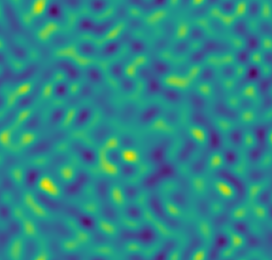
\includegraphics[interpolate=true,width=2.520000in,height=2.380000in]{burgers_solution_0.0-img0.png}}%
\end{pgfscope}%
\begin{pgfscope}%
\pgfsetbuttcap%
\pgfsetroundjoin%
\definecolor{currentfill}{rgb}{0.000000,0.000000,0.000000}%
\pgfsetfillcolor{currentfill}%
\pgfsetlinewidth{0.803000pt}%
\definecolor{currentstroke}{rgb}{0.000000,0.000000,0.000000}%
\pgfsetstrokecolor{currentstroke}%
\pgfsetdash{}{0pt}%
\pgfsys@defobject{currentmarker}{\pgfqpoint{0.000000in}{-0.048611in}}{\pgfqpoint{0.000000in}{0.000000in}}{%
\pgfpathmoveto{\pgfqpoint{0.000000in}{0.000000in}}%
\pgfpathlineto{\pgfqpoint{0.000000in}{-0.048611in}}%
\pgfusepath{stroke,fill}%
}%
\begin{pgfscope}%
\pgfsys@transformshift{0.567820in}{0.517039in}%
\pgfsys@useobject{currentmarker}{}%
\end{pgfscope}%
\end{pgfscope}%
\begin{pgfscope}%
\definecolor{textcolor}{rgb}{0.000000,0.000000,0.000000}%
\pgfsetstrokecolor{textcolor}%
\pgfsetfillcolor{textcolor}%
\pgftext[x=0.567820in,y=0.419816in,,top]{\color{textcolor}{\rmfamily\fontsize{12.000000}{14.400000}\selectfont\catcode`\^=\active\def^{\ifmmode\sp\else\^{}\fi}\catcode`\%=\active\def%{\%}0.0}}%
\end{pgfscope}%
\begin{pgfscope}%
\pgfsetbuttcap%
\pgfsetroundjoin%
\definecolor{currentfill}{rgb}{0.000000,0.000000,0.000000}%
\pgfsetfillcolor{currentfill}%
\pgfsetlinewidth{0.803000pt}%
\definecolor{currentstroke}{rgb}{0.000000,0.000000,0.000000}%
\pgfsetstrokecolor{currentstroke}%
\pgfsetdash{}{0pt}%
\pgfsys@defobject{currentmarker}{\pgfqpoint{0.000000in}{-0.048611in}}{\pgfqpoint{0.000000in}{0.000000in}}{%
\pgfpathmoveto{\pgfqpoint{0.000000in}{0.000000in}}%
\pgfpathlineto{\pgfqpoint{0.000000in}{-0.048611in}}%
\pgfusepath{stroke,fill}%
}%
\begin{pgfscope}%
\pgfsys@transformshift{1.196524in}{0.517039in}%
\pgfsys@useobject{currentmarker}{}%
\end{pgfscope}%
\end{pgfscope}%
\begin{pgfscope}%
\definecolor{textcolor}{rgb}{0.000000,0.000000,0.000000}%
\pgfsetstrokecolor{textcolor}%
\pgfsetfillcolor{textcolor}%
\pgftext[x=1.196524in,y=0.419816in,,top]{\color{textcolor}{\rmfamily\fontsize{12.000000}{14.400000}\selectfont\catcode`\^=\active\def^{\ifmmode\sp\else\^{}\fi}\catcode`\%=\active\def%{\%}0.5}}%
\end{pgfscope}%
\begin{pgfscope}%
\pgfsetbuttcap%
\pgfsetroundjoin%
\definecolor{currentfill}{rgb}{0.000000,0.000000,0.000000}%
\pgfsetfillcolor{currentfill}%
\pgfsetlinewidth{0.803000pt}%
\definecolor{currentstroke}{rgb}{0.000000,0.000000,0.000000}%
\pgfsetstrokecolor{currentstroke}%
\pgfsetdash{}{0pt}%
\pgfsys@defobject{currentmarker}{\pgfqpoint{0.000000in}{-0.048611in}}{\pgfqpoint{0.000000in}{0.000000in}}{%
\pgfpathmoveto{\pgfqpoint{0.000000in}{0.000000in}}%
\pgfpathlineto{\pgfqpoint{0.000000in}{-0.048611in}}%
\pgfusepath{stroke,fill}%
}%
\begin{pgfscope}%
\pgfsys@transformshift{1.825229in}{0.517039in}%
\pgfsys@useobject{currentmarker}{}%
\end{pgfscope}%
\end{pgfscope}%
\begin{pgfscope}%
\definecolor{textcolor}{rgb}{0.000000,0.000000,0.000000}%
\pgfsetstrokecolor{textcolor}%
\pgfsetfillcolor{textcolor}%
\pgftext[x=1.825229in,y=0.419816in,,top]{\color{textcolor}{\rmfamily\fontsize{12.000000}{14.400000}\selectfont\catcode`\^=\active\def^{\ifmmode\sp\else\^{}\fi}\catcode`\%=\active\def%{\%}1.0}}%
\end{pgfscope}%
\begin{pgfscope}%
\pgfsetbuttcap%
\pgfsetroundjoin%
\definecolor{currentfill}{rgb}{0.000000,0.000000,0.000000}%
\pgfsetfillcolor{currentfill}%
\pgfsetlinewidth{0.803000pt}%
\definecolor{currentstroke}{rgb}{0.000000,0.000000,0.000000}%
\pgfsetstrokecolor{currentstroke}%
\pgfsetdash{}{0pt}%
\pgfsys@defobject{currentmarker}{\pgfqpoint{0.000000in}{-0.048611in}}{\pgfqpoint{0.000000in}{0.000000in}}{%
\pgfpathmoveto{\pgfqpoint{0.000000in}{0.000000in}}%
\pgfpathlineto{\pgfqpoint{0.000000in}{-0.048611in}}%
\pgfusepath{stroke,fill}%
}%
\begin{pgfscope}%
\pgfsys@transformshift{2.453933in}{0.517039in}%
\pgfsys@useobject{currentmarker}{}%
\end{pgfscope}%
\end{pgfscope}%
\begin{pgfscope}%
\definecolor{textcolor}{rgb}{0.000000,0.000000,0.000000}%
\pgfsetstrokecolor{textcolor}%
\pgfsetfillcolor{textcolor}%
\pgftext[x=2.453933in,y=0.419816in,,top]{\color{textcolor}{\rmfamily\fontsize{12.000000}{14.400000}\selectfont\catcode`\^=\active\def^{\ifmmode\sp\else\^{}\fi}\catcode`\%=\active\def%{\%}1.5}}%
\end{pgfscope}%
\begin{pgfscope}%
\pgfsetbuttcap%
\pgfsetroundjoin%
\definecolor{currentfill}{rgb}{0.000000,0.000000,0.000000}%
\pgfsetfillcolor{currentfill}%
\pgfsetlinewidth{0.803000pt}%
\definecolor{currentstroke}{rgb}{0.000000,0.000000,0.000000}%
\pgfsetstrokecolor{currentstroke}%
\pgfsetdash{}{0pt}%
\pgfsys@defobject{currentmarker}{\pgfqpoint{0.000000in}{-0.048611in}}{\pgfqpoint{0.000000in}{0.000000in}}{%
\pgfpathmoveto{\pgfqpoint{0.000000in}{0.000000in}}%
\pgfpathlineto{\pgfqpoint{0.000000in}{-0.048611in}}%
\pgfusepath{stroke,fill}%
}%
\begin{pgfscope}%
\pgfsys@transformshift{3.082637in}{0.517039in}%
\pgfsys@useobject{currentmarker}{}%
\end{pgfscope}%
\end{pgfscope}%
\begin{pgfscope}%
\definecolor{textcolor}{rgb}{0.000000,0.000000,0.000000}%
\pgfsetstrokecolor{textcolor}%
\pgfsetfillcolor{textcolor}%
\pgftext[x=3.082637in,y=0.419816in,,top]{\color{textcolor}{\rmfamily\fontsize{12.000000}{14.400000}\selectfont\catcode`\^=\active\def^{\ifmmode\sp\else\^{}\fi}\catcode`\%=\active\def%{\%}2.0}}%
\end{pgfscope}%
\begin{pgfscope}%
\definecolor{textcolor}{rgb}{0.000000,0.000000,0.000000}%
\pgfsetstrokecolor{textcolor}%
\pgfsetfillcolor{textcolor}%
\pgftext[x=1.825229in,y=0.202965in,,top]{\color{textcolor}{\rmfamily\fontsize{12.000000}{14.400000}\selectfont\catcode`\^=\active\def^{\ifmmode\sp\else\^{}\fi}\catcode`\%=\active\def%{\%}Space}}%
\end{pgfscope}%
\begin{pgfscope}%
\pgfsetbuttcap%
\pgfsetroundjoin%
\definecolor{currentfill}{rgb}{0.000000,0.000000,0.000000}%
\pgfsetfillcolor{currentfill}%
\pgfsetlinewidth{0.803000pt}%
\definecolor{currentstroke}{rgb}{0.000000,0.000000,0.000000}%
\pgfsetstrokecolor{currentstroke}%
\pgfsetdash{}{0pt}%
\pgfsys@defobject{currentmarker}{\pgfqpoint{-0.048611in}{0.000000in}}{\pgfqpoint{-0.000000in}{0.000000in}}{%
\pgfpathmoveto{\pgfqpoint{-0.000000in}{0.000000in}}%
\pgfpathlineto{\pgfqpoint{-0.048611in}{0.000000in}}%
\pgfusepath{stroke,fill}%
}%
\begin{pgfscope}%
\pgfsys@transformshift{0.567820in}{0.517039in}%
\pgfsys@useobject{currentmarker}{}%
\end{pgfscope}%
\end{pgfscope}%
\begin{pgfscope}%
\definecolor{textcolor}{rgb}{0.000000,0.000000,0.000000}%
\pgfsetstrokecolor{textcolor}%
\pgfsetfillcolor{textcolor}%
\pgftext[x=0.364559in, y=0.453725in, left, base]{\color{textcolor}{\rmfamily\fontsize{12.000000}{14.400000}\selectfont\catcode`\^=\active\def^{\ifmmode\sp\else\^{}\fi}\catcode`\%=\active\def%{\%}0}}%
\end{pgfscope}%
\begin{pgfscope}%
\pgfsetbuttcap%
\pgfsetroundjoin%
\definecolor{currentfill}{rgb}{0.000000,0.000000,0.000000}%
\pgfsetfillcolor{currentfill}%
\pgfsetlinewidth{0.803000pt}%
\definecolor{currentstroke}{rgb}{0.000000,0.000000,0.000000}%
\pgfsetstrokecolor{currentstroke}%
\pgfsetdash{}{0pt}%
\pgfsys@defobject{currentmarker}{\pgfqpoint{-0.048611in}{0.000000in}}{\pgfqpoint{-0.000000in}{0.000000in}}{%
\pgfpathmoveto{\pgfqpoint{-0.000000in}{0.000000in}}%
\pgfpathlineto{\pgfqpoint{-0.048611in}{0.000000in}}%
\pgfusepath{stroke,fill}%
}%
\begin{pgfscope}%
\pgfsys@transformshift{0.567820in}{0.992634in}%
\pgfsys@useobject{currentmarker}{}%
\end{pgfscope}%
\end{pgfscope}%
\begin{pgfscope}%
\definecolor{textcolor}{rgb}{0.000000,0.000000,0.000000}%
\pgfsetstrokecolor{textcolor}%
\pgfsetfillcolor{textcolor}%
\pgftext[x=0.364559in, y=0.929320in, left, base]{\color{textcolor}{\rmfamily\fontsize{12.000000}{14.400000}\selectfont\catcode`\^=\active\def^{\ifmmode\sp\else\^{}\fi}\catcode`\%=\active\def%{\%}2}}%
\end{pgfscope}%
\begin{pgfscope}%
\pgfsetbuttcap%
\pgfsetroundjoin%
\definecolor{currentfill}{rgb}{0.000000,0.000000,0.000000}%
\pgfsetfillcolor{currentfill}%
\pgfsetlinewidth{0.803000pt}%
\definecolor{currentstroke}{rgb}{0.000000,0.000000,0.000000}%
\pgfsetstrokecolor{currentstroke}%
\pgfsetdash{}{0pt}%
\pgfsys@defobject{currentmarker}{\pgfqpoint{-0.048611in}{0.000000in}}{\pgfqpoint{-0.000000in}{0.000000in}}{%
\pgfpathmoveto{\pgfqpoint{-0.000000in}{0.000000in}}%
\pgfpathlineto{\pgfqpoint{-0.048611in}{0.000000in}}%
\pgfusepath{stroke,fill}%
}%
\begin{pgfscope}%
\pgfsys@transformshift{0.567820in}{1.468230in}%
\pgfsys@useobject{currentmarker}{}%
\end{pgfscope}%
\end{pgfscope}%
\begin{pgfscope}%
\definecolor{textcolor}{rgb}{0.000000,0.000000,0.000000}%
\pgfsetstrokecolor{textcolor}%
\pgfsetfillcolor{textcolor}%
\pgftext[x=0.364559in, y=1.404916in, left, base]{\color{textcolor}{\rmfamily\fontsize{12.000000}{14.400000}\selectfont\catcode`\^=\active\def^{\ifmmode\sp\else\^{}\fi}\catcode`\%=\active\def%{\%}4}}%
\end{pgfscope}%
\begin{pgfscope}%
\pgfsetbuttcap%
\pgfsetroundjoin%
\definecolor{currentfill}{rgb}{0.000000,0.000000,0.000000}%
\pgfsetfillcolor{currentfill}%
\pgfsetlinewidth{0.803000pt}%
\definecolor{currentstroke}{rgb}{0.000000,0.000000,0.000000}%
\pgfsetstrokecolor{currentstroke}%
\pgfsetdash{}{0pt}%
\pgfsys@defobject{currentmarker}{\pgfqpoint{-0.048611in}{0.000000in}}{\pgfqpoint{-0.000000in}{0.000000in}}{%
\pgfpathmoveto{\pgfqpoint{-0.000000in}{0.000000in}}%
\pgfpathlineto{\pgfqpoint{-0.048611in}{0.000000in}}%
\pgfusepath{stroke,fill}%
}%
\begin{pgfscope}%
\pgfsys@transformshift{0.567820in}{1.943825in}%
\pgfsys@useobject{currentmarker}{}%
\end{pgfscope}%
\end{pgfscope}%
\begin{pgfscope}%
\definecolor{textcolor}{rgb}{0.000000,0.000000,0.000000}%
\pgfsetstrokecolor{textcolor}%
\pgfsetfillcolor{textcolor}%
\pgftext[x=0.364559in, y=1.880511in, left, base]{\color{textcolor}{\rmfamily\fontsize{12.000000}{14.400000}\selectfont\catcode`\^=\active\def^{\ifmmode\sp\else\^{}\fi}\catcode`\%=\active\def%{\%}6}}%
\end{pgfscope}%
\begin{pgfscope}%
\pgfsetbuttcap%
\pgfsetroundjoin%
\definecolor{currentfill}{rgb}{0.000000,0.000000,0.000000}%
\pgfsetfillcolor{currentfill}%
\pgfsetlinewidth{0.803000pt}%
\definecolor{currentstroke}{rgb}{0.000000,0.000000,0.000000}%
\pgfsetstrokecolor{currentstroke}%
\pgfsetdash{}{0pt}%
\pgfsys@defobject{currentmarker}{\pgfqpoint{-0.048611in}{0.000000in}}{\pgfqpoint{-0.000000in}{0.000000in}}{%
\pgfpathmoveto{\pgfqpoint{-0.000000in}{0.000000in}}%
\pgfpathlineto{\pgfqpoint{-0.048611in}{0.000000in}}%
\pgfusepath{stroke,fill}%
}%
\begin{pgfscope}%
\pgfsys@transformshift{0.567820in}{2.419421in}%
\pgfsys@useobject{currentmarker}{}%
\end{pgfscope}%
\end{pgfscope}%
\begin{pgfscope}%
\definecolor{textcolor}{rgb}{0.000000,0.000000,0.000000}%
\pgfsetstrokecolor{textcolor}%
\pgfsetfillcolor{textcolor}%
\pgftext[x=0.364559in, y=2.356107in, left, base]{\color{textcolor}{\rmfamily\fontsize{12.000000}{14.400000}\selectfont\catcode`\^=\active\def^{\ifmmode\sp\else\^{}\fi}\catcode`\%=\active\def%{\%}8}}%
\end{pgfscope}%
\begin{pgfscope}%
\pgfsetbuttcap%
\pgfsetroundjoin%
\definecolor{currentfill}{rgb}{0.000000,0.000000,0.000000}%
\pgfsetfillcolor{currentfill}%
\pgfsetlinewidth{0.803000pt}%
\definecolor{currentstroke}{rgb}{0.000000,0.000000,0.000000}%
\pgfsetstrokecolor{currentstroke}%
\pgfsetdash{}{0pt}%
\pgfsys@defobject{currentmarker}{\pgfqpoint{-0.048611in}{0.000000in}}{\pgfqpoint{-0.000000in}{0.000000in}}{%
\pgfpathmoveto{\pgfqpoint{-0.000000in}{0.000000in}}%
\pgfpathlineto{\pgfqpoint{-0.048611in}{0.000000in}}%
\pgfusepath{stroke,fill}%
}%
\begin{pgfscope}%
\pgfsys@transformshift{0.567820in}{2.895016in}%
\pgfsys@useobject{currentmarker}{}%
\end{pgfscope}%
\end{pgfscope}%
\begin{pgfscope}%
\definecolor{textcolor}{rgb}{0.000000,0.000000,0.000000}%
\pgfsetstrokecolor{textcolor}%
\pgfsetfillcolor{textcolor}%
\pgftext[x=0.258521in, y=2.831702in, left, base]{\color{textcolor}{\rmfamily\fontsize{12.000000}{14.400000}\selectfont\catcode`\^=\active\def^{\ifmmode\sp\else\^{}\fi}\catcode`\%=\active\def%{\%}10}}%
\end{pgfscope}%
\begin{pgfscope}%
\definecolor{textcolor}{rgb}{0.000000,0.000000,0.000000}%
\pgfsetstrokecolor{textcolor}%
\pgfsetfillcolor{textcolor}%
\pgftext[x=0.202965in,y=1.706027in,,bottom,rotate=90.000000]{\color{textcolor}{\rmfamily\fontsize{12.000000}{14.400000}\selectfont\catcode`\^=\active\def^{\ifmmode\sp\else\^{}\fi}\catcode`\%=\active\def%{\%}Time}}%
\end{pgfscope}%
\begin{pgfscope}%
\pgfsetrectcap%
\pgfsetmiterjoin%
\pgfsetlinewidth{0.803000pt}%
\definecolor{currentstroke}{rgb}{0.000000,0.000000,0.000000}%
\pgfsetstrokecolor{currentstroke}%
\pgfsetdash{}{0pt}%
\pgfpathmoveto{\pgfqpoint{0.567820in}{0.517039in}}%
\pgfpathlineto{\pgfqpoint{0.567820in}{2.895016in}}%
\pgfusepath{stroke}%
\end{pgfscope}%
\begin{pgfscope}%
\pgfsetrectcap%
\pgfsetmiterjoin%
\pgfsetlinewidth{0.803000pt}%
\definecolor{currentstroke}{rgb}{0.000000,0.000000,0.000000}%
\pgfsetstrokecolor{currentstroke}%
\pgfsetdash{}{0pt}%
\pgfpathmoveto{\pgfqpoint{3.082637in}{0.517039in}}%
\pgfpathlineto{\pgfqpoint{3.082637in}{2.895016in}}%
\pgfusepath{stroke}%
\end{pgfscope}%
\begin{pgfscope}%
\pgfsetrectcap%
\pgfsetmiterjoin%
\pgfsetlinewidth{0.803000pt}%
\definecolor{currentstroke}{rgb}{0.000000,0.000000,0.000000}%
\pgfsetstrokecolor{currentstroke}%
\pgfsetdash{}{0pt}%
\pgfpathmoveto{\pgfqpoint{0.567820in}{0.517039in}}%
\pgfpathlineto{\pgfqpoint{3.082637in}{0.517039in}}%
\pgfusepath{stroke}%
\end{pgfscope}%
\begin{pgfscope}%
\pgfsetrectcap%
\pgfsetmiterjoin%
\pgfsetlinewidth{0.803000pt}%
\definecolor{currentstroke}{rgb}{0.000000,0.000000,0.000000}%
\pgfsetstrokecolor{currentstroke}%
\pgfsetdash{}{0pt}%
\pgfpathmoveto{\pgfqpoint{0.567820in}{2.895016in}}%
\pgfpathlineto{\pgfqpoint{3.082637in}{2.895016in}}%
\pgfusepath{stroke}%
\end{pgfscope}%
\begin{pgfscope}%
\pgfsetbuttcap%
\pgfsetmiterjoin%
\pgfsetlinewidth{0.000000pt}%
\definecolor{currentstroke}{rgb}{0.000000,0.000000,0.000000}%
\pgfsetstrokecolor{currentstroke}%
\pgfsetstrokeopacity{0.000000}%
\pgfsetdash{}{0pt}%
\pgfpathmoveto{\pgfqpoint{3.340906in}{0.517039in}}%
\pgfpathlineto{\pgfqpoint{3.459805in}{0.517039in}}%
\pgfpathlineto{\pgfqpoint{3.459805in}{2.895016in}}%
\pgfpathlineto{\pgfqpoint{3.340906in}{2.895016in}}%
\pgfpathlineto{\pgfqpoint{3.340906in}{0.517039in}}%
\pgfpathclose%
\pgfusepath{}%
\end{pgfscope}%
\begin{pgfscope}%
\pgfsys@transformshift{3.340000in}{0.520000in}%
\pgftext[left,bottom]{
\includegraphics[interpolate=true,width=0.120000in,height=2.380000in]{burgers_solution_0.0-img1.png}}%
\end{pgfscope}%
\begin{pgfscope}%
\pgfsetbuttcap%
\pgfsetroundjoin%
\definecolor{currentfill}{rgb}{0.000000,0.000000,0.000000}%
\pgfsetfillcolor{currentfill}%
\pgfsetlinewidth{0.803000pt}%
\definecolor{currentstroke}{rgb}{0.000000,0.000000,0.000000}%
\pgfsetstrokecolor{currentstroke}%
\pgfsetdash{}{0pt}%
\pgfsys@defobject{currentmarker}{\pgfqpoint{0.000000in}{0.000000in}}{\pgfqpoint{0.048611in}{0.000000in}}{%
\pgfpathmoveto{\pgfqpoint{0.000000in}{0.000000in}}%
\pgfpathlineto{\pgfqpoint{0.048611in}{0.000000in}}%
\pgfusepath{stroke,fill}%
}%
\begin{pgfscope}%
\pgfsys@transformshift{3.459805in}{0.555741in}%
\pgfsys@useobject{currentmarker}{}%
\end{pgfscope}%
\end{pgfscope}%
\begin{pgfscope}%
\definecolor{textcolor}{rgb}{0.000000,0.000000,0.000000}%
\pgfsetstrokecolor{textcolor}%
\pgfsetfillcolor{textcolor}%
\pgftext[x=3.557027in, y=0.492427in, left, base]{\color{textcolor}{\rmfamily\fontsize{12.000000}{14.400000}\selectfont\catcode`\^=\active\def^{\ifmmode\sp\else\^{}\fi}\catcode`\%=\active\def%{\%}\ensuremath{-}0.6}}%
\end{pgfscope}%
\begin{pgfscope}%
\pgfsetbuttcap%
\pgfsetroundjoin%
\definecolor{currentfill}{rgb}{0.000000,0.000000,0.000000}%
\pgfsetfillcolor{currentfill}%
\pgfsetlinewidth{0.803000pt}%
\definecolor{currentstroke}{rgb}{0.000000,0.000000,0.000000}%
\pgfsetstrokecolor{currentstroke}%
\pgfsetdash{}{0pt}%
\pgfsys@defobject{currentmarker}{\pgfqpoint{0.000000in}{0.000000in}}{\pgfqpoint{0.048611in}{0.000000in}}{%
\pgfpathmoveto{\pgfqpoint{0.000000in}{0.000000in}}%
\pgfpathlineto{\pgfqpoint{0.048611in}{0.000000in}}%
\pgfusepath{stroke,fill}%
}%
\begin{pgfscope}%
\pgfsys@transformshift{3.459805in}{0.932008in}%
\pgfsys@useobject{currentmarker}{}%
\end{pgfscope}%
\end{pgfscope}%
\begin{pgfscope}%
\definecolor{textcolor}{rgb}{0.000000,0.000000,0.000000}%
\pgfsetstrokecolor{textcolor}%
\pgfsetfillcolor{textcolor}%
\pgftext[x=3.557027in, y=0.868694in, left, base]{\color{textcolor}{\rmfamily\fontsize{12.000000}{14.400000}\selectfont\catcode`\^=\active\def^{\ifmmode\sp\else\^{}\fi}\catcode`\%=\active\def%{\%}\ensuremath{-}0.4}}%
\end{pgfscope}%
\begin{pgfscope}%
\pgfsetbuttcap%
\pgfsetroundjoin%
\definecolor{currentfill}{rgb}{0.000000,0.000000,0.000000}%
\pgfsetfillcolor{currentfill}%
\pgfsetlinewidth{0.803000pt}%
\definecolor{currentstroke}{rgb}{0.000000,0.000000,0.000000}%
\pgfsetstrokecolor{currentstroke}%
\pgfsetdash{}{0pt}%
\pgfsys@defobject{currentmarker}{\pgfqpoint{0.000000in}{0.000000in}}{\pgfqpoint{0.048611in}{0.000000in}}{%
\pgfpathmoveto{\pgfqpoint{0.000000in}{0.000000in}}%
\pgfpathlineto{\pgfqpoint{0.048611in}{0.000000in}}%
\pgfusepath{stroke,fill}%
}%
\begin{pgfscope}%
\pgfsys@transformshift{3.459805in}{1.308274in}%
\pgfsys@useobject{currentmarker}{}%
\end{pgfscope}%
\end{pgfscope}%
\begin{pgfscope}%
\definecolor{textcolor}{rgb}{0.000000,0.000000,0.000000}%
\pgfsetstrokecolor{textcolor}%
\pgfsetfillcolor{textcolor}%
\pgftext[x=3.557027in, y=1.244961in, left, base]{\color{textcolor}{\rmfamily\fontsize{12.000000}{14.400000}\selectfont\catcode`\^=\active\def^{\ifmmode\sp\else\^{}\fi}\catcode`\%=\active\def%{\%}\ensuremath{-}0.2}}%
\end{pgfscope}%
\begin{pgfscope}%
\pgfsetbuttcap%
\pgfsetroundjoin%
\definecolor{currentfill}{rgb}{0.000000,0.000000,0.000000}%
\pgfsetfillcolor{currentfill}%
\pgfsetlinewidth{0.803000pt}%
\definecolor{currentstroke}{rgb}{0.000000,0.000000,0.000000}%
\pgfsetstrokecolor{currentstroke}%
\pgfsetdash{}{0pt}%
\pgfsys@defobject{currentmarker}{\pgfqpoint{0.000000in}{0.000000in}}{\pgfqpoint{0.048611in}{0.000000in}}{%
\pgfpathmoveto{\pgfqpoint{0.000000in}{0.000000in}}%
\pgfpathlineto{\pgfqpoint{0.048611in}{0.000000in}}%
\pgfusepath{stroke,fill}%
}%
\begin{pgfscope}%
\pgfsys@transformshift{3.459805in}{1.684541in}%
\pgfsys@useobject{currentmarker}{}%
\end{pgfscope}%
\end{pgfscope}%
\begin{pgfscope}%
\definecolor{textcolor}{rgb}{0.000000,0.000000,0.000000}%
\pgfsetstrokecolor{textcolor}%
\pgfsetfillcolor{textcolor}%
\pgftext[x=3.557027in, y=1.621228in, left, base]{\color{textcolor}{\rmfamily\fontsize{12.000000}{14.400000}\selectfont\catcode`\^=\active\def^{\ifmmode\sp\else\^{}\fi}\catcode`\%=\active\def%{\%}0.0}}%
\end{pgfscope}%
\begin{pgfscope}%
\pgfsetbuttcap%
\pgfsetroundjoin%
\definecolor{currentfill}{rgb}{0.000000,0.000000,0.000000}%
\pgfsetfillcolor{currentfill}%
\pgfsetlinewidth{0.803000pt}%
\definecolor{currentstroke}{rgb}{0.000000,0.000000,0.000000}%
\pgfsetstrokecolor{currentstroke}%
\pgfsetdash{}{0pt}%
\pgfsys@defobject{currentmarker}{\pgfqpoint{0.000000in}{0.000000in}}{\pgfqpoint{0.048611in}{0.000000in}}{%
\pgfpathmoveto{\pgfqpoint{0.000000in}{0.000000in}}%
\pgfpathlineto{\pgfqpoint{0.048611in}{0.000000in}}%
\pgfusepath{stroke,fill}%
}%
\begin{pgfscope}%
\pgfsys@transformshift{3.459805in}{2.060808in}%
\pgfsys@useobject{currentmarker}{}%
\end{pgfscope}%
\end{pgfscope}%
\begin{pgfscope}%
\definecolor{textcolor}{rgb}{0.000000,0.000000,0.000000}%
\pgfsetstrokecolor{textcolor}%
\pgfsetfillcolor{textcolor}%
\pgftext[x=3.557027in, y=1.997494in, left, base]{\color{textcolor}{\rmfamily\fontsize{12.000000}{14.400000}\selectfont\catcode`\^=\active\def^{\ifmmode\sp\else\^{}\fi}\catcode`\%=\active\def%{\%}0.2}}%
\end{pgfscope}%
\begin{pgfscope}%
\pgfsetbuttcap%
\pgfsetroundjoin%
\definecolor{currentfill}{rgb}{0.000000,0.000000,0.000000}%
\pgfsetfillcolor{currentfill}%
\pgfsetlinewidth{0.803000pt}%
\definecolor{currentstroke}{rgb}{0.000000,0.000000,0.000000}%
\pgfsetstrokecolor{currentstroke}%
\pgfsetdash{}{0pt}%
\pgfsys@defobject{currentmarker}{\pgfqpoint{0.000000in}{0.000000in}}{\pgfqpoint{0.048611in}{0.000000in}}{%
\pgfpathmoveto{\pgfqpoint{0.000000in}{0.000000in}}%
\pgfpathlineto{\pgfqpoint{0.048611in}{0.000000in}}%
\pgfusepath{stroke,fill}%
}%
\begin{pgfscope}%
\pgfsys@transformshift{3.459805in}{2.437075in}%
\pgfsys@useobject{currentmarker}{}%
\end{pgfscope}%
\end{pgfscope}%
\begin{pgfscope}%
\definecolor{textcolor}{rgb}{0.000000,0.000000,0.000000}%
\pgfsetstrokecolor{textcolor}%
\pgfsetfillcolor{textcolor}%
\pgftext[x=3.557027in, y=2.373761in, left, base]{\color{textcolor}{\rmfamily\fontsize{12.000000}{14.400000}\selectfont\catcode`\^=\active\def^{\ifmmode\sp\else\^{}\fi}\catcode`\%=\active\def%{\%}0.4}}%
\end{pgfscope}%
\begin{pgfscope}%
\pgfsetbuttcap%
\pgfsetroundjoin%
\definecolor{currentfill}{rgb}{0.000000,0.000000,0.000000}%
\pgfsetfillcolor{currentfill}%
\pgfsetlinewidth{0.803000pt}%
\definecolor{currentstroke}{rgb}{0.000000,0.000000,0.000000}%
\pgfsetstrokecolor{currentstroke}%
\pgfsetdash{}{0pt}%
\pgfsys@defobject{currentmarker}{\pgfqpoint{0.000000in}{0.000000in}}{\pgfqpoint{0.048611in}{0.000000in}}{%
\pgfpathmoveto{\pgfqpoint{0.000000in}{0.000000in}}%
\pgfpathlineto{\pgfqpoint{0.048611in}{0.000000in}}%
\pgfusepath{stroke,fill}%
}%
\begin{pgfscope}%
\pgfsys@transformshift{3.459805in}{2.813342in}%
\pgfsys@useobject{currentmarker}{}%
\end{pgfscope}%
\end{pgfscope}%
\begin{pgfscope}%
\definecolor{textcolor}{rgb}{0.000000,0.000000,0.000000}%
\pgfsetstrokecolor{textcolor}%
\pgfsetfillcolor{textcolor}%
\pgftext[x=3.557027in, y=2.750028in, left, base]{\color{textcolor}{\rmfamily\fontsize{12.000000}{14.400000}\selectfont\catcode`\^=\active\def^{\ifmmode\sp\else\^{}\fi}\catcode`\%=\active\def%{\%}0.6}}%
\end{pgfscope}%
\begin{pgfscope}%
\pgfsetrectcap%
\pgfsetmiterjoin%
\pgfsetlinewidth{0.803000pt}%
\definecolor{currentstroke}{rgb}{0.000000,0.000000,0.000000}%
\pgfsetstrokecolor{currentstroke}%
\pgfsetdash{}{0pt}%
\pgfpathmoveto{\pgfqpoint{3.340906in}{0.517039in}}%
\pgfpathlineto{\pgfqpoint{3.400355in}{0.517039in}}%
\pgfpathlineto{\pgfqpoint{3.459805in}{0.517039in}}%
\pgfpathlineto{\pgfqpoint{3.459805in}{2.895016in}}%
\pgfpathlineto{\pgfqpoint{3.400355in}{2.895016in}}%
\pgfpathlineto{\pgfqpoint{3.340906in}{2.895016in}}%
\pgfpathlineto{\pgfqpoint{3.340906in}{0.517039in}}%
\pgfpathclose%
\pgfusepath{stroke}%
\end{pgfscope}%
\end{pgfpicture}%
\makeatother%
\endgroup%

    \end{adjustbox}
    \caption{Solution function for \(\nu=0\).}\label{fig:burgers_solution_0.0}
  \end{subfigure}
  \begin{subfigure}{0.49\linewidth}
    \begin{adjustbox}{width=\linewidth}
      \begingroup%
\makeatletter%
\begin{pgfpicture}%
\pgfpathrectangle{\pgfpointorigin}{\pgfqpoint{4.000000in}{3.000000in}}%
\pgfusepath{use as bounding box, clip}%
\begin{pgfscope}%
\pgfsetbuttcap%
\pgfsetmiterjoin%
\pgfsetlinewidth{0.000000pt}%
\definecolor{currentstroke}{rgb}{0.000000,0.000000,0.000000}%
\pgfsetstrokecolor{currentstroke}%
\pgfsetstrokeopacity{0.000000}%
\pgfsetdash{}{0pt}%
\pgfpathmoveto{\pgfqpoint{0.000000in}{0.000000in}}%
\pgfpathlineto{\pgfqpoint{4.000000in}{0.000000in}}%
\pgfpathlineto{\pgfqpoint{4.000000in}{3.000000in}}%
\pgfpathlineto{\pgfqpoint{0.000000in}{3.000000in}}%
\pgfpathlineto{\pgfqpoint{0.000000in}{0.000000in}}%
\pgfpathclose%
\pgfusepath{}%
\end{pgfscope}%
\begin{pgfscope}%
\pgfsetbuttcap%
\pgfsetmiterjoin%
\pgfsetlinewidth{0.000000pt}%
\definecolor{currentstroke}{rgb}{0.000000,0.000000,0.000000}%
\pgfsetstrokecolor{currentstroke}%
\pgfsetstrokeopacity{0.000000}%
\pgfsetdash{}{0pt}%
\pgfpathmoveto{\pgfqpoint{0.567820in}{0.517039in}}%
\pgfpathlineto{\pgfqpoint{3.082637in}{0.517039in}}%
\pgfpathlineto{\pgfqpoint{3.082637in}{2.895016in}}%
\pgfpathlineto{\pgfqpoint{0.567820in}{2.895016in}}%
\pgfpathlineto{\pgfqpoint{0.567820in}{0.517039in}}%
\pgfpathclose%
\pgfusepath{}%
\end{pgfscope}%
\begin{pgfscope}%
\pgfpathrectangle{\pgfqpoint{0.567820in}{0.517039in}}{\pgfqpoint{2.514817in}{2.377978in}}%
\pgfusepath{clip}%
\pgfsys@transformshift{0.567820in}{0.517039in}%
\pgftext[left,bottom]{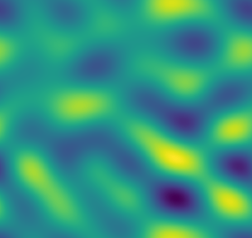
\includegraphics[interpolate=true,width=2.520000in,height=2.380000in]{burgers_forcing_0.0-img0.png}}%
\end{pgfscope}%
\begin{pgfscope}%
\pgfsetbuttcap%
\pgfsetroundjoin%
\definecolor{currentfill}{rgb}{0.000000,0.000000,0.000000}%
\pgfsetfillcolor{currentfill}%
\pgfsetlinewidth{0.803000pt}%
\definecolor{currentstroke}{rgb}{0.000000,0.000000,0.000000}%
\pgfsetstrokecolor{currentstroke}%
\pgfsetdash{}{0pt}%
\pgfsys@defobject{currentmarker}{\pgfqpoint{0.000000in}{-0.048611in}}{\pgfqpoint{0.000000in}{0.000000in}}{%
\pgfpathmoveto{\pgfqpoint{0.000000in}{0.000000in}}%
\pgfpathlineto{\pgfqpoint{0.000000in}{-0.048611in}}%
\pgfusepath{stroke,fill}%
}%
\begin{pgfscope}%
\pgfsys@transformshift{0.567820in}{0.517039in}%
\pgfsys@useobject{currentmarker}{}%
\end{pgfscope}%
\end{pgfscope}%
\begin{pgfscope}%
\definecolor{textcolor}{rgb}{0.000000,0.000000,0.000000}%
\pgfsetstrokecolor{textcolor}%
\pgfsetfillcolor{textcolor}%
\pgftext[x=0.567820in,y=0.419816in,,top]{\color{textcolor}{\rmfamily\fontsize{12.000000}{14.400000}\selectfont\catcode`\^=\active\def^{\ifmmode\sp\else\^{}\fi}\catcode`\%=\active\def%{\%}0.0}}%
\end{pgfscope}%
\begin{pgfscope}%
\pgfsetbuttcap%
\pgfsetroundjoin%
\definecolor{currentfill}{rgb}{0.000000,0.000000,0.000000}%
\pgfsetfillcolor{currentfill}%
\pgfsetlinewidth{0.803000pt}%
\definecolor{currentstroke}{rgb}{0.000000,0.000000,0.000000}%
\pgfsetstrokecolor{currentstroke}%
\pgfsetdash{}{0pt}%
\pgfsys@defobject{currentmarker}{\pgfqpoint{0.000000in}{-0.048611in}}{\pgfqpoint{0.000000in}{0.000000in}}{%
\pgfpathmoveto{\pgfqpoint{0.000000in}{0.000000in}}%
\pgfpathlineto{\pgfqpoint{0.000000in}{-0.048611in}}%
\pgfusepath{stroke,fill}%
}%
\begin{pgfscope}%
\pgfsys@transformshift{1.196524in}{0.517039in}%
\pgfsys@useobject{currentmarker}{}%
\end{pgfscope}%
\end{pgfscope}%
\begin{pgfscope}%
\definecolor{textcolor}{rgb}{0.000000,0.000000,0.000000}%
\pgfsetstrokecolor{textcolor}%
\pgfsetfillcolor{textcolor}%
\pgftext[x=1.196524in,y=0.419816in,,top]{\color{textcolor}{\rmfamily\fontsize{12.000000}{14.400000}\selectfont\catcode`\^=\active\def^{\ifmmode\sp\else\^{}\fi}\catcode`\%=\active\def%{\%}0.5}}%
\end{pgfscope}%
\begin{pgfscope}%
\pgfsetbuttcap%
\pgfsetroundjoin%
\definecolor{currentfill}{rgb}{0.000000,0.000000,0.000000}%
\pgfsetfillcolor{currentfill}%
\pgfsetlinewidth{0.803000pt}%
\definecolor{currentstroke}{rgb}{0.000000,0.000000,0.000000}%
\pgfsetstrokecolor{currentstroke}%
\pgfsetdash{}{0pt}%
\pgfsys@defobject{currentmarker}{\pgfqpoint{0.000000in}{-0.048611in}}{\pgfqpoint{0.000000in}{0.000000in}}{%
\pgfpathmoveto{\pgfqpoint{0.000000in}{0.000000in}}%
\pgfpathlineto{\pgfqpoint{0.000000in}{-0.048611in}}%
\pgfusepath{stroke,fill}%
}%
\begin{pgfscope}%
\pgfsys@transformshift{1.825229in}{0.517039in}%
\pgfsys@useobject{currentmarker}{}%
\end{pgfscope}%
\end{pgfscope}%
\begin{pgfscope}%
\definecolor{textcolor}{rgb}{0.000000,0.000000,0.000000}%
\pgfsetstrokecolor{textcolor}%
\pgfsetfillcolor{textcolor}%
\pgftext[x=1.825229in,y=0.419816in,,top]{\color{textcolor}{\rmfamily\fontsize{12.000000}{14.400000}\selectfont\catcode`\^=\active\def^{\ifmmode\sp\else\^{}\fi}\catcode`\%=\active\def%{\%}1.0}}%
\end{pgfscope}%
\begin{pgfscope}%
\pgfsetbuttcap%
\pgfsetroundjoin%
\definecolor{currentfill}{rgb}{0.000000,0.000000,0.000000}%
\pgfsetfillcolor{currentfill}%
\pgfsetlinewidth{0.803000pt}%
\definecolor{currentstroke}{rgb}{0.000000,0.000000,0.000000}%
\pgfsetstrokecolor{currentstroke}%
\pgfsetdash{}{0pt}%
\pgfsys@defobject{currentmarker}{\pgfqpoint{0.000000in}{-0.048611in}}{\pgfqpoint{0.000000in}{0.000000in}}{%
\pgfpathmoveto{\pgfqpoint{0.000000in}{0.000000in}}%
\pgfpathlineto{\pgfqpoint{0.000000in}{-0.048611in}}%
\pgfusepath{stroke,fill}%
}%
\begin{pgfscope}%
\pgfsys@transformshift{2.453933in}{0.517039in}%
\pgfsys@useobject{currentmarker}{}%
\end{pgfscope}%
\end{pgfscope}%
\begin{pgfscope}%
\definecolor{textcolor}{rgb}{0.000000,0.000000,0.000000}%
\pgfsetstrokecolor{textcolor}%
\pgfsetfillcolor{textcolor}%
\pgftext[x=2.453933in,y=0.419816in,,top]{\color{textcolor}{\rmfamily\fontsize{12.000000}{14.400000}\selectfont\catcode`\^=\active\def^{\ifmmode\sp\else\^{}\fi}\catcode`\%=\active\def%{\%}1.5}}%
\end{pgfscope}%
\begin{pgfscope}%
\pgfsetbuttcap%
\pgfsetroundjoin%
\definecolor{currentfill}{rgb}{0.000000,0.000000,0.000000}%
\pgfsetfillcolor{currentfill}%
\pgfsetlinewidth{0.803000pt}%
\definecolor{currentstroke}{rgb}{0.000000,0.000000,0.000000}%
\pgfsetstrokecolor{currentstroke}%
\pgfsetdash{}{0pt}%
\pgfsys@defobject{currentmarker}{\pgfqpoint{0.000000in}{-0.048611in}}{\pgfqpoint{0.000000in}{0.000000in}}{%
\pgfpathmoveto{\pgfqpoint{0.000000in}{0.000000in}}%
\pgfpathlineto{\pgfqpoint{0.000000in}{-0.048611in}}%
\pgfusepath{stroke,fill}%
}%
\begin{pgfscope}%
\pgfsys@transformshift{3.082637in}{0.517039in}%
\pgfsys@useobject{currentmarker}{}%
\end{pgfscope}%
\end{pgfscope}%
\begin{pgfscope}%
\definecolor{textcolor}{rgb}{0.000000,0.000000,0.000000}%
\pgfsetstrokecolor{textcolor}%
\pgfsetfillcolor{textcolor}%
\pgftext[x=3.082637in,y=0.419816in,,top]{\color{textcolor}{\rmfamily\fontsize{12.000000}{14.400000}\selectfont\catcode`\^=\active\def^{\ifmmode\sp\else\^{}\fi}\catcode`\%=\active\def%{\%}2.0}}%
\end{pgfscope}%
\begin{pgfscope}%
\definecolor{textcolor}{rgb}{0.000000,0.000000,0.000000}%
\pgfsetstrokecolor{textcolor}%
\pgfsetfillcolor{textcolor}%
\pgftext[x=1.825229in,y=0.202965in,,top]{\color{textcolor}{\rmfamily\fontsize{12.000000}{14.400000}\selectfont\catcode`\^=\active\def^{\ifmmode\sp\else\^{}\fi}\catcode`\%=\active\def%{\%}Space}}%
\end{pgfscope}%
\begin{pgfscope}%
\pgfsetbuttcap%
\pgfsetroundjoin%
\definecolor{currentfill}{rgb}{0.000000,0.000000,0.000000}%
\pgfsetfillcolor{currentfill}%
\pgfsetlinewidth{0.803000pt}%
\definecolor{currentstroke}{rgb}{0.000000,0.000000,0.000000}%
\pgfsetstrokecolor{currentstroke}%
\pgfsetdash{}{0pt}%
\pgfsys@defobject{currentmarker}{\pgfqpoint{-0.048611in}{0.000000in}}{\pgfqpoint{-0.000000in}{0.000000in}}{%
\pgfpathmoveto{\pgfqpoint{-0.000000in}{0.000000in}}%
\pgfpathlineto{\pgfqpoint{-0.048611in}{0.000000in}}%
\pgfusepath{stroke,fill}%
}%
\begin{pgfscope}%
\pgfsys@transformshift{0.567820in}{0.517039in}%
\pgfsys@useobject{currentmarker}{}%
\end{pgfscope}%
\end{pgfscope}%
\begin{pgfscope}%
\definecolor{textcolor}{rgb}{0.000000,0.000000,0.000000}%
\pgfsetstrokecolor{textcolor}%
\pgfsetfillcolor{textcolor}%
\pgftext[x=0.364559in, y=0.453725in, left, base]{\color{textcolor}{\rmfamily\fontsize{12.000000}{14.400000}\selectfont\catcode`\^=\active\def^{\ifmmode\sp\else\^{}\fi}\catcode`\%=\active\def%{\%}0}}%
\end{pgfscope}%
\begin{pgfscope}%
\pgfsetbuttcap%
\pgfsetroundjoin%
\definecolor{currentfill}{rgb}{0.000000,0.000000,0.000000}%
\pgfsetfillcolor{currentfill}%
\pgfsetlinewidth{0.803000pt}%
\definecolor{currentstroke}{rgb}{0.000000,0.000000,0.000000}%
\pgfsetstrokecolor{currentstroke}%
\pgfsetdash{}{0pt}%
\pgfsys@defobject{currentmarker}{\pgfqpoint{-0.048611in}{0.000000in}}{\pgfqpoint{-0.000000in}{0.000000in}}{%
\pgfpathmoveto{\pgfqpoint{-0.000000in}{0.000000in}}%
\pgfpathlineto{\pgfqpoint{-0.048611in}{0.000000in}}%
\pgfusepath{stroke,fill}%
}%
\begin{pgfscope}%
\pgfsys@transformshift{0.567820in}{0.992634in}%
\pgfsys@useobject{currentmarker}{}%
\end{pgfscope}%
\end{pgfscope}%
\begin{pgfscope}%
\definecolor{textcolor}{rgb}{0.000000,0.000000,0.000000}%
\pgfsetstrokecolor{textcolor}%
\pgfsetfillcolor{textcolor}%
\pgftext[x=0.364559in, y=0.929320in, left, base]{\color{textcolor}{\rmfamily\fontsize{12.000000}{14.400000}\selectfont\catcode`\^=\active\def^{\ifmmode\sp\else\^{}\fi}\catcode`\%=\active\def%{\%}2}}%
\end{pgfscope}%
\begin{pgfscope}%
\pgfsetbuttcap%
\pgfsetroundjoin%
\definecolor{currentfill}{rgb}{0.000000,0.000000,0.000000}%
\pgfsetfillcolor{currentfill}%
\pgfsetlinewidth{0.803000pt}%
\definecolor{currentstroke}{rgb}{0.000000,0.000000,0.000000}%
\pgfsetstrokecolor{currentstroke}%
\pgfsetdash{}{0pt}%
\pgfsys@defobject{currentmarker}{\pgfqpoint{-0.048611in}{0.000000in}}{\pgfqpoint{-0.000000in}{0.000000in}}{%
\pgfpathmoveto{\pgfqpoint{-0.000000in}{0.000000in}}%
\pgfpathlineto{\pgfqpoint{-0.048611in}{0.000000in}}%
\pgfusepath{stroke,fill}%
}%
\begin{pgfscope}%
\pgfsys@transformshift{0.567820in}{1.468230in}%
\pgfsys@useobject{currentmarker}{}%
\end{pgfscope}%
\end{pgfscope}%
\begin{pgfscope}%
\definecolor{textcolor}{rgb}{0.000000,0.000000,0.000000}%
\pgfsetstrokecolor{textcolor}%
\pgfsetfillcolor{textcolor}%
\pgftext[x=0.364559in, y=1.404916in, left, base]{\color{textcolor}{\rmfamily\fontsize{12.000000}{14.400000}\selectfont\catcode`\^=\active\def^{\ifmmode\sp\else\^{}\fi}\catcode`\%=\active\def%{\%}4}}%
\end{pgfscope}%
\begin{pgfscope}%
\pgfsetbuttcap%
\pgfsetroundjoin%
\definecolor{currentfill}{rgb}{0.000000,0.000000,0.000000}%
\pgfsetfillcolor{currentfill}%
\pgfsetlinewidth{0.803000pt}%
\definecolor{currentstroke}{rgb}{0.000000,0.000000,0.000000}%
\pgfsetstrokecolor{currentstroke}%
\pgfsetdash{}{0pt}%
\pgfsys@defobject{currentmarker}{\pgfqpoint{-0.048611in}{0.000000in}}{\pgfqpoint{-0.000000in}{0.000000in}}{%
\pgfpathmoveto{\pgfqpoint{-0.000000in}{0.000000in}}%
\pgfpathlineto{\pgfqpoint{-0.048611in}{0.000000in}}%
\pgfusepath{stroke,fill}%
}%
\begin{pgfscope}%
\pgfsys@transformshift{0.567820in}{1.943825in}%
\pgfsys@useobject{currentmarker}{}%
\end{pgfscope}%
\end{pgfscope}%
\begin{pgfscope}%
\definecolor{textcolor}{rgb}{0.000000,0.000000,0.000000}%
\pgfsetstrokecolor{textcolor}%
\pgfsetfillcolor{textcolor}%
\pgftext[x=0.364559in, y=1.880511in, left, base]{\color{textcolor}{\rmfamily\fontsize{12.000000}{14.400000}\selectfont\catcode`\^=\active\def^{\ifmmode\sp\else\^{}\fi}\catcode`\%=\active\def%{\%}6}}%
\end{pgfscope}%
\begin{pgfscope}%
\pgfsetbuttcap%
\pgfsetroundjoin%
\definecolor{currentfill}{rgb}{0.000000,0.000000,0.000000}%
\pgfsetfillcolor{currentfill}%
\pgfsetlinewidth{0.803000pt}%
\definecolor{currentstroke}{rgb}{0.000000,0.000000,0.000000}%
\pgfsetstrokecolor{currentstroke}%
\pgfsetdash{}{0pt}%
\pgfsys@defobject{currentmarker}{\pgfqpoint{-0.048611in}{0.000000in}}{\pgfqpoint{-0.000000in}{0.000000in}}{%
\pgfpathmoveto{\pgfqpoint{-0.000000in}{0.000000in}}%
\pgfpathlineto{\pgfqpoint{-0.048611in}{0.000000in}}%
\pgfusepath{stroke,fill}%
}%
\begin{pgfscope}%
\pgfsys@transformshift{0.567820in}{2.419421in}%
\pgfsys@useobject{currentmarker}{}%
\end{pgfscope}%
\end{pgfscope}%
\begin{pgfscope}%
\definecolor{textcolor}{rgb}{0.000000,0.000000,0.000000}%
\pgfsetstrokecolor{textcolor}%
\pgfsetfillcolor{textcolor}%
\pgftext[x=0.364559in, y=2.356107in, left, base]{\color{textcolor}{\rmfamily\fontsize{12.000000}{14.400000}\selectfont\catcode`\^=\active\def^{\ifmmode\sp\else\^{}\fi}\catcode`\%=\active\def%{\%}8}}%
\end{pgfscope}%
\begin{pgfscope}%
\pgfsetbuttcap%
\pgfsetroundjoin%
\definecolor{currentfill}{rgb}{0.000000,0.000000,0.000000}%
\pgfsetfillcolor{currentfill}%
\pgfsetlinewidth{0.803000pt}%
\definecolor{currentstroke}{rgb}{0.000000,0.000000,0.000000}%
\pgfsetstrokecolor{currentstroke}%
\pgfsetdash{}{0pt}%
\pgfsys@defobject{currentmarker}{\pgfqpoint{-0.048611in}{0.000000in}}{\pgfqpoint{-0.000000in}{0.000000in}}{%
\pgfpathmoveto{\pgfqpoint{-0.000000in}{0.000000in}}%
\pgfpathlineto{\pgfqpoint{-0.048611in}{0.000000in}}%
\pgfusepath{stroke,fill}%
}%
\begin{pgfscope}%
\pgfsys@transformshift{0.567820in}{2.895016in}%
\pgfsys@useobject{currentmarker}{}%
\end{pgfscope}%
\end{pgfscope}%
\begin{pgfscope}%
\definecolor{textcolor}{rgb}{0.000000,0.000000,0.000000}%
\pgfsetstrokecolor{textcolor}%
\pgfsetfillcolor{textcolor}%
\pgftext[x=0.258521in, y=2.831702in, left, base]{\color{textcolor}{\rmfamily\fontsize{12.000000}{14.400000}\selectfont\catcode`\^=\active\def^{\ifmmode\sp\else\^{}\fi}\catcode`\%=\active\def%{\%}10}}%
\end{pgfscope}%
\begin{pgfscope}%
\definecolor{textcolor}{rgb}{0.000000,0.000000,0.000000}%
\pgfsetstrokecolor{textcolor}%
\pgfsetfillcolor{textcolor}%
\pgftext[x=0.202965in,y=1.706027in,,bottom,rotate=90.000000]{\color{textcolor}{\rmfamily\fontsize{12.000000}{14.400000}\selectfont\catcode`\^=\active\def^{\ifmmode\sp\else\^{}\fi}\catcode`\%=\active\def%{\%}Time}}%
\end{pgfscope}%
\begin{pgfscope}%
\pgfsetrectcap%
\pgfsetmiterjoin%
\pgfsetlinewidth{0.803000pt}%
\definecolor{currentstroke}{rgb}{0.000000,0.000000,0.000000}%
\pgfsetstrokecolor{currentstroke}%
\pgfsetdash{}{0pt}%
\pgfpathmoveto{\pgfqpoint{0.567820in}{0.517039in}}%
\pgfpathlineto{\pgfqpoint{0.567820in}{2.895016in}}%
\pgfusepath{stroke}%
\end{pgfscope}%
\begin{pgfscope}%
\pgfsetrectcap%
\pgfsetmiterjoin%
\pgfsetlinewidth{0.803000pt}%
\definecolor{currentstroke}{rgb}{0.000000,0.000000,0.000000}%
\pgfsetstrokecolor{currentstroke}%
\pgfsetdash{}{0pt}%
\pgfpathmoveto{\pgfqpoint{3.082637in}{0.517039in}}%
\pgfpathlineto{\pgfqpoint{3.082637in}{2.895016in}}%
\pgfusepath{stroke}%
\end{pgfscope}%
\begin{pgfscope}%
\pgfsetrectcap%
\pgfsetmiterjoin%
\pgfsetlinewidth{0.803000pt}%
\definecolor{currentstroke}{rgb}{0.000000,0.000000,0.000000}%
\pgfsetstrokecolor{currentstroke}%
\pgfsetdash{}{0pt}%
\pgfpathmoveto{\pgfqpoint{0.567820in}{0.517039in}}%
\pgfpathlineto{\pgfqpoint{3.082637in}{0.517039in}}%
\pgfusepath{stroke}%
\end{pgfscope}%
\begin{pgfscope}%
\pgfsetrectcap%
\pgfsetmiterjoin%
\pgfsetlinewidth{0.803000pt}%
\definecolor{currentstroke}{rgb}{0.000000,0.000000,0.000000}%
\pgfsetstrokecolor{currentstroke}%
\pgfsetdash{}{0pt}%
\pgfpathmoveto{\pgfqpoint{0.567820in}{2.895016in}}%
\pgfpathlineto{\pgfqpoint{3.082637in}{2.895016in}}%
\pgfusepath{stroke}%
\end{pgfscope}%
\begin{pgfscope}%
\pgfsetbuttcap%
\pgfsetmiterjoin%
\pgfsetlinewidth{0.000000pt}%
\definecolor{currentstroke}{rgb}{0.000000,0.000000,0.000000}%
\pgfsetstrokecolor{currentstroke}%
\pgfsetstrokeopacity{0.000000}%
\pgfsetdash{}{0pt}%
\pgfpathmoveto{\pgfqpoint{3.340906in}{0.517039in}}%
\pgfpathlineto{\pgfqpoint{3.459805in}{0.517039in}}%
\pgfpathlineto{\pgfqpoint{3.459805in}{2.895016in}}%
\pgfpathlineto{\pgfqpoint{3.340906in}{2.895016in}}%
\pgfpathlineto{\pgfqpoint{3.340906in}{0.517039in}}%
\pgfpathclose%
\pgfusepath{}%
\end{pgfscope}%
\begin{pgfscope}%
\pgfsys@transformshift{3.340000in}{0.520000in}%
\pgftext[left,bottom]{
\includegraphics[interpolate=true,width=0.120000in,height=2.380000in]{burgers_forcing_0.0-img1.png}}%
\end{pgfscope}%
\begin{pgfscope}%
\pgfsetbuttcap%
\pgfsetroundjoin%
\definecolor{currentfill}{rgb}{0.000000,0.000000,0.000000}%
\pgfsetfillcolor{currentfill}%
\pgfsetlinewidth{0.803000pt}%
\definecolor{currentstroke}{rgb}{0.000000,0.000000,0.000000}%
\pgfsetstrokecolor{currentstroke}%
\pgfsetdash{}{0pt}%
\pgfsys@defobject{currentmarker}{\pgfqpoint{0.000000in}{0.000000in}}{\pgfqpoint{0.048611in}{0.000000in}}{%
\pgfpathmoveto{\pgfqpoint{0.000000in}{0.000000in}}%
\pgfpathlineto{\pgfqpoint{0.048611in}{0.000000in}}%
\pgfusepath{stroke,fill}%
}%
\begin{pgfscope}%
\pgfsys@transformshift{3.459805in}{0.595621in}%
\pgfsys@useobject{currentmarker}{}%
\end{pgfscope}%
\end{pgfscope}%
\begin{pgfscope}%
\definecolor{textcolor}{rgb}{0.000000,0.000000,0.000000}%
\pgfsetstrokecolor{textcolor}%
\pgfsetfillcolor{textcolor}%
\pgftext[x=3.557027in, y=0.532307in, left, base]{\color{textcolor}{\rmfamily\fontsize{12.000000}{14.400000}\selectfont\catcode`\^=\active\def^{\ifmmode\sp\else\^{}\fi}\catcode`\%=\active\def%{\%}\ensuremath{-}1.0}}%
\end{pgfscope}%
\begin{pgfscope}%
\pgfsetbuttcap%
\pgfsetroundjoin%
\definecolor{currentfill}{rgb}{0.000000,0.000000,0.000000}%
\pgfsetfillcolor{currentfill}%
\pgfsetlinewidth{0.803000pt}%
\definecolor{currentstroke}{rgb}{0.000000,0.000000,0.000000}%
\pgfsetstrokecolor{currentstroke}%
\pgfsetdash{}{0pt}%
\pgfsys@defobject{currentmarker}{\pgfqpoint{0.000000in}{0.000000in}}{\pgfqpoint{0.048611in}{0.000000in}}{%
\pgfpathmoveto{\pgfqpoint{0.000000in}{0.000000in}}%
\pgfpathlineto{\pgfqpoint{0.048611in}{0.000000in}}%
\pgfusepath{stroke,fill}%
}%
\begin{pgfscope}%
\pgfsys@transformshift{3.459805in}{1.192198in}%
\pgfsys@useobject{currentmarker}{}%
\end{pgfscope}%
\end{pgfscope}%
\begin{pgfscope}%
\definecolor{textcolor}{rgb}{0.000000,0.000000,0.000000}%
\pgfsetstrokecolor{textcolor}%
\pgfsetfillcolor{textcolor}%
\pgftext[x=3.557027in, y=1.128884in, left, base]{\color{textcolor}{\rmfamily\fontsize{12.000000}{14.400000}\selectfont\catcode`\^=\active\def^{\ifmmode\sp\else\^{}\fi}\catcode`\%=\active\def%{\%}\ensuremath{-}0.5}}%
\end{pgfscope}%
\begin{pgfscope}%
\pgfsetbuttcap%
\pgfsetroundjoin%
\definecolor{currentfill}{rgb}{0.000000,0.000000,0.000000}%
\pgfsetfillcolor{currentfill}%
\pgfsetlinewidth{0.803000pt}%
\definecolor{currentstroke}{rgb}{0.000000,0.000000,0.000000}%
\pgfsetstrokecolor{currentstroke}%
\pgfsetdash{}{0pt}%
\pgfsys@defobject{currentmarker}{\pgfqpoint{0.000000in}{0.000000in}}{\pgfqpoint{0.048611in}{0.000000in}}{%
\pgfpathmoveto{\pgfqpoint{0.000000in}{0.000000in}}%
\pgfpathlineto{\pgfqpoint{0.048611in}{0.000000in}}%
\pgfusepath{stroke,fill}%
}%
\begin{pgfscope}%
\pgfsys@transformshift{3.459805in}{1.788774in}%
\pgfsys@useobject{currentmarker}{}%
\end{pgfscope}%
\end{pgfscope}%
\begin{pgfscope}%
\definecolor{textcolor}{rgb}{0.000000,0.000000,0.000000}%
\pgfsetstrokecolor{textcolor}%
\pgfsetfillcolor{textcolor}%
\pgftext[x=3.557027in, y=1.725460in, left, base]{\color{textcolor}{\rmfamily\fontsize{12.000000}{14.400000}\selectfont\catcode`\^=\active\def^{\ifmmode\sp\else\^{}\fi}\catcode`\%=\active\def%{\%}0.0}}%
\end{pgfscope}%
\begin{pgfscope}%
\pgfsetbuttcap%
\pgfsetroundjoin%
\definecolor{currentfill}{rgb}{0.000000,0.000000,0.000000}%
\pgfsetfillcolor{currentfill}%
\pgfsetlinewidth{0.803000pt}%
\definecolor{currentstroke}{rgb}{0.000000,0.000000,0.000000}%
\pgfsetstrokecolor{currentstroke}%
\pgfsetdash{}{0pt}%
\pgfsys@defobject{currentmarker}{\pgfqpoint{0.000000in}{0.000000in}}{\pgfqpoint{0.048611in}{0.000000in}}{%
\pgfpathmoveto{\pgfqpoint{0.000000in}{0.000000in}}%
\pgfpathlineto{\pgfqpoint{0.048611in}{0.000000in}}%
\pgfusepath{stroke,fill}%
}%
\begin{pgfscope}%
\pgfsys@transformshift{3.459805in}{2.385351in}%
\pgfsys@useobject{currentmarker}{}%
\end{pgfscope}%
\end{pgfscope}%
\begin{pgfscope}%
\definecolor{textcolor}{rgb}{0.000000,0.000000,0.000000}%
\pgfsetstrokecolor{textcolor}%
\pgfsetfillcolor{textcolor}%
\pgftext[x=3.557027in, y=2.322037in, left, base]{\color{textcolor}{\rmfamily\fontsize{12.000000}{14.400000}\selectfont\catcode`\^=\active\def^{\ifmmode\sp\else\^{}\fi}\catcode`\%=\active\def%{\%}0.5}}%
\end{pgfscope}%
\begin{pgfscope}%
\pgfsetrectcap%
\pgfsetmiterjoin%
\pgfsetlinewidth{0.803000pt}%
\definecolor{currentstroke}{rgb}{0.000000,0.000000,0.000000}%
\pgfsetstrokecolor{currentstroke}%
\pgfsetdash{}{0pt}%
\pgfpathmoveto{\pgfqpoint{3.340906in}{0.517039in}}%
\pgfpathlineto{\pgfqpoint{3.400355in}{0.517039in}}%
\pgfpathlineto{\pgfqpoint{3.459805in}{0.517039in}}%
\pgfpathlineto{\pgfqpoint{3.459805in}{2.895016in}}%
\pgfpathlineto{\pgfqpoint{3.400355in}{2.895016in}}%
\pgfpathlineto{\pgfqpoint{3.340906in}{2.895016in}}%
\pgfpathlineto{\pgfqpoint{3.340906in}{0.517039in}}%
\pgfpathclose%
\pgfusepath{stroke}%
\end{pgfscope}%
\end{pgfpicture}%
\makeatother%
\endgroup%

    \end{adjustbox}
    \caption{Forcing function for \(\nu=0\).}\label{fig:burgers_forcing_0.0}
  \end{subfigure}
  % \\[-0.7\baselineskip]
  \begin{subfigure}{0.49\linewidth}
    \begin{adjustbox}{width=\linewidth}
      \begingroup%
\makeatletter%
\begin{pgfpicture}%
\pgfpathrectangle{\pgfpointorigin}{\pgfqpoint{4.000000in}{3.000000in}}%
\pgfusepath{use as bounding box, clip}%
\begin{pgfscope}%
\pgfsetbuttcap%
\pgfsetmiterjoin%
\pgfsetlinewidth{0.000000pt}%
\definecolor{currentstroke}{rgb}{0.000000,0.000000,0.000000}%
\pgfsetstrokecolor{currentstroke}%
\pgfsetstrokeopacity{0.000000}%
\pgfsetdash{}{0pt}%
\pgfpathmoveto{\pgfqpoint{0.000000in}{0.000000in}}%
\pgfpathlineto{\pgfqpoint{4.000000in}{0.000000in}}%
\pgfpathlineto{\pgfqpoint{4.000000in}{3.000000in}}%
\pgfpathlineto{\pgfqpoint{0.000000in}{3.000000in}}%
\pgfpathlineto{\pgfqpoint{0.000000in}{0.000000in}}%
\pgfpathclose%
\pgfusepath{}%
\end{pgfscope}%
\begin{pgfscope}%
\pgfsetbuttcap%
\pgfsetmiterjoin%
\pgfsetlinewidth{0.000000pt}%
\definecolor{currentstroke}{rgb}{0.000000,0.000000,0.000000}%
\pgfsetstrokecolor{currentstroke}%
\pgfsetstrokeopacity{0.000000}%
\pgfsetdash{}{0pt}%
\pgfpathmoveto{\pgfqpoint{0.567820in}{0.517039in}}%
\pgfpathlineto{\pgfqpoint{3.082637in}{0.517039in}}%
\pgfpathlineto{\pgfqpoint{3.082637in}{2.895016in}}%
\pgfpathlineto{\pgfqpoint{0.567820in}{2.895016in}}%
\pgfpathlineto{\pgfqpoint{0.567820in}{0.517039in}}%
\pgfpathclose%
\pgfusepath{}%
\end{pgfscope}%
\begin{pgfscope}%
\pgfpathrectangle{\pgfqpoint{0.567820in}{0.517039in}}{\pgfqpoint{2.514817in}{2.377978in}}%
\pgfusepath{clip}%
\pgfsys@transformshift{0.567820in}{0.517039in}%
\pgftext[left,bottom]{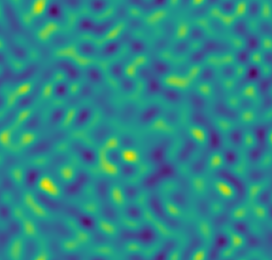
\includegraphics[interpolate=true,width=2.520000in,height=2.380000in]{burgers_solution_0.01-img0.png}}%
\end{pgfscope}%
\begin{pgfscope}%
\pgfsetbuttcap%
\pgfsetroundjoin%
\definecolor{currentfill}{rgb}{0.000000,0.000000,0.000000}%
\pgfsetfillcolor{currentfill}%
\pgfsetlinewidth{0.803000pt}%
\definecolor{currentstroke}{rgb}{0.000000,0.000000,0.000000}%
\pgfsetstrokecolor{currentstroke}%
\pgfsetdash{}{0pt}%
\pgfsys@defobject{currentmarker}{\pgfqpoint{0.000000in}{-0.048611in}}{\pgfqpoint{0.000000in}{0.000000in}}{%
\pgfpathmoveto{\pgfqpoint{0.000000in}{0.000000in}}%
\pgfpathlineto{\pgfqpoint{0.000000in}{-0.048611in}}%
\pgfusepath{stroke,fill}%
}%
\begin{pgfscope}%
\pgfsys@transformshift{0.567820in}{0.517039in}%
\pgfsys@useobject{currentmarker}{}%
\end{pgfscope}%
\end{pgfscope}%
\begin{pgfscope}%
\definecolor{textcolor}{rgb}{0.000000,0.000000,0.000000}%
\pgfsetstrokecolor{textcolor}%
\pgfsetfillcolor{textcolor}%
\pgftext[x=0.567820in,y=0.419816in,,top]{\color{textcolor}\rmfamily\fontsize{12.000000}{14.400000}\selectfont 0.0}%
\end{pgfscope}%
\begin{pgfscope}%
\pgfsetbuttcap%
\pgfsetroundjoin%
\definecolor{currentfill}{rgb}{0.000000,0.000000,0.000000}%
\pgfsetfillcolor{currentfill}%
\pgfsetlinewidth{0.803000pt}%
\definecolor{currentstroke}{rgb}{0.000000,0.000000,0.000000}%
\pgfsetstrokecolor{currentstroke}%
\pgfsetdash{}{0pt}%
\pgfsys@defobject{currentmarker}{\pgfqpoint{0.000000in}{-0.048611in}}{\pgfqpoint{0.000000in}{0.000000in}}{%
\pgfpathmoveto{\pgfqpoint{0.000000in}{0.000000in}}%
\pgfpathlineto{\pgfqpoint{0.000000in}{-0.048611in}}%
\pgfusepath{stroke,fill}%
}%
\begin{pgfscope}%
\pgfsys@transformshift{1.196524in}{0.517039in}%
\pgfsys@useobject{currentmarker}{}%
\end{pgfscope}%
\end{pgfscope}%
\begin{pgfscope}%
\definecolor{textcolor}{rgb}{0.000000,0.000000,0.000000}%
\pgfsetstrokecolor{textcolor}%
\pgfsetfillcolor{textcolor}%
\pgftext[x=1.196524in,y=0.419816in,,top]{\color{textcolor}\rmfamily\fontsize{12.000000}{14.400000}\selectfont 0.5}%
\end{pgfscope}%
\begin{pgfscope}%
\pgfsetbuttcap%
\pgfsetroundjoin%
\definecolor{currentfill}{rgb}{0.000000,0.000000,0.000000}%
\pgfsetfillcolor{currentfill}%
\pgfsetlinewidth{0.803000pt}%
\definecolor{currentstroke}{rgb}{0.000000,0.000000,0.000000}%
\pgfsetstrokecolor{currentstroke}%
\pgfsetdash{}{0pt}%
\pgfsys@defobject{currentmarker}{\pgfqpoint{0.000000in}{-0.048611in}}{\pgfqpoint{0.000000in}{0.000000in}}{%
\pgfpathmoveto{\pgfqpoint{0.000000in}{0.000000in}}%
\pgfpathlineto{\pgfqpoint{0.000000in}{-0.048611in}}%
\pgfusepath{stroke,fill}%
}%
\begin{pgfscope}%
\pgfsys@transformshift{1.825229in}{0.517039in}%
\pgfsys@useobject{currentmarker}{}%
\end{pgfscope}%
\end{pgfscope}%
\begin{pgfscope}%
\definecolor{textcolor}{rgb}{0.000000,0.000000,0.000000}%
\pgfsetstrokecolor{textcolor}%
\pgfsetfillcolor{textcolor}%
\pgftext[x=1.825229in,y=0.419816in,,top]{\color{textcolor}\rmfamily\fontsize{12.000000}{14.400000}\selectfont 1.0}%
\end{pgfscope}%
\begin{pgfscope}%
\pgfsetbuttcap%
\pgfsetroundjoin%
\definecolor{currentfill}{rgb}{0.000000,0.000000,0.000000}%
\pgfsetfillcolor{currentfill}%
\pgfsetlinewidth{0.803000pt}%
\definecolor{currentstroke}{rgb}{0.000000,0.000000,0.000000}%
\pgfsetstrokecolor{currentstroke}%
\pgfsetdash{}{0pt}%
\pgfsys@defobject{currentmarker}{\pgfqpoint{0.000000in}{-0.048611in}}{\pgfqpoint{0.000000in}{0.000000in}}{%
\pgfpathmoveto{\pgfqpoint{0.000000in}{0.000000in}}%
\pgfpathlineto{\pgfqpoint{0.000000in}{-0.048611in}}%
\pgfusepath{stroke,fill}%
}%
\begin{pgfscope}%
\pgfsys@transformshift{2.453933in}{0.517039in}%
\pgfsys@useobject{currentmarker}{}%
\end{pgfscope}%
\end{pgfscope}%
\begin{pgfscope}%
\definecolor{textcolor}{rgb}{0.000000,0.000000,0.000000}%
\pgfsetstrokecolor{textcolor}%
\pgfsetfillcolor{textcolor}%
\pgftext[x=2.453933in,y=0.419816in,,top]{\color{textcolor}\rmfamily\fontsize{12.000000}{14.400000}\selectfont 1.5}%
\end{pgfscope}%
\begin{pgfscope}%
\pgfsetbuttcap%
\pgfsetroundjoin%
\definecolor{currentfill}{rgb}{0.000000,0.000000,0.000000}%
\pgfsetfillcolor{currentfill}%
\pgfsetlinewidth{0.803000pt}%
\definecolor{currentstroke}{rgb}{0.000000,0.000000,0.000000}%
\pgfsetstrokecolor{currentstroke}%
\pgfsetdash{}{0pt}%
\pgfsys@defobject{currentmarker}{\pgfqpoint{0.000000in}{-0.048611in}}{\pgfqpoint{0.000000in}{0.000000in}}{%
\pgfpathmoveto{\pgfqpoint{0.000000in}{0.000000in}}%
\pgfpathlineto{\pgfqpoint{0.000000in}{-0.048611in}}%
\pgfusepath{stroke,fill}%
}%
\begin{pgfscope}%
\pgfsys@transformshift{3.082637in}{0.517039in}%
\pgfsys@useobject{currentmarker}{}%
\end{pgfscope}%
\end{pgfscope}%
\begin{pgfscope}%
\definecolor{textcolor}{rgb}{0.000000,0.000000,0.000000}%
\pgfsetstrokecolor{textcolor}%
\pgfsetfillcolor{textcolor}%
\pgftext[x=3.082637in,y=0.419816in,,top]{\color{textcolor}\rmfamily\fontsize{12.000000}{14.400000}\selectfont 2.0}%
\end{pgfscope}%
\begin{pgfscope}%
\definecolor{textcolor}{rgb}{0.000000,0.000000,0.000000}%
\pgfsetstrokecolor{textcolor}%
\pgfsetfillcolor{textcolor}%
\pgftext[x=1.825229in,y=0.202965in,,top]{\color{textcolor}\rmfamily\fontsize{12.000000}{14.400000}\selectfont Space}%
\end{pgfscope}%
\begin{pgfscope}%
\pgfsetbuttcap%
\pgfsetroundjoin%
\definecolor{currentfill}{rgb}{0.000000,0.000000,0.000000}%
\pgfsetfillcolor{currentfill}%
\pgfsetlinewidth{0.803000pt}%
\definecolor{currentstroke}{rgb}{0.000000,0.000000,0.000000}%
\pgfsetstrokecolor{currentstroke}%
\pgfsetdash{}{0pt}%
\pgfsys@defobject{currentmarker}{\pgfqpoint{-0.048611in}{0.000000in}}{\pgfqpoint{-0.000000in}{0.000000in}}{%
\pgfpathmoveto{\pgfqpoint{-0.000000in}{0.000000in}}%
\pgfpathlineto{\pgfqpoint{-0.048611in}{0.000000in}}%
\pgfusepath{stroke,fill}%
}%
\begin{pgfscope}%
\pgfsys@transformshift{0.567820in}{0.517039in}%
\pgfsys@useobject{currentmarker}{}%
\end{pgfscope}%
\end{pgfscope}%
\begin{pgfscope}%
\definecolor{textcolor}{rgb}{0.000000,0.000000,0.000000}%
\pgfsetstrokecolor{textcolor}%
\pgfsetfillcolor{textcolor}%
\pgftext[x=0.364559in, y=0.453725in, left, base]{\color{textcolor}\rmfamily\fontsize{12.000000}{14.400000}\selectfont 0}%
\end{pgfscope}%
\begin{pgfscope}%
\pgfsetbuttcap%
\pgfsetroundjoin%
\definecolor{currentfill}{rgb}{0.000000,0.000000,0.000000}%
\pgfsetfillcolor{currentfill}%
\pgfsetlinewidth{0.803000pt}%
\definecolor{currentstroke}{rgb}{0.000000,0.000000,0.000000}%
\pgfsetstrokecolor{currentstroke}%
\pgfsetdash{}{0pt}%
\pgfsys@defobject{currentmarker}{\pgfqpoint{-0.048611in}{0.000000in}}{\pgfqpoint{-0.000000in}{0.000000in}}{%
\pgfpathmoveto{\pgfqpoint{-0.000000in}{0.000000in}}%
\pgfpathlineto{\pgfqpoint{-0.048611in}{0.000000in}}%
\pgfusepath{stroke,fill}%
}%
\begin{pgfscope}%
\pgfsys@transformshift{0.567820in}{0.992634in}%
\pgfsys@useobject{currentmarker}{}%
\end{pgfscope}%
\end{pgfscope}%
\begin{pgfscope}%
\definecolor{textcolor}{rgb}{0.000000,0.000000,0.000000}%
\pgfsetstrokecolor{textcolor}%
\pgfsetfillcolor{textcolor}%
\pgftext[x=0.364559in, y=0.929320in, left, base]{\color{textcolor}\rmfamily\fontsize{12.000000}{14.400000}\selectfont 2}%
\end{pgfscope}%
\begin{pgfscope}%
\pgfsetbuttcap%
\pgfsetroundjoin%
\definecolor{currentfill}{rgb}{0.000000,0.000000,0.000000}%
\pgfsetfillcolor{currentfill}%
\pgfsetlinewidth{0.803000pt}%
\definecolor{currentstroke}{rgb}{0.000000,0.000000,0.000000}%
\pgfsetstrokecolor{currentstroke}%
\pgfsetdash{}{0pt}%
\pgfsys@defobject{currentmarker}{\pgfqpoint{-0.048611in}{0.000000in}}{\pgfqpoint{-0.000000in}{0.000000in}}{%
\pgfpathmoveto{\pgfqpoint{-0.000000in}{0.000000in}}%
\pgfpathlineto{\pgfqpoint{-0.048611in}{0.000000in}}%
\pgfusepath{stroke,fill}%
}%
\begin{pgfscope}%
\pgfsys@transformshift{0.567820in}{1.468230in}%
\pgfsys@useobject{currentmarker}{}%
\end{pgfscope}%
\end{pgfscope}%
\begin{pgfscope}%
\definecolor{textcolor}{rgb}{0.000000,0.000000,0.000000}%
\pgfsetstrokecolor{textcolor}%
\pgfsetfillcolor{textcolor}%
\pgftext[x=0.364559in, y=1.404916in, left, base]{\color{textcolor}\rmfamily\fontsize{12.000000}{14.400000}\selectfont 4}%
\end{pgfscope}%
\begin{pgfscope}%
\pgfsetbuttcap%
\pgfsetroundjoin%
\definecolor{currentfill}{rgb}{0.000000,0.000000,0.000000}%
\pgfsetfillcolor{currentfill}%
\pgfsetlinewidth{0.803000pt}%
\definecolor{currentstroke}{rgb}{0.000000,0.000000,0.000000}%
\pgfsetstrokecolor{currentstroke}%
\pgfsetdash{}{0pt}%
\pgfsys@defobject{currentmarker}{\pgfqpoint{-0.048611in}{0.000000in}}{\pgfqpoint{-0.000000in}{0.000000in}}{%
\pgfpathmoveto{\pgfqpoint{-0.000000in}{0.000000in}}%
\pgfpathlineto{\pgfqpoint{-0.048611in}{0.000000in}}%
\pgfusepath{stroke,fill}%
}%
\begin{pgfscope}%
\pgfsys@transformshift{0.567820in}{1.943825in}%
\pgfsys@useobject{currentmarker}{}%
\end{pgfscope}%
\end{pgfscope}%
\begin{pgfscope}%
\definecolor{textcolor}{rgb}{0.000000,0.000000,0.000000}%
\pgfsetstrokecolor{textcolor}%
\pgfsetfillcolor{textcolor}%
\pgftext[x=0.364559in, y=1.880511in, left, base]{\color{textcolor}\rmfamily\fontsize{12.000000}{14.400000}\selectfont 6}%
\end{pgfscope}%
\begin{pgfscope}%
\pgfsetbuttcap%
\pgfsetroundjoin%
\definecolor{currentfill}{rgb}{0.000000,0.000000,0.000000}%
\pgfsetfillcolor{currentfill}%
\pgfsetlinewidth{0.803000pt}%
\definecolor{currentstroke}{rgb}{0.000000,0.000000,0.000000}%
\pgfsetstrokecolor{currentstroke}%
\pgfsetdash{}{0pt}%
\pgfsys@defobject{currentmarker}{\pgfqpoint{-0.048611in}{0.000000in}}{\pgfqpoint{-0.000000in}{0.000000in}}{%
\pgfpathmoveto{\pgfqpoint{-0.000000in}{0.000000in}}%
\pgfpathlineto{\pgfqpoint{-0.048611in}{0.000000in}}%
\pgfusepath{stroke,fill}%
}%
\begin{pgfscope}%
\pgfsys@transformshift{0.567820in}{2.419421in}%
\pgfsys@useobject{currentmarker}{}%
\end{pgfscope}%
\end{pgfscope}%
\begin{pgfscope}%
\definecolor{textcolor}{rgb}{0.000000,0.000000,0.000000}%
\pgfsetstrokecolor{textcolor}%
\pgfsetfillcolor{textcolor}%
\pgftext[x=0.364559in, y=2.356107in, left, base]{\color{textcolor}\rmfamily\fontsize{12.000000}{14.400000}\selectfont 8}%
\end{pgfscope}%
\begin{pgfscope}%
\pgfsetbuttcap%
\pgfsetroundjoin%
\definecolor{currentfill}{rgb}{0.000000,0.000000,0.000000}%
\pgfsetfillcolor{currentfill}%
\pgfsetlinewidth{0.803000pt}%
\definecolor{currentstroke}{rgb}{0.000000,0.000000,0.000000}%
\pgfsetstrokecolor{currentstroke}%
\pgfsetdash{}{0pt}%
\pgfsys@defobject{currentmarker}{\pgfqpoint{-0.048611in}{0.000000in}}{\pgfqpoint{-0.000000in}{0.000000in}}{%
\pgfpathmoveto{\pgfqpoint{-0.000000in}{0.000000in}}%
\pgfpathlineto{\pgfqpoint{-0.048611in}{0.000000in}}%
\pgfusepath{stroke,fill}%
}%
\begin{pgfscope}%
\pgfsys@transformshift{0.567820in}{2.895016in}%
\pgfsys@useobject{currentmarker}{}%
\end{pgfscope}%
\end{pgfscope}%
\begin{pgfscope}%
\definecolor{textcolor}{rgb}{0.000000,0.000000,0.000000}%
\pgfsetstrokecolor{textcolor}%
\pgfsetfillcolor{textcolor}%
\pgftext[x=0.258521in, y=2.831702in, left, base]{\color{textcolor}\rmfamily\fontsize{12.000000}{14.400000}\selectfont 10}%
\end{pgfscope}%
\begin{pgfscope}%
\definecolor{textcolor}{rgb}{0.000000,0.000000,0.000000}%
\pgfsetstrokecolor{textcolor}%
\pgfsetfillcolor{textcolor}%
\pgftext[x=0.202965in,y=1.706027in,,bottom,rotate=90.000000]{\color{textcolor}\rmfamily\fontsize{12.000000}{14.400000}\selectfont Time}%
\end{pgfscope}%
\begin{pgfscope}%
\pgfsetrectcap%
\pgfsetmiterjoin%
\pgfsetlinewidth{0.803000pt}%
\definecolor{currentstroke}{rgb}{0.000000,0.000000,0.000000}%
\pgfsetstrokecolor{currentstroke}%
\pgfsetdash{}{0pt}%
\pgfpathmoveto{\pgfqpoint{0.567820in}{0.517039in}}%
\pgfpathlineto{\pgfqpoint{0.567820in}{2.895016in}}%
\pgfusepath{stroke}%
\end{pgfscope}%
\begin{pgfscope}%
\pgfsetrectcap%
\pgfsetmiterjoin%
\pgfsetlinewidth{0.803000pt}%
\definecolor{currentstroke}{rgb}{0.000000,0.000000,0.000000}%
\pgfsetstrokecolor{currentstroke}%
\pgfsetdash{}{0pt}%
\pgfpathmoveto{\pgfqpoint{3.082637in}{0.517039in}}%
\pgfpathlineto{\pgfqpoint{3.082637in}{2.895016in}}%
\pgfusepath{stroke}%
\end{pgfscope}%
\begin{pgfscope}%
\pgfsetrectcap%
\pgfsetmiterjoin%
\pgfsetlinewidth{0.803000pt}%
\definecolor{currentstroke}{rgb}{0.000000,0.000000,0.000000}%
\pgfsetstrokecolor{currentstroke}%
\pgfsetdash{}{0pt}%
\pgfpathmoveto{\pgfqpoint{0.567820in}{0.517039in}}%
\pgfpathlineto{\pgfqpoint{3.082637in}{0.517039in}}%
\pgfusepath{stroke}%
\end{pgfscope}%
\begin{pgfscope}%
\pgfsetrectcap%
\pgfsetmiterjoin%
\pgfsetlinewidth{0.803000pt}%
\definecolor{currentstroke}{rgb}{0.000000,0.000000,0.000000}%
\pgfsetstrokecolor{currentstroke}%
\pgfsetdash{}{0pt}%
\pgfpathmoveto{\pgfqpoint{0.567820in}{2.895016in}}%
\pgfpathlineto{\pgfqpoint{3.082637in}{2.895016in}}%
\pgfusepath{stroke}%
\end{pgfscope}%
\begin{pgfscope}%
\pgfsetbuttcap%
\pgfsetmiterjoin%
\pgfsetlinewidth{0.000000pt}%
\definecolor{currentstroke}{rgb}{0.000000,0.000000,0.000000}%
\pgfsetstrokecolor{currentstroke}%
\pgfsetstrokeopacity{0.000000}%
\pgfsetdash{}{0pt}%
\pgfpathmoveto{\pgfqpoint{3.340906in}{0.517039in}}%
\pgfpathlineto{\pgfqpoint{3.459805in}{0.517039in}}%
\pgfpathlineto{\pgfqpoint{3.459805in}{2.895016in}}%
\pgfpathlineto{\pgfqpoint{3.340906in}{2.895016in}}%
\pgfpathlineto{\pgfqpoint{3.340906in}{0.517039in}}%
\pgfpathclose%
\pgfusepath{}%
\end{pgfscope}%
\begin{pgfscope}%
\pgfsys@transformshift{3.340000in}{0.520000in}%
\pgftext[left,bottom]{
\includegraphics[interpolate=true,width=0.120000in,height=2.380000in]{burgers_solution_0.01-img1.png}}%
\end{pgfscope}%
\begin{pgfscope}%
\pgfsetbuttcap%
\pgfsetroundjoin%
\definecolor{currentfill}{rgb}{0.000000,0.000000,0.000000}%
\pgfsetfillcolor{currentfill}%
\pgfsetlinewidth{0.803000pt}%
\definecolor{currentstroke}{rgb}{0.000000,0.000000,0.000000}%
\pgfsetstrokecolor{currentstroke}%
\pgfsetdash{}{0pt}%
\pgfsys@defobject{currentmarker}{\pgfqpoint{0.000000in}{0.000000in}}{\pgfqpoint{0.048611in}{0.000000in}}{%
\pgfpathmoveto{\pgfqpoint{0.000000in}{0.000000in}}%
\pgfpathlineto{\pgfqpoint{0.048611in}{0.000000in}}%
\pgfusepath{stroke,fill}%
}%
\begin{pgfscope}%
\pgfsys@transformshift{3.459805in}{0.555741in}%
\pgfsys@useobject{currentmarker}{}%
\end{pgfscope}%
\end{pgfscope}%
\begin{pgfscope}%
\definecolor{textcolor}{rgb}{0.000000,0.000000,0.000000}%
\pgfsetstrokecolor{textcolor}%
\pgfsetfillcolor{textcolor}%
\pgftext[x=3.557027in, y=0.492427in, left, base]{\color{textcolor}\rmfamily\fontsize{12.000000}{14.400000}\selectfont \ensuremath{-}0.6}%
\end{pgfscope}%
\begin{pgfscope}%
\pgfsetbuttcap%
\pgfsetroundjoin%
\definecolor{currentfill}{rgb}{0.000000,0.000000,0.000000}%
\pgfsetfillcolor{currentfill}%
\pgfsetlinewidth{0.803000pt}%
\definecolor{currentstroke}{rgb}{0.000000,0.000000,0.000000}%
\pgfsetstrokecolor{currentstroke}%
\pgfsetdash{}{0pt}%
\pgfsys@defobject{currentmarker}{\pgfqpoint{0.000000in}{0.000000in}}{\pgfqpoint{0.048611in}{0.000000in}}{%
\pgfpathmoveto{\pgfqpoint{0.000000in}{0.000000in}}%
\pgfpathlineto{\pgfqpoint{0.048611in}{0.000000in}}%
\pgfusepath{stroke,fill}%
}%
\begin{pgfscope}%
\pgfsys@transformshift{3.459805in}{0.932008in}%
\pgfsys@useobject{currentmarker}{}%
\end{pgfscope}%
\end{pgfscope}%
\begin{pgfscope}%
\definecolor{textcolor}{rgb}{0.000000,0.000000,0.000000}%
\pgfsetstrokecolor{textcolor}%
\pgfsetfillcolor{textcolor}%
\pgftext[x=3.557027in, y=0.868694in, left, base]{\color{textcolor}\rmfamily\fontsize{12.000000}{14.400000}\selectfont \ensuremath{-}0.4}%
\end{pgfscope}%
\begin{pgfscope}%
\pgfsetbuttcap%
\pgfsetroundjoin%
\definecolor{currentfill}{rgb}{0.000000,0.000000,0.000000}%
\pgfsetfillcolor{currentfill}%
\pgfsetlinewidth{0.803000pt}%
\definecolor{currentstroke}{rgb}{0.000000,0.000000,0.000000}%
\pgfsetstrokecolor{currentstroke}%
\pgfsetdash{}{0pt}%
\pgfsys@defobject{currentmarker}{\pgfqpoint{0.000000in}{0.000000in}}{\pgfqpoint{0.048611in}{0.000000in}}{%
\pgfpathmoveto{\pgfqpoint{0.000000in}{0.000000in}}%
\pgfpathlineto{\pgfqpoint{0.048611in}{0.000000in}}%
\pgfusepath{stroke,fill}%
}%
\begin{pgfscope}%
\pgfsys@transformshift{3.459805in}{1.308274in}%
\pgfsys@useobject{currentmarker}{}%
\end{pgfscope}%
\end{pgfscope}%
\begin{pgfscope}%
\definecolor{textcolor}{rgb}{0.000000,0.000000,0.000000}%
\pgfsetstrokecolor{textcolor}%
\pgfsetfillcolor{textcolor}%
\pgftext[x=3.557027in, y=1.244961in, left, base]{\color{textcolor}\rmfamily\fontsize{12.000000}{14.400000}\selectfont \ensuremath{-}0.2}%
\end{pgfscope}%
\begin{pgfscope}%
\pgfsetbuttcap%
\pgfsetroundjoin%
\definecolor{currentfill}{rgb}{0.000000,0.000000,0.000000}%
\pgfsetfillcolor{currentfill}%
\pgfsetlinewidth{0.803000pt}%
\definecolor{currentstroke}{rgb}{0.000000,0.000000,0.000000}%
\pgfsetstrokecolor{currentstroke}%
\pgfsetdash{}{0pt}%
\pgfsys@defobject{currentmarker}{\pgfqpoint{0.000000in}{0.000000in}}{\pgfqpoint{0.048611in}{0.000000in}}{%
\pgfpathmoveto{\pgfqpoint{0.000000in}{0.000000in}}%
\pgfpathlineto{\pgfqpoint{0.048611in}{0.000000in}}%
\pgfusepath{stroke,fill}%
}%
\begin{pgfscope}%
\pgfsys@transformshift{3.459805in}{1.684541in}%
\pgfsys@useobject{currentmarker}{}%
\end{pgfscope}%
\end{pgfscope}%
\begin{pgfscope}%
\definecolor{textcolor}{rgb}{0.000000,0.000000,0.000000}%
\pgfsetstrokecolor{textcolor}%
\pgfsetfillcolor{textcolor}%
\pgftext[x=3.557027in, y=1.621228in, left, base]{\color{textcolor}\rmfamily\fontsize{12.000000}{14.400000}\selectfont 0.0}%
\end{pgfscope}%
\begin{pgfscope}%
\pgfsetbuttcap%
\pgfsetroundjoin%
\definecolor{currentfill}{rgb}{0.000000,0.000000,0.000000}%
\pgfsetfillcolor{currentfill}%
\pgfsetlinewidth{0.803000pt}%
\definecolor{currentstroke}{rgb}{0.000000,0.000000,0.000000}%
\pgfsetstrokecolor{currentstroke}%
\pgfsetdash{}{0pt}%
\pgfsys@defobject{currentmarker}{\pgfqpoint{0.000000in}{0.000000in}}{\pgfqpoint{0.048611in}{0.000000in}}{%
\pgfpathmoveto{\pgfqpoint{0.000000in}{0.000000in}}%
\pgfpathlineto{\pgfqpoint{0.048611in}{0.000000in}}%
\pgfusepath{stroke,fill}%
}%
\begin{pgfscope}%
\pgfsys@transformshift{3.459805in}{2.060808in}%
\pgfsys@useobject{currentmarker}{}%
\end{pgfscope}%
\end{pgfscope}%
\begin{pgfscope}%
\definecolor{textcolor}{rgb}{0.000000,0.000000,0.000000}%
\pgfsetstrokecolor{textcolor}%
\pgfsetfillcolor{textcolor}%
\pgftext[x=3.557027in, y=1.997494in, left, base]{\color{textcolor}\rmfamily\fontsize{12.000000}{14.400000}\selectfont 0.2}%
\end{pgfscope}%
\begin{pgfscope}%
\pgfsetbuttcap%
\pgfsetroundjoin%
\definecolor{currentfill}{rgb}{0.000000,0.000000,0.000000}%
\pgfsetfillcolor{currentfill}%
\pgfsetlinewidth{0.803000pt}%
\definecolor{currentstroke}{rgb}{0.000000,0.000000,0.000000}%
\pgfsetstrokecolor{currentstroke}%
\pgfsetdash{}{0pt}%
\pgfsys@defobject{currentmarker}{\pgfqpoint{0.000000in}{0.000000in}}{\pgfqpoint{0.048611in}{0.000000in}}{%
\pgfpathmoveto{\pgfqpoint{0.000000in}{0.000000in}}%
\pgfpathlineto{\pgfqpoint{0.048611in}{0.000000in}}%
\pgfusepath{stroke,fill}%
}%
\begin{pgfscope}%
\pgfsys@transformshift{3.459805in}{2.437075in}%
\pgfsys@useobject{currentmarker}{}%
\end{pgfscope}%
\end{pgfscope}%
\begin{pgfscope}%
\definecolor{textcolor}{rgb}{0.000000,0.000000,0.000000}%
\pgfsetstrokecolor{textcolor}%
\pgfsetfillcolor{textcolor}%
\pgftext[x=3.557027in, y=2.373761in, left, base]{\color{textcolor}\rmfamily\fontsize{12.000000}{14.400000}\selectfont 0.4}%
\end{pgfscope}%
\begin{pgfscope}%
\pgfsetbuttcap%
\pgfsetroundjoin%
\definecolor{currentfill}{rgb}{0.000000,0.000000,0.000000}%
\pgfsetfillcolor{currentfill}%
\pgfsetlinewidth{0.803000pt}%
\definecolor{currentstroke}{rgb}{0.000000,0.000000,0.000000}%
\pgfsetstrokecolor{currentstroke}%
\pgfsetdash{}{0pt}%
\pgfsys@defobject{currentmarker}{\pgfqpoint{0.000000in}{0.000000in}}{\pgfqpoint{0.048611in}{0.000000in}}{%
\pgfpathmoveto{\pgfqpoint{0.000000in}{0.000000in}}%
\pgfpathlineto{\pgfqpoint{0.048611in}{0.000000in}}%
\pgfusepath{stroke,fill}%
}%
\begin{pgfscope}%
\pgfsys@transformshift{3.459805in}{2.813342in}%
\pgfsys@useobject{currentmarker}{}%
\end{pgfscope}%
\end{pgfscope}%
\begin{pgfscope}%
\definecolor{textcolor}{rgb}{0.000000,0.000000,0.000000}%
\pgfsetstrokecolor{textcolor}%
\pgfsetfillcolor{textcolor}%
\pgftext[x=3.557027in, y=2.750028in, left, base]{\color{textcolor}\rmfamily\fontsize{12.000000}{14.400000}\selectfont 0.6}%
\end{pgfscope}%
\begin{pgfscope}%
\pgfsetrectcap%
\pgfsetmiterjoin%
\pgfsetlinewidth{0.803000pt}%
\definecolor{currentstroke}{rgb}{0.000000,0.000000,0.000000}%
\pgfsetstrokecolor{currentstroke}%
\pgfsetdash{}{0pt}%
\pgfpathmoveto{\pgfqpoint{3.340906in}{0.517039in}}%
\pgfpathlineto{\pgfqpoint{3.400355in}{0.517039in}}%
\pgfpathlineto{\pgfqpoint{3.459805in}{0.517039in}}%
\pgfpathlineto{\pgfqpoint{3.459805in}{2.895016in}}%
\pgfpathlineto{\pgfqpoint{3.400355in}{2.895016in}}%
\pgfpathlineto{\pgfqpoint{3.340906in}{2.895016in}}%
\pgfpathlineto{\pgfqpoint{3.340906in}{0.517039in}}%
\pgfpathclose%
\pgfusepath{stroke}%
\end{pgfscope}%
\end{pgfpicture}%
\makeatother%
\endgroup%

    \end{adjustbox}
    \caption{Solution function for \(\nu=0.01\).}\label{fig:burgers_solution_0.01}
  \end{subfigure}
  \begin{subfigure}{0.49\linewidth}
    \begin{adjustbox}{width=\linewidth}
      \begingroup%
\makeatletter%
\begin{pgfpicture}%
\pgfpathrectangle{\pgfpointorigin}{\pgfqpoint{4.000000in}{3.000000in}}%
\pgfusepath{use as bounding box, clip}%
\begin{pgfscope}%
\pgfsetbuttcap%
\pgfsetmiterjoin%
\pgfsetlinewidth{0.000000pt}%
\definecolor{currentstroke}{rgb}{0.000000,0.000000,0.000000}%
\pgfsetstrokecolor{currentstroke}%
\pgfsetstrokeopacity{0.000000}%
\pgfsetdash{}{0pt}%
\pgfpathmoveto{\pgfqpoint{0.000000in}{0.000000in}}%
\pgfpathlineto{\pgfqpoint{4.000000in}{0.000000in}}%
\pgfpathlineto{\pgfqpoint{4.000000in}{3.000000in}}%
\pgfpathlineto{\pgfqpoint{0.000000in}{3.000000in}}%
\pgfpathlineto{\pgfqpoint{0.000000in}{0.000000in}}%
\pgfpathclose%
\pgfusepath{}%
\end{pgfscope}%
\begin{pgfscope}%
\pgfsetbuttcap%
\pgfsetmiterjoin%
\pgfsetlinewidth{0.000000pt}%
\definecolor{currentstroke}{rgb}{0.000000,0.000000,0.000000}%
\pgfsetstrokecolor{currentstroke}%
\pgfsetstrokeopacity{0.000000}%
\pgfsetdash{}{0pt}%
\pgfpathmoveto{\pgfqpoint{0.567820in}{0.517039in}}%
\pgfpathlineto{\pgfqpoint{3.082637in}{0.517039in}}%
\pgfpathlineto{\pgfqpoint{3.082637in}{2.895016in}}%
\pgfpathlineto{\pgfqpoint{0.567820in}{2.895016in}}%
\pgfpathlineto{\pgfqpoint{0.567820in}{0.517039in}}%
\pgfpathclose%
\pgfusepath{}%
\end{pgfscope}%
\begin{pgfscope}%
\pgfpathrectangle{\pgfqpoint{0.567820in}{0.517039in}}{\pgfqpoint{2.514817in}{2.377978in}}%
\pgfusepath{clip}%
\pgfsys@transformshift{0.567820in}{0.517039in}%
\pgftext[left,bottom]{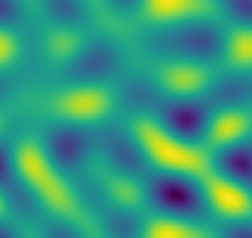
\includegraphics[interpolate=true,width=2.520000in,height=2.380000in]{burgers_forcing_0.01-img0.png}}%
\end{pgfscope}%
\begin{pgfscope}%
\pgfsetbuttcap%
\pgfsetroundjoin%
\definecolor{currentfill}{rgb}{0.000000,0.000000,0.000000}%
\pgfsetfillcolor{currentfill}%
\pgfsetlinewidth{0.803000pt}%
\definecolor{currentstroke}{rgb}{0.000000,0.000000,0.000000}%
\pgfsetstrokecolor{currentstroke}%
\pgfsetdash{}{0pt}%
\pgfsys@defobject{currentmarker}{\pgfqpoint{0.000000in}{-0.048611in}}{\pgfqpoint{0.000000in}{0.000000in}}{%
\pgfpathmoveto{\pgfqpoint{0.000000in}{0.000000in}}%
\pgfpathlineto{\pgfqpoint{0.000000in}{-0.048611in}}%
\pgfusepath{stroke,fill}%
}%
\begin{pgfscope}%
\pgfsys@transformshift{0.567820in}{0.517039in}%
\pgfsys@useobject{currentmarker}{}%
\end{pgfscope}%
\end{pgfscope}%
\begin{pgfscope}%
\definecolor{textcolor}{rgb}{0.000000,0.000000,0.000000}%
\pgfsetstrokecolor{textcolor}%
\pgfsetfillcolor{textcolor}%
\pgftext[x=0.567820in,y=0.419816in,,top]{\color{textcolor}\rmfamily\fontsize{12.000000}{14.400000}\selectfont 0.0}%
\end{pgfscope}%
\begin{pgfscope}%
\pgfsetbuttcap%
\pgfsetroundjoin%
\definecolor{currentfill}{rgb}{0.000000,0.000000,0.000000}%
\pgfsetfillcolor{currentfill}%
\pgfsetlinewidth{0.803000pt}%
\definecolor{currentstroke}{rgb}{0.000000,0.000000,0.000000}%
\pgfsetstrokecolor{currentstroke}%
\pgfsetdash{}{0pt}%
\pgfsys@defobject{currentmarker}{\pgfqpoint{0.000000in}{-0.048611in}}{\pgfqpoint{0.000000in}{0.000000in}}{%
\pgfpathmoveto{\pgfqpoint{0.000000in}{0.000000in}}%
\pgfpathlineto{\pgfqpoint{0.000000in}{-0.048611in}}%
\pgfusepath{stroke,fill}%
}%
\begin{pgfscope}%
\pgfsys@transformshift{1.196524in}{0.517039in}%
\pgfsys@useobject{currentmarker}{}%
\end{pgfscope}%
\end{pgfscope}%
\begin{pgfscope}%
\definecolor{textcolor}{rgb}{0.000000,0.000000,0.000000}%
\pgfsetstrokecolor{textcolor}%
\pgfsetfillcolor{textcolor}%
\pgftext[x=1.196524in,y=0.419816in,,top]{\color{textcolor}\rmfamily\fontsize{12.000000}{14.400000}\selectfont 0.5}%
\end{pgfscope}%
\begin{pgfscope}%
\pgfsetbuttcap%
\pgfsetroundjoin%
\definecolor{currentfill}{rgb}{0.000000,0.000000,0.000000}%
\pgfsetfillcolor{currentfill}%
\pgfsetlinewidth{0.803000pt}%
\definecolor{currentstroke}{rgb}{0.000000,0.000000,0.000000}%
\pgfsetstrokecolor{currentstroke}%
\pgfsetdash{}{0pt}%
\pgfsys@defobject{currentmarker}{\pgfqpoint{0.000000in}{-0.048611in}}{\pgfqpoint{0.000000in}{0.000000in}}{%
\pgfpathmoveto{\pgfqpoint{0.000000in}{0.000000in}}%
\pgfpathlineto{\pgfqpoint{0.000000in}{-0.048611in}}%
\pgfusepath{stroke,fill}%
}%
\begin{pgfscope}%
\pgfsys@transformshift{1.825229in}{0.517039in}%
\pgfsys@useobject{currentmarker}{}%
\end{pgfscope}%
\end{pgfscope}%
\begin{pgfscope}%
\definecolor{textcolor}{rgb}{0.000000,0.000000,0.000000}%
\pgfsetstrokecolor{textcolor}%
\pgfsetfillcolor{textcolor}%
\pgftext[x=1.825229in,y=0.419816in,,top]{\color{textcolor}\rmfamily\fontsize{12.000000}{14.400000}\selectfont 1.0}%
\end{pgfscope}%
\begin{pgfscope}%
\pgfsetbuttcap%
\pgfsetroundjoin%
\definecolor{currentfill}{rgb}{0.000000,0.000000,0.000000}%
\pgfsetfillcolor{currentfill}%
\pgfsetlinewidth{0.803000pt}%
\definecolor{currentstroke}{rgb}{0.000000,0.000000,0.000000}%
\pgfsetstrokecolor{currentstroke}%
\pgfsetdash{}{0pt}%
\pgfsys@defobject{currentmarker}{\pgfqpoint{0.000000in}{-0.048611in}}{\pgfqpoint{0.000000in}{0.000000in}}{%
\pgfpathmoveto{\pgfqpoint{0.000000in}{0.000000in}}%
\pgfpathlineto{\pgfqpoint{0.000000in}{-0.048611in}}%
\pgfusepath{stroke,fill}%
}%
\begin{pgfscope}%
\pgfsys@transformshift{2.453933in}{0.517039in}%
\pgfsys@useobject{currentmarker}{}%
\end{pgfscope}%
\end{pgfscope}%
\begin{pgfscope}%
\definecolor{textcolor}{rgb}{0.000000,0.000000,0.000000}%
\pgfsetstrokecolor{textcolor}%
\pgfsetfillcolor{textcolor}%
\pgftext[x=2.453933in,y=0.419816in,,top]{\color{textcolor}\rmfamily\fontsize{12.000000}{14.400000}\selectfont 1.5}%
\end{pgfscope}%
\begin{pgfscope}%
\pgfsetbuttcap%
\pgfsetroundjoin%
\definecolor{currentfill}{rgb}{0.000000,0.000000,0.000000}%
\pgfsetfillcolor{currentfill}%
\pgfsetlinewidth{0.803000pt}%
\definecolor{currentstroke}{rgb}{0.000000,0.000000,0.000000}%
\pgfsetstrokecolor{currentstroke}%
\pgfsetdash{}{0pt}%
\pgfsys@defobject{currentmarker}{\pgfqpoint{0.000000in}{-0.048611in}}{\pgfqpoint{0.000000in}{0.000000in}}{%
\pgfpathmoveto{\pgfqpoint{0.000000in}{0.000000in}}%
\pgfpathlineto{\pgfqpoint{0.000000in}{-0.048611in}}%
\pgfusepath{stroke,fill}%
}%
\begin{pgfscope}%
\pgfsys@transformshift{3.082637in}{0.517039in}%
\pgfsys@useobject{currentmarker}{}%
\end{pgfscope}%
\end{pgfscope}%
\begin{pgfscope}%
\definecolor{textcolor}{rgb}{0.000000,0.000000,0.000000}%
\pgfsetstrokecolor{textcolor}%
\pgfsetfillcolor{textcolor}%
\pgftext[x=3.082637in,y=0.419816in,,top]{\color{textcolor}\rmfamily\fontsize{12.000000}{14.400000}\selectfont 2.0}%
\end{pgfscope}%
\begin{pgfscope}%
\definecolor{textcolor}{rgb}{0.000000,0.000000,0.000000}%
\pgfsetstrokecolor{textcolor}%
\pgfsetfillcolor{textcolor}%
\pgftext[x=1.825229in,y=0.202965in,,top]{\color{textcolor}\rmfamily\fontsize{12.000000}{14.400000}\selectfont Space}%
\end{pgfscope}%
\begin{pgfscope}%
\pgfsetbuttcap%
\pgfsetroundjoin%
\definecolor{currentfill}{rgb}{0.000000,0.000000,0.000000}%
\pgfsetfillcolor{currentfill}%
\pgfsetlinewidth{0.803000pt}%
\definecolor{currentstroke}{rgb}{0.000000,0.000000,0.000000}%
\pgfsetstrokecolor{currentstroke}%
\pgfsetdash{}{0pt}%
\pgfsys@defobject{currentmarker}{\pgfqpoint{-0.048611in}{0.000000in}}{\pgfqpoint{-0.000000in}{0.000000in}}{%
\pgfpathmoveto{\pgfqpoint{-0.000000in}{0.000000in}}%
\pgfpathlineto{\pgfqpoint{-0.048611in}{0.000000in}}%
\pgfusepath{stroke,fill}%
}%
\begin{pgfscope}%
\pgfsys@transformshift{0.567820in}{0.517039in}%
\pgfsys@useobject{currentmarker}{}%
\end{pgfscope}%
\end{pgfscope}%
\begin{pgfscope}%
\definecolor{textcolor}{rgb}{0.000000,0.000000,0.000000}%
\pgfsetstrokecolor{textcolor}%
\pgfsetfillcolor{textcolor}%
\pgftext[x=0.364559in, y=0.453725in, left, base]{\color{textcolor}\rmfamily\fontsize{12.000000}{14.400000}\selectfont 0}%
\end{pgfscope}%
\begin{pgfscope}%
\pgfsetbuttcap%
\pgfsetroundjoin%
\definecolor{currentfill}{rgb}{0.000000,0.000000,0.000000}%
\pgfsetfillcolor{currentfill}%
\pgfsetlinewidth{0.803000pt}%
\definecolor{currentstroke}{rgb}{0.000000,0.000000,0.000000}%
\pgfsetstrokecolor{currentstroke}%
\pgfsetdash{}{0pt}%
\pgfsys@defobject{currentmarker}{\pgfqpoint{-0.048611in}{0.000000in}}{\pgfqpoint{-0.000000in}{0.000000in}}{%
\pgfpathmoveto{\pgfqpoint{-0.000000in}{0.000000in}}%
\pgfpathlineto{\pgfqpoint{-0.048611in}{0.000000in}}%
\pgfusepath{stroke,fill}%
}%
\begin{pgfscope}%
\pgfsys@transformshift{0.567820in}{0.992634in}%
\pgfsys@useobject{currentmarker}{}%
\end{pgfscope}%
\end{pgfscope}%
\begin{pgfscope}%
\definecolor{textcolor}{rgb}{0.000000,0.000000,0.000000}%
\pgfsetstrokecolor{textcolor}%
\pgfsetfillcolor{textcolor}%
\pgftext[x=0.364559in, y=0.929320in, left, base]{\color{textcolor}\rmfamily\fontsize{12.000000}{14.400000}\selectfont 2}%
\end{pgfscope}%
\begin{pgfscope}%
\pgfsetbuttcap%
\pgfsetroundjoin%
\definecolor{currentfill}{rgb}{0.000000,0.000000,0.000000}%
\pgfsetfillcolor{currentfill}%
\pgfsetlinewidth{0.803000pt}%
\definecolor{currentstroke}{rgb}{0.000000,0.000000,0.000000}%
\pgfsetstrokecolor{currentstroke}%
\pgfsetdash{}{0pt}%
\pgfsys@defobject{currentmarker}{\pgfqpoint{-0.048611in}{0.000000in}}{\pgfqpoint{-0.000000in}{0.000000in}}{%
\pgfpathmoveto{\pgfqpoint{-0.000000in}{0.000000in}}%
\pgfpathlineto{\pgfqpoint{-0.048611in}{0.000000in}}%
\pgfusepath{stroke,fill}%
}%
\begin{pgfscope}%
\pgfsys@transformshift{0.567820in}{1.468230in}%
\pgfsys@useobject{currentmarker}{}%
\end{pgfscope}%
\end{pgfscope}%
\begin{pgfscope}%
\definecolor{textcolor}{rgb}{0.000000,0.000000,0.000000}%
\pgfsetstrokecolor{textcolor}%
\pgfsetfillcolor{textcolor}%
\pgftext[x=0.364559in, y=1.404916in, left, base]{\color{textcolor}\rmfamily\fontsize{12.000000}{14.400000}\selectfont 4}%
\end{pgfscope}%
\begin{pgfscope}%
\pgfsetbuttcap%
\pgfsetroundjoin%
\definecolor{currentfill}{rgb}{0.000000,0.000000,0.000000}%
\pgfsetfillcolor{currentfill}%
\pgfsetlinewidth{0.803000pt}%
\definecolor{currentstroke}{rgb}{0.000000,0.000000,0.000000}%
\pgfsetstrokecolor{currentstroke}%
\pgfsetdash{}{0pt}%
\pgfsys@defobject{currentmarker}{\pgfqpoint{-0.048611in}{0.000000in}}{\pgfqpoint{-0.000000in}{0.000000in}}{%
\pgfpathmoveto{\pgfqpoint{-0.000000in}{0.000000in}}%
\pgfpathlineto{\pgfqpoint{-0.048611in}{0.000000in}}%
\pgfusepath{stroke,fill}%
}%
\begin{pgfscope}%
\pgfsys@transformshift{0.567820in}{1.943825in}%
\pgfsys@useobject{currentmarker}{}%
\end{pgfscope}%
\end{pgfscope}%
\begin{pgfscope}%
\definecolor{textcolor}{rgb}{0.000000,0.000000,0.000000}%
\pgfsetstrokecolor{textcolor}%
\pgfsetfillcolor{textcolor}%
\pgftext[x=0.364559in, y=1.880511in, left, base]{\color{textcolor}\rmfamily\fontsize{12.000000}{14.400000}\selectfont 6}%
\end{pgfscope}%
\begin{pgfscope}%
\pgfsetbuttcap%
\pgfsetroundjoin%
\definecolor{currentfill}{rgb}{0.000000,0.000000,0.000000}%
\pgfsetfillcolor{currentfill}%
\pgfsetlinewidth{0.803000pt}%
\definecolor{currentstroke}{rgb}{0.000000,0.000000,0.000000}%
\pgfsetstrokecolor{currentstroke}%
\pgfsetdash{}{0pt}%
\pgfsys@defobject{currentmarker}{\pgfqpoint{-0.048611in}{0.000000in}}{\pgfqpoint{-0.000000in}{0.000000in}}{%
\pgfpathmoveto{\pgfqpoint{-0.000000in}{0.000000in}}%
\pgfpathlineto{\pgfqpoint{-0.048611in}{0.000000in}}%
\pgfusepath{stroke,fill}%
}%
\begin{pgfscope}%
\pgfsys@transformshift{0.567820in}{2.419421in}%
\pgfsys@useobject{currentmarker}{}%
\end{pgfscope}%
\end{pgfscope}%
\begin{pgfscope}%
\definecolor{textcolor}{rgb}{0.000000,0.000000,0.000000}%
\pgfsetstrokecolor{textcolor}%
\pgfsetfillcolor{textcolor}%
\pgftext[x=0.364559in, y=2.356107in, left, base]{\color{textcolor}\rmfamily\fontsize{12.000000}{14.400000}\selectfont 8}%
\end{pgfscope}%
\begin{pgfscope}%
\pgfsetbuttcap%
\pgfsetroundjoin%
\definecolor{currentfill}{rgb}{0.000000,0.000000,0.000000}%
\pgfsetfillcolor{currentfill}%
\pgfsetlinewidth{0.803000pt}%
\definecolor{currentstroke}{rgb}{0.000000,0.000000,0.000000}%
\pgfsetstrokecolor{currentstroke}%
\pgfsetdash{}{0pt}%
\pgfsys@defobject{currentmarker}{\pgfqpoint{-0.048611in}{0.000000in}}{\pgfqpoint{-0.000000in}{0.000000in}}{%
\pgfpathmoveto{\pgfqpoint{-0.000000in}{0.000000in}}%
\pgfpathlineto{\pgfqpoint{-0.048611in}{0.000000in}}%
\pgfusepath{stroke,fill}%
}%
\begin{pgfscope}%
\pgfsys@transformshift{0.567820in}{2.895016in}%
\pgfsys@useobject{currentmarker}{}%
\end{pgfscope}%
\end{pgfscope}%
\begin{pgfscope}%
\definecolor{textcolor}{rgb}{0.000000,0.000000,0.000000}%
\pgfsetstrokecolor{textcolor}%
\pgfsetfillcolor{textcolor}%
\pgftext[x=0.258521in, y=2.831702in, left, base]{\color{textcolor}\rmfamily\fontsize{12.000000}{14.400000}\selectfont 10}%
\end{pgfscope}%
\begin{pgfscope}%
\definecolor{textcolor}{rgb}{0.000000,0.000000,0.000000}%
\pgfsetstrokecolor{textcolor}%
\pgfsetfillcolor{textcolor}%
\pgftext[x=0.202965in,y=1.706027in,,bottom,rotate=90.000000]{\color{textcolor}\rmfamily\fontsize{12.000000}{14.400000}\selectfont Time}%
\end{pgfscope}%
\begin{pgfscope}%
\pgfsetrectcap%
\pgfsetmiterjoin%
\pgfsetlinewidth{0.803000pt}%
\definecolor{currentstroke}{rgb}{0.000000,0.000000,0.000000}%
\pgfsetstrokecolor{currentstroke}%
\pgfsetdash{}{0pt}%
\pgfpathmoveto{\pgfqpoint{0.567820in}{0.517039in}}%
\pgfpathlineto{\pgfqpoint{0.567820in}{2.895016in}}%
\pgfusepath{stroke}%
\end{pgfscope}%
\begin{pgfscope}%
\pgfsetrectcap%
\pgfsetmiterjoin%
\pgfsetlinewidth{0.803000pt}%
\definecolor{currentstroke}{rgb}{0.000000,0.000000,0.000000}%
\pgfsetstrokecolor{currentstroke}%
\pgfsetdash{}{0pt}%
\pgfpathmoveto{\pgfqpoint{3.082637in}{0.517039in}}%
\pgfpathlineto{\pgfqpoint{3.082637in}{2.895016in}}%
\pgfusepath{stroke}%
\end{pgfscope}%
\begin{pgfscope}%
\pgfsetrectcap%
\pgfsetmiterjoin%
\pgfsetlinewidth{0.803000pt}%
\definecolor{currentstroke}{rgb}{0.000000,0.000000,0.000000}%
\pgfsetstrokecolor{currentstroke}%
\pgfsetdash{}{0pt}%
\pgfpathmoveto{\pgfqpoint{0.567820in}{0.517039in}}%
\pgfpathlineto{\pgfqpoint{3.082637in}{0.517039in}}%
\pgfusepath{stroke}%
\end{pgfscope}%
\begin{pgfscope}%
\pgfsetrectcap%
\pgfsetmiterjoin%
\pgfsetlinewidth{0.803000pt}%
\definecolor{currentstroke}{rgb}{0.000000,0.000000,0.000000}%
\pgfsetstrokecolor{currentstroke}%
\pgfsetdash{}{0pt}%
\pgfpathmoveto{\pgfqpoint{0.567820in}{2.895016in}}%
\pgfpathlineto{\pgfqpoint{3.082637in}{2.895016in}}%
\pgfusepath{stroke}%
\end{pgfscope}%
\begin{pgfscope}%
\pgfsetbuttcap%
\pgfsetmiterjoin%
\pgfsetlinewidth{0.000000pt}%
\definecolor{currentstroke}{rgb}{0.000000,0.000000,0.000000}%
\pgfsetstrokecolor{currentstroke}%
\pgfsetstrokeopacity{0.000000}%
\pgfsetdash{}{0pt}%
\pgfpathmoveto{\pgfqpoint{3.340906in}{0.517039in}}%
\pgfpathlineto{\pgfqpoint{3.459805in}{0.517039in}}%
\pgfpathlineto{\pgfqpoint{3.459805in}{2.895016in}}%
\pgfpathlineto{\pgfqpoint{3.340906in}{2.895016in}}%
\pgfpathlineto{\pgfqpoint{3.340906in}{0.517039in}}%
\pgfpathclose%
\pgfusepath{}%
\end{pgfscope}%
\begin{pgfscope}%
\pgfsys@transformshift{3.340000in}{0.520000in}%
\pgftext[left,bottom]{
\includegraphics[interpolate=true,width=0.120000in,height=2.380000in]{burgers_forcing_0.01-img1.png}}%
\end{pgfscope}%
\begin{pgfscope}%
\pgfsetbuttcap%
\pgfsetroundjoin%
\definecolor{currentfill}{rgb}{0.000000,0.000000,0.000000}%
\pgfsetfillcolor{currentfill}%
\pgfsetlinewidth{0.803000pt}%
\definecolor{currentstroke}{rgb}{0.000000,0.000000,0.000000}%
\pgfsetstrokecolor{currentstroke}%
\pgfsetdash{}{0pt}%
\pgfsys@defobject{currentmarker}{\pgfqpoint{0.000000in}{0.000000in}}{\pgfqpoint{0.048611in}{0.000000in}}{%
\pgfpathmoveto{\pgfqpoint{0.000000in}{0.000000in}}%
\pgfpathlineto{\pgfqpoint{0.048611in}{0.000000in}}%
\pgfusepath{stroke,fill}%
}%
\begin{pgfscope}%
\pgfsys@transformshift{3.459805in}{0.686748in}%
\pgfsys@useobject{currentmarker}{}%
\end{pgfscope}%
\end{pgfscope}%
\begin{pgfscope}%
\definecolor{textcolor}{rgb}{0.000000,0.000000,0.000000}%
\pgfsetstrokecolor{textcolor}%
\pgfsetfillcolor{textcolor}%
\pgftext[x=3.557027in, y=0.623435in, left, base]{\color{textcolor}\rmfamily\fontsize{12.000000}{14.400000}\selectfont \ensuremath{-}1.0}%
\end{pgfscope}%
\begin{pgfscope}%
\pgfsetbuttcap%
\pgfsetroundjoin%
\definecolor{currentfill}{rgb}{0.000000,0.000000,0.000000}%
\pgfsetfillcolor{currentfill}%
\pgfsetlinewidth{0.803000pt}%
\definecolor{currentstroke}{rgb}{0.000000,0.000000,0.000000}%
\pgfsetstrokecolor{currentstroke}%
\pgfsetdash{}{0pt}%
\pgfsys@defobject{currentmarker}{\pgfqpoint{0.000000in}{0.000000in}}{\pgfqpoint{0.048611in}{0.000000in}}{%
\pgfpathmoveto{\pgfqpoint{0.000000in}{0.000000in}}%
\pgfpathlineto{\pgfqpoint{0.048611in}{0.000000in}}%
\pgfusepath{stroke,fill}%
}%
\begin{pgfscope}%
\pgfsys@transformshift{3.459805in}{1.263230in}%
\pgfsys@useobject{currentmarker}{}%
\end{pgfscope}%
\end{pgfscope}%
\begin{pgfscope}%
\definecolor{textcolor}{rgb}{0.000000,0.000000,0.000000}%
\pgfsetstrokecolor{textcolor}%
\pgfsetfillcolor{textcolor}%
\pgftext[x=3.557027in, y=1.199916in, left, base]{\color{textcolor}\rmfamily\fontsize{12.000000}{14.400000}\selectfont \ensuremath{-}0.5}%
\end{pgfscope}%
\begin{pgfscope}%
\pgfsetbuttcap%
\pgfsetroundjoin%
\definecolor{currentfill}{rgb}{0.000000,0.000000,0.000000}%
\pgfsetfillcolor{currentfill}%
\pgfsetlinewidth{0.803000pt}%
\definecolor{currentstroke}{rgb}{0.000000,0.000000,0.000000}%
\pgfsetstrokecolor{currentstroke}%
\pgfsetdash{}{0pt}%
\pgfsys@defobject{currentmarker}{\pgfqpoint{0.000000in}{0.000000in}}{\pgfqpoint{0.048611in}{0.000000in}}{%
\pgfpathmoveto{\pgfqpoint{0.000000in}{0.000000in}}%
\pgfpathlineto{\pgfqpoint{0.048611in}{0.000000in}}%
\pgfusepath{stroke,fill}%
}%
\begin{pgfscope}%
\pgfsys@transformshift{3.459805in}{1.839712in}%
\pgfsys@useobject{currentmarker}{}%
\end{pgfscope}%
\end{pgfscope}%
\begin{pgfscope}%
\definecolor{textcolor}{rgb}{0.000000,0.000000,0.000000}%
\pgfsetstrokecolor{textcolor}%
\pgfsetfillcolor{textcolor}%
\pgftext[x=3.557027in, y=1.776398in, left, base]{\color{textcolor}\rmfamily\fontsize{12.000000}{14.400000}\selectfont 0.0}%
\end{pgfscope}%
\begin{pgfscope}%
\pgfsetbuttcap%
\pgfsetroundjoin%
\definecolor{currentfill}{rgb}{0.000000,0.000000,0.000000}%
\pgfsetfillcolor{currentfill}%
\pgfsetlinewidth{0.803000pt}%
\definecolor{currentstroke}{rgb}{0.000000,0.000000,0.000000}%
\pgfsetstrokecolor{currentstroke}%
\pgfsetdash{}{0pt}%
\pgfsys@defobject{currentmarker}{\pgfqpoint{0.000000in}{0.000000in}}{\pgfqpoint{0.048611in}{0.000000in}}{%
\pgfpathmoveto{\pgfqpoint{0.000000in}{0.000000in}}%
\pgfpathlineto{\pgfqpoint{0.048611in}{0.000000in}}%
\pgfusepath{stroke,fill}%
}%
\begin{pgfscope}%
\pgfsys@transformshift{3.459805in}{2.416193in}%
\pgfsys@useobject{currentmarker}{}%
\end{pgfscope}%
\end{pgfscope}%
\begin{pgfscope}%
\definecolor{textcolor}{rgb}{0.000000,0.000000,0.000000}%
\pgfsetstrokecolor{textcolor}%
\pgfsetfillcolor{textcolor}%
\pgftext[x=3.557027in, y=2.352879in, left, base]{\color{textcolor}\rmfamily\fontsize{12.000000}{14.400000}\selectfont 0.5}%
\end{pgfscope}%
\begin{pgfscope}%
\pgfsetrectcap%
\pgfsetmiterjoin%
\pgfsetlinewidth{0.803000pt}%
\definecolor{currentstroke}{rgb}{0.000000,0.000000,0.000000}%
\pgfsetstrokecolor{currentstroke}%
\pgfsetdash{}{0pt}%
\pgfpathmoveto{\pgfqpoint{3.340906in}{0.517039in}}%
\pgfpathlineto{\pgfqpoint{3.400355in}{0.517039in}}%
\pgfpathlineto{\pgfqpoint{3.459805in}{0.517039in}}%
\pgfpathlineto{\pgfqpoint{3.459805in}{2.895016in}}%
\pgfpathlineto{\pgfqpoint{3.400355in}{2.895016in}}%
\pgfpathlineto{\pgfqpoint{3.340906in}{2.895016in}}%
\pgfpathlineto{\pgfqpoint{3.340906in}{0.517039in}}%
\pgfpathclose%
\pgfusepath{stroke}%
\end{pgfscope}%
\end{pgfpicture}%
\makeatother%
\endgroup%

    \end{adjustbox}
    \caption{Forcing function for \(\nu=0.01\).}\label{fig:burgers_forcing_0.01}
  \end{subfigure}
  % \\[-0.7\baselineskip]
  \begin{subfigure}{0.49\linewidth}
    \begin{adjustbox}{width=\linewidth}
      \begingroup%
\makeatletter%
\begin{pgfpicture}%
\pgfpathrectangle{\pgfpointorigin}{\pgfqpoint{4.000000in}{3.000000in}}%
\pgfusepath{use as bounding box, clip}%
\begin{pgfscope}%
\pgfsetbuttcap%
\pgfsetmiterjoin%
\pgfsetlinewidth{0.000000pt}%
\definecolor{currentstroke}{rgb}{0.000000,0.000000,0.000000}%
\pgfsetstrokecolor{currentstroke}%
\pgfsetstrokeopacity{0.000000}%
\pgfsetdash{}{0pt}%
\pgfpathmoveto{\pgfqpoint{0.000000in}{0.000000in}}%
\pgfpathlineto{\pgfqpoint{4.000000in}{0.000000in}}%
\pgfpathlineto{\pgfqpoint{4.000000in}{3.000000in}}%
\pgfpathlineto{\pgfqpoint{0.000000in}{3.000000in}}%
\pgfpathlineto{\pgfqpoint{0.000000in}{0.000000in}}%
\pgfpathclose%
\pgfusepath{}%
\end{pgfscope}%
\begin{pgfscope}%
\pgfsetbuttcap%
\pgfsetmiterjoin%
\pgfsetlinewidth{0.000000pt}%
\definecolor{currentstroke}{rgb}{0.000000,0.000000,0.000000}%
\pgfsetstrokecolor{currentstroke}%
\pgfsetstrokeopacity{0.000000}%
\pgfsetdash{}{0pt}%
\pgfpathmoveto{\pgfqpoint{0.350969in}{0.300188in}}%
\pgfpathlineto{\pgfqpoint{3.061494in}{0.300188in}}%
\pgfpathlineto{\pgfqpoint{3.061494in}{2.895016in}}%
\pgfpathlineto{\pgfqpoint{0.350969in}{2.895016in}}%
\pgfpathlineto{\pgfqpoint{0.350969in}{0.300188in}}%
\pgfpathclose%
\pgfusepath{}%
\end{pgfscope}%
\begin{pgfscope}%
\pgfpathrectangle{\pgfqpoint{0.350969in}{0.300188in}}{\pgfqpoint{2.710525in}{2.594829in}}%
\pgfusepath{clip}%
\pgfsys@transformshift{0.350969in}{0.300188in}%
\pgftext[left,bottom]{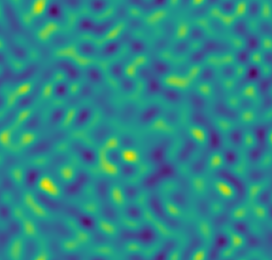
\includegraphics[interpolate=true,width=2.720000in,height=2.600000in]{burgers_solution_0.1-img0.png}}%
\end{pgfscope}%
\begin{pgfscope}%
\pgfsetbuttcap%
\pgfsetroundjoin%
\definecolor{currentfill}{rgb}{0.000000,0.000000,0.000000}%
\pgfsetfillcolor{currentfill}%
\pgfsetlinewidth{0.803000pt}%
\definecolor{currentstroke}{rgb}{0.000000,0.000000,0.000000}%
\pgfsetstrokecolor{currentstroke}%
\pgfsetdash{}{0pt}%
\pgfsys@defobject{currentmarker}{\pgfqpoint{0.000000in}{-0.048611in}}{\pgfqpoint{0.000000in}{0.000000in}}{%
\pgfpathmoveto{\pgfqpoint{0.000000in}{0.000000in}}%
\pgfpathlineto{\pgfqpoint{0.000000in}{-0.048611in}}%
\pgfusepath{stroke,fill}%
}%
\begin{pgfscope}%
\pgfsys@transformshift{0.350969in}{0.300188in}%
\pgfsys@useobject{currentmarker}{}%
\end{pgfscope}%
\end{pgfscope}%
\begin{pgfscope}%
\definecolor{textcolor}{rgb}{0.000000,0.000000,0.000000}%
\pgfsetstrokecolor{textcolor}%
\pgfsetfillcolor{textcolor}%
\pgftext[x=0.350969in,y=0.202965in,,top]{\color{textcolor}{\rmfamily\fontsize{12.000000}{14.400000}\selectfont\catcode`\^=\active\def^{\ifmmode\sp\else\^{}\fi}\catcode`\%=\active\def%{\%}0.0}}%
\end{pgfscope}%
\begin{pgfscope}%
\pgfsetbuttcap%
\pgfsetroundjoin%
\definecolor{currentfill}{rgb}{0.000000,0.000000,0.000000}%
\pgfsetfillcolor{currentfill}%
\pgfsetlinewidth{0.803000pt}%
\definecolor{currentstroke}{rgb}{0.000000,0.000000,0.000000}%
\pgfsetstrokecolor{currentstroke}%
\pgfsetdash{}{0pt}%
\pgfsys@defobject{currentmarker}{\pgfqpoint{0.000000in}{-0.048611in}}{\pgfqpoint{0.000000in}{0.000000in}}{%
\pgfpathmoveto{\pgfqpoint{0.000000in}{0.000000in}}%
\pgfpathlineto{\pgfqpoint{0.000000in}{-0.048611in}}%
\pgfusepath{stroke,fill}%
}%
\begin{pgfscope}%
\pgfsys@transformshift{1.028600in}{0.300188in}%
\pgfsys@useobject{currentmarker}{}%
\end{pgfscope}%
\end{pgfscope}%
\begin{pgfscope}%
\definecolor{textcolor}{rgb}{0.000000,0.000000,0.000000}%
\pgfsetstrokecolor{textcolor}%
\pgfsetfillcolor{textcolor}%
\pgftext[x=1.028600in,y=0.202965in,,top]{\color{textcolor}{\rmfamily\fontsize{12.000000}{14.400000}\selectfont\catcode`\^=\active\def^{\ifmmode\sp\else\^{}\fi}\catcode`\%=\active\def%{\%}0.5}}%
\end{pgfscope}%
\begin{pgfscope}%
\pgfsetbuttcap%
\pgfsetroundjoin%
\definecolor{currentfill}{rgb}{0.000000,0.000000,0.000000}%
\pgfsetfillcolor{currentfill}%
\pgfsetlinewidth{0.803000pt}%
\definecolor{currentstroke}{rgb}{0.000000,0.000000,0.000000}%
\pgfsetstrokecolor{currentstroke}%
\pgfsetdash{}{0pt}%
\pgfsys@defobject{currentmarker}{\pgfqpoint{0.000000in}{-0.048611in}}{\pgfqpoint{0.000000in}{0.000000in}}{%
\pgfpathmoveto{\pgfqpoint{0.000000in}{0.000000in}}%
\pgfpathlineto{\pgfqpoint{0.000000in}{-0.048611in}}%
\pgfusepath{stroke,fill}%
}%
\begin{pgfscope}%
\pgfsys@transformshift{1.706232in}{0.300188in}%
\pgfsys@useobject{currentmarker}{}%
\end{pgfscope}%
\end{pgfscope}%
\begin{pgfscope}%
\definecolor{textcolor}{rgb}{0.000000,0.000000,0.000000}%
\pgfsetstrokecolor{textcolor}%
\pgfsetfillcolor{textcolor}%
\pgftext[x=1.706232in,y=0.202965in,,top]{\color{textcolor}{\rmfamily\fontsize{12.000000}{14.400000}\selectfont\catcode`\^=\active\def^{\ifmmode\sp\else\^{}\fi}\catcode`\%=\active\def%{\%}1.0}}%
\end{pgfscope}%
\begin{pgfscope}%
\pgfsetbuttcap%
\pgfsetroundjoin%
\definecolor{currentfill}{rgb}{0.000000,0.000000,0.000000}%
\pgfsetfillcolor{currentfill}%
\pgfsetlinewidth{0.803000pt}%
\definecolor{currentstroke}{rgb}{0.000000,0.000000,0.000000}%
\pgfsetstrokecolor{currentstroke}%
\pgfsetdash{}{0pt}%
\pgfsys@defobject{currentmarker}{\pgfqpoint{0.000000in}{-0.048611in}}{\pgfqpoint{0.000000in}{0.000000in}}{%
\pgfpathmoveto{\pgfqpoint{0.000000in}{0.000000in}}%
\pgfpathlineto{\pgfqpoint{0.000000in}{-0.048611in}}%
\pgfusepath{stroke,fill}%
}%
\begin{pgfscope}%
\pgfsys@transformshift{2.383863in}{0.300188in}%
\pgfsys@useobject{currentmarker}{}%
\end{pgfscope}%
\end{pgfscope}%
\begin{pgfscope}%
\definecolor{textcolor}{rgb}{0.000000,0.000000,0.000000}%
\pgfsetstrokecolor{textcolor}%
\pgfsetfillcolor{textcolor}%
\pgftext[x=2.383863in,y=0.202965in,,top]{\color{textcolor}{\rmfamily\fontsize{12.000000}{14.400000}\selectfont\catcode`\^=\active\def^{\ifmmode\sp\else\^{}\fi}\catcode`\%=\active\def%{\%}1.5}}%
\end{pgfscope}%
\begin{pgfscope}%
\pgfsetbuttcap%
\pgfsetroundjoin%
\definecolor{currentfill}{rgb}{0.000000,0.000000,0.000000}%
\pgfsetfillcolor{currentfill}%
\pgfsetlinewidth{0.803000pt}%
\definecolor{currentstroke}{rgb}{0.000000,0.000000,0.000000}%
\pgfsetstrokecolor{currentstroke}%
\pgfsetdash{}{0pt}%
\pgfsys@defobject{currentmarker}{\pgfqpoint{0.000000in}{-0.048611in}}{\pgfqpoint{0.000000in}{0.000000in}}{%
\pgfpathmoveto{\pgfqpoint{0.000000in}{0.000000in}}%
\pgfpathlineto{\pgfqpoint{0.000000in}{-0.048611in}}%
\pgfusepath{stroke,fill}%
}%
\begin{pgfscope}%
\pgfsys@transformshift{3.061494in}{0.300188in}%
\pgfsys@useobject{currentmarker}{}%
\end{pgfscope}%
\end{pgfscope}%
\begin{pgfscope}%
\definecolor{textcolor}{rgb}{0.000000,0.000000,0.000000}%
\pgfsetstrokecolor{textcolor}%
\pgfsetfillcolor{textcolor}%
\pgftext[x=3.061494in,y=0.202965in,,top]{\color{textcolor}{\rmfamily\fontsize{12.000000}{14.400000}\selectfont\catcode`\^=\active\def^{\ifmmode\sp\else\^{}\fi}\catcode`\%=\active\def%{\%}2.0}}%
\end{pgfscope}%
\begin{pgfscope}%
\pgfsetbuttcap%
\pgfsetroundjoin%
\definecolor{currentfill}{rgb}{0.000000,0.000000,0.000000}%
\pgfsetfillcolor{currentfill}%
\pgfsetlinewidth{0.803000pt}%
\definecolor{currentstroke}{rgb}{0.000000,0.000000,0.000000}%
\pgfsetstrokecolor{currentstroke}%
\pgfsetdash{}{0pt}%
\pgfsys@defobject{currentmarker}{\pgfqpoint{-0.048611in}{0.000000in}}{\pgfqpoint{-0.000000in}{0.000000in}}{%
\pgfpathmoveto{\pgfqpoint{-0.000000in}{0.000000in}}%
\pgfpathlineto{\pgfqpoint{-0.048611in}{0.000000in}}%
\pgfusepath{stroke,fill}%
}%
\begin{pgfscope}%
\pgfsys@transformshift{0.350969in}{0.300188in}%
\pgfsys@useobject{currentmarker}{}%
\end{pgfscope}%
\end{pgfscope}%
\begin{pgfscope}%
\definecolor{textcolor}{rgb}{0.000000,0.000000,0.000000}%
\pgfsetstrokecolor{textcolor}%
\pgfsetfillcolor{textcolor}%
\pgftext[x=0.147708in, y=0.236874in, left, base]{\color{textcolor}{\rmfamily\fontsize{12.000000}{14.400000}\selectfont\catcode`\^=\active\def^{\ifmmode\sp\else\^{}\fi}\catcode`\%=\active\def%{\%}0}}%
\end{pgfscope}%
\begin{pgfscope}%
\pgfsetbuttcap%
\pgfsetroundjoin%
\definecolor{currentfill}{rgb}{0.000000,0.000000,0.000000}%
\pgfsetfillcolor{currentfill}%
\pgfsetlinewidth{0.803000pt}%
\definecolor{currentstroke}{rgb}{0.000000,0.000000,0.000000}%
\pgfsetstrokecolor{currentstroke}%
\pgfsetdash{}{0pt}%
\pgfsys@defobject{currentmarker}{\pgfqpoint{-0.048611in}{0.000000in}}{\pgfqpoint{-0.000000in}{0.000000in}}{%
\pgfpathmoveto{\pgfqpoint{-0.000000in}{0.000000in}}%
\pgfpathlineto{\pgfqpoint{-0.048611in}{0.000000in}}%
\pgfusepath{stroke,fill}%
}%
\begin{pgfscope}%
\pgfsys@transformshift{0.350969in}{0.819153in}%
\pgfsys@useobject{currentmarker}{}%
\end{pgfscope}%
\end{pgfscope}%
\begin{pgfscope}%
\definecolor{textcolor}{rgb}{0.000000,0.000000,0.000000}%
\pgfsetstrokecolor{textcolor}%
\pgfsetfillcolor{textcolor}%
\pgftext[x=0.147708in, y=0.755840in, left, base]{\color{textcolor}{\rmfamily\fontsize{12.000000}{14.400000}\selectfont\catcode`\^=\active\def^{\ifmmode\sp\else\^{}\fi}\catcode`\%=\active\def%{\%}2}}%
\end{pgfscope}%
\begin{pgfscope}%
\pgfsetbuttcap%
\pgfsetroundjoin%
\definecolor{currentfill}{rgb}{0.000000,0.000000,0.000000}%
\pgfsetfillcolor{currentfill}%
\pgfsetlinewidth{0.803000pt}%
\definecolor{currentstroke}{rgb}{0.000000,0.000000,0.000000}%
\pgfsetstrokecolor{currentstroke}%
\pgfsetdash{}{0pt}%
\pgfsys@defobject{currentmarker}{\pgfqpoint{-0.048611in}{0.000000in}}{\pgfqpoint{-0.000000in}{0.000000in}}{%
\pgfpathmoveto{\pgfqpoint{-0.000000in}{0.000000in}}%
\pgfpathlineto{\pgfqpoint{-0.048611in}{0.000000in}}%
\pgfusepath{stroke,fill}%
}%
\begin{pgfscope}%
\pgfsys@transformshift{0.350969in}{1.338119in}%
\pgfsys@useobject{currentmarker}{}%
\end{pgfscope}%
\end{pgfscope}%
\begin{pgfscope}%
\definecolor{textcolor}{rgb}{0.000000,0.000000,0.000000}%
\pgfsetstrokecolor{textcolor}%
\pgfsetfillcolor{textcolor}%
\pgftext[x=0.147708in, y=1.274805in, left, base]{\color{textcolor}{\rmfamily\fontsize{12.000000}{14.400000}\selectfont\catcode`\^=\active\def^{\ifmmode\sp\else\^{}\fi}\catcode`\%=\active\def%{\%}4}}%
\end{pgfscope}%
\begin{pgfscope}%
\pgfsetbuttcap%
\pgfsetroundjoin%
\definecolor{currentfill}{rgb}{0.000000,0.000000,0.000000}%
\pgfsetfillcolor{currentfill}%
\pgfsetlinewidth{0.803000pt}%
\definecolor{currentstroke}{rgb}{0.000000,0.000000,0.000000}%
\pgfsetstrokecolor{currentstroke}%
\pgfsetdash{}{0pt}%
\pgfsys@defobject{currentmarker}{\pgfqpoint{-0.048611in}{0.000000in}}{\pgfqpoint{-0.000000in}{0.000000in}}{%
\pgfpathmoveto{\pgfqpoint{-0.000000in}{0.000000in}}%
\pgfpathlineto{\pgfqpoint{-0.048611in}{0.000000in}}%
\pgfusepath{stroke,fill}%
}%
\begin{pgfscope}%
\pgfsys@transformshift{0.350969in}{1.857085in}%
\pgfsys@useobject{currentmarker}{}%
\end{pgfscope}%
\end{pgfscope}%
\begin{pgfscope}%
\definecolor{textcolor}{rgb}{0.000000,0.000000,0.000000}%
\pgfsetstrokecolor{textcolor}%
\pgfsetfillcolor{textcolor}%
\pgftext[x=0.147708in, y=1.793771in, left, base]{\color{textcolor}{\rmfamily\fontsize{12.000000}{14.400000}\selectfont\catcode`\^=\active\def^{\ifmmode\sp\else\^{}\fi}\catcode`\%=\active\def%{\%}6}}%
\end{pgfscope}%
\begin{pgfscope}%
\pgfsetbuttcap%
\pgfsetroundjoin%
\definecolor{currentfill}{rgb}{0.000000,0.000000,0.000000}%
\pgfsetfillcolor{currentfill}%
\pgfsetlinewidth{0.803000pt}%
\definecolor{currentstroke}{rgb}{0.000000,0.000000,0.000000}%
\pgfsetstrokecolor{currentstroke}%
\pgfsetdash{}{0pt}%
\pgfsys@defobject{currentmarker}{\pgfqpoint{-0.048611in}{0.000000in}}{\pgfqpoint{-0.000000in}{0.000000in}}{%
\pgfpathmoveto{\pgfqpoint{-0.000000in}{0.000000in}}%
\pgfpathlineto{\pgfqpoint{-0.048611in}{0.000000in}}%
\pgfusepath{stroke,fill}%
}%
\begin{pgfscope}%
\pgfsys@transformshift{0.350969in}{2.376050in}%
\pgfsys@useobject{currentmarker}{}%
\end{pgfscope}%
\end{pgfscope}%
\begin{pgfscope}%
\definecolor{textcolor}{rgb}{0.000000,0.000000,0.000000}%
\pgfsetstrokecolor{textcolor}%
\pgfsetfillcolor{textcolor}%
\pgftext[x=0.147708in, y=2.312737in, left, base]{\color{textcolor}{\rmfamily\fontsize{12.000000}{14.400000}\selectfont\catcode`\^=\active\def^{\ifmmode\sp\else\^{}\fi}\catcode`\%=\active\def%{\%}8}}%
\end{pgfscope}%
\begin{pgfscope}%
\pgfsetbuttcap%
\pgfsetroundjoin%
\definecolor{currentfill}{rgb}{0.000000,0.000000,0.000000}%
\pgfsetfillcolor{currentfill}%
\pgfsetlinewidth{0.803000pt}%
\definecolor{currentstroke}{rgb}{0.000000,0.000000,0.000000}%
\pgfsetstrokecolor{currentstroke}%
\pgfsetdash{}{0pt}%
\pgfsys@defobject{currentmarker}{\pgfqpoint{-0.048611in}{0.000000in}}{\pgfqpoint{-0.000000in}{0.000000in}}{%
\pgfpathmoveto{\pgfqpoint{-0.000000in}{0.000000in}}%
\pgfpathlineto{\pgfqpoint{-0.048611in}{0.000000in}}%
\pgfusepath{stroke,fill}%
}%
\begin{pgfscope}%
\pgfsys@transformshift{0.350969in}{2.895016in}%
\pgfsys@useobject{currentmarker}{}%
\end{pgfscope}%
\end{pgfscope}%
\begin{pgfscope}%
\definecolor{textcolor}{rgb}{0.000000,0.000000,0.000000}%
\pgfsetstrokecolor{textcolor}%
\pgfsetfillcolor{textcolor}%
\pgftext[x=0.041670in, y=2.831702in, left, base]{\color{textcolor}{\rmfamily\fontsize{12.000000}{14.400000}\selectfont\catcode`\^=\active\def^{\ifmmode\sp\else\^{}\fi}\catcode`\%=\active\def%{\%}10}}%
\end{pgfscope}%
\begin{pgfscope}%
\pgfsetrectcap%
\pgfsetmiterjoin%
\pgfsetlinewidth{0.803000pt}%
\definecolor{currentstroke}{rgb}{0.000000,0.000000,0.000000}%
\pgfsetstrokecolor{currentstroke}%
\pgfsetdash{}{0pt}%
\pgfpathmoveto{\pgfqpoint{0.350969in}{0.300188in}}%
\pgfpathlineto{\pgfqpoint{0.350969in}{2.895016in}}%
\pgfusepath{stroke}%
\end{pgfscope}%
\begin{pgfscope}%
\pgfsetrectcap%
\pgfsetmiterjoin%
\pgfsetlinewidth{0.803000pt}%
\definecolor{currentstroke}{rgb}{0.000000,0.000000,0.000000}%
\pgfsetstrokecolor{currentstroke}%
\pgfsetdash{}{0pt}%
\pgfpathmoveto{\pgfqpoint{3.061494in}{0.300188in}}%
\pgfpathlineto{\pgfqpoint{3.061494in}{2.895016in}}%
\pgfusepath{stroke}%
\end{pgfscope}%
\begin{pgfscope}%
\pgfsetrectcap%
\pgfsetmiterjoin%
\pgfsetlinewidth{0.803000pt}%
\definecolor{currentstroke}{rgb}{0.000000,0.000000,0.000000}%
\pgfsetstrokecolor{currentstroke}%
\pgfsetdash{}{0pt}%
\pgfpathmoveto{\pgfqpoint{0.350969in}{0.300188in}}%
\pgfpathlineto{\pgfqpoint{3.061494in}{0.300188in}}%
\pgfusepath{stroke}%
\end{pgfscope}%
\begin{pgfscope}%
\pgfsetrectcap%
\pgfsetmiterjoin%
\pgfsetlinewidth{0.803000pt}%
\definecolor{currentstroke}{rgb}{0.000000,0.000000,0.000000}%
\pgfsetstrokecolor{currentstroke}%
\pgfsetdash{}{0pt}%
\pgfpathmoveto{\pgfqpoint{0.350969in}{2.895016in}}%
\pgfpathlineto{\pgfqpoint{3.061494in}{2.895016in}}%
\pgfusepath{stroke}%
\end{pgfscope}%
\begin{pgfscope}%
\pgfsetbuttcap%
\pgfsetmiterjoin%
\pgfsetlinewidth{0.000000pt}%
\definecolor{currentstroke}{rgb}{0.000000,0.000000,0.000000}%
\pgfsetstrokecolor{currentstroke}%
\pgfsetstrokeopacity{0.000000}%
\pgfsetdash{}{0pt}%
\pgfpathmoveto{\pgfqpoint{3.329548in}{0.300188in}}%
\pgfpathlineto{\pgfqpoint{3.459290in}{0.300188in}}%
\pgfpathlineto{\pgfqpoint{3.459290in}{2.895016in}}%
\pgfpathlineto{\pgfqpoint{3.329548in}{2.895016in}}%
\pgfpathlineto{\pgfqpoint{3.329548in}{0.300188in}}%
\pgfpathclose%
\pgfusepath{}%
\end{pgfscope}%
\begin{pgfscope}%
\pgfsys@transformshift{3.330000in}{0.300000in}%
\pgftext[left,bottom]{
\includegraphics[interpolate=true,width=0.130000in,height=2.600000in]{burgers_solution_0.1-img1.png}}%
\end{pgfscope}%
\begin{pgfscope}%
\pgfsetbuttcap%
\pgfsetroundjoin%
\definecolor{currentfill}{rgb}{0.000000,0.000000,0.000000}%
\pgfsetfillcolor{currentfill}%
\pgfsetlinewidth{0.803000pt}%
\definecolor{currentstroke}{rgb}{0.000000,0.000000,0.000000}%
\pgfsetstrokecolor{currentstroke}%
\pgfsetdash{}{0pt}%
\pgfsys@defobject{currentmarker}{\pgfqpoint{0.000000in}{0.000000in}}{\pgfqpoint{0.048611in}{0.000000in}}{%
\pgfpathmoveto{\pgfqpoint{0.000000in}{0.000000in}}%
\pgfpathlineto{\pgfqpoint{0.048611in}{0.000000in}}%
\pgfusepath{stroke,fill}%
}%
\begin{pgfscope}%
\pgfsys@transformshift{3.459290in}{0.840201in}%
\pgfsys@useobject{currentmarker}{}%
\end{pgfscope}%
\end{pgfscope}%
\begin{pgfscope}%
\definecolor{textcolor}{rgb}{0.000000,0.000000,0.000000}%
\pgfsetstrokecolor{textcolor}%
\pgfsetfillcolor{textcolor}%
\pgftext[x=3.556512in, y=0.776887in, left, base]{\color{textcolor}{\rmfamily\fontsize{12.000000}{14.400000}\selectfont\catcode`\^=\active\def^{\ifmmode\sp\else\^{}\fi}\catcode`\%=\active\def%{\%}\ensuremath{-}0.5}}%
\end{pgfscope}%
\begin{pgfscope}%
\pgfsetbuttcap%
\pgfsetroundjoin%
\definecolor{currentfill}{rgb}{0.000000,0.000000,0.000000}%
\pgfsetfillcolor{currentfill}%
\pgfsetlinewidth{0.803000pt}%
\definecolor{currentstroke}{rgb}{0.000000,0.000000,0.000000}%
\pgfsetstrokecolor{currentstroke}%
\pgfsetdash{}{0pt}%
\pgfsys@defobject{currentmarker}{\pgfqpoint{0.000000in}{0.000000in}}{\pgfqpoint{0.048611in}{0.000000in}}{%
\pgfpathmoveto{\pgfqpoint{0.000000in}{0.000000in}}%
\pgfpathlineto{\pgfqpoint{0.048611in}{0.000000in}}%
\pgfusepath{stroke,fill}%
}%
\begin{pgfscope}%
\pgfsys@transformshift{3.459290in}{1.494629in}%
\pgfsys@useobject{currentmarker}{}%
\end{pgfscope}%
\end{pgfscope}%
\begin{pgfscope}%
\definecolor{textcolor}{rgb}{0.000000,0.000000,0.000000}%
\pgfsetstrokecolor{textcolor}%
\pgfsetfillcolor{textcolor}%
\pgftext[x=3.556512in, y=1.431315in, left, base]{\color{textcolor}{\rmfamily\fontsize{12.000000}{14.400000}\selectfont\catcode`\^=\active\def^{\ifmmode\sp\else\^{}\fi}\catcode`\%=\active\def%{\%}0.0}}%
\end{pgfscope}%
\begin{pgfscope}%
\pgfsetbuttcap%
\pgfsetroundjoin%
\definecolor{currentfill}{rgb}{0.000000,0.000000,0.000000}%
\pgfsetfillcolor{currentfill}%
\pgfsetlinewidth{0.803000pt}%
\definecolor{currentstroke}{rgb}{0.000000,0.000000,0.000000}%
\pgfsetstrokecolor{currentstroke}%
\pgfsetdash{}{0pt}%
\pgfsys@defobject{currentmarker}{\pgfqpoint{0.000000in}{0.000000in}}{\pgfqpoint{0.048611in}{0.000000in}}{%
\pgfpathmoveto{\pgfqpoint{0.000000in}{0.000000in}}%
\pgfpathlineto{\pgfqpoint{0.048611in}{0.000000in}}%
\pgfusepath{stroke,fill}%
}%
\begin{pgfscope}%
\pgfsys@transformshift{3.459290in}{2.149056in}%
\pgfsys@useobject{currentmarker}{}%
\end{pgfscope}%
\end{pgfscope}%
\begin{pgfscope}%
\definecolor{textcolor}{rgb}{0.000000,0.000000,0.000000}%
\pgfsetstrokecolor{textcolor}%
\pgfsetfillcolor{textcolor}%
\pgftext[x=3.556512in, y=2.085742in, left, base]{\color{textcolor}{\rmfamily\fontsize{12.000000}{14.400000}\selectfont\catcode`\^=\active\def^{\ifmmode\sp\else\^{}\fi}\catcode`\%=\active\def%{\%}0.5}}%
\end{pgfscope}%
\begin{pgfscope}%
\pgfsetbuttcap%
\pgfsetroundjoin%
\definecolor{currentfill}{rgb}{0.000000,0.000000,0.000000}%
\pgfsetfillcolor{currentfill}%
\pgfsetlinewidth{0.803000pt}%
\definecolor{currentstroke}{rgb}{0.000000,0.000000,0.000000}%
\pgfsetstrokecolor{currentstroke}%
\pgfsetdash{}{0pt}%
\pgfsys@defobject{currentmarker}{\pgfqpoint{0.000000in}{0.000000in}}{\pgfqpoint{0.048611in}{0.000000in}}{%
\pgfpathmoveto{\pgfqpoint{0.000000in}{0.000000in}}%
\pgfpathlineto{\pgfqpoint{0.048611in}{0.000000in}}%
\pgfusepath{stroke,fill}%
}%
\begin{pgfscope}%
\pgfsys@transformshift{3.459290in}{2.803483in}%
\pgfsys@useobject{currentmarker}{}%
\end{pgfscope}%
\end{pgfscope}%
\begin{pgfscope}%
\definecolor{textcolor}{rgb}{0.000000,0.000000,0.000000}%
\pgfsetstrokecolor{textcolor}%
\pgfsetfillcolor{textcolor}%
\pgftext[x=3.556512in, y=2.740170in, left, base]{\color{textcolor}{\rmfamily\fontsize{12.000000}{14.400000}\selectfont\catcode`\^=\active\def^{\ifmmode\sp\else\^{}\fi}\catcode`\%=\active\def%{\%}1.0}}%
\end{pgfscope}%
\begin{pgfscope}%
\pgfsetrectcap%
\pgfsetmiterjoin%
\pgfsetlinewidth{0.803000pt}%
\definecolor{currentstroke}{rgb}{0.000000,0.000000,0.000000}%
\pgfsetstrokecolor{currentstroke}%
\pgfsetdash{}{0pt}%
\pgfpathmoveto{\pgfqpoint{3.329548in}{0.300188in}}%
\pgfpathlineto{\pgfqpoint{3.394419in}{0.300188in}}%
\pgfpathlineto{\pgfqpoint{3.459290in}{0.300188in}}%
\pgfpathlineto{\pgfqpoint{3.459290in}{2.895016in}}%
\pgfpathlineto{\pgfqpoint{3.394419in}{2.895016in}}%
\pgfpathlineto{\pgfqpoint{3.329548in}{2.895016in}}%
\pgfpathlineto{\pgfqpoint{3.329548in}{0.300188in}}%
\pgfpathclose%
\pgfusepath{stroke}%
\end{pgfscope}%
\end{pgfpicture}%
\makeatother%
\endgroup%

    \end{adjustbox}
    \caption{Solution function for \(\nu=0.1\).}\label{fig:burgers_solution_0.1}
  \end{subfigure}
  \begin{subfigure}{0.49\linewidth}
    \begin{adjustbox}{width=\linewidth}
      \begingroup%
\makeatletter%
\begin{pgfpicture}%
\pgfpathrectangle{\pgfpointorigin}{\pgfqpoint{4.000000in}{3.000000in}}%
\pgfusepath{use as bounding box, clip}%
\begin{pgfscope}%
\pgfsetbuttcap%
\pgfsetmiterjoin%
\pgfsetlinewidth{0.000000pt}%
\definecolor{currentstroke}{rgb}{0.000000,0.000000,0.000000}%
\pgfsetstrokecolor{currentstroke}%
\pgfsetstrokeopacity{0.000000}%
\pgfsetdash{}{0pt}%
\pgfpathmoveto{\pgfqpoint{0.000000in}{0.000000in}}%
\pgfpathlineto{\pgfqpoint{4.000000in}{0.000000in}}%
\pgfpathlineto{\pgfqpoint{4.000000in}{3.000000in}}%
\pgfpathlineto{\pgfqpoint{0.000000in}{3.000000in}}%
\pgfpathlineto{\pgfqpoint{0.000000in}{0.000000in}}%
\pgfpathclose%
\pgfusepath{}%
\end{pgfscope}%
\begin{pgfscope}%
\pgfsetbuttcap%
\pgfsetmiterjoin%
\pgfsetlinewidth{0.000000pt}%
\definecolor{currentstroke}{rgb}{0.000000,0.000000,0.000000}%
\pgfsetstrokecolor{currentstroke}%
\pgfsetstrokeopacity{0.000000}%
\pgfsetdash{}{0pt}%
\pgfpathmoveto{\pgfqpoint{0.567820in}{0.517039in}}%
\pgfpathlineto{\pgfqpoint{3.233703in}{0.517039in}}%
\pgfpathlineto{\pgfqpoint{3.233703in}{2.895016in}}%
\pgfpathlineto{\pgfqpoint{0.567820in}{2.895016in}}%
\pgfpathlineto{\pgfqpoint{0.567820in}{0.517039in}}%
\pgfpathclose%
\pgfusepath{}%
\end{pgfscope}%
\begin{pgfscope}%
\pgfpathrectangle{\pgfqpoint{0.567820in}{0.517039in}}{\pgfqpoint{2.665883in}{2.377978in}}%
\pgfusepath{clip}%
\pgfsys@transformshift{0.567820in}{0.517039in}%
\pgftext[left,bottom]{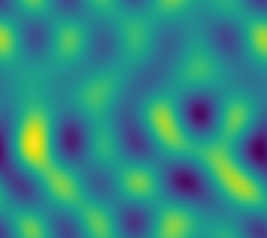
\includegraphics[interpolate=true,width=2.670000in,height=2.380000in]{burgers_forcing_0.1-img0.png}}%
\end{pgfscope}%
\begin{pgfscope}%
\pgfsetbuttcap%
\pgfsetroundjoin%
\definecolor{currentfill}{rgb}{0.000000,0.000000,0.000000}%
\pgfsetfillcolor{currentfill}%
\pgfsetlinewidth{0.803000pt}%
\definecolor{currentstroke}{rgb}{0.000000,0.000000,0.000000}%
\pgfsetstrokecolor{currentstroke}%
\pgfsetdash{}{0pt}%
\pgfsys@defobject{currentmarker}{\pgfqpoint{0.000000in}{-0.048611in}}{\pgfqpoint{0.000000in}{0.000000in}}{%
\pgfpathmoveto{\pgfqpoint{0.000000in}{0.000000in}}%
\pgfpathlineto{\pgfqpoint{0.000000in}{-0.048611in}}%
\pgfusepath{stroke,fill}%
}%
\begin{pgfscope}%
\pgfsys@transformshift{0.567820in}{0.517039in}%
\pgfsys@useobject{currentmarker}{}%
\end{pgfscope}%
\end{pgfscope}%
\begin{pgfscope}%
\definecolor{textcolor}{rgb}{0.000000,0.000000,0.000000}%
\pgfsetstrokecolor{textcolor}%
\pgfsetfillcolor{textcolor}%
\pgftext[x=0.567820in,y=0.419816in,,top]{\color{textcolor}\rmfamily\fontsize{12.000000}{14.400000}\selectfont 0.0}%
\end{pgfscope}%
\begin{pgfscope}%
\pgfsetbuttcap%
\pgfsetroundjoin%
\definecolor{currentfill}{rgb}{0.000000,0.000000,0.000000}%
\pgfsetfillcolor{currentfill}%
\pgfsetlinewidth{0.803000pt}%
\definecolor{currentstroke}{rgb}{0.000000,0.000000,0.000000}%
\pgfsetstrokecolor{currentstroke}%
\pgfsetdash{}{0pt}%
\pgfsys@defobject{currentmarker}{\pgfqpoint{0.000000in}{-0.048611in}}{\pgfqpoint{0.000000in}{0.000000in}}{%
\pgfpathmoveto{\pgfqpoint{0.000000in}{0.000000in}}%
\pgfpathlineto{\pgfqpoint{0.000000in}{-0.048611in}}%
\pgfusepath{stroke,fill}%
}%
\begin{pgfscope}%
\pgfsys@transformshift{1.234291in}{0.517039in}%
\pgfsys@useobject{currentmarker}{}%
\end{pgfscope}%
\end{pgfscope}%
\begin{pgfscope}%
\definecolor{textcolor}{rgb}{0.000000,0.000000,0.000000}%
\pgfsetstrokecolor{textcolor}%
\pgfsetfillcolor{textcolor}%
\pgftext[x=1.234291in,y=0.419816in,,top]{\color{textcolor}\rmfamily\fontsize{12.000000}{14.400000}\selectfont 0.5}%
\end{pgfscope}%
\begin{pgfscope}%
\pgfsetbuttcap%
\pgfsetroundjoin%
\definecolor{currentfill}{rgb}{0.000000,0.000000,0.000000}%
\pgfsetfillcolor{currentfill}%
\pgfsetlinewidth{0.803000pt}%
\definecolor{currentstroke}{rgb}{0.000000,0.000000,0.000000}%
\pgfsetstrokecolor{currentstroke}%
\pgfsetdash{}{0pt}%
\pgfsys@defobject{currentmarker}{\pgfqpoint{0.000000in}{-0.048611in}}{\pgfqpoint{0.000000in}{0.000000in}}{%
\pgfpathmoveto{\pgfqpoint{0.000000in}{0.000000in}}%
\pgfpathlineto{\pgfqpoint{0.000000in}{-0.048611in}}%
\pgfusepath{stroke,fill}%
}%
\begin{pgfscope}%
\pgfsys@transformshift{1.900762in}{0.517039in}%
\pgfsys@useobject{currentmarker}{}%
\end{pgfscope}%
\end{pgfscope}%
\begin{pgfscope}%
\definecolor{textcolor}{rgb}{0.000000,0.000000,0.000000}%
\pgfsetstrokecolor{textcolor}%
\pgfsetfillcolor{textcolor}%
\pgftext[x=1.900762in,y=0.419816in,,top]{\color{textcolor}\rmfamily\fontsize{12.000000}{14.400000}\selectfont 1.0}%
\end{pgfscope}%
\begin{pgfscope}%
\pgfsetbuttcap%
\pgfsetroundjoin%
\definecolor{currentfill}{rgb}{0.000000,0.000000,0.000000}%
\pgfsetfillcolor{currentfill}%
\pgfsetlinewidth{0.803000pt}%
\definecolor{currentstroke}{rgb}{0.000000,0.000000,0.000000}%
\pgfsetstrokecolor{currentstroke}%
\pgfsetdash{}{0pt}%
\pgfsys@defobject{currentmarker}{\pgfqpoint{0.000000in}{-0.048611in}}{\pgfqpoint{0.000000in}{0.000000in}}{%
\pgfpathmoveto{\pgfqpoint{0.000000in}{0.000000in}}%
\pgfpathlineto{\pgfqpoint{0.000000in}{-0.048611in}}%
\pgfusepath{stroke,fill}%
}%
\begin{pgfscope}%
\pgfsys@transformshift{2.567232in}{0.517039in}%
\pgfsys@useobject{currentmarker}{}%
\end{pgfscope}%
\end{pgfscope}%
\begin{pgfscope}%
\definecolor{textcolor}{rgb}{0.000000,0.000000,0.000000}%
\pgfsetstrokecolor{textcolor}%
\pgfsetfillcolor{textcolor}%
\pgftext[x=2.567232in,y=0.419816in,,top]{\color{textcolor}\rmfamily\fontsize{12.000000}{14.400000}\selectfont 1.5}%
\end{pgfscope}%
\begin{pgfscope}%
\pgfsetbuttcap%
\pgfsetroundjoin%
\definecolor{currentfill}{rgb}{0.000000,0.000000,0.000000}%
\pgfsetfillcolor{currentfill}%
\pgfsetlinewidth{0.803000pt}%
\definecolor{currentstroke}{rgb}{0.000000,0.000000,0.000000}%
\pgfsetstrokecolor{currentstroke}%
\pgfsetdash{}{0pt}%
\pgfsys@defobject{currentmarker}{\pgfqpoint{0.000000in}{-0.048611in}}{\pgfqpoint{0.000000in}{0.000000in}}{%
\pgfpathmoveto{\pgfqpoint{0.000000in}{0.000000in}}%
\pgfpathlineto{\pgfqpoint{0.000000in}{-0.048611in}}%
\pgfusepath{stroke,fill}%
}%
\begin{pgfscope}%
\pgfsys@transformshift{3.233703in}{0.517039in}%
\pgfsys@useobject{currentmarker}{}%
\end{pgfscope}%
\end{pgfscope}%
\begin{pgfscope}%
\definecolor{textcolor}{rgb}{0.000000,0.000000,0.000000}%
\pgfsetstrokecolor{textcolor}%
\pgfsetfillcolor{textcolor}%
\pgftext[x=3.233703in,y=0.419816in,,top]{\color{textcolor}\rmfamily\fontsize{12.000000}{14.400000}\selectfont 2.0}%
\end{pgfscope}%
\begin{pgfscope}%
\definecolor{textcolor}{rgb}{0.000000,0.000000,0.000000}%
\pgfsetstrokecolor{textcolor}%
\pgfsetfillcolor{textcolor}%
\pgftext[x=1.900762in,y=0.202965in,,top]{\color{textcolor}\rmfamily\fontsize{12.000000}{14.400000}\selectfont Space}%
\end{pgfscope}%
\begin{pgfscope}%
\pgfsetbuttcap%
\pgfsetroundjoin%
\definecolor{currentfill}{rgb}{0.000000,0.000000,0.000000}%
\pgfsetfillcolor{currentfill}%
\pgfsetlinewidth{0.803000pt}%
\definecolor{currentstroke}{rgb}{0.000000,0.000000,0.000000}%
\pgfsetstrokecolor{currentstroke}%
\pgfsetdash{}{0pt}%
\pgfsys@defobject{currentmarker}{\pgfqpoint{-0.048611in}{0.000000in}}{\pgfqpoint{-0.000000in}{0.000000in}}{%
\pgfpathmoveto{\pgfqpoint{-0.000000in}{0.000000in}}%
\pgfpathlineto{\pgfqpoint{-0.048611in}{0.000000in}}%
\pgfusepath{stroke,fill}%
}%
\begin{pgfscope}%
\pgfsys@transformshift{0.567820in}{0.517039in}%
\pgfsys@useobject{currentmarker}{}%
\end{pgfscope}%
\end{pgfscope}%
\begin{pgfscope}%
\definecolor{textcolor}{rgb}{0.000000,0.000000,0.000000}%
\pgfsetstrokecolor{textcolor}%
\pgfsetfillcolor{textcolor}%
\pgftext[x=0.364559in, y=0.453725in, left, base]{\color{textcolor}\rmfamily\fontsize{12.000000}{14.400000}\selectfont 0}%
\end{pgfscope}%
\begin{pgfscope}%
\pgfsetbuttcap%
\pgfsetroundjoin%
\definecolor{currentfill}{rgb}{0.000000,0.000000,0.000000}%
\pgfsetfillcolor{currentfill}%
\pgfsetlinewidth{0.803000pt}%
\definecolor{currentstroke}{rgb}{0.000000,0.000000,0.000000}%
\pgfsetstrokecolor{currentstroke}%
\pgfsetdash{}{0pt}%
\pgfsys@defobject{currentmarker}{\pgfqpoint{-0.048611in}{0.000000in}}{\pgfqpoint{-0.000000in}{0.000000in}}{%
\pgfpathmoveto{\pgfqpoint{-0.000000in}{0.000000in}}%
\pgfpathlineto{\pgfqpoint{-0.048611in}{0.000000in}}%
\pgfusepath{stroke,fill}%
}%
\begin{pgfscope}%
\pgfsys@transformshift{0.567820in}{0.992634in}%
\pgfsys@useobject{currentmarker}{}%
\end{pgfscope}%
\end{pgfscope}%
\begin{pgfscope}%
\definecolor{textcolor}{rgb}{0.000000,0.000000,0.000000}%
\pgfsetstrokecolor{textcolor}%
\pgfsetfillcolor{textcolor}%
\pgftext[x=0.364559in, y=0.929320in, left, base]{\color{textcolor}\rmfamily\fontsize{12.000000}{14.400000}\selectfont 2}%
\end{pgfscope}%
\begin{pgfscope}%
\pgfsetbuttcap%
\pgfsetroundjoin%
\definecolor{currentfill}{rgb}{0.000000,0.000000,0.000000}%
\pgfsetfillcolor{currentfill}%
\pgfsetlinewidth{0.803000pt}%
\definecolor{currentstroke}{rgb}{0.000000,0.000000,0.000000}%
\pgfsetstrokecolor{currentstroke}%
\pgfsetdash{}{0pt}%
\pgfsys@defobject{currentmarker}{\pgfqpoint{-0.048611in}{0.000000in}}{\pgfqpoint{-0.000000in}{0.000000in}}{%
\pgfpathmoveto{\pgfqpoint{-0.000000in}{0.000000in}}%
\pgfpathlineto{\pgfqpoint{-0.048611in}{0.000000in}}%
\pgfusepath{stroke,fill}%
}%
\begin{pgfscope}%
\pgfsys@transformshift{0.567820in}{1.468230in}%
\pgfsys@useobject{currentmarker}{}%
\end{pgfscope}%
\end{pgfscope}%
\begin{pgfscope}%
\definecolor{textcolor}{rgb}{0.000000,0.000000,0.000000}%
\pgfsetstrokecolor{textcolor}%
\pgfsetfillcolor{textcolor}%
\pgftext[x=0.364559in, y=1.404916in, left, base]{\color{textcolor}\rmfamily\fontsize{12.000000}{14.400000}\selectfont 4}%
\end{pgfscope}%
\begin{pgfscope}%
\pgfsetbuttcap%
\pgfsetroundjoin%
\definecolor{currentfill}{rgb}{0.000000,0.000000,0.000000}%
\pgfsetfillcolor{currentfill}%
\pgfsetlinewidth{0.803000pt}%
\definecolor{currentstroke}{rgb}{0.000000,0.000000,0.000000}%
\pgfsetstrokecolor{currentstroke}%
\pgfsetdash{}{0pt}%
\pgfsys@defobject{currentmarker}{\pgfqpoint{-0.048611in}{0.000000in}}{\pgfqpoint{-0.000000in}{0.000000in}}{%
\pgfpathmoveto{\pgfqpoint{-0.000000in}{0.000000in}}%
\pgfpathlineto{\pgfqpoint{-0.048611in}{0.000000in}}%
\pgfusepath{stroke,fill}%
}%
\begin{pgfscope}%
\pgfsys@transformshift{0.567820in}{1.943825in}%
\pgfsys@useobject{currentmarker}{}%
\end{pgfscope}%
\end{pgfscope}%
\begin{pgfscope}%
\definecolor{textcolor}{rgb}{0.000000,0.000000,0.000000}%
\pgfsetstrokecolor{textcolor}%
\pgfsetfillcolor{textcolor}%
\pgftext[x=0.364559in, y=1.880511in, left, base]{\color{textcolor}\rmfamily\fontsize{12.000000}{14.400000}\selectfont 6}%
\end{pgfscope}%
\begin{pgfscope}%
\pgfsetbuttcap%
\pgfsetroundjoin%
\definecolor{currentfill}{rgb}{0.000000,0.000000,0.000000}%
\pgfsetfillcolor{currentfill}%
\pgfsetlinewidth{0.803000pt}%
\definecolor{currentstroke}{rgb}{0.000000,0.000000,0.000000}%
\pgfsetstrokecolor{currentstroke}%
\pgfsetdash{}{0pt}%
\pgfsys@defobject{currentmarker}{\pgfqpoint{-0.048611in}{0.000000in}}{\pgfqpoint{-0.000000in}{0.000000in}}{%
\pgfpathmoveto{\pgfqpoint{-0.000000in}{0.000000in}}%
\pgfpathlineto{\pgfqpoint{-0.048611in}{0.000000in}}%
\pgfusepath{stroke,fill}%
}%
\begin{pgfscope}%
\pgfsys@transformshift{0.567820in}{2.419421in}%
\pgfsys@useobject{currentmarker}{}%
\end{pgfscope}%
\end{pgfscope}%
\begin{pgfscope}%
\definecolor{textcolor}{rgb}{0.000000,0.000000,0.000000}%
\pgfsetstrokecolor{textcolor}%
\pgfsetfillcolor{textcolor}%
\pgftext[x=0.364559in, y=2.356107in, left, base]{\color{textcolor}\rmfamily\fontsize{12.000000}{14.400000}\selectfont 8}%
\end{pgfscope}%
\begin{pgfscope}%
\pgfsetbuttcap%
\pgfsetroundjoin%
\definecolor{currentfill}{rgb}{0.000000,0.000000,0.000000}%
\pgfsetfillcolor{currentfill}%
\pgfsetlinewidth{0.803000pt}%
\definecolor{currentstroke}{rgb}{0.000000,0.000000,0.000000}%
\pgfsetstrokecolor{currentstroke}%
\pgfsetdash{}{0pt}%
\pgfsys@defobject{currentmarker}{\pgfqpoint{-0.048611in}{0.000000in}}{\pgfqpoint{-0.000000in}{0.000000in}}{%
\pgfpathmoveto{\pgfqpoint{-0.000000in}{0.000000in}}%
\pgfpathlineto{\pgfqpoint{-0.048611in}{0.000000in}}%
\pgfusepath{stroke,fill}%
}%
\begin{pgfscope}%
\pgfsys@transformshift{0.567820in}{2.895016in}%
\pgfsys@useobject{currentmarker}{}%
\end{pgfscope}%
\end{pgfscope}%
\begin{pgfscope}%
\definecolor{textcolor}{rgb}{0.000000,0.000000,0.000000}%
\pgfsetstrokecolor{textcolor}%
\pgfsetfillcolor{textcolor}%
\pgftext[x=0.258521in, y=2.831702in, left, base]{\color{textcolor}\rmfamily\fontsize{12.000000}{14.400000}\selectfont 10}%
\end{pgfscope}%
\begin{pgfscope}%
\definecolor{textcolor}{rgb}{0.000000,0.000000,0.000000}%
\pgfsetstrokecolor{textcolor}%
\pgfsetfillcolor{textcolor}%
\pgftext[x=0.202965in,y=1.706027in,,bottom,rotate=90.000000]{\color{textcolor}\rmfamily\fontsize{12.000000}{14.400000}\selectfont Time}%
\end{pgfscope}%
\begin{pgfscope}%
\pgfsetrectcap%
\pgfsetmiterjoin%
\pgfsetlinewidth{0.803000pt}%
\definecolor{currentstroke}{rgb}{0.000000,0.000000,0.000000}%
\pgfsetstrokecolor{currentstroke}%
\pgfsetdash{}{0pt}%
\pgfpathmoveto{\pgfqpoint{0.567820in}{0.517039in}}%
\pgfpathlineto{\pgfqpoint{0.567820in}{2.895016in}}%
\pgfusepath{stroke}%
\end{pgfscope}%
\begin{pgfscope}%
\pgfsetrectcap%
\pgfsetmiterjoin%
\pgfsetlinewidth{0.803000pt}%
\definecolor{currentstroke}{rgb}{0.000000,0.000000,0.000000}%
\pgfsetstrokecolor{currentstroke}%
\pgfsetdash{}{0pt}%
\pgfpathmoveto{\pgfqpoint{3.233703in}{0.517039in}}%
\pgfpathlineto{\pgfqpoint{3.233703in}{2.895016in}}%
\pgfusepath{stroke}%
\end{pgfscope}%
\begin{pgfscope}%
\pgfsetrectcap%
\pgfsetmiterjoin%
\pgfsetlinewidth{0.803000pt}%
\definecolor{currentstroke}{rgb}{0.000000,0.000000,0.000000}%
\pgfsetstrokecolor{currentstroke}%
\pgfsetdash{}{0pt}%
\pgfpathmoveto{\pgfqpoint{0.567820in}{0.517039in}}%
\pgfpathlineto{\pgfqpoint{3.233703in}{0.517039in}}%
\pgfusepath{stroke}%
\end{pgfscope}%
\begin{pgfscope}%
\pgfsetrectcap%
\pgfsetmiterjoin%
\pgfsetlinewidth{0.803000pt}%
\definecolor{currentstroke}{rgb}{0.000000,0.000000,0.000000}%
\pgfsetstrokecolor{currentstroke}%
\pgfsetdash{}{0pt}%
\pgfpathmoveto{\pgfqpoint{0.567820in}{2.895016in}}%
\pgfpathlineto{\pgfqpoint{3.233703in}{2.895016in}}%
\pgfusepath{stroke}%
\end{pgfscope}%
\begin{pgfscope}%
\pgfsetbuttcap%
\pgfsetmiterjoin%
\pgfsetlinewidth{0.000000pt}%
\definecolor{currentstroke}{rgb}{0.000000,0.000000,0.000000}%
\pgfsetstrokecolor{currentstroke}%
\pgfsetstrokeopacity{0.000000}%
\pgfsetdash{}{0pt}%
\pgfpathmoveto{\pgfqpoint{3.499525in}{0.517039in}}%
\pgfpathlineto{\pgfqpoint{3.618424in}{0.517039in}}%
\pgfpathlineto{\pgfqpoint{3.618424in}{2.895016in}}%
\pgfpathlineto{\pgfqpoint{3.499525in}{2.895016in}}%
\pgfpathlineto{\pgfqpoint{3.499525in}{0.517039in}}%
\pgfpathclose%
\pgfusepath{}%
\end{pgfscope}%
\begin{pgfscope}%
\pgfsys@transformshift{3.500000in}{0.520000in}%
\pgftext[left,bottom]{
\includegraphics[interpolate=true,width=0.120000in,height=2.380000in]{burgers_forcing_0.1-img1.png}}%
\end{pgfscope}%
\begin{pgfscope}%
\pgfsetbuttcap%
\pgfsetroundjoin%
\definecolor{currentfill}{rgb}{0.000000,0.000000,0.000000}%
\pgfsetfillcolor{currentfill}%
\pgfsetlinewidth{0.803000pt}%
\definecolor{currentstroke}{rgb}{0.000000,0.000000,0.000000}%
\pgfsetstrokecolor{currentstroke}%
\pgfsetdash{}{0pt}%
\pgfsys@defobject{currentmarker}{\pgfqpoint{0.000000in}{0.000000in}}{\pgfqpoint{0.048611in}{0.000000in}}{%
\pgfpathmoveto{\pgfqpoint{0.000000in}{0.000000in}}%
\pgfpathlineto{\pgfqpoint{0.048611in}{0.000000in}}%
\pgfusepath{stroke,fill}%
}%
\begin{pgfscope}%
\pgfsys@transformshift{3.618424in}{1.051832in}%
\pgfsys@useobject{currentmarker}{}%
\end{pgfscope}%
\end{pgfscope}%
\begin{pgfscope}%
\definecolor{textcolor}{rgb}{0.000000,0.000000,0.000000}%
\pgfsetstrokecolor{textcolor}%
\pgfsetfillcolor{textcolor}%
\pgftext[x=3.715646in, y=0.988519in, left, base]{\color{textcolor}\rmfamily\fontsize{12.000000}{14.400000}\selectfont \ensuremath{-}2}%
\end{pgfscope}%
\begin{pgfscope}%
\pgfsetbuttcap%
\pgfsetroundjoin%
\definecolor{currentfill}{rgb}{0.000000,0.000000,0.000000}%
\pgfsetfillcolor{currentfill}%
\pgfsetlinewidth{0.803000pt}%
\definecolor{currentstroke}{rgb}{0.000000,0.000000,0.000000}%
\pgfsetstrokecolor{currentstroke}%
\pgfsetdash{}{0pt}%
\pgfsys@defobject{currentmarker}{\pgfqpoint{0.000000in}{0.000000in}}{\pgfqpoint{0.048611in}{0.000000in}}{%
\pgfpathmoveto{\pgfqpoint{0.000000in}{0.000000in}}%
\pgfpathlineto{\pgfqpoint{0.048611in}{0.000000in}}%
\pgfusepath{stroke,fill}%
}%
\begin{pgfscope}%
\pgfsys@transformshift{3.618424in}{1.679688in}%
\pgfsys@useobject{currentmarker}{}%
\end{pgfscope}%
\end{pgfscope}%
\begin{pgfscope}%
\definecolor{textcolor}{rgb}{0.000000,0.000000,0.000000}%
\pgfsetstrokecolor{textcolor}%
\pgfsetfillcolor{textcolor}%
\pgftext[x=3.715646in, y=1.616374in, left, base]{\color{textcolor}\rmfamily\fontsize{12.000000}{14.400000}\selectfont 0}%
\end{pgfscope}%
\begin{pgfscope}%
\pgfsetbuttcap%
\pgfsetroundjoin%
\definecolor{currentfill}{rgb}{0.000000,0.000000,0.000000}%
\pgfsetfillcolor{currentfill}%
\pgfsetlinewidth{0.803000pt}%
\definecolor{currentstroke}{rgb}{0.000000,0.000000,0.000000}%
\pgfsetstrokecolor{currentstroke}%
\pgfsetdash{}{0pt}%
\pgfsys@defobject{currentmarker}{\pgfqpoint{0.000000in}{0.000000in}}{\pgfqpoint{0.048611in}{0.000000in}}{%
\pgfpathmoveto{\pgfqpoint{0.000000in}{0.000000in}}%
\pgfpathlineto{\pgfqpoint{0.048611in}{0.000000in}}%
\pgfusepath{stroke,fill}%
}%
\begin{pgfscope}%
\pgfsys@transformshift{3.618424in}{2.307543in}%
\pgfsys@useobject{currentmarker}{}%
\end{pgfscope}%
\end{pgfscope}%
\begin{pgfscope}%
\definecolor{textcolor}{rgb}{0.000000,0.000000,0.000000}%
\pgfsetstrokecolor{textcolor}%
\pgfsetfillcolor{textcolor}%
\pgftext[x=3.715646in, y=2.244229in, left, base]{\color{textcolor}\rmfamily\fontsize{12.000000}{14.400000}\selectfont 2}%
\end{pgfscope}%
\begin{pgfscope}%
\pgfsetrectcap%
\pgfsetmiterjoin%
\pgfsetlinewidth{0.803000pt}%
\definecolor{currentstroke}{rgb}{0.000000,0.000000,0.000000}%
\pgfsetstrokecolor{currentstroke}%
\pgfsetdash{}{0pt}%
\pgfpathmoveto{\pgfqpoint{3.499525in}{0.517039in}}%
\pgfpathlineto{\pgfqpoint{3.558975in}{0.517039in}}%
\pgfpathlineto{\pgfqpoint{3.618424in}{0.517039in}}%
\pgfpathlineto{\pgfqpoint{3.618424in}{2.895016in}}%
\pgfpathlineto{\pgfqpoint{3.558975in}{2.895016in}}%
\pgfpathlineto{\pgfqpoint{3.499525in}{2.895016in}}%
\pgfpathlineto{\pgfqpoint{3.499525in}{0.517039in}}%
\pgfpathclose%
\pgfusepath{stroke}%
\end{pgfscope}%
\end{pgfpicture}%
\makeatother%
\endgroup%

    \end{adjustbox}
    \caption{Forcing function for \(\nu=0.1\).}\label{fig:burgers_forcing_0.1}
  \end{subfigure}
  \caption{Example sample pairs of solution and forcing terms for the Burgers' equation dataset.}\label{fig:burgers_data}
\end{figure}

\section{Data Retrieval}\label{sec:data_retrieval}
\noindent The second data acquisition approach retrieves data of a from an external source. This approach downloads the external data to a local machine. In this study, the specific dataset that will be used is the ERA5 dataset from the European Center for Medium-range Weather Forecast (ECMWF). Specifically, the ERA5 dataset is a reanalysis which means it combines observational data from all over the world in order to present a more complete picture of the weather system. This combination process, named 4D variational data assimilation, takes into account the physics known to be involved in the system. As an example weather station data which take measurements such as wind speed, humidity, and temperature of the immediate surroundings of the weather station is very limited in giving a broader picture of weather over a larger area. Even technologies like earth observations satellites are limited to what they can observe at any single point in time as most cannot see the entirety of the earth's surface at once. The ERA5 dataset specifically, assimilates previous forecasts with observational data every 12 hours. The ERA5 reanalysis is available at the following URL (\url{https://cds.climate.copernicus.eu/datasets/reanalysis-era5-single-levels}).

The original dataset made available by ECMWF has a grid size of \ang{0.25} by \ang{0.25} in latitude and longitude for atmospheric data. Data of oceanic waves are also available at a coarser grid size of \ang{0.5} by \ang{0.5}. However, we will use a cloud optimized version called WeatherBench2 that is easier to retrieve \autocite{raspWeatherBench2Benchmark2023}. This is because the data is available in several more grid sizes such as \ang{1.5}. In addition, the data can be readily downloaded to a local machine without waiting for further processing on the server. The guide for working with the dataset is available at (\url{https://weatherbench2.readthedocs.io/en/latest/data-guide.html}). In our specific case, we use the version labeled \verb|1959-2023_01_10-6h-64x32_equiangular_conservative.zarr|. This dataset spans from year 1959 to 2023 with a grid size of \ang{5.625} or resolution of 64 by 32 which spans from \ang{-87.19} to \ang{87.19} in latitude and \ang{0.0} to \ang{354.4} in longitude. The dataset is also resampled down to 6-hour intervals that starts at midnight UTC January 1959 1\textsuperscript{st} and ends at 18:00 UTC January 10\textsuperscript{th} 2023.

While the original data provided by ECMWF is available in NetCDF or GRIB, the WeatherBench2 version is provided using the Zarr format in a Google Cloud Storage Bucket. This setup allows the use of libraries that support the Zarr format to access the dataset remotely. The particular library we use is called \emph{Xarray} version \verb|2024.9.0| \autocite{hoyer2017xarray,hoyerXarray2024}. Accessing the remote dataset is done as shown in \lccref{fig:access_remote_zarr}. In order to ensure access is granted, the storage option token is set to anon so that the method uses the anonymous only public access mode of authentication \autocite{GCSFSGCSFs2023122post1+1g8e500c6dirty}.

\begin{figure}[H]
  \centering
  \begin{lstlisting}[language=Python]
  import xarray as xr
  xr.open_zarr(
      "DATASET_ADDRESS",
      storage_options = {"token": "anon"},
  )
  \end{lstlisting}
  \caption{Example of using Xarray to access a publicly accessible Zarr dataset hosted on Google Cloud Storage Bucket.}\label{fig:access_remote_zarr}
\end{figure}

The dataset includes 62 variables with some variables also spanning 13 discrete vertical levels in the atmosphere. For our use, we will only be using the 2-meter temperature of the atmosphere. This is the air temperature 2 meters above the surface be it land, sea, or inland water. This variable is in units of kelvin. The values of this variable is obtained by interpolating between the model values at the surface and the lowest model vertical level. We also limit the time range to ... An example of the data that was retrieved can be seen in .
% TODO: talk about selecting the time here
% ECMWF description
% - Role
% - legitimacy
% - Weatherbench2
% data description
% - data assimilation, maybe reference a general description
% - variables
% - dimensions/coordinates (time, spatial) and resolution in each
% - climatology

\section{Design of Computational Model}\label{sec:computational_model_design}
\noindent In this section, we will discuss the design of the computational model that is proposed in this work. An illustration of the computational model is show in \lccref{fig:computational_model}.

\begin{figure}[H]
  \centering
  \begin{adjustbox}{max width=\textwidth}
    \tikzfig{figures/computational_model}
  \end{adjustbox}
  \caption{Computational Model of SpectralSVR.}\label{fig:computational_model}
\end{figure}

The computational model is divided into four large phases. The processes within these phases are based on the broad outcomes of the phase. The phases themselves are data preparation, data transformation, model training, and model evaluation. Each phase is composed of processes that together works toward the output of the larger process. At the end, a final process of analysis and interpretation is carried out.

\subsection{Data Preparation}
\noindent The data preparation phase starts off the computation by preparing the data that is to be used in this study. This phase starts with specifying the problem to be solved. This translates to the dataset that will be used to represent these problems. The first type of dataset is generated based on a known governing equation or PDE\@. Using said equation, the goal is to generate pairs of functions that are related to each other by the equation. In the next process, generally, the solution function is first generated randomly. This is done by generating random numbers to use as coefficients of a set of basis functions. Then parameters of the equation is determined, such as term coefficients. Using the generated solution and predetermined parameters, a forcing term can generally be computed to satisfy the equation. Augmentations such as noise can then be added in the final process which is evaluating the function values. These processes result in a generated dataset. To verify the generation method and any models trained on the generated data one can use exact analytical solutions of the governing equations.

The second type of dataset is retrieved from an external source. The data source is first identified, in our case it is the WeatherBench 2 collection of datasets. The specific dataset from the collection of different dataset versions is first determined. The dataset is available in the \emph{Zarr} format. And then, we determine the filters for the portions of the dataset we are interested in. Once the dataset and filters are determined, the retrieval process starts by accessing the dataset using the \emph{Xarray} library \autocite{hoyer2017xarray,hoyerXarray2024}. The filters are applied as in .... % TODO: add figure for code of the filtering process and local save process
Finally, the filtered version is stored locally. The local dataset is also stored in the \emph{Zarr} format.

\subsection{Data Transformation}\label{sec:data_transformation}
\noindent The second phase of the computational model transforms the data that has been prepared into a form that can be used with the proposed model. In this study, there are two ways a dataset can be used. The first and simplest way is to predict the solution function from the forcing term for a given set of PDE parameters. In this case, the input function is the forcing term. In other words, the input function is the predictor or independent variable that will be used to predict the solution function. As such, the output function is the solution function. The antiderivative dataset is used in this way. The derivative, which represents the acceleration function, is used to predict the velocity function. Which means that the input function is the acceleration function and the output function is the velocity function.

The second use of a dataset depends on whether it can be interpreted as a mapping of a previous function to the next function. In other words, a series of functions related to the previous function as a sum of the previous function and a perturbation. A commonly used form of this are time series. Generally, a time series can be represented as \lccref{eq:time_step_function}. This function describes the evolution of function \(f\) as a sum of some initial state \(f^0\) and perturbation which is its rate of change \(\dv{f}{t}\) at a point in time close to the current time multiplied by the time step \(\delta t\). This is the first order Taylor polynomial. Adding more terms with higher order derivatives can be done to increase the accuracy. This describes the same process that is used in the finite difference method.
\begin{equation}
  f^{t+1} = f^{t} + \delta t \times \dv{f}{t} + \dots \label{eq:time_step_function}
\end{equation}
In this case the previous function and any other independent variables like the forcing term involved in the right-hand side of the equation is used to predict the difference between the future state and the current state. It would mean that each sample function in the data would need to at least have two dimensions. This is because one dimension represents the evolution of the function over time, while the other dimensions define the spatial domain where the function's values are computed at each time step. This condition is true for both the Burgers' equation dataset and the WeatherBench 2 collection of ERA5 datasets. First, the Burgers' equation dataset, while is also able to be used in the first way as a mapping between the forcing term and the solution, one of the traditional ways of solving it is using the method of lines. This entails solving the dimensions other that time with methods such as the finite differences method or the spectral method. The time dimension is then separately solved using the finite differences method such as the form shown in \lccref{eq:time_step_function} \autocite{schiesserNumericalMethodLines2012,sadikuSimpleIntroductionMethod2000}. This is the form that the Burgers' equation dataset will be used in. In this case, algebraic manipulation of \lccref{eq:forced_viscous_burgers} results in the time derivative of the solution as in \lccref{eq:forced_viscous_burgers_time_derivative}.
\begin{align}
  \pdv{u}{t} = f - u\pdv{u}{x} + \nu\pdv[2]{u}{x} \label{eq:forced_viscous_burgers_time_derivative}
\end{align}
The most important component of the right-hand side of the equation, the time derivative, is expressed in terms of the solution function, the forcing term and any other partial derivatives. Because of this, it means we can train the model to learn the relationship between the solution function combined with the forcing term and the time derivative. Putting this together with \lccref{eq:time_step_function}, it is possible to predict the solution function in a future time based on the current solution function and forcing term. The input functions in this case are both the value of the solution function and the forcing term at the current time step. The output function is the time derivative which is computed by rearranging \lccref{eq:time_step_function} resulting in \lccref{eq:time_derivative_time_step_function}.
\begin{equation}
  \dv{f}{t} = \frac{f^{t+1} - f^{t}}{\delta t} \label{eq:time_derivative_time_step_function}
\end{equation}
Perhaps in a more obvious manner, the same is also applied to the WeatherBench 2 collection of ERA5 datasets. The 2-meter temperature is a series of snapshots in time of the distribution of temperature all over the world at 2 meters above the surface. The input function in this case is the temperature distribution at the current time step. The output function is the time derivative of the temperature distribution computed using \lccref{eq:time_derivative_time_step_function}.

The input and output functions are then transformed into basis coefficients using the Fourier transform. % TODO: add reference to fourier transform in chapter 2
Once the coefficients are computed, the input and output sample pairs are split into train, test, and validation subsets. For the first type of input and output function pair, since the samples are independent of each other, a random sampling of the dataset without replacement is done to select the samples for each subset. For the second type of input and output function pairs, if there are multiple samples of functions as in the Burgers' equation dataset, the same process with random sampling is followed. On the other hand, if only one function sample is available, such as the WeatherBench 2 dataset, an issue that arises is the fact that the samples are dependent on one another. This is because a previous time step influences the next time step. This is a problem for generalizing the learned model, since random sampling would lead to the model learning information in the future of the testing subset \autocite{kapoorLeakageReproducibilityCrisis2023,kaufmanLeakageDataMining2012}. As such, the portioning of the dataset is done by dividing the sample into different sections of the function in time.

Finally, the data is scaled. This is done because of how support vector machines require scaling for inputs in order to perform well with certain hyperparameters such as the RBF kernel \autocite{ben-hurUsersGuideSupport2010}. For our case we use standard scaling based on the inputs of the training subset. This approach transforms the dataset by manipulating the distribution characteristics of the dataset \autocite{ahsanEffectDataScaling2021}. Specifically, the standard deviation \(\sigma \) and mean \(x_0\) of the dataset values \(x\) are processed such that the resulting values have a mean of 0 and standard deviation of 1. The function shown in \lccref{eq:standard_scaler} represents how each sample is processed with respect to the standard deviation \(\sigma \) and mean \(x_0\) of each feature.
\begin{equation}
  z(x;\sigma,x_0)=\frac{x-x_0}{\sigma} \label{eq:standard_scaler}
\end{equation}
The scaling is important for the RBF kernel specifically due to the fact that the kernel utilize a scale parameter. This parameter affects how scale of values influence the kernel. Another and perhaps more general benefit of scaling is the uniformity it enforces across features. This is useful because all feature weigh the outcome equally. In our use case, this equality is a reflection of what the data actually represents. Each feature which is a discretized value or its coefficient representation has equal value to any other feature. No point or coefficient is any more or less value compared to another point or coefficient.

The scaling is applied to input functions only because scaling of the outputs does not affect the performance of the model \autocite{ben-hurUsersGuideSupport2010}. To also prevent information leakage across training and testing sets, the mean and standard deviation of each feature is computed using the training subset only. Once the parameter values are obtained, all input function samples in the dataset are transformed into their scaled versions. This means that the distribution for the testing and validation sets may be outside the target standard deviation and mean. % TODO: add graphs and tables of the resulting preprocessed data

\subsection{Model Training}
\noindent Once the data has been preprocessed, the model is trained using pairs of training features and labels. The training phase is separated into four processes. First, the preprocessed input and output function representation need to be real numbers. This is because the LSSVR model was made to work with real numbers. Any complex values such as Fourier coefficients are represented as flattened pairs of the real and imaginary components of complex values. % TODO: add figure of flattened complex values

The training can proceed to solve \lccref{eq:lssvr_solution}. As the original LSSVR equation was made for regression of a single value of \(\vb{y} \), we constructed an extended the original equation in order to train multiple regression models to predict each coefficient in an output function sample. The assumption of this extension is that the inputs and model hyperparameters such as kernels and the regularization constant \(C \) are the same across individual regressors. Therefore, it follows that the solution vector and target vector can both be transformed into their matrix form with each column representing the individual regressor which results in \lccref{eq:lssvr_solution_vectorized}. This vectorized version is equal to \(m \) separate instances of \lccref{eq:lssvr_solution}. In essence, instead of a vector of scalar sample output values and a vector of model parameters, the extended equation consists of a matrix of rows of vector output values and a matrix of model parameters with each column representing the separate model for each output and row representing the Lagrange multipliers for each sample. The procedure to solve \lccref{eq:lssvr_solution_vectorized} adjusts \lccref{alg:lssvr_training} for the extra dimension spanning the multiple outputs of size \(m\).
\begin{equation} \label{eq:lssvr_solution_vectorized}
  \begin{bmatrix}
    0          & \vb{1}_{n}^{\intercal} \\
    \vb{1}_{n} & \Omega + \frac{I}{C}
  \end{bmatrix}
  \begin{bmatrix}
    b_0           & \cdots & b_m           \\
    \vb{\alpha}_0 & \cdots & \vb{\alpha}_m \\
  \end{bmatrix}
  =
  \begin{bmatrix}
    0        & \cdots & 0        \\
    \vb{y}_0 & \cdots & \vb{y}_m \\
  \end{bmatrix}
\end{equation}

Second, as the training process of an LSSVR described in requires constructing the first matrix on the left-hand side and the matrix on the right-hand side, each component of the matrices themselves will also need to be constructed. The kernel matrix \(\Omega \) is first constructed by computing the kernel values between each sample input with every other sample input. If the training set has \(n \) samples, then the resulting kernel matrix would be of size \(n \) by \(n \).
% Assemble lssvr optimality equation matrices
Third, using the inputs \(\vb{X}\), outputs \(\vb{y}\), predetermined regularization constant \(C \), and the obtained kernel matrix \(\Omega \), \lccref{eq:lssvr_solution_vectorized} is assembled. Finally, the matrix of learned parameters \(\vb{\alpha}\) and \(\vb{b}\), which are the Lagrange multipliers and bias respectively, are solved for using a linear equation solver such as a matrix Moore-Penrose inverse or linear least squares solver.

% TODO: decide if hyperparameter selection is needed and explain why or why not. Maybe hyperparameter selection is done in a phase after the model evaluation with a decision between repeating model training with different hyperparameters or keeping the trained model.
Next, the selection of hyperparameters is done to optimize the model further. As previously mentioned, the hyperparameters are the regularization constant \(C \) and kernel functions including the kernel function parameters.

\subsection{Model Evaluation}
\noindent The fourth phase of the computational model is the evaluation of the learned model. This phase starts with formatting the inputs. If the inputs aren't scaled yet, then it is scaled using the scaling function fitted on the training set. This is the case for new data such as new measurements or an analytical solution of the learned PDE\@. Once the inputs that is to be evaluated is scaled in the same way as the training inputs, the model can predict the corresponding outputs.

The procedure to compute the predicted outputs follows \lccref{alg:lssvr_prediction}. This leads to the second process which is computing the kernel matrix between the training input features \(\vb{X}\) and the evaluation input features \(\vb{U}\). The matrix is constructed as the kernel value between each evaluation sample feature and every training sample feature. For \(p \) evaluation samples and \(n \) training samples, this results in a kernel matrix \(\Omega \) with a shape of \(p \) rows and \(n \) columns.

In the third process, the constructed kernel matrix is then multiplied with the matrix of learned Lagrange multipliers \(\vb{\alpha}\). The multiplication is the matrix multiplication process. Then, the bias vector is added to each row to produce the final predicted outputs \(\vb{v}\). This process is represented by \lccref{eq:lssvr_prediction_vectorized}.
\begin{equation}
  \vb{v} = \Omega\vb{\alpha}+\vb{1}\vb{b} \label{eq:lssvr_prediction_vectorized}
\end{equation}

The fourth process is concerned with the fact that the predicted output \(\vb{v}\) is a matrix of real numbers. The LSSVR output needs to be formatted before it can be used in the proposed model. This is done by converting the outputs into the same format as the training labels. As we use the Fourier basis, the model output is converted back into a matrix of complex numbers using the inverse of the first process during training. Finally, these predicted Fourier basis coefficients can be used to evaluate the predicted functions themselves.

\section{Implementation of Computational Model}
\noindent This section discusses the implementation of modeling and approximation of PDEs using LSSVR\@. Using the computational model design in \lccref{sec:computational_model_design}, the computational model is implemented as a library using the Python programming language. The development process itself is based on the iterative development model as mentioned in \lccref{sec:development method}. In this section, the output iterative processes are consolidated and explained together.

\subsection{Analysis}
\noindent The aim of any program that is developed in this study is to model the relationship between functions defined by a partial differential equation or other operators and governing equations. Since the potential subject of modeling can be wide-ranging, the software product that will be developed is a library. This is done so that the tools and proposed model that is developed will be able to be used with a variety of PDEs. With this in mind, the software must also be performant and compatible with the larger machine learning and scientific computing community.

To demonstrate the use and capability of the software, three case studies are chosen to represent the variety of PDEs. The first case study is the antiderivative equation. This simple case is chosen as a proof of concept to show that the proposed model works in the most simple case. The second case study, which is the Burgers' equation, adds a level of complexity because of the nonlinearity involved with the solution function. The third case study, which is the ERA5 weather dataset, was chosen to show how the model performs on data with real world observations incorporated into it. This dataset also presents a challenge because of the uncertainties involved with weather simulation \autocite{herreraReviewCurrentFuture2017}. These datasets are discussed in \lccrefs{sec:data_generation,sec:data_retrieval}.

In addition, the software product is developed within certain limitations. The limitations are:
\begin{enumerate}
  \item The operating and implementation language of the library is Python.
  \item The library is to be used in user code
  \item The library depends on other libraries including the following core dependencies PyTorch, NumPy, Xarray, Zarr, Pandas, and tqdm.
\end{enumerate}

\subsection{Design}\label{sec:implementation_design}
\noindent In this subsection, the architectural design of the software product is explained. The architecture consists of modules with similar concerns. This was chosen because of the intuition built by the use of other libraries with a similar architecture. The broad aim of modeling PDEs with LSSVR and basis functions coefficients can be separated into smaller concerns of data, model, and basis functions. Each of these concerns are addressed by a corresponding module. The explanation of each module are as follows:
\begin{enumerate}
  \item Utilities

        \noindent This module provides basic tools that are used across the entire library. The utilities this module needs to provide include scaling, conversion between real and complex representations of matrices, resizing coefficient tensors, and adaptors for or the traditional ordinary differential equation solvers. Scaling functionality is used for inputs into the support vector machines. And as previously mentioned, since LSSVR only works with real numbers, the tools for converting between complex and their real number representations is also necessary. Another useful tool for working with basis coefficients is a way to resize the coefficients in terms of how many basis functions is desired. An example of the usage is downsizing Fourier coefficients from 12 to 8 modes. The last utility mentioned here provides the ability to solve ordinary differential equations. This utility is useful for generating data for certain types of PDEs such as the Burgers' equation.

  \item Basis Functions

        \noindent As the proposed model will learn the relationships defined by PDEs within the spectral domain, a large proportion of the computation will also concern the use of the basis functions themselves. The module will define the functionality and data structure that is expected to be used when working with basis functions in this library. First and foremost, the central function of this module is to store and facilitate the connection between the coefficients in the spectral domain and their values in the physical domain. This is dependent on the basis functions used. For the Fourier basis that we use in this study, this means that the transformations are the discrete Fourier transform and the discrete inverse Fourier transform. Other than this core functionality, information on the characteristics of the coefficients such as the number of modes, in other words basis functions, should also be provided by this module. In addition, other functionality included in this module are visualization of coefficients in physical space, generation of random functions, time dependent \& complex/real coefficients, noise perturbation of functions, and differential operators.

  \item Model

        \noindent The proposed SpectralSVR model is implemented in this module. As the proposed model essentially wraps a support vector regression model in such a way that it can process coefficients, this module will house the SpectralSVR wrapper itself and the LSSVR variant of support vector regression that is used in this study. The SpectralSVR wrapper must provide three core pieces of functionality. First, it must translate complex input and output samples into their real representations. This applies to both training and evaluation. Second, in addition to predicting the coefficients during evaluation, the wrapper should also be able to predict the function values themselves for any given set of point coordinates. This is important for quick evaluations of a predicted function at an arbitrary point. The third functionality is inverse input function search for a given output. This is useful for inverse problems where the parameters are unknown, but the solution is partially known. Aside from the core functionality, a complementary functionality is testing for the learned model.

        The model module also implements the LSSVR model. This implementation provides two main functionalities. The first is training the LSSVR model with some given model hyperparameters such as the regularization constant and kernel. The second functionality is the evaluation of the learned model. Both functionalities allow for multiple output regression. This is required to learn the mappings for many coefficients at once. Other functionality provided by the implementation include interpretability functions and model serialization for saving and loading the learned model to disk.

  \item Problems

        \noindent This module provides the functionality concerned with generating data. Two out of the three datasets in this study are generated with this module. In general this module provides two pieces of functionality. The first is generation of the data itself. This functionality generates at least two sets of functions that are related to each other by the chosen PDE\@. The generation is based on at least two parameters which are the number of samples to generate and the number of modes or basis functions to generate the coefficients for. The second functionality provided by this module is the residual based on the chosen PDE\@. This is useful to verify if any set of functions comply with the PDE\@. For example, the residual may be used to verify the generated data. Another use is to grade the predictions by the learned model.

\end{enumerate}

The design presented here is the product of multiple iterations that started with building the core model and then the basis functions and finally the data. Throughout the iterations, the utilities were also added to alleviate the need for general tools.

\subsection{Implementation}

\noindent The design in \lccref{sec:implementation_design} is implemented within the same iterative loop. As such, the feedback from tests is immediate, and any fixes can be implemented quickly. The implementation is done using the Python language and a number of Python libraries. To facilitate the management of dependencies, the implementation makes use of the package management tool Poetry \autocite{eustacePoetryPythonPackaging2024}. In addition, the Python version is managed using the tool PyEnv. The implementation process starts with installation of the required dependencies. The dependencies are specified in the \verb|pyproject.toml| as shown in \lccref{fig:poetry_add_deps}.

\begin{figure}[H]
  \centering
  \begin{lstlisting}[language=Toml]
...
[tool.poetry.dependencies]
python = "^3.10.6"
numpy = "^1.24.0"
tqdm = "^4.65.0"
jaxtyping = "^0.2.20"
pandas = "^2.2.2"
torchmetrics = "^1.4.2"
scikit-learn = "^1.5.0"
matplotlib = "^3.9.0"
torch = {version = "^2.4.1+cu124", source = "pytorch-gpu"}
torchvision = {version = "^0.19.1+cu124", source = "pytorch-gpu"}
torchaudio = {version = "^2.4.1+cu124", source = "pytorch-gpu"}
ray = {extras = ["tune"], version = "^2.37.0"}
hyperopt = "^0.2.7"
ipywidgets = "^8.1.5"
torchdiffeq = "^0.2.4"
xarray = "^2024.10.0"
zarr = "^2.18.3"
gcsfs = "^2024.10.0"

[[tool.poetry.source]]
name = "pytorch-gpu"
url = "https://download.pytorch.org/whl/cu124"
priority = "explicit"

[build-system]
requires = ["poetry-core"]
build-backend = "poetry.core.masonry.api"
  \end{lstlisting}
  \caption{Contents of pyproject.toml configuration file that define the dependencies using Poetry.}\label{fig:poetry_add_deps}
\end{figure}

After ensuring that the correct version of python is being used with pyenv, the dependencies specified in the \verb|pyproject.toml| file can be installed using the shell command \verb|poetry install|. At the end of each iteration, the dependencies are subject to change depending on whether any new ones are needed or old dependencies can be removed.

In the following, we will discuss the implementation of each module and how the phases of computational model relates to each implemented functionality. The base data structure that is used in the implementation is the PyTorch Tensor \autocite{Ansel_PyTorch_2_Faster_2024}. Tensors are a generalization of scalars and array-like structures such as vectors and matrices. This is essential since many computations that is done in the proposed model are based on matrices and higher dimensional arrays. PyTorch Tensors allow the elements to be of different data types such as floating point numbers of different precision or even complex numbers. In addition to basic operations for working with the Tensors such as matrix multiplications, PyTorch also provides many algorithms for use when working with Tensors such as linear equation solvers or the Fast Fourier Transform. Another reason for choosing to use PyTorch is the ability to parallelize computation using specialized processors such as GPUs. Lastly, PyTorch is widely used in the machine learning community which reflects on its reliability, wealth of community knowledge and support, and active development.

\subsubsection{Utilities}

\noindent The utilities module provide common tools that are used when working with the developed software. First, because the basis function used in this study is the Fourier basis, a large proportion of concern is the storage of Fourier basis coefficients. The Fourier series representation that is used in this study is the complex representation as show in \lccref{eq:fourier_series}. However, as previously mentioned, least squares support vector machines is constructed to work with real numbers. In order for LSSVR to learn the relationship between complex numbers, a representation of complex numbers in terms of real numbers is necessary. Since sample features and labels for LSSVR need to be flattened into one dimension which result in a matrix with rows of samples, the representation of complex numbers using real numbers can be done after features and labels have been flattened. An example of such a matrix of two samples with four features each can be seen in \lccref{eq:complex_matrix}. To represent the complex number features as real numbers, once can simply split a single complex number into two real numbers. When this is done to the entire matrix of complex numbers, the result is \lccref{eq:complex_matrix_real_rep}.
\begin{align}
  \begin{bmatrix}
    -1.03+0i & -0.52+0.39i & -0.54+0i & -0.52-0.39i \\
    -0.85+0i & -0.39+0.19i & 0.87+0i  & -0.39-0.19i
  \end{bmatrix}\label{eq:complex_matrix} \\
  \begin{bmatrix}
    -1.03 & 0 & -0.52 & 0.39 & -0.54 & 0 & -0.52 & -0.39 \\
    -0.85 & 0 & -0.39 & 0.19 & 0.87  & 0 & -0.39 & -0.19
  \end{bmatrix}\label{eq:complex_matrix_real_rep}
\end{align}
There are several ways to do this in PyTorch, such as extracting the real and imaginary element components into separate matrices and then interleaving the columns to create the real representation. However, a more performant version can be made by using built-in functions of the library that directly allows views of complex valued tensors as real tensors and vice versa. The \verb|view_as_real| and \verb|view_as_complex| functions allow the conversion between real and complex representations by representing complex valued tensors by adding a dimension of size two for each component of complex numbers. The resulting implementation can be seen in \lccref{fig:complex_matrix_conversion_implementation}.
\begin{figure}[H]
  \centering
  \begin{lstlisting}[language=Python]
def to_real_coeff(x: torch.Tensor) -> torch.Tensor:
    return torch.view_as_real(x).flatten(-2)

def to_complex_coeff(x: torch.Tensor) -> torch.Tensor:
  return torch.view_as_complex(
    x.reshape((*x.shape[:-1], -1, 2))
  )
  \end{lstlisting}
  \caption{Utility function to convert between complex matrices and the real representations.}\label{fig:complex_matrix_conversion_implementation}
\end{figure}

Another important utility used on inputs for the proposed SpectralSVR is a scaling function. This utility has been implemented in a variety of ways and using different tools. However, as the standard scaling is not provided by PyTorch, we have also implemented our own version. The scaling function accepts PyTorch tensors or tuples of tensors of real or complex elements. First, the scaling function is implemented as a class that is instantiated. The scaling function is then fitted onto the reference data to obtain the standard deviation and mean of each feature. This information is stored as properties of the class. Any complex tensors are converted into their real representations using the functions in \lccref{fig:complex_matrix_conversion_implementation}. Once the scaling function instance is fitted, any set of tensors with the same number of features (columns) and element type (complex or real) can be roughly transformed into a standard deviation of one and mean of zero for every feature. This is done by subtracting the fitted mean of each feature from the elements in the column and then dividing with the feature's standard deviation. The implementation also provides a method to retrieve a scaling function fitted on a subset of the original tuple of tensors. Serialization for saving to and loading from disk is also implemented. This is done simply by using the PyTorch save and load functions on the scaling function instance itself. For some use cases, an inverse scaling operation to the original standard deviation and mean is also essential. The implementation is simply the reverse of the transformation process where the elements are multiplied by the standard deviation and the mean is the added.

Another group of utility in the module is concerned with managing the number of modes a tensor of coefficients has. First, a function called \verb|resize_modes| accepts a tensor of coefficients and the target number of modes in each dimension. The first dimension is always assumed to represent the different samples. Because of this the target modes will only affect the dimensions after the first. The wave numbers are also assumed to be symmetric about zero such that the highest absolute values of the wave number is in the middle of each dimension. The wave number decreases symmetrically as you move towards the edges of the dimension and reaching the lowest absolute wave number at the edges. This is done to ensure compatibility with the way existing libraries such as PyTorch works with tensors of Fourier coefficients. Because of this, shrinking a tensor of coefficients along a dimension means removing the center of the tensor along that dimension. And expanding to a target number of modes that is larger means that the tensor is padded with zeros in the center along the desired dimension. In addition, the remaining coefficients may be rescaled in order to balance the effect of adding or removing coefficients. The implementation is presented in \lccrefs{fig:coefficient_shrink_impl,fig:coefficient_expand_impl}.

\begin{figure}[H]
  \centering
  \begin{lstlisting}[language=Python]
for dim, (target_mode, current_mode) in enumerate(
    zip(target_modes, current_modes), 1
):
    device = x.device
    start_range = torch.tensor(
        range((target_mode - 1) // 2 + 1), dtype=torch.int
    ).to(device=device)
    end_range = torch.tensor(
        range(current_mode - target_mode // 2,
          current_mode
        ),
        dtype=torch.int,
    ).to(device=device)

    x_resized = torch.concat(
        (
            x_resized.index_select(dim, start_range),
            x_resized.index_select(dim, end_range),
        ),
        dim,
    )
  \end{lstlisting}
  \caption{Example of shrinking a tensor of samples' coefficients to a target number of modes.}\label{fig:coefficient_shrink_impl}
\end{figure}
\begin{figure}[H]
  \centering
  \begin{lstlisting}[language=Python]
for dim, (target_mode, current_mode) in enumerate(
    zip(target_modes, current_modes), 1
):
    device = x.device
    start_range = torch.tensor(
        range((current_mode - 1) // 2 + 1), dtype=torch.int
    ).to(device=device)
    # make sure that end range is empty if
    # the coefficient is only size 1
    end_range = torch.tensor(
        range(current_mode // 2, current_mode)
        if current_mode > 1
        else range(0),
        dtype=torch.int,
    ).to(device=device)
    padding_size = target_mode - current_mode
    modes = list(x_resized.shape)
    modes[dim] = padding_size
    padding = torch.zeros(modes).to(x_resized)

    x_resized = torch.concat(
        (
            x_resized.index_select(dim, start_range),
            padding,
            x_resized.index_select(dim, end_range),
        ),
        dim,
    )
  \end{lstlisting}
  \caption{Example of expanding a tensor of samples' coefficients to a target number of modes.}\label{fig:coefficient_expand_impl}
\end{figure}
Next, the second way to manage the size of a tensor along a dimension is to interpolate the current values. The implementation uses simple linear interpolation. This is especially useful for situations such as coefficients that are themselves functions of time. This is a common application such as when solving the initial condition problem of a function in space and time. One might represent the function as a Fourier series with basis as functions of space and coefficients as functions of time. In this case, the coefficients for time values that are not available can be interpolated. The implementation of this is shown in \lccref{fig:coefficient_interpolation_impl}.
\begin{figure}[H]
  \centering
  \begin{lstlisting}[language=Python]
    index_floor = index_float.floor().to(torch.int)
    index_ceil = index_float.ceil().to(torch.int)
    x_ceil = x.index_select(dim, index_ceil)
    x_floor = x.index_select(dim, index_floor)
    # interpolate coefficients
    index_shape = [1 for _ in range(x_floor.ndim)]
    index_shape[1] = -1
    index_scaler = (
        ((index_float - index_floor) / (
          index_ceil - index_floor
        ))
        .reshape(index_shape)
        .nan_to_num()
    )
    # ynt + scaler * (ynt1 - ynt)
    # (1 - scaler) * ynt + scaler * ynt1
    x_interp = torch.lerp(x_floor, x_ceil, index_scaler.to(x))
  \end{lstlisting}
  \caption{Example of interpolating for indices (floating point indices) between the available ones (integer indices).}\label{fig:coefficient_interpolation_impl}
\end{figure}

Finally, this module also provides the types and reexports implementations of ordinary differential equation solvers from the torchdiffeq library \autocite{Chen_torchdiffeq_2021}. The implementation can be seen in \lccref{fig:solver_impl}.
\begin{figure}[H]
  \centering
  \begin{lstlisting}[language=Python]
RHSFuncType = Callable[[torch.Tensor, torch.Tensor],
  torch.Tensor
]
SolverSignatureType = Callable[[
        RHSFuncType, torch.Tensor, torch.Tensor,
    ],
    torch.Tensor
]
MixedRHSFuncType = Callable[[
        torch.Tensor, torch.Tensor, torch.Tensor,
    ],
    torch.Tensor,
]
MixedSolverSignatureType = Callable[
    [MixedRHSFuncType, torch.Tensor, torch.Tensor],
    torch.Tensor,
]

def euler_solver(
    rhs_func: RHSFuncType,
    y0: torch.Tensor,
    t: torch.Tensor,
):
    solution = torch.zeros((len(t), *y0.shape)).to(y0)

    j = 1
    solution[j - 1] = y0
    for t0, t1 in zip(t[:-1], t[1:]):
        dt = t1 - t0
        y = solution[j - 1]
        solution[j] = y + dt * rhs_func(t0, y)
        assert (
            solution.isnan().sum() == 0
        ), f"solver encountered nan at timestep {j} (t={t0})"
        j = j + 1
    return solution

implicit_adams_solver: SolverSignatureType = partial(
    odeint, method="implicit_adams", options={"max_iters": 4}
)  # type: ignore

lsoda_solver: SolverSignatureType = partial(
    odeint, method="scipy_solver", options={"solver": "LSODA"}
)  # type: ignore
  \end{lstlisting}
  \caption{Implementation of ODE solvers and the types.}\label{fig:solver_impl}
\end{figure}

\subsubsection{Basis Functions}

\noindent This module implements two classes. The first is the base Basis class. The second is a subclass implementing the Fourier basis specifically. These classes provide the functionality needed to have an easier time when working with basis functions and their coefficients. First, the core function of these classes is to provide a way to transition between the spectral domain and the physical domain. This is implemented in the base class by storing the coefficients of sample functions as a class property. The coefficients are assumed to be at least of one function.

\begin{figure}[H]
  \centering
  \begin{lstlisting}[language=Python]
...
    @staticmethod
    def transform(
        f: torch.Tensor,
        res: TransformResType | None = None,
        periodic: bool = True,
        periods: PeriodsInputType = None,
        allow_fft: bool = True,
    ) -> torch.Tensor:
        if not torch.is_complex(f):
            f = f * (1 + 0j)
        res = transformResType_to_tuple(res, tuple(f.shape[1:]))
        periods = periodsInputType_to_tuple(periods, f.shape[1:])
        # perform 1d transform over every dimension
        F = f
        for cdim in range(1, ndims):
            F = FourierBasis._ndim_transform(
                F,
                dim=cdim,
                func="forward",
                res=res[cdim - 1],
                periodic=periodic,
                period=periods[cdim - 1],
                allow_fft=allow_fft,
            )

        return F
...
  \end{lstlisting}
  \caption{Implementation of forward Fourier transform.}\label{fig:fourier_transform_impl}
\end{figure}

The transitions between the coefficients and functions values are implemented as a function to transform function values to coefficients and an inverse transform function to compute function values from coefficients. The base class enforces this by defining abstract methods which any subclass will need to implement. The FourierBasis subclass then implements the transform and inverse transform functions specific for transitioning between function values and Fourier basis coefficients. As before, the implementation assumes that the first dimension indexes the samples and the rest represent the coefficient wave numbers. This means that the implementation must allow for multidimensional functions. For the Fourier transform and inverse transform, the multidimensional version is relatively simple to implement. The multidimensional Fourier transform essentially performs the one dimensional Fourier transform along one dimension. And then, using the result to perform the one dimensional Fourier transform along the next dimension. This process is repeated until the last dimension. The implementation of the forward transform is presented in \lccref{fig:fourier_transform_impl}. The inverse transform simply changes the \verb|func| parameter to \enquote{inverse}.

The Fourier transform along each dimension is done by flattening every other dimension into the sample dimension. This essentially means that the function values are \enquote{sliced} along the dimension currently being transformed, and that each \enquote{slice} is its own \enquote{sample}. Mathematically, this is simply due to the matrix multiplication of basis functions along one dimension with every other dimension. The implementation of this is shown in \lccref{fig:ndim_fourier_transform_impl}.

\begin{figure}[H]
  \centering
  \begin{lstlisting}[language=Python]
...
    @staticmethod
    def _ndim_transform(
        f: torch.Tensor,
        dim: int,
        func: Literal["forward", "inverse"],
        res: slice,
        periodic: bool,
        period: float,
        allow_fft: bool,
    ) -> torch.Tensor:
        # flatten so that each extra dimension is
        # treated as a separate "sample"
        # move dimension to transform to the end
        # so that it can stay intact after f is flatened
        f_transposed = f.moveaxis(dim, -1)
        # flatten so that the last dimension is intact
        f_flatened = f_transposed.flatten(0, -2)

        F_flattened = FourierBasis._raw_transform(
            f_flatened,
            func=func,
            res=res,
            periodic=periodic,
            period=period,
            allow_fft=allow_fft,
        )
        # unflatten so that the correct shape is returned
        F_transposed = F_flattened.reshape(
          (*f_transposed.shape[:-1], res.step)
        )
        F = F_transposed.moveaxis(-1, dim)

        return F
...
  \end{lstlisting}
  \caption{Implementation of n-dimensional Fourier transform for a specific dimension.}\label{fig:ndim_fourier_transform_impl}
\end{figure}

\begin{figure}[H]
  \centering
  \begin{lstlisting}[language=Python]
...
    @staticmethod
    def _raw_transform(
        f: torch.Tensor,
        func: Literal["forward", "inverse"],
        res: slice,
        periodic: bool,
        period: float,
        allow_fft: bool,
    ) -> torch.Tensor:
        match func:
            case "forward":
                sign = -1
            case "inverse":
                sign = 1
        mode = f.shape[1]
        domain_starts_at_0 = res.start == 0
        domain_end_equal_to_period = res.stop == period
        can_use_fft = (
            domain_starts_at_0
            and domain_end_equal_to_period
            and periodic
            and allow_fft
        )
        if can_use_fft:
            if func == "forward":
                F = torch.fft.fft(
                  f, dim=1, n=res.step, norm="backward"
                )
            elif func == "inverse":
                F = torch.fft.ifft(
                  f, dim=1, n=res.step, norm="forward"
                )
        else:
            if periodic:
                n = res.start + torch.arange(res.step).to(f)
                n = n / res.step * period
            else:
                n = torch.linspace(
                    res.start, res.stop, res.step
                ).to(f)
            e = FourierBasis.fn(
                n.view(-1, 1),
                mode,
                periods=period,
                constant=sign * 2j * torch.pi,
            )

            F = torch.mm(f, e.T)
        return F
...
  \end{lstlisting}
  \caption{Implementation of the one dimensional Fourier Transform.}\label{fig:1d_fourier_transform_impl}
\end{figure}

The one dimensional Fourier transform itself is implemented as a raw transform function. This function accepts input of a matrix of values to transform, a parameter to indicate the type of transformation (inverse transform or forward transform), the evaluation boundary and number of grid points, whether the evaluation should assume the function is periodic, the size of the function domain, and if the Fast Fourier Transform is allowed to be used. The evaluation boundaries, actual function domain size, whether the function can be assumed to be periodic, and if FFTs is allowed to be used together determine the Discrete Fourier Transform algorithm that is used. The FFT algorithm is used if the following are all true: the evaluation starts at zero and ends with the same value as the period, the function can be assumed to be periodic, and FFT is allowed. Otherwise, the transform is computed naively using \lccrefs{eq:discrete_fourier_transform,eq:inverse_discrete_fourier_transform}. The naive approach allows for evaluating function values of coefficients at various grid sizes and evaluation boundaries. This is useful for being able to evaluate at resolutions other than that of the original discretized function or coefficients. One use for this is plotting the function at different parts or resolutions. The relationship with the physical domain means that the boundaries of the domain is important. This is because the function values that will be used may only be valid within certain boundaries. Because of this, the information of physical domain bounds must also be stored. This is done by storing the span of the function in each dimension. The implementation we have gone with doesn't store any other information than the span in each dimension. Because of this, the information would need to be stored outside the Basis class instance and any outputs or operations with the classes will need to take this into account. The implementation of the one dimensional Fourier transform is presented in \lccref{fig:1d_fourier_transform_impl}.

The secondary set of functionality provided by the basis classes are mathematical operators on the functions the coefficients represent. There are four operators implemented, which are the addition, subtraction, derivative, and antiderivative operators. These four operations can be further categorized into arithmetic and calculus operations. The arithmetic operations, which are addition and subtraction, are implemented by following how the actual mathematical operations would be carried out on two functions which are Fourier series as shown in \lccref{eq:fourier_series_addition}. For subtraction, the plus sign is simply replaced with the minus sign.
\begin{align}
  \sum_{k} \hat{u}_k e^{2\pi ikx} + \sum_{k} \hat{f}_k e^{2\pi ikx} =
  \sum_{k} \left(\hat{u}_k + \hat{f}_k\right) e^{2\pi ikx} \label{eq:fourier_series_addition}
\end{align}
The implementation leverages the operator overloading in Python classes. In addition, the overload should be done to the \verb|__add__| function. This function adds the current instance to another object which is the other basis instance for our use case. We also want the operation to return an independent instance without any references to the previous instances. To do this, all properties are copied into a new instance. This is then used to perform the arithmetic operation. The implementation in \lccref{fig:basis_addition_impl} demonstrates the addition operation. For subtraction, a similar implementation is done using the \verb|__sub__| function and switching the plus sign with the minus sign.

\begin{figure}[H]
  \centering
  \begin{lstlisting}[language=Python]
...
    def __add__(self, other: Self):
        if isinstance(other, self.__class__):
            if other.coeff is None:
                return self.copy()
            elif self.coeff is None:
                return other.copy()
            else:
                result = self.resize_modes(other)
                result.coeff = result.coeff + other.coeff
                return result
        else:
            raise TypeError(
                f"unsupported operand type(s) for +: '{
                    self.__class__
                }' and '{type(other)}'"
            )
...
  \end{lstlisting}
  \caption{Implementation of basis addition function.}\label{fig:basis_addition_impl}
\end{figure}

The calculus operations for Fourier basis take advantage of the properties of the Fourier series. As discussed in \lccref{sec:fourier_discussion}, derivatives and integration become multiplication and division in the spectral space of Fourier series. Our implementation takes advantage of this as shown in \lccref{fig:basis_grad_impl}. Similar to how subtraction is just a modification of the addition operation, the integral or antiderivative operator is also implemented simply by changing the operation with the term multiplier from multiplication to division. % TODO: change the reference to specific equations for calculus in spectral domain

\begin{figure}[H]
  \centering
  \begin{lstlisting}[language=Python]
...
    def grad(self, dim: int = 0, ord: int = 1) -> Self:
        copy = self.copy()
        if dim == 0 and self.time_dependent:
            # time dependent use finite differences
            dt = self.periods[0] / (self.time_size - 1)
            coeff = copy.coeff
            for o in range(ord):
                coeff = torch.gradient(coeff, spacing=dt, dim=1)[0]
            copy.coeff = coeff
        else:
            if self.time_dependent:
                # disregard time dimension
                dim = dim - 1
            k = copy.wave_number(copy.modes[dim])
            multiplier_dims = [1 for _ in range(copy.ndim)]
            multiplier_dims[dim] = copy.modes[dim]
            if self.time_dependent:
                multiplier_dims = (1, *multiplier_dims)
            multiplier = (
                2
                * torch.pi
                * 1j
                * k.reshape(multiplier_dims).to(copy.coeff)
                / self.periods[dim]
            )
            multiplier = multiplier.pow(ord)
            coeff = copy.coeff.mul(multiplier)
            coeff[:, ..., 0] = torch.tensor(0 + 0j)
            copy.coeff = coeff
        return copy
...
  \end{lstlisting}
  \caption{Implementation of basis grad function.}\label{fig:basis_grad_impl}
\end{figure}

The last group of functionality implemented in the Basis and FourierBasis classes provides convenience and often used procedures when working with basis functions. First, random coefficient generation for the Fourier basis is implemented. This is done as discussed in step 3 of the data generation process discussed in \lccref{sec:data_generation}. The implemented function shown in \lccref{fig:generate_coeff_impl} is then wrapped in another function that creates a new FourierBasis instance with the generated coefficients.

\begin{figure}[H]
  \centering
  \begin{lstlisting}[language=Python]
...
    @classmethod
    def generate_coeff(
        cls,
        n: int,
        modes: int | tuple[int, ...],
        generator: torch.Generator | None = None,
        random_func: Callable[..., torch.Tensor] = torch.randn,
        complex_funcs: bool = False,
        scale: bool = True,
    ) -> torch.Tensor:
        if isinstance(modes, int):
            modes = (modes,)
        n_modes = len(modes)
        assert n_modes > 0, "modes should have at least one element"
        random_func = partial(random_func, generator=generator)
        if complex_funcs:
            coeff = random_func((n, *modes), dtype=torch.complex64)
        else:
            coeff = random_func((n, *modes), dtype=torch.complex64)

            vals = cls.inv_transform(coeff)
            coeff = cls.transform(vals.real + 0j)
        if scale:
            scaler = torch.tensor(modes).sum() * 0.2
            coeff = coeff.mul(scaler)
        return coeff
...
  \end{lstlisting}
  \caption{Implementation of Fourier Basis coefficient generation function.}\label{fig:generate_coeff_impl}
\end{figure}

Other convenience functionality also provided include plotting, function value perturbation, and function value evaluation based on domain span information that has been stored in the class instance. The function value evaluation is especially useful for experimenting and for the plotting functionality itself. This is because, the span was given to the constructor and does not need to be composed again with the inverse transform function.

\subsubsection{Model}\label{sec:impl_model}

\noindent The SpectralSVR model is implemented in this module. There are two components in this module. First, there is the implementation of least-squares support vector regression (LSSVR) using PyTorch. This implementation is a reimplementation and modification of an LSSVR implementation using scikit-learn by \textcite{florencioLssvr2020}. The modifications are mainly concerned with using PyTorch in place of scikit-learn. Other modifications are concerned with the performance side of things, which are computing the kernel matrix in batches to avoid memory spikes and the ability to compute on hardware accelerators supported by PyTorch such as GPUs. The LSSVR implementation starts with the constructor which accepts model hyperparameters which include the regularization parameter, kernel function and any kernel parameters, verbosity level, kernel matrix computation batch size, and device to perform computations on. The received parameters are then stored as properties of the class instance. For the kernel specifically, it will be initialized with the correct default parameters when the fitting function is called. This is because if the kernel of choice is the radial basis function, the default scaling parameter needs to be computed from the training features as the square root of the sum of feature variance values.

The optimization function that fits the model to the training data solves \lccref{eq:lssvr_solution}. This function is shown in \lccref{fig:lssvr_fit_function_impl}. The first half of the function sets up the left and right hand side matrices. The left hand side matrix is constructed in part with the kernel matrix. The kernel function used is batched to reduce the peak memory footprint. These matrices are then used in the second half to compute the solution using the least squares solver function from PyTorch called lstq. Finally, the result is split into the biases and Lagrange multipliers which are then returned as a tuple. The optimizing function is wrapped in a more user-friendly function which allows the use of NumPy arrays in addition to the PyTorch Tensor used in the optimizing function. The wrapper function is named fit. It conforms the inputs provided by the user into the expected types and matrix shapes of rows for samples and columns for input features or output targets. The processed inputs and outputs are also stored as support vectors for use during prediction. The fit function returns the class instance once training is done. This is for method chaining purposes for ease of use when using the fit function in a chain with other functions we will discuss next, such as the prediction function.

\begin{figure}[H]
  \centering
  \begin{lstlisting}[language=Python]
...
    def _optimize_parameters(
      self,
      X: torch.Tensor,
      y_values: torch.Tensor,
    ):

        A = torch.empty(
          (X.shape[0] + 1,) * 2,
          device=self.device,
          dtype=self.dtype,
        )
        A[1:, 1:] = self._batched_K(X, X)
        A[1:, 1:].diagonal().copy_(
            A[1:, 1:].diagonal()
            + torch.ones(
                (A[1:, 1:].shape[0],),
                device=self.device,
                dtype=self.dtype,
            ).to()
            / self.C
        )
        A[0, 0] = 0
        A[0, 1:] = 1
        A[1:, 0] = 1
        shape = np.array(y_values.shape)
        shape[0] += 1
        B = torch.empty(
          list(shape), device=self.device, dtype=self.dtype
        )
        B[0] = 0
        B[1:] = y_values

        solution: torch.Tensor = torch.linalg.lstsq(
            A.to(dtype=torch.float), B.to(dtype=torch.float)
        ).solution.to(dtype=self.dtype)

        b = solution[0, :]
        alpha = solution[1:, :]

        return (b, alpha)
...
  \end{lstlisting}
  \caption{Implementation of Least-squares Support Vector Regression fitting function.}\label{fig:lssvr_fit_function_impl}
\end{figure}

The learned multipliers and bias parameters are then used for predicting outputs from unseen sample features. \Cref{eq:lssvr_prediction_vectorized} shows the computation that needs to be done to compute the predicted output. The prediction process first constructs both matrices on the left-hand side of the equation. This is done by computing the kernel matrix between the prediction features and the training features, otherwise known as support vectors. The prediction function therefore is very straight forward with an input of unseen features and the learned parameters. The function output is simply the predicted outputs. The implementation of this function is shown in \lccref{fig:lssvr_predict_function_impl}.

\begin{figure}[H]
  \centering
  \begin{lstlisting}[language=Python]
...
NumpyArrayorTensor = (
    np.ndarray[typing.Any, np.dtype[np.float_]] |
    torch.Tensor
)
...
    def predict(
        self,
        X: NumpyArrayorTensor,
    ) -> NumpyArrayorTensor:
        """Predicts the labels of data X given a trained model.
        - X: ndarray of shape (n_samples, n_attributes)
        """
        is_torch = isinstance(X, torch.Tensor)
        if is_torch:
            if X.ndim == 1:
                X_reshaped_torch = X.reshape(-1, 1)
            else:
                X_reshaped_torch = X
            X_= X_reshaped_torch.clone().to(
                self.device, dtype=self.dtype
            )
        else:
            if X.ndim == 1:
                X_reshaped_np = X.reshape(-1, 1)
            else:
                X_reshaped_np = X
            X_ = torch.from_numpy(X_reshaped_np).to(
                self.device, dtype=self.dtype
            )

        KxX = self._batched_K(X_, self.sv_x)

        y_pred = KxX @ self.alpha + self.b
        predictions: NumpyArrayorTensor
        if is_torch:
            predictions = y_pred.to(X)
        else:
            predictions = y_pred.cpu().numpy()

        if X.ndim == 1:
            return predictions.reshape(-1)
        else:
            return predictions
...
  \end{lstlisting}
  \caption{Implementation of Least-squares Support Vector Regression prediction function.}\label{fig:lssvr_predict_function_impl}
\end{figure}

Aside from these core functions, interpretation of the model using the methods introduced by \textcite{ustunVisualisationInterpretationSupport2007} are also implemented in the LSSVR class. First, using the support vectors and the kernel matrix computed between each support vectors, the correlation image is computed. This image, which is a correlation matrix, is intended to visualize the importance of features within kernel functions. This is simply computed with matrix multiplication between the kernel matrix and the support vectors. The implementation is shown in \lccref{fig:lssvr_correlation_image_function_impl}. The batched kernel function is used in this case to mitigate the memory footprint.

\begin{figure}[H]
  \centering
  \begin{lstlisting}[language=Python]
...
    def get_correlation_image(self):
        return self._batched_K(
            self.sv_x, self.sv_x
        ).mm(self.sv_x)
...
  \end{lstlisting}
  \caption{Implementation of Least-squares Support Vector Regression correlation image function.}\label{fig:lssvr_correlation_image_function_impl}
\end{figure}

The other interpretation method introduced by \textcite{ustunVisualisationInterpretationSupport2007} visualizes the relationship learned between the input features and the outputs. This visualization is computed as the matrix multiplication between the support vectors and the learned Lagrange multipliers. The support vector matrix is transposed so that the multiplication is done on the dimension that indexes each sample. This computation is implemented as shown in \lccref{fig:lssvr_p_matrix_function_impl}. The resulting matrix is termed the p-matrix. The columns of this matrix represents the outputs and the rows represents the input features. The p-matrix values show how each feature contribute to the output learned by the model.

\begin{figure}[H]
  \centering
  \begin{lstlisting}[language=Python]
...
    def get_p_matrix(self):
        return self.sv_x.T.mm(self.alpha)
...
  \end{lstlisting}
  \caption{Implementation of Least-squares Support Vector Regression p-matrix function.}\label{fig:lssvr_p_matrix_function_impl}
\end{figure}

The second component of the model modules is the SpectralSVR implementation that uses a multi-output support vector regression (SVR) model to learn in the spectral domain, such as the LSSVR implementation in the first component. The SpectralSVR is implemented as a class that extends the LSSVR to be able to learn from features and labels which are complex valued, which is the case for Fourier series coefficients. First, the constructor used to initialize each SpectralSVR instance accepts a Basis instance, an SVR instance which is the implemented LSSVR by default, and the verbosity of the model. These parameters are then used when the training function shown in \lccref{fig:spectralsvr_train_impl} is called. Training the SpectralSVR model begins by calling the train function with parameters of the input function representation, output function representation, and an indicator of whether the output function is time dependent. Then, the function ensures that the features and labels are matrices. And then, if the input or output function representations are complex, they are transformed into the real representation. These formatted training data features and labels are then used to train the LSSVR model itself. Finally, to again allow for chaining methods, the function returns the current class instance.

\begin{figure}[H]
  \centering
  \begin{lstlisting}[language=Python]
...
    def train(
        self,
        f: torch.Tensor,
        u_coeff: torch.Tensor,
        u_time_dependent: bool = False,
    ):
        self.basis.time_dependent = u_time_dependent
        if self.basis.coeff_dtype.is_complex:
            u_coeff = to_complex_coeff(u_coeff)

        if f.ndim > 2:
            f = f.flatten(1)
        if u_coeff.ndim > 2:
            u_coeff = u_coeff.flatten(1)

        if torch.is_complex(u_coeff):
            u_coeff = to_real_coeff(u_coeff)
        if torch.is_complex(f):
            f = to_real_coeff(f)
        self.svr.fit(f, u_coeff)
        return self
...
  \end{lstlisting}
  \caption{Implementation of SpectralSVR training function.}\label{fig:spectralsvr_train_impl}
\end{figure}

Using the learned data to predict other output function representations from unseen input functions can be done by directly calling the predict function of the LSSVR\@. This results in the real representation which needs to be converted into the complex representation for the FourierBasis. Once the conversion is done, the coefficients can be used to construct a new FourerBasis instance of the predictions. From there, the predicted functions can be evaluated and  plotted. However, if one simply wants to evaluate the value of the predicted function at arbitrary points, another function is implemented to provide ease of use for this exact case. The implemented function is called forward as displayed in \lccref{fig:spectralsvr_forward_impl}. The arguments to this function are the input functions, the evaluation points, and the domain span. The function first predicts the output function coefficients. Then, the predicted coefficients are multiplied with the basis function values at each point to compute the final predicted point values.

\begin{figure}[H]
  \centering
  \begin{lstlisting}[language=Python]
...
    def forward(
        self,
        f: torch.Tensor,
        x: torch.Tensor,
        periods: tuple[float, ...]
        | None = None,
    ) -> torch.Tensor:
        if len(x.shape) == 1:
            x = x.unsqueeze(-1)

        # compute coefficients
        if torch.is_complex(f):
            f = to_real_coeff(f)
        coeff = self.svr.predict(f)
        # convert to complex if basis needs complex values so that the reshaping is correct
        if self.basis.coeff_dtype.is_complex:
            coeff = to_complex_coeff(coeff)

        return self.basis.evaluate(
            coeff=coeff.reshape((f.shape[0], *self.modes)),
            x=x,
            periods=periods,
            time_dependent=self.basis.time_dependent,
        )
...
  \end{lstlisting}
  \caption{Implementation of SpectralSVR forward function (pointwise prediction).}\label{fig:spectralsvr_forward_impl}
\end{figure}

The final core piece of functionality the SpectralSVR class provides is the inverse parameter estimation. This is implemented to solve inverse problems such as predicting the initial conditions for the Burgers' equation or heat equation. This function essentially does the gradient descent on a loss function in such a way that the output function matches some expected output. The loss function is simply a measure of how far the outputs of the current predicted inputs are from the target outputs. The loss function is formulated as the mean squared error of the difference between the predicted output and expected output. Using some randomly initialized values as the inputs, the predicted output is then used to compute the loss. The gradient of the loss with respect to the inputs are then computed and then used to perform optimization of the inputs using the ADAM optimizer. This is implemented as the inverse function shown in \lccref{fig:spectralsvr_inverse_impl}. The function arguments are the expected output function coefficients, evaluation points, the loss function used, how many optimization loops are done, the random number generator, and the gain which is used in generating the random initial input functions. The function returns the estimated input function coefficients in the real representation. For Fourier coefficients this means that the predicted input coefficients need to first be converted to complex valued tensors and then used to construct a FourierBasis instance. For convenience, a wrapper like the forward function is also implemented for evaluating the function values of the predicted input coefficients.

\begin{figure}[H]
  \centering
  \begin{lstlisting}[language=Python]
...
    def inverse_coeff(
        self,
        u_coeff: torch.Tensor,
        loss_fn: Callable[
            [torch.Tensor, torch.Tensor], torch.Tensor
        ] = mean_squared_error,
        epochs=100,
        generator=torch.Generator().manual_seed(42),
        gain=0.05,
        **optimizer_params,
    ):
        f_shape = (u_coeff.shape[0], self.svr.sv_x.shape[1])
        complex_coeff = u_coeff.is_complex()
        original_device = u_coeff.device
        u_coeff = to_real_coeff(u_coeff.flatten(1)).to(self.svr.device)

        # inverse problem
        f_coeff_pred = (
            torch.randn(f_shape, generator=generator).to(self.svr.device) * gain
        )
        f_coeff_pred.requires_grad_()
        optim = torch.optim.Adam([f_coeff_pred], **optimizer_params)

        for epoch in range(epochs):
            optim.zero_grad()
            u_coeff_pred = self.svr.predict(f_coeff_pred)
            loss = loss_fn(u_coeff_pred, u_coeff)
            loss.backward()
            optim.step()
        optim.zero_grad()
        f_coeff_pred.requires_grad_(False)
        if complex_coeff:
            f_coeff_pred = to_complex_coeff(f_coeff_pred)
        return f_coeff_pred.to(original_device)
...
  \end{lstlisting}
  \caption{Implementation of SpectralSVR inverse coeff function (parameter estimation).}\label{fig:spectralsvr_inverse_impl}
\end{figure}

The SpectralSVR class also provides a convenience function for testing the performance of the learned model. This function is shown in \lccref{fig:spectralsvr_test_impl}. The function arguments are the testing inputs, expected testing outputs, and a resolution for evaluation of function values. The first step is to convert the testing input into real representations and then predicting the output function. The predicted output are then compared to the testing outputs using many metrics including RMSE, MSE, MAE, R2, SMAPE, RRSE, and the number of Nan values present in the predicted output. The same comparison process is carried out again for the function values which are evaluated at the specified resolution. Finally, the function returns the metric values as a nested tuple for both the coefficients predictions and the function value predictions.

\begin{figure}[H]
  \centering
  \begin{lstlisting}[language=Python]
...
    def test(
        self,
        f: torch.Tensor,
        u_coeff_targets: torch.Tensor,
        res: ResType = 200,
    ):
        if torch.is_complex(f):
            logger.debug("transform f to real")
            f = to_real_coeff(f)
        u_coeff_preds = self.svr.predict(f)
        if torch.is_complex(u_coeff_targets):
            logger.debug("transform u_coeff to real")
            u_coeff_targets = to_real_coeff(u_coeff_targets)

        grid = self.basis.grid(res).flatten(0, -2)
        u_preds = self.basis.evaluate(
            coeff=to_complex_coeff(u_coeff_preds),
            x=grid,
            time_dependent=self.basis.time_dependent,
        ).real
        u_targets = self.basis.evaluate(
            coeff=to_complex_coeff(u_coeff_targets),
            x=grid,
            time_dependent=self.basis.time_dependent,
        ).real
        return {
            "spectral": get_metrics(
                u_coeff_preds, u_coeff_targets
            ),
            "function value": get_metrics(u_preds, u_targets),
        }
...
  \end{lstlisting}
  \caption{Implementation of SpectralSVR test function.}\label{fig:spectralsvr_test_impl}
\end{figure}

\subsubsection{Problems}

\noindent The final module implements the PDEs that will serve as problems the proposed modules will solve. The implementation is mainly responsible for generating datasets from the PDEs and computing the PDE residuals. This implementation is focused on the two synthetic datasets which are the antiderivative problem and the Burgers' equation problem. The problem base class is implemented as an abstract class that the specific problems will subclass. The base class requires any subclass to implement three methods. First, the data generation method which receives specifications such as what basis functions to use, how many function samples to create, how many modes are needed for each sample, and a PyTorch generator that will be used in generating the random basis coefficients. Other arguments more specific to each problem will be implemented by the specific subclass. This function is then expected to return a tuple of Basis instances. The second and third functions are the spectral and function value residuals for the PDE of each subclass, respectively. These three functions make up the functionality that is offered by all Problem subclasses. The implementation of the Problem subclass can be seen in \lccref{fig:problem_impl}.

\begin{figure}[H]
  \centering
  \begin{lstlisting}[language=Python]
import abc
import torch
from ..basis import BasisSubType

class Problem(abc.ABC):
    def __init__(self) -> None:
        super().__init__()

    @abc.abstractmethod
    def generate(
        self,
        basis: type[BasisSubType],
        n: int,
        modes: int | tuple[int, ...],
        *args,
        generator: torch.Generator | None = None,
        **kwargs,
    ) -> tuple[BasisSubType, ...]:
        pass

    @abc.abstractmethod
    def spectral_residual(
        self, u: BasisSubType, *args, **kwargs
    ) -> BasisSubType:
        pass

    @abc.abstractmethod
    def residual(
        self, u: BasisSubType, *args, **kwargs
    ) -> BasisSubType:
        pass
  \end{lstlisting}
  \caption{Implementation of Problem base class.}\label{fig:problem_impl}
\end{figure}

The antiderivative problem is relatively simple to implement. The generation function takes advantage of the gradient operation and generate function provided by the Basis subclasses. The arguments to this function are the same as the base class with the addition of an integration constant parameter. By default, the value of the integration constant is zero. The function then returns the tuple of basis subclass instances representing the derivative and antiderivative functions. This function can be seen in \lccref{fig:antiderivative_generate_impl}.

\begin{figure}[H]
  \centering
  \begin{lstlisting}[language=Python]
...
    def generate(
        self,
        basis: Type[BasisSubType],
        n: int,
        modes: int | tuple[int, ...],
        u0: float | int | complex,
        *args,
        generator: torch.Generator | None = None,
        **kwargs,
    ) -> tuple[BasisSubType, BasisSubType]:
        if isinstance(modes, int):
            modes = (modes,)
        # generate solution functions
        u = basis.generate(
            n, modes, generator=generator, *args, **kwargs
        )
        # compute derivative functions
        ut = u.grad()
        # set the integration coefficient
        if isinstance(u0, complex):
            if u.coeff.is_complex():
                u.coeff[:, 0] = torch.tensor(u0)
            else:
                u.coeff[:, 0] = torch.tensor(u0).real
        elif isinstance(u0, float) or isinstance(u0, int):
            if u.coeff.is_complex():
                u.coeff[:, 0] = torch.tensor(u0 + 0j)
            else:
                u.coeff[:, 0] = torch.tensor(u0)
        else:
            u.coeff[:, 0] = u0

        return (u, ut)
...
  \end{lstlisting}
  \caption{Implementation of Antiderivative generate function.}\label{fig:antiderivative_generate_impl}
\end{figure}

The residual functions are similarly easy to implement as shown in \lccref{fig:antiderivative_residual_impl}.

\begin{figure}[H]
  \centering
  \begin{lstlisting}[language=Python]
...
    def spectral_residual(
        self, u: BasisSubType, ut: BasisSubType
    ) -> BasisSubType:
        residual = u.grad() - ut
        if residual.coeff is not None:
            residual.coeff[:, 0].mul_(0)

        return residual

    def residual(
        self, u: BasisSubType, ut: BasisSubType
    ) -> BasisSubType:
        u_val, grid = u.get_values_and_grid()
        ut_val = ut.get_values()
        dt = grid[1, 0] - grid[0, 0]
        u_grad = torch.gradient(
            u_val, spacing=dt.item(), dim=1
        )[0]
        residual_val = u_grad - ut_val
        residual = u.copy()
        residual.coeff = u.transform(residual_val)
        return residual
...
  \end{lstlisting}
  \caption{Implementation of Antiderivative residual functions.}\label{fig:antiderivative_residual_impl}
\end{figure}

For the Burgers' equation, the problem subclass for this PDE implemented a generate function with two generation paths. But before discussing the specifics of the two paths, the function has some extra arguments and preprocessing of those arguments. This time the function asks for the kind of functions the initial condition and the forcing term needs to be, whether they are random or constant. The combination of the kind of functions the initial conditions and forcing terms are will determine the path of generation that the function will take. The function also requires the viscosity parameter nu which is 0.01 by default. The domain also needs to be specified with a default value of 0 to 1 with 200 grid points for both space and time. The solver which is used for one of the generation procedures is also an argument with a default of the implicit Adams solver from torchdiffeq \autocite{Chen_torchdiffeq_2021}. Finally, whether the output basis coefficients are time dependent or not is passed in as an argument alongside with the PyTorch generator. The implementation of this portion of the function can be seen in \lccref{fig:burgers_generate_impl}.

\begin{figure}[H]
  \centering
  \begin{lstlisting}[language=Python]
...
    def generate(
        self,
        basis: Type[BasisSubType],
        n: int,
        modes: int | tuple[int, ...],
        u0: ParamInput | BasisSubType = "random",
        f: ParamInput | BasisSubType = 0,
        nu: float = 0.01,
        space_domain=slice(0, 1, 200),
        time_domain=slice(0, 1, 200),
        solver: SolverSignatureType = implicit_adams_solver,
        time_dependent_coeff: bool = True,
        *args,
        generator: torch.Generator | None = None,
        **kwargs,
    ) -> tuple[BasisSubType, BasisSubType]:
        if isinstance(modes, int):
            modes = (modes,)

        device = "cuda:0" if torch.cuda.is_available() else "cpu"

        L = space_domain.stop - space_domain.start
        x = (
            basis.grid(slice(
                space_domain.start, space_domain.stop, modes[0]
            )).flatten(0, -2)
            .to(device=device)
        )
        T: float = time_domain.stop - time_domain.start
        nt = int(time_domain.step)
        # nt = int(T / (0.01 * nu) + 2)
        dt = T / (nt - 1)
        t = basis.grid(time_domain).flatten().to(device=device)
        periods = (T, L)
...
  \end{lstlisting}
  \caption{Implementation of Burgers generate function.}\label{fig:burgers_generate_impl}
\end{figure}

The first generation path and most similar to the antiderivative case is when both the initial condition and forcing terms are random. This branch of the generate function utilizes the residual function to compute the forcing term from the randomly generated solution function. This method of generating the solution and forcing term is stable and relatively straightforward. The implementation of this branch is shown in \lccref{fig:burgers_generate_manufactured_impl}.

\begin{figure}[H]
  \centering
  \begin{lstlisting}[language=Python]
...
        if u0 == "random" and f == "random":
            # use method of manufactured solution
            time_mode = modes[0]
            if len(modes) > 1:
                modes = modes[1:]
            u = basis.generate(
                n,
                (time_mode, *modes),
                periods=periods,
                generator=generator,
            )
            res_modes = tuple(slice(0, L, mode) for mode in modes)
            fst = self.spectral_residual(
                u,
                basis(
                    basis.generate_empty(n, (time_mode, *modes))
                ),
                nu,
            )
            u_gen = u
            f_gen = fst
            # convert to timed dependent coeffs
            if time_dependent_coeff:
                u_val = u.get_values(res=(time_domain, *res_modes))
                u_coeff = basis.transform(
                    u_val.flatten(0, 1)
                ).reshape((n, nt, *modes))
                u_gen = basis(
                    coeff=u_coeff,
                    time_dependent=True,
                    periods=periods
                )

                f_val = fst.get_values(
                    res=(time_domain, *res_modes)
                )
                f_coeff = basis.transform(
                    f_val.flatten(0, 1)
                ).reshape((n, nt, *modes))
                f_gen = basis(
                    coeff=f_coeff,
                    time_dependent=True,
                    periods=periods
                )
...
  \end{lstlisting}
  \caption{Implementation of Burgers generate function manufactured method.}\label{fig:burgers_generate_manufactured_impl}
\end{figure}

The second case is when at least one of the initial condition or forcing term is not random. This second case requires solving the Burgers' equation using traditional numerical methods. The generate function calls a function that has the responsibility of setting up the constant initial conditions or constant forcing terms and then calls the ODE solver specified in the generate function arguments. The right-hand side function computes the time derivative based on \lccref{eq:time_derivative_time_step_function}. The implementation of this is show in \lccref{fig:burgers_generate_dt_impl}. Putting the above together gives us the implementation of the method of lines generation of Burgers' equation solution and forcing term as show in \lccref{fig:burgers_generate_mol_impl}.

\begin{figure}[H]
  \centering
  \begin{lstlisting}[language=Python]
...
    @staticmethod
    def rhs(
        basis: type[Basis],
        nu: float,
        u_hat: torch.Tensor,
        f_hat: torch.Tensor,
    ) -> torch.Tensor:
        u = basis(u_hat)
        dealias_modes = tuple(
            int(mode * 1.5) for mode in u.modes
        )
        u_dealiased = u.resize_modes(
            dealias_modes, rescale=False
        )
        u_val = basis.inv_transform(u_dealiased.coeff)
        uu_x_hat_dealiased = 0.5 * basis.transform(u_val**2)
        uu_x = basis(
            uu_x_hat_dealiased
        ).resize_modes(u.modes, rescale=False).grad()

        u_u_x_hat = uu_x.coeff
        u_xx_hat = u.grad().grad().coeff
        u_t_hat = nu * u_xx_hat + f_hat - u_u_x_hat
        return u_t_hat
...
  \end{lstlisting}
  \caption{Implementation of Burgers generate function time derivative.}\label{fig:burgers_generate_dt_impl}
\end{figure}
\begin{figure}[H]
  \centering
  \begin{lstlisting}[language=Python]
...
        u0.coeff = u0.coeff.to(device=device)
        fst.coeff = fst.coeff.to(device=device)
        print(f"generating with {len(t)} time steps")

        def f_func(t: torch.Tensor, x: torch.Tensor = x):
            x = x.tile((1, 2))
            x[:, 0] = t
            return basis.transform(
                fst(x).reshape((-1, modes[0]))
            )

        def rhs_func(t: torch.Tensor, y0: torch.Tensor):
            y0 = to_complex_coeff(y0)
            return to_real_coeff(
                cls.rhs(basis, nu, y0, f_func(t))
            )

        u_hat = solver(rhs_func, to_real_coeff(u0.coeff), t)
        if basis.coeff_dtype.is_complex:
            u_shape = u_hat.shape
            u_hat = to_complex_coeff(
                u_hat.flatten(0, 1)
            ).reshape(
                (*u_shape[:2], *u0.coeff.shape[1:])
            )

        u_hat = u_hat.movedim(0, 1)
        if timedependent_solution:
            u = basis(u_hat, **kwargs, time_dependent=True)
        else:
            u_hat = u_hat.reshape((n * nt, modes[0]))
            u = basis(
                basis.transform(
                    basis.inv_transform(u_hat).reshape(
                        (n, nt, modes[0])
                    )
                ),
                **kwargs,
            )
        u.coeff = u.coeff.cpu()
        fst.coeff = fst.coeff.cpu()
        return (u, fst)
...
  \end{lstlisting}
  \caption{Implementation of Burgers generate function method of lines.}\label{fig:burgers_generate_mol_impl}
\end{figure}

The spectral residual of the Burgers' equation which is used in the method of manufactured solution generation approach is implemented as shown in \lccref{fig:burgers_spectral_residual_impl}. As with the right-hand side function, we use the psuedospectral approach for computing the convolution term to avoid large computational expenses for higher number of modes. The function value residual is also implemented similarly to the antiderivative version. The derivatives are computed with the PyTorch gradient function. And then using \lccref{eq:forced_viscous_burgers}, the residual is computed by subtracting the forcing term from both sides.

\begin{figure}[H]
  \centering
  \begin{lstlisting}[language=Python]
...
    def spectral_residual(
        self, u: BasisSubType, f: BasisSubType, nu: float
    ) -> BasisSubType:
        u_t = u.grad(dim=0, ord=1)

        dealias_modes = tuple(
            int(mode * 1.5) for mode in u.modes
        )
        u_dealiased = u.resize_modes(
            dealias_modes, rescale=False
        )
        u_val = u.inv_transform(u_dealiased.coeff)
        uu_dealiased = u.copy()
        uu_dealiased.coeff = u.transform(u_val.pow(2).mul(0.5))
        uu_x = uu_dealiased.resize_modes(
            u.modes, rescale=False
        ).grad(dim=1)

        u_xx = u.grad(dim=1, ord=2)
        nu_u_xx = u_xx
        nu_u_xx.coeff = nu_u_xx.coeff * nu

        residual = u_t + uu_x - nu_u_xx - f
        return residual
...
  \end{lstlisting}
  \caption{Implementation of Burgers spectral residual function.}\label{fig:burgers_spectral_residual_impl}
\end{figure}

\subsection{Testing}
\noindent The implementation is followed by tests of the functionality core to this study. The testing is done using the PyTest library. The testing method used is a black box approach. The tests are written in a separate \verb|tests| directory. Each module is tested by a separate file. The tests are done to ensure compliance of the implementation to the requirements of the software. The final results are presented in \lccref{table:impl_test_result}. Each version and iteration of the development must ensure that the tests are passed before any changes are committed to the GitHub repository.

\begin{table}[H]
  \centering
  \begin{tabular}{lm{0.2\linewidth}m{0.5\linewidth}l}
    % \toprule
    \toprule
    No & Process                         & Test Target                                                                                                   & Test Result \\
    \midrule
    1  & Transform                       & Transform invertible with inverse transform                                                                   & Achieved    \\\addlinespace[0.5em]
    2  & Evaluation                      & Transform coefficient evaluation close to original values                                                     & Achieved    \\\addlinespace[0.5em]
    3  & Plot                            & Plotting function is run successfully                                                                         & Achieved    \\\addlinespace[0.5em]
    4  & Perturb                         & Perturb function is run successfully                                                                          & Achieved    \\\addlinespace[0.5em]
    5  & Operations                      & Operation functions is run successfully                                                                       & Achieved    \\\addlinespace[0.5em]
    6  & Complex Coefficients Conversion & Conversion between real and complex coefficient representation is invertible for odd and even number of modes & Achieved    \\\addlinespace[0.5em]
    7  & SpectralSVR Train               & Training function is run successfully                                                                         & Achieved    \\\addlinespace[0.5em]
    8  & SpectralSVR Prediction          & Coefficient prediction error within tolerable range                                                           & Achieved    \\\addlinespace[0.5em]
    9  & SpectralSVR Prediction          & Function value prediction error within tolerable range                                                        & Achieved    \\
    \bottomrule
  \end{tabular}
  \caption{Testing results of the SpectralSVR Library implementation using black box method.}\label{table:impl_test_result}
\end{table}

\section{Experimental Scenarios}\label{sec:experimental_scenarios}
\noindent To achieve the goals of this study, as outlined in \lccref{sec:aims}, we present three experimental scenarios. These scenarios represent different experimental configurations that will be applied to our implementation of the SpectralSVR library. A table of the configurations for each scenario can be seen in \lccref{table:experimental_scenarios}.

\begin{table}[H]
  \caption{The configuration of experimental scenarios in this study.}\label{table:experimental_scenarios}
  \centering
  \begin{tabularx}{\textwidth}{L{0.75}*{3}{L{1.09}}} % compute these using approx barycentric coords (x + 3y = 4, x = 0.8y)
    \toprule
    Configuration                    & Scenario 1                                          & Scenario 2                                                          & Scenario 3                                 \\
    \midrule
    Data Source                      & Synthetic (computed from equations)                 & Synthetic (computed from equations) with three viscosity values     & ERA5 dataset                               \\\addlinespace[0.5em]
    Data Augmentations               & Perturbations of three different noise levels       & Perturbation of 10\% the mean standard deviation of function values &                                            \\\addlinespace[0.5em]
    Data Sample Size                 & 5000 unique functions for each noise level          & 500 unique functions for each viscosity value                       & 7000 time steps                            \\\addlinespace[0.5em]
    Number of Modes                  &                                                     &                                                                     &                                            \\\addlinespace[0.5em]
    Scaling                          & Standard scaling                                    & Standard scaling                                                    & Standard scaling                           \\\addlinespace[0.5em]
    Dataset Split                    & 80\% Training and 20\% Testing for each noise level & 80\% Training and 20\% Testing for each viscosity value             & 80\% Training and 20\% Testing             \\\addlinespace[0.5em]
    Regularization Parameter (\(C\)) & 1.0                                                 & 1.0                                                                 & 1.0                                        \\\addlinespace[0.5em]
    Kernel                           & RBF (\(\sigma = features \times X.var()\))          & RBF (\(\sigma = features \times X.var()\))                          & RBF (\(\sigma = features \times X.var()\)) \\\addlinespace[0.5em]
    Additional Tests                 & Exact solutions                                     & Exact solutions                                                     &                                            \\\addlinespace[0.5em]
    Interpretation                   & p-matrix and correlation image                      & p-matrix and correlation image                                      & p-matrix and correlation image             \\
    \bottomrule
  \end{tabularx}
\end{table}

Each scenario serves a different purpose. The first scenario is constructed to establish whether the model can learn any relationships at all in data that implicitly defines differential equations. This scenario is a proof of concept of whether the model is capable of accurately learning the relationship between derivatives and their anti-derivatives. As the simplest case, it provides a foundation for understanding the model and its behavior. The 5\% noise model is then used to predict the antiderivative of a cosine function with a period of one as shown in \lccref{eq:sine_derivative}. The exact solution is known as \lccref{eq:sine_function} \autocite{abramowitzHandbookMathematicalFunctions1972}. The second goal of this scenario is to determine how noise affects the model's predictions. This is especially important for the inverse problem because of how sensitive the derivative is to changes in the antiderivative. To further solidify how the model fares for inverse problems, this scenario will also assess the performance of a trained model for a very simple inverse problem setup to determine the derivatives of the testing subset from the antiderivatives. This setup will utilize the model as a surrogate forward solver and optimize for a loss function using the inverse function of the SpectralSVR class as described in \lccref{sec:impl_model}.
\begin{align}
  f(x) & = 2\pi \cos\left(2\pi x\right)\label{eq:sine_derivative} \\
  f(x) & = \sin\left(2\pi x\right)\label{eq:sine_function}
\end{align}

The second scenario extends the goal of the first scenario by examining the model and its behavior when learning a nonlinear PDE\@. The data subsets with different viscosity values are intended to allow us to learn more about how this will affect the performance on the exact solutions for lower viscosity numbers. The model will learn to predict future states of systems governed by the Burgers' equation from past states. The model for each viscosity will be used to predict \lccref{eq:burgers_exact_solution} from initial conditions at time equals zero and the corresponding forcing term of a constant value of zero. The exact equation prediction will be done using a rollout method. The initial condition along with the initial forcing term will be given to the model to predict the solution at the first time step. The model will then use the predicted solution with the forcing term at the first time step to predict the solution at the second time step. This is repeated until the stopping condition of time \(t=10\). The forcing term for the exact solution is a constant zero. Along with the rollout of the exact solution, we also perform roll out on one of the test solution.

The third scenario is designed to demonstrate the modeling capability of SpectralSVR on a more practical problem of weather prediction. The earth weather system is a complex collection of processes. Using the ERA5 dataset, the model will be used to predict future states of the atmosphere from previous states. Specifically, the model will learn to predict the temperature 2 meters above the surface. That means that other than the time and spatial resolution not being the highest, the model will also learn from partial information of the relationships defined by the equation since no other variables will be included. This choice was made as an analog for situation with unknown PDEs and therefore unknown variables. With these situations, there is no guarantee that the variables measured have any relation with the system. These three scenarios together address the last two aims of this study.

\section{Experimental Results}\label{sec:experimental_results}
\noindent In this section, the results of each experimental scenario is presented and analyzed. The results come in the form of testing metrics mentioned in . %TODO: add reference to the metrics used.
The model interpretations are displays of the correlation image and the p-matrix. The function values and coefficients themselves will also be plotted depending on the number of dimensions.

\subsection{Scenario 1}
\noindent The first scenario results are presented in four parts. The first is the coefficient prediction metrics which is shown in \lccref{table:scenario_1_spectral_metrics}. The table shows the noise level and the performance metrics.
\begin{table}[H]
  \caption{Performance metrics of coefficient prediction in scenario 1 by noise level.}\label{table:scenario_1_spectral_metrics}
  \centering
  \begin{tabular}{lrrrrrrrrr}
    \toprule
    Noise level & MSE   & RMSE & MAE  & R2   & sMAPE \\
    \midrule
    5\%         & 0.86  & 0.93 & 0.57 & 0.96 & 0.31  \\
    10\%        & 2.06  & 1.43 & 0.93 & 0.91 & 0.46  \\
    50\%        & 15.59 & 3.95 & 3.04 & 0.50 & 1.04  \\
    \bottomrule
  \end{tabular}
\end{table}

The scenario is implemented as a Jupyter notebook which imports relevant libraries and our SpectralSVR library. The notebook starts with creating the data with the Antiderivative problem subclass. All random processes use the same PyTorch Generator instance with a seed of 42. The data is then augmented by perturbing the function values to create three versions with the noise levels mentioned in the scenario. Looping through each version, the training and testing subsets are randomly sampled to result in 80\% and 20\% of the original dataset respectively. Then the scaling function is fitted on the training subset inputs. And then, both the training and testing inputs are transformed using the fitted scaling function. Next, an instance of SpectralSVR is trained and tested. Finally, the metrics are stored and the next noise level is processed. Next the 5\% noise model is used to predict the antiderivative of a sine function.

The kernel scaling hyperparameter sigma has the same value of 10 for all noise levels. This is because the inputs are all scaled to approximately have a standard deviation of one. The value itself is from the number of features which comes out to 100 total inputs to the LSSVR\@.

\Cref{table:scenario_1_spectral_metrics} shows that the model is able to generalize from the training data and learn the simple linear antiderivative operator. Focusing on the coefficient of determination (R2) scores, we can see that the model is off by 0.04 to the perfect score of 1.0 for the lowest noise level.  While increasing noise levels does degrade the performance, this is partly due to the target values also having been perturbed. This fact can be seen if we look at how predictions from the very same trained models on noisy inputs are compared to the noise-free versions of the antiderivative functions which is shown in \lccref{table:scenario_1_clean_spectral_metrics}. The metrics show that the model predictions are slightly closer to the unperturbed function coefficients compared to the perturbed versions. This can be seen as the influence of the independent synthetic measurement noise in the perturbed targets being removed from the testing metrics.

The higher noise levels shows that the model is still relatively accurate. Looking at the R2 score for the 50\% noise level, the model is more accurate than a baseline mean value model. The R2 score of 0.5 means that the model predictions has roughly half the error the baseline would produce.

\begin{table}[H]
  \caption{Performance metrics of coefficient prediction compared to unperturbed targets in scenario 1 by noise level.}\label{table:scenario_1_clean_spectral_metrics}
  \centering
  \begin{tabular}{lrrrrrrrr}
    \toprule
    Noise level & MSE  & RMSE & MAE  & R2   & sMAPE \\
    \midrule
    5\%         & 0.79 & 0.89 & 0.51 & 0.96 & 0.28  \\
    10\%        & 1.80 & 1.34 & 0.80 & 0.92 & 0.40  \\
    50\%        & 9.30 & 3.05 & 2.23 & 0.62 & 0.90  \\
    \bottomrule
  \end{tabular}
\end{table}

The function values are also evaluated and the values of the metrics between the noisy targets and predictions are shown in \lccref{table:scenario_1_function_metrics}. While the relative metrics R2 and sMAPE stay close to the values we obtained for the coefficients themselves, since the metrics are now being computed in the physical domain, the scales have changed and because of that the values of the absolute metrics now reflect the change in scale. For reference, the scale of the target coefficient values for the 50\% noise level dataset in their real representation can range on average from -13.54 to 13.6 across the entire dataset. Therefore, an RMSE value of 3.94 for the predictions compared to the noisy targets mean that the error ratio is roughly 0.148 or just above 1 to 7. For the function values of the 50\% noise dataset the values range on average from -2.5 to 2.49. This was more difficult to compute since there is no direct way to compute the amplitude of the function from just the coefficients. Here we used the inverse transform and extracted the maximum and minimum values of each function from the discrete values. Since the RMSE in \lccref{table:scenario_1_function_metrics} for the 50\% noise dataset is 0.63, the error ratio comes to 0.126. One side note about \lccref{table:scenario_1_function_metrics} is that since the model instances are the same as the ones used in the coefficient evaluations, the hyperparameters are still the same including the kernel scaling factor sigma.
\begin{table}[H]
  \caption{Performance metrics of function value from evaluated coefficient prediction in scenario 1 by noise level.}\label{table:scenario_1_function_metrics}
  \centering
  \begin{tabular}{lrrrrrrrr}
    \toprule
    Noise level & MSE  & RMSE & MAE  & R2   & sMAPE \\
    \midrule
    5\%         & 0.03 & 0.18 & 0.15 & 0.97 & 0.39  \\
    10\%        & 0.08 & 0.29 & 0.23 & 0.92 & 0.55  \\
    50\%        & 0.62 & 0.79 & 0.63 & 0.49 & 1.05  \\
    \bottomrule
  \end{tabular}
\end{table}

For the metrics between the predictions and the noise-free version of the target function values, the results parallel the outcomes of the coefficient predictions. The metrics show that the model performs slightly better with more pronounced differences for the higher noise levels. This echoes our previous statement on the effect of independent \enquote{measurement} noise in the target values on the evaluation metrics.
\begin{table}[H]
  \caption{Performance metrics of function value from evaluated coefficient prediction compared to unperturbed targets in scenario 1 by noise level.}\label{table:scenario_1_clean_function_metrics}
  \centering
  \begin{tabular}{lrrrrrrr}
    \toprule
    Noise level & MSE  & RMSE & MAE  & R2   & sMAPE \\
    \midrule
    5\%         & 0.03 & 0.18 & 0.14 & 0.97 & 0.38  \\
    10\%        & 0.07 & 0.27 & 0.21 & 0.93 & 0.53  \\
    50\%        & 0.37 & 0.61 & 0.49 & 0.62 & 0.94  \\
    \bottomrule
  \end{tabular}
\end{table}

The next part of this scenario is the results from predicting the exact solution of \lccref{eq:sine_derivative} which is \lccref{eq:sine_function}. The function values will be computed with the same discretization as the number of modes we used in the training set. Once the values are obtained for both functions, the coefficients are computed. Then instancing the FourierBasis class with the coefficients of the derivative function, we can create perturbed versions according to the noise levels of the training set. Finally, the derivative is used to predict the noise-free antiderivative. The results are presented in \lccrefs{table:scenario_1_exact_spectral_metrics,table:scenario_1_exact_function_metrics}. For 5\% and 10\% noise levels, the model shows that it has learned the relation. However, the 50\% noise level, the model has been unable to predict the results well enough. The marked difference in error across all metrics between the 50\% and the lower noise levels is more apparent for this specific exact problem compared to the test sets. A clear picture of this can be seen when we compare the sMAPE metric. For the test set, the predictions on average results in a value of 1, however, for this exact problem the sMAPE value is 1.4 to 1.7.

\begin{table}[H]
  \caption{Performance metrics of coefficient prediction of exact antiderivative in scenario 1 by noise level.}\label{table:scenario_1_exact_spectral_metrics}
  \centering
  \begin{tabular}{lrrrr}
    \toprule
    Noise level & MSE   & RMSE & MAE  & sMAPE \\
    \midrule
    5\%         & 0.09  & 0.29 & 0.16 & 1.18  \\
    10\%        & 0.80  & 0.89 & 0.31 & 1.23  \\
    50\%        & 10.33 & 3.21 & 0.83 & 1.44  \\
    \bottomrule
  \end{tabular}
\end{table}

\begin{table}[H]
  \caption{Performance metrics of evaluated function values of coefficient prediction of exact antiderivative in scenario 1 by noise level.}\label{table:scenario_1_exact_function_metrics}
  \centering
  \begin{tabular}{lrrrr}
    \toprule
    Noise level & MSE  & RMSE & MAE  & sMAPE \\
    \midrule
    5\%         & 0.00 & 0.06 & 0.05 & 0.23  \\
    10\%        & 0.03 & 0.18 & 0.15 & 0.36  \\
    50\%        & 0.41 & 0.64 & 0.58 & 1.65  \\
    \bottomrule
  \end{tabular}
\end{table}

The predictions of the exact equation is shown in \lccref{fig:antiderivative_exact}. Visually, we can see that as the noise level increases, the model predictions become worse. Another observation is how the higher the noise level, the more the predicted functions become closer to zero. This is explained by the double penalty phenomenon \autocite{lledoScaledependentVerificationPrecipitation2023}. The loss function used for LSSVR penalizes the model for predicting a non-zero value that turns out to be wrong compared to predicting a zero value. This results in a model with predictions that are close to the mean of the training data.

\begin{figure}[H]
  \centering
  \begin{subfigure}{\linewidth}
    \begin{adjustbox}{width=\linewidth}
      \begingroup%
\makeatletter%
\begin{pgfpicture}%
\pgfpathrectangle{\pgfpointorigin}{\pgfqpoint{8.000000in}{2.000000in}}%
\pgfusepath{use as bounding box, clip}%
\begin{pgfscope}%
\pgfsetbuttcap%
\pgfsetmiterjoin%
\pgfsetlinewidth{0.000000pt}%
\definecolor{currentstroke}{rgb}{0.000000,0.000000,0.000000}%
\pgfsetstrokecolor{currentstroke}%
\pgfsetstrokeopacity{0.000000}%
\pgfsetdash{}{0pt}%
\pgfpathmoveto{\pgfqpoint{0.000000in}{0.000000in}}%
\pgfpathlineto{\pgfqpoint{8.000000in}{0.000000in}}%
\pgfpathlineto{\pgfqpoint{8.000000in}{2.000000in}}%
\pgfpathlineto{\pgfqpoint{0.000000in}{2.000000in}}%
\pgfpathlineto{\pgfqpoint{0.000000in}{0.000000in}}%
\pgfpathclose%
\pgfusepath{}%
\end{pgfscope}%
\begin{pgfscope}%
\pgfsetbuttcap%
\pgfsetmiterjoin%
\pgfsetlinewidth{0.000000pt}%
\definecolor{currentstroke}{rgb}{0.000000,0.000000,0.000000}%
\pgfsetstrokecolor{currentstroke}%
\pgfsetstrokeopacity{0.000000}%
\pgfsetdash{}{0pt}%
\pgfpathmoveto{\pgfqpoint{0.697450in}{0.517039in}}%
\pgfpathlineto{\pgfqpoint{7.958330in}{0.517039in}}%
\pgfpathlineto{\pgfqpoint{7.958330in}{1.958330in}}%
\pgfpathlineto{\pgfqpoint{0.697450in}{1.958330in}}%
\pgfpathlineto{\pgfqpoint{0.697450in}{0.517039in}}%
\pgfpathclose%
\pgfusepath{}%
\end{pgfscope}%
\begin{pgfscope}%
\pgfsetbuttcap%
\pgfsetroundjoin%
\definecolor{currentfill}{rgb}{0.000000,0.000000,0.000000}%
\pgfsetfillcolor{currentfill}%
\pgfsetlinewidth{0.803000pt}%
\definecolor{currentstroke}{rgb}{0.000000,0.000000,0.000000}%
\pgfsetstrokecolor{currentstroke}%
\pgfsetdash{}{0pt}%
\pgfsys@defobject{currentmarker}{\pgfqpoint{0.000000in}{-0.048611in}}{\pgfqpoint{0.000000in}{0.000000in}}{%
\pgfpathmoveto{\pgfqpoint{0.000000in}{0.000000in}}%
\pgfpathlineto{\pgfqpoint{0.000000in}{-0.048611in}}%
\pgfusepath{stroke,fill}%
}%
\begin{pgfscope}%
\pgfsys@transformshift{1.027490in}{0.517039in}%
\pgfsys@useobject{currentmarker}{}%
\end{pgfscope}%
\end{pgfscope}%
\begin{pgfscope}%
\definecolor{textcolor}{rgb}{0.000000,0.000000,0.000000}%
\pgfsetstrokecolor{textcolor}%
\pgfsetfillcolor{textcolor}%
\pgftext[x=1.027490in,y=0.419816in,,top]{\color{textcolor}{\rmfamily\fontsize{12.000000}{14.400000}\selectfont\catcode`\^=\active\def^{\ifmmode\sp\else\^{}\fi}\catcode`\%=\active\def%{\%}0.00}}%
\end{pgfscope}%
\begin{pgfscope}%
\pgfsetbuttcap%
\pgfsetroundjoin%
\definecolor{currentfill}{rgb}{0.000000,0.000000,0.000000}%
\pgfsetfillcolor{currentfill}%
\pgfsetlinewidth{0.803000pt}%
\definecolor{currentstroke}{rgb}{0.000000,0.000000,0.000000}%
\pgfsetstrokecolor{currentstroke}%
\pgfsetdash{}{0pt}%
\pgfsys@defobject{currentmarker}{\pgfqpoint{0.000000in}{-0.048611in}}{\pgfqpoint{0.000000in}{0.000000in}}{%
\pgfpathmoveto{\pgfqpoint{0.000000in}{0.000000in}}%
\pgfpathlineto{\pgfqpoint{0.000000in}{-0.048611in}}%
\pgfusepath{stroke,fill}%
}%
\begin{pgfscope}%
\pgfsys@transformshift{1.852590in}{0.517039in}%
\pgfsys@useobject{currentmarker}{}%
\end{pgfscope}%
\end{pgfscope}%
\begin{pgfscope}%
\definecolor{textcolor}{rgb}{0.000000,0.000000,0.000000}%
\pgfsetstrokecolor{textcolor}%
\pgfsetfillcolor{textcolor}%
\pgftext[x=1.852590in,y=0.419816in,,top]{\color{textcolor}{\rmfamily\fontsize{12.000000}{14.400000}\selectfont\catcode`\^=\active\def^{\ifmmode\sp\else\^{}\fi}\catcode`\%=\active\def%{\%}0.25}}%
\end{pgfscope}%
\begin{pgfscope}%
\pgfsetbuttcap%
\pgfsetroundjoin%
\definecolor{currentfill}{rgb}{0.000000,0.000000,0.000000}%
\pgfsetfillcolor{currentfill}%
\pgfsetlinewidth{0.803000pt}%
\definecolor{currentstroke}{rgb}{0.000000,0.000000,0.000000}%
\pgfsetstrokecolor{currentstroke}%
\pgfsetdash{}{0pt}%
\pgfsys@defobject{currentmarker}{\pgfqpoint{0.000000in}{-0.048611in}}{\pgfqpoint{0.000000in}{0.000000in}}{%
\pgfpathmoveto{\pgfqpoint{0.000000in}{0.000000in}}%
\pgfpathlineto{\pgfqpoint{0.000000in}{-0.048611in}}%
\pgfusepath{stroke,fill}%
}%
\begin{pgfscope}%
\pgfsys@transformshift{2.677690in}{0.517039in}%
\pgfsys@useobject{currentmarker}{}%
\end{pgfscope}%
\end{pgfscope}%
\begin{pgfscope}%
\definecolor{textcolor}{rgb}{0.000000,0.000000,0.000000}%
\pgfsetstrokecolor{textcolor}%
\pgfsetfillcolor{textcolor}%
\pgftext[x=2.677690in,y=0.419816in,,top]{\color{textcolor}{\rmfamily\fontsize{12.000000}{14.400000}\selectfont\catcode`\^=\active\def^{\ifmmode\sp\else\^{}\fi}\catcode`\%=\active\def%{\%}0.50}}%
\end{pgfscope}%
\begin{pgfscope}%
\pgfsetbuttcap%
\pgfsetroundjoin%
\definecolor{currentfill}{rgb}{0.000000,0.000000,0.000000}%
\pgfsetfillcolor{currentfill}%
\pgfsetlinewidth{0.803000pt}%
\definecolor{currentstroke}{rgb}{0.000000,0.000000,0.000000}%
\pgfsetstrokecolor{currentstroke}%
\pgfsetdash{}{0pt}%
\pgfsys@defobject{currentmarker}{\pgfqpoint{0.000000in}{-0.048611in}}{\pgfqpoint{0.000000in}{0.000000in}}{%
\pgfpathmoveto{\pgfqpoint{0.000000in}{0.000000in}}%
\pgfpathlineto{\pgfqpoint{0.000000in}{-0.048611in}}%
\pgfusepath{stroke,fill}%
}%
\begin{pgfscope}%
\pgfsys@transformshift{3.502790in}{0.517039in}%
\pgfsys@useobject{currentmarker}{}%
\end{pgfscope}%
\end{pgfscope}%
\begin{pgfscope}%
\definecolor{textcolor}{rgb}{0.000000,0.000000,0.000000}%
\pgfsetstrokecolor{textcolor}%
\pgfsetfillcolor{textcolor}%
\pgftext[x=3.502790in,y=0.419816in,,top]{\color{textcolor}{\rmfamily\fontsize{12.000000}{14.400000}\selectfont\catcode`\^=\active\def^{\ifmmode\sp\else\^{}\fi}\catcode`\%=\active\def%{\%}0.75}}%
\end{pgfscope}%
\begin{pgfscope}%
\pgfsetbuttcap%
\pgfsetroundjoin%
\definecolor{currentfill}{rgb}{0.000000,0.000000,0.000000}%
\pgfsetfillcolor{currentfill}%
\pgfsetlinewidth{0.803000pt}%
\definecolor{currentstroke}{rgb}{0.000000,0.000000,0.000000}%
\pgfsetstrokecolor{currentstroke}%
\pgfsetdash{}{0pt}%
\pgfsys@defobject{currentmarker}{\pgfqpoint{0.000000in}{-0.048611in}}{\pgfqpoint{0.000000in}{0.000000in}}{%
\pgfpathmoveto{\pgfqpoint{0.000000in}{0.000000in}}%
\pgfpathlineto{\pgfqpoint{0.000000in}{-0.048611in}}%
\pgfusepath{stroke,fill}%
}%
\begin{pgfscope}%
\pgfsys@transformshift{4.327890in}{0.517039in}%
\pgfsys@useobject{currentmarker}{}%
\end{pgfscope}%
\end{pgfscope}%
\begin{pgfscope}%
\definecolor{textcolor}{rgb}{0.000000,0.000000,0.000000}%
\pgfsetstrokecolor{textcolor}%
\pgfsetfillcolor{textcolor}%
\pgftext[x=4.327890in,y=0.419816in,,top]{\color{textcolor}{\rmfamily\fontsize{12.000000}{14.400000}\selectfont\catcode`\^=\active\def^{\ifmmode\sp\else\^{}\fi}\catcode`\%=\active\def%{\%}1.00}}%
\end{pgfscope}%
\begin{pgfscope}%
\pgfsetbuttcap%
\pgfsetroundjoin%
\definecolor{currentfill}{rgb}{0.000000,0.000000,0.000000}%
\pgfsetfillcolor{currentfill}%
\pgfsetlinewidth{0.803000pt}%
\definecolor{currentstroke}{rgb}{0.000000,0.000000,0.000000}%
\pgfsetstrokecolor{currentstroke}%
\pgfsetdash{}{0pt}%
\pgfsys@defobject{currentmarker}{\pgfqpoint{0.000000in}{-0.048611in}}{\pgfqpoint{0.000000in}{0.000000in}}{%
\pgfpathmoveto{\pgfqpoint{0.000000in}{0.000000in}}%
\pgfpathlineto{\pgfqpoint{0.000000in}{-0.048611in}}%
\pgfusepath{stroke,fill}%
}%
\begin{pgfscope}%
\pgfsys@transformshift{5.152990in}{0.517039in}%
\pgfsys@useobject{currentmarker}{}%
\end{pgfscope}%
\end{pgfscope}%
\begin{pgfscope}%
\definecolor{textcolor}{rgb}{0.000000,0.000000,0.000000}%
\pgfsetstrokecolor{textcolor}%
\pgfsetfillcolor{textcolor}%
\pgftext[x=5.152990in,y=0.419816in,,top]{\color{textcolor}{\rmfamily\fontsize{12.000000}{14.400000}\selectfont\catcode`\^=\active\def^{\ifmmode\sp\else\^{}\fi}\catcode`\%=\active\def%{\%}1.25}}%
\end{pgfscope}%
\begin{pgfscope}%
\pgfsetbuttcap%
\pgfsetroundjoin%
\definecolor{currentfill}{rgb}{0.000000,0.000000,0.000000}%
\pgfsetfillcolor{currentfill}%
\pgfsetlinewidth{0.803000pt}%
\definecolor{currentstroke}{rgb}{0.000000,0.000000,0.000000}%
\pgfsetstrokecolor{currentstroke}%
\pgfsetdash{}{0pt}%
\pgfsys@defobject{currentmarker}{\pgfqpoint{0.000000in}{-0.048611in}}{\pgfqpoint{0.000000in}{0.000000in}}{%
\pgfpathmoveto{\pgfqpoint{0.000000in}{0.000000in}}%
\pgfpathlineto{\pgfqpoint{0.000000in}{-0.048611in}}%
\pgfusepath{stroke,fill}%
}%
\begin{pgfscope}%
\pgfsys@transformshift{5.978090in}{0.517039in}%
\pgfsys@useobject{currentmarker}{}%
\end{pgfscope}%
\end{pgfscope}%
\begin{pgfscope}%
\definecolor{textcolor}{rgb}{0.000000,0.000000,0.000000}%
\pgfsetstrokecolor{textcolor}%
\pgfsetfillcolor{textcolor}%
\pgftext[x=5.978090in,y=0.419816in,,top]{\color{textcolor}{\rmfamily\fontsize{12.000000}{14.400000}\selectfont\catcode`\^=\active\def^{\ifmmode\sp\else\^{}\fi}\catcode`\%=\active\def%{\%}1.50}}%
\end{pgfscope}%
\begin{pgfscope}%
\pgfsetbuttcap%
\pgfsetroundjoin%
\definecolor{currentfill}{rgb}{0.000000,0.000000,0.000000}%
\pgfsetfillcolor{currentfill}%
\pgfsetlinewidth{0.803000pt}%
\definecolor{currentstroke}{rgb}{0.000000,0.000000,0.000000}%
\pgfsetstrokecolor{currentstroke}%
\pgfsetdash{}{0pt}%
\pgfsys@defobject{currentmarker}{\pgfqpoint{0.000000in}{-0.048611in}}{\pgfqpoint{0.000000in}{0.000000in}}{%
\pgfpathmoveto{\pgfqpoint{0.000000in}{0.000000in}}%
\pgfpathlineto{\pgfqpoint{0.000000in}{-0.048611in}}%
\pgfusepath{stroke,fill}%
}%
\begin{pgfscope}%
\pgfsys@transformshift{6.803190in}{0.517039in}%
\pgfsys@useobject{currentmarker}{}%
\end{pgfscope}%
\end{pgfscope}%
\begin{pgfscope}%
\definecolor{textcolor}{rgb}{0.000000,0.000000,0.000000}%
\pgfsetstrokecolor{textcolor}%
\pgfsetfillcolor{textcolor}%
\pgftext[x=6.803190in,y=0.419816in,,top]{\color{textcolor}{\rmfamily\fontsize{12.000000}{14.400000}\selectfont\catcode`\^=\active\def^{\ifmmode\sp\else\^{}\fi}\catcode`\%=\active\def%{\%}1.75}}%
\end{pgfscope}%
\begin{pgfscope}%
\pgfsetbuttcap%
\pgfsetroundjoin%
\definecolor{currentfill}{rgb}{0.000000,0.000000,0.000000}%
\pgfsetfillcolor{currentfill}%
\pgfsetlinewidth{0.803000pt}%
\definecolor{currentstroke}{rgb}{0.000000,0.000000,0.000000}%
\pgfsetstrokecolor{currentstroke}%
\pgfsetdash{}{0pt}%
\pgfsys@defobject{currentmarker}{\pgfqpoint{0.000000in}{-0.048611in}}{\pgfqpoint{0.000000in}{0.000000in}}{%
\pgfpathmoveto{\pgfqpoint{0.000000in}{0.000000in}}%
\pgfpathlineto{\pgfqpoint{0.000000in}{-0.048611in}}%
\pgfusepath{stroke,fill}%
}%
\begin{pgfscope}%
\pgfsys@transformshift{7.628290in}{0.517039in}%
\pgfsys@useobject{currentmarker}{}%
\end{pgfscope}%
\end{pgfscope}%
\begin{pgfscope}%
\definecolor{textcolor}{rgb}{0.000000,0.000000,0.000000}%
\pgfsetstrokecolor{textcolor}%
\pgfsetfillcolor{textcolor}%
\pgftext[x=7.628290in,y=0.419816in,,top]{\color{textcolor}{\rmfamily\fontsize{12.000000}{14.400000}\selectfont\catcode`\^=\active\def^{\ifmmode\sp\else\^{}\fi}\catcode`\%=\active\def%{\%}2.00}}%
\end{pgfscope}%
\begin{pgfscope}%
\definecolor{textcolor}{rgb}{0.000000,0.000000,0.000000}%
\pgfsetstrokecolor{textcolor}%
\pgfsetfillcolor{textcolor}%
\pgftext[x=4.327890in,y=0.202965in,,top]{\color{textcolor}{\rmfamily\fontsize{12.000000}{14.400000}\selectfont\catcode`\^=\active\def^{\ifmmode\sp\else\^{}\fi}\catcode`\%=\active\def%{\%}Time (hours)}}%
\end{pgfscope}%
\begin{pgfscope}%
\pgfsetbuttcap%
\pgfsetroundjoin%
\definecolor{currentfill}{rgb}{0.000000,0.000000,0.000000}%
\pgfsetfillcolor{currentfill}%
\pgfsetlinewidth{0.803000pt}%
\definecolor{currentstroke}{rgb}{0.000000,0.000000,0.000000}%
\pgfsetstrokecolor{currentstroke}%
\pgfsetdash{}{0pt}%
\pgfsys@defobject{currentmarker}{\pgfqpoint{-0.048611in}{0.000000in}}{\pgfqpoint{-0.000000in}{0.000000in}}{%
\pgfpathmoveto{\pgfqpoint{-0.000000in}{0.000000in}}%
\pgfpathlineto{\pgfqpoint{-0.048611in}{0.000000in}}%
\pgfusepath{stroke,fill}%
}%
\begin{pgfscope}%
\pgfsys@transformshift{0.697450in}{0.550824in}%
\pgfsys@useobject{currentmarker}{}%
\end{pgfscope}%
\end{pgfscope}%
\begin{pgfscope}%
\definecolor{textcolor}{rgb}{0.000000,0.000000,0.000000}%
\pgfsetstrokecolor{textcolor}%
\pgfsetfillcolor{textcolor}%
\pgftext[x=0.258521in, y=0.487510in, left, base]{\color{textcolor}{\rmfamily\fontsize{12.000000}{14.400000}\selectfont\catcode`\^=\active\def^{\ifmmode\sp\else\^{}\fi}\catcode`\%=\active\def%{\%}\ensuremath{-}10}}%
\end{pgfscope}%
\begin{pgfscope}%
\pgfsetbuttcap%
\pgfsetroundjoin%
\definecolor{currentfill}{rgb}{0.000000,0.000000,0.000000}%
\pgfsetfillcolor{currentfill}%
\pgfsetlinewidth{0.803000pt}%
\definecolor{currentstroke}{rgb}{0.000000,0.000000,0.000000}%
\pgfsetstrokecolor{currentstroke}%
\pgfsetdash{}{0pt}%
\pgfsys@defobject{currentmarker}{\pgfqpoint{-0.048611in}{0.000000in}}{\pgfqpoint{-0.000000in}{0.000000in}}{%
\pgfpathmoveto{\pgfqpoint{-0.000000in}{0.000000in}}%
\pgfpathlineto{\pgfqpoint{-0.048611in}{0.000000in}}%
\pgfusepath{stroke,fill}%
}%
\begin{pgfscope}%
\pgfsys@transformshift{0.697450in}{1.172991in}%
\pgfsys@useobject{currentmarker}{}%
\end{pgfscope}%
\end{pgfscope}%
\begin{pgfscope}%
\definecolor{textcolor}{rgb}{0.000000,0.000000,0.000000}%
\pgfsetstrokecolor{textcolor}%
\pgfsetfillcolor{textcolor}%
\pgftext[x=0.494189in, y=1.109677in, left, base]{\color{textcolor}{\rmfamily\fontsize{12.000000}{14.400000}\selectfont\catcode`\^=\active\def^{\ifmmode\sp\else\^{}\fi}\catcode`\%=\active\def%{\%}0}}%
\end{pgfscope}%
\begin{pgfscope}%
\pgfsetbuttcap%
\pgfsetroundjoin%
\definecolor{currentfill}{rgb}{0.000000,0.000000,0.000000}%
\pgfsetfillcolor{currentfill}%
\pgfsetlinewidth{0.803000pt}%
\definecolor{currentstroke}{rgb}{0.000000,0.000000,0.000000}%
\pgfsetstrokecolor{currentstroke}%
\pgfsetdash{}{0pt}%
\pgfsys@defobject{currentmarker}{\pgfqpoint{-0.048611in}{0.000000in}}{\pgfqpoint{-0.000000in}{0.000000in}}{%
\pgfpathmoveto{\pgfqpoint{-0.000000in}{0.000000in}}%
\pgfpathlineto{\pgfqpoint{-0.048611in}{0.000000in}}%
\pgfusepath{stroke,fill}%
}%
\begin{pgfscope}%
\pgfsys@transformshift{0.697450in}{1.795158in}%
\pgfsys@useobject{currentmarker}{}%
\end{pgfscope}%
\end{pgfscope}%
\begin{pgfscope}%
\definecolor{textcolor}{rgb}{0.000000,0.000000,0.000000}%
\pgfsetstrokecolor{textcolor}%
\pgfsetfillcolor{textcolor}%
\pgftext[x=0.388151in, y=1.731844in, left, base]{\color{textcolor}{\rmfamily\fontsize{12.000000}{14.400000}\selectfont\catcode`\^=\active\def^{\ifmmode\sp\else\^{}\fi}\catcode`\%=\active\def%{\%}10}}%
\end{pgfscope}%
\begin{pgfscope}%
\definecolor{textcolor}{rgb}{0.000000,0.000000,0.000000}%
\pgfsetstrokecolor{textcolor}%
\pgfsetfillcolor{textcolor}%
\pgftext[x=0.202965in,y=1.237684in,,bottom,rotate=90.000000]{\color{textcolor}{\rmfamily\fontsize{12.000000}{14.400000}\selectfont\catcode`\^=\active\def^{\ifmmode\sp\else\^{}\fi}\catcode`\%=\active\def%{\%}Acceleration}}%
\end{pgfscope}%
\begin{pgfscope}%
\pgfpathrectangle{\pgfqpoint{0.697450in}{0.517039in}}{\pgfqpoint{7.260880in}{1.441291in}}%
\pgfusepath{clip}%
\pgfsetrectcap%
\pgfsetroundjoin%
\pgfsetlinewidth{1.505625pt}%
\definecolor{currentstroke}{rgb}{0.121569,0.466667,0.705882}%
\pgfsetstrokecolor{currentstroke}%
\pgfsetdash{}{0pt}%
\pgfpathmoveto{\pgfqpoint{1.027490in}{1.550725in}}%
\pgfpathlineto{\pgfqpoint{1.060660in}{1.547590in}}%
\pgfpathlineto{\pgfqpoint{1.127000in}{1.545483in}}%
\pgfpathlineto{\pgfqpoint{1.193339in}{1.543095in}}%
\pgfpathlineto{\pgfqpoint{1.226509in}{1.539398in}}%
\pgfpathlineto{\pgfqpoint{1.259679in}{1.532978in}}%
\pgfpathlineto{\pgfqpoint{1.292849in}{1.522990in}}%
\pgfpathlineto{\pgfqpoint{1.326019in}{1.508634in}}%
\pgfpathlineto{\pgfqpoint{1.359188in}{1.489604in}}%
\pgfpathlineto{\pgfqpoint{1.392358in}{1.466692in}}%
\pgfpathlineto{\pgfqpoint{1.425528in}{1.442072in}}%
\pgfpathlineto{\pgfqpoint{1.458698in}{1.418920in}}%
\pgfpathlineto{\pgfqpoint{1.491868in}{1.400279in}}%
\pgfpathlineto{\pgfqpoint{1.525038in}{1.387613in}}%
\pgfpathlineto{\pgfqpoint{1.591377in}{1.372808in}}%
\pgfpathlineto{\pgfqpoint{1.624547in}{1.361610in}}%
\pgfpathlineto{\pgfqpoint{1.657717in}{1.341668in}}%
\pgfpathlineto{\pgfqpoint{1.690887in}{1.311320in}}%
\pgfpathlineto{\pgfqpoint{1.724057in}{1.272708in}}%
\pgfpathlineto{\pgfqpoint{1.757227in}{1.231128in}}%
\pgfpathlineto{\pgfqpoint{1.790397in}{1.192943in}}%
\pgfpathlineto{\pgfqpoint{1.823566in}{1.162951in}}%
\pgfpathlineto{\pgfqpoint{1.856736in}{1.142422in}}%
\pgfpathlineto{\pgfqpoint{1.889906in}{1.128716in}}%
\pgfpathlineto{\pgfqpoint{1.923076in}{1.116638in}}%
\pgfpathlineto{\pgfqpoint{1.956246in}{1.100871in}}%
\pgfpathlineto{\pgfqpoint{1.989416in}{1.078317in}}%
\pgfpathlineto{\pgfqpoint{2.022585in}{1.049262in}}%
\pgfpathlineto{\pgfqpoint{2.088925in}{0.985557in}}%
\pgfpathlineto{\pgfqpoint{2.122095in}{0.958637in}}%
\pgfpathlineto{\pgfqpoint{2.155265in}{0.937248in}}%
\pgfpathlineto{\pgfqpoint{2.188435in}{0.920210in}}%
\pgfpathlineto{\pgfqpoint{2.287944in}{0.875930in}}%
\pgfpathlineto{\pgfqpoint{2.321114in}{0.862781in}}%
\pgfpathlineto{\pgfqpoint{2.354284in}{0.852933in}}%
\pgfpathlineto{\pgfqpoint{2.387454in}{0.847202in}}%
\pgfpathlineto{\pgfqpoint{2.453793in}{0.841514in}}%
\pgfpathlineto{\pgfqpoint{2.486963in}{0.834955in}}%
\pgfpathlineto{\pgfqpoint{2.520133in}{0.822433in}}%
\pgfpathlineto{\pgfqpoint{2.553303in}{0.804329in}}%
\pgfpathlineto{\pgfqpoint{2.586473in}{0.783929in}}%
\pgfpathlineto{\pgfqpoint{2.619643in}{0.766287in}}%
\pgfpathlineto{\pgfqpoint{2.652813in}{0.756219in}}%
\pgfpathlineto{\pgfqpoint{2.685982in}{0.756337in}}%
\pgfpathlineto{\pgfqpoint{2.719152in}{0.766014in}}%
\pgfpathlineto{\pgfqpoint{2.818662in}{0.812610in}}%
\pgfpathlineto{\pgfqpoint{2.851832in}{0.821730in}}%
\pgfpathlineto{\pgfqpoint{2.918171in}{0.831478in}}%
\pgfpathlineto{\pgfqpoint{2.951341in}{0.838935in}}%
\pgfpathlineto{\pgfqpoint{2.984511in}{0.852011in}}%
\pgfpathlineto{\pgfqpoint{3.017681in}{0.871184in}}%
\pgfpathlineto{\pgfqpoint{3.117191in}{0.941188in}}%
\pgfpathlineto{\pgfqpoint{3.150360in}{0.958978in}}%
\pgfpathlineto{\pgfqpoint{3.183530in}{0.972640in}}%
\pgfpathlineto{\pgfqpoint{3.216700in}{0.984479in}}%
\pgfpathlineto{\pgfqpoint{3.249870in}{0.998007in}}%
\pgfpathlineto{\pgfqpoint{3.283040in}{1.016533in}}%
\pgfpathlineto{\pgfqpoint{3.316210in}{1.041792in}}%
\pgfpathlineto{\pgfqpoint{3.349379in}{1.073156in}}%
\pgfpathlineto{\pgfqpoint{3.415719in}{1.141569in}}%
\pgfpathlineto{\pgfqpoint{3.448889in}{1.170923in}}%
\pgfpathlineto{\pgfqpoint{3.482059in}{1.194071in}}%
\pgfpathlineto{\pgfqpoint{3.515229in}{1.211917in}}%
\pgfpathlineto{\pgfqpoint{3.548399in}{1.227677in}}%
\pgfpathlineto{\pgfqpoint{3.581568in}{1.245516in}}%
\pgfpathlineto{\pgfqpoint{3.614738in}{1.268700in}}%
\pgfpathlineto{\pgfqpoint{3.647908in}{1.298065in}}%
\pgfpathlineto{\pgfqpoint{3.714248in}{1.364903in}}%
\pgfpathlineto{\pgfqpoint{3.747418in}{1.393655in}}%
\pgfpathlineto{\pgfqpoint{3.780587in}{1.414911in}}%
\pgfpathlineto{\pgfqpoint{3.813757in}{1.428679in}}%
\pgfpathlineto{\pgfqpoint{3.880097in}{1.446484in}}%
\pgfpathlineto{\pgfqpoint{3.913267in}{1.458472in}}%
\pgfpathlineto{\pgfqpoint{3.946437in}{1.475166in}}%
\pgfpathlineto{\pgfqpoint{4.012776in}{1.515002in}}%
\pgfpathlineto{\pgfqpoint{4.045946in}{1.531060in}}%
\pgfpathlineto{\pgfqpoint{4.079116in}{1.541253in}}%
\pgfpathlineto{\pgfqpoint{4.112286in}{1.546074in}}%
\pgfpathlineto{\pgfqpoint{4.178626in}{1.551256in}}%
\pgfpathlineto{\pgfqpoint{4.211795in}{1.557627in}}%
\pgfpathlineto{\pgfqpoint{4.244965in}{1.567629in}}%
\pgfpathlineto{\pgfqpoint{4.278135in}{1.579203in}}%
\pgfpathlineto{\pgfqpoint{4.311305in}{1.588958in}}%
\pgfpathlineto{\pgfqpoint{4.344475in}{1.593711in}}%
\pgfpathlineto{\pgfqpoint{4.377645in}{1.591750in}}%
\pgfpathlineto{\pgfqpoint{4.410815in}{1.583262in}}%
\pgfpathlineto{\pgfqpoint{4.443985in}{1.569813in}}%
\pgfpathlineto{\pgfqpoint{4.477154in}{1.553325in}}%
\pgfpathlineto{\pgfqpoint{4.543494in}{1.515903in}}%
\pgfpathlineto{\pgfqpoint{4.609834in}{1.474484in}}%
\pgfpathlineto{\pgfqpoint{4.676173in}{1.433735in}}%
\pgfpathlineto{\pgfqpoint{4.709343in}{1.416180in}}%
\pgfpathlineto{\pgfqpoint{4.775683in}{1.384833in}}%
\pgfpathlineto{\pgfqpoint{4.808853in}{1.366564in}}%
\pgfpathlineto{\pgfqpoint{4.842023in}{1.343331in}}%
\pgfpathlineto{\pgfqpoint{4.875193in}{1.314473in}}%
\pgfpathlineto{\pgfqpoint{4.941532in}{1.248398in}}%
\pgfpathlineto{\pgfqpoint{4.974702in}{1.218569in}}%
\pgfpathlineto{\pgfqpoint{5.007872in}{1.194610in}}%
\pgfpathlineto{\pgfqpoint{5.041042in}{1.176317in}}%
\pgfpathlineto{\pgfqpoint{5.074212in}{1.160872in}}%
\pgfpathlineto{\pgfqpoint{5.107381in}{1.144152in}}%
\pgfpathlineto{\pgfqpoint{5.140551in}{1.122707in}}%
\pgfpathlineto{\pgfqpoint{5.173721in}{1.095411in}}%
\pgfpathlineto{\pgfqpoint{5.240061in}{1.032112in}}%
\pgfpathlineto{\pgfqpoint{5.273231in}{1.003646in}}%
\pgfpathlineto{\pgfqpoint{5.306401in}{0.980763in}}%
\pgfpathlineto{\pgfqpoint{5.339570in}{0.963050in}}%
\pgfpathlineto{\pgfqpoint{5.405910in}{0.932091in}}%
\pgfpathlineto{\pgfqpoint{5.439080in}{0.913416in}}%
\pgfpathlineto{\pgfqpoint{5.505419in}{0.870117in}}%
\pgfpathlineto{\pgfqpoint{5.538589in}{0.851104in}}%
\pgfpathlineto{\pgfqpoint{5.571759in}{0.837576in}}%
\pgfpathlineto{\pgfqpoint{5.604929in}{0.830147in}}%
\pgfpathlineto{\pgfqpoint{5.638099in}{0.827121in}}%
\pgfpathlineto{\pgfqpoint{5.671269in}{0.825342in}}%
\pgfpathlineto{\pgfqpoint{5.704439in}{0.821718in}}%
\pgfpathlineto{\pgfqpoint{5.737609in}{0.814662in}}%
\pgfpathlineto{\pgfqpoint{5.803948in}{0.794348in}}%
\pgfpathlineto{\pgfqpoint{5.837118in}{0.786391in}}%
\pgfpathlineto{\pgfqpoint{5.870288in}{0.783025in}}%
\pgfpathlineto{\pgfqpoint{5.903458in}{0.784691in}}%
\pgfpathlineto{\pgfqpoint{5.936628in}{0.790071in}}%
\pgfpathlineto{\pgfqpoint{6.002967in}{0.802847in}}%
\pgfpathlineto{\pgfqpoint{6.036137in}{0.807045in}}%
\pgfpathlineto{\pgfqpoint{6.102477in}{0.813201in}}%
\pgfpathlineto{\pgfqpoint{6.135647in}{0.818911in}}%
\pgfpathlineto{\pgfqpoint{6.168817in}{0.828564in}}%
\pgfpathlineto{\pgfqpoint{6.201986in}{0.842494in}}%
\pgfpathlineto{\pgfqpoint{6.235156in}{0.859809in}}%
\pgfpathlineto{\pgfqpoint{6.334666in}{0.916220in}}%
\pgfpathlineto{\pgfqpoint{6.401006in}{0.951420in}}%
\pgfpathlineto{\pgfqpoint{6.434176in}{0.970880in}}%
\pgfpathlineto{\pgfqpoint{6.467346in}{0.993208in}}%
\pgfpathlineto{\pgfqpoint{6.500515in}{1.018651in}}%
\pgfpathlineto{\pgfqpoint{6.600025in}{1.101865in}}%
\pgfpathlineto{\pgfqpoint{6.633195in}{1.126766in}}%
\pgfpathlineto{\pgfqpoint{6.699534in}{1.171046in}}%
\pgfpathlineto{\pgfqpoint{6.732704in}{1.193388in}}%
\pgfpathlineto{\pgfqpoint{6.765874in}{1.217934in}}%
\pgfpathlineto{\pgfqpoint{6.799044in}{1.245065in}}%
\pgfpathlineto{\pgfqpoint{6.865384in}{1.302068in}}%
\pgfpathlineto{\pgfqpoint{6.898553in}{1.327874in}}%
\pgfpathlineto{\pgfqpoint{6.931723in}{1.350099in}}%
\pgfpathlineto{\pgfqpoint{7.031233in}{1.406324in}}%
\pgfpathlineto{\pgfqpoint{7.064402in}{1.428328in}}%
\pgfpathlineto{\pgfqpoint{7.163912in}{1.501505in}}%
\pgfpathlineto{\pgfqpoint{7.197082in}{1.518972in}}%
\pgfpathlineto{\pgfqpoint{7.230252in}{1.529481in}}%
\pgfpathlineto{\pgfqpoint{7.263422in}{1.533780in}}%
\pgfpathlineto{\pgfqpoint{7.329761in}{1.534891in}}%
\pgfpathlineto{\pgfqpoint{7.362931in}{1.537533in}}%
\pgfpathlineto{\pgfqpoint{7.396101in}{1.543163in}}%
\pgfpathlineto{\pgfqpoint{7.462441in}{1.557631in}}%
\pgfpathlineto{\pgfqpoint{7.495611in}{1.561955in}}%
\pgfpathlineto{\pgfqpoint{7.528780in}{1.562513in}}%
\pgfpathlineto{\pgfqpoint{7.561950in}{1.559737in}}%
\pgfpathlineto{\pgfqpoint{7.628290in}{1.550725in}}%
\pgfpathlineto{\pgfqpoint{7.628290in}{1.550725in}}%
\pgfusepath{stroke}%
\end{pgfscope}%
\begin{pgfscope}%
\pgfpathrectangle{\pgfqpoint{0.697450in}{0.517039in}}{\pgfqpoint{7.260880in}{1.441291in}}%
\pgfusepath{clip}%
\pgfsetrectcap%
\pgfsetroundjoin%
\pgfsetlinewidth{1.505625pt}%
\definecolor{currentstroke}{rgb}{1.000000,0.498039,0.054902}%
\pgfsetstrokecolor{currentstroke}%
\pgfsetdash{}{0pt}%
\pgfpathmoveto{\pgfqpoint{1.027490in}{1.540298in}}%
\pgfpathlineto{\pgfqpoint{1.060660in}{1.545068in}}%
\pgfpathlineto{\pgfqpoint{1.093830in}{1.553801in}}%
\pgfpathlineto{\pgfqpoint{1.127000in}{1.559922in}}%
\pgfpathlineto{\pgfqpoint{1.160169in}{1.557282in}}%
\pgfpathlineto{\pgfqpoint{1.193339in}{1.543180in}}%
\pgfpathlineto{\pgfqpoint{1.226509in}{1.519733in}}%
\pgfpathlineto{\pgfqpoint{1.259679in}{1.492866in}}%
\pgfpathlineto{\pgfqpoint{1.292849in}{1.469422in}}%
\pgfpathlineto{\pgfqpoint{1.326019in}{1.453861in}}%
\pgfpathlineto{\pgfqpoint{1.359188in}{1.446229in}}%
\pgfpathlineto{\pgfqpoint{1.392358in}{1.442387in}}%
\pgfpathlineto{\pgfqpoint{1.425528in}{1.436286in}}%
\pgfpathlineto{\pgfqpoint{1.458698in}{1.423060in}}%
\pgfpathlineto{\pgfqpoint{1.491868in}{1.401307in}}%
\pgfpathlineto{\pgfqpoint{1.591377in}{1.318169in}}%
\pgfpathlineto{\pgfqpoint{1.624547in}{1.297260in}}%
\pgfpathlineto{\pgfqpoint{1.657717in}{1.280676in}}%
\pgfpathlineto{\pgfqpoint{1.690887in}{1.265632in}}%
\pgfpathlineto{\pgfqpoint{1.724057in}{1.249351in}}%
\pgfpathlineto{\pgfqpoint{1.757227in}{1.230688in}}%
\pgfpathlineto{\pgfqpoint{1.823566in}{1.190832in}}%
\pgfpathlineto{\pgfqpoint{1.856736in}{1.173029in}}%
\pgfpathlineto{\pgfqpoint{1.923076in}{1.139896in}}%
\pgfpathlineto{\pgfqpoint{1.956246in}{1.119555in}}%
\pgfpathlineto{\pgfqpoint{1.989416in}{1.093967in}}%
\pgfpathlineto{\pgfqpoint{2.022585in}{1.063632in}}%
\pgfpathlineto{\pgfqpoint{2.055755in}{1.031359in}}%
\pgfpathlineto{\pgfqpoint{2.088925in}{1.000995in}}%
\pgfpathlineto{\pgfqpoint{2.122095in}{0.975569in}}%
\pgfpathlineto{\pgfqpoint{2.155265in}{0.955820in}}%
\pgfpathlineto{\pgfqpoint{2.221605in}{0.924427in}}%
\pgfpathlineto{\pgfqpoint{2.254774in}{0.906198in}}%
\pgfpathlineto{\pgfqpoint{2.287944in}{0.883834in}}%
\pgfpathlineto{\pgfqpoint{2.354284in}{0.832855in}}%
\pgfpathlineto{\pgfqpoint{2.387454in}{0.810681in}}%
\pgfpathlineto{\pgfqpoint{2.420624in}{0.794417in}}%
\pgfpathlineto{\pgfqpoint{2.453793in}{0.784789in}}%
\pgfpathlineto{\pgfqpoint{2.486963in}{0.780713in}}%
\pgfpathlineto{\pgfqpoint{2.553303in}{0.780396in}}%
\pgfpathlineto{\pgfqpoint{2.586473in}{0.780216in}}%
\pgfpathlineto{\pgfqpoint{2.652813in}{0.776702in}}%
\pgfpathlineto{\pgfqpoint{2.685982in}{0.774963in}}%
\pgfpathlineto{\pgfqpoint{2.719152in}{0.775342in}}%
\pgfpathlineto{\pgfqpoint{2.752322in}{0.779668in}}%
\pgfpathlineto{\pgfqpoint{2.785492in}{0.789369in}}%
\pgfpathlineto{\pgfqpoint{2.818662in}{0.804853in}}%
\pgfpathlineto{\pgfqpoint{2.851832in}{0.825043in}}%
\pgfpathlineto{\pgfqpoint{2.918171in}{0.868479in}}%
\pgfpathlineto{\pgfqpoint{2.951341in}{0.885477in}}%
\pgfpathlineto{\pgfqpoint{2.984511in}{0.897253in}}%
\pgfpathlineto{\pgfqpoint{3.050851in}{0.912445in}}%
\pgfpathlineto{\pgfqpoint{3.084021in}{0.922839in}}%
\pgfpathlineto{\pgfqpoint{3.117191in}{0.938420in}}%
\pgfpathlineto{\pgfqpoint{3.183530in}{0.979082in}}%
\pgfpathlineto{\pgfqpoint{3.216700in}{0.996009in}}%
\pgfpathlineto{\pgfqpoint{3.249870in}{1.006249in}}%
\pgfpathlineto{\pgfqpoint{3.316210in}{1.014670in}}%
\pgfpathlineto{\pgfqpoint{3.349379in}{1.025696in}}%
\pgfpathlineto{\pgfqpoint{3.382549in}{1.050540in}}%
\pgfpathlineto{\pgfqpoint{3.415719in}{1.091584in}}%
\pgfpathlineto{\pgfqpoint{3.448889in}{1.145124in}}%
\pgfpathlineto{\pgfqpoint{3.482059in}{1.202281in}}%
\pgfpathlineto{\pgfqpoint{3.515229in}{1.252339in}}%
\pgfpathlineto{\pgfqpoint{3.548399in}{1.287040in}}%
\pgfpathlineto{\pgfqpoint{3.581568in}{1.303906in}}%
\pgfpathlineto{\pgfqpoint{3.614738in}{1.307064in}}%
\pgfpathlineto{\pgfqpoint{3.647908in}{1.305225in}}%
\pgfpathlineto{\pgfqpoint{3.681078in}{1.307828in}}%
\pgfpathlineto{\pgfqpoint{3.714248in}{1.321154in}}%
\pgfpathlineto{\pgfqpoint{3.747418in}{1.346153in}}%
\pgfpathlineto{\pgfqpoint{3.813757in}{1.412827in}}%
\pgfpathlineto{\pgfqpoint{3.846927in}{1.442594in}}%
\pgfpathlineto{\pgfqpoint{3.880097in}{1.465904in}}%
\pgfpathlineto{\pgfqpoint{3.979607in}{1.521355in}}%
\pgfpathlineto{\pgfqpoint{4.012776in}{1.544895in}}%
\pgfpathlineto{\pgfqpoint{4.045946in}{1.570162in}}%
\pgfpathlineto{\pgfqpoint{4.079116in}{1.592684in}}%
\pgfpathlineto{\pgfqpoint{4.112286in}{1.607476in}}%
\pgfpathlineto{\pgfqpoint{4.145456in}{1.611152in}}%
\pgfpathlineto{\pgfqpoint{4.178626in}{1.603292in}}%
\pgfpathlineto{\pgfqpoint{4.211795in}{1.586571in}}%
\pgfpathlineto{\pgfqpoint{4.278135in}{1.546085in}}%
\pgfpathlineto{\pgfqpoint{4.311305in}{1.531669in}}%
\pgfpathlineto{\pgfqpoint{4.344475in}{1.524437in}}%
\pgfpathlineto{\pgfqpoint{4.377645in}{1.523845in}}%
\pgfpathlineto{\pgfqpoint{4.443985in}{1.531273in}}%
\pgfpathlineto{\pgfqpoint{4.477154in}{1.532310in}}%
\pgfpathlineto{\pgfqpoint{4.510324in}{1.528381in}}%
\pgfpathlineto{\pgfqpoint{4.543494in}{1.519385in}}%
\pgfpathlineto{\pgfqpoint{4.676173in}{1.470960in}}%
\pgfpathlineto{\pgfqpoint{4.709343in}{1.458956in}}%
\pgfpathlineto{\pgfqpoint{4.742513in}{1.441920in}}%
\pgfpathlineto{\pgfqpoint{4.775683in}{1.416289in}}%
\pgfpathlineto{\pgfqpoint{4.808853in}{1.380968in}}%
\pgfpathlineto{\pgfqpoint{4.875193in}{1.295311in}}%
\pgfpathlineto{\pgfqpoint{4.908363in}{1.258124in}}%
\pgfpathlineto{\pgfqpoint{4.941532in}{1.232120in}}%
\pgfpathlineto{\pgfqpoint{4.974702in}{1.217643in}}%
\pgfpathlineto{\pgfqpoint{5.007872in}{1.209704in}}%
\pgfpathlineto{\pgfqpoint{5.041042in}{1.199905in}}%
\pgfpathlineto{\pgfqpoint{5.074212in}{1.180222in}}%
\pgfpathlineto{\pgfqpoint{5.107381in}{1.146927in}}%
\pgfpathlineto{\pgfqpoint{5.140551in}{1.102699in}}%
\pgfpathlineto{\pgfqpoint{5.173721in}{1.055752in}}%
\pgfpathlineto{\pgfqpoint{5.206891in}{1.016221in}}%
\pgfpathlineto{\pgfqpoint{5.240061in}{0.991458in}}%
\pgfpathlineto{\pgfqpoint{5.273231in}{0.982486in}}%
\pgfpathlineto{\pgfqpoint{5.339570in}{0.983913in}}%
\pgfpathlineto{\pgfqpoint{5.372740in}{0.974269in}}%
\pgfpathlineto{\pgfqpoint{5.405910in}{0.949455in}}%
\pgfpathlineto{\pgfqpoint{5.439080in}{0.911419in}}%
\pgfpathlineto{\pgfqpoint{5.472250in}{0.867868in}}%
\pgfpathlineto{\pgfqpoint{5.505419in}{0.828500in}}%
\pgfpathlineto{\pgfqpoint{5.538589in}{0.800612in}}%
\pgfpathlineto{\pgfqpoint{5.571759in}{0.786204in}}%
\pgfpathlineto{\pgfqpoint{5.604929in}{0.781864in}}%
\pgfpathlineto{\pgfqpoint{5.638099in}{0.781238in}}%
\pgfpathlineto{\pgfqpoint{5.671269in}{0.778597in}}%
\pgfpathlineto{\pgfqpoint{5.704439in}{0.771594in}}%
\pgfpathlineto{\pgfqpoint{5.737609in}{0.761913in}}%
\pgfpathlineto{\pgfqpoint{5.770779in}{0.753701in}}%
\pgfpathlineto{\pgfqpoint{5.803948in}{0.750889in}}%
\pgfpathlineto{\pgfqpoint{5.837118in}{0.754955in}}%
\pgfpathlineto{\pgfqpoint{5.870288in}{0.764308in}}%
\pgfpathlineto{\pgfqpoint{5.903458in}{0.775420in}}%
\pgfpathlineto{\pgfqpoint{5.936628in}{0.784875in}}%
\pgfpathlineto{\pgfqpoint{5.969798in}{0.791066in}}%
\pgfpathlineto{\pgfqpoint{6.069307in}{0.801560in}}%
\pgfpathlineto{\pgfqpoint{6.102477in}{0.807391in}}%
\pgfpathlineto{\pgfqpoint{6.168817in}{0.822636in}}%
\pgfpathlineto{\pgfqpoint{6.201986in}{0.832236in}}%
\pgfpathlineto{\pgfqpoint{6.235156in}{0.845486in}}%
\pgfpathlineto{\pgfqpoint{6.268326in}{0.864998in}}%
\pgfpathlineto{\pgfqpoint{6.301496in}{0.892081in}}%
\pgfpathlineto{\pgfqpoint{6.367836in}{0.959672in}}%
\pgfpathlineto{\pgfqpoint{6.401006in}{0.989420in}}%
\pgfpathlineto{\pgfqpoint{6.434176in}{1.009546in}}%
\pgfpathlineto{\pgfqpoint{6.467346in}{1.019003in}}%
\pgfpathlineto{\pgfqpoint{6.533685in}{1.024539in}}%
\pgfpathlineto{\pgfqpoint{6.566855in}{1.035664in}}%
\pgfpathlineto{\pgfqpoint{6.600025in}{1.059681in}}%
\pgfpathlineto{\pgfqpoint{6.633195in}{1.096178in}}%
\pgfpathlineto{\pgfqpoint{6.699534in}{1.182600in}}%
\pgfpathlineto{\pgfqpoint{6.732704in}{1.217532in}}%
\pgfpathlineto{\pgfqpoint{6.765874in}{1.241145in}}%
\pgfpathlineto{\pgfqpoint{6.799044in}{1.254571in}}%
\pgfpathlineto{\pgfqpoint{6.865384in}{1.270349in}}%
\pgfpathlineto{\pgfqpoint{6.898553in}{1.282790in}}%
\pgfpathlineto{\pgfqpoint{6.931723in}{1.301599in}}%
\pgfpathlineto{\pgfqpoint{6.964893in}{1.326248in}}%
\pgfpathlineto{\pgfqpoint{6.998063in}{1.354916in}}%
\pgfpathlineto{\pgfqpoint{7.097572in}{1.447710in}}%
\pgfpathlineto{\pgfqpoint{7.130742in}{1.476343in}}%
\pgfpathlineto{\pgfqpoint{7.163912in}{1.501126in}}%
\pgfpathlineto{\pgfqpoint{7.197082in}{1.520425in}}%
\pgfpathlineto{\pgfqpoint{7.230252in}{1.533652in}}%
\pgfpathlineto{\pgfqpoint{7.263422in}{1.541922in}}%
\pgfpathlineto{\pgfqpoint{7.329761in}{1.554318in}}%
\pgfpathlineto{\pgfqpoint{7.362931in}{1.562947in}}%
\pgfpathlineto{\pgfqpoint{7.396101in}{1.572897in}}%
\pgfpathlineto{\pgfqpoint{7.429271in}{1.581111in}}%
\pgfpathlineto{\pgfqpoint{7.462441in}{1.583879in}}%
\pgfpathlineto{\pgfqpoint{7.495611in}{1.579048in}}%
\pgfpathlineto{\pgfqpoint{7.528780in}{1.567647in}}%
\pgfpathlineto{\pgfqpoint{7.561950in}{1.553891in}}%
\pgfpathlineto{\pgfqpoint{7.595120in}{1.543381in}}%
\pgfpathlineto{\pgfqpoint{7.628290in}{1.540298in}}%
\pgfpathlineto{\pgfqpoint{7.628290in}{1.540298in}}%
\pgfusepath{stroke}%
\end{pgfscope}%
\begin{pgfscope}%
\pgfpathrectangle{\pgfqpoint{0.697450in}{0.517039in}}{\pgfqpoint{7.260880in}{1.441291in}}%
\pgfusepath{clip}%
\pgfsetrectcap%
\pgfsetroundjoin%
\pgfsetlinewidth{1.505625pt}%
\definecolor{currentstroke}{rgb}{0.172549,0.627451,0.172549}%
\pgfsetstrokecolor{currentstroke}%
\pgfsetdash{}{0pt}%
\pgfpathmoveto{\pgfqpoint{1.027490in}{1.675638in}}%
\pgfpathlineto{\pgfqpoint{1.060660in}{1.691418in}}%
\pgfpathlineto{\pgfqpoint{1.093830in}{1.616616in}}%
\pgfpathlineto{\pgfqpoint{1.127000in}{1.477873in}}%
\pgfpathlineto{\pgfqpoint{1.160169in}{1.326677in}}%
\pgfpathlineto{\pgfqpoint{1.193339in}{1.217262in}}%
\pgfpathlineto{\pgfqpoint{1.226509in}{1.185334in}}%
\pgfpathlineto{\pgfqpoint{1.259679in}{1.236385in}}%
\pgfpathlineto{\pgfqpoint{1.292849in}{1.347233in}}%
\pgfpathlineto{\pgfqpoint{1.326019in}{1.478290in}}%
\pgfpathlineto{\pgfqpoint{1.359188in}{1.589909in}}%
\pgfpathlineto{\pgfqpoint{1.392358in}{1.655575in}}%
\pgfpathlineto{\pgfqpoint{1.425528in}{1.667477in}}%
\pgfpathlineto{\pgfqpoint{1.458698in}{1.634119in}}%
\pgfpathlineto{\pgfqpoint{1.491868in}{1.573060in}}%
\pgfpathlineto{\pgfqpoint{1.525038in}{1.502992in}}%
\pgfpathlineto{\pgfqpoint{1.558208in}{1.438314in}}%
\pgfpathlineto{\pgfqpoint{1.591377in}{1.387126in}}%
\pgfpathlineto{\pgfqpoint{1.624547in}{1.351759in}}%
\pgfpathlineto{\pgfqpoint{1.657717in}{1.330267in}}%
\pgfpathlineto{\pgfqpoint{1.690887in}{1.317907in}}%
\pgfpathlineto{\pgfqpoint{1.724057in}{1.308478in}}%
\pgfpathlineto{\pgfqpoint{1.757227in}{1.295900in}}%
\pgfpathlineto{\pgfqpoint{1.790397in}{1.276061in}}%
\pgfpathlineto{\pgfqpoint{1.823566in}{1.248267in}}%
\pgfpathlineto{\pgfqpoint{1.923076in}{1.150213in}}%
\pgfpathlineto{\pgfqpoint{1.956246in}{1.119983in}}%
\pgfpathlineto{\pgfqpoint{1.989416in}{1.085518in}}%
\pgfpathlineto{\pgfqpoint{2.022585in}{1.039873in}}%
\pgfpathlineto{\pgfqpoint{2.055755in}{0.979396in}}%
\pgfpathlineto{\pgfqpoint{2.122095in}{0.837699in}}%
\pgfpathlineto{\pgfqpoint{2.155265in}{0.785413in}}%
\pgfpathlineto{\pgfqpoint{2.188435in}{0.765235in}}%
\pgfpathlineto{\pgfqpoint{2.221605in}{0.781519in}}%
\pgfpathlineto{\pgfqpoint{2.254774in}{0.825321in}}%
\pgfpathlineto{\pgfqpoint{2.287944in}{0.876763in}}%
\pgfpathlineto{\pgfqpoint{2.321114in}{0.912556in}}%
\pgfpathlineto{\pgfqpoint{2.354284in}{0.915403in}}%
\pgfpathlineto{\pgfqpoint{2.387454in}{0.880977in}}%
\pgfpathlineto{\pgfqpoint{2.420624in}{0.819412in}}%
\pgfpathlineto{\pgfqpoint{2.453793in}{0.750907in}}%
\pgfpathlineto{\pgfqpoint{2.486963in}{0.697761in}}%
\pgfpathlineto{\pgfqpoint{2.520133in}{0.676543in}}%
\pgfpathlineto{\pgfqpoint{2.553303in}{0.693439in}}%
\pgfpathlineto{\pgfqpoint{2.586473in}{0.743917in}}%
\pgfpathlineto{\pgfqpoint{2.619643in}{0.815657in}}%
\pgfpathlineto{\pgfqpoint{2.652813in}{0.892653in}}%
\pgfpathlineto{\pgfqpoint{2.685982in}{0.958770in}}%
\pgfpathlineto{\pgfqpoint{2.719152in}{1.000262in}}%
\pgfpathlineto{\pgfqpoint{2.752322in}{1.007824in}}%
\pgfpathlineto{\pgfqpoint{2.785492in}{0.978772in}}%
\pgfpathlineto{\pgfqpoint{2.818662in}{0.919005in}}%
\pgfpathlineto{\pgfqpoint{2.851832in}{0.843265in}}%
\pgfpathlineto{\pgfqpoint{2.885002in}{0.772128in}}%
\pgfpathlineto{\pgfqpoint{2.918171in}{0.725488in}}%
\pgfpathlineto{\pgfqpoint{2.951341in}{0.714549in}}%
\pgfpathlineto{\pgfqpoint{2.984511in}{0.736162in}}%
\pgfpathlineto{\pgfqpoint{3.017681in}{0.773132in}}%
\pgfpathlineto{\pgfqpoint{3.050851in}{0.801734in}}%
\pgfpathlineto{\pgfqpoint{3.084021in}{0.803743in}}%
\pgfpathlineto{\pgfqpoint{3.117191in}{0.777300in}}%
\pgfpathlineto{\pgfqpoint{3.150360in}{0.740507in}}%
\pgfpathlineto{\pgfqpoint{3.183530in}{0.724728in}}%
\pgfpathlineto{\pgfqpoint{3.216700in}{0.759748in}}%
\pgfpathlineto{\pgfqpoint{3.249870in}{0.857628in}}%
\pgfpathlineto{\pgfqpoint{3.283040in}{1.003596in}}%
\pgfpathlineto{\pgfqpoint{3.316210in}{1.159417in}}%
\pgfpathlineto{\pgfqpoint{3.349379in}{1.278632in}}%
\pgfpathlineto{\pgfqpoint{3.382549in}{1.326870in}}%
\pgfpathlineto{\pgfqpoint{3.415719in}{1.297423in}}%
\pgfpathlineto{\pgfqpoint{3.448889in}{1.214279in}}%
\pgfpathlineto{\pgfqpoint{3.482059in}{1.120975in}}%
\pgfpathlineto{\pgfqpoint{3.515229in}{1.060753in}}%
\pgfpathlineto{\pgfqpoint{3.548399in}{1.057955in}}%
\pgfpathlineto{\pgfqpoint{3.581568in}{1.109730in}}%
\pgfpathlineto{\pgfqpoint{3.647908in}{1.273203in}}%
\pgfpathlineto{\pgfqpoint{3.681078in}{1.334840in}}%
\pgfpathlineto{\pgfqpoint{3.714248in}{1.376408in}}%
\pgfpathlineto{\pgfqpoint{3.747418in}{1.413807in}}%
\pgfpathlineto{\pgfqpoint{3.780587in}{1.466079in}}%
\pgfpathlineto{\pgfqpoint{3.813757in}{1.541322in}}%
\pgfpathlineto{\pgfqpoint{3.846927in}{1.630036in}}%
\pgfpathlineto{\pgfqpoint{3.880097in}{1.709975in}}%
\pgfpathlineto{\pgfqpoint{3.913267in}{1.759577in}}%
\pgfpathlineto{\pgfqpoint{3.946437in}{1.771752in}}%
\pgfpathlineto{\pgfqpoint{3.979607in}{1.759331in}}%
\pgfpathlineto{\pgfqpoint{4.012776in}{1.748250in}}%
\pgfpathlineto{\pgfqpoint{4.045946in}{1.761871in}}%
\pgfpathlineto{\pgfqpoint{4.079116in}{1.805466in}}%
\pgfpathlineto{\pgfqpoint{4.112286in}{1.860456in}}%
\pgfpathlineto{\pgfqpoint{4.145456in}{1.892817in}}%
\pgfpathlineto{\pgfqpoint{4.178626in}{1.872034in}}%
\pgfpathlineto{\pgfqpoint{4.211795in}{1.790436in}}%
\pgfpathlineto{\pgfqpoint{4.244965in}{1.671734in}}%
\pgfpathlineto{\pgfqpoint{4.278135in}{1.562784in}}%
\pgfpathlineto{\pgfqpoint{4.311305in}{1.511624in}}%
\pgfpathlineto{\pgfqpoint{4.344475in}{1.542575in}}%
\pgfpathlineto{\pgfqpoint{4.377645in}{1.641559in}}%
\pgfpathlineto{\pgfqpoint{4.410815in}{1.760012in}}%
\pgfpathlineto{\pgfqpoint{4.443985in}{1.836356in}}%
\pgfpathlineto{\pgfqpoint{4.477154in}{1.824791in}}%
\pgfpathlineto{\pgfqpoint{4.510324in}{1.717109in}}%
\pgfpathlineto{\pgfqpoint{4.576664in}{1.372000in}}%
\pgfpathlineto{\pgfqpoint{4.609834in}{1.249953in}}%
\pgfpathlineto{\pgfqpoint{4.643003in}{1.209303in}}%
\pgfpathlineto{\pgfqpoint{4.676173in}{1.240268in}}%
\pgfpathlineto{\pgfqpoint{4.709343in}{1.302863in}}%
\pgfpathlineto{\pgfqpoint{4.742513in}{1.349482in}}%
\pgfpathlineto{\pgfqpoint{4.775683in}{1.349491in}}%
\pgfpathlineto{\pgfqpoint{4.808853in}{1.303348in}}%
\pgfpathlineto{\pgfqpoint{4.842023in}{1.239717in}}%
\pgfpathlineto{\pgfqpoint{4.875193in}{1.198161in}}%
\pgfpathlineto{\pgfqpoint{4.908363in}{1.207141in}}%
\pgfpathlineto{\pgfqpoint{4.941532in}{1.268838in}}%
\pgfpathlineto{\pgfqpoint{4.974702in}{1.358026in}}%
\pgfpathlineto{\pgfqpoint{5.007872in}{1.434529in}}%
\pgfpathlineto{\pgfqpoint{5.041042in}{1.461976in}}%
\pgfpathlineto{\pgfqpoint{5.074212in}{1.423098in}}%
\pgfpathlineto{\pgfqpoint{5.107381in}{1.324620in}}%
\pgfpathlineto{\pgfqpoint{5.140551in}{1.190877in}}%
\pgfpathlineto{\pgfqpoint{5.173721in}{1.051157in}}%
\pgfpathlineto{\pgfqpoint{5.206891in}{0.928202in}}%
\pgfpathlineto{\pgfqpoint{5.240061in}{0.833341in}}%
\pgfpathlineto{\pgfqpoint{5.273231in}{0.769078in}}%
\pgfpathlineto{\pgfqpoint{5.306401in}{0.735372in}}%
\pgfpathlineto{\pgfqpoint{5.339570in}{0.734215in}}%
\pgfpathlineto{\pgfqpoint{5.372740in}{0.768952in}}%
\pgfpathlineto{\pgfqpoint{5.405910in}{0.838955in}}%
\pgfpathlineto{\pgfqpoint{5.472250in}{1.031462in}}%
\pgfpathlineto{\pgfqpoint{5.505419in}{1.104351in}}%
\pgfpathlineto{\pgfqpoint{5.538589in}{1.129155in}}%
\pgfpathlineto{\pgfqpoint{5.571759in}{1.097543in}}%
\pgfpathlineto{\pgfqpoint{5.604929in}{1.020680in}}%
\pgfpathlineto{\pgfqpoint{5.638099in}{0.925068in}}%
\pgfpathlineto{\pgfqpoint{5.671269in}{0.841343in}}%
\pgfpathlineto{\pgfqpoint{5.704439in}{0.791489in}}%
\pgfpathlineto{\pgfqpoint{5.737609in}{0.780785in}}%
\pgfpathlineto{\pgfqpoint{5.770779in}{0.798230in}}%
\pgfpathlineto{\pgfqpoint{5.803948in}{0.824672in}}%
\pgfpathlineto{\pgfqpoint{5.837118in}{0.843855in}}%
\pgfpathlineto{\pgfqpoint{5.870288in}{0.850305in}}%
\pgfpathlineto{\pgfqpoint{5.903458in}{0.850059in}}%
\pgfpathlineto{\pgfqpoint{5.936628in}{0.854316in}}%
\pgfpathlineto{\pgfqpoint{5.969798in}{0.870118in}}%
\pgfpathlineto{\pgfqpoint{6.002967in}{0.893663in}}%
\pgfpathlineto{\pgfqpoint{6.036137in}{0.910336in}}%
\pgfpathlineto{\pgfqpoint{6.069307in}{0.901752in}}%
\pgfpathlineto{\pgfqpoint{6.102477in}{0.856243in}}%
\pgfpathlineto{\pgfqpoint{6.135647in}{0.777218in}}%
\pgfpathlineto{\pgfqpoint{6.168817in}{0.684903in}}%
\pgfpathlineto{\pgfqpoint{6.201986in}{0.610099in}}%
\pgfpathlineto{\pgfqpoint{6.235156in}{0.582552in}}%
\pgfpathlineto{\pgfqpoint{6.268326in}{0.619030in}}%
\pgfpathlineto{\pgfqpoint{6.301496in}{0.716200in}}%
\pgfpathlineto{\pgfqpoint{6.367836in}{0.989929in}}%
\pgfpathlineto{\pgfqpoint{6.401006in}{1.098295in}}%
\pgfpathlineto{\pgfqpoint{6.434176in}{1.154185in}}%
\pgfpathlineto{\pgfqpoint{6.467346in}{1.153751in}}%
\pgfpathlineto{\pgfqpoint{6.500515in}{1.111419in}}%
\pgfpathlineto{\pgfqpoint{6.533685in}{1.053607in}}%
\pgfpathlineto{\pgfqpoint{6.566855in}{1.008753in}}%
\pgfpathlineto{\pgfqpoint{6.600025in}{0.997240in}}%
\pgfpathlineto{\pgfqpoint{6.633195in}{1.024705in}}%
\pgfpathlineto{\pgfqpoint{6.666364in}{1.081035in}}%
\pgfpathlineto{\pgfqpoint{6.699534in}{1.145379in}}%
\pgfpathlineto{\pgfqpoint{6.732704in}{1.195375in}}%
\pgfpathlineto{\pgfqpoint{6.765874in}{1.217008in}}%
\pgfpathlineto{\pgfqpoint{6.799044in}{1.210976in}}%
\pgfpathlineto{\pgfqpoint{6.832214in}{1.192569in}}%
\pgfpathlineto{\pgfqpoint{6.865384in}{1.184590in}}%
\pgfpathlineto{\pgfqpoint{6.898553in}{1.206093in}}%
\pgfpathlineto{\pgfqpoint{6.931723in}{1.262034in}}%
\pgfpathlineto{\pgfqpoint{6.964893in}{1.339110in}}%
\pgfpathlineto{\pgfqpoint{6.998063in}{1.410626in}}%
\pgfpathlineto{\pgfqpoint{7.031233in}{1.449018in}}%
\pgfpathlineto{\pgfqpoint{7.064402in}{1.440469in}}%
\pgfpathlineto{\pgfqpoint{7.097572in}{1.394343in}}%
\pgfpathlineto{\pgfqpoint{7.130742in}{1.341839in}}%
\pgfpathlineto{\pgfqpoint{7.163912in}{1.323177in}}%
\pgfpathlineto{\pgfqpoint{7.197082in}{1.368418in}}%
\pgfpathlineto{\pgfqpoint{7.230252in}{1.480852in}}%
\pgfpathlineto{\pgfqpoint{7.263422in}{1.631547in}}%
\pgfpathlineto{\pgfqpoint{7.296592in}{1.768925in}}%
\pgfpathlineto{\pgfqpoint{7.329761in}{1.840075in}}%
\pgfpathlineto{\pgfqpoint{7.362931in}{1.814588in}}%
\pgfpathlineto{\pgfqpoint{7.396101in}{1.699705in}}%
\pgfpathlineto{\pgfqpoint{7.429271in}{1.539211in}}%
\pgfpathlineto{\pgfqpoint{7.462441in}{1.395779in}}%
\pgfpathlineto{\pgfqpoint{7.495611in}{1.324375in}}%
\pgfpathlineto{\pgfqpoint{7.528780in}{1.348612in}}%
\pgfpathlineto{\pgfqpoint{7.561950in}{1.450822in}}%
\pgfpathlineto{\pgfqpoint{7.595120in}{1.580274in}}%
\pgfpathlineto{\pgfqpoint{7.628290in}{1.675638in}}%
\pgfpathlineto{\pgfqpoint{7.628290in}{1.675638in}}%
\pgfusepath{stroke}%
\end{pgfscope}%
\begin{pgfscope}%
\pgfsetrectcap%
\pgfsetmiterjoin%
\pgfsetlinewidth{0.803000pt}%
\definecolor{currentstroke}{rgb}{0.000000,0.000000,0.000000}%
\pgfsetstrokecolor{currentstroke}%
\pgfsetdash{}{0pt}%
\pgfpathmoveto{\pgfqpoint{0.697450in}{0.517039in}}%
\pgfpathlineto{\pgfqpoint{0.697450in}{1.958330in}}%
\pgfusepath{stroke}%
\end{pgfscope}%
\begin{pgfscope}%
\pgfsetrectcap%
\pgfsetmiterjoin%
\pgfsetlinewidth{0.803000pt}%
\definecolor{currentstroke}{rgb}{0.000000,0.000000,0.000000}%
\pgfsetstrokecolor{currentstroke}%
\pgfsetdash{}{0pt}%
\pgfpathmoveto{\pgfqpoint{7.958330in}{0.517039in}}%
\pgfpathlineto{\pgfqpoint{7.958330in}{1.958330in}}%
\pgfusepath{stroke}%
\end{pgfscope}%
\begin{pgfscope}%
\pgfsetrectcap%
\pgfsetmiterjoin%
\pgfsetlinewidth{0.803000pt}%
\definecolor{currentstroke}{rgb}{0.000000,0.000000,0.000000}%
\pgfsetstrokecolor{currentstroke}%
\pgfsetdash{}{0pt}%
\pgfpathmoveto{\pgfqpoint{0.697450in}{0.517039in}}%
\pgfpathlineto{\pgfqpoint{7.958330in}{0.517039in}}%
\pgfusepath{stroke}%
\end{pgfscope}%
\begin{pgfscope}%
\pgfsetrectcap%
\pgfsetmiterjoin%
\pgfsetlinewidth{0.803000pt}%
\definecolor{currentstroke}{rgb}{0.000000,0.000000,0.000000}%
\pgfsetstrokecolor{currentstroke}%
\pgfsetdash{}{0pt}%
\pgfpathmoveto{\pgfqpoint{0.697450in}{1.958330in}}%
\pgfpathlineto{\pgfqpoint{7.958330in}{1.958330in}}%
\pgfusepath{stroke}%
\end{pgfscope}%
\begin{pgfscope}%
\pgfsetbuttcap%
\pgfsetmiterjoin%
\definecolor{currentfill}{rgb}{1.000000,1.000000,1.000000}%
\pgfsetfillcolor{currentfill}%
\pgfsetfillopacity{0.800000}%
\pgfsetlinewidth{1.003750pt}%
\definecolor{currentstroke}{rgb}{0.800000,0.800000,0.800000}%
\pgfsetstrokecolor{currentstroke}%
\pgfsetstrokeopacity{0.800000}%
\pgfsetdash{}{0pt}%
\pgfpathmoveto{\pgfqpoint{6.625713in}{1.091110in}}%
\pgfpathlineto{\pgfqpoint{7.841663in}{1.091110in}}%
\pgfpathquadraticcurveto{\pgfqpoint{7.874997in}{1.091110in}}{\pgfqpoint{7.874997in}{1.124444in}}%
\pgfpathlineto{\pgfqpoint{7.874997in}{1.841663in}}%
\pgfpathquadraticcurveto{\pgfqpoint{7.874997in}{1.874997in}}{\pgfqpoint{7.841663in}{1.874997in}}%
\pgfpathlineto{\pgfqpoint{6.625713in}{1.874997in}}%
\pgfpathquadraticcurveto{\pgfqpoint{6.592379in}{1.874997in}}{\pgfqpoint{6.592379in}{1.841663in}}%
\pgfpathlineto{\pgfqpoint{6.592379in}{1.124444in}}%
\pgfpathquadraticcurveto{\pgfqpoint{6.592379in}{1.091110in}}{\pgfqpoint{6.625713in}{1.091110in}}%
\pgfpathlineto{\pgfqpoint{6.625713in}{1.091110in}}%
\pgfpathclose%
\pgfusepath{stroke,fill}%
\end{pgfscope}%
\begin{pgfscope}%
\pgfsetrectcap%
\pgfsetroundjoin%
\pgfsetlinewidth{1.505625pt}%
\definecolor{currentstroke}{rgb}{0.121569,0.466667,0.705882}%
\pgfsetstrokecolor{currentstroke}%
\pgfsetdash{}{0pt}%
\pgfpathmoveto{\pgfqpoint{6.659046in}{1.740036in}}%
\pgfpathlineto{\pgfqpoint{6.825713in}{1.740036in}}%
\pgfpathlineto{\pgfqpoint{6.992379in}{1.740036in}}%
\pgfusepath{stroke}%
\end{pgfscope}%
\begin{pgfscope}%
\definecolor{textcolor}{rgb}{0.000000,0.000000,0.000000}%
\pgfsetstrokecolor{textcolor}%
\pgfsetfillcolor{textcolor}%
\pgftext[x=7.125713in,y=1.681702in,left,base]{\color{textcolor}{\rmfamily\fontsize{12.000000}{14.400000}\selectfont\catcode`\^=\active\def^{\ifmmode\sp\else\^{}\fi}\catcode`\%=\active\def%{\%}5% std}}%
\end{pgfscope}%
\begin{pgfscope}%
\pgfsetrectcap%
\pgfsetroundjoin%
\pgfsetlinewidth{1.505625pt}%
\definecolor{currentstroke}{rgb}{1.000000,0.498039,0.054902}%
\pgfsetstrokecolor{currentstroke}%
\pgfsetdash{}{0pt}%
\pgfpathmoveto{\pgfqpoint{6.659046in}{1.495407in}}%
\pgfpathlineto{\pgfqpoint{6.825713in}{1.495407in}}%
\pgfpathlineto{\pgfqpoint{6.992379in}{1.495407in}}%
\pgfusepath{stroke}%
\end{pgfscope}%
\begin{pgfscope}%
\definecolor{textcolor}{rgb}{0.000000,0.000000,0.000000}%
\pgfsetstrokecolor{textcolor}%
\pgfsetfillcolor{textcolor}%
\pgftext[x=7.125713in,y=1.437074in,left,base]{\color{textcolor}{\rmfamily\fontsize{12.000000}{14.400000}\selectfont\catcode`\^=\active\def^{\ifmmode\sp\else\^{}\fi}\catcode`\%=\active\def%{\%}10% std}}%
\end{pgfscope}%
\begin{pgfscope}%
\pgfsetrectcap%
\pgfsetroundjoin%
\pgfsetlinewidth{1.505625pt}%
\definecolor{currentstroke}{rgb}{0.172549,0.627451,0.172549}%
\pgfsetstrokecolor{currentstroke}%
\pgfsetdash{}{0pt}%
\pgfpathmoveto{\pgfqpoint{6.659046in}{1.250778in}}%
\pgfpathlineto{\pgfqpoint{6.825713in}{1.250778in}}%
\pgfpathlineto{\pgfqpoint{6.992379in}{1.250778in}}%
\pgfusepath{stroke}%
\end{pgfscope}%
\begin{pgfscope}%
\definecolor{textcolor}{rgb}{0.000000,0.000000,0.000000}%
\pgfsetstrokecolor{textcolor}%
\pgfsetfillcolor{textcolor}%
\pgftext[x=7.125713in,y=1.192445in,left,base]{\color{textcolor}{\rmfamily\fontsize{12.000000}{14.400000}\selectfont\catcode`\^=\active\def^{\ifmmode\sp\else\^{}\fi}\catcode`\%=\active\def%{\%}50% std}}%
\end{pgfscope}%
\end{pgfpicture}%
\makeatother%
\endgroup%

    \end{adjustbox}
    \caption{}\label{fig:antiderivative_exact_input}
  \end{subfigure}
  \begin{subfigure}{\linewidth}
    \begin{adjustbox}{width=\linewidth}
      \begingroup%
\makeatletter%
\begin{pgfpicture}%
\pgfpathrectangle{\pgfpointorigin}{\pgfqpoint{8.000000in}{2.000000in}}%
\pgfusepath{use as bounding box, clip}%
\begin{pgfscope}%
\pgfsetbuttcap%
\pgfsetmiterjoin%
\pgfsetlinewidth{0.000000pt}%
\definecolor{currentstroke}{rgb}{0.000000,0.000000,0.000000}%
\pgfsetstrokecolor{currentstroke}%
\pgfsetstrokeopacity{0.000000}%
\pgfsetdash{}{0pt}%
\pgfpathmoveto{\pgfqpoint{0.000000in}{0.000000in}}%
\pgfpathlineto{\pgfqpoint{8.000000in}{0.000000in}}%
\pgfpathlineto{\pgfqpoint{8.000000in}{2.000000in}}%
\pgfpathlineto{\pgfqpoint{0.000000in}{2.000000in}}%
\pgfpathlineto{\pgfqpoint{0.000000in}{0.000000in}}%
\pgfpathclose%
\pgfusepath{}%
\end{pgfscope}%
\begin{pgfscope}%
\pgfsetbuttcap%
\pgfsetmiterjoin%
\pgfsetlinewidth{0.000000pt}%
\definecolor{currentstroke}{rgb}{0.000000,0.000000,0.000000}%
\pgfsetstrokecolor{currentstroke}%
\pgfsetstrokeopacity{0.000000}%
\pgfsetdash{}{0pt}%
\pgfpathmoveto{\pgfqpoint{0.593772in}{0.517039in}}%
\pgfpathlineto{\pgfqpoint{7.958330in}{0.517039in}}%
\pgfpathlineto{\pgfqpoint{7.958330in}{1.958330in}}%
\pgfpathlineto{\pgfqpoint{0.593772in}{1.958330in}}%
\pgfpathlineto{\pgfqpoint{0.593772in}{0.517039in}}%
\pgfpathclose%
\pgfusepath{}%
\end{pgfscope}%
\begin{pgfscope}%
\pgfsetbuttcap%
\pgfsetroundjoin%
\definecolor{currentfill}{rgb}{0.000000,0.000000,0.000000}%
\pgfsetfillcolor{currentfill}%
\pgfsetlinewidth{0.803000pt}%
\definecolor{currentstroke}{rgb}{0.000000,0.000000,0.000000}%
\pgfsetstrokecolor{currentstroke}%
\pgfsetdash{}{0pt}%
\pgfsys@defobject{currentmarker}{\pgfqpoint{0.000000in}{-0.048611in}}{\pgfqpoint{0.000000in}{0.000000in}}{%
\pgfpathmoveto{\pgfqpoint{0.000000in}{0.000000in}}%
\pgfpathlineto{\pgfqpoint{0.000000in}{-0.048611in}}%
\pgfusepath{stroke,fill}%
}%
\begin{pgfscope}%
\pgfsys@transformshift{0.928524in}{0.517039in}%
\pgfsys@useobject{currentmarker}{}%
\end{pgfscope}%
\end{pgfscope}%
\begin{pgfscope}%
\definecolor{textcolor}{rgb}{0.000000,0.000000,0.000000}%
\pgfsetstrokecolor{textcolor}%
\pgfsetfillcolor{textcolor}%
\pgftext[x=0.928524in,y=0.419816in,,top]{\color{textcolor}{\rmfamily\fontsize{12.000000}{14.400000}\selectfont\catcode`\^=\active\def^{\ifmmode\sp\else\^{}\fi}\catcode`\%=\active\def%{\%}0.00}}%
\end{pgfscope}%
\begin{pgfscope}%
\pgfsetbuttcap%
\pgfsetroundjoin%
\definecolor{currentfill}{rgb}{0.000000,0.000000,0.000000}%
\pgfsetfillcolor{currentfill}%
\pgfsetlinewidth{0.803000pt}%
\definecolor{currentstroke}{rgb}{0.000000,0.000000,0.000000}%
\pgfsetstrokecolor{currentstroke}%
\pgfsetdash{}{0pt}%
\pgfsys@defobject{currentmarker}{\pgfqpoint{0.000000in}{-0.048611in}}{\pgfqpoint{0.000000in}{0.000000in}}{%
\pgfpathmoveto{\pgfqpoint{0.000000in}{0.000000in}}%
\pgfpathlineto{\pgfqpoint{0.000000in}{-0.048611in}}%
\pgfusepath{stroke,fill}%
}%
\begin{pgfscope}%
\pgfsys@transformshift{1.765406in}{0.517039in}%
\pgfsys@useobject{currentmarker}{}%
\end{pgfscope}%
\end{pgfscope}%
\begin{pgfscope}%
\definecolor{textcolor}{rgb}{0.000000,0.000000,0.000000}%
\pgfsetstrokecolor{textcolor}%
\pgfsetfillcolor{textcolor}%
\pgftext[x=1.765406in,y=0.419816in,,top]{\color{textcolor}{\rmfamily\fontsize{12.000000}{14.400000}\selectfont\catcode`\^=\active\def^{\ifmmode\sp\else\^{}\fi}\catcode`\%=\active\def%{\%}0.25}}%
\end{pgfscope}%
\begin{pgfscope}%
\pgfsetbuttcap%
\pgfsetroundjoin%
\definecolor{currentfill}{rgb}{0.000000,0.000000,0.000000}%
\pgfsetfillcolor{currentfill}%
\pgfsetlinewidth{0.803000pt}%
\definecolor{currentstroke}{rgb}{0.000000,0.000000,0.000000}%
\pgfsetstrokecolor{currentstroke}%
\pgfsetdash{}{0pt}%
\pgfsys@defobject{currentmarker}{\pgfqpoint{0.000000in}{-0.048611in}}{\pgfqpoint{0.000000in}{0.000000in}}{%
\pgfpathmoveto{\pgfqpoint{0.000000in}{0.000000in}}%
\pgfpathlineto{\pgfqpoint{0.000000in}{-0.048611in}}%
\pgfusepath{stroke,fill}%
}%
\begin{pgfscope}%
\pgfsys@transformshift{2.602287in}{0.517039in}%
\pgfsys@useobject{currentmarker}{}%
\end{pgfscope}%
\end{pgfscope}%
\begin{pgfscope}%
\definecolor{textcolor}{rgb}{0.000000,0.000000,0.000000}%
\pgfsetstrokecolor{textcolor}%
\pgfsetfillcolor{textcolor}%
\pgftext[x=2.602287in,y=0.419816in,,top]{\color{textcolor}{\rmfamily\fontsize{12.000000}{14.400000}\selectfont\catcode`\^=\active\def^{\ifmmode\sp\else\^{}\fi}\catcode`\%=\active\def%{\%}0.50}}%
\end{pgfscope}%
\begin{pgfscope}%
\pgfsetbuttcap%
\pgfsetroundjoin%
\definecolor{currentfill}{rgb}{0.000000,0.000000,0.000000}%
\pgfsetfillcolor{currentfill}%
\pgfsetlinewidth{0.803000pt}%
\definecolor{currentstroke}{rgb}{0.000000,0.000000,0.000000}%
\pgfsetstrokecolor{currentstroke}%
\pgfsetdash{}{0pt}%
\pgfsys@defobject{currentmarker}{\pgfqpoint{0.000000in}{-0.048611in}}{\pgfqpoint{0.000000in}{0.000000in}}{%
\pgfpathmoveto{\pgfqpoint{0.000000in}{0.000000in}}%
\pgfpathlineto{\pgfqpoint{0.000000in}{-0.048611in}}%
\pgfusepath{stroke,fill}%
}%
\begin{pgfscope}%
\pgfsys@transformshift{3.439169in}{0.517039in}%
\pgfsys@useobject{currentmarker}{}%
\end{pgfscope}%
\end{pgfscope}%
\begin{pgfscope}%
\definecolor{textcolor}{rgb}{0.000000,0.000000,0.000000}%
\pgfsetstrokecolor{textcolor}%
\pgfsetfillcolor{textcolor}%
\pgftext[x=3.439169in,y=0.419816in,,top]{\color{textcolor}{\rmfamily\fontsize{12.000000}{14.400000}\selectfont\catcode`\^=\active\def^{\ifmmode\sp\else\^{}\fi}\catcode`\%=\active\def%{\%}0.75}}%
\end{pgfscope}%
\begin{pgfscope}%
\pgfsetbuttcap%
\pgfsetroundjoin%
\definecolor{currentfill}{rgb}{0.000000,0.000000,0.000000}%
\pgfsetfillcolor{currentfill}%
\pgfsetlinewidth{0.803000pt}%
\definecolor{currentstroke}{rgb}{0.000000,0.000000,0.000000}%
\pgfsetstrokecolor{currentstroke}%
\pgfsetdash{}{0pt}%
\pgfsys@defobject{currentmarker}{\pgfqpoint{0.000000in}{-0.048611in}}{\pgfqpoint{0.000000in}{0.000000in}}{%
\pgfpathmoveto{\pgfqpoint{0.000000in}{0.000000in}}%
\pgfpathlineto{\pgfqpoint{0.000000in}{-0.048611in}}%
\pgfusepath{stroke,fill}%
}%
\begin{pgfscope}%
\pgfsys@transformshift{4.276051in}{0.517039in}%
\pgfsys@useobject{currentmarker}{}%
\end{pgfscope}%
\end{pgfscope}%
\begin{pgfscope}%
\definecolor{textcolor}{rgb}{0.000000,0.000000,0.000000}%
\pgfsetstrokecolor{textcolor}%
\pgfsetfillcolor{textcolor}%
\pgftext[x=4.276051in,y=0.419816in,,top]{\color{textcolor}{\rmfamily\fontsize{12.000000}{14.400000}\selectfont\catcode`\^=\active\def^{\ifmmode\sp\else\^{}\fi}\catcode`\%=\active\def%{\%}1.00}}%
\end{pgfscope}%
\begin{pgfscope}%
\pgfsetbuttcap%
\pgfsetroundjoin%
\definecolor{currentfill}{rgb}{0.000000,0.000000,0.000000}%
\pgfsetfillcolor{currentfill}%
\pgfsetlinewidth{0.803000pt}%
\definecolor{currentstroke}{rgb}{0.000000,0.000000,0.000000}%
\pgfsetstrokecolor{currentstroke}%
\pgfsetdash{}{0pt}%
\pgfsys@defobject{currentmarker}{\pgfqpoint{0.000000in}{-0.048611in}}{\pgfqpoint{0.000000in}{0.000000in}}{%
\pgfpathmoveto{\pgfqpoint{0.000000in}{0.000000in}}%
\pgfpathlineto{\pgfqpoint{0.000000in}{-0.048611in}}%
\pgfusepath{stroke,fill}%
}%
\begin{pgfscope}%
\pgfsys@transformshift{5.112932in}{0.517039in}%
\pgfsys@useobject{currentmarker}{}%
\end{pgfscope}%
\end{pgfscope}%
\begin{pgfscope}%
\definecolor{textcolor}{rgb}{0.000000,0.000000,0.000000}%
\pgfsetstrokecolor{textcolor}%
\pgfsetfillcolor{textcolor}%
\pgftext[x=5.112932in,y=0.419816in,,top]{\color{textcolor}{\rmfamily\fontsize{12.000000}{14.400000}\selectfont\catcode`\^=\active\def^{\ifmmode\sp\else\^{}\fi}\catcode`\%=\active\def%{\%}1.25}}%
\end{pgfscope}%
\begin{pgfscope}%
\pgfsetbuttcap%
\pgfsetroundjoin%
\definecolor{currentfill}{rgb}{0.000000,0.000000,0.000000}%
\pgfsetfillcolor{currentfill}%
\pgfsetlinewidth{0.803000pt}%
\definecolor{currentstroke}{rgb}{0.000000,0.000000,0.000000}%
\pgfsetstrokecolor{currentstroke}%
\pgfsetdash{}{0pt}%
\pgfsys@defobject{currentmarker}{\pgfqpoint{0.000000in}{-0.048611in}}{\pgfqpoint{0.000000in}{0.000000in}}{%
\pgfpathmoveto{\pgfqpoint{0.000000in}{0.000000in}}%
\pgfpathlineto{\pgfqpoint{0.000000in}{-0.048611in}}%
\pgfusepath{stroke,fill}%
}%
\begin{pgfscope}%
\pgfsys@transformshift{5.949814in}{0.517039in}%
\pgfsys@useobject{currentmarker}{}%
\end{pgfscope}%
\end{pgfscope}%
\begin{pgfscope}%
\definecolor{textcolor}{rgb}{0.000000,0.000000,0.000000}%
\pgfsetstrokecolor{textcolor}%
\pgfsetfillcolor{textcolor}%
\pgftext[x=5.949814in,y=0.419816in,,top]{\color{textcolor}{\rmfamily\fontsize{12.000000}{14.400000}\selectfont\catcode`\^=\active\def^{\ifmmode\sp\else\^{}\fi}\catcode`\%=\active\def%{\%}1.50}}%
\end{pgfscope}%
\begin{pgfscope}%
\pgfsetbuttcap%
\pgfsetroundjoin%
\definecolor{currentfill}{rgb}{0.000000,0.000000,0.000000}%
\pgfsetfillcolor{currentfill}%
\pgfsetlinewidth{0.803000pt}%
\definecolor{currentstroke}{rgb}{0.000000,0.000000,0.000000}%
\pgfsetstrokecolor{currentstroke}%
\pgfsetdash{}{0pt}%
\pgfsys@defobject{currentmarker}{\pgfqpoint{0.000000in}{-0.048611in}}{\pgfqpoint{0.000000in}{0.000000in}}{%
\pgfpathmoveto{\pgfqpoint{0.000000in}{0.000000in}}%
\pgfpathlineto{\pgfqpoint{0.000000in}{-0.048611in}}%
\pgfusepath{stroke,fill}%
}%
\begin{pgfscope}%
\pgfsys@transformshift{6.786696in}{0.517039in}%
\pgfsys@useobject{currentmarker}{}%
\end{pgfscope}%
\end{pgfscope}%
\begin{pgfscope}%
\definecolor{textcolor}{rgb}{0.000000,0.000000,0.000000}%
\pgfsetstrokecolor{textcolor}%
\pgfsetfillcolor{textcolor}%
\pgftext[x=6.786696in,y=0.419816in,,top]{\color{textcolor}{\rmfamily\fontsize{12.000000}{14.400000}\selectfont\catcode`\^=\active\def^{\ifmmode\sp\else\^{}\fi}\catcode`\%=\active\def%{\%}1.75}}%
\end{pgfscope}%
\begin{pgfscope}%
\pgfsetbuttcap%
\pgfsetroundjoin%
\definecolor{currentfill}{rgb}{0.000000,0.000000,0.000000}%
\pgfsetfillcolor{currentfill}%
\pgfsetlinewidth{0.803000pt}%
\definecolor{currentstroke}{rgb}{0.000000,0.000000,0.000000}%
\pgfsetstrokecolor{currentstroke}%
\pgfsetdash{}{0pt}%
\pgfsys@defobject{currentmarker}{\pgfqpoint{0.000000in}{-0.048611in}}{\pgfqpoint{0.000000in}{0.000000in}}{%
\pgfpathmoveto{\pgfqpoint{0.000000in}{0.000000in}}%
\pgfpathlineto{\pgfqpoint{0.000000in}{-0.048611in}}%
\pgfusepath{stroke,fill}%
}%
\begin{pgfscope}%
\pgfsys@transformshift{7.623577in}{0.517039in}%
\pgfsys@useobject{currentmarker}{}%
\end{pgfscope}%
\end{pgfscope}%
\begin{pgfscope}%
\definecolor{textcolor}{rgb}{0.000000,0.000000,0.000000}%
\pgfsetstrokecolor{textcolor}%
\pgfsetfillcolor{textcolor}%
\pgftext[x=7.623577in,y=0.419816in,,top]{\color{textcolor}{\rmfamily\fontsize{12.000000}{14.400000}\selectfont\catcode`\^=\active\def^{\ifmmode\sp\else\^{}\fi}\catcode`\%=\active\def%{\%}2.00}}%
\end{pgfscope}%
\begin{pgfscope}%
\definecolor{textcolor}{rgb}{0.000000,0.000000,0.000000}%
\pgfsetstrokecolor{textcolor}%
\pgfsetfillcolor{textcolor}%
\pgftext[x=4.276051in,y=0.202965in,,top]{\color{textcolor}{\rmfamily\fontsize{12.000000}{14.400000}\selectfont\catcode`\^=\active\def^{\ifmmode\sp\else\^{}\fi}\catcode`\%=\active\def%{\%}Time (hours)}}%
\end{pgfscope}%
\begin{pgfscope}%
\pgfsetbuttcap%
\pgfsetroundjoin%
\definecolor{currentfill}{rgb}{0.000000,0.000000,0.000000}%
\pgfsetfillcolor{currentfill}%
\pgfsetlinewidth{0.803000pt}%
\definecolor{currentstroke}{rgb}{0.000000,0.000000,0.000000}%
\pgfsetstrokecolor{currentstroke}%
\pgfsetdash{}{0pt}%
\pgfsys@defobject{currentmarker}{\pgfqpoint{-0.048611in}{0.000000in}}{\pgfqpoint{-0.000000in}{0.000000in}}{%
\pgfpathmoveto{\pgfqpoint{-0.000000in}{0.000000in}}%
\pgfpathlineto{\pgfqpoint{-0.048611in}{0.000000in}}%
\pgfusepath{stroke,fill}%
}%
\begin{pgfscope}%
\pgfsys@transformshift{0.593772in}{0.603813in}%
\pgfsys@useobject{currentmarker}{}%
\end{pgfscope}%
\end{pgfscope}%
\begin{pgfscope}%
\definecolor{textcolor}{rgb}{0.000000,0.000000,0.000000}%
\pgfsetstrokecolor{textcolor}%
\pgfsetfillcolor{textcolor}%
\pgftext[x=0.260881in, y=0.540499in, left, base]{\color{textcolor}{\rmfamily\fontsize{12.000000}{14.400000}\selectfont\catcode`\^=\active\def^{\ifmmode\sp\else\^{}\fi}\catcode`\%=\active\def%{\%}\ensuremath{-}1}}%
\end{pgfscope}%
\begin{pgfscope}%
\pgfsetbuttcap%
\pgfsetroundjoin%
\definecolor{currentfill}{rgb}{0.000000,0.000000,0.000000}%
\pgfsetfillcolor{currentfill}%
\pgfsetlinewidth{0.803000pt}%
\definecolor{currentstroke}{rgb}{0.000000,0.000000,0.000000}%
\pgfsetstrokecolor{currentstroke}%
\pgfsetdash{}{0pt}%
\pgfsys@defobject{currentmarker}{\pgfqpoint{-0.048611in}{0.000000in}}{\pgfqpoint{-0.000000in}{0.000000in}}{%
\pgfpathmoveto{\pgfqpoint{-0.000000in}{0.000000in}}%
\pgfpathlineto{\pgfqpoint{-0.048611in}{0.000000in}}%
\pgfusepath{stroke,fill}%
}%
\begin{pgfscope}%
\pgfsys@transformshift{0.593772in}{1.235446in}%
\pgfsys@useobject{currentmarker}{}%
\end{pgfscope}%
\end{pgfscope}%
\begin{pgfscope}%
\definecolor{textcolor}{rgb}{0.000000,0.000000,0.000000}%
\pgfsetstrokecolor{textcolor}%
\pgfsetfillcolor{textcolor}%
\pgftext[x=0.390511in, y=1.172132in, left, base]{\color{textcolor}{\rmfamily\fontsize{12.000000}{14.400000}\selectfont\catcode`\^=\active\def^{\ifmmode\sp\else\^{}\fi}\catcode`\%=\active\def%{\%}0}}%
\end{pgfscope}%
\begin{pgfscope}%
\pgfsetbuttcap%
\pgfsetroundjoin%
\definecolor{currentfill}{rgb}{0.000000,0.000000,0.000000}%
\pgfsetfillcolor{currentfill}%
\pgfsetlinewidth{0.803000pt}%
\definecolor{currentstroke}{rgb}{0.000000,0.000000,0.000000}%
\pgfsetstrokecolor{currentstroke}%
\pgfsetdash{}{0pt}%
\pgfsys@defobject{currentmarker}{\pgfqpoint{-0.048611in}{0.000000in}}{\pgfqpoint{-0.000000in}{0.000000in}}{%
\pgfpathmoveto{\pgfqpoint{-0.000000in}{0.000000in}}%
\pgfpathlineto{\pgfqpoint{-0.048611in}{0.000000in}}%
\pgfusepath{stroke,fill}%
}%
\begin{pgfscope}%
\pgfsys@transformshift{0.593772in}{1.867080in}%
\pgfsys@useobject{currentmarker}{}%
\end{pgfscope}%
\end{pgfscope}%
\begin{pgfscope}%
\definecolor{textcolor}{rgb}{0.000000,0.000000,0.000000}%
\pgfsetstrokecolor{textcolor}%
\pgfsetfillcolor{textcolor}%
\pgftext[x=0.390511in, y=1.803766in, left, base]{\color{textcolor}{\rmfamily\fontsize{12.000000}{14.400000}\selectfont\catcode`\^=\active\def^{\ifmmode\sp\else\^{}\fi}\catcode`\%=\active\def%{\%}1}}%
\end{pgfscope}%
\begin{pgfscope}%
\definecolor{textcolor}{rgb}{0.000000,0.000000,0.000000}%
\pgfsetstrokecolor{textcolor}%
\pgfsetfillcolor{textcolor}%
\pgftext[x=0.205325in,y=1.237684in,,bottom,rotate=90.000000]{\color{textcolor}{\rmfamily\fontsize{12.000000}{14.400000}\selectfont\catcode`\^=\active\def^{\ifmmode\sp\else\^{}\fi}\catcode`\%=\active\def%{\%}Velocity}}%
\end{pgfscope}%
\begin{pgfscope}%
\pgfpathrectangle{\pgfqpoint{0.593772in}{0.517039in}}{\pgfqpoint{7.364558in}{1.441291in}}%
\pgfusepath{clip}%
\pgfsetrectcap%
\pgfsetroundjoin%
\pgfsetlinewidth{1.505625pt}%
\definecolor{currentstroke}{rgb}{0.121569,0.466667,0.705882}%
\pgfsetstrokecolor{currentstroke}%
\pgfsetdash{}{0pt}%
\pgfpathmoveto{\pgfqpoint{0.928524in}{1.296620in}}%
\pgfpathlineto{\pgfqpoint{0.962168in}{1.328422in}}%
\pgfpathlineto{\pgfqpoint{0.995811in}{1.363146in}}%
\pgfpathlineto{\pgfqpoint{1.029455in}{1.401294in}}%
\pgfpathlineto{\pgfqpoint{1.164029in}{1.563328in}}%
\pgfpathlineto{\pgfqpoint{1.197672in}{1.598715in}}%
\pgfpathlineto{\pgfqpoint{1.231316in}{1.630898in}}%
\pgfpathlineto{\pgfqpoint{1.264959in}{1.660236in}}%
\pgfpathlineto{\pgfqpoint{1.298603in}{1.687161in}}%
\pgfpathlineto{\pgfqpoint{1.332246in}{1.711972in}}%
\pgfpathlineto{\pgfqpoint{1.365889in}{1.734849in}}%
\pgfpathlineto{\pgfqpoint{1.433176in}{1.775900in}}%
\pgfpathlineto{\pgfqpoint{1.534107in}{1.833030in}}%
\pgfpathlineto{\pgfqpoint{1.567750in}{1.851305in}}%
\pgfpathlineto{\pgfqpoint{1.601394in}{1.867695in}}%
\pgfpathlineto{\pgfqpoint{1.635037in}{1.880711in}}%
\pgfpathlineto{\pgfqpoint{1.668681in}{1.889189in}}%
\pgfpathlineto{\pgfqpoint{1.702324in}{1.892817in}}%
\pgfpathlineto{\pgfqpoint{1.735968in}{1.892308in}}%
\pgfpathlineto{\pgfqpoint{1.769611in}{1.889107in}}%
\pgfpathlineto{\pgfqpoint{1.836898in}{1.879958in}}%
\pgfpathlineto{\pgfqpoint{1.870542in}{1.874552in}}%
\pgfpathlineto{\pgfqpoint{1.904185in}{1.867203in}}%
\pgfpathlineto{\pgfqpoint{1.937829in}{1.856210in}}%
\pgfpathlineto{\pgfqpoint{1.971472in}{1.840295in}}%
\pgfpathlineto{\pgfqpoint{2.005116in}{1.819241in}}%
\pgfpathlineto{\pgfqpoint{2.038759in}{1.794023in}}%
\pgfpathlineto{\pgfqpoint{2.106046in}{1.737844in}}%
\pgfpathlineto{\pgfqpoint{2.173333in}{1.680611in}}%
\pgfpathlineto{\pgfqpoint{2.206977in}{1.650628in}}%
\pgfpathlineto{\pgfqpoint{2.240620in}{1.618420in}}%
\pgfpathlineto{\pgfqpoint{2.307907in}{1.547762in}}%
\pgfpathlineto{\pgfqpoint{2.341550in}{1.512113in}}%
\pgfpathlineto{\pgfqpoint{2.375194in}{1.478673in}}%
\pgfpathlineto{\pgfqpoint{2.408837in}{1.448259in}}%
\pgfpathlineto{\pgfqpoint{2.476124in}{1.391878in}}%
\pgfpathlineto{\pgfqpoint{2.509768in}{1.360791in}}%
\pgfpathlineto{\pgfqpoint{2.543411in}{1.324600in}}%
\pgfpathlineto{\pgfqpoint{2.577055in}{1.282762in}}%
\pgfpathlineto{\pgfqpoint{2.677985in}{1.144405in}}%
\pgfpathlineto{\pgfqpoint{2.711629in}{1.103640in}}%
\pgfpathlineto{\pgfqpoint{2.745272in}{1.067742in}}%
\pgfpathlineto{\pgfqpoint{2.879846in}{0.938031in}}%
\pgfpathlineto{\pgfqpoint{2.947133in}{0.867916in}}%
\pgfpathlineto{\pgfqpoint{2.980777in}{0.836123in}}%
\pgfpathlineto{\pgfqpoint{3.014420in}{0.808856in}}%
\pgfpathlineto{\pgfqpoint{3.048064in}{0.786275in}}%
\pgfpathlineto{\pgfqpoint{3.115351in}{0.749078in}}%
\pgfpathlineto{\pgfqpoint{3.148994in}{0.730265in}}%
\pgfpathlineto{\pgfqpoint{3.216281in}{0.687849in}}%
\pgfpathlineto{\pgfqpoint{3.249924in}{0.666773in}}%
\pgfpathlineto{\pgfqpoint{3.283568in}{0.649054in}}%
\pgfpathlineto{\pgfqpoint{3.317212in}{0.637000in}}%
\pgfpathlineto{\pgfqpoint{3.350855in}{0.631782in}}%
\pgfpathlineto{\pgfqpoint{3.384498in}{0.633051in}}%
\pgfpathlineto{\pgfqpoint{3.418142in}{0.639148in}}%
\pgfpathlineto{\pgfqpoint{3.552716in}{0.674533in}}%
\pgfpathlineto{\pgfqpoint{3.586359in}{0.684488in}}%
\pgfpathlineto{\pgfqpoint{3.620003in}{0.697371in}}%
\pgfpathlineto{\pgfqpoint{3.653646in}{0.714365in}}%
\pgfpathlineto{\pgfqpoint{3.687290in}{0.735555in}}%
\pgfpathlineto{\pgfqpoint{3.754577in}{0.785400in}}%
\pgfpathlineto{\pgfqpoint{3.821864in}{0.834412in}}%
\pgfpathlineto{\pgfqpoint{3.889151in}{0.882037in}}%
\pgfpathlineto{\pgfqpoint{3.922794in}{0.909679in}}%
\pgfpathlineto{\pgfqpoint{3.956438in}{0.942159in}}%
\pgfpathlineto{\pgfqpoint{3.990081in}{0.979651in}}%
\pgfpathlineto{\pgfqpoint{4.091012in}{1.103620in}}%
\pgfpathlineto{\pgfqpoint{4.124655in}{1.141246in}}%
\pgfpathlineto{\pgfqpoint{4.191942in}{1.208847in}}%
\pgfpathlineto{\pgfqpoint{4.225586in}{1.242642in}}%
\pgfpathlineto{\pgfqpoint{4.259229in}{1.279172in}}%
\pgfpathlineto{\pgfqpoint{4.292873in}{1.319215in}}%
\pgfpathlineto{\pgfqpoint{4.393803in}{1.448333in}}%
\pgfpathlineto{\pgfqpoint{4.427446in}{1.488030in}}%
\pgfpathlineto{\pgfqpoint{4.461090in}{1.524365in}}%
\pgfpathlineto{\pgfqpoint{4.494734in}{1.557800in}}%
\pgfpathlineto{\pgfqpoint{4.562020in}{1.619607in}}%
\pgfpathlineto{\pgfqpoint{4.629307in}{1.676873in}}%
\pgfpathlineto{\pgfqpoint{4.662951in}{1.702679in}}%
\pgfpathlineto{\pgfqpoint{4.696595in}{1.725851in}}%
\pgfpathlineto{\pgfqpoint{4.730238in}{1.746371in}}%
\pgfpathlineto{\pgfqpoint{4.763881in}{1.764684in}}%
\pgfpathlineto{\pgfqpoint{4.797525in}{1.781383in}}%
\pgfpathlineto{\pgfqpoint{4.831168in}{1.796823in}}%
\pgfpathlineto{\pgfqpoint{4.864812in}{1.810889in}}%
\pgfpathlineto{\pgfqpoint{4.898455in}{1.823054in}}%
\pgfpathlineto{\pgfqpoint{4.932098in}{1.832658in}}%
\pgfpathlineto{\pgfqpoint{4.965742in}{1.839213in}}%
\pgfpathlineto{\pgfqpoint{4.999386in}{1.842533in}}%
\pgfpathlineto{\pgfqpoint{5.033029in}{1.842618in}}%
\pgfpathlineto{\pgfqpoint{5.066673in}{1.839408in}}%
\pgfpathlineto{\pgfqpoint{5.100316in}{1.832610in}}%
\pgfpathlineto{\pgfqpoint{5.133959in}{1.821797in}}%
\pgfpathlineto{\pgfqpoint{5.167603in}{1.806756in}}%
\pgfpathlineto{\pgfqpoint{5.201247in}{1.787921in}}%
\pgfpathlineto{\pgfqpoint{5.302177in}{1.723756in}}%
\pgfpathlineto{\pgfqpoint{5.335820in}{1.704953in}}%
\pgfpathlineto{\pgfqpoint{5.403108in}{1.669559in}}%
\pgfpathlineto{\pgfqpoint{5.436751in}{1.648202in}}%
\pgfpathlineto{\pgfqpoint{5.470394in}{1.621214in}}%
\pgfpathlineto{\pgfqpoint{5.504038in}{1.587775in}}%
\pgfpathlineto{\pgfqpoint{5.537682in}{1.548925in}}%
\pgfpathlineto{\pgfqpoint{5.638612in}{1.425281in}}%
\pgfpathlineto{\pgfqpoint{5.705899in}{1.351600in}}%
\pgfpathlineto{\pgfqpoint{5.773186in}{1.277366in}}%
\pgfpathlineto{\pgfqpoint{5.874116in}{1.159648in}}%
\pgfpathlineto{\pgfqpoint{5.907760in}{1.123822in}}%
\pgfpathlineto{\pgfqpoint{6.042334in}{0.990235in}}%
\pgfpathlineto{\pgfqpoint{6.109621in}{0.911412in}}%
\pgfpathlineto{\pgfqpoint{6.143264in}{0.872106in}}%
\pgfpathlineto{\pgfqpoint{6.176907in}{0.836379in}}%
\pgfpathlineto{\pgfqpoint{6.210551in}{0.805735in}}%
\pgfpathlineto{\pgfqpoint{6.244195in}{0.779880in}}%
\pgfpathlineto{\pgfqpoint{6.345125in}{0.710621in}}%
\pgfpathlineto{\pgfqpoint{6.412412in}{0.659375in}}%
\pgfpathlineto{\pgfqpoint{6.446056in}{0.635723in}}%
\pgfpathlineto{\pgfqpoint{6.479699in}{0.616412in}}%
\pgfpathlineto{\pgfqpoint{6.513343in}{0.602569in}}%
\pgfpathlineto{\pgfqpoint{6.546986in}{0.593847in}}%
\pgfpathlineto{\pgfqpoint{6.580629in}{0.588791in}}%
\pgfpathlineto{\pgfqpoint{6.647916in}{0.583604in}}%
\pgfpathlineto{\pgfqpoint{6.681560in}{0.582552in}}%
\pgfpathlineto{\pgfqpoint{6.715203in}{0.583585in}}%
\pgfpathlineto{\pgfqpoint{6.748847in}{0.587955in}}%
\pgfpathlineto{\pgfqpoint{6.782490in}{0.596347in}}%
\pgfpathlineto{\pgfqpoint{6.816134in}{0.608422in}}%
\pgfpathlineto{\pgfqpoint{6.883421in}{0.638426in}}%
\pgfpathlineto{\pgfqpoint{6.950708in}{0.669568in}}%
\pgfpathlineto{\pgfqpoint{6.984351in}{0.686545in}}%
\pgfpathlineto{\pgfqpoint{7.017995in}{0.706489in}}%
\pgfpathlineto{\pgfqpoint{7.051638in}{0.730613in}}%
\pgfpathlineto{\pgfqpoint{7.085282in}{0.759005in}}%
\pgfpathlineto{\pgfqpoint{7.186212in}{0.854030in}}%
\pgfpathlineto{\pgfqpoint{7.219856in}{0.882989in}}%
\pgfpathlineto{\pgfqpoint{7.287143in}{0.936796in}}%
\pgfpathlineto{\pgfqpoint{7.320786in}{0.965644in}}%
\pgfpathlineto{\pgfqpoint{7.354429in}{0.998479in}}%
\pgfpathlineto{\pgfqpoint{7.388073in}{1.035963in}}%
\pgfpathlineto{\pgfqpoint{7.455360in}{1.119867in}}%
\pgfpathlineto{\pgfqpoint{7.489004in}{1.161455in}}%
\pgfpathlineto{\pgfqpoint{7.522647in}{1.199889in}}%
\pgfpathlineto{\pgfqpoint{7.556290in}{1.234475in}}%
\pgfpathlineto{\pgfqpoint{7.623577in}{1.296620in}}%
\pgfpathlineto{\pgfqpoint{7.623577in}{1.296620in}}%
\pgfusepath{stroke}%
\end{pgfscope}%
\begin{pgfscope}%
\pgfpathrectangle{\pgfqpoint{0.593772in}{0.517039in}}{\pgfqpoint{7.364558in}{1.441291in}}%
\pgfusepath{clip}%
\pgfsetrectcap%
\pgfsetroundjoin%
\pgfsetlinewidth{1.505625pt}%
\definecolor{currentstroke}{rgb}{1.000000,0.498039,0.054902}%
\pgfsetstrokecolor{currentstroke}%
\pgfsetdash{}{0pt}%
\pgfpathmoveto{\pgfqpoint{0.928524in}{1.325640in}}%
\pgfpathlineto{\pgfqpoint{0.995811in}{1.375983in}}%
\pgfpathlineto{\pgfqpoint{1.130385in}{1.478479in}}%
\pgfpathlineto{\pgfqpoint{1.197672in}{1.526577in}}%
\pgfpathlineto{\pgfqpoint{1.231316in}{1.548562in}}%
\pgfpathlineto{\pgfqpoint{1.264959in}{1.568046in}}%
\pgfpathlineto{\pgfqpoint{1.298603in}{1.584238in}}%
\pgfpathlineto{\pgfqpoint{1.332246in}{1.596821in}}%
\pgfpathlineto{\pgfqpoint{1.365889in}{1.606159in}}%
\pgfpathlineto{\pgfqpoint{1.433176in}{1.619182in}}%
\pgfpathlineto{\pgfqpoint{1.500463in}{1.632021in}}%
\pgfpathlineto{\pgfqpoint{1.534107in}{1.640006in}}%
\pgfpathlineto{\pgfqpoint{1.567750in}{1.649244in}}%
\pgfpathlineto{\pgfqpoint{1.635037in}{1.670878in}}%
\pgfpathlineto{\pgfqpoint{1.702324in}{1.692531in}}%
\pgfpathlineto{\pgfqpoint{1.735968in}{1.700059in}}%
\pgfpathlineto{\pgfqpoint{1.769611in}{1.703215in}}%
\pgfpathlineto{\pgfqpoint{1.803255in}{1.701081in}}%
\pgfpathlineto{\pgfqpoint{1.836898in}{1.694022in}}%
\pgfpathlineto{\pgfqpoint{1.937829in}{1.664361in}}%
\pgfpathlineto{\pgfqpoint{1.971472in}{1.658842in}}%
\pgfpathlineto{\pgfqpoint{2.038759in}{1.652847in}}%
\pgfpathlineto{\pgfqpoint{2.072403in}{1.646724in}}%
\pgfpathlineto{\pgfqpoint{2.106046in}{1.634885in}}%
\pgfpathlineto{\pgfqpoint{2.139690in}{1.616487in}}%
\pgfpathlineto{\pgfqpoint{2.173333in}{1.592675in}}%
\pgfpathlineto{\pgfqpoint{2.341550in}{1.458255in}}%
\pgfpathlineto{\pgfqpoint{2.375194in}{1.427179in}}%
\pgfpathlineto{\pgfqpoint{2.408837in}{1.391919in}}%
\pgfpathlineto{\pgfqpoint{2.509768in}{1.277133in}}%
\pgfpathlineto{\pgfqpoint{2.543411in}{1.244011in}}%
\pgfpathlineto{\pgfqpoint{2.577055in}{1.214988in}}%
\pgfpathlineto{\pgfqpoint{2.644342in}{1.161998in}}%
\pgfpathlineto{\pgfqpoint{2.677985in}{1.133734in}}%
\pgfpathlineto{\pgfqpoint{2.778916in}{1.041476in}}%
\pgfpathlineto{\pgfqpoint{2.812559in}{1.014433in}}%
\pgfpathlineto{\pgfqpoint{2.846203in}{0.991557in}}%
\pgfpathlineto{\pgfqpoint{2.879846in}{0.972380in}}%
\pgfpathlineto{\pgfqpoint{2.947133in}{0.939446in}}%
\pgfpathlineto{\pgfqpoint{3.014420in}{0.907850in}}%
\pgfpathlineto{\pgfqpoint{3.048064in}{0.893251in}}%
\pgfpathlineto{\pgfqpoint{3.081707in}{0.880218in}}%
\pgfpathlineto{\pgfqpoint{3.148994in}{0.856795in}}%
\pgfpathlineto{\pgfqpoint{3.182638in}{0.843732in}}%
\pgfpathlineto{\pgfqpoint{3.216281in}{0.828290in}}%
\pgfpathlineto{\pgfqpoint{3.317212in}{0.775996in}}%
\pgfpathlineto{\pgfqpoint{3.350855in}{0.763494in}}%
\pgfpathlineto{\pgfqpoint{3.384498in}{0.756363in}}%
\pgfpathlineto{\pgfqpoint{3.418142in}{0.754794in}}%
\pgfpathlineto{\pgfqpoint{3.451785in}{0.758011in}}%
\pgfpathlineto{\pgfqpoint{3.485429in}{0.764830in}}%
\pgfpathlineto{\pgfqpoint{3.519072in}{0.774198in}}%
\pgfpathlineto{\pgfqpoint{3.552716in}{0.785403in}}%
\pgfpathlineto{\pgfqpoint{3.620003in}{0.811213in}}%
\pgfpathlineto{\pgfqpoint{3.687290in}{0.836943in}}%
\pgfpathlineto{\pgfqpoint{3.788220in}{0.872137in}}%
\pgfpathlineto{\pgfqpoint{3.821864in}{0.887927in}}%
\pgfpathlineto{\pgfqpoint{3.855507in}{0.908538in}}%
\pgfpathlineto{\pgfqpoint{3.889151in}{0.934316in}}%
\pgfpathlineto{\pgfqpoint{3.922794in}{0.964251in}}%
\pgfpathlineto{\pgfqpoint{4.023725in}{1.062091in}}%
\pgfpathlineto{\pgfqpoint{4.057368in}{1.095249in}}%
\pgfpathlineto{\pgfqpoint{4.091012in}{1.130011in}}%
\pgfpathlineto{\pgfqpoint{4.158298in}{1.205867in}}%
\pgfpathlineto{\pgfqpoint{4.191942in}{1.243916in}}%
\pgfpathlineto{\pgfqpoint{4.225586in}{1.278064in}}%
\pgfpathlineto{\pgfqpoint{4.259229in}{1.305784in}}%
\pgfpathlineto{\pgfqpoint{4.292873in}{1.326692in}}%
\pgfpathlineto{\pgfqpoint{4.360159in}{1.359379in}}%
\pgfpathlineto{\pgfqpoint{4.393803in}{1.379962in}}%
\pgfpathlineto{\pgfqpoint{4.427446in}{1.407490in}}%
\pgfpathlineto{\pgfqpoint{4.461090in}{1.441474in}}%
\pgfpathlineto{\pgfqpoint{4.528377in}{1.513923in}}%
\pgfpathlineto{\pgfqpoint{4.562020in}{1.543917in}}%
\pgfpathlineto{\pgfqpoint{4.595664in}{1.567365in}}%
\pgfpathlineto{\pgfqpoint{4.696595in}{1.623640in}}%
\pgfpathlineto{\pgfqpoint{4.797525in}{1.692113in}}%
\pgfpathlineto{\pgfqpoint{4.831168in}{1.706425in}}%
\pgfpathlineto{\pgfqpoint{4.864812in}{1.711822in}}%
\pgfpathlineto{\pgfqpoint{4.898455in}{1.709569in}}%
\pgfpathlineto{\pgfqpoint{4.965742in}{1.698555in}}%
\pgfpathlineto{\pgfqpoint{4.999386in}{1.697518in}}%
\pgfpathlineto{\pgfqpoint{5.066673in}{1.704068in}}%
\pgfpathlineto{\pgfqpoint{5.100316in}{1.703801in}}%
\pgfpathlineto{\pgfqpoint{5.133959in}{1.695810in}}%
\pgfpathlineto{\pgfqpoint{5.167603in}{1.679135in}}%
\pgfpathlineto{\pgfqpoint{5.268534in}{1.611600in}}%
\pgfpathlineto{\pgfqpoint{5.302177in}{1.597988in}}%
\pgfpathlineto{\pgfqpoint{5.335820in}{1.590981in}}%
\pgfpathlineto{\pgfqpoint{5.369464in}{1.587289in}}%
\pgfpathlineto{\pgfqpoint{5.403108in}{1.582101in}}%
\pgfpathlineto{\pgfqpoint{5.436751in}{1.571156in}}%
\pgfpathlineto{\pgfqpoint{5.470394in}{1.552370in}}%
\pgfpathlineto{\pgfqpoint{5.504038in}{1.526349in}}%
\pgfpathlineto{\pgfqpoint{5.571325in}{1.463635in}}%
\pgfpathlineto{\pgfqpoint{5.604968in}{1.432513in}}%
\pgfpathlineto{\pgfqpoint{5.672255in}{1.374865in}}%
\pgfpathlineto{\pgfqpoint{5.739543in}{1.316663in}}%
\pgfpathlineto{\pgfqpoint{5.907760in}{1.162459in}}%
\pgfpathlineto{\pgfqpoint{5.975047in}{1.104330in}}%
\pgfpathlineto{\pgfqpoint{6.042334in}{1.042452in}}%
\pgfpathlineto{\pgfqpoint{6.109621in}{0.979946in}}%
\pgfpathlineto{\pgfqpoint{6.143264in}{0.951490in}}%
\pgfpathlineto{\pgfqpoint{6.176907in}{0.926275in}}%
\pgfpathlineto{\pgfqpoint{6.210551in}{0.904698in}}%
\pgfpathlineto{\pgfqpoint{6.244195in}{0.886663in}}%
\pgfpathlineto{\pgfqpoint{6.277838in}{0.871771in}}%
\pgfpathlineto{\pgfqpoint{6.311482in}{0.859498in}}%
\pgfpathlineto{\pgfqpoint{6.345125in}{0.849270in}}%
\pgfpathlineto{\pgfqpoint{6.479699in}{0.813272in}}%
\pgfpathlineto{\pgfqpoint{6.513343in}{0.801494in}}%
\pgfpathlineto{\pgfqpoint{6.580629in}{0.775033in}}%
\pgfpathlineto{\pgfqpoint{6.614273in}{0.763524in}}%
\pgfpathlineto{\pgfqpoint{6.647916in}{0.755877in}}%
\pgfpathlineto{\pgfqpoint{6.681560in}{0.753577in}}%
\pgfpathlineto{\pgfqpoint{6.715203in}{0.756898in}}%
\pgfpathlineto{\pgfqpoint{6.748847in}{0.764670in}}%
\pgfpathlineto{\pgfqpoint{6.816134in}{0.784027in}}%
\pgfpathlineto{\pgfqpoint{6.849777in}{0.791047in}}%
\pgfpathlineto{\pgfqpoint{6.883421in}{0.795234in}}%
\pgfpathlineto{\pgfqpoint{6.917064in}{0.797962in}}%
\pgfpathlineto{\pgfqpoint{6.950708in}{0.801936in}}%
\pgfpathlineto{\pgfqpoint{6.984351in}{0.810148in}}%
\pgfpathlineto{\pgfqpoint{7.017995in}{0.824657in}}%
\pgfpathlineto{\pgfqpoint{7.051638in}{0.845690in}}%
\pgfpathlineto{\pgfqpoint{7.085282in}{0.871491in}}%
\pgfpathlineto{\pgfqpoint{7.152568in}{0.925066in}}%
\pgfpathlineto{\pgfqpoint{7.186212in}{0.947825in}}%
\pgfpathlineto{\pgfqpoint{7.287143in}{1.006239in}}%
\pgfpathlineto{\pgfqpoint{7.320786in}{1.031380in}}%
\pgfpathlineto{\pgfqpoint{7.354429in}{1.062555in}}%
\pgfpathlineto{\pgfqpoint{7.388073in}{1.099050in}}%
\pgfpathlineto{\pgfqpoint{7.455360in}{1.177730in}}%
\pgfpathlineto{\pgfqpoint{7.489004in}{1.214203in}}%
\pgfpathlineto{\pgfqpoint{7.522647in}{1.246577in}}%
\pgfpathlineto{\pgfqpoint{7.556290in}{1.275046in}}%
\pgfpathlineto{\pgfqpoint{7.623577in}{1.325640in}}%
\pgfpathlineto{\pgfqpoint{7.623577in}{1.325640in}}%
\pgfusepath{stroke}%
\end{pgfscope}%
\begin{pgfscope}%
\pgfpathrectangle{\pgfqpoint{0.593772in}{0.517039in}}{\pgfqpoint{7.364558in}{1.441291in}}%
\pgfusepath{clip}%
\pgfsetrectcap%
\pgfsetroundjoin%
\pgfsetlinewidth{1.505625pt}%
\definecolor{currentstroke}{rgb}{0.172549,0.627451,0.172549}%
\pgfsetstrokecolor{currentstroke}%
\pgfsetdash{}{0pt}%
\pgfpathmoveto{\pgfqpoint{0.928524in}{1.302300in}}%
\pgfpathlineto{\pgfqpoint{0.962168in}{1.306771in}}%
\pgfpathlineto{\pgfqpoint{0.995811in}{1.307067in}}%
\pgfpathlineto{\pgfqpoint{1.029455in}{1.300935in}}%
\pgfpathlineto{\pgfqpoint{1.063098in}{1.287387in}}%
\pgfpathlineto{\pgfqpoint{1.096742in}{1.267318in}}%
\pgfpathlineto{\pgfqpoint{1.130385in}{1.243969in}}%
\pgfpathlineto{\pgfqpoint{1.164029in}{1.222835in}}%
\pgfpathlineto{\pgfqpoint{1.197672in}{1.210584in}}%
\pgfpathlineto{\pgfqpoint{1.231316in}{1.212962in}}%
\pgfpathlineto{\pgfqpoint{1.264959in}{1.232239in}}%
\pgfpathlineto{\pgfqpoint{1.298603in}{1.265317in}}%
\pgfpathlineto{\pgfqpoint{1.332246in}{1.303698in}}%
\pgfpathlineto{\pgfqpoint{1.365889in}{1.335843in}}%
\pgfpathlineto{\pgfqpoint{1.399533in}{1.351381in}}%
\pgfpathlineto{\pgfqpoint{1.433176in}{1.345521in}}%
\pgfpathlineto{\pgfqpoint{1.466820in}{1.321609in}}%
\pgfpathlineto{\pgfqpoint{1.500463in}{1.290353in}}%
\pgfpathlineto{\pgfqpoint{1.534107in}{1.265661in}}%
\pgfpathlineto{\pgfqpoint{1.567750in}{1.258721in}}%
\pgfpathlineto{\pgfqpoint{1.601394in}{1.272929in}}%
\pgfpathlineto{\pgfqpoint{1.635037in}{1.302140in}}%
\pgfpathlineto{\pgfqpoint{1.668681in}{1.333250in}}%
\pgfpathlineto{\pgfqpoint{1.702324in}{1.352089in}}%
\pgfpathlineto{\pgfqpoint{1.735968in}{1.349968in}}%
\pgfpathlineto{\pgfqpoint{1.769611in}{1.327771in}}%
\pgfpathlineto{\pgfqpoint{1.803255in}{1.295574in}}%
\pgfpathlineto{\pgfqpoint{1.836898in}{1.267900in}}%
\pgfpathlineto{\pgfqpoint{1.870542in}{1.256833in}}%
\pgfpathlineto{\pgfqpoint{1.904185in}{1.266273in}}%
\pgfpathlineto{\pgfqpoint{1.971472in}{1.315123in}}%
\pgfpathlineto{\pgfqpoint{2.005116in}{1.327348in}}%
\pgfpathlineto{\pgfqpoint{2.038759in}{1.318532in}}%
\pgfpathlineto{\pgfqpoint{2.072403in}{1.289875in}}%
\pgfpathlineto{\pgfqpoint{2.106046in}{1.251172in}}%
\pgfpathlineto{\pgfqpoint{2.139690in}{1.215992in}}%
\pgfpathlineto{\pgfqpoint{2.173333in}{1.195347in}}%
\pgfpathlineto{\pgfqpoint{2.206977in}{1.192951in}}%
\pgfpathlineto{\pgfqpoint{2.240620in}{1.204257in}}%
\pgfpathlineto{\pgfqpoint{2.274264in}{1.219469in}}%
\pgfpathlineto{\pgfqpoint{2.307907in}{1.228797in}}%
\pgfpathlineto{\pgfqpoint{2.341550in}{1.227204in}}%
\pgfpathlineto{\pgfqpoint{2.375194in}{1.216338in}}%
\pgfpathlineto{\pgfqpoint{2.408837in}{1.202926in}}%
\pgfpathlineto{\pgfqpoint{2.442481in}{1.194756in}}%
\pgfpathlineto{\pgfqpoint{2.476124in}{1.196508in}}%
\pgfpathlineto{\pgfqpoint{2.509768in}{1.207625in}}%
\pgfpathlineto{\pgfqpoint{2.543411in}{1.223173in}}%
\pgfpathlineto{\pgfqpoint{2.577055in}{1.236975in}}%
\pgfpathlineto{\pgfqpoint{2.610698in}{1.245147in}}%
\pgfpathlineto{\pgfqpoint{2.644342in}{1.248034in}}%
\pgfpathlineto{\pgfqpoint{2.677985in}{1.249532in}}%
\pgfpathlineto{\pgfqpoint{2.711629in}{1.254269in}}%
\pgfpathlineto{\pgfqpoint{2.745272in}{1.264309in}}%
\pgfpathlineto{\pgfqpoint{2.778916in}{1.277273in}}%
\pgfpathlineto{\pgfqpoint{2.812559in}{1.286993in}}%
\pgfpathlineto{\pgfqpoint{2.846203in}{1.286403in}}%
\pgfpathlineto{\pgfqpoint{2.879846in}{1.271181in}}%
\pgfpathlineto{\pgfqpoint{2.913490in}{1.242218in}}%
\pgfpathlineto{\pgfqpoint{2.980777in}{1.170240in}}%
\pgfpathlineto{\pgfqpoint{3.014420in}{1.143887in}}%
\pgfpathlineto{\pgfqpoint{3.048064in}{1.130228in}}%
\pgfpathlineto{\pgfqpoint{3.081707in}{1.127703in}}%
\pgfpathlineto{\pgfqpoint{3.148994in}{1.134036in}}%
\pgfpathlineto{\pgfqpoint{3.182638in}{1.133331in}}%
\pgfpathlineto{\pgfqpoint{3.249924in}{1.126238in}}%
\pgfpathlineto{\pgfqpoint{3.283568in}{1.128925in}}%
\pgfpathlineto{\pgfqpoint{3.317212in}{1.140646in}}%
\pgfpathlineto{\pgfqpoint{3.350855in}{1.160737in}}%
\pgfpathlineto{\pgfqpoint{3.384498in}{1.184595in}}%
\pgfpathlineto{\pgfqpoint{3.418142in}{1.205454in}}%
\pgfpathlineto{\pgfqpoint{3.451785in}{1.217134in}}%
\pgfpathlineto{\pgfqpoint{3.485429in}{1.216463in}}%
\pgfpathlineto{\pgfqpoint{3.519072in}{1.204352in}}%
\pgfpathlineto{\pgfqpoint{3.586359in}{1.164800in}}%
\pgfpathlineto{\pgfqpoint{3.620003in}{1.148524in}}%
\pgfpathlineto{\pgfqpoint{3.653646in}{1.139293in}}%
\pgfpathlineto{\pgfqpoint{3.687290in}{1.137338in}}%
\pgfpathlineto{\pgfqpoint{3.720933in}{1.140830in}}%
\pgfpathlineto{\pgfqpoint{3.788220in}{1.154517in}}%
\pgfpathlineto{\pgfqpoint{3.855507in}{1.170488in}}%
\pgfpathlineto{\pgfqpoint{3.889151in}{1.181112in}}%
\pgfpathlineto{\pgfqpoint{3.922794in}{1.195062in}}%
\pgfpathlineto{\pgfqpoint{3.956438in}{1.212546in}}%
\pgfpathlineto{\pgfqpoint{4.023725in}{1.252892in}}%
\pgfpathlineto{\pgfqpoint{4.057368in}{1.271074in}}%
\pgfpathlineto{\pgfqpoint{4.091012in}{1.284818in}}%
\pgfpathlineto{\pgfqpoint{4.124655in}{1.292943in}}%
\pgfpathlineto{\pgfqpoint{4.158298in}{1.295755in}}%
\pgfpathlineto{\pgfqpoint{4.259229in}{1.292985in}}%
\pgfpathlineto{\pgfqpoint{4.292873in}{1.295700in}}%
\pgfpathlineto{\pgfqpoint{4.393803in}{1.312404in}}%
\pgfpathlineto{\pgfqpoint{4.427446in}{1.313221in}}%
\pgfpathlineto{\pgfqpoint{4.461090in}{1.309310in}}%
\pgfpathlineto{\pgfqpoint{4.528377in}{1.294058in}}%
\pgfpathlineto{\pgfqpoint{4.562020in}{1.288911in}}%
\pgfpathlineto{\pgfqpoint{4.595664in}{1.288468in}}%
\pgfpathlineto{\pgfqpoint{4.662951in}{1.296248in}}%
\pgfpathlineto{\pgfqpoint{4.696595in}{1.295679in}}%
\pgfpathlineto{\pgfqpoint{4.730238in}{1.285440in}}%
\pgfpathlineto{\pgfqpoint{4.763881in}{1.263325in}}%
\pgfpathlineto{\pgfqpoint{4.797525in}{1.231504in}}%
\pgfpathlineto{\pgfqpoint{4.831168in}{1.196659in}}%
\pgfpathlineto{\pgfqpoint{4.864812in}{1.168351in}}%
\pgfpathlineto{\pgfqpoint{4.898455in}{1.156115in}}%
\pgfpathlineto{\pgfqpoint{4.932098in}{1.166236in}}%
\pgfpathlineto{\pgfqpoint{4.965742in}{1.199381in}}%
\pgfpathlineto{\pgfqpoint{4.999386in}{1.249947in}}%
\pgfpathlineto{\pgfqpoint{5.033029in}{1.307388in}}%
\pgfpathlineto{\pgfqpoint{5.066673in}{1.359081in}}%
\pgfpathlineto{\pgfqpoint{5.100316in}{1.393776in}}%
\pgfpathlineto{\pgfqpoint{5.133959in}{1.404520in}}%
\pgfpathlineto{\pgfqpoint{5.167603in}{1.390207in}}%
\pgfpathlineto{\pgfqpoint{5.201247in}{1.355412in}}%
\pgfpathlineto{\pgfqpoint{5.268534in}{1.260412in}}%
\pgfpathlineto{\pgfqpoint{5.302177in}{1.219652in}}%
\pgfpathlineto{\pgfqpoint{5.335820in}{1.192891in}}%
\pgfpathlineto{\pgfqpoint{5.369464in}{1.182751in}}%
\pgfpathlineto{\pgfqpoint{5.403108in}{1.188049in}}%
\pgfpathlineto{\pgfqpoint{5.436751in}{1.204564in}}%
\pgfpathlineto{\pgfqpoint{5.504038in}{1.246843in}}%
\pgfpathlineto{\pgfqpoint{5.537682in}{1.260969in}}%
\pgfpathlineto{\pgfqpoint{5.571325in}{1.265580in}}%
\pgfpathlineto{\pgfqpoint{5.604968in}{1.260395in}}%
\pgfpathlineto{\pgfqpoint{5.638612in}{1.247793in}}%
\pgfpathlineto{\pgfqpoint{5.705899in}{1.217125in}}%
\pgfpathlineto{\pgfqpoint{5.739543in}{1.206563in}}%
\pgfpathlineto{\pgfqpoint{5.773186in}{1.200978in}}%
\pgfpathlineto{\pgfqpoint{5.840473in}{1.196948in}}%
\pgfpathlineto{\pgfqpoint{5.874116in}{1.193087in}}%
\pgfpathlineto{\pgfqpoint{5.941403in}{1.180454in}}%
\pgfpathlineto{\pgfqpoint{5.975047in}{1.178437in}}%
\pgfpathlineto{\pgfqpoint{6.008690in}{1.184956in}}%
\pgfpathlineto{\pgfqpoint{6.042334in}{1.201582in}}%
\pgfpathlineto{\pgfqpoint{6.109621in}{1.250059in}}%
\pgfpathlineto{\pgfqpoint{6.143264in}{1.266233in}}%
\pgfpathlineto{\pgfqpoint{6.176907in}{1.266907in}}%
\pgfpathlineto{\pgfqpoint{6.210551in}{1.249800in}}%
\pgfpathlineto{\pgfqpoint{6.244195in}{1.219059in}}%
\pgfpathlineto{\pgfqpoint{6.277838in}{1.184106in}}%
\pgfpathlineto{\pgfqpoint{6.311482in}{1.156097in}}%
\pgfpathlineto{\pgfqpoint{6.345125in}{1.143444in}}%
\pgfpathlineto{\pgfqpoint{6.378768in}{1.148357in}}%
\pgfpathlineto{\pgfqpoint{6.412412in}{1.166006in}}%
\pgfpathlineto{\pgfqpoint{6.446056in}{1.186729in}}%
\pgfpathlineto{\pgfqpoint{6.479699in}{1.200360in}}%
\pgfpathlineto{\pgfqpoint{6.513343in}{1.200688in}}%
\pgfpathlineto{\pgfqpoint{6.546986in}{1.188043in}}%
\pgfpathlineto{\pgfqpoint{6.580629in}{1.168847in}}%
\pgfpathlineto{\pgfqpoint{6.614273in}{1.152407in}}%
\pgfpathlineto{\pgfqpoint{6.647916in}{1.146520in}}%
\pgfpathlineto{\pgfqpoint{6.681560in}{1.153991in}}%
\pgfpathlineto{\pgfqpoint{6.715203in}{1.171650in}}%
\pgfpathlineto{\pgfqpoint{6.748847in}{1.192206in}}%
\pgfpathlineto{\pgfqpoint{6.782490in}{1.207905in}}%
\pgfpathlineto{\pgfqpoint{6.816134in}{1.214112in}}%
\pgfpathlineto{\pgfqpoint{6.849777in}{1.211081in}}%
\pgfpathlineto{\pgfqpoint{6.917064in}{1.196133in}}%
\pgfpathlineto{\pgfqpoint{6.950708in}{1.193858in}}%
\pgfpathlineto{\pgfqpoint{6.984351in}{1.196528in}}%
\pgfpathlineto{\pgfqpoint{7.017995in}{1.200858in}}%
\pgfpathlineto{\pgfqpoint{7.051638in}{1.202312in}}%
\pgfpathlineto{\pgfqpoint{7.085282in}{1.197993in}}%
\pgfpathlineto{\pgfqpoint{7.152568in}{1.178551in}}%
\pgfpathlineto{\pgfqpoint{7.186212in}{1.173819in}}%
\pgfpathlineto{\pgfqpoint{7.219856in}{1.179264in}}%
\pgfpathlineto{\pgfqpoint{7.253499in}{1.196161in}}%
\pgfpathlineto{\pgfqpoint{7.287143in}{1.221553in}}%
\pgfpathlineto{\pgfqpoint{7.320786in}{1.249501in}}%
\pgfpathlineto{\pgfqpoint{7.354429in}{1.273600in}}%
\pgfpathlineto{\pgfqpoint{7.388073in}{1.289486in}}%
\pgfpathlineto{\pgfqpoint{7.421716in}{1.296222in}}%
\pgfpathlineto{\pgfqpoint{7.455360in}{1.296088in}}%
\pgfpathlineto{\pgfqpoint{7.522647in}{1.291056in}}%
\pgfpathlineto{\pgfqpoint{7.556290in}{1.292187in}}%
\pgfpathlineto{\pgfqpoint{7.589934in}{1.296522in}}%
\pgfpathlineto{\pgfqpoint{7.623577in}{1.302300in}}%
\pgfpathlineto{\pgfqpoint{7.623577in}{1.302300in}}%
\pgfusepath{stroke}%
\end{pgfscope}%
\begin{pgfscope}%
\pgfpathrectangle{\pgfqpoint{0.593772in}{0.517039in}}{\pgfqpoint{7.364558in}{1.441291in}}%
\pgfusepath{clip}%
\pgfsetrectcap%
\pgfsetroundjoin%
\pgfsetlinewidth{1.505625pt}%
\definecolor{currentstroke}{rgb}{0.839216,0.152941,0.156863}%
\pgfsetstrokecolor{currentstroke}%
\pgfsetdash{}{0pt}%
\pgfpathmoveto{\pgfqpoint{0.928524in}{1.235446in}}%
\pgfpathlineto{\pgfqpoint{0.962168in}{1.256645in}}%
\pgfpathlineto{\pgfqpoint{0.995811in}{1.294510in}}%
\pgfpathlineto{\pgfqpoint{1.029455in}{1.343899in}}%
\pgfpathlineto{\pgfqpoint{1.063098in}{1.396699in}}%
\pgfpathlineto{\pgfqpoint{1.096742in}{1.445367in}}%
\pgfpathlineto{\pgfqpoint{1.130385in}{1.485791in}}%
\pgfpathlineto{\pgfqpoint{1.164029in}{1.518289in}}%
\pgfpathlineto{\pgfqpoint{1.231316in}{1.574960in}}%
\pgfpathlineto{\pgfqpoint{1.264959in}{1.606584in}}%
\pgfpathlineto{\pgfqpoint{1.365889in}{1.709734in}}%
\pgfpathlineto{\pgfqpoint{1.399533in}{1.737258in}}%
\pgfpathlineto{\pgfqpoint{1.433176in}{1.759117in}}%
\pgfpathlineto{\pgfqpoint{1.466820in}{1.776916in}}%
\pgfpathlineto{\pgfqpoint{1.601394in}{1.842471in}}%
\pgfpathlineto{\pgfqpoint{1.635037in}{1.855428in}}%
\pgfpathlineto{\pgfqpoint{1.668681in}{1.863731in}}%
\pgfpathlineto{\pgfqpoint{1.702324in}{1.867081in}}%
\pgfpathlineto{\pgfqpoint{1.735968in}{1.866541in}}%
\pgfpathlineto{\pgfqpoint{1.803255in}{1.860225in}}%
\pgfpathlineto{\pgfqpoint{1.836898in}{1.856017in}}%
\pgfpathlineto{\pgfqpoint{1.870542in}{1.850300in}}%
\pgfpathlineto{\pgfqpoint{1.904185in}{1.841653in}}%
\pgfpathlineto{\pgfqpoint{1.937829in}{1.828992in}}%
\pgfpathlineto{\pgfqpoint{1.971472in}{1.812178in}}%
\pgfpathlineto{\pgfqpoint{2.005116in}{1.792067in}}%
\pgfpathlineto{\pgfqpoint{2.072403in}{1.746985in}}%
\pgfpathlineto{\pgfqpoint{2.139690in}{1.698410in}}%
\pgfpathlineto{\pgfqpoint{2.173333in}{1.671265in}}%
\pgfpathlineto{\pgfqpoint{2.206977in}{1.641167in}}%
\pgfpathlineto{\pgfqpoint{2.240620in}{1.608112in}}%
\pgfpathlineto{\pgfqpoint{2.307907in}{1.536468in}}%
\pgfpathlineto{\pgfqpoint{2.408837in}{1.426278in}}%
\pgfpathlineto{\pgfqpoint{2.476124in}{1.348677in}}%
\pgfpathlineto{\pgfqpoint{2.644342in}{1.143584in}}%
\pgfpathlineto{\pgfqpoint{2.778916in}{0.988773in}}%
\pgfpathlineto{\pgfqpoint{2.846203in}{0.914414in}}%
\pgfpathlineto{\pgfqpoint{2.879846in}{0.879897in}}%
\pgfpathlineto{\pgfqpoint{2.913490in}{0.847512in}}%
\pgfpathlineto{\pgfqpoint{2.947133in}{0.817040in}}%
\pgfpathlineto{\pgfqpoint{3.014420in}{0.760464in}}%
\pgfpathlineto{\pgfqpoint{3.048064in}{0.734228in}}%
\pgfpathlineto{\pgfqpoint{3.081707in}{0.709820in}}%
\pgfpathlineto{\pgfqpoint{3.115351in}{0.687780in}}%
\pgfpathlineto{\pgfqpoint{3.148994in}{0.668502in}}%
\pgfpathlineto{\pgfqpoint{3.182638in}{0.652065in}}%
\pgfpathlineto{\pgfqpoint{3.216281in}{0.638258in}}%
\pgfpathlineto{\pgfqpoint{3.249924in}{0.626759in}}%
\pgfpathlineto{\pgfqpoint{3.283568in}{0.617362in}}%
\pgfpathlineto{\pgfqpoint{3.317212in}{0.610117in}}%
\pgfpathlineto{\pgfqpoint{3.350855in}{0.605299in}}%
\pgfpathlineto{\pgfqpoint{3.384498in}{0.603253in}}%
\pgfpathlineto{\pgfqpoint{3.418142in}{0.604193in}}%
\pgfpathlineto{\pgfqpoint{3.451785in}{0.608096in}}%
\pgfpathlineto{\pgfqpoint{3.485429in}{0.614734in}}%
\pgfpathlineto{\pgfqpoint{3.519072in}{0.623809in}}%
\pgfpathlineto{\pgfqpoint{3.552716in}{0.635120in}}%
\pgfpathlineto{\pgfqpoint{3.586359in}{0.648645in}}%
\pgfpathlineto{\pgfqpoint{3.620003in}{0.664510in}}%
\pgfpathlineto{\pgfqpoint{3.653646in}{0.682867in}}%
\pgfpathlineto{\pgfqpoint{3.687290in}{0.703762in}}%
\pgfpathlineto{\pgfqpoint{3.720933in}{0.727078in}}%
\pgfpathlineto{\pgfqpoint{3.754577in}{0.752568in}}%
\pgfpathlineto{\pgfqpoint{3.788220in}{0.779958in}}%
\pgfpathlineto{\pgfqpoint{3.821864in}{0.809050in}}%
\pgfpathlineto{\pgfqpoint{3.855507in}{0.839760in}}%
\pgfpathlineto{\pgfqpoint{3.889151in}{0.872078in}}%
\pgfpathlineto{\pgfqpoint{3.956438in}{0.941397in}}%
\pgfpathlineto{\pgfqpoint{4.023725in}{1.015921in}}%
\pgfpathlineto{\pgfqpoint{4.091012in}{1.093888in}}%
\pgfpathlineto{\pgfqpoint{4.191942in}{1.214681in}}%
\pgfpathlineto{\pgfqpoint{4.326516in}{1.376213in}}%
\pgfpathlineto{\pgfqpoint{4.393803in}{1.454207in}}%
\pgfpathlineto{\pgfqpoint{4.461090in}{1.528773in}}%
\pgfpathlineto{\pgfqpoint{4.528377in}{1.598152in}}%
\pgfpathlineto{\pgfqpoint{4.562020in}{1.630502in}}%
\pgfpathlineto{\pgfqpoint{4.595664in}{1.661243in}}%
\pgfpathlineto{\pgfqpoint{4.629307in}{1.690369in}}%
\pgfpathlineto{\pgfqpoint{4.662951in}{1.717795in}}%
\pgfpathlineto{\pgfqpoint{4.696595in}{1.743326in}}%
\pgfpathlineto{\pgfqpoint{4.730238in}{1.766687in}}%
\pgfpathlineto{\pgfqpoint{4.763881in}{1.787633in}}%
\pgfpathlineto{\pgfqpoint{4.797525in}{1.806040in}}%
\pgfpathlineto{\pgfqpoint{4.831168in}{1.821954in}}%
\pgfpathlineto{\pgfqpoint{4.864812in}{1.835525in}}%
\pgfpathlineto{\pgfqpoint{4.898455in}{1.846879in}}%
\pgfpathlineto{\pgfqpoint{4.932098in}{1.856000in}}%
\pgfpathlineto{\pgfqpoint{4.965742in}{1.862689in}}%
\pgfpathlineto{\pgfqpoint{4.999386in}{1.866650in}}%
\pgfpathlineto{\pgfqpoint{5.033029in}{1.867650in}}%
\pgfpathlineto{\pgfqpoint{5.066673in}{1.865662in}}%
\pgfpathlineto{\pgfqpoint{5.100316in}{1.860897in}}%
\pgfpathlineto{\pgfqpoint{5.133959in}{1.853697in}}%
\pgfpathlineto{\pgfqpoint{5.167603in}{1.844342in}}%
\pgfpathlineto{\pgfqpoint{5.201247in}{1.832886in}}%
\pgfpathlineto{\pgfqpoint{5.234890in}{1.819128in}}%
\pgfpathlineto{\pgfqpoint{5.268534in}{1.802747in}}%
\pgfpathlineto{\pgfqpoint{5.302177in}{1.783526in}}%
\pgfpathlineto{\pgfqpoint{5.335820in}{1.761538in}}%
\pgfpathlineto{\pgfqpoint{5.369464in}{1.737172in}}%
\pgfpathlineto{\pgfqpoint{5.403108in}{1.710967in}}%
\pgfpathlineto{\pgfqpoint{5.470394in}{1.654445in}}%
\pgfpathlineto{\pgfqpoint{5.504038in}{1.624007in}}%
\pgfpathlineto{\pgfqpoint{5.537682in}{1.591663in}}%
\pgfpathlineto{\pgfqpoint{5.571325in}{1.557189in}}%
\pgfpathlineto{\pgfqpoint{5.638612in}{1.482885in}}%
\pgfpathlineto{\pgfqpoint{5.773186in}{1.328094in}}%
\pgfpathlineto{\pgfqpoint{5.840473in}{1.247541in}}%
\pgfpathlineto{\pgfqpoint{5.941403in}{1.123023in}}%
\pgfpathlineto{\pgfqpoint{6.008690in}{1.045363in}}%
\pgfpathlineto{\pgfqpoint{6.143264in}{0.898766in}}%
\pgfpathlineto{\pgfqpoint{6.176907in}{0.863468in}}%
\pgfpathlineto{\pgfqpoint{6.210551in}{0.830359in}}%
\pgfpathlineto{\pgfqpoint{6.244195in}{0.800199in}}%
\pgfpathlineto{\pgfqpoint{6.277838in}{0.773000in}}%
\pgfpathlineto{\pgfqpoint{6.345125in}{0.724373in}}%
\pgfpathlineto{\pgfqpoint{6.412412in}{0.679252in}}%
\pgfpathlineto{\pgfqpoint{6.446056in}{0.659088in}}%
\pgfpathlineto{\pgfqpoint{6.479699in}{0.642198in}}%
\pgfpathlineto{\pgfqpoint{6.513343in}{0.629451in}}%
\pgfpathlineto{\pgfqpoint{6.546986in}{0.620733in}}%
\pgfpathlineto{\pgfqpoint{6.580629in}{0.614971in}}%
\pgfpathlineto{\pgfqpoint{6.647916in}{0.607146in}}%
\pgfpathlineto{\pgfqpoint{6.681560in}{0.604390in}}%
\pgfpathlineto{\pgfqpoint{6.715203in}{0.603790in}}%
\pgfpathlineto{\pgfqpoint{6.748847in}{0.607048in}}%
\pgfpathlineto{\pgfqpoint{6.782490in}{0.615249in}}%
\pgfpathlineto{\pgfqpoint{6.816134in}{0.628126in}}%
\pgfpathlineto{\pgfqpoint{6.883421in}{0.660990in}}%
\pgfpathlineto{\pgfqpoint{6.984351in}{0.711388in}}%
\pgfpathlineto{\pgfqpoint{7.017995in}{0.733145in}}%
\pgfpathlineto{\pgfqpoint{7.051638in}{0.760552in}}%
\pgfpathlineto{\pgfqpoint{7.085282in}{0.793249in}}%
\pgfpathlineto{\pgfqpoint{7.152568in}{0.863639in}}%
\pgfpathlineto{\pgfqpoint{7.186212in}{0.895337in}}%
\pgfpathlineto{\pgfqpoint{7.253499in}{0.952013in}}%
\pgfpathlineto{\pgfqpoint{7.287143in}{0.984383in}}%
\pgfpathlineto{\pgfqpoint{7.320786in}{1.024630in}}%
\pgfpathlineto{\pgfqpoint{7.354429in}{1.073159in}}%
\pgfpathlineto{\pgfqpoint{7.388073in}{1.125944in}}%
\pgfpathlineto{\pgfqpoint{7.421716in}{1.175484in}}%
\pgfpathlineto{\pgfqpoint{7.455360in}{1.213645in}}%
\pgfpathlineto{\pgfqpoint{7.489004in}{1.235194in}}%
\pgfpathlineto{\pgfqpoint{7.522647in}{1.240415in}}%
\pgfpathlineto{\pgfqpoint{7.589934in}{1.230506in}}%
\pgfpathlineto{\pgfqpoint{7.623577in}{1.235446in}}%
\pgfpathlineto{\pgfqpoint{7.623577in}{1.235446in}}%
\pgfusepath{stroke}%
\end{pgfscope}%
\begin{pgfscope}%
\pgfsetrectcap%
\pgfsetmiterjoin%
\pgfsetlinewidth{0.803000pt}%
\definecolor{currentstroke}{rgb}{0.000000,0.000000,0.000000}%
\pgfsetstrokecolor{currentstroke}%
\pgfsetdash{}{0pt}%
\pgfpathmoveto{\pgfqpoint{0.593772in}{0.517039in}}%
\pgfpathlineto{\pgfqpoint{0.593772in}{1.958330in}}%
\pgfusepath{stroke}%
\end{pgfscope}%
\begin{pgfscope}%
\pgfsetrectcap%
\pgfsetmiterjoin%
\pgfsetlinewidth{0.803000pt}%
\definecolor{currentstroke}{rgb}{0.000000,0.000000,0.000000}%
\pgfsetstrokecolor{currentstroke}%
\pgfsetdash{}{0pt}%
\pgfpathmoveto{\pgfqpoint{7.958330in}{0.517039in}}%
\pgfpathlineto{\pgfqpoint{7.958330in}{1.958330in}}%
\pgfusepath{stroke}%
\end{pgfscope}%
\begin{pgfscope}%
\pgfsetrectcap%
\pgfsetmiterjoin%
\pgfsetlinewidth{0.803000pt}%
\definecolor{currentstroke}{rgb}{0.000000,0.000000,0.000000}%
\pgfsetstrokecolor{currentstroke}%
\pgfsetdash{}{0pt}%
\pgfpathmoveto{\pgfqpoint{0.593772in}{0.517039in}}%
\pgfpathlineto{\pgfqpoint{7.958330in}{0.517039in}}%
\pgfusepath{stroke}%
\end{pgfscope}%
\begin{pgfscope}%
\pgfsetrectcap%
\pgfsetmiterjoin%
\pgfsetlinewidth{0.803000pt}%
\definecolor{currentstroke}{rgb}{0.000000,0.000000,0.000000}%
\pgfsetstrokecolor{currentstroke}%
\pgfsetdash{}{0pt}%
\pgfpathmoveto{\pgfqpoint{0.593772in}{1.958330in}}%
\pgfpathlineto{\pgfqpoint{7.958330in}{1.958330in}}%
\pgfusepath{stroke}%
\end{pgfscope}%
\begin{pgfscope}%
\pgfsetbuttcap%
\pgfsetmiterjoin%
\definecolor{currentfill}{rgb}{1.000000,1.000000,1.000000}%
\pgfsetfillcolor{currentfill}%
\pgfsetfillopacity{0.800000}%
\pgfsetlinewidth{1.003750pt}%
\definecolor{currentstroke}{rgb}{0.800000,0.800000,0.800000}%
\pgfsetstrokecolor{currentstroke}%
\pgfsetstrokeopacity{0.800000}%
\pgfsetdash{}{0pt}%
\pgfpathmoveto{\pgfqpoint{5.916728in}{0.844122in}}%
\pgfpathlineto{\pgfqpoint{7.841663in}{0.844122in}}%
\pgfpathquadraticcurveto{\pgfqpoint{7.874997in}{0.844122in}}{\pgfqpoint{7.874997in}{0.877455in}}%
\pgfpathlineto{\pgfqpoint{7.874997in}{1.841663in}}%
\pgfpathquadraticcurveto{\pgfqpoint{7.874997in}{1.874997in}}{\pgfqpoint{7.841663in}{1.874997in}}%
\pgfpathlineto{\pgfqpoint{5.916728in}{1.874997in}}%
\pgfpathquadraticcurveto{\pgfqpoint{5.883395in}{1.874997in}}{\pgfqpoint{5.883395in}{1.841663in}}%
\pgfpathlineto{\pgfqpoint{5.883395in}{0.877455in}}%
\pgfpathquadraticcurveto{\pgfqpoint{5.883395in}{0.844122in}}{\pgfqpoint{5.916728in}{0.844122in}}%
\pgfpathlineto{\pgfqpoint{5.916728in}{0.844122in}}%
\pgfpathclose%
\pgfusepath{stroke,fill}%
\end{pgfscope}%
\begin{pgfscope}%
\pgfsetrectcap%
\pgfsetroundjoin%
\pgfsetlinewidth{1.505625pt}%
\definecolor{currentstroke}{rgb}{0.121569,0.466667,0.705882}%
\pgfsetstrokecolor{currentstroke}%
\pgfsetdash{}{0pt}%
\pgfpathmoveto{\pgfqpoint{5.950062in}{1.740036in}}%
\pgfpathlineto{\pgfqpoint{6.116728in}{1.740036in}}%
\pgfpathlineto{\pgfqpoint{6.283395in}{1.740036in}}%
\pgfusepath{stroke}%
\end{pgfscope}%
\begin{pgfscope}%
\definecolor{textcolor}{rgb}{0.000000,0.000000,0.000000}%
\pgfsetstrokecolor{textcolor}%
\pgfsetfillcolor{textcolor}%
\pgftext[x=6.416728in,y=1.681702in,left,base]{\color{textcolor}{\rmfamily\fontsize{12.000000}{14.400000}\selectfont\catcode`\^=\active\def^{\ifmmode\sp\else\^{}\fi}\catcode`\%=\active\def%{\%}5% Input Error}}%
\end{pgfscope}%
\begin{pgfscope}%
\pgfsetrectcap%
\pgfsetroundjoin%
\pgfsetlinewidth{1.505625pt}%
\definecolor{currentstroke}{rgb}{1.000000,0.498039,0.054902}%
\pgfsetstrokecolor{currentstroke}%
\pgfsetdash{}{0pt}%
\pgfpathmoveto{\pgfqpoint{5.950062in}{1.495407in}}%
\pgfpathlineto{\pgfqpoint{6.116728in}{1.495407in}}%
\pgfpathlineto{\pgfqpoint{6.283395in}{1.495407in}}%
\pgfusepath{stroke}%
\end{pgfscope}%
\begin{pgfscope}%
\definecolor{textcolor}{rgb}{0.000000,0.000000,0.000000}%
\pgfsetstrokecolor{textcolor}%
\pgfsetfillcolor{textcolor}%
\pgftext[x=6.416728in,y=1.437074in,left,base]{\color{textcolor}{\rmfamily\fontsize{12.000000}{14.400000}\selectfont\catcode`\^=\active\def^{\ifmmode\sp\else\^{}\fi}\catcode`\%=\active\def%{\%}10% Input Error}}%
\end{pgfscope}%
\begin{pgfscope}%
\pgfsetrectcap%
\pgfsetroundjoin%
\pgfsetlinewidth{1.505625pt}%
\definecolor{currentstroke}{rgb}{0.172549,0.627451,0.172549}%
\pgfsetstrokecolor{currentstroke}%
\pgfsetdash{}{0pt}%
\pgfpathmoveto{\pgfqpoint{5.950062in}{1.250778in}}%
\pgfpathlineto{\pgfqpoint{6.116728in}{1.250778in}}%
\pgfpathlineto{\pgfqpoint{6.283395in}{1.250778in}}%
\pgfusepath{stroke}%
\end{pgfscope}%
\begin{pgfscope}%
\definecolor{textcolor}{rgb}{0.000000,0.000000,0.000000}%
\pgfsetstrokecolor{textcolor}%
\pgfsetfillcolor{textcolor}%
\pgftext[x=6.416728in,y=1.192445in,left,base]{\color{textcolor}{\rmfamily\fontsize{12.000000}{14.400000}\selectfont\catcode`\^=\active\def^{\ifmmode\sp\else\^{}\fi}\catcode`\%=\active\def%{\%}50% Input Error}}%
\end{pgfscope}%
\begin{pgfscope}%
\pgfsetrectcap%
\pgfsetroundjoin%
\pgfsetlinewidth{1.505625pt}%
\definecolor{currentstroke}{rgb}{0.839216,0.152941,0.156863}%
\pgfsetstrokecolor{currentstroke}%
\pgfsetdash{}{0pt}%
\pgfpathmoveto{\pgfqpoint{5.950062in}{1.006149in}}%
\pgfpathlineto{\pgfqpoint{6.116728in}{1.006149in}}%
\pgfpathlineto{\pgfqpoint{6.283395in}{1.006149in}}%
\pgfusepath{stroke}%
\end{pgfscope}%
\begin{pgfscope}%
\definecolor{textcolor}{rgb}{0.000000,0.000000,0.000000}%
\pgfsetstrokecolor{textcolor}%
\pgfsetfillcolor{textcolor}%
\pgftext[x=6.416728in,y=0.947816in,left,base]{\color{textcolor}{\rmfamily\fontsize{12.000000}{14.400000}\selectfont\catcode`\^=\active\def^{\ifmmode\sp\else\^{}\fi}\catcode`\%=\active\def%{\%}Exact Target}}%
\end{pgfscope}%
\end{pgfpicture}%
\makeatother%
\endgroup%

    \end{adjustbox}
    \caption{}\label{fig:antiderivative_exact_prediction}
  \end{subfigure}
  \caption{(\subref{fig:antiderivative_exact_label}) The perturbed exact input function values from \lccref{eq:sine_derivative}.\ (\subref{fig:antiderivative_exact_prediction}) Prediction of antiderivative from the input function that was perturbed.}\label{fig:antiderivative_exact}
\end{figure}

For inverse problems, we simply use the same testing set with the labels now used to predict the features. The model instances are still the same as before. With the implementation shown in \lccref{fig:spectralsvr_inverse_impl}, we run the inverse function for predicting coefficients with 2000 epochs, a learning rate of 0.02, and randomized starting point from a normal distribution multiplied by a factor of 0.05. The results of inverse prediction for all three noise levels are shown in \lccref{table:scenario_1_inv_spectral_metrics}. These metrics were computed after both the target and predicted input functions are scaled back using the same scaling functions they were scaled down with. Because the scales of the input and output functions are different, the absolute metrics are much larger in these results compared to the forward problem results. For reference, the target input coefficients on average range from -695.65 to 694.9. The relative metrics show that for the lower noise levels, the accuracy is still relatively good. However, the values are lower than the values for the forward test. The difference with the antiderivative prediction becomes more pronounced with the higher noise levels. For the highest noise level, the performance has degraded so far that the predictions are worse than a baseline model from the mean of the target input functions. One must also note that despite the much worse results of the other metrics for the highest noise level, at this time we're unable to explain why sMAPE results in roughly the same performance as in the forward problem.

\begin{table}[H]
  \caption{Performance metrics of coefficient inverse prediction of derivative in scenario 1 by noise level.}\label{table:scenario_1_inv_spectral_metrics}
  \centering
  \begin{tabular}{lrrrrr}
    \toprule
    Noise level & MSE      & RMSE   & MAE    & R2    & sMAPE \\
    \midrule
    5\%         & 1739.56  & 41.71  & 26.44  & 0.91  & 0.36  \\
    10\%        & 3485.10  & 59.03  & 42.19  & 0.76  & 0.52  \\
    50\%        & 49319.73 & 222.08 & 174.48 & -0.19 & 1.05  \\
    \bottomrule
  \end{tabular}
\end{table}

Next, we have the correlation image and p-matrix for the model of each noise level. The results are shown in \lccref{fig:scenario_1_interpretation}. Each row in the figure represent the results of a model trained on a different noise level. The correlation image for 5\% and 10\% noise show clear lines on the coefficient corresponding to the output coefficient that was sorted. We can also see that the negative wave number reflection also being sorted. This is because of the reflection that occurs with complex Fourier coefficients for real-valued functions. There are other faint vertical lines you are able to see for other input coefficients. These faint lines are not sorted like the corresponding coefficients we mentioned before. Meaning, while they don't affect the particular output coefficients that were sorted, they do show that there is information embedded in the kernel matrix for these input coefficients. However, if we look at the 50\% noise correlation image, even the corresponding coefficient does not show a clear line or gradient. The lines are more noisy compared to the other noise levels. But the kernel still manages to embed some information. The p-matrices show that The model itself is able to still learn some relationship between the input coefficients and the output coefficients. For the 5\% and 10\% noise levels, the p-matrices show very clearly the contributions of input coefficients to the output coefficients. However, looking at the p-matrix for 50\% noise level, the lower wave numbers show lower contribution of input coefficients to the output coefficients.
\begin{figure}[H]
  \begin{adjustwidth}{-0.1\linewidth}{-0.1\linewidth}
    \centering
    \begin{subfigure}{0.49\linewidth}
      \begin{adjustbox}{width=\linewidth}
        \begingroup%
\makeatletter%
\begin{pgfpicture}%
\pgfpathrectangle{\pgfpointorigin}{\pgfqpoint{4.000000in}{3.000000in}}%
\pgfusepath{use as bounding box, clip}%
\begin{pgfscope}%
\pgfsetbuttcap%
\pgfsetmiterjoin%
\pgfsetlinewidth{0.000000pt}%
\definecolor{currentstroke}{rgb}{0.000000,0.000000,0.000000}%
\pgfsetstrokecolor{currentstroke}%
\pgfsetstrokeopacity{0.000000}%
\pgfsetdash{}{0pt}%
\pgfpathmoveto{\pgfqpoint{0.000000in}{0.000000in}}%
\pgfpathlineto{\pgfqpoint{4.000000in}{0.000000in}}%
\pgfpathlineto{\pgfqpoint{4.000000in}{3.000000in}}%
\pgfpathlineto{\pgfqpoint{0.000000in}{3.000000in}}%
\pgfpathlineto{\pgfqpoint{0.000000in}{0.000000in}}%
\pgfpathclose%
\pgfusepath{}%
\end{pgfscope}%
\begin{pgfscope}%
\pgfsetbuttcap%
\pgfsetmiterjoin%
\pgfsetlinewidth{0.000000pt}%
\definecolor{currentstroke}{rgb}{0.000000,0.000000,0.000000}%
\pgfsetstrokecolor{currentstroke}%
\pgfsetstrokeopacity{0.000000}%
\pgfsetdash{}{0pt}%
\pgfpathmoveto{\pgfqpoint{0.779897in}{0.517039in}}%
\pgfpathlineto{\pgfqpoint{3.062697in}{0.517039in}}%
\pgfpathlineto{\pgfqpoint{3.062697in}{2.895016in}}%
\pgfpathlineto{\pgfqpoint{0.779897in}{2.895016in}}%
\pgfpathlineto{\pgfqpoint{0.779897in}{0.517039in}}%
\pgfpathclose%
\pgfusepath{}%
\end{pgfscope}%
\begin{pgfscope}%
\pgfpathrectangle{\pgfqpoint{0.779897in}{0.517039in}}{\pgfqpoint{2.282800in}{2.377978in}}%
\pgfusepath{clip}%
\pgfsys@transformcm{2.282800}{0.000000}{0.000000}{-2.377978}{0.779897in}{2.895016in}%
\pgftext[left,bottom]{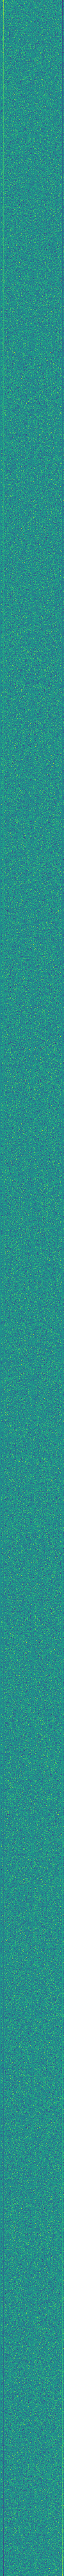
\includegraphics[interpolate=false,width=1.000000in,height=1.000000in]{antiderivative_ci_5-img0.png}}%
\end{pgfscope}%
\begin{pgfscope}%
\pgfsetbuttcap%
\pgfsetroundjoin%
\definecolor{currentfill}{rgb}{0.000000,0.000000,0.000000}%
\pgfsetfillcolor{currentfill}%
\pgfsetlinewidth{0.803000pt}%
\definecolor{currentstroke}{rgb}{0.000000,0.000000,0.000000}%
\pgfsetstrokecolor{currentstroke}%
\pgfsetdash{}{0pt}%
\pgfsys@defobject{currentmarker}{\pgfqpoint{0.000000in}{-0.048611in}}{\pgfqpoint{0.000000in}{0.000000in}}{%
\pgfpathmoveto{\pgfqpoint{0.000000in}{0.000000in}}%
\pgfpathlineto{\pgfqpoint{0.000000in}{-0.048611in}}%
\pgfusepath{stroke,fill}%
}%
\begin{pgfscope}%
\pgfsys@transformshift{0.779897in}{0.517039in}%
\pgfsys@useobject{currentmarker}{}%
\end{pgfscope}%
\end{pgfscope}%
\begin{pgfscope}%
\definecolor{textcolor}{rgb}{0.000000,0.000000,0.000000}%
\pgfsetstrokecolor{textcolor}%
\pgfsetfillcolor{textcolor}%
\pgftext[x=0.779897in,y=0.419816in,,top]{\color{textcolor}{\rmfamily\fontsize{12.000000}{14.400000}\selectfont\catcode`\^=\active\def^{\ifmmode\sp\else\^{}\fi}\catcode`\%=\active\def%{\%}0}}%
\end{pgfscope}%
\begin{pgfscope}%
\pgfsetbuttcap%
\pgfsetroundjoin%
\definecolor{currentfill}{rgb}{0.000000,0.000000,0.000000}%
\pgfsetfillcolor{currentfill}%
\pgfsetlinewidth{0.803000pt}%
\definecolor{currentstroke}{rgb}{0.000000,0.000000,0.000000}%
\pgfsetstrokecolor{currentstroke}%
\pgfsetdash{}{0pt}%
\pgfsys@defobject{currentmarker}{\pgfqpoint{0.000000in}{-0.048611in}}{\pgfqpoint{0.000000in}{0.000000in}}{%
\pgfpathmoveto{\pgfqpoint{0.000000in}{0.000000in}}%
\pgfpathlineto{\pgfqpoint{0.000000in}{-0.048611in}}%
\pgfusepath{stroke,fill}%
}%
\begin{pgfscope}%
\pgfsys@transformshift{1.693017in}{0.517039in}%
\pgfsys@useobject{currentmarker}{}%
\end{pgfscope}%
\end{pgfscope}%
\begin{pgfscope}%
\definecolor{textcolor}{rgb}{0.000000,0.000000,0.000000}%
\pgfsetstrokecolor{textcolor}%
\pgfsetfillcolor{textcolor}%
\pgftext[x=1.693017in,y=0.419816in,,top]{\color{textcolor}{\rmfamily\fontsize{12.000000}{14.400000}\selectfont\catcode`\^=\active\def^{\ifmmode\sp\else\^{}\fi}\catcode`\%=\active\def%{\%}20}}%
\end{pgfscope}%
\begin{pgfscope}%
\pgfsetbuttcap%
\pgfsetroundjoin%
\definecolor{currentfill}{rgb}{0.000000,0.000000,0.000000}%
\pgfsetfillcolor{currentfill}%
\pgfsetlinewidth{0.803000pt}%
\definecolor{currentstroke}{rgb}{0.000000,0.000000,0.000000}%
\pgfsetstrokecolor{currentstroke}%
\pgfsetdash{}{0pt}%
\pgfsys@defobject{currentmarker}{\pgfqpoint{0.000000in}{-0.048611in}}{\pgfqpoint{0.000000in}{0.000000in}}{%
\pgfpathmoveto{\pgfqpoint{0.000000in}{0.000000in}}%
\pgfpathlineto{\pgfqpoint{0.000000in}{-0.048611in}}%
\pgfusepath{stroke,fill}%
}%
\begin{pgfscope}%
\pgfsys@transformshift{2.606137in}{0.517039in}%
\pgfsys@useobject{currentmarker}{}%
\end{pgfscope}%
\end{pgfscope}%
\begin{pgfscope}%
\definecolor{textcolor}{rgb}{0.000000,0.000000,0.000000}%
\pgfsetstrokecolor{textcolor}%
\pgfsetfillcolor{textcolor}%
\pgftext[x=2.606137in,y=0.419816in,,top]{\color{textcolor}{\rmfamily\fontsize{12.000000}{14.400000}\selectfont\catcode`\^=\active\def^{\ifmmode\sp\else\^{}\fi}\catcode`\%=\active\def%{\%}40}}%
\end{pgfscope}%
\begin{pgfscope}%
\definecolor{textcolor}{rgb}{0.000000,0.000000,0.000000}%
\pgfsetstrokecolor{textcolor}%
\pgfsetfillcolor{textcolor}%
\pgftext[x=1.921297in,y=0.202965in,,top]{\color{textcolor}{\rmfamily\fontsize{12.000000}{14.400000}\selectfont\catcode`\^=\active\def^{\ifmmode\sp\else\^{}\fi}\catcode`\%=\active\def%{\%}input coefficients}}%
\end{pgfscope}%
\begin{pgfscope}%
\pgfsetbuttcap%
\pgfsetroundjoin%
\definecolor{currentfill}{rgb}{0.000000,0.000000,0.000000}%
\pgfsetfillcolor{currentfill}%
\pgfsetlinewidth{0.803000pt}%
\definecolor{currentstroke}{rgb}{0.000000,0.000000,0.000000}%
\pgfsetstrokecolor{currentstroke}%
\pgfsetdash{}{0pt}%
\pgfsys@defobject{currentmarker}{\pgfqpoint{-0.048611in}{0.000000in}}{\pgfqpoint{-0.000000in}{0.000000in}}{%
\pgfpathmoveto{\pgfqpoint{-0.000000in}{0.000000in}}%
\pgfpathlineto{\pgfqpoint{-0.048611in}{0.000000in}}%
\pgfusepath{stroke,fill}%
}%
\begin{pgfscope}%
\pgfsys@transformshift{0.779897in}{2.895016in}%
\pgfsys@useobject{currentmarker}{}%
\end{pgfscope}%
\end{pgfscope}%
\begin{pgfscope}%
\definecolor{textcolor}{rgb}{0.000000,0.000000,0.000000}%
\pgfsetstrokecolor{textcolor}%
\pgfsetfillcolor{textcolor}%
\pgftext[x=0.576636in, y=2.831702in, left, base]{\color{textcolor}{\rmfamily\fontsize{12.000000}{14.400000}\selectfont\catcode`\^=\active\def^{\ifmmode\sp\else\^{}\fi}\catcode`\%=\active\def%{\%}0}}%
\end{pgfscope}%
\begin{pgfscope}%
\pgfsetbuttcap%
\pgfsetroundjoin%
\definecolor{currentfill}{rgb}{0.000000,0.000000,0.000000}%
\pgfsetfillcolor{currentfill}%
\pgfsetlinewidth{0.803000pt}%
\definecolor{currentstroke}{rgb}{0.000000,0.000000,0.000000}%
\pgfsetstrokecolor{currentstroke}%
\pgfsetdash{}{0pt}%
\pgfsys@defobject{currentmarker}{\pgfqpoint{-0.048611in}{0.000000in}}{\pgfqpoint{-0.000000in}{0.000000in}}{%
\pgfpathmoveto{\pgfqpoint{-0.000000in}{0.000000in}}%
\pgfpathlineto{\pgfqpoint{-0.048611in}{0.000000in}}%
\pgfusepath{stroke,fill}%
}%
\begin{pgfscope}%
\pgfsys@transformshift{0.779897in}{2.300522in}%
\pgfsys@useobject{currentmarker}{}%
\end{pgfscope}%
\end{pgfscope}%
\begin{pgfscope}%
\definecolor{textcolor}{rgb}{0.000000,0.000000,0.000000}%
\pgfsetstrokecolor{textcolor}%
\pgfsetfillcolor{textcolor}%
\pgftext[x=0.258521in, y=2.237208in, left, base]{\color{textcolor}{\rmfamily\fontsize{12.000000}{14.400000}\selectfont\catcode`\^=\active\def^{\ifmmode\sp\else\^{}\fi}\catcode`\%=\active\def%{\%}1000}}%
\end{pgfscope}%
\begin{pgfscope}%
\pgfsetbuttcap%
\pgfsetroundjoin%
\definecolor{currentfill}{rgb}{0.000000,0.000000,0.000000}%
\pgfsetfillcolor{currentfill}%
\pgfsetlinewidth{0.803000pt}%
\definecolor{currentstroke}{rgb}{0.000000,0.000000,0.000000}%
\pgfsetstrokecolor{currentstroke}%
\pgfsetdash{}{0pt}%
\pgfsys@defobject{currentmarker}{\pgfqpoint{-0.048611in}{0.000000in}}{\pgfqpoint{-0.000000in}{0.000000in}}{%
\pgfpathmoveto{\pgfqpoint{-0.000000in}{0.000000in}}%
\pgfpathlineto{\pgfqpoint{-0.048611in}{0.000000in}}%
\pgfusepath{stroke,fill}%
}%
\begin{pgfscope}%
\pgfsys@transformshift{0.779897in}{1.706027in}%
\pgfsys@useobject{currentmarker}{}%
\end{pgfscope}%
\end{pgfscope}%
\begin{pgfscope}%
\definecolor{textcolor}{rgb}{0.000000,0.000000,0.000000}%
\pgfsetstrokecolor{textcolor}%
\pgfsetfillcolor{textcolor}%
\pgftext[x=0.258521in, y=1.642714in, left, base]{\color{textcolor}{\rmfamily\fontsize{12.000000}{14.400000}\selectfont\catcode`\^=\active\def^{\ifmmode\sp\else\^{}\fi}\catcode`\%=\active\def%{\%}2000}}%
\end{pgfscope}%
\begin{pgfscope}%
\pgfsetbuttcap%
\pgfsetroundjoin%
\definecolor{currentfill}{rgb}{0.000000,0.000000,0.000000}%
\pgfsetfillcolor{currentfill}%
\pgfsetlinewidth{0.803000pt}%
\definecolor{currentstroke}{rgb}{0.000000,0.000000,0.000000}%
\pgfsetstrokecolor{currentstroke}%
\pgfsetdash{}{0pt}%
\pgfsys@defobject{currentmarker}{\pgfqpoint{-0.048611in}{0.000000in}}{\pgfqpoint{-0.000000in}{0.000000in}}{%
\pgfpathmoveto{\pgfqpoint{-0.000000in}{0.000000in}}%
\pgfpathlineto{\pgfqpoint{-0.048611in}{0.000000in}}%
\pgfusepath{stroke,fill}%
}%
\begin{pgfscope}%
\pgfsys@transformshift{0.779897in}{1.111533in}%
\pgfsys@useobject{currentmarker}{}%
\end{pgfscope}%
\end{pgfscope}%
\begin{pgfscope}%
\definecolor{textcolor}{rgb}{0.000000,0.000000,0.000000}%
\pgfsetstrokecolor{textcolor}%
\pgfsetfillcolor{textcolor}%
\pgftext[x=0.258521in, y=1.048219in, left, base]{\color{textcolor}{\rmfamily\fontsize{12.000000}{14.400000}\selectfont\catcode`\^=\active\def^{\ifmmode\sp\else\^{}\fi}\catcode`\%=\active\def%{\%}3000}}%
\end{pgfscope}%
\begin{pgfscope}%
\pgfsetbuttcap%
\pgfsetroundjoin%
\definecolor{currentfill}{rgb}{0.000000,0.000000,0.000000}%
\pgfsetfillcolor{currentfill}%
\pgfsetlinewidth{0.803000pt}%
\definecolor{currentstroke}{rgb}{0.000000,0.000000,0.000000}%
\pgfsetstrokecolor{currentstroke}%
\pgfsetdash{}{0pt}%
\pgfsys@defobject{currentmarker}{\pgfqpoint{-0.048611in}{0.000000in}}{\pgfqpoint{-0.000000in}{0.000000in}}{%
\pgfpathmoveto{\pgfqpoint{-0.000000in}{0.000000in}}%
\pgfpathlineto{\pgfqpoint{-0.048611in}{0.000000in}}%
\pgfusepath{stroke,fill}%
}%
\begin{pgfscope}%
\pgfsys@transformshift{0.779897in}{0.517039in}%
\pgfsys@useobject{currentmarker}{}%
\end{pgfscope}%
\end{pgfscope}%
\begin{pgfscope}%
\definecolor{textcolor}{rgb}{0.000000,0.000000,0.000000}%
\pgfsetstrokecolor{textcolor}%
\pgfsetfillcolor{textcolor}%
\pgftext[x=0.258521in, y=0.453725in, left, base]{\color{textcolor}{\rmfamily\fontsize{12.000000}{14.400000}\selectfont\catcode`\^=\active\def^{\ifmmode\sp\else\^{}\fi}\catcode`\%=\active\def%{\%}4000}}%
\end{pgfscope}%
\begin{pgfscope}%
\definecolor{textcolor}{rgb}{0.000000,0.000000,0.000000}%
\pgfsetstrokecolor{textcolor}%
\pgfsetfillcolor{textcolor}%
\pgftext[x=0.202965in,y=1.706027in,,bottom,rotate=90.000000]{\color{textcolor}{\rmfamily\fontsize{12.000000}{14.400000}\selectfont\catcode`\^=\active\def^{\ifmmode\sp\else\^{}\fi}\catcode`\%=\active\def%{\%}samples}}%
\end{pgfscope}%
\begin{pgfscope}%
\pgfsetrectcap%
\pgfsetmiterjoin%
\pgfsetlinewidth{0.803000pt}%
\definecolor{currentstroke}{rgb}{0.000000,0.000000,0.000000}%
\pgfsetstrokecolor{currentstroke}%
\pgfsetdash{}{0pt}%
\pgfpathmoveto{\pgfqpoint{0.779897in}{0.517039in}}%
\pgfpathlineto{\pgfqpoint{0.779897in}{2.895016in}}%
\pgfusepath{stroke}%
\end{pgfscope}%
\begin{pgfscope}%
\pgfsetrectcap%
\pgfsetmiterjoin%
\pgfsetlinewidth{0.803000pt}%
\definecolor{currentstroke}{rgb}{0.000000,0.000000,0.000000}%
\pgfsetstrokecolor{currentstroke}%
\pgfsetdash{}{0pt}%
\pgfpathmoveto{\pgfqpoint{3.062697in}{0.517039in}}%
\pgfpathlineto{\pgfqpoint{3.062697in}{2.895016in}}%
\pgfusepath{stroke}%
\end{pgfscope}%
\begin{pgfscope}%
\pgfsetrectcap%
\pgfsetmiterjoin%
\pgfsetlinewidth{0.803000pt}%
\definecolor{currentstroke}{rgb}{0.000000,0.000000,0.000000}%
\pgfsetstrokecolor{currentstroke}%
\pgfsetdash{}{0pt}%
\pgfpathmoveto{\pgfqpoint{0.779897in}{0.517039in}}%
\pgfpathlineto{\pgfqpoint{3.062697in}{0.517039in}}%
\pgfusepath{stroke}%
\end{pgfscope}%
\begin{pgfscope}%
\pgfsetrectcap%
\pgfsetmiterjoin%
\pgfsetlinewidth{0.803000pt}%
\definecolor{currentstroke}{rgb}{0.000000,0.000000,0.000000}%
\pgfsetstrokecolor{currentstroke}%
\pgfsetdash{}{0pt}%
\pgfpathmoveto{\pgfqpoint{0.779897in}{2.895016in}}%
\pgfpathlineto{\pgfqpoint{3.062697in}{2.895016in}}%
\pgfusepath{stroke}%
\end{pgfscope}%
\begin{pgfscope}%
\pgfsetbuttcap%
\pgfsetmiterjoin%
\pgfsetlinewidth{0.000000pt}%
\definecolor{currentstroke}{rgb}{0.000000,0.000000,0.000000}%
\pgfsetstrokecolor{currentstroke}%
\pgfsetstrokeopacity{0.000000}%
\pgfsetdash{}{0pt}%
\pgfpathmoveto{\pgfqpoint{3.282875in}{0.517039in}}%
\pgfpathlineto{\pgfqpoint{3.401774in}{0.517039in}}%
\pgfpathlineto{\pgfqpoint{3.401774in}{2.895016in}}%
\pgfpathlineto{\pgfqpoint{3.282875in}{2.895016in}}%
\pgfpathlineto{\pgfqpoint{3.282875in}{0.517039in}}%
\pgfpathclose%
\pgfusepath{}%
\end{pgfscope}%
\begin{pgfscope}%
\pgfsys@transformshift{3.280000in}{0.520000in}%
\pgftext[left,bottom]{
\includegraphics[interpolate=true,width=0.120000in,height=2.380000in]{antiderivative_ci_5-img1.png}}%
\end{pgfscope}%
\begin{pgfscope}%
\pgfsetbuttcap%
\pgfsetroundjoin%
\definecolor{currentfill}{rgb}{0.000000,0.000000,0.000000}%
\pgfsetfillcolor{currentfill}%
\pgfsetlinewidth{0.803000pt}%
\definecolor{currentstroke}{rgb}{0.000000,0.000000,0.000000}%
\pgfsetstrokecolor{currentstroke}%
\pgfsetdash{}{0pt}%
\pgfsys@defobject{currentmarker}{\pgfqpoint{0.000000in}{0.000000in}}{\pgfqpoint{0.048611in}{0.000000in}}{%
\pgfpathmoveto{\pgfqpoint{0.000000in}{0.000000in}}%
\pgfpathlineto{\pgfqpoint{0.048611in}{0.000000in}}%
\pgfusepath{stroke,fill}%
}%
\begin{pgfscope}%
\pgfsys@transformshift{3.401774in}{0.636505in}%
\pgfsys@useobject{currentmarker}{}%
\end{pgfscope}%
\end{pgfscope}%
\begin{pgfscope}%
\definecolor{textcolor}{rgb}{0.000000,0.000000,0.000000}%
\pgfsetstrokecolor{textcolor}%
\pgfsetfillcolor{textcolor}%
\pgftext[x=3.498996in, y=0.573191in, left, base]{\color{textcolor}{\rmfamily\fontsize{12.000000}{14.400000}\selectfont\catcode`\^=\active\def^{\ifmmode\sp\else\^{}\fi}\catcode`\%=\active\def%{\%}\ensuremath{-}100}}%
\end{pgfscope}%
\begin{pgfscope}%
\pgfsetbuttcap%
\pgfsetroundjoin%
\definecolor{currentfill}{rgb}{0.000000,0.000000,0.000000}%
\pgfsetfillcolor{currentfill}%
\pgfsetlinewidth{0.803000pt}%
\definecolor{currentstroke}{rgb}{0.000000,0.000000,0.000000}%
\pgfsetstrokecolor{currentstroke}%
\pgfsetdash{}{0pt}%
\pgfsys@defobject{currentmarker}{\pgfqpoint{0.000000in}{0.000000in}}{\pgfqpoint{0.048611in}{0.000000in}}{%
\pgfpathmoveto{\pgfqpoint{0.000000in}{0.000000in}}%
\pgfpathlineto{\pgfqpoint{0.048611in}{0.000000in}}%
\pgfusepath{stroke,fill}%
}%
\begin{pgfscope}%
\pgfsys@transformshift{3.401774in}{1.171266in}%
\pgfsys@useobject{currentmarker}{}%
\end{pgfscope}%
\end{pgfscope}%
\begin{pgfscope}%
\definecolor{textcolor}{rgb}{0.000000,0.000000,0.000000}%
\pgfsetstrokecolor{textcolor}%
\pgfsetfillcolor{textcolor}%
\pgftext[x=3.498996in, y=1.107952in, left, base]{\color{textcolor}{\rmfamily\fontsize{12.000000}{14.400000}\selectfont\catcode`\^=\active\def^{\ifmmode\sp\else\^{}\fi}\catcode`\%=\active\def%{\%}\ensuremath{-}50}}%
\end{pgfscope}%
\begin{pgfscope}%
\pgfsetbuttcap%
\pgfsetroundjoin%
\definecolor{currentfill}{rgb}{0.000000,0.000000,0.000000}%
\pgfsetfillcolor{currentfill}%
\pgfsetlinewidth{0.803000pt}%
\definecolor{currentstroke}{rgb}{0.000000,0.000000,0.000000}%
\pgfsetstrokecolor{currentstroke}%
\pgfsetdash{}{0pt}%
\pgfsys@defobject{currentmarker}{\pgfqpoint{0.000000in}{0.000000in}}{\pgfqpoint{0.048611in}{0.000000in}}{%
\pgfpathmoveto{\pgfqpoint{0.000000in}{0.000000in}}%
\pgfpathlineto{\pgfqpoint{0.048611in}{0.000000in}}%
\pgfusepath{stroke,fill}%
}%
\begin{pgfscope}%
\pgfsys@transformshift{3.401774in}{1.706028in}%
\pgfsys@useobject{currentmarker}{}%
\end{pgfscope}%
\end{pgfscope}%
\begin{pgfscope}%
\definecolor{textcolor}{rgb}{0.000000,0.000000,0.000000}%
\pgfsetstrokecolor{textcolor}%
\pgfsetfillcolor{textcolor}%
\pgftext[x=3.498996in, y=1.642714in, left, base]{\color{textcolor}{\rmfamily\fontsize{12.000000}{14.400000}\selectfont\catcode`\^=\active\def^{\ifmmode\sp\else\^{}\fi}\catcode`\%=\active\def%{\%}0}}%
\end{pgfscope}%
\begin{pgfscope}%
\pgfsetbuttcap%
\pgfsetroundjoin%
\definecolor{currentfill}{rgb}{0.000000,0.000000,0.000000}%
\pgfsetfillcolor{currentfill}%
\pgfsetlinewidth{0.803000pt}%
\definecolor{currentstroke}{rgb}{0.000000,0.000000,0.000000}%
\pgfsetstrokecolor{currentstroke}%
\pgfsetdash{}{0pt}%
\pgfsys@defobject{currentmarker}{\pgfqpoint{0.000000in}{0.000000in}}{\pgfqpoint{0.048611in}{0.000000in}}{%
\pgfpathmoveto{\pgfqpoint{0.000000in}{0.000000in}}%
\pgfpathlineto{\pgfqpoint{0.048611in}{0.000000in}}%
\pgfusepath{stroke,fill}%
}%
\begin{pgfscope}%
\pgfsys@transformshift{3.401774in}{2.240789in}%
\pgfsys@useobject{currentmarker}{}%
\end{pgfscope}%
\end{pgfscope}%
\begin{pgfscope}%
\definecolor{textcolor}{rgb}{0.000000,0.000000,0.000000}%
\pgfsetstrokecolor{textcolor}%
\pgfsetfillcolor{textcolor}%
\pgftext[x=3.498996in, y=2.177475in, left, base]{\color{textcolor}{\rmfamily\fontsize{12.000000}{14.400000}\selectfont\catcode`\^=\active\def^{\ifmmode\sp\else\^{}\fi}\catcode`\%=\active\def%{\%}50}}%
\end{pgfscope}%
\begin{pgfscope}%
\pgfsetbuttcap%
\pgfsetroundjoin%
\definecolor{currentfill}{rgb}{0.000000,0.000000,0.000000}%
\pgfsetfillcolor{currentfill}%
\pgfsetlinewidth{0.803000pt}%
\definecolor{currentstroke}{rgb}{0.000000,0.000000,0.000000}%
\pgfsetstrokecolor{currentstroke}%
\pgfsetdash{}{0pt}%
\pgfsys@defobject{currentmarker}{\pgfqpoint{0.000000in}{0.000000in}}{\pgfqpoint{0.048611in}{0.000000in}}{%
\pgfpathmoveto{\pgfqpoint{0.000000in}{0.000000in}}%
\pgfpathlineto{\pgfqpoint{0.048611in}{0.000000in}}%
\pgfusepath{stroke,fill}%
}%
\begin{pgfscope}%
\pgfsys@transformshift{3.401774in}{2.775550in}%
\pgfsys@useobject{currentmarker}{}%
\end{pgfscope}%
\end{pgfscope}%
\begin{pgfscope}%
\definecolor{textcolor}{rgb}{0.000000,0.000000,0.000000}%
\pgfsetstrokecolor{textcolor}%
\pgfsetfillcolor{textcolor}%
\pgftext[x=3.498996in, y=2.712237in, left, base]{\color{textcolor}{\rmfamily\fontsize{12.000000}{14.400000}\selectfont\catcode`\^=\active\def^{\ifmmode\sp\else\^{}\fi}\catcode`\%=\active\def%{\%}100}}%
\end{pgfscope}%
\begin{pgfscope}%
\pgfsetrectcap%
\pgfsetmiterjoin%
\pgfsetlinewidth{0.803000pt}%
\definecolor{currentstroke}{rgb}{0.000000,0.000000,0.000000}%
\pgfsetstrokecolor{currentstroke}%
\pgfsetdash{}{0pt}%
\pgfpathmoveto{\pgfqpoint{3.282875in}{0.517039in}}%
\pgfpathlineto{\pgfqpoint{3.342325in}{0.517039in}}%
\pgfpathlineto{\pgfqpoint{3.401774in}{0.517039in}}%
\pgfpathlineto{\pgfqpoint{3.401774in}{2.895016in}}%
\pgfpathlineto{\pgfqpoint{3.342325in}{2.895016in}}%
\pgfpathlineto{\pgfqpoint{3.282875in}{2.895016in}}%
\pgfpathlineto{\pgfqpoint{3.282875in}{0.517039in}}%
\pgfpathclose%
\pgfusepath{stroke}%
\end{pgfscope}%
\end{pgfpicture}%
\makeatother%
\endgroup%

      \end{adjustbox}
      \caption{Correlation image 5\% noise.}\label{fig:sc1_ci_5}
    \end{subfigure}
    \begin{subfigure}{0.49\linewidth}
      \begin{adjustbox}{width=\linewidth}
        \begingroup%
\makeatletter%
\begin{pgfpicture}%
\pgfpathrectangle{\pgfpointorigin}{\pgfqpoint{6.400000in}{4.800000in}}%
\pgfusepath{use as bounding box, clip}%
\begin{pgfscope}%
\pgfsetbuttcap%
\pgfsetmiterjoin%
\pgfsetlinewidth{0.000000pt}%
\definecolor{currentstroke}{rgb}{0.000000,0.000000,0.000000}%
\pgfsetstrokecolor{currentstroke}%
\pgfsetstrokeopacity{0.000000}%
\pgfsetdash{}{0pt}%
\pgfpathmoveto{\pgfqpoint{0.000000in}{0.000000in}}%
\pgfpathlineto{\pgfqpoint{6.400000in}{0.000000in}}%
\pgfpathlineto{\pgfqpoint{6.400000in}{4.800000in}}%
\pgfpathlineto{\pgfqpoint{0.000000in}{4.800000in}}%
\pgfpathlineto{\pgfqpoint{0.000000in}{0.000000in}}%
\pgfpathclose%
\pgfusepath{}%
\end{pgfscope}%
\begin{pgfscope}%
\pgfsetbuttcap%
\pgfsetmiterjoin%
\pgfsetlinewidth{0.000000pt}%
\definecolor{currentstroke}{rgb}{0.000000,0.000000,0.000000}%
\pgfsetstrokecolor{currentstroke}%
\pgfsetstrokeopacity{0.000000}%
\pgfsetdash{}{0pt}%
\pgfpathmoveto{\pgfqpoint{1.072000in}{0.528000in}}%
\pgfpathlineto{\pgfqpoint{4.768000in}{0.528000in}}%
\pgfpathlineto{\pgfqpoint{4.768000in}{4.224000in}}%
\pgfpathlineto{\pgfqpoint{1.072000in}{4.224000in}}%
\pgfpathlineto{\pgfqpoint{1.072000in}{0.528000in}}%
\pgfpathclose%
\pgfusepath{}%
\end{pgfscope}%
\begin{pgfscope}%
\pgfpathrectangle{\pgfqpoint{1.072000in}{0.528000in}}{\pgfqpoint{3.696000in}{3.696000in}}%
\pgfusepath{clip}%
\pgfsys@transformcm{3.696000}{0.000000}{0.000000}{-3.696000}{1.072000in}{4.224000in}%
\pgftext[left,bottom]{
\includegraphics[interpolate=false,width=1.000000in,height=1.000000in]{antiderivative_pm_5-img0.png}}%
\end{pgfscope}%
\begin{pgfscope}%
\pgfsetbuttcap%
\pgfsetroundjoin%
\definecolor{currentfill}{rgb}{0.000000,0.000000,0.000000}%
\pgfsetfillcolor{currentfill}%
\pgfsetlinewidth{0.803000pt}%
\definecolor{currentstroke}{rgb}{0.000000,0.000000,0.000000}%
\pgfsetstrokecolor{currentstroke}%
\pgfsetdash{}{0pt}%
\pgfsys@defobject{currentmarker}{\pgfqpoint{0.000000in}{-0.048611in}}{\pgfqpoint{0.000000in}{0.000000in}}{%
\pgfpathmoveto{\pgfqpoint{0.000000in}{0.000000in}}%
\pgfpathlineto{\pgfqpoint{0.000000in}{-0.048611in}}%
\pgfusepath{stroke,fill}%
}%
\begin{pgfscope}%
\pgfsys@transformshift{1.090480in}{0.528000in}%
\pgfsys@useobject{currentmarker}{}%
\end{pgfscope}%
\end{pgfscope}%
\begin{pgfscope}%
\definecolor{textcolor}{rgb}{0.000000,0.000000,0.000000}%
\pgfsetstrokecolor{textcolor}%
\pgfsetfillcolor{textcolor}%
\pgftext[x=1.090480in,y=0.430778in,,top]{\color{textcolor}{\rmfamily\fontsize{12.000000}{14.400000}\selectfont\catcode`\^=\active\def^{\ifmmode\sp\else\^{}\fi}\catcode`\%=\active\def%{\%}0}}%
\end{pgfscope}%
\begin{pgfscope}%
\pgfsetbuttcap%
\pgfsetroundjoin%
\definecolor{currentfill}{rgb}{0.000000,0.000000,0.000000}%
\pgfsetfillcolor{currentfill}%
\pgfsetlinewidth{0.803000pt}%
\definecolor{currentstroke}{rgb}{0.000000,0.000000,0.000000}%
\pgfsetstrokecolor{currentstroke}%
\pgfsetdash{}{0pt}%
\pgfsys@defobject{currentmarker}{\pgfqpoint{0.000000in}{-0.048611in}}{\pgfqpoint{0.000000in}{0.000000in}}{%
\pgfpathmoveto{\pgfqpoint{0.000000in}{0.000000in}}%
\pgfpathlineto{\pgfqpoint{0.000000in}{-0.048611in}}%
\pgfusepath{stroke,fill}%
}%
\begin{pgfscope}%
\pgfsys@transformshift{1.829680in}{0.528000in}%
\pgfsys@useobject{currentmarker}{}%
\end{pgfscope}%
\end{pgfscope}%
\begin{pgfscope}%
\definecolor{textcolor}{rgb}{0.000000,0.000000,0.000000}%
\pgfsetstrokecolor{textcolor}%
\pgfsetfillcolor{textcolor}%
\pgftext[x=1.829680in,y=0.430778in,,top]{\color{textcolor}{\rmfamily\fontsize{12.000000}{14.400000}\selectfont\catcode`\^=\active\def^{\ifmmode\sp\else\^{}\fi}\catcode`\%=\active\def%{\%}20}}%
\end{pgfscope}%
\begin{pgfscope}%
\pgfsetbuttcap%
\pgfsetroundjoin%
\definecolor{currentfill}{rgb}{0.000000,0.000000,0.000000}%
\pgfsetfillcolor{currentfill}%
\pgfsetlinewidth{0.803000pt}%
\definecolor{currentstroke}{rgb}{0.000000,0.000000,0.000000}%
\pgfsetstrokecolor{currentstroke}%
\pgfsetdash{}{0pt}%
\pgfsys@defobject{currentmarker}{\pgfqpoint{0.000000in}{-0.048611in}}{\pgfqpoint{0.000000in}{0.000000in}}{%
\pgfpathmoveto{\pgfqpoint{0.000000in}{0.000000in}}%
\pgfpathlineto{\pgfqpoint{0.000000in}{-0.048611in}}%
\pgfusepath{stroke,fill}%
}%
\begin{pgfscope}%
\pgfsys@transformshift{2.568880in}{0.528000in}%
\pgfsys@useobject{currentmarker}{}%
\end{pgfscope}%
\end{pgfscope}%
\begin{pgfscope}%
\definecolor{textcolor}{rgb}{0.000000,0.000000,0.000000}%
\pgfsetstrokecolor{textcolor}%
\pgfsetfillcolor{textcolor}%
\pgftext[x=2.568880in,y=0.430778in,,top]{\color{textcolor}{\rmfamily\fontsize{12.000000}{14.400000}\selectfont\catcode`\^=\active\def^{\ifmmode\sp\else\^{}\fi}\catcode`\%=\active\def%{\%}40}}%
\end{pgfscope}%
\begin{pgfscope}%
\pgfsetbuttcap%
\pgfsetroundjoin%
\definecolor{currentfill}{rgb}{0.000000,0.000000,0.000000}%
\pgfsetfillcolor{currentfill}%
\pgfsetlinewidth{0.803000pt}%
\definecolor{currentstroke}{rgb}{0.000000,0.000000,0.000000}%
\pgfsetstrokecolor{currentstroke}%
\pgfsetdash{}{0pt}%
\pgfsys@defobject{currentmarker}{\pgfqpoint{0.000000in}{-0.048611in}}{\pgfqpoint{0.000000in}{0.000000in}}{%
\pgfpathmoveto{\pgfqpoint{0.000000in}{0.000000in}}%
\pgfpathlineto{\pgfqpoint{0.000000in}{-0.048611in}}%
\pgfusepath{stroke,fill}%
}%
\begin{pgfscope}%
\pgfsys@transformshift{3.308080in}{0.528000in}%
\pgfsys@useobject{currentmarker}{}%
\end{pgfscope}%
\end{pgfscope}%
\begin{pgfscope}%
\definecolor{textcolor}{rgb}{0.000000,0.000000,0.000000}%
\pgfsetstrokecolor{textcolor}%
\pgfsetfillcolor{textcolor}%
\pgftext[x=3.308080in,y=0.430778in,,top]{\color{textcolor}{\rmfamily\fontsize{12.000000}{14.400000}\selectfont\catcode`\^=\active\def^{\ifmmode\sp\else\^{}\fi}\catcode`\%=\active\def%{\%}60}}%
\end{pgfscope}%
\begin{pgfscope}%
\pgfsetbuttcap%
\pgfsetroundjoin%
\definecolor{currentfill}{rgb}{0.000000,0.000000,0.000000}%
\pgfsetfillcolor{currentfill}%
\pgfsetlinewidth{0.803000pt}%
\definecolor{currentstroke}{rgb}{0.000000,0.000000,0.000000}%
\pgfsetstrokecolor{currentstroke}%
\pgfsetdash{}{0pt}%
\pgfsys@defobject{currentmarker}{\pgfqpoint{0.000000in}{-0.048611in}}{\pgfqpoint{0.000000in}{0.000000in}}{%
\pgfpathmoveto{\pgfqpoint{0.000000in}{0.000000in}}%
\pgfpathlineto{\pgfqpoint{0.000000in}{-0.048611in}}%
\pgfusepath{stroke,fill}%
}%
\begin{pgfscope}%
\pgfsys@transformshift{4.047280in}{0.528000in}%
\pgfsys@useobject{currentmarker}{}%
\end{pgfscope}%
\end{pgfscope}%
\begin{pgfscope}%
\definecolor{textcolor}{rgb}{0.000000,0.000000,0.000000}%
\pgfsetstrokecolor{textcolor}%
\pgfsetfillcolor{textcolor}%
\pgftext[x=4.047280in,y=0.430778in,,top]{\color{textcolor}{\rmfamily\fontsize{12.000000}{14.400000}\selectfont\catcode`\^=\active\def^{\ifmmode\sp\else\^{}\fi}\catcode`\%=\active\def%{\%}80}}%
\end{pgfscope}%
\begin{pgfscope}%
\definecolor{textcolor}{rgb}{0.000000,0.000000,0.000000}%
\pgfsetstrokecolor{textcolor}%
\pgfsetfillcolor{textcolor}%
\pgftext[x=2.920000in,y=0.213927in,,top]{\color{textcolor}{\rmfamily\fontsize{12.000000}{14.400000}\selectfont\catcode`\^=\active\def^{\ifmmode\sp\else\^{}\fi}\catcode`\%=\active\def%{\%}output coefficients}}%
\end{pgfscope}%
\begin{pgfscope}%
\pgfsetbuttcap%
\pgfsetroundjoin%
\definecolor{currentfill}{rgb}{0.000000,0.000000,0.000000}%
\pgfsetfillcolor{currentfill}%
\pgfsetlinewidth{0.803000pt}%
\definecolor{currentstroke}{rgb}{0.000000,0.000000,0.000000}%
\pgfsetstrokecolor{currentstroke}%
\pgfsetdash{}{0pt}%
\pgfsys@defobject{currentmarker}{\pgfqpoint{-0.048611in}{0.000000in}}{\pgfqpoint{-0.000000in}{0.000000in}}{%
\pgfpathmoveto{\pgfqpoint{-0.000000in}{0.000000in}}%
\pgfpathlineto{\pgfqpoint{-0.048611in}{0.000000in}}%
\pgfusepath{stroke,fill}%
}%
\begin{pgfscope}%
\pgfsys@transformshift{1.072000in}{4.205520in}%
\pgfsys@useobject{currentmarker}{}%
\end{pgfscope}%
\end{pgfscope}%
\begin{pgfscope}%
\definecolor{textcolor}{rgb}{0.000000,0.000000,0.000000}%
\pgfsetstrokecolor{textcolor}%
\pgfsetfillcolor{textcolor}%
\pgftext[x=0.868739in, y=4.142206in, left, base]{\color{textcolor}{\rmfamily\fontsize{12.000000}{14.400000}\selectfont\catcode`\^=\active\def^{\ifmmode\sp\else\^{}\fi}\catcode`\%=\active\def%{\%}0}}%
\end{pgfscope}%
\begin{pgfscope}%
\pgfsetbuttcap%
\pgfsetroundjoin%
\definecolor{currentfill}{rgb}{0.000000,0.000000,0.000000}%
\pgfsetfillcolor{currentfill}%
\pgfsetlinewidth{0.803000pt}%
\definecolor{currentstroke}{rgb}{0.000000,0.000000,0.000000}%
\pgfsetstrokecolor{currentstroke}%
\pgfsetdash{}{0pt}%
\pgfsys@defobject{currentmarker}{\pgfqpoint{-0.048611in}{0.000000in}}{\pgfqpoint{-0.000000in}{0.000000in}}{%
\pgfpathmoveto{\pgfqpoint{-0.000000in}{0.000000in}}%
\pgfpathlineto{\pgfqpoint{-0.048611in}{0.000000in}}%
\pgfusepath{stroke,fill}%
}%
\begin{pgfscope}%
\pgfsys@transformshift{1.072000in}{3.466320in}%
\pgfsys@useobject{currentmarker}{}%
\end{pgfscope}%
\end{pgfscope}%
\begin{pgfscope}%
\definecolor{textcolor}{rgb}{0.000000,0.000000,0.000000}%
\pgfsetstrokecolor{textcolor}%
\pgfsetfillcolor{textcolor}%
\pgftext[x=0.762701in, y=3.403006in, left, base]{\color{textcolor}{\rmfamily\fontsize{12.000000}{14.400000}\selectfont\catcode`\^=\active\def^{\ifmmode\sp\else\^{}\fi}\catcode`\%=\active\def%{\%}20}}%
\end{pgfscope}%
\begin{pgfscope}%
\pgfsetbuttcap%
\pgfsetroundjoin%
\definecolor{currentfill}{rgb}{0.000000,0.000000,0.000000}%
\pgfsetfillcolor{currentfill}%
\pgfsetlinewidth{0.803000pt}%
\definecolor{currentstroke}{rgb}{0.000000,0.000000,0.000000}%
\pgfsetstrokecolor{currentstroke}%
\pgfsetdash{}{0pt}%
\pgfsys@defobject{currentmarker}{\pgfqpoint{-0.048611in}{0.000000in}}{\pgfqpoint{-0.000000in}{0.000000in}}{%
\pgfpathmoveto{\pgfqpoint{-0.000000in}{0.000000in}}%
\pgfpathlineto{\pgfqpoint{-0.048611in}{0.000000in}}%
\pgfusepath{stroke,fill}%
}%
\begin{pgfscope}%
\pgfsys@transformshift{1.072000in}{2.727120in}%
\pgfsys@useobject{currentmarker}{}%
\end{pgfscope}%
\end{pgfscope}%
\begin{pgfscope}%
\definecolor{textcolor}{rgb}{0.000000,0.000000,0.000000}%
\pgfsetstrokecolor{textcolor}%
\pgfsetfillcolor{textcolor}%
\pgftext[x=0.762701in, y=2.663806in, left, base]{\color{textcolor}{\rmfamily\fontsize{12.000000}{14.400000}\selectfont\catcode`\^=\active\def^{\ifmmode\sp\else\^{}\fi}\catcode`\%=\active\def%{\%}40}}%
\end{pgfscope}%
\begin{pgfscope}%
\pgfsetbuttcap%
\pgfsetroundjoin%
\definecolor{currentfill}{rgb}{0.000000,0.000000,0.000000}%
\pgfsetfillcolor{currentfill}%
\pgfsetlinewidth{0.803000pt}%
\definecolor{currentstroke}{rgb}{0.000000,0.000000,0.000000}%
\pgfsetstrokecolor{currentstroke}%
\pgfsetdash{}{0pt}%
\pgfsys@defobject{currentmarker}{\pgfqpoint{-0.048611in}{0.000000in}}{\pgfqpoint{-0.000000in}{0.000000in}}{%
\pgfpathmoveto{\pgfqpoint{-0.000000in}{0.000000in}}%
\pgfpathlineto{\pgfqpoint{-0.048611in}{0.000000in}}%
\pgfusepath{stroke,fill}%
}%
\begin{pgfscope}%
\pgfsys@transformshift{1.072000in}{1.987920in}%
\pgfsys@useobject{currentmarker}{}%
\end{pgfscope}%
\end{pgfscope}%
\begin{pgfscope}%
\definecolor{textcolor}{rgb}{0.000000,0.000000,0.000000}%
\pgfsetstrokecolor{textcolor}%
\pgfsetfillcolor{textcolor}%
\pgftext[x=0.762701in, y=1.924606in, left, base]{\color{textcolor}{\rmfamily\fontsize{12.000000}{14.400000}\selectfont\catcode`\^=\active\def^{\ifmmode\sp\else\^{}\fi}\catcode`\%=\active\def%{\%}60}}%
\end{pgfscope}%
\begin{pgfscope}%
\pgfsetbuttcap%
\pgfsetroundjoin%
\definecolor{currentfill}{rgb}{0.000000,0.000000,0.000000}%
\pgfsetfillcolor{currentfill}%
\pgfsetlinewidth{0.803000pt}%
\definecolor{currentstroke}{rgb}{0.000000,0.000000,0.000000}%
\pgfsetstrokecolor{currentstroke}%
\pgfsetdash{}{0pt}%
\pgfsys@defobject{currentmarker}{\pgfqpoint{-0.048611in}{0.000000in}}{\pgfqpoint{-0.000000in}{0.000000in}}{%
\pgfpathmoveto{\pgfqpoint{-0.000000in}{0.000000in}}%
\pgfpathlineto{\pgfqpoint{-0.048611in}{0.000000in}}%
\pgfusepath{stroke,fill}%
}%
\begin{pgfscope}%
\pgfsys@transformshift{1.072000in}{1.248720in}%
\pgfsys@useobject{currentmarker}{}%
\end{pgfscope}%
\end{pgfscope}%
\begin{pgfscope}%
\definecolor{textcolor}{rgb}{0.000000,0.000000,0.000000}%
\pgfsetstrokecolor{textcolor}%
\pgfsetfillcolor{textcolor}%
\pgftext[x=0.762701in, y=1.185406in, left, base]{\color{textcolor}{\rmfamily\fontsize{12.000000}{14.400000}\selectfont\catcode`\^=\active\def^{\ifmmode\sp\else\^{}\fi}\catcode`\%=\active\def%{\%}80}}%
\end{pgfscope}%
\begin{pgfscope}%
\definecolor{textcolor}{rgb}{0.000000,0.000000,0.000000}%
\pgfsetstrokecolor{textcolor}%
\pgfsetfillcolor{textcolor}%
\pgftext[x=0.707145in,y=2.376000in,,bottom,rotate=90.000000]{\color{textcolor}{\rmfamily\fontsize{12.000000}{14.400000}\selectfont\catcode`\^=\active\def^{\ifmmode\sp\else\^{}\fi}\catcode`\%=\active\def%{\%}input coefficients}}%
\end{pgfscope}%
\begin{pgfscope}%
\pgfsetrectcap%
\pgfsetmiterjoin%
\pgfsetlinewidth{0.803000pt}%
\definecolor{currentstroke}{rgb}{0.000000,0.000000,0.000000}%
\pgfsetstrokecolor{currentstroke}%
\pgfsetdash{}{0pt}%
\pgfpathmoveto{\pgfqpoint{1.072000in}{0.528000in}}%
\pgfpathlineto{\pgfqpoint{1.072000in}{4.224000in}}%
\pgfusepath{stroke}%
\end{pgfscope}%
\begin{pgfscope}%
\pgfsetrectcap%
\pgfsetmiterjoin%
\pgfsetlinewidth{0.803000pt}%
\definecolor{currentstroke}{rgb}{0.000000,0.000000,0.000000}%
\pgfsetstrokecolor{currentstroke}%
\pgfsetdash{}{0pt}%
\pgfpathmoveto{\pgfqpoint{4.768000in}{0.528000in}}%
\pgfpathlineto{\pgfqpoint{4.768000in}{4.224000in}}%
\pgfusepath{stroke}%
\end{pgfscope}%
\begin{pgfscope}%
\pgfsetrectcap%
\pgfsetmiterjoin%
\pgfsetlinewidth{0.803000pt}%
\definecolor{currentstroke}{rgb}{0.000000,0.000000,0.000000}%
\pgfsetstrokecolor{currentstroke}%
\pgfsetdash{}{0pt}%
\pgfpathmoveto{\pgfqpoint{1.072000in}{0.528000in}}%
\pgfpathlineto{\pgfqpoint{4.768000in}{0.528000in}}%
\pgfusepath{stroke}%
\end{pgfscope}%
\begin{pgfscope}%
\pgfsetrectcap%
\pgfsetmiterjoin%
\pgfsetlinewidth{0.803000pt}%
\definecolor{currentstroke}{rgb}{0.000000,0.000000,0.000000}%
\pgfsetstrokecolor{currentstroke}%
\pgfsetdash{}{0pt}%
\pgfpathmoveto{\pgfqpoint{1.072000in}{4.224000in}}%
\pgfpathlineto{\pgfqpoint{4.768000in}{4.224000in}}%
\pgfusepath{stroke}%
\end{pgfscope}%
\begin{pgfscope}%
\pgfsetbuttcap%
\pgfsetmiterjoin%
\pgfsetlinewidth{0.000000pt}%
\definecolor{currentstroke}{rgb}{0.000000,0.000000,0.000000}%
\pgfsetstrokecolor{currentstroke}%
\pgfsetstrokeopacity{0.000000}%
\pgfsetdash{}{0pt}%
\pgfpathmoveto{\pgfqpoint{5.016000in}{0.528000in}}%
\pgfpathlineto{\pgfqpoint{5.200800in}{0.528000in}}%
\pgfpathlineto{\pgfqpoint{5.200800in}{4.224000in}}%
\pgfpathlineto{\pgfqpoint{5.016000in}{4.224000in}}%
\pgfpathlineto{\pgfqpoint{5.016000in}{0.528000in}}%
\pgfpathclose%
\pgfusepath{}%
\end{pgfscope}%
\begin{pgfscope}%
\pgfsys@transformshift{5.020000in}{0.530000in}%
\pgftext[left,bottom]{
\includegraphics[interpolate=true,width=0.180000in,height=3.690000in]{antiderivative_pm_5-img1.png}}%
\end{pgfscope}%
\begin{pgfscope}%
\pgfsetbuttcap%
\pgfsetroundjoin%
\definecolor{currentfill}{rgb}{0.000000,0.000000,0.000000}%
\pgfsetfillcolor{currentfill}%
\pgfsetlinewidth{0.803000pt}%
\definecolor{currentstroke}{rgb}{0.000000,0.000000,0.000000}%
\pgfsetstrokecolor{currentstroke}%
\pgfsetdash{}{0pt}%
\pgfsys@defobject{currentmarker}{\pgfqpoint{0.000000in}{0.000000in}}{\pgfqpoint{0.048611in}{0.000000in}}{%
\pgfpathmoveto{\pgfqpoint{0.000000in}{0.000000in}}%
\pgfpathlineto{\pgfqpoint{0.048611in}{0.000000in}}%
\pgfusepath{stroke,fill}%
}%
\begin{pgfscope}%
\pgfsys@transformshift{5.200800in}{0.806760in}%
\pgfsys@useobject{currentmarker}{}%
\end{pgfscope}%
\end{pgfscope}%
\begin{pgfscope}%
\definecolor{textcolor}{rgb}{0.000000,0.000000,0.000000}%
\pgfsetstrokecolor{textcolor}%
\pgfsetfillcolor{textcolor}%
\pgftext[x=5.298022in, y=0.743447in, left, base]{\color{textcolor}{\rmfamily\fontsize{12.000000}{14.400000}\selectfont\catcode`\^=\active\def^{\ifmmode\sp\else\^{}\fi}\catcode`\%=\active\def%{\%}\ensuremath{-}2000}}%
\end{pgfscope}%
\begin{pgfscope}%
\pgfsetbuttcap%
\pgfsetroundjoin%
\definecolor{currentfill}{rgb}{0.000000,0.000000,0.000000}%
\pgfsetfillcolor{currentfill}%
\pgfsetlinewidth{0.803000pt}%
\definecolor{currentstroke}{rgb}{0.000000,0.000000,0.000000}%
\pgfsetstrokecolor{currentstroke}%
\pgfsetdash{}{0pt}%
\pgfsys@defobject{currentmarker}{\pgfqpoint{0.000000in}{0.000000in}}{\pgfqpoint{0.048611in}{0.000000in}}{%
\pgfpathmoveto{\pgfqpoint{0.000000in}{0.000000in}}%
\pgfpathlineto{\pgfqpoint{0.048611in}{0.000000in}}%
\pgfusepath{stroke,fill}%
}%
\begin{pgfscope}%
\pgfsys@transformshift{5.200800in}{1.404820in}%
\pgfsys@useobject{currentmarker}{}%
\end{pgfscope}%
\end{pgfscope}%
\begin{pgfscope}%
\definecolor{textcolor}{rgb}{0.000000,0.000000,0.000000}%
\pgfsetstrokecolor{textcolor}%
\pgfsetfillcolor{textcolor}%
\pgftext[x=5.298022in, y=1.341506in, left, base]{\color{textcolor}{\rmfamily\fontsize{12.000000}{14.400000}\selectfont\catcode`\^=\active\def^{\ifmmode\sp\else\^{}\fi}\catcode`\%=\active\def%{\%}\ensuremath{-}1500}}%
\end{pgfscope}%
\begin{pgfscope}%
\pgfsetbuttcap%
\pgfsetroundjoin%
\definecolor{currentfill}{rgb}{0.000000,0.000000,0.000000}%
\pgfsetfillcolor{currentfill}%
\pgfsetlinewidth{0.803000pt}%
\definecolor{currentstroke}{rgb}{0.000000,0.000000,0.000000}%
\pgfsetstrokecolor{currentstroke}%
\pgfsetdash{}{0pt}%
\pgfsys@defobject{currentmarker}{\pgfqpoint{0.000000in}{0.000000in}}{\pgfqpoint{0.048611in}{0.000000in}}{%
\pgfpathmoveto{\pgfqpoint{0.000000in}{0.000000in}}%
\pgfpathlineto{\pgfqpoint{0.048611in}{0.000000in}}%
\pgfusepath{stroke,fill}%
}%
\begin{pgfscope}%
\pgfsys@transformshift{5.200800in}{2.002880in}%
\pgfsys@useobject{currentmarker}{}%
\end{pgfscope}%
\end{pgfscope}%
\begin{pgfscope}%
\definecolor{textcolor}{rgb}{0.000000,0.000000,0.000000}%
\pgfsetstrokecolor{textcolor}%
\pgfsetfillcolor{textcolor}%
\pgftext[x=5.298022in, y=1.939566in, left, base]{\color{textcolor}{\rmfamily\fontsize{12.000000}{14.400000}\selectfont\catcode`\^=\active\def^{\ifmmode\sp\else\^{}\fi}\catcode`\%=\active\def%{\%}\ensuremath{-}1000}}%
\end{pgfscope}%
\begin{pgfscope}%
\pgfsetbuttcap%
\pgfsetroundjoin%
\definecolor{currentfill}{rgb}{0.000000,0.000000,0.000000}%
\pgfsetfillcolor{currentfill}%
\pgfsetlinewidth{0.803000pt}%
\definecolor{currentstroke}{rgb}{0.000000,0.000000,0.000000}%
\pgfsetstrokecolor{currentstroke}%
\pgfsetdash{}{0pt}%
\pgfsys@defobject{currentmarker}{\pgfqpoint{0.000000in}{0.000000in}}{\pgfqpoint{0.048611in}{0.000000in}}{%
\pgfpathmoveto{\pgfqpoint{0.000000in}{0.000000in}}%
\pgfpathlineto{\pgfqpoint{0.048611in}{0.000000in}}%
\pgfusepath{stroke,fill}%
}%
\begin{pgfscope}%
\pgfsys@transformshift{5.200800in}{2.600940in}%
\pgfsys@useobject{currentmarker}{}%
\end{pgfscope}%
\end{pgfscope}%
\begin{pgfscope}%
\definecolor{textcolor}{rgb}{0.000000,0.000000,0.000000}%
\pgfsetstrokecolor{textcolor}%
\pgfsetfillcolor{textcolor}%
\pgftext[x=5.298022in, y=2.537626in, left, base]{\color{textcolor}{\rmfamily\fontsize{12.000000}{14.400000}\selectfont\catcode`\^=\active\def^{\ifmmode\sp\else\^{}\fi}\catcode`\%=\active\def%{\%}\ensuremath{-}500}}%
\end{pgfscope}%
\begin{pgfscope}%
\pgfsetbuttcap%
\pgfsetroundjoin%
\definecolor{currentfill}{rgb}{0.000000,0.000000,0.000000}%
\pgfsetfillcolor{currentfill}%
\pgfsetlinewidth{0.803000pt}%
\definecolor{currentstroke}{rgb}{0.000000,0.000000,0.000000}%
\pgfsetstrokecolor{currentstroke}%
\pgfsetdash{}{0pt}%
\pgfsys@defobject{currentmarker}{\pgfqpoint{0.000000in}{0.000000in}}{\pgfqpoint{0.048611in}{0.000000in}}{%
\pgfpathmoveto{\pgfqpoint{0.000000in}{0.000000in}}%
\pgfpathlineto{\pgfqpoint{0.048611in}{0.000000in}}%
\pgfusepath{stroke,fill}%
}%
\begin{pgfscope}%
\pgfsys@transformshift{5.200800in}{3.199000in}%
\pgfsys@useobject{currentmarker}{}%
\end{pgfscope}%
\end{pgfscope}%
\begin{pgfscope}%
\definecolor{textcolor}{rgb}{0.000000,0.000000,0.000000}%
\pgfsetstrokecolor{textcolor}%
\pgfsetfillcolor{textcolor}%
\pgftext[x=5.298022in, y=3.135686in, left, base]{\color{textcolor}{\rmfamily\fontsize{12.000000}{14.400000}\selectfont\catcode`\^=\active\def^{\ifmmode\sp\else\^{}\fi}\catcode`\%=\active\def%{\%}0}}%
\end{pgfscope}%
\begin{pgfscope}%
\pgfsetbuttcap%
\pgfsetroundjoin%
\definecolor{currentfill}{rgb}{0.000000,0.000000,0.000000}%
\pgfsetfillcolor{currentfill}%
\pgfsetlinewidth{0.803000pt}%
\definecolor{currentstroke}{rgb}{0.000000,0.000000,0.000000}%
\pgfsetstrokecolor{currentstroke}%
\pgfsetdash{}{0pt}%
\pgfsys@defobject{currentmarker}{\pgfqpoint{0.000000in}{0.000000in}}{\pgfqpoint{0.048611in}{0.000000in}}{%
\pgfpathmoveto{\pgfqpoint{0.000000in}{0.000000in}}%
\pgfpathlineto{\pgfqpoint{0.048611in}{0.000000in}}%
\pgfusepath{stroke,fill}%
}%
\begin{pgfscope}%
\pgfsys@transformshift{5.200800in}{3.797059in}%
\pgfsys@useobject{currentmarker}{}%
\end{pgfscope}%
\end{pgfscope}%
\begin{pgfscope}%
\definecolor{textcolor}{rgb}{0.000000,0.000000,0.000000}%
\pgfsetstrokecolor{textcolor}%
\pgfsetfillcolor{textcolor}%
\pgftext[x=5.298022in, y=3.733746in, left, base]{\color{textcolor}{\rmfamily\fontsize{12.000000}{14.400000}\selectfont\catcode`\^=\active\def^{\ifmmode\sp\else\^{}\fi}\catcode`\%=\active\def%{\%}500}}%
\end{pgfscope}%
\begin{pgfscope}%
\pgfsetrectcap%
\pgfsetmiterjoin%
\pgfsetlinewidth{0.803000pt}%
\definecolor{currentstroke}{rgb}{0.000000,0.000000,0.000000}%
\pgfsetstrokecolor{currentstroke}%
\pgfsetdash{}{0pt}%
\pgfpathmoveto{\pgfqpoint{5.016000in}{0.528000in}}%
\pgfpathlineto{\pgfqpoint{5.108400in}{0.528000in}}%
\pgfpathlineto{\pgfqpoint{5.200800in}{0.528000in}}%
\pgfpathlineto{\pgfqpoint{5.200800in}{4.224000in}}%
\pgfpathlineto{\pgfqpoint{5.108400in}{4.224000in}}%
\pgfpathlineto{\pgfqpoint{5.016000in}{4.224000in}}%
\pgfpathlineto{\pgfqpoint{5.016000in}{0.528000in}}%
\pgfpathclose%
\pgfusepath{stroke}%
\end{pgfscope}%
\end{pgfpicture}%
\makeatother%
\endgroup%

      \end{adjustbox}
      \caption{The p-matrix for 5\% noise.}\label{fig:sc1_pm_5}
    \end{subfigure}
    % \\[\baselineskip]
    \begin{subfigure}{0.49\linewidth}
      \begin{adjustbox}{width=\linewidth}
        \begingroup%
\makeatletter%
\begin{pgfpicture}%
\pgfpathrectangle{\pgfpointorigin}{\pgfqpoint{6.400000in}{4.800000in}}%
\pgfusepath{use as bounding box, clip}%
\begin{pgfscope}%
\pgfsetbuttcap%
\pgfsetmiterjoin%
\pgfsetlinewidth{0.000000pt}%
\definecolor{currentstroke}{rgb}{0.000000,0.000000,0.000000}%
\pgfsetstrokecolor{currentstroke}%
\pgfsetstrokeopacity{0.000000}%
\pgfsetdash{}{0pt}%
\pgfpathmoveto{\pgfqpoint{0.000000in}{0.000000in}}%
\pgfpathlineto{\pgfqpoint{6.400000in}{0.000000in}}%
\pgfpathlineto{\pgfqpoint{6.400000in}{4.800000in}}%
\pgfpathlineto{\pgfqpoint{0.000000in}{4.800000in}}%
\pgfpathlineto{\pgfqpoint{0.000000in}{0.000000in}}%
\pgfpathclose%
\pgfusepath{}%
\end{pgfscope}%
\begin{pgfscope}%
\pgfsetbuttcap%
\pgfsetmiterjoin%
\pgfsetlinewidth{0.000000pt}%
\definecolor{currentstroke}{rgb}{0.000000,0.000000,0.000000}%
\pgfsetstrokecolor{currentstroke}%
\pgfsetstrokeopacity{0.000000}%
\pgfsetdash{}{0pt}%
\pgfpathmoveto{\pgfqpoint{0.800000in}{0.528000in}}%
\pgfpathlineto{\pgfqpoint{4.768000in}{0.528000in}}%
\pgfpathlineto{\pgfqpoint{4.768000in}{4.224000in}}%
\pgfpathlineto{\pgfqpoint{0.800000in}{4.224000in}}%
\pgfpathlineto{\pgfqpoint{0.800000in}{0.528000in}}%
\pgfpathclose%
\pgfusepath{}%
\end{pgfscope}%
\begin{pgfscope}%
\pgfpathrectangle{\pgfqpoint{0.800000in}{0.528000in}}{\pgfqpoint{3.968000in}{3.696000in}}%
\pgfusepath{clip}%
\pgfsys@transformcm{3.968000}{0.000000}{0.000000}{-3.696000}{0.800000in}{4.224000in}%
\pgftext[left,bottom]{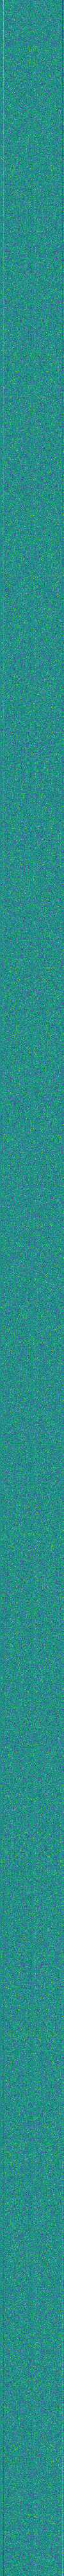
\includegraphics[interpolate=false,width=1.000000in,height=1.000000in]{antiderivative_ci_10-img0.png}}%
\end{pgfscope}%
\begin{pgfscope}%
\pgfsetbuttcap%
\pgfsetroundjoin%
\definecolor{currentfill}{rgb}{0.000000,0.000000,0.000000}%
\pgfsetfillcolor{currentfill}%
\pgfsetlinewidth{0.803000pt}%
\definecolor{currentstroke}{rgb}{0.000000,0.000000,0.000000}%
\pgfsetstrokecolor{currentstroke}%
\pgfsetdash{}{0pt}%
\pgfsys@defobject{currentmarker}{\pgfqpoint{0.000000in}{-0.048611in}}{\pgfqpoint{0.000000in}{0.000000in}}{%
\pgfpathmoveto{\pgfqpoint{0.000000in}{0.000000in}}%
\pgfpathlineto{\pgfqpoint{0.000000in}{-0.048611in}}%
\pgfusepath{stroke,fill}%
}%
\begin{pgfscope}%
\pgfsys@transformshift{0.800000in}{0.528000in}%
\pgfsys@useobject{currentmarker}{}%
\end{pgfscope}%
\end{pgfscope}%
\begin{pgfscope}%
\definecolor{textcolor}{rgb}{0.000000,0.000000,0.000000}%
\pgfsetstrokecolor{textcolor}%
\pgfsetfillcolor{textcolor}%
\pgftext[x=0.800000in,y=0.430778in,,top]{\color{textcolor}{\rmfamily\fontsize{12.000000}{14.400000}\selectfont\catcode`\^=\active\def^{\ifmmode\sp\else\^{}\fi}\catcode`\%=\active\def%{\%}0}}%
\end{pgfscope}%
\begin{pgfscope}%
\pgfsetbuttcap%
\pgfsetroundjoin%
\definecolor{currentfill}{rgb}{0.000000,0.000000,0.000000}%
\pgfsetfillcolor{currentfill}%
\pgfsetlinewidth{0.803000pt}%
\definecolor{currentstroke}{rgb}{0.000000,0.000000,0.000000}%
\pgfsetstrokecolor{currentstroke}%
\pgfsetdash{}{0pt}%
\pgfsys@defobject{currentmarker}{\pgfqpoint{0.000000in}{-0.048611in}}{\pgfqpoint{0.000000in}{0.000000in}}{%
\pgfpathmoveto{\pgfqpoint{0.000000in}{0.000000in}}%
\pgfpathlineto{\pgfqpoint{0.000000in}{-0.048611in}}%
\pgfusepath{stroke,fill}%
}%
\begin{pgfscope}%
\pgfsys@transformshift{1.593600in}{0.528000in}%
\pgfsys@useobject{currentmarker}{}%
\end{pgfscope}%
\end{pgfscope}%
\begin{pgfscope}%
\definecolor{textcolor}{rgb}{0.000000,0.000000,0.000000}%
\pgfsetstrokecolor{textcolor}%
\pgfsetfillcolor{textcolor}%
\pgftext[x=1.593600in,y=0.430778in,,top]{\color{textcolor}{\rmfamily\fontsize{12.000000}{14.400000}\selectfont\catcode`\^=\active\def^{\ifmmode\sp\else\^{}\fi}\catcode`\%=\active\def%{\%}10}}%
\end{pgfscope}%
\begin{pgfscope}%
\pgfsetbuttcap%
\pgfsetroundjoin%
\definecolor{currentfill}{rgb}{0.000000,0.000000,0.000000}%
\pgfsetfillcolor{currentfill}%
\pgfsetlinewidth{0.803000pt}%
\definecolor{currentstroke}{rgb}{0.000000,0.000000,0.000000}%
\pgfsetstrokecolor{currentstroke}%
\pgfsetdash{}{0pt}%
\pgfsys@defobject{currentmarker}{\pgfqpoint{0.000000in}{-0.048611in}}{\pgfqpoint{0.000000in}{0.000000in}}{%
\pgfpathmoveto{\pgfqpoint{0.000000in}{0.000000in}}%
\pgfpathlineto{\pgfqpoint{0.000000in}{-0.048611in}}%
\pgfusepath{stroke,fill}%
}%
\begin{pgfscope}%
\pgfsys@transformshift{2.387200in}{0.528000in}%
\pgfsys@useobject{currentmarker}{}%
\end{pgfscope}%
\end{pgfscope}%
\begin{pgfscope}%
\definecolor{textcolor}{rgb}{0.000000,0.000000,0.000000}%
\pgfsetstrokecolor{textcolor}%
\pgfsetfillcolor{textcolor}%
\pgftext[x=2.387200in,y=0.430778in,,top]{\color{textcolor}{\rmfamily\fontsize{12.000000}{14.400000}\selectfont\catcode`\^=\active\def^{\ifmmode\sp\else\^{}\fi}\catcode`\%=\active\def%{\%}20}}%
\end{pgfscope}%
\begin{pgfscope}%
\pgfsetbuttcap%
\pgfsetroundjoin%
\definecolor{currentfill}{rgb}{0.000000,0.000000,0.000000}%
\pgfsetfillcolor{currentfill}%
\pgfsetlinewidth{0.803000pt}%
\definecolor{currentstroke}{rgb}{0.000000,0.000000,0.000000}%
\pgfsetstrokecolor{currentstroke}%
\pgfsetdash{}{0pt}%
\pgfsys@defobject{currentmarker}{\pgfqpoint{0.000000in}{-0.048611in}}{\pgfqpoint{0.000000in}{0.000000in}}{%
\pgfpathmoveto{\pgfqpoint{0.000000in}{0.000000in}}%
\pgfpathlineto{\pgfqpoint{0.000000in}{-0.048611in}}%
\pgfusepath{stroke,fill}%
}%
\begin{pgfscope}%
\pgfsys@transformshift{3.180800in}{0.528000in}%
\pgfsys@useobject{currentmarker}{}%
\end{pgfscope}%
\end{pgfscope}%
\begin{pgfscope}%
\definecolor{textcolor}{rgb}{0.000000,0.000000,0.000000}%
\pgfsetstrokecolor{textcolor}%
\pgfsetfillcolor{textcolor}%
\pgftext[x=3.180800in,y=0.430778in,,top]{\color{textcolor}{\rmfamily\fontsize{12.000000}{14.400000}\selectfont\catcode`\^=\active\def^{\ifmmode\sp\else\^{}\fi}\catcode`\%=\active\def%{\%}30}}%
\end{pgfscope}%
\begin{pgfscope}%
\pgfsetbuttcap%
\pgfsetroundjoin%
\definecolor{currentfill}{rgb}{0.000000,0.000000,0.000000}%
\pgfsetfillcolor{currentfill}%
\pgfsetlinewidth{0.803000pt}%
\definecolor{currentstroke}{rgb}{0.000000,0.000000,0.000000}%
\pgfsetstrokecolor{currentstroke}%
\pgfsetdash{}{0pt}%
\pgfsys@defobject{currentmarker}{\pgfqpoint{0.000000in}{-0.048611in}}{\pgfqpoint{0.000000in}{0.000000in}}{%
\pgfpathmoveto{\pgfqpoint{0.000000in}{0.000000in}}%
\pgfpathlineto{\pgfqpoint{0.000000in}{-0.048611in}}%
\pgfusepath{stroke,fill}%
}%
\begin{pgfscope}%
\pgfsys@transformshift{3.974400in}{0.528000in}%
\pgfsys@useobject{currentmarker}{}%
\end{pgfscope}%
\end{pgfscope}%
\begin{pgfscope}%
\definecolor{textcolor}{rgb}{0.000000,0.000000,0.000000}%
\pgfsetstrokecolor{textcolor}%
\pgfsetfillcolor{textcolor}%
\pgftext[x=3.974400in,y=0.430778in,,top]{\color{textcolor}{\rmfamily\fontsize{12.000000}{14.400000}\selectfont\catcode`\^=\active\def^{\ifmmode\sp\else\^{}\fi}\catcode`\%=\active\def%{\%}40}}%
\end{pgfscope}%
\begin{pgfscope}%
\pgfsetbuttcap%
\pgfsetroundjoin%
\definecolor{currentfill}{rgb}{0.000000,0.000000,0.000000}%
\pgfsetfillcolor{currentfill}%
\pgfsetlinewidth{0.803000pt}%
\definecolor{currentstroke}{rgb}{0.000000,0.000000,0.000000}%
\pgfsetstrokecolor{currentstroke}%
\pgfsetdash{}{0pt}%
\pgfsys@defobject{currentmarker}{\pgfqpoint{0.000000in}{-0.048611in}}{\pgfqpoint{0.000000in}{0.000000in}}{%
\pgfpathmoveto{\pgfqpoint{0.000000in}{0.000000in}}%
\pgfpathlineto{\pgfqpoint{0.000000in}{-0.048611in}}%
\pgfusepath{stroke,fill}%
}%
\begin{pgfscope}%
\pgfsys@transformshift{4.768000in}{0.528000in}%
\pgfsys@useobject{currentmarker}{}%
\end{pgfscope}%
\end{pgfscope}%
\begin{pgfscope}%
\definecolor{textcolor}{rgb}{0.000000,0.000000,0.000000}%
\pgfsetstrokecolor{textcolor}%
\pgfsetfillcolor{textcolor}%
\pgftext[x=4.768000in,y=0.430778in,,top]{\color{textcolor}{\rmfamily\fontsize{12.000000}{14.400000}\selectfont\catcode`\^=\active\def^{\ifmmode\sp\else\^{}\fi}\catcode`\%=\active\def%{\%}50}}%
\end{pgfscope}%
\begin{pgfscope}%
\definecolor{textcolor}{rgb}{0.000000,0.000000,0.000000}%
\pgfsetstrokecolor{textcolor}%
\pgfsetfillcolor{textcolor}%
\pgftext[x=2.784000in,y=0.213927in,,top]{\color{textcolor}{\rmfamily\fontsize{12.000000}{14.400000}\selectfont\catcode`\^=\active\def^{\ifmmode\sp\else\^{}\fi}\catcode`\%=\active\def%{\%}input coefficients}}%
\end{pgfscope}%
\begin{pgfscope}%
\pgfsetbuttcap%
\pgfsetroundjoin%
\definecolor{currentfill}{rgb}{0.000000,0.000000,0.000000}%
\pgfsetfillcolor{currentfill}%
\pgfsetlinewidth{0.803000pt}%
\definecolor{currentstroke}{rgb}{0.000000,0.000000,0.000000}%
\pgfsetstrokecolor{currentstroke}%
\pgfsetdash{}{0pt}%
\pgfsys@defobject{currentmarker}{\pgfqpoint{-0.048611in}{0.000000in}}{\pgfqpoint{-0.000000in}{0.000000in}}{%
\pgfpathmoveto{\pgfqpoint{-0.000000in}{0.000000in}}%
\pgfpathlineto{\pgfqpoint{-0.048611in}{0.000000in}}%
\pgfusepath{stroke,fill}%
}%
\begin{pgfscope}%
\pgfsys@transformshift{0.800000in}{4.224000in}%
\pgfsys@useobject{currentmarker}{}%
\end{pgfscope}%
\end{pgfscope}%
\begin{pgfscope}%
\definecolor{textcolor}{rgb}{0.000000,0.000000,0.000000}%
\pgfsetstrokecolor{textcolor}%
\pgfsetfillcolor{textcolor}%
\pgftext[x=0.596739in, y=4.160686in, left, base]{\color{textcolor}{\rmfamily\fontsize{12.000000}{14.400000}\selectfont\catcode`\^=\active\def^{\ifmmode\sp\else\^{}\fi}\catcode`\%=\active\def%{\%}0}}%
\end{pgfscope}%
\begin{pgfscope}%
\pgfsetbuttcap%
\pgfsetroundjoin%
\definecolor{currentfill}{rgb}{0.000000,0.000000,0.000000}%
\pgfsetfillcolor{currentfill}%
\pgfsetlinewidth{0.803000pt}%
\definecolor{currentstroke}{rgb}{0.000000,0.000000,0.000000}%
\pgfsetstrokecolor{currentstroke}%
\pgfsetdash{}{0pt}%
\pgfsys@defobject{currentmarker}{\pgfqpoint{-0.048611in}{0.000000in}}{\pgfqpoint{-0.000000in}{0.000000in}}{%
\pgfpathmoveto{\pgfqpoint{-0.000000in}{0.000000in}}%
\pgfpathlineto{\pgfqpoint{-0.048611in}{0.000000in}}%
\pgfusepath{stroke,fill}%
}%
\begin{pgfscope}%
\pgfsys@transformshift{0.800000in}{3.762000in}%
\pgfsys@useobject{currentmarker}{}%
\end{pgfscope}%
\end{pgfscope}%
\begin{pgfscope}%
\definecolor{textcolor}{rgb}{0.000000,0.000000,0.000000}%
\pgfsetstrokecolor{textcolor}%
\pgfsetfillcolor{textcolor}%
\pgftext[x=0.384662in, y=3.698686in, left, base]{\color{textcolor}{\rmfamily\fontsize{12.000000}{14.400000}\selectfont\catcode`\^=\active\def^{\ifmmode\sp\else\^{}\fi}\catcode`\%=\active\def%{\%}500}}%
\end{pgfscope}%
\begin{pgfscope}%
\pgfsetbuttcap%
\pgfsetroundjoin%
\definecolor{currentfill}{rgb}{0.000000,0.000000,0.000000}%
\pgfsetfillcolor{currentfill}%
\pgfsetlinewidth{0.803000pt}%
\definecolor{currentstroke}{rgb}{0.000000,0.000000,0.000000}%
\pgfsetstrokecolor{currentstroke}%
\pgfsetdash{}{0pt}%
\pgfsys@defobject{currentmarker}{\pgfqpoint{-0.048611in}{0.000000in}}{\pgfqpoint{-0.000000in}{0.000000in}}{%
\pgfpathmoveto{\pgfqpoint{-0.000000in}{0.000000in}}%
\pgfpathlineto{\pgfqpoint{-0.048611in}{0.000000in}}%
\pgfusepath{stroke,fill}%
}%
\begin{pgfscope}%
\pgfsys@transformshift{0.800000in}{3.300000in}%
\pgfsys@useobject{currentmarker}{}%
\end{pgfscope}%
\end{pgfscope}%
\begin{pgfscope}%
\definecolor{textcolor}{rgb}{0.000000,0.000000,0.000000}%
\pgfsetstrokecolor{textcolor}%
\pgfsetfillcolor{textcolor}%
\pgftext[x=0.278624in, y=3.236686in, left, base]{\color{textcolor}{\rmfamily\fontsize{12.000000}{14.400000}\selectfont\catcode`\^=\active\def^{\ifmmode\sp\else\^{}\fi}\catcode`\%=\active\def%{\%}1000}}%
\end{pgfscope}%
\begin{pgfscope}%
\pgfsetbuttcap%
\pgfsetroundjoin%
\definecolor{currentfill}{rgb}{0.000000,0.000000,0.000000}%
\pgfsetfillcolor{currentfill}%
\pgfsetlinewidth{0.803000pt}%
\definecolor{currentstroke}{rgb}{0.000000,0.000000,0.000000}%
\pgfsetstrokecolor{currentstroke}%
\pgfsetdash{}{0pt}%
\pgfsys@defobject{currentmarker}{\pgfqpoint{-0.048611in}{0.000000in}}{\pgfqpoint{-0.000000in}{0.000000in}}{%
\pgfpathmoveto{\pgfqpoint{-0.000000in}{0.000000in}}%
\pgfpathlineto{\pgfqpoint{-0.048611in}{0.000000in}}%
\pgfusepath{stroke,fill}%
}%
\begin{pgfscope}%
\pgfsys@transformshift{0.800000in}{2.838000in}%
\pgfsys@useobject{currentmarker}{}%
\end{pgfscope}%
\end{pgfscope}%
\begin{pgfscope}%
\definecolor{textcolor}{rgb}{0.000000,0.000000,0.000000}%
\pgfsetstrokecolor{textcolor}%
\pgfsetfillcolor{textcolor}%
\pgftext[x=0.278624in, y=2.774686in, left, base]{\color{textcolor}{\rmfamily\fontsize{12.000000}{14.400000}\selectfont\catcode`\^=\active\def^{\ifmmode\sp\else\^{}\fi}\catcode`\%=\active\def%{\%}1500}}%
\end{pgfscope}%
\begin{pgfscope}%
\pgfsetbuttcap%
\pgfsetroundjoin%
\definecolor{currentfill}{rgb}{0.000000,0.000000,0.000000}%
\pgfsetfillcolor{currentfill}%
\pgfsetlinewidth{0.803000pt}%
\definecolor{currentstroke}{rgb}{0.000000,0.000000,0.000000}%
\pgfsetstrokecolor{currentstroke}%
\pgfsetdash{}{0pt}%
\pgfsys@defobject{currentmarker}{\pgfqpoint{-0.048611in}{0.000000in}}{\pgfqpoint{-0.000000in}{0.000000in}}{%
\pgfpathmoveto{\pgfqpoint{-0.000000in}{0.000000in}}%
\pgfpathlineto{\pgfqpoint{-0.048611in}{0.000000in}}%
\pgfusepath{stroke,fill}%
}%
\begin{pgfscope}%
\pgfsys@transformshift{0.800000in}{2.376000in}%
\pgfsys@useobject{currentmarker}{}%
\end{pgfscope}%
\end{pgfscope}%
\begin{pgfscope}%
\definecolor{textcolor}{rgb}{0.000000,0.000000,0.000000}%
\pgfsetstrokecolor{textcolor}%
\pgfsetfillcolor{textcolor}%
\pgftext[x=0.278624in, y=2.312686in, left, base]{\color{textcolor}{\rmfamily\fontsize{12.000000}{14.400000}\selectfont\catcode`\^=\active\def^{\ifmmode\sp\else\^{}\fi}\catcode`\%=\active\def%{\%}2000}}%
\end{pgfscope}%
\begin{pgfscope}%
\pgfsetbuttcap%
\pgfsetroundjoin%
\definecolor{currentfill}{rgb}{0.000000,0.000000,0.000000}%
\pgfsetfillcolor{currentfill}%
\pgfsetlinewidth{0.803000pt}%
\definecolor{currentstroke}{rgb}{0.000000,0.000000,0.000000}%
\pgfsetstrokecolor{currentstroke}%
\pgfsetdash{}{0pt}%
\pgfsys@defobject{currentmarker}{\pgfqpoint{-0.048611in}{0.000000in}}{\pgfqpoint{-0.000000in}{0.000000in}}{%
\pgfpathmoveto{\pgfqpoint{-0.000000in}{0.000000in}}%
\pgfpathlineto{\pgfqpoint{-0.048611in}{0.000000in}}%
\pgfusepath{stroke,fill}%
}%
\begin{pgfscope}%
\pgfsys@transformshift{0.800000in}{1.914000in}%
\pgfsys@useobject{currentmarker}{}%
\end{pgfscope}%
\end{pgfscope}%
\begin{pgfscope}%
\definecolor{textcolor}{rgb}{0.000000,0.000000,0.000000}%
\pgfsetstrokecolor{textcolor}%
\pgfsetfillcolor{textcolor}%
\pgftext[x=0.278624in, y=1.850686in, left, base]{\color{textcolor}{\rmfamily\fontsize{12.000000}{14.400000}\selectfont\catcode`\^=\active\def^{\ifmmode\sp\else\^{}\fi}\catcode`\%=\active\def%{\%}2500}}%
\end{pgfscope}%
\begin{pgfscope}%
\pgfsetbuttcap%
\pgfsetroundjoin%
\definecolor{currentfill}{rgb}{0.000000,0.000000,0.000000}%
\pgfsetfillcolor{currentfill}%
\pgfsetlinewidth{0.803000pt}%
\definecolor{currentstroke}{rgb}{0.000000,0.000000,0.000000}%
\pgfsetstrokecolor{currentstroke}%
\pgfsetdash{}{0pt}%
\pgfsys@defobject{currentmarker}{\pgfqpoint{-0.048611in}{0.000000in}}{\pgfqpoint{-0.000000in}{0.000000in}}{%
\pgfpathmoveto{\pgfqpoint{-0.000000in}{0.000000in}}%
\pgfpathlineto{\pgfqpoint{-0.048611in}{0.000000in}}%
\pgfusepath{stroke,fill}%
}%
\begin{pgfscope}%
\pgfsys@transformshift{0.800000in}{1.452000in}%
\pgfsys@useobject{currentmarker}{}%
\end{pgfscope}%
\end{pgfscope}%
\begin{pgfscope}%
\definecolor{textcolor}{rgb}{0.000000,0.000000,0.000000}%
\pgfsetstrokecolor{textcolor}%
\pgfsetfillcolor{textcolor}%
\pgftext[x=0.278624in, y=1.388686in, left, base]{\color{textcolor}{\rmfamily\fontsize{12.000000}{14.400000}\selectfont\catcode`\^=\active\def^{\ifmmode\sp\else\^{}\fi}\catcode`\%=\active\def%{\%}3000}}%
\end{pgfscope}%
\begin{pgfscope}%
\pgfsetbuttcap%
\pgfsetroundjoin%
\definecolor{currentfill}{rgb}{0.000000,0.000000,0.000000}%
\pgfsetfillcolor{currentfill}%
\pgfsetlinewidth{0.803000pt}%
\definecolor{currentstroke}{rgb}{0.000000,0.000000,0.000000}%
\pgfsetstrokecolor{currentstroke}%
\pgfsetdash{}{0pt}%
\pgfsys@defobject{currentmarker}{\pgfqpoint{-0.048611in}{0.000000in}}{\pgfqpoint{-0.000000in}{0.000000in}}{%
\pgfpathmoveto{\pgfqpoint{-0.000000in}{0.000000in}}%
\pgfpathlineto{\pgfqpoint{-0.048611in}{0.000000in}}%
\pgfusepath{stroke,fill}%
}%
\begin{pgfscope}%
\pgfsys@transformshift{0.800000in}{0.990000in}%
\pgfsys@useobject{currentmarker}{}%
\end{pgfscope}%
\end{pgfscope}%
\begin{pgfscope}%
\definecolor{textcolor}{rgb}{0.000000,0.000000,0.000000}%
\pgfsetstrokecolor{textcolor}%
\pgfsetfillcolor{textcolor}%
\pgftext[x=0.278624in, y=0.926686in, left, base]{\color{textcolor}{\rmfamily\fontsize{12.000000}{14.400000}\selectfont\catcode`\^=\active\def^{\ifmmode\sp\else\^{}\fi}\catcode`\%=\active\def%{\%}3500}}%
\end{pgfscope}%
\begin{pgfscope}%
\pgfsetbuttcap%
\pgfsetroundjoin%
\definecolor{currentfill}{rgb}{0.000000,0.000000,0.000000}%
\pgfsetfillcolor{currentfill}%
\pgfsetlinewidth{0.803000pt}%
\definecolor{currentstroke}{rgb}{0.000000,0.000000,0.000000}%
\pgfsetstrokecolor{currentstroke}%
\pgfsetdash{}{0pt}%
\pgfsys@defobject{currentmarker}{\pgfqpoint{-0.048611in}{0.000000in}}{\pgfqpoint{-0.000000in}{0.000000in}}{%
\pgfpathmoveto{\pgfqpoint{-0.000000in}{0.000000in}}%
\pgfpathlineto{\pgfqpoint{-0.048611in}{0.000000in}}%
\pgfusepath{stroke,fill}%
}%
\begin{pgfscope}%
\pgfsys@transformshift{0.800000in}{0.528000in}%
\pgfsys@useobject{currentmarker}{}%
\end{pgfscope}%
\end{pgfscope}%
\begin{pgfscope}%
\definecolor{textcolor}{rgb}{0.000000,0.000000,0.000000}%
\pgfsetstrokecolor{textcolor}%
\pgfsetfillcolor{textcolor}%
\pgftext[x=0.278624in, y=0.464686in, left, base]{\color{textcolor}{\rmfamily\fontsize{12.000000}{14.400000}\selectfont\catcode`\^=\active\def^{\ifmmode\sp\else\^{}\fi}\catcode`\%=\active\def%{\%}4000}}%
\end{pgfscope}%
\begin{pgfscope}%
\definecolor{textcolor}{rgb}{0.000000,0.000000,0.000000}%
\pgfsetstrokecolor{textcolor}%
\pgfsetfillcolor{textcolor}%
\pgftext[x=0.223069in,y=2.376000in,,bottom,rotate=90.000000]{\color{textcolor}{\rmfamily\fontsize{12.000000}{14.400000}\selectfont\catcode`\^=\active\def^{\ifmmode\sp\else\^{}\fi}\catcode`\%=\active\def%{\%}samples}}%
\end{pgfscope}%
\begin{pgfscope}%
\pgfsetrectcap%
\pgfsetmiterjoin%
\pgfsetlinewidth{0.803000pt}%
\definecolor{currentstroke}{rgb}{0.000000,0.000000,0.000000}%
\pgfsetstrokecolor{currentstroke}%
\pgfsetdash{}{0pt}%
\pgfpathmoveto{\pgfqpoint{0.800000in}{0.528000in}}%
\pgfpathlineto{\pgfqpoint{0.800000in}{4.224000in}}%
\pgfusepath{stroke}%
\end{pgfscope}%
\begin{pgfscope}%
\pgfsetrectcap%
\pgfsetmiterjoin%
\pgfsetlinewidth{0.803000pt}%
\definecolor{currentstroke}{rgb}{0.000000,0.000000,0.000000}%
\pgfsetstrokecolor{currentstroke}%
\pgfsetdash{}{0pt}%
\pgfpathmoveto{\pgfqpoint{4.768000in}{0.528000in}}%
\pgfpathlineto{\pgfqpoint{4.768000in}{4.224000in}}%
\pgfusepath{stroke}%
\end{pgfscope}%
\begin{pgfscope}%
\pgfsetrectcap%
\pgfsetmiterjoin%
\pgfsetlinewidth{0.803000pt}%
\definecolor{currentstroke}{rgb}{0.000000,0.000000,0.000000}%
\pgfsetstrokecolor{currentstroke}%
\pgfsetdash{}{0pt}%
\pgfpathmoveto{\pgfqpoint{0.800000in}{0.528000in}}%
\pgfpathlineto{\pgfqpoint{4.768000in}{0.528000in}}%
\pgfusepath{stroke}%
\end{pgfscope}%
\begin{pgfscope}%
\pgfsetrectcap%
\pgfsetmiterjoin%
\pgfsetlinewidth{0.803000pt}%
\definecolor{currentstroke}{rgb}{0.000000,0.000000,0.000000}%
\pgfsetstrokecolor{currentstroke}%
\pgfsetdash{}{0pt}%
\pgfpathmoveto{\pgfqpoint{0.800000in}{4.224000in}}%
\pgfpathlineto{\pgfqpoint{4.768000in}{4.224000in}}%
\pgfusepath{stroke}%
\end{pgfscope}%
\begin{pgfscope}%
\pgfsetbuttcap%
\pgfsetmiterjoin%
\pgfsetlinewidth{0.000000pt}%
\definecolor{currentstroke}{rgb}{0.000000,0.000000,0.000000}%
\pgfsetstrokecolor{currentstroke}%
\pgfsetstrokeopacity{0.000000}%
\pgfsetdash{}{0pt}%
\pgfpathmoveto{\pgfqpoint{5.016000in}{0.528000in}}%
\pgfpathlineto{\pgfqpoint{5.200800in}{0.528000in}}%
\pgfpathlineto{\pgfqpoint{5.200800in}{4.224000in}}%
\pgfpathlineto{\pgfqpoint{5.016000in}{4.224000in}}%
\pgfpathlineto{\pgfqpoint{5.016000in}{0.528000in}}%
\pgfpathclose%
\pgfusepath{}%
\end{pgfscope}%
\begin{pgfscope}%
\pgfsys@transformshift{5.020000in}{0.530000in}%
\pgftext[left,bottom]{
\includegraphics[interpolate=true,width=0.180000in,height=3.690000in]{antiderivative_ci_10-img1.png}}%
\end{pgfscope}%
\begin{pgfscope}%
\pgfsetbuttcap%
\pgfsetroundjoin%
\definecolor{currentfill}{rgb}{0.000000,0.000000,0.000000}%
\pgfsetfillcolor{currentfill}%
\pgfsetlinewidth{0.803000pt}%
\definecolor{currentstroke}{rgb}{0.000000,0.000000,0.000000}%
\pgfsetstrokecolor{currentstroke}%
\pgfsetdash{}{0pt}%
\pgfsys@defobject{currentmarker}{\pgfqpoint{0.000000in}{0.000000in}}{\pgfqpoint{0.048611in}{0.000000in}}{%
\pgfpathmoveto{\pgfqpoint{0.000000in}{0.000000in}}%
\pgfpathlineto{\pgfqpoint{0.048611in}{0.000000in}}%
\pgfusepath{stroke,fill}%
}%
\begin{pgfscope}%
\pgfsys@transformshift{5.200800in}{0.547966in}%
\pgfsys@useobject{currentmarker}{}%
\end{pgfscope}%
\end{pgfscope}%
\begin{pgfscope}%
\definecolor{textcolor}{rgb}{0.000000,0.000000,0.000000}%
\pgfsetstrokecolor{textcolor}%
\pgfsetfillcolor{textcolor}%
\pgftext[x=5.298022in, y=0.484652in, left, base]{\color{textcolor}{\rmfamily\fontsize{12.000000}{14.400000}\selectfont\catcode`\^=\active\def^{\ifmmode\sp\else\^{}\fi}\catcode`\%=\active\def%{\%}\ensuremath{-}100}}%
\end{pgfscope}%
\begin{pgfscope}%
\pgfsetbuttcap%
\pgfsetroundjoin%
\definecolor{currentfill}{rgb}{0.000000,0.000000,0.000000}%
\pgfsetfillcolor{currentfill}%
\pgfsetlinewidth{0.803000pt}%
\definecolor{currentstroke}{rgb}{0.000000,0.000000,0.000000}%
\pgfsetstrokecolor{currentstroke}%
\pgfsetdash{}{0pt}%
\pgfsys@defobject{currentmarker}{\pgfqpoint{0.000000in}{0.000000in}}{\pgfqpoint{0.048611in}{0.000000in}}{%
\pgfpathmoveto{\pgfqpoint{0.000000in}{0.000000in}}%
\pgfpathlineto{\pgfqpoint{0.048611in}{0.000000in}}%
\pgfusepath{stroke,fill}%
}%
\begin{pgfscope}%
\pgfsys@transformshift{5.200800in}{0.998231in}%
\pgfsys@useobject{currentmarker}{}%
\end{pgfscope}%
\end{pgfscope}%
\begin{pgfscope}%
\definecolor{textcolor}{rgb}{0.000000,0.000000,0.000000}%
\pgfsetstrokecolor{textcolor}%
\pgfsetfillcolor{textcolor}%
\pgftext[x=5.298022in, y=0.934917in, left, base]{\color{textcolor}{\rmfamily\fontsize{12.000000}{14.400000}\selectfont\catcode`\^=\active\def^{\ifmmode\sp\else\^{}\fi}\catcode`\%=\active\def%{\%}\ensuremath{-}75}}%
\end{pgfscope}%
\begin{pgfscope}%
\pgfsetbuttcap%
\pgfsetroundjoin%
\definecolor{currentfill}{rgb}{0.000000,0.000000,0.000000}%
\pgfsetfillcolor{currentfill}%
\pgfsetlinewidth{0.803000pt}%
\definecolor{currentstroke}{rgb}{0.000000,0.000000,0.000000}%
\pgfsetstrokecolor{currentstroke}%
\pgfsetdash{}{0pt}%
\pgfsys@defobject{currentmarker}{\pgfqpoint{0.000000in}{0.000000in}}{\pgfqpoint{0.048611in}{0.000000in}}{%
\pgfpathmoveto{\pgfqpoint{0.000000in}{0.000000in}}%
\pgfpathlineto{\pgfqpoint{0.048611in}{0.000000in}}%
\pgfusepath{stroke,fill}%
}%
\begin{pgfscope}%
\pgfsys@transformshift{5.200800in}{1.448497in}%
\pgfsys@useobject{currentmarker}{}%
\end{pgfscope}%
\end{pgfscope}%
\begin{pgfscope}%
\definecolor{textcolor}{rgb}{0.000000,0.000000,0.000000}%
\pgfsetstrokecolor{textcolor}%
\pgfsetfillcolor{textcolor}%
\pgftext[x=5.298022in, y=1.385183in, left, base]{\color{textcolor}{\rmfamily\fontsize{12.000000}{14.400000}\selectfont\catcode`\^=\active\def^{\ifmmode\sp\else\^{}\fi}\catcode`\%=\active\def%{\%}\ensuremath{-}50}}%
\end{pgfscope}%
\begin{pgfscope}%
\pgfsetbuttcap%
\pgfsetroundjoin%
\definecolor{currentfill}{rgb}{0.000000,0.000000,0.000000}%
\pgfsetfillcolor{currentfill}%
\pgfsetlinewidth{0.803000pt}%
\definecolor{currentstroke}{rgb}{0.000000,0.000000,0.000000}%
\pgfsetstrokecolor{currentstroke}%
\pgfsetdash{}{0pt}%
\pgfsys@defobject{currentmarker}{\pgfqpoint{0.000000in}{0.000000in}}{\pgfqpoint{0.048611in}{0.000000in}}{%
\pgfpathmoveto{\pgfqpoint{0.000000in}{0.000000in}}%
\pgfpathlineto{\pgfqpoint{0.048611in}{0.000000in}}%
\pgfusepath{stroke,fill}%
}%
\begin{pgfscope}%
\pgfsys@transformshift{5.200800in}{1.898762in}%
\pgfsys@useobject{currentmarker}{}%
\end{pgfscope}%
\end{pgfscope}%
\begin{pgfscope}%
\definecolor{textcolor}{rgb}{0.000000,0.000000,0.000000}%
\pgfsetstrokecolor{textcolor}%
\pgfsetfillcolor{textcolor}%
\pgftext[x=5.298022in, y=1.835448in, left, base]{\color{textcolor}{\rmfamily\fontsize{12.000000}{14.400000}\selectfont\catcode`\^=\active\def^{\ifmmode\sp\else\^{}\fi}\catcode`\%=\active\def%{\%}\ensuremath{-}25}}%
\end{pgfscope}%
\begin{pgfscope}%
\pgfsetbuttcap%
\pgfsetroundjoin%
\definecolor{currentfill}{rgb}{0.000000,0.000000,0.000000}%
\pgfsetfillcolor{currentfill}%
\pgfsetlinewidth{0.803000pt}%
\definecolor{currentstroke}{rgb}{0.000000,0.000000,0.000000}%
\pgfsetstrokecolor{currentstroke}%
\pgfsetdash{}{0pt}%
\pgfsys@defobject{currentmarker}{\pgfqpoint{0.000000in}{0.000000in}}{\pgfqpoint{0.048611in}{0.000000in}}{%
\pgfpathmoveto{\pgfqpoint{0.000000in}{0.000000in}}%
\pgfpathlineto{\pgfqpoint{0.048611in}{0.000000in}}%
\pgfusepath{stroke,fill}%
}%
\begin{pgfscope}%
\pgfsys@transformshift{5.200800in}{2.349028in}%
\pgfsys@useobject{currentmarker}{}%
\end{pgfscope}%
\end{pgfscope}%
\begin{pgfscope}%
\definecolor{textcolor}{rgb}{0.000000,0.000000,0.000000}%
\pgfsetstrokecolor{textcolor}%
\pgfsetfillcolor{textcolor}%
\pgftext[x=5.298022in, y=2.285714in, left, base]{\color{textcolor}{\rmfamily\fontsize{12.000000}{14.400000}\selectfont\catcode`\^=\active\def^{\ifmmode\sp\else\^{}\fi}\catcode`\%=\active\def%{\%}0}}%
\end{pgfscope}%
\begin{pgfscope}%
\pgfsetbuttcap%
\pgfsetroundjoin%
\definecolor{currentfill}{rgb}{0.000000,0.000000,0.000000}%
\pgfsetfillcolor{currentfill}%
\pgfsetlinewidth{0.803000pt}%
\definecolor{currentstroke}{rgb}{0.000000,0.000000,0.000000}%
\pgfsetstrokecolor{currentstroke}%
\pgfsetdash{}{0pt}%
\pgfsys@defobject{currentmarker}{\pgfqpoint{0.000000in}{0.000000in}}{\pgfqpoint{0.048611in}{0.000000in}}{%
\pgfpathmoveto{\pgfqpoint{0.000000in}{0.000000in}}%
\pgfpathlineto{\pgfqpoint{0.048611in}{0.000000in}}%
\pgfusepath{stroke,fill}%
}%
\begin{pgfscope}%
\pgfsys@transformshift{5.200800in}{2.799293in}%
\pgfsys@useobject{currentmarker}{}%
\end{pgfscope}%
\end{pgfscope}%
\begin{pgfscope}%
\definecolor{textcolor}{rgb}{0.000000,0.000000,0.000000}%
\pgfsetstrokecolor{textcolor}%
\pgfsetfillcolor{textcolor}%
\pgftext[x=5.298022in, y=2.735979in, left, base]{\color{textcolor}{\rmfamily\fontsize{12.000000}{14.400000}\selectfont\catcode`\^=\active\def^{\ifmmode\sp\else\^{}\fi}\catcode`\%=\active\def%{\%}25}}%
\end{pgfscope}%
\begin{pgfscope}%
\pgfsetbuttcap%
\pgfsetroundjoin%
\definecolor{currentfill}{rgb}{0.000000,0.000000,0.000000}%
\pgfsetfillcolor{currentfill}%
\pgfsetlinewidth{0.803000pt}%
\definecolor{currentstroke}{rgb}{0.000000,0.000000,0.000000}%
\pgfsetstrokecolor{currentstroke}%
\pgfsetdash{}{0pt}%
\pgfsys@defobject{currentmarker}{\pgfqpoint{0.000000in}{0.000000in}}{\pgfqpoint{0.048611in}{0.000000in}}{%
\pgfpathmoveto{\pgfqpoint{0.000000in}{0.000000in}}%
\pgfpathlineto{\pgfqpoint{0.048611in}{0.000000in}}%
\pgfusepath{stroke,fill}%
}%
\begin{pgfscope}%
\pgfsys@transformshift{5.200800in}{3.249559in}%
\pgfsys@useobject{currentmarker}{}%
\end{pgfscope}%
\end{pgfscope}%
\begin{pgfscope}%
\definecolor{textcolor}{rgb}{0.000000,0.000000,0.000000}%
\pgfsetstrokecolor{textcolor}%
\pgfsetfillcolor{textcolor}%
\pgftext[x=5.298022in, y=3.186245in, left, base]{\color{textcolor}{\rmfamily\fontsize{12.000000}{14.400000}\selectfont\catcode`\^=\active\def^{\ifmmode\sp\else\^{}\fi}\catcode`\%=\active\def%{\%}50}}%
\end{pgfscope}%
\begin{pgfscope}%
\pgfsetbuttcap%
\pgfsetroundjoin%
\definecolor{currentfill}{rgb}{0.000000,0.000000,0.000000}%
\pgfsetfillcolor{currentfill}%
\pgfsetlinewidth{0.803000pt}%
\definecolor{currentstroke}{rgb}{0.000000,0.000000,0.000000}%
\pgfsetstrokecolor{currentstroke}%
\pgfsetdash{}{0pt}%
\pgfsys@defobject{currentmarker}{\pgfqpoint{0.000000in}{0.000000in}}{\pgfqpoint{0.048611in}{0.000000in}}{%
\pgfpathmoveto{\pgfqpoint{0.000000in}{0.000000in}}%
\pgfpathlineto{\pgfqpoint{0.048611in}{0.000000in}}%
\pgfusepath{stroke,fill}%
}%
\begin{pgfscope}%
\pgfsys@transformshift{5.200800in}{3.699824in}%
\pgfsys@useobject{currentmarker}{}%
\end{pgfscope}%
\end{pgfscope}%
\begin{pgfscope}%
\definecolor{textcolor}{rgb}{0.000000,0.000000,0.000000}%
\pgfsetstrokecolor{textcolor}%
\pgfsetfillcolor{textcolor}%
\pgftext[x=5.298022in, y=3.636510in, left, base]{\color{textcolor}{\rmfamily\fontsize{12.000000}{14.400000}\selectfont\catcode`\^=\active\def^{\ifmmode\sp\else\^{}\fi}\catcode`\%=\active\def%{\%}75}}%
\end{pgfscope}%
\begin{pgfscope}%
\pgfsetbuttcap%
\pgfsetroundjoin%
\definecolor{currentfill}{rgb}{0.000000,0.000000,0.000000}%
\pgfsetfillcolor{currentfill}%
\pgfsetlinewidth{0.803000pt}%
\definecolor{currentstroke}{rgb}{0.000000,0.000000,0.000000}%
\pgfsetstrokecolor{currentstroke}%
\pgfsetdash{}{0pt}%
\pgfsys@defobject{currentmarker}{\pgfqpoint{0.000000in}{0.000000in}}{\pgfqpoint{0.048611in}{0.000000in}}{%
\pgfpathmoveto{\pgfqpoint{0.000000in}{0.000000in}}%
\pgfpathlineto{\pgfqpoint{0.048611in}{0.000000in}}%
\pgfusepath{stroke,fill}%
}%
\begin{pgfscope}%
\pgfsys@transformshift{5.200800in}{4.150090in}%
\pgfsys@useobject{currentmarker}{}%
\end{pgfscope}%
\end{pgfscope}%
\begin{pgfscope}%
\definecolor{textcolor}{rgb}{0.000000,0.000000,0.000000}%
\pgfsetstrokecolor{textcolor}%
\pgfsetfillcolor{textcolor}%
\pgftext[x=5.298022in, y=4.086776in, left, base]{\color{textcolor}{\rmfamily\fontsize{12.000000}{14.400000}\selectfont\catcode`\^=\active\def^{\ifmmode\sp\else\^{}\fi}\catcode`\%=\active\def%{\%}100}}%
\end{pgfscope}%
\begin{pgfscope}%
\pgfsetrectcap%
\pgfsetmiterjoin%
\pgfsetlinewidth{0.803000pt}%
\definecolor{currentstroke}{rgb}{0.000000,0.000000,0.000000}%
\pgfsetstrokecolor{currentstroke}%
\pgfsetdash{}{0pt}%
\pgfpathmoveto{\pgfqpoint{5.016000in}{0.528000in}}%
\pgfpathlineto{\pgfqpoint{5.108400in}{0.528000in}}%
\pgfpathlineto{\pgfqpoint{5.200800in}{0.528000in}}%
\pgfpathlineto{\pgfqpoint{5.200800in}{4.224000in}}%
\pgfpathlineto{\pgfqpoint{5.108400in}{4.224000in}}%
\pgfpathlineto{\pgfqpoint{5.016000in}{4.224000in}}%
\pgfpathlineto{\pgfqpoint{5.016000in}{0.528000in}}%
\pgfpathclose%
\pgfusepath{stroke}%
\end{pgfscope}%
\end{pgfpicture}%
\makeatother%
\endgroup%

      \end{adjustbox}
      \caption{Correlation image 10\% noise.}\label{fig:sc1_ci_10}
    \end{subfigure}
    \begin{subfigure}{0.49\linewidth}
      \begin{adjustbox}{width=\linewidth}
        \begingroup%
\makeatletter%
\begin{pgfpicture}%
\pgfpathrectangle{\pgfpointorigin}{\pgfqpoint{4.000000in}{3.000000in}}%
\pgfusepath{use as bounding box, clip}%
\begin{pgfscope}%
\pgfsetbuttcap%
\pgfsetmiterjoin%
\pgfsetlinewidth{0.000000pt}%
\definecolor{currentstroke}{rgb}{0.000000,0.000000,0.000000}%
\pgfsetstrokecolor{currentstroke}%
\pgfsetstrokeopacity{0.000000}%
\pgfsetdash{}{0pt}%
\pgfpathmoveto{\pgfqpoint{0.000000in}{0.000000in}}%
\pgfpathlineto{\pgfqpoint{4.000000in}{0.000000in}}%
\pgfpathlineto{\pgfqpoint{4.000000in}{3.000000in}}%
\pgfpathlineto{\pgfqpoint{0.000000in}{3.000000in}}%
\pgfpathlineto{\pgfqpoint{0.000000in}{0.000000in}}%
\pgfpathclose%
\pgfusepath{}%
\end{pgfscope}%
\begin{pgfscope}%
\pgfsetbuttcap%
\pgfsetmiterjoin%
\pgfsetlinewidth{0.000000pt}%
\definecolor{currentstroke}{rgb}{0.000000,0.000000,0.000000}%
\pgfsetstrokecolor{currentstroke}%
\pgfsetstrokeopacity{0.000000}%
\pgfsetdash{}{0pt}%
\pgfpathmoveto{\pgfqpoint{0.642156in}{0.517039in}}%
\pgfpathlineto{\pgfqpoint{3.032083in}{0.517039in}}%
\pgfpathlineto{\pgfqpoint{3.032083in}{2.906966in}}%
\pgfpathlineto{\pgfqpoint{0.642156in}{2.906966in}}%
\pgfpathlineto{\pgfqpoint{0.642156in}{0.517039in}}%
\pgfpathclose%
\pgfusepath{}%
\end{pgfscope}%
\begin{pgfscope}%
\pgfpathrectangle{\pgfqpoint{0.642156in}{0.517039in}}{\pgfqpoint{2.389927in}{2.389927in}}%
\pgfusepath{clip}%
\pgfsys@transformcm{2.389927}{0.000000}{0.000000}{-2.389927}{0.642156in}{2.906966in}%
\pgftext[left,bottom]{
\includegraphics[interpolate=false,width=1.000000in,height=1.000000in]{antiderivative_pm_10-img0.png}}%
\end{pgfscope}%
\begin{pgfscope}%
\pgfsetbuttcap%
\pgfsetroundjoin%
\definecolor{currentfill}{rgb}{0.000000,0.000000,0.000000}%
\pgfsetfillcolor{currentfill}%
\pgfsetlinewidth{0.803000pt}%
\definecolor{currentstroke}{rgb}{0.000000,0.000000,0.000000}%
\pgfsetstrokecolor{currentstroke}%
\pgfsetdash{}{0pt}%
\pgfsys@defobject{currentmarker}{\pgfqpoint{0.000000in}{-0.048611in}}{\pgfqpoint{0.000000in}{0.000000in}}{%
\pgfpathmoveto{\pgfqpoint{0.000000in}{0.000000in}}%
\pgfpathlineto{\pgfqpoint{0.000000in}{-0.048611in}}%
\pgfusepath{stroke,fill}%
}%
\begin{pgfscope}%
\pgfsys@transformshift{0.654106in}{0.517039in}%
\pgfsys@useobject{currentmarker}{}%
\end{pgfscope}%
\end{pgfscope}%
\begin{pgfscope}%
\definecolor{textcolor}{rgb}{0.000000,0.000000,0.000000}%
\pgfsetstrokecolor{textcolor}%
\pgfsetfillcolor{textcolor}%
\pgftext[x=0.654106in,y=0.419816in,,top]{\color{textcolor}{\rmfamily\fontsize{12.000000}{14.400000}\selectfont\catcode`\^=\active\def^{\ifmmode\sp\else\^{}\fi}\catcode`\%=\active\def%{\%}0}}%
\end{pgfscope}%
\begin{pgfscope}%
\pgfsetbuttcap%
\pgfsetroundjoin%
\definecolor{currentfill}{rgb}{0.000000,0.000000,0.000000}%
\pgfsetfillcolor{currentfill}%
\pgfsetlinewidth{0.803000pt}%
\definecolor{currentstroke}{rgb}{0.000000,0.000000,0.000000}%
\pgfsetstrokecolor{currentstroke}%
\pgfsetdash{}{0pt}%
\pgfsys@defobject{currentmarker}{\pgfqpoint{0.000000in}{-0.048611in}}{\pgfqpoint{0.000000in}{0.000000in}}{%
\pgfpathmoveto{\pgfqpoint{0.000000in}{0.000000in}}%
\pgfpathlineto{\pgfqpoint{0.000000in}{-0.048611in}}%
\pgfusepath{stroke,fill}%
}%
\begin{pgfscope}%
\pgfsys@transformshift{1.251588in}{0.517039in}%
\pgfsys@useobject{currentmarker}{}%
\end{pgfscope}%
\end{pgfscope}%
\begin{pgfscope}%
\definecolor{textcolor}{rgb}{0.000000,0.000000,0.000000}%
\pgfsetstrokecolor{textcolor}%
\pgfsetfillcolor{textcolor}%
\pgftext[x=1.251588in,y=0.419816in,,top]{\color{textcolor}{\rmfamily\fontsize{12.000000}{14.400000}\selectfont\catcode`\^=\active\def^{\ifmmode\sp\else\^{}\fi}\catcode`\%=\active\def%{\%}25}}%
\end{pgfscope}%
\begin{pgfscope}%
\pgfsetbuttcap%
\pgfsetroundjoin%
\definecolor{currentfill}{rgb}{0.000000,0.000000,0.000000}%
\pgfsetfillcolor{currentfill}%
\pgfsetlinewidth{0.803000pt}%
\definecolor{currentstroke}{rgb}{0.000000,0.000000,0.000000}%
\pgfsetstrokecolor{currentstroke}%
\pgfsetdash{}{0pt}%
\pgfsys@defobject{currentmarker}{\pgfqpoint{0.000000in}{-0.048611in}}{\pgfqpoint{0.000000in}{0.000000in}}{%
\pgfpathmoveto{\pgfqpoint{0.000000in}{0.000000in}}%
\pgfpathlineto{\pgfqpoint{0.000000in}{-0.048611in}}%
\pgfusepath{stroke,fill}%
}%
\begin{pgfscope}%
\pgfsys@transformshift{1.849069in}{0.517039in}%
\pgfsys@useobject{currentmarker}{}%
\end{pgfscope}%
\end{pgfscope}%
\begin{pgfscope}%
\definecolor{textcolor}{rgb}{0.000000,0.000000,0.000000}%
\pgfsetstrokecolor{textcolor}%
\pgfsetfillcolor{textcolor}%
\pgftext[x=1.849069in,y=0.419816in,,top]{\color{textcolor}{\rmfamily\fontsize{12.000000}{14.400000}\selectfont\catcode`\^=\active\def^{\ifmmode\sp\else\^{}\fi}\catcode`\%=\active\def%{\%}50}}%
\end{pgfscope}%
\begin{pgfscope}%
\pgfsetbuttcap%
\pgfsetroundjoin%
\definecolor{currentfill}{rgb}{0.000000,0.000000,0.000000}%
\pgfsetfillcolor{currentfill}%
\pgfsetlinewidth{0.803000pt}%
\definecolor{currentstroke}{rgb}{0.000000,0.000000,0.000000}%
\pgfsetstrokecolor{currentstroke}%
\pgfsetdash{}{0pt}%
\pgfsys@defobject{currentmarker}{\pgfqpoint{0.000000in}{-0.048611in}}{\pgfqpoint{0.000000in}{0.000000in}}{%
\pgfpathmoveto{\pgfqpoint{0.000000in}{0.000000in}}%
\pgfpathlineto{\pgfqpoint{0.000000in}{-0.048611in}}%
\pgfusepath{stroke,fill}%
}%
\begin{pgfscope}%
\pgfsys@transformshift{2.446551in}{0.517039in}%
\pgfsys@useobject{currentmarker}{}%
\end{pgfscope}%
\end{pgfscope}%
\begin{pgfscope}%
\definecolor{textcolor}{rgb}{0.000000,0.000000,0.000000}%
\pgfsetstrokecolor{textcolor}%
\pgfsetfillcolor{textcolor}%
\pgftext[x=2.446551in,y=0.419816in,,top]{\color{textcolor}{\rmfamily\fontsize{12.000000}{14.400000}\selectfont\catcode`\^=\active\def^{\ifmmode\sp\else\^{}\fi}\catcode`\%=\active\def%{\%}75}}%
\end{pgfscope}%
\begin{pgfscope}%
\definecolor{textcolor}{rgb}{0.000000,0.000000,0.000000}%
\pgfsetstrokecolor{textcolor}%
\pgfsetfillcolor{textcolor}%
\pgftext[x=1.837120in,y=0.202965in,,top]{\color{textcolor}{\rmfamily\fontsize{12.000000}{14.400000}\selectfont\catcode`\^=\active\def^{\ifmmode\sp\else\^{}\fi}\catcode`\%=\active\def%{\%}output coefficients}}%
\end{pgfscope}%
\begin{pgfscope}%
\pgfsetbuttcap%
\pgfsetroundjoin%
\definecolor{currentfill}{rgb}{0.000000,0.000000,0.000000}%
\pgfsetfillcolor{currentfill}%
\pgfsetlinewidth{0.803000pt}%
\definecolor{currentstroke}{rgb}{0.000000,0.000000,0.000000}%
\pgfsetstrokecolor{currentstroke}%
\pgfsetdash{}{0pt}%
\pgfsys@defobject{currentmarker}{\pgfqpoint{-0.048611in}{0.000000in}}{\pgfqpoint{-0.000000in}{0.000000in}}{%
\pgfpathmoveto{\pgfqpoint{-0.000000in}{0.000000in}}%
\pgfpathlineto{\pgfqpoint{-0.048611in}{0.000000in}}%
\pgfusepath{stroke,fill}%
}%
\begin{pgfscope}%
\pgfsys@transformshift{0.642156in}{2.895016in}%
\pgfsys@useobject{currentmarker}{}%
\end{pgfscope}%
\end{pgfscope}%
\begin{pgfscope}%
\definecolor{textcolor}{rgb}{0.000000,0.000000,0.000000}%
\pgfsetstrokecolor{textcolor}%
\pgfsetfillcolor{textcolor}%
\pgftext[x=0.438896in, y=2.831702in, left, base]{\color{textcolor}{\rmfamily\fontsize{12.000000}{14.400000}\selectfont\catcode`\^=\active\def^{\ifmmode\sp\else\^{}\fi}\catcode`\%=\active\def%{\%}0}}%
\end{pgfscope}%
\begin{pgfscope}%
\pgfsetbuttcap%
\pgfsetroundjoin%
\definecolor{currentfill}{rgb}{0.000000,0.000000,0.000000}%
\pgfsetfillcolor{currentfill}%
\pgfsetlinewidth{0.803000pt}%
\definecolor{currentstroke}{rgb}{0.000000,0.000000,0.000000}%
\pgfsetstrokecolor{currentstroke}%
\pgfsetdash{}{0pt}%
\pgfsys@defobject{currentmarker}{\pgfqpoint{-0.048611in}{0.000000in}}{\pgfqpoint{-0.000000in}{0.000000in}}{%
\pgfpathmoveto{\pgfqpoint{-0.000000in}{0.000000in}}%
\pgfpathlineto{\pgfqpoint{-0.048611in}{0.000000in}}%
\pgfusepath{stroke,fill}%
}%
\begin{pgfscope}%
\pgfsys@transformshift{0.642156in}{2.417031in}%
\pgfsys@useobject{currentmarker}{}%
\end{pgfscope}%
\end{pgfscope}%
\begin{pgfscope}%
\definecolor{textcolor}{rgb}{0.000000,0.000000,0.000000}%
\pgfsetstrokecolor{textcolor}%
\pgfsetfillcolor{textcolor}%
\pgftext[x=0.332857in, y=2.353717in, left, base]{\color{textcolor}{\rmfamily\fontsize{12.000000}{14.400000}\selectfont\catcode`\^=\active\def^{\ifmmode\sp\else\^{}\fi}\catcode`\%=\active\def%{\%}20}}%
\end{pgfscope}%
\begin{pgfscope}%
\pgfsetbuttcap%
\pgfsetroundjoin%
\definecolor{currentfill}{rgb}{0.000000,0.000000,0.000000}%
\pgfsetfillcolor{currentfill}%
\pgfsetlinewidth{0.803000pt}%
\definecolor{currentstroke}{rgb}{0.000000,0.000000,0.000000}%
\pgfsetstrokecolor{currentstroke}%
\pgfsetdash{}{0pt}%
\pgfsys@defobject{currentmarker}{\pgfqpoint{-0.048611in}{0.000000in}}{\pgfqpoint{-0.000000in}{0.000000in}}{%
\pgfpathmoveto{\pgfqpoint{-0.000000in}{0.000000in}}%
\pgfpathlineto{\pgfqpoint{-0.048611in}{0.000000in}}%
\pgfusepath{stroke,fill}%
}%
\begin{pgfscope}%
\pgfsys@transformshift{0.642156in}{1.939045in}%
\pgfsys@useobject{currentmarker}{}%
\end{pgfscope}%
\end{pgfscope}%
\begin{pgfscope}%
\definecolor{textcolor}{rgb}{0.000000,0.000000,0.000000}%
\pgfsetstrokecolor{textcolor}%
\pgfsetfillcolor{textcolor}%
\pgftext[x=0.332857in, y=1.875731in, left, base]{\color{textcolor}{\rmfamily\fontsize{12.000000}{14.400000}\selectfont\catcode`\^=\active\def^{\ifmmode\sp\else\^{}\fi}\catcode`\%=\active\def%{\%}40}}%
\end{pgfscope}%
\begin{pgfscope}%
\pgfsetbuttcap%
\pgfsetroundjoin%
\definecolor{currentfill}{rgb}{0.000000,0.000000,0.000000}%
\pgfsetfillcolor{currentfill}%
\pgfsetlinewidth{0.803000pt}%
\definecolor{currentstroke}{rgb}{0.000000,0.000000,0.000000}%
\pgfsetstrokecolor{currentstroke}%
\pgfsetdash{}{0pt}%
\pgfsys@defobject{currentmarker}{\pgfqpoint{-0.048611in}{0.000000in}}{\pgfqpoint{-0.000000in}{0.000000in}}{%
\pgfpathmoveto{\pgfqpoint{-0.000000in}{0.000000in}}%
\pgfpathlineto{\pgfqpoint{-0.048611in}{0.000000in}}%
\pgfusepath{stroke,fill}%
}%
\begin{pgfscope}%
\pgfsys@transformshift{0.642156in}{1.461060in}%
\pgfsys@useobject{currentmarker}{}%
\end{pgfscope}%
\end{pgfscope}%
\begin{pgfscope}%
\definecolor{textcolor}{rgb}{0.000000,0.000000,0.000000}%
\pgfsetstrokecolor{textcolor}%
\pgfsetfillcolor{textcolor}%
\pgftext[x=0.332857in, y=1.397746in, left, base]{\color{textcolor}{\rmfamily\fontsize{12.000000}{14.400000}\selectfont\catcode`\^=\active\def^{\ifmmode\sp\else\^{}\fi}\catcode`\%=\active\def%{\%}60}}%
\end{pgfscope}%
\begin{pgfscope}%
\pgfsetbuttcap%
\pgfsetroundjoin%
\definecolor{currentfill}{rgb}{0.000000,0.000000,0.000000}%
\pgfsetfillcolor{currentfill}%
\pgfsetlinewidth{0.803000pt}%
\definecolor{currentstroke}{rgb}{0.000000,0.000000,0.000000}%
\pgfsetstrokecolor{currentstroke}%
\pgfsetdash{}{0pt}%
\pgfsys@defobject{currentmarker}{\pgfqpoint{-0.048611in}{0.000000in}}{\pgfqpoint{-0.000000in}{0.000000in}}{%
\pgfpathmoveto{\pgfqpoint{-0.000000in}{0.000000in}}%
\pgfpathlineto{\pgfqpoint{-0.048611in}{0.000000in}}%
\pgfusepath{stroke,fill}%
}%
\begin{pgfscope}%
\pgfsys@transformshift{0.642156in}{0.983074in}%
\pgfsys@useobject{currentmarker}{}%
\end{pgfscope}%
\end{pgfscope}%
\begin{pgfscope}%
\definecolor{textcolor}{rgb}{0.000000,0.000000,0.000000}%
\pgfsetstrokecolor{textcolor}%
\pgfsetfillcolor{textcolor}%
\pgftext[x=0.332857in, y=0.919761in, left, base]{\color{textcolor}{\rmfamily\fontsize{12.000000}{14.400000}\selectfont\catcode`\^=\active\def^{\ifmmode\sp\else\^{}\fi}\catcode`\%=\active\def%{\%}80}}%
\end{pgfscope}%
\begin{pgfscope}%
\definecolor{textcolor}{rgb}{0.000000,0.000000,0.000000}%
\pgfsetstrokecolor{textcolor}%
\pgfsetfillcolor{textcolor}%
\pgftext[x=0.277302in,y=1.712002in,,bottom,rotate=90.000000]{\color{textcolor}{\rmfamily\fontsize{12.000000}{14.400000}\selectfont\catcode`\^=\active\def^{\ifmmode\sp\else\^{}\fi}\catcode`\%=\active\def%{\%}input coefficients}}%
\end{pgfscope}%
\begin{pgfscope}%
\pgfsetrectcap%
\pgfsetmiterjoin%
\pgfsetlinewidth{0.803000pt}%
\definecolor{currentstroke}{rgb}{0.000000,0.000000,0.000000}%
\pgfsetstrokecolor{currentstroke}%
\pgfsetdash{}{0pt}%
\pgfpathmoveto{\pgfqpoint{0.642156in}{0.517039in}}%
\pgfpathlineto{\pgfqpoint{0.642156in}{2.906966in}}%
\pgfusepath{stroke}%
\end{pgfscope}%
\begin{pgfscope}%
\pgfsetrectcap%
\pgfsetmiterjoin%
\pgfsetlinewidth{0.803000pt}%
\definecolor{currentstroke}{rgb}{0.000000,0.000000,0.000000}%
\pgfsetstrokecolor{currentstroke}%
\pgfsetdash{}{0pt}%
\pgfpathmoveto{\pgfqpoint{3.032083in}{0.517039in}}%
\pgfpathlineto{\pgfqpoint{3.032083in}{2.906966in}}%
\pgfusepath{stroke}%
\end{pgfscope}%
\begin{pgfscope}%
\pgfsetrectcap%
\pgfsetmiterjoin%
\pgfsetlinewidth{0.803000pt}%
\definecolor{currentstroke}{rgb}{0.000000,0.000000,0.000000}%
\pgfsetstrokecolor{currentstroke}%
\pgfsetdash{}{0pt}%
\pgfpathmoveto{\pgfqpoint{0.642156in}{0.517039in}}%
\pgfpathlineto{\pgfqpoint{3.032083in}{0.517039in}}%
\pgfusepath{stroke}%
\end{pgfscope}%
\begin{pgfscope}%
\pgfsetrectcap%
\pgfsetmiterjoin%
\pgfsetlinewidth{0.803000pt}%
\definecolor{currentstroke}{rgb}{0.000000,0.000000,0.000000}%
\pgfsetstrokecolor{currentstroke}%
\pgfsetdash{}{0pt}%
\pgfpathmoveto{\pgfqpoint{0.642156in}{2.906966in}}%
\pgfpathlineto{\pgfqpoint{3.032083in}{2.906966in}}%
\pgfusepath{stroke}%
\end{pgfscope}%
\begin{pgfscope}%
\pgfsetbuttcap%
\pgfsetmiterjoin%
\pgfsetlinewidth{0.000000pt}%
\definecolor{currentstroke}{rgb}{0.000000,0.000000,0.000000}%
\pgfsetstrokecolor{currentstroke}%
\pgfsetstrokeopacity{0.000000}%
\pgfsetdash{}{0pt}%
\pgfpathmoveto{\pgfqpoint{3.181604in}{0.517039in}}%
\pgfpathlineto{\pgfqpoint{3.301100in}{0.517039in}}%
\pgfpathlineto{\pgfqpoint{3.301100in}{2.906966in}}%
\pgfpathlineto{\pgfqpoint{3.181604in}{2.906966in}}%
\pgfpathlineto{\pgfqpoint{3.181604in}{0.517039in}}%
\pgfpathclose%
\pgfusepath{}%
\end{pgfscope}%
\begin{pgfscope}%
\pgfsys@transformshift{3.180000in}{0.520000in}%
\pgftext[left,bottom]{
\includegraphics[interpolate=true,width=0.120000in,height=2.390000in]{antiderivative_pm_10-img1.png}}%
\end{pgfscope}%
\begin{pgfscope}%
\pgfsetbuttcap%
\pgfsetroundjoin%
\definecolor{currentfill}{rgb}{0.000000,0.000000,0.000000}%
\pgfsetfillcolor{currentfill}%
\pgfsetlinewidth{0.803000pt}%
\definecolor{currentstroke}{rgb}{0.000000,0.000000,0.000000}%
\pgfsetstrokecolor{currentstroke}%
\pgfsetdash{}{0pt}%
\pgfsys@defobject{currentmarker}{\pgfqpoint{0.000000in}{0.000000in}}{\pgfqpoint{0.048611in}{0.000000in}}{%
\pgfpathmoveto{\pgfqpoint{0.000000in}{0.000000in}}%
\pgfpathlineto{\pgfqpoint{0.048611in}{0.000000in}}%
\pgfusepath{stroke,fill}%
}%
\begin{pgfscope}%
\pgfsys@transformshift{3.301100in}{0.700436in}%
\pgfsys@useobject{currentmarker}{}%
\end{pgfscope}%
\end{pgfscope}%
\begin{pgfscope}%
\definecolor{textcolor}{rgb}{0.000000,0.000000,0.000000}%
\pgfsetstrokecolor{textcolor}%
\pgfsetfillcolor{textcolor}%
\pgftext[x=3.398323in, y=0.637123in, left, base]{\color{textcolor}{\rmfamily\fontsize{12.000000}{14.400000}\selectfont\catcode`\^=\active\def^{\ifmmode\sp\else\^{}\fi}\catcode`\%=\active\def%{\%}\ensuremath{-}2000}}%
\end{pgfscope}%
\begin{pgfscope}%
\pgfsetbuttcap%
\pgfsetroundjoin%
\definecolor{currentfill}{rgb}{0.000000,0.000000,0.000000}%
\pgfsetfillcolor{currentfill}%
\pgfsetlinewidth{0.803000pt}%
\definecolor{currentstroke}{rgb}{0.000000,0.000000,0.000000}%
\pgfsetstrokecolor{currentstroke}%
\pgfsetdash{}{0pt}%
\pgfsys@defobject{currentmarker}{\pgfqpoint{0.000000in}{0.000000in}}{\pgfqpoint{0.048611in}{0.000000in}}{%
\pgfpathmoveto{\pgfqpoint{0.000000in}{0.000000in}}%
\pgfpathlineto{\pgfqpoint{0.048611in}{0.000000in}}%
\pgfusepath{stroke,fill}%
}%
\begin{pgfscope}%
\pgfsys@transformshift{3.301100in}{1.085369in}%
\pgfsys@useobject{currentmarker}{}%
\end{pgfscope}%
\end{pgfscope}%
\begin{pgfscope}%
\definecolor{textcolor}{rgb}{0.000000,0.000000,0.000000}%
\pgfsetstrokecolor{textcolor}%
\pgfsetfillcolor{textcolor}%
\pgftext[x=3.398323in, y=1.022055in, left, base]{\color{textcolor}{\rmfamily\fontsize{12.000000}{14.400000}\selectfont\catcode`\^=\active\def^{\ifmmode\sp\else\^{}\fi}\catcode`\%=\active\def%{\%}\ensuremath{-}1500}}%
\end{pgfscope}%
\begin{pgfscope}%
\pgfsetbuttcap%
\pgfsetroundjoin%
\definecolor{currentfill}{rgb}{0.000000,0.000000,0.000000}%
\pgfsetfillcolor{currentfill}%
\pgfsetlinewidth{0.803000pt}%
\definecolor{currentstroke}{rgb}{0.000000,0.000000,0.000000}%
\pgfsetstrokecolor{currentstroke}%
\pgfsetdash{}{0pt}%
\pgfsys@defobject{currentmarker}{\pgfqpoint{0.000000in}{0.000000in}}{\pgfqpoint{0.048611in}{0.000000in}}{%
\pgfpathmoveto{\pgfqpoint{0.000000in}{0.000000in}}%
\pgfpathlineto{\pgfqpoint{0.048611in}{0.000000in}}%
\pgfusepath{stroke,fill}%
}%
\begin{pgfscope}%
\pgfsys@transformshift{3.301100in}{1.470302in}%
\pgfsys@useobject{currentmarker}{}%
\end{pgfscope}%
\end{pgfscope}%
\begin{pgfscope}%
\definecolor{textcolor}{rgb}{0.000000,0.000000,0.000000}%
\pgfsetstrokecolor{textcolor}%
\pgfsetfillcolor{textcolor}%
\pgftext[x=3.398323in, y=1.406988in, left, base]{\color{textcolor}{\rmfamily\fontsize{12.000000}{14.400000}\selectfont\catcode`\^=\active\def^{\ifmmode\sp\else\^{}\fi}\catcode`\%=\active\def%{\%}\ensuremath{-}1000}}%
\end{pgfscope}%
\begin{pgfscope}%
\pgfsetbuttcap%
\pgfsetroundjoin%
\definecolor{currentfill}{rgb}{0.000000,0.000000,0.000000}%
\pgfsetfillcolor{currentfill}%
\pgfsetlinewidth{0.803000pt}%
\definecolor{currentstroke}{rgb}{0.000000,0.000000,0.000000}%
\pgfsetstrokecolor{currentstroke}%
\pgfsetdash{}{0pt}%
\pgfsys@defobject{currentmarker}{\pgfqpoint{0.000000in}{0.000000in}}{\pgfqpoint{0.048611in}{0.000000in}}{%
\pgfpathmoveto{\pgfqpoint{0.000000in}{0.000000in}}%
\pgfpathlineto{\pgfqpoint{0.048611in}{0.000000in}}%
\pgfusepath{stroke,fill}%
}%
\begin{pgfscope}%
\pgfsys@transformshift{3.301100in}{1.855235in}%
\pgfsys@useobject{currentmarker}{}%
\end{pgfscope}%
\end{pgfscope}%
\begin{pgfscope}%
\definecolor{textcolor}{rgb}{0.000000,0.000000,0.000000}%
\pgfsetstrokecolor{textcolor}%
\pgfsetfillcolor{textcolor}%
\pgftext[x=3.398323in, y=1.791921in, left, base]{\color{textcolor}{\rmfamily\fontsize{12.000000}{14.400000}\selectfont\catcode`\^=\active\def^{\ifmmode\sp\else\^{}\fi}\catcode`\%=\active\def%{\%}\ensuremath{-}500}}%
\end{pgfscope}%
\begin{pgfscope}%
\pgfsetbuttcap%
\pgfsetroundjoin%
\definecolor{currentfill}{rgb}{0.000000,0.000000,0.000000}%
\pgfsetfillcolor{currentfill}%
\pgfsetlinewidth{0.803000pt}%
\definecolor{currentstroke}{rgb}{0.000000,0.000000,0.000000}%
\pgfsetstrokecolor{currentstroke}%
\pgfsetdash{}{0pt}%
\pgfsys@defobject{currentmarker}{\pgfqpoint{0.000000in}{0.000000in}}{\pgfqpoint{0.048611in}{0.000000in}}{%
\pgfpathmoveto{\pgfqpoint{0.000000in}{0.000000in}}%
\pgfpathlineto{\pgfqpoint{0.048611in}{0.000000in}}%
\pgfusepath{stroke,fill}%
}%
\begin{pgfscope}%
\pgfsys@transformshift{3.301100in}{2.240168in}%
\pgfsys@useobject{currentmarker}{}%
\end{pgfscope}%
\end{pgfscope}%
\begin{pgfscope}%
\definecolor{textcolor}{rgb}{0.000000,0.000000,0.000000}%
\pgfsetstrokecolor{textcolor}%
\pgfsetfillcolor{textcolor}%
\pgftext[x=3.398323in, y=2.176854in, left, base]{\color{textcolor}{\rmfamily\fontsize{12.000000}{14.400000}\selectfont\catcode`\^=\active\def^{\ifmmode\sp\else\^{}\fi}\catcode`\%=\active\def%{\%}0}}%
\end{pgfscope}%
\begin{pgfscope}%
\pgfsetbuttcap%
\pgfsetroundjoin%
\definecolor{currentfill}{rgb}{0.000000,0.000000,0.000000}%
\pgfsetfillcolor{currentfill}%
\pgfsetlinewidth{0.803000pt}%
\definecolor{currentstroke}{rgb}{0.000000,0.000000,0.000000}%
\pgfsetstrokecolor{currentstroke}%
\pgfsetdash{}{0pt}%
\pgfsys@defobject{currentmarker}{\pgfqpoint{0.000000in}{0.000000in}}{\pgfqpoint{0.048611in}{0.000000in}}{%
\pgfpathmoveto{\pgfqpoint{0.000000in}{0.000000in}}%
\pgfpathlineto{\pgfqpoint{0.048611in}{0.000000in}}%
\pgfusepath{stroke,fill}%
}%
\begin{pgfscope}%
\pgfsys@transformshift{3.301100in}{2.625100in}%
\pgfsys@useobject{currentmarker}{}%
\end{pgfscope}%
\end{pgfscope}%
\begin{pgfscope}%
\definecolor{textcolor}{rgb}{0.000000,0.000000,0.000000}%
\pgfsetstrokecolor{textcolor}%
\pgfsetfillcolor{textcolor}%
\pgftext[x=3.398323in, y=2.561787in, left, base]{\color{textcolor}{\rmfamily\fontsize{12.000000}{14.400000}\selectfont\catcode`\^=\active\def^{\ifmmode\sp\else\^{}\fi}\catcode`\%=\active\def%{\%}500}}%
\end{pgfscope}%
\begin{pgfscope}%
\pgfsetrectcap%
\pgfsetmiterjoin%
\pgfsetlinewidth{0.803000pt}%
\definecolor{currentstroke}{rgb}{0.000000,0.000000,0.000000}%
\pgfsetstrokecolor{currentstroke}%
\pgfsetdash{}{0pt}%
\pgfpathmoveto{\pgfqpoint{3.181604in}{0.517039in}}%
\pgfpathlineto{\pgfqpoint{3.241352in}{0.517039in}}%
\pgfpathlineto{\pgfqpoint{3.301100in}{0.517039in}}%
\pgfpathlineto{\pgfqpoint{3.301100in}{2.906966in}}%
\pgfpathlineto{\pgfqpoint{3.241352in}{2.906966in}}%
\pgfpathlineto{\pgfqpoint{3.181604in}{2.906966in}}%
\pgfpathlineto{\pgfqpoint{3.181604in}{0.517039in}}%
\pgfpathclose%
\pgfusepath{stroke}%
\end{pgfscope}%
\end{pgfpicture}%
\makeatother%
\endgroup%

      \end{adjustbox}
      \caption{The p-matrix for 10\% noise.}\label{fig:sc1_pm_10}
    \end{subfigure}
    \\[\baselineskip]
    \begin{subfigure}{0.49\linewidth}
      \begin{adjustbox}{width=\linewidth}
        \begingroup%
\makeatletter%
\begin{pgfpicture}%
\pgfpathrectangle{\pgfpointorigin}{\pgfqpoint{6.400000in}{4.800000in}}%
\pgfusepath{use as bounding box, clip}%
\begin{pgfscope}%
\pgfsetbuttcap%
\pgfsetmiterjoin%
\pgfsetlinewidth{0.000000pt}%
\definecolor{currentstroke}{rgb}{0.000000,0.000000,0.000000}%
\pgfsetstrokecolor{currentstroke}%
\pgfsetstrokeopacity{0.000000}%
\pgfsetdash{}{0pt}%
\pgfpathmoveto{\pgfqpoint{0.000000in}{0.000000in}}%
\pgfpathlineto{\pgfqpoint{6.400000in}{0.000000in}}%
\pgfpathlineto{\pgfqpoint{6.400000in}{4.800000in}}%
\pgfpathlineto{\pgfqpoint{0.000000in}{4.800000in}}%
\pgfpathlineto{\pgfqpoint{0.000000in}{0.000000in}}%
\pgfpathclose%
\pgfusepath{}%
\end{pgfscope}%
\begin{pgfscope}%
\pgfsetbuttcap%
\pgfsetmiterjoin%
\pgfsetlinewidth{0.000000pt}%
\definecolor{currentstroke}{rgb}{0.000000,0.000000,0.000000}%
\pgfsetstrokecolor{currentstroke}%
\pgfsetstrokeopacity{0.000000}%
\pgfsetdash{}{0pt}%
\pgfpathmoveto{\pgfqpoint{0.800000in}{0.528000in}}%
\pgfpathlineto{\pgfqpoint{4.768000in}{0.528000in}}%
\pgfpathlineto{\pgfqpoint{4.768000in}{4.224000in}}%
\pgfpathlineto{\pgfqpoint{0.800000in}{4.224000in}}%
\pgfpathlineto{\pgfqpoint{0.800000in}{0.528000in}}%
\pgfpathclose%
\pgfusepath{}%
\end{pgfscope}%
\begin{pgfscope}%
\pgfpathrectangle{\pgfqpoint{0.800000in}{0.528000in}}{\pgfqpoint{3.968000in}{3.696000in}}%
\pgfusepath{clip}%
\pgfsys@transformcm{3.968000}{0.000000}{0.000000}{-3.696000}{0.800000in}{4.224000in}%
\pgftext[left,bottom]{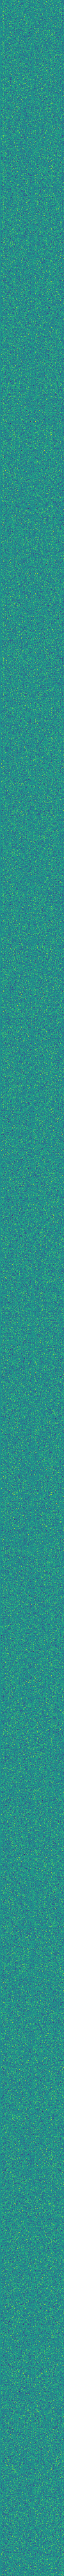
\includegraphics[interpolate=false,width=1.000000in,height=1.000000in]{antiderivative_ci_50-img0.png}}%
\end{pgfscope}%
\begin{pgfscope}%
\pgfsetbuttcap%
\pgfsetroundjoin%
\definecolor{currentfill}{rgb}{0.000000,0.000000,0.000000}%
\pgfsetfillcolor{currentfill}%
\pgfsetlinewidth{0.803000pt}%
\definecolor{currentstroke}{rgb}{0.000000,0.000000,0.000000}%
\pgfsetstrokecolor{currentstroke}%
\pgfsetdash{}{0pt}%
\pgfsys@defobject{currentmarker}{\pgfqpoint{0.000000in}{-0.048611in}}{\pgfqpoint{0.000000in}{0.000000in}}{%
\pgfpathmoveto{\pgfqpoint{0.000000in}{0.000000in}}%
\pgfpathlineto{\pgfqpoint{0.000000in}{-0.048611in}}%
\pgfusepath{stroke,fill}%
}%
\begin{pgfscope}%
\pgfsys@transformshift{0.800000in}{0.528000in}%
\pgfsys@useobject{currentmarker}{}%
\end{pgfscope}%
\end{pgfscope}%
\begin{pgfscope}%
\definecolor{textcolor}{rgb}{0.000000,0.000000,0.000000}%
\pgfsetstrokecolor{textcolor}%
\pgfsetfillcolor{textcolor}%
\pgftext[x=0.800000in,y=0.430778in,,top]{\color{textcolor}{\rmfamily\fontsize{12.000000}{14.400000}\selectfont\catcode`\^=\active\def^{\ifmmode\sp\else\^{}\fi}\catcode`\%=\active\def%{\%}0}}%
\end{pgfscope}%
\begin{pgfscope}%
\pgfsetbuttcap%
\pgfsetroundjoin%
\definecolor{currentfill}{rgb}{0.000000,0.000000,0.000000}%
\pgfsetfillcolor{currentfill}%
\pgfsetlinewidth{0.803000pt}%
\definecolor{currentstroke}{rgb}{0.000000,0.000000,0.000000}%
\pgfsetstrokecolor{currentstroke}%
\pgfsetdash{}{0pt}%
\pgfsys@defobject{currentmarker}{\pgfqpoint{0.000000in}{-0.048611in}}{\pgfqpoint{0.000000in}{0.000000in}}{%
\pgfpathmoveto{\pgfqpoint{0.000000in}{0.000000in}}%
\pgfpathlineto{\pgfqpoint{0.000000in}{-0.048611in}}%
\pgfusepath{stroke,fill}%
}%
\begin{pgfscope}%
\pgfsys@transformshift{1.593600in}{0.528000in}%
\pgfsys@useobject{currentmarker}{}%
\end{pgfscope}%
\end{pgfscope}%
\begin{pgfscope}%
\definecolor{textcolor}{rgb}{0.000000,0.000000,0.000000}%
\pgfsetstrokecolor{textcolor}%
\pgfsetfillcolor{textcolor}%
\pgftext[x=1.593600in,y=0.430778in,,top]{\color{textcolor}{\rmfamily\fontsize{12.000000}{14.400000}\selectfont\catcode`\^=\active\def^{\ifmmode\sp\else\^{}\fi}\catcode`\%=\active\def%{\%}10}}%
\end{pgfscope}%
\begin{pgfscope}%
\pgfsetbuttcap%
\pgfsetroundjoin%
\definecolor{currentfill}{rgb}{0.000000,0.000000,0.000000}%
\pgfsetfillcolor{currentfill}%
\pgfsetlinewidth{0.803000pt}%
\definecolor{currentstroke}{rgb}{0.000000,0.000000,0.000000}%
\pgfsetstrokecolor{currentstroke}%
\pgfsetdash{}{0pt}%
\pgfsys@defobject{currentmarker}{\pgfqpoint{0.000000in}{-0.048611in}}{\pgfqpoint{0.000000in}{0.000000in}}{%
\pgfpathmoveto{\pgfqpoint{0.000000in}{0.000000in}}%
\pgfpathlineto{\pgfqpoint{0.000000in}{-0.048611in}}%
\pgfusepath{stroke,fill}%
}%
\begin{pgfscope}%
\pgfsys@transformshift{2.387200in}{0.528000in}%
\pgfsys@useobject{currentmarker}{}%
\end{pgfscope}%
\end{pgfscope}%
\begin{pgfscope}%
\definecolor{textcolor}{rgb}{0.000000,0.000000,0.000000}%
\pgfsetstrokecolor{textcolor}%
\pgfsetfillcolor{textcolor}%
\pgftext[x=2.387200in,y=0.430778in,,top]{\color{textcolor}{\rmfamily\fontsize{12.000000}{14.400000}\selectfont\catcode`\^=\active\def^{\ifmmode\sp\else\^{}\fi}\catcode`\%=\active\def%{\%}20}}%
\end{pgfscope}%
\begin{pgfscope}%
\pgfsetbuttcap%
\pgfsetroundjoin%
\definecolor{currentfill}{rgb}{0.000000,0.000000,0.000000}%
\pgfsetfillcolor{currentfill}%
\pgfsetlinewidth{0.803000pt}%
\definecolor{currentstroke}{rgb}{0.000000,0.000000,0.000000}%
\pgfsetstrokecolor{currentstroke}%
\pgfsetdash{}{0pt}%
\pgfsys@defobject{currentmarker}{\pgfqpoint{0.000000in}{-0.048611in}}{\pgfqpoint{0.000000in}{0.000000in}}{%
\pgfpathmoveto{\pgfqpoint{0.000000in}{0.000000in}}%
\pgfpathlineto{\pgfqpoint{0.000000in}{-0.048611in}}%
\pgfusepath{stroke,fill}%
}%
\begin{pgfscope}%
\pgfsys@transformshift{3.180800in}{0.528000in}%
\pgfsys@useobject{currentmarker}{}%
\end{pgfscope}%
\end{pgfscope}%
\begin{pgfscope}%
\definecolor{textcolor}{rgb}{0.000000,0.000000,0.000000}%
\pgfsetstrokecolor{textcolor}%
\pgfsetfillcolor{textcolor}%
\pgftext[x=3.180800in,y=0.430778in,,top]{\color{textcolor}{\rmfamily\fontsize{12.000000}{14.400000}\selectfont\catcode`\^=\active\def^{\ifmmode\sp\else\^{}\fi}\catcode`\%=\active\def%{\%}30}}%
\end{pgfscope}%
\begin{pgfscope}%
\pgfsetbuttcap%
\pgfsetroundjoin%
\definecolor{currentfill}{rgb}{0.000000,0.000000,0.000000}%
\pgfsetfillcolor{currentfill}%
\pgfsetlinewidth{0.803000pt}%
\definecolor{currentstroke}{rgb}{0.000000,0.000000,0.000000}%
\pgfsetstrokecolor{currentstroke}%
\pgfsetdash{}{0pt}%
\pgfsys@defobject{currentmarker}{\pgfqpoint{0.000000in}{-0.048611in}}{\pgfqpoint{0.000000in}{0.000000in}}{%
\pgfpathmoveto{\pgfqpoint{0.000000in}{0.000000in}}%
\pgfpathlineto{\pgfqpoint{0.000000in}{-0.048611in}}%
\pgfusepath{stroke,fill}%
}%
\begin{pgfscope}%
\pgfsys@transformshift{3.974400in}{0.528000in}%
\pgfsys@useobject{currentmarker}{}%
\end{pgfscope}%
\end{pgfscope}%
\begin{pgfscope}%
\definecolor{textcolor}{rgb}{0.000000,0.000000,0.000000}%
\pgfsetstrokecolor{textcolor}%
\pgfsetfillcolor{textcolor}%
\pgftext[x=3.974400in,y=0.430778in,,top]{\color{textcolor}{\rmfamily\fontsize{12.000000}{14.400000}\selectfont\catcode`\^=\active\def^{\ifmmode\sp\else\^{}\fi}\catcode`\%=\active\def%{\%}40}}%
\end{pgfscope}%
\begin{pgfscope}%
\pgfsetbuttcap%
\pgfsetroundjoin%
\definecolor{currentfill}{rgb}{0.000000,0.000000,0.000000}%
\pgfsetfillcolor{currentfill}%
\pgfsetlinewidth{0.803000pt}%
\definecolor{currentstroke}{rgb}{0.000000,0.000000,0.000000}%
\pgfsetstrokecolor{currentstroke}%
\pgfsetdash{}{0pt}%
\pgfsys@defobject{currentmarker}{\pgfqpoint{0.000000in}{-0.048611in}}{\pgfqpoint{0.000000in}{0.000000in}}{%
\pgfpathmoveto{\pgfqpoint{0.000000in}{0.000000in}}%
\pgfpathlineto{\pgfqpoint{0.000000in}{-0.048611in}}%
\pgfusepath{stroke,fill}%
}%
\begin{pgfscope}%
\pgfsys@transformshift{4.768000in}{0.528000in}%
\pgfsys@useobject{currentmarker}{}%
\end{pgfscope}%
\end{pgfscope}%
\begin{pgfscope}%
\definecolor{textcolor}{rgb}{0.000000,0.000000,0.000000}%
\pgfsetstrokecolor{textcolor}%
\pgfsetfillcolor{textcolor}%
\pgftext[x=4.768000in,y=0.430778in,,top]{\color{textcolor}{\rmfamily\fontsize{12.000000}{14.400000}\selectfont\catcode`\^=\active\def^{\ifmmode\sp\else\^{}\fi}\catcode`\%=\active\def%{\%}50}}%
\end{pgfscope}%
\begin{pgfscope}%
\definecolor{textcolor}{rgb}{0.000000,0.000000,0.000000}%
\pgfsetstrokecolor{textcolor}%
\pgfsetfillcolor{textcolor}%
\pgftext[x=2.784000in,y=0.213927in,,top]{\color{textcolor}{\rmfamily\fontsize{12.000000}{14.400000}\selectfont\catcode`\^=\active\def^{\ifmmode\sp\else\^{}\fi}\catcode`\%=\active\def%{\%}input coefficients}}%
\end{pgfscope}%
\begin{pgfscope}%
\pgfsetbuttcap%
\pgfsetroundjoin%
\definecolor{currentfill}{rgb}{0.000000,0.000000,0.000000}%
\pgfsetfillcolor{currentfill}%
\pgfsetlinewidth{0.803000pt}%
\definecolor{currentstroke}{rgb}{0.000000,0.000000,0.000000}%
\pgfsetstrokecolor{currentstroke}%
\pgfsetdash{}{0pt}%
\pgfsys@defobject{currentmarker}{\pgfqpoint{-0.048611in}{0.000000in}}{\pgfqpoint{-0.000000in}{0.000000in}}{%
\pgfpathmoveto{\pgfqpoint{-0.000000in}{0.000000in}}%
\pgfpathlineto{\pgfqpoint{-0.048611in}{0.000000in}}%
\pgfusepath{stroke,fill}%
}%
\begin{pgfscope}%
\pgfsys@transformshift{0.800000in}{4.224000in}%
\pgfsys@useobject{currentmarker}{}%
\end{pgfscope}%
\end{pgfscope}%
\begin{pgfscope}%
\definecolor{textcolor}{rgb}{0.000000,0.000000,0.000000}%
\pgfsetstrokecolor{textcolor}%
\pgfsetfillcolor{textcolor}%
\pgftext[x=0.596739in, y=4.160686in, left, base]{\color{textcolor}{\rmfamily\fontsize{12.000000}{14.400000}\selectfont\catcode`\^=\active\def^{\ifmmode\sp\else\^{}\fi}\catcode`\%=\active\def%{\%}0}}%
\end{pgfscope}%
\begin{pgfscope}%
\pgfsetbuttcap%
\pgfsetroundjoin%
\definecolor{currentfill}{rgb}{0.000000,0.000000,0.000000}%
\pgfsetfillcolor{currentfill}%
\pgfsetlinewidth{0.803000pt}%
\definecolor{currentstroke}{rgb}{0.000000,0.000000,0.000000}%
\pgfsetstrokecolor{currentstroke}%
\pgfsetdash{}{0pt}%
\pgfsys@defobject{currentmarker}{\pgfqpoint{-0.048611in}{0.000000in}}{\pgfqpoint{-0.000000in}{0.000000in}}{%
\pgfpathmoveto{\pgfqpoint{-0.000000in}{0.000000in}}%
\pgfpathlineto{\pgfqpoint{-0.048611in}{0.000000in}}%
\pgfusepath{stroke,fill}%
}%
\begin{pgfscope}%
\pgfsys@transformshift{0.800000in}{3.762000in}%
\pgfsys@useobject{currentmarker}{}%
\end{pgfscope}%
\end{pgfscope}%
\begin{pgfscope}%
\definecolor{textcolor}{rgb}{0.000000,0.000000,0.000000}%
\pgfsetstrokecolor{textcolor}%
\pgfsetfillcolor{textcolor}%
\pgftext[x=0.384662in, y=3.698686in, left, base]{\color{textcolor}{\rmfamily\fontsize{12.000000}{14.400000}\selectfont\catcode`\^=\active\def^{\ifmmode\sp\else\^{}\fi}\catcode`\%=\active\def%{\%}500}}%
\end{pgfscope}%
\begin{pgfscope}%
\pgfsetbuttcap%
\pgfsetroundjoin%
\definecolor{currentfill}{rgb}{0.000000,0.000000,0.000000}%
\pgfsetfillcolor{currentfill}%
\pgfsetlinewidth{0.803000pt}%
\definecolor{currentstroke}{rgb}{0.000000,0.000000,0.000000}%
\pgfsetstrokecolor{currentstroke}%
\pgfsetdash{}{0pt}%
\pgfsys@defobject{currentmarker}{\pgfqpoint{-0.048611in}{0.000000in}}{\pgfqpoint{-0.000000in}{0.000000in}}{%
\pgfpathmoveto{\pgfqpoint{-0.000000in}{0.000000in}}%
\pgfpathlineto{\pgfqpoint{-0.048611in}{0.000000in}}%
\pgfusepath{stroke,fill}%
}%
\begin{pgfscope}%
\pgfsys@transformshift{0.800000in}{3.300000in}%
\pgfsys@useobject{currentmarker}{}%
\end{pgfscope}%
\end{pgfscope}%
\begin{pgfscope}%
\definecolor{textcolor}{rgb}{0.000000,0.000000,0.000000}%
\pgfsetstrokecolor{textcolor}%
\pgfsetfillcolor{textcolor}%
\pgftext[x=0.278624in, y=3.236686in, left, base]{\color{textcolor}{\rmfamily\fontsize{12.000000}{14.400000}\selectfont\catcode`\^=\active\def^{\ifmmode\sp\else\^{}\fi}\catcode`\%=\active\def%{\%}1000}}%
\end{pgfscope}%
\begin{pgfscope}%
\pgfsetbuttcap%
\pgfsetroundjoin%
\definecolor{currentfill}{rgb}{0.000000,0.000000,0.000000}%
\pgfsetfillcolor{currentfill}%
\pgfsetlinewidth{0.803000pt}%
\definecolor{currentstroke}{rgb}{0.000000,0.000000,0.000000}%
\pgfsetstrokecolor{currentstroke}%
\pgfsetdash{}{0pt}%
\pgfsys@defobject{currentmarker}{\pgfqpoint{-0.048611in}{0.000000in}}{\pgfqpoint{-0.000000in}{0.000000in}}{%
\pgfpathmoveto{\pgfqpoint{-0.000000in}{0.000000in}}%
\pgfpathlineto{\pgfqpoint{-0.048611in}{0.000000in}}%
\pgfusepath{stroke,fill}%
}%
\begin{pgfscope}%
\pgfsys@transformshift{0.800000in}{2.838000in}%
\pgfsys@useobject{currentmarker}{}%
\end{pgfscope}%
\end{pgfscope}%
\begin{pgfscope}%
\definecolor{textcolor}{rgb}{0.000000,0.000000,0.000000}%
\pgfsetstrokecolor{textcolor}%
\pgfsetfillcolor{textcolor}%
\pgftext[x=0.278624in, y=2.774686in, left, base]{\color{textcolor}{\rmfamily\fontsize{12.000000}{14.400000}\selectfont\catcode`\^=\active\def^{\ifmmode\sp\else\^{}\fi}\catcode`\%=\active\def%{\%}1500}}%
\end{pgfscope}%
\begin{pgfscope}%
\pgfsetbuttcap%
\pgfsetroundjoin%
\definecolor{currentfill}{rgb}{0.000000,0.000000,0.000000}%
\pgfsetfillcolor{currentfill}%
\pgfsetlinewidth{0.803000pt}%
\definecolor{currentstroke}{rgb}{0.000000,0.000000,0.000000}%
\pgfsetstrokecolor{currentstroke}%
\pgfsetdash{}{0pt}%
\pgfsys@defobject{currentmarker}{\pgfqpoint{-0.048611in}{0.000000in}}{\pgfqpoint{-0.000000in}{0.000000in}}{%
\pgfpathmoveto{\pgfqpoint{-0.000000in}{0.000000in}}%
\pgfpathlineto{\pgfqpoint{-0.048611in}{0.000000in}}%
\pgfusepath{stroke,fill}%
}%
\begin{pgfscope}%
\pgfsys@transformshift{0.800000in}{2.376000in}%
\pgfsys@useobject{currentmarker}{}%
\end{pgfscope}%
\end{pgfscope}%
\begin{pgfscope}%
\definecolor{textcolor}{rgb}{0.000000,0.000000,0.000000}%
\pgfsetstrokecolor{textcolor}%
\pgfsetfillcolor{textcolor}%
\pgftext[x=0.278624in, y=2.312686in, left, base]{\color{textcolor}{\rmfamily\fontsize{12.000000}{14.400000}\selectfont\catcode`\^=\active\def^{\ifmmode\sp\else\^{}\fi}\catcode`\%=\active\def%{\%}2000}}%
\end{pgfscope}%
\begin{pgfscope}%
\pgfsetbuttcap%
\pgfsetroundjoin%
\definecolor{currentfill}{rgb}{0.000000,0.000000,0.000000}%
\pgfsetfillcolor{currentfill}%
\pgfsetlinewidth{0.803000pt}%
\definecolor{currentstroke}{rgb}{0.000000,0.000000,0.000000}%
\pgfsetstrokecolor{currentstroke}%
\pgfsetdash{}{0pt}%
\pgfsys@defobject{currentmarker}{\pgfqpoint{-0.048611in}{0.000000in}}{\pgfqpoint{-0.000000in}{0.000000in}}{%
\pgfpathmoveto{\pgfqpoint{-0.000000in}{0.000000in}}%
\pgfpathlineto{\pgfqpoint{-0.048611in}{0.000000in}}%
\pgfusepath{stroke,fill}%
}%
\begin{pgfscope}%
\pgfsys@transformshift{0.800000in}{1.914000in}%
\pgfsys@useobject{currentmarker}{}%
\end{pgfscope}%
\end{pgfscope}%
\begin{pgfscope}%
\definecolor{textcolor}{rgb}{0.000000,0.000000,0.000000}%
\pgfsetstrokecolor{textcolor}%
\pgfsetfillcolor{textcolor}%
\pgftext[x=0.278624in, y=1.850686in, left, base]{\color{textcolor}{\rmfamily\fontsize{12.000000}{14.400000}\selectfont\catcode`\^=\active\def^{\ifmmode\sp\else\^{}\fi}\catcode`\%=\active\def%{\%}2500}}%
\end{pgfscope}%
\begin{pgfscope}%
\pgfsetbuttcap%
\pgfsetroundjoin%
\definecolor{currentfill}{rgb}{0.000000,0.000000,0.000000}%
\pgfsetfillcolor{currentfill}%
\pgfsetlinewidth{0.803000pt}%
\definecolor{currentstroke}{rgb}{0.000000,0.000000,0.000000}%
\pgfsetstrokecolor{currentstroke}%
\pgfsetdash{}{0pt}%
\pgfsys@defobject{currentmarker}{\pgfqpoint{-0.048611in}{0.000000in}}{\pgfqpoint{-0.000000in}{0.000000in}}{%
\pgfpathmoveto{\pgfqpoint{-0.000000in}{0.000000in}}%
\pgfpathlineto{\pgfqpoint{-0.048611in}{0.000000in}}%
\pgfusepath{stroke,fill}%
}%
\begin{pgfscope}%
\pgfsys@transformshift{0.800000in}{1.452000in}%
\pgfsys@useobject{currentmarker}{}%
\end{pgfscope}%
\end{pgfscope}%
\begin{pgfscope}%
\definecolor{textcolor}{rgb}{0.000000,0.000000,0.000000}%
\pgfsetstrokecolor{textcolor}%
\pgfsetfillcolor{textcolor}%
\pgftext[x=0.278624in, y=1.388686in, left, base]{\color{textcolor}{\rmfamily\fontsize{12.000000}{14.400000}\selectfont\catcode`\^=\active\def^{\ifmmode\sp\else\^{}\fi}\catcode`\%=\active\def%{\%}3000}}%
\end{pgfscope}%
\begin{pgfscope}%
\pgfsetbuttcap%
\pgfsetroundjoin%
\definecolor{currentfill}{rgb}{0.000000,0.000000,0.000000}%
\pgfsetfillcolor{currentfill}%
\pgfsetlinewidth{0.803000pt}%
\definecolor{currentstroke}{rgb}{0.000000,0.000000,0.000000}%
\pgfsetstrokecolor{currentstroke}%
\pgfsetdash{}{0pt}%
\pgfsys@defobject{currentmarker}{\pgfqpoint{-0.048611in}{0.000000in}}{\pgfqpoint{-0.000000in}{0.000000in}}{%
\pgfpathmoveto{\pgfqpoint{-0.000000in}{0.000000in}}%
\pgfpathlineto{\pgfqpoint{-0.048611in}{0.000000in}}%
\pgfusepath{stroke,fill}%
}%
\begin{pgfscope}%
\pgfsys@transformshift{0.800000in}{0.990000in}%
\pgfsys@useobject{currentmarker}{}%
\end{pgfscope}%
\end{pgfscope}%
\begin{pgfscope}%
\definecolor{textcolor}{rgb}{0.000000,0.000000,0.000000}%
\pgfsetstrokecolor{textcolor}%
\pgfsetfillcolor{textcolor}%
\pgftext[x=0.278624in, y=0.926686in, left, base]{\color{textcolor}{\rmfamily\fontsize{12.000000}{14.400000}\selectfont\catcode`\^=\active\def^{\ifmmode\sp\else\^{}\fi}\catcode`\%=\active\def%{\%}3500}}%
\end{pgfscope}%
\begin{pgfscope}%
\pgfsetbuttcap%
\pgfsetroundjoin%
\definecolor{currentfill}{rgb}{0.000000,0.000000,0.000000}%
\pgfsetfillcolor{currentfill}%
\pgfsetlinewidth{0.803000pt}%
\definecolor{currentstroke}{rgb}{0.000000,0.000000,0.000000}%
\pgfsetstrokecolor{currentstroke}%
\pgfsetdash{}{0pt}%
\pgfsys@defobject{currentmarker}{\pgfqpoint{-0.048611in}{0.000000in}}{\pgfqpoint{-0.000000in}{0.000000in}}{%
\pgfpathmoveto{\pgfqpoint{-0.000000in}{0.000000in}}%
\pgfpathlineto{\pgfqpoint{-0.048611in}{0.000000in}}%
\pgfusepath{stroke,fill}%
}%
\begin{pgfscope}%
\pgfsys@transformshift{0.800000in}{0.528000in}%
\pgfsys@useobject{currentmarker}{}%
\end{pgfscope}%
\end{pgfscope}%
\begin{pgfscope}%
\definecolor{textcolor}{rgb}{0.000000,0.000000,0.000000}%
\pgfsetstrokecolor{textcolor}%
\pgfsetfillcolor{textcolor}%
\pgftext[x=0.278624in, y=0.464686in, left, base]{\color{textcolor}{\rmfamily\fontsize{12.000000}{14.400000}\selectfont\catcode`\^=\active\def^{\ifmmode\sp\else\^{}\fi}\catcode`\%=\active\def%{\%}4000}}%
\end{pgfscope}%
\begin{pgfscope}%
\definecolor{textcolor}{rgb}{0.000000,0.000000,0.000000}%
\pgfsetstrokecolor{textcolor}%
\pgfsetfillcolor{textcolor}%
\pgftext[x=0.223069in,y=2.376000in,,bottom,rotate=90.000000]{\color{textcolor}{\rmfamily\fontsize{12.000000}{14.400000}\selectfont\catcode`\^=\active\def^{\ifmmode\sp\else\^{}\fi}\catcode`\%=\active\def%{\%}samples}}%
\end{pgfscope}%
\begin{pgfscope}%
\pgfsetrectcap%
\pgfsetmiterjoin%
\pgfsetlinewidth{0.803000pt}%
\definecolor{currentstroke}{rgb}{0.000000,0.000000,0.000000}%
\pgfsetstrokecolor{currentstroke}%
\pgfsetdash{}{0pt}%
\pgfpathmoveto{\pgfqpoint{0.800000in}{0.528000in}}%
\pgfpathlineto{\pgfqpoint{0.800000in}{4.224000in}}%
\pgfusepath{stroke}%
\end{pgfscope}%
\begin{pgfscope}%
\pgfsetrectcap%
\pgfsetmiterjoin%
\pgfsetlinewidth{0.803000pt}%
\definecolor{currentstroke}{rgb}{0.000000,0.000000,0.000000}%
\pgfsetstrokecolor{currentstroke}%
\pgfsetdash{}{0pt}%
\pgfpathmoveto{\pgfqpoint{4.768000in}{0.528000in}}%
\pgfpathlineto{\pgfqpoint{4.768000in}{4.224000in}}%
\pgfusepath{stroke}%
\end{pgfscope}%
\begin{pgfscope}%
\pgfsetrectcap%
\pgfsetmiterjoin%
\pgfsetlinewidth{0.803000pt}%
\definecolor{currentstroke}{rgb}{0.000000,0.000000,0.000000}%
\pgfsetstrokecolor{currentstroke}%
\pgfsetdash{}{0pt}%
\pgfpathmoveto{\pgfqpoint{0.800000in}{0.528000in}}%
\pgfpathlineto{\pgfqpoint{4.768000in}{0.528000in}}%
\pgfusepath{stroke}%
\end{pgfscope}%
\begin{pgfscope}%
\pgfsetrectcap%
\pgfsetmiterjoin%
\pgfsetlinewidth{0.803000pt}%
\definecolor{currentstroke}{rgb}{0.000000,0.000000,0.000000}%
\pgfsetstrokecolor{currentstroke}%
\pgfsetdash{}{0pt}%
\pgfpathmoveto{\pgfqpoint{0.800000in}{4.224000in}}%
\pgfpathlineto{\pgfqpoint{4.768000in}{4.224000in}}%
\pgfusepath{stroke}%
\end{pgfscope}%
\begin{pgfscope}%
\pgfsetbuttcap%
\pgfsetmiterjoin%
\pgfsetlinewidth{0.000000pt}%
\definecolor{currentstroke}{rgb}{0.000000,0.000000,0.000000}%
\pgfsetstrokecolor{currentstroke}%
\pgfsetstrokeopacity{0.000000}%
\pgfsetdash{}{0pt}%
\pgfpathmoveto{\pgfqpoint{5.016000in}{0.528000in}}%
\pgfpathlineto{\pgfqpoint{5.200800in}{0.528000in}}%
\pgfpathlineto{\pgfqpoint{5.200800in}{4.224000in}}%
\pgfpathlineto{\pgfqpoint{5.016000in}{4.224000in}}%
\pgfpathlineto{\pgfqpoint{5.016000in}{0.528000in}}%
\pgfpathclose%
\pgfusepath{}%
\end{pgfscope}%
\begin{pgfscope}%
\pgfsys@transformshift{5.020000in}{0.530000in}%
\pgftext[left,bottom]{
\includegraphics[interpolate=true,width=0.180000in,height=3.690000in]{antiderivative_ci_50-img1.png}}%
\end{pgfscope}%
\begin{pgfscope}%
\pgfsetbuttcap%
\pgfsetroundjoin%
\definecolor{currentfill}{rgb}{0.000000,0.000000,0.000000}%
\pgfsetfillcolor{currentfill}%
\pgfsetlinewidth{0.803000pt}%
\definecolor{currentstroke}{rgb}{0.000000,0.000000,0.000000}%
\pgfsetstrokecolor{currentstroke}%
\pgfsetdash{}{0pt}%
\pgfsys@defobject{currentmarker}{\pgfqpoint{0.000000in}{0.000000in}}{\pgfqpoint{0.048611in}{0.000000in}}{%
\pgfpathmoveto{\pgfqpoint{0.000000in}{0.000000in}}%
\pgfpathlineto{\pgfqpoint{0.048611in}{0.000000in}}%
\pgfusepath{stroke,fill}%
}%
\begin{pgfscope}%
\pgfsys@transformshift{5.200800in}{0.540424in}%
\pgfsys@useobject{currentmarker}{}%
\end{pgfscope}%
\end{pgfscope}%
\begin{pgfscope}%
\definecolor{textcolor}{rgb}{0.000000,0.000000,0.000000}%
\pgfsetstrokecolor{textcolor}%
\pgfsetfillcolor{textcolor}%
\pgftext[x=5.298022in, y=0.477110in, left, base]{\color{textcolor}{\rmfamily\fontsize{12.000000}{14.400000}\selectfont\catcode`\^=\active\def^{\ifmmode\sp\else\^{}\fi}\catcode`\%=\active\def%{\%}\ensuremath{-}100}}%
\end{pgfscope}%
\begin{pgfscope}%
\pgfsetbuttcap%
\pgfsetroundjoin%
\definecolor{currentfill}{rgb}{0.000000,0.000000,0.000000}%
\pgfsetfillcolor{currentfill}%
\pgfsetlinewidth{0.803000pt}%
\definecolor{currentstroke}{rgb}{0.000000,0.000000,0.000000}%
\pgfsetstrokecolor{currentstroke}%
\pgfsetdash{}{0pt}%
\pgfsys@defobject{currentmarker}{\pgfqpoint{0.000000in}{0.000000in}}{\pgfqpoint{0.048611in}{0.000000in}}{%
\pgfpathmoveto{\pgfqpoint{0.000000in}{0.000000in}}%
\pgfpathlineto{\pgfqpoint{0.048611in}{0.000000in}}%
\pgfusepath{stroke,fill}%
}%
\begin{pgfscope}%
\pgfsys@transformshift{5.200800in}{0.999318in}%
\pgfsys@useobject{currentmarker}{}%
\end{pgfscope}%
\end{pgfscope}%
\begin{pgfscope}%
\definecolor{textcolor}{rgb}{0.000000,0.000000,0.000000}%
\pgfsetstrokecolor{textcolor}%
\pgfsetfillcolor{textcolor}%
\pgftext[x=5.298022in, y=0.936004in, left, base]{\color{textcolor}{\rmfamily\fontsize{12.000000}{14.400000}\selectfont\catcode`\^=\active\def^{\ifmmode\sp\else\^{}\fi}\catcode`\%=\active\def%{\%}\ensuremath{-}75}}%
\end{pgfscope}%
\begin{pgfscope}%
\pgfsetbuttcap%
\pgfsetroundjoin%
\definecolor{currentfill}{rgb}{0.000000,0.000000,0.000000}%
\pgfsetfillcolor{currentfill}%
\pgfsetlinewidth{0.803000pt}%
\definecolor{currentstroke}{rgb}{0.000000,0.000000,0.000000}%
\pgfsetstrokecolor{currentstroke}%
\pgfsetdash{}{0pt}%
\pgfsys@defobject{currentmarker}{\pgfqpoint{0.000000in}{0.000000in}}{\pgfqpoint{0.048611in}{0.000000in}}{%
\pgfpathmoveto{\pgfqpoint{0.000000in}{0.000000in}}%
\pgfpathlineto{\pgfqpoint{0.048611in}{0.000000in}}%
\pgfusepath{stroke,fill}%
}%
\begin{pgfscope}%
\pgfsys@transformshift{5.200800in}{1.458212in}%
\pgfsys@useobject{currentmarker}{}%
\end{pgfscope}%
\end{pgfscope}%
\begin{pgfscope}%
\definecolor{textcolor}{rgb}{0.000000,0.000000,0.000000}%
\pgfsetstrokecolor{textcolor}%
\pgfsetfillcolor{textcolor}%
\pgftext[x=5.298022in, y=1.394898in, left, base]{\color{textcolor}{\rmfamily\fontsize{12.000000}{14.400000}\selectfont\catcode`\^=\active\def^{\ifmmode\sp\else\^{}\fi}\catcode`\%=\active\def%{\%}\ensuremath{-}50}}%
\end{pgfscope}%
\begin{pgfscope}%
\pgfsetbuttcap%
\pgfsetroundjoin%
\definecolor{currentfill}{rgb}{0.000000,0.000000,0.000000}%
\pgfsetfillcolor{currentfill}%
\pgfsetlinewidth{0.803000pt}%
\definecolor{currentstroke}{rgb}{0.000000,0.000000,0.000000}%
\pgfsetstrokecolor{currentstroke}%
\pgfsetdash{}{0pt}%
\pgfsys@defobject{currentmarker}{\pgfqpoint{0.000000in}{0.000000in}}{\pgfqpoint{0.048611in}{0.000000in}}{%
\pgfpathmoveto{\pgfqpoint{0.000000in}{0.000000in}}%
\pgfpathlineto{\pgfqpoint{0.048611in}{0.000000in}}%
\pgfusepath{stroke,fill}%
}%
\begin{pgfscope}%
\pgfsys@transformshift{5.200800in}{1.917106in}%
\pgfsys@useobject{currentmarker}{}%
\end{pgfscope}%
\end{pgfscope}%
\begin{pgfscope}%
\definecolor{textcolor}{rgb}{0.000000,0.000000,0.000000}%
\pgfsetstrokecolor{textcolor}%
\pgfsetfillcolor{textcolor}%
\pgftext[x=5.298022in, y=1.853792in, left, base]{\color{textcolor}{\rmfamily\fontsize{12.000000}{14.400000}\selectfont\catcode`\^=\active\def^{\ifmmode\sp\else\^{}\fi}\catcode`\%=\active\def%{\%}\ensuremath{-}25}}%
\end{pgfscope}%
\begin{pgfscope}%
\pgfsetbuttcap%
\pgfsetroundjoin%
\definecolor{currentfill}{rgb}{0.000000,0.000000,0.000000}%
\pgfsetfillcolor{currentfill}%
\pgfsetlinewidth{0.803000pt}%
\definecolor{currentstroke}{rgb}{0.000000,0.000000,0.000000}%
\pgfsetstrokecolor{currentstroke}%
\pgfsetdash{}{0pt}%
\pgfsys@defobject{currentmarker}{\pgfqpoint{0.000000in}{0.000000in}}{\pgfqpoint{0.048611in}{0.000000in}}{%
\pgfpathmoveto{\pgfqpoint{0.000000in}{0.000000in}}%
\pgfpathlineto{\pgfqpoint{0.048611in}{0.000000in}}%
\pgfusepath{stroke,fill}%
}%
\begin{pgfscope}%
\pgfsys@transformshift{5.200800in}{2.376000in}%
\pgfsys@useobject{currentmarker}{}%
\end{pgfscope}%
\end{pgfscope}%
\begin{pgfscope}%
\definecolor{textcolor}{rgb}{0.000000,0.000000,0.000000}%
\pgfsetstrokecolor{textcolor}%
\pgfsetfillcolor{textcolor}%
\pgftext[x=5.298022in, y=2.312686in, left, base]{\color{textcolor}{\rmfamily\fontsize{12.000000}{14.400000}\selectfont\catcode`\^=\active\def^{\ifmmode\sp\else\^{}\fi}\catcode`\%=\active\def%{\%}0}}%
\end{pgfscope}%
\begin{pgfscope}%
\pgfsetbuttcap%
\pgfsetroundjoin%
\definecolor{currentfill}{rgb}{0.000000,0.000000,0.000000}%
\pgfsetfillcolor{currentfill}%
\pgfsetlinewidth{0.803000pt}%
\definecolor{currentstroke}{rgb}{0.000000,0.000000,0.000000}%
\pgfsetstrokecolor{currentstroke}%
\pgfsetdash{}{0pt}%
\pgfsys@defobject{currentmarker}{\pgfqpoint{0.000000in}{0.000000in}}{\pgfqpoint{0.048611in}{0.000000in}}{%
\pgfpathmoveto{\pgfqpoint{0.000000in}{0.000000in}}%
\pgfpathlineto{\pgfqpoint{0.048611in}{0.000000in}}%
\pgfusepath{stroke,fill}%
}%
\begin{pgfscope}%
\pgfsys@transformshift{5.200800in}{2.834894in}%
\pgfsys@useobject{currentmarker}{}%
\end{pgfscope}%
\end{pgfscope}%
\begin{pgfscope}%
\definecolor{textcolor}{rgb}{0.000000,0.000000,0.000000}%
\pgfsetstrokecolor{textcolor}%
\pgfsetfillcolor{textcolor}%
\pgftext[x=5.298022in, y=2.771580in, left, base]{\color{textcolor}{\rmfamily\fontsize{12.000000}{14.400000}\selectfont\catcode`\^=\active\def^{\ifmmode\sp\else\^{}\fi}\catcode`\%=\active\def%{\%}25}}%
\end{pgfscope}%
\begin{pgfscope}%
\pgfsetbuttcap%
\pgfsetroundjoin%
\definecolor{currentfill}{rgb}{0.000000,0.000000,0.000000}%
\pgfsetfillcolor{currentfill}%
\pgfsetlinewidth{0.803000pt}%
\definecolor{currentstroke}{rgb}{0.000000,0.000000,0.000000}%
\pgfsetstrokecolor{currentstroke}%
\pgfsetdash{}{0pt}%
\pgfsys@defobject{currentmarker}{\pgfqpoint{0.000000in}{0.000000in}}{\pgfqpoint{0.048611in}{0.000000in}}{%
\pgfpathmoveto{\pgfqpoint{0.000000in}{0.000000in}}%
\pgfpathlineto{\pgfqpoint{0.048611in}{0.000000in}}%
\pgfusepath{stroke,fill}%
}%
\begin{pgfscope}%
\pgfsys@transformshift{5.200800in}{3.293788in}%
\pgfsys@useobject{currentmarker}{}%
\end{pgfscope}%
\end{pgfscope}%
\begin{pgfscope}%
\definecolor{textcolor}{rgb}{0.000000,0.000000,0.000000}%
\pgfsetstrokecolor{textcolor}%
\pgfsetfillcolor{textcolor}%
\pgftext[x=5.298022in, y=3.230474in, left, base]{\color{textcolor}{\rmfamily\fontsize{12.000000}{14.400000}\selectfont\catcode`\^=\active\def^{\ifmmode\sp\else\^{}\fi}\catcode`\%=\active\def%{\%}50}}%
\end{pgfscope}%
\begin{pgfscope}%
\pgfsetbuttcap%
\pgfsetroundjoin%
\definecolor{currentfill}{rgb}{0.000000,0.000000,0.000000}%
\pgfsetfillcolor{currentfill}%
\pgfsetlinewidth{0.803000pt}%
\definecolor{currentstroke}{rgb}{0.000000,0.000000,0.000000}%
\pgfsetstrokecolor{currentstroke}%
\pgfsetdash{}{0pt}%
\pgfsys@defobject{currentmarker}{\pgfqpoint{0.000000in}{0.000000in}}{\pgfqpoint{0.048611in}{0.000000in}}{%
\pgfpathmoveto{\pgfqpoint{0.000000in}{0.000000in}}%
\pgfpathlineto{\pgfqpoint{0.048611in}{0.000000in}}%
\pgfusepath{stroke,fill}%
}%
\begin{pgfscope}%
\pgfsys@transformshift{5.200800in}{3.752682in}%
\pgfsys@useobject{currentmarker}{}%
\end{pgfscope}%
\end{pgfscope}%
\begin{pgfscope}%
\definecolor{textcolor}{rgb}{0.000000,0.000000,0.000000}%
\pgfsetstrokecolor{textcolor}%
\pgfsetfillcolor{textcolor}%
\pgftext[x=5.298022in, y=3.689368in, left, base]{\color{textcolor}{\rmfamily\fontsize{12.000000}{14.400000}\selectfont\catcode`\^=\active\def^{\ifmmode\sp\else\^{}\fi}\catcode`\%=\active\def%{\%}75}}%
\end{pgfscope}%
\begin{pgfscope}%
\pgfsetbuttcap%
\pgfsetroundjoin%
\definecolor{currentfill}{rgb}{0.000000,0.000000,0.000000}%
\pgfsetfillcolor{currentfill}%
\pgfsetlinewidth{0.803000pt}%
\definecolor{currentstroke}{rgb}{0.000000,0.000000,0.000000}%
\pgfsetstrokecolor{currentstroke}%
\pgfsetdash{}{0pt}%
\pgfsys@defobject{currentmarker}{\pgfqpoint{0.000000in}{0.000000in}}{\pgfqpoint{0.048611in}{0.000000in}}{%
\pgfpathmoveto{\pgfqpoint{0.000000in}{0.000000in}}%
\pgfpathlineto{\pgfqpoint{0.048611in}{0.000000in}}%
\pgfusepath{stroke,fill}%
}%
\begin{pgfscope}%
\pgfsys@transformshift{5.200800in}{4.211576in}%
\pgfsys@useobject{currentmarker}{}%
\end{pgfscope}%
\end{pgfscope}%
\begin{pgfscope}%
\definecolor{textcolor}{rgb}{0.000000,0.000000,0.000000}%
\pgfsetstrokecolor{textcolor}%
\pgfsetfillcolor{textcolor}%
\pgftext[x=5.298022in, y=4.148262in, left, base]{\color{textcolor}{\rmfamily\fontsize{12.000000}{14.400000}\selectfont\catcode`\^=\active\def^{\ifmmode\sp\else\^{}\fi}\catcode`\%=\active\def%{\%}100}}%
\end{pgfscope}%
\begin{pgfscope}%
\pgfsetrectcap%
\pgfsetmiterjoin%
\pgfsetlinewidth{0.803000pt}%
\definecolor{currentstroke}{rgb}{0.000000,0.000000,0.000000}%
\pgfsetstrokecolor{currentstroke}%
\pgfsetdash{}{0pt}%
\pgfpathmoveto{\pgfqpoint{5.016000in}{0.528000in}}%
\pgfpathlineto{\pgfqpoint{5.108400in}{0.528000in}}%
\pgfpathlineto{\pgfqpoint{5.200800in}{0.528000in}}%
\pgfpathlineto{\pgfqpoint{5.200800in}{4.224000in}}%
\pgfpathlineto{\pgfqpoint{5.108400in}{4.224000in}}%
\pgfpathlineto{\pgfqpoint{5.016000in}{4.224000in}}%
\pgfpathlineto{\pgfqpoint{5.016000in}{0.528000in}}%
\pgfpathclose%
\pgfusepath{stroke}%
\end{pgfscope}%
\end{pgfpicture}%
\makeatother%
\endgroup%

      \end{adjustbox}
      \caption{Correlation image 50\% noise.}\label{fig:sc1_ci_50}
    \end{subfigure}
    \begin{subfigure}{0.49\linewidth}
      \begin{adjustbox}{width=\linewidth}
        \begingroup%
\makeatletter%
\begin{pgfpicture}%
\pgfpathrectangle{\pgfpointorigin}{\pgfqpoint{4.000000in}{3.000000in}}%
\pgfusepath{use as bounding box, clip}%
\begin{pgfscope}%
\pgfsetbuttcap%
\pgfsetmiterjoin%
\pgfsetlinewidth{0.000000pt}%
\definecolor{currentstroke}{rgb}{0.000000,0.000000,0.000000}%
\pgfsetstrokecolor{currentstroke}%
\pgfsetstrokeopacity{0.000000}%
\pgfsetdash{}{0pt}%
\pgfpathmoveto{\pgfqpoint{0.000000in}{0.000000in}}%
\pgfpathlineto{\pgfqpoint{4.000000in}{0.000000in}}%
\pgfpathlineto{\pgfqpoint{4.000000in}{3.000000in}}%
\pgfpathlineto{\pgfqpoint{0.000000in}{3.000000in}}%
\pgfpathlineto{\pgfqpoint{0.000000in}{0.000000in}}%
\pgfpathclose%
\pgfusepath{}%
\end{pgfscope}%
\begin{pgfscope}%
\pgfsetbuttcap%
\pgfsetmiterjoin%
\pgfsetlinewidth{0.000000pt}%
\definecolor{currentstroke}{rgb}{0.000000,0.000000,0.000000}%
\pgfsetstrokecolor{currentstroke}%
\pgfsetstrokeopacity{0.000000}%
\pgfsetdash{}{0pt}%
\pgfpathmoveto{\pgfqpoint{0.642156in}{0.517039in}}%
\pgfpathlineto{\pgfqpoint{3.032083in}{0.517039in}}%
\pgfpathlineto{\pgfqpoint{3.032083in}{2.906966in}}%
\pgfpathlineto{\pgfqpoint{0.642156in}{2.906966in}}%
\pgfpathlineto{\pgfqpoint{0.642156in}{0.517039in}}%
\pgfpathclose%
\pgfusepath{}%
\end{pgfscope}%
\begin{pgfscope}%
\pgfpathrectangle{\pgfqpoint{0.642156in}{0.517039in}}{\pgfqpoint{2.389927in}{2.389927in}}%
\pgfusepath{clip}%
\pgfsys@transformcm{2.389927}{0.000000}{0.000000}{-2.389927}{0.642156in}{2.906966in}%
\pgftext[left,bottom]{
\includegraphics[interpolate=false,width=1.000000in,height=1.000000in]{antiderivative_pm_50-img0.png}}%
\end{pgfscope}%
\begin{pgfscope}%
\pgfsetbuttcap%
\pgfsetroundjoin%
\definecolor{currentfill}{rgb}{0.000000,0.000000,0.000000}%
\pgfsetfillcolor{currentfill}%
\pgfsetlinewidth{0.803000pt}%
\definecolor{currentstroke}{rgb}{0.000000,0.000000,0.000000}%
\pgfsetstrokecolor{currentstroke}%
\pgfsetdash{}{0pt}%
\pgfsys@defobject{currentmarker}{\pgfqpoint{0.000000in}{-0.048611in}}{\pgfqpoint{0.000000in}{0.000000in}}{%
\pgfpathmoveto{\pgfqpoint{0.000000in}{0.000000in}}%
\pgfpathlineto{\pgfqpoint{0.000000in}{-0.048611in}}%
\pgfusepath{stroke,fill}%
}%
\begin{pgfscope}%
\pgfsys@transformshift{0.654106in}{0.517039in}%
\pgfsys@useobject{currentmarker}{}%
\end{pgfscope}%
\end{pgfscope}%
\begin{pgfscope}%
\definecolor{textcolor}{rgb}{0.000000,0.000000,0.000000}%
\pgfsetstrokecolor{textcolor}%
\pgfsetfillcolor{textcolor}%
\pgftext[x=0.654106in,y=0.419816in,,top]{\color{textcolor}{\rmfamily\fontsize{12.000000}{14.400000}\selectfont\catcode`\^=\active\def^{\ifmmode\sp\else\^{}\fi}\catcode`\%=\active\def%{\%}0}}%
\end{pgfscope}%
\begin{pgfscope}%
\pgfsetbuttcap%
\pgfsetroundjoin%
\definecolor{currentfill}{rgb}{0.000000,0.000000,0.000000}%
\pgfsetfillcolor{currentfill}%
\pgfsetlinewidth{0.803000pt}%
\definecolor{currentstroke}{rgb}{0.000000,0.000000,0.000000}%
\pgfsetstrokecolor{currentstroke}%
\pgfsetdash{}{0pt}%
\pgfsys@defobject{currentmarker}{\pgfqpoint{0.000000in}{-0.048611in}}{\pgfqpoint{0.000000in}{0.000000in}}{%
\pgfpathmoveto{\pgfqpoint{0.000000in}{0.000000in}}%
\pgfpathlineto{\pgfqpoint{0.000000in}{-0.048611in}}%
\pgfusepath{stroke,fill}%
}%
\begin{pgfscope}%
\pgfsys@transformshift{1.251588in}{0.517039in}%
\pgfsys@useobject{currentmarker}{}%
\end{pgfscope}%
\end{pgfscope}%
\begin{pgfscope}%
\definecolor{textcolor}{rgb}{0.000000,0.000000,0.000000}%
\pgfsetstrokecolor{textcolor}%
\pgfsetfillcolor{textcolor}%
\pgftext[x=1.251588in,y=0.419816in,,top]{\color{textcolor}{\rmfamily\fontsize{12.000000}{14.400000}\selectfont\catcode`\^=\active\def^{\ifmmode\sp\else\^{}\fi}\catcode`\%=\active\def%{\%}25}}%
\end{pgfscope}%
\begin{pgfscope}%
\pgfsetbuttcap%
\pgfsetroundjoin%
\definecolor{currentfill}{rgb}{0.000000,0.000000,0.000000}%
\pgfsetfillcolor{currentfill}%
\pgfsetlinewidth{0.803000pt}%
\definecolor{currentstroke}{rgb}{0.000000,0.000000,0.000000}%
\pgfsetstrokecolor{currentstroke}%
\pgfsetdash{}{0pt}%
\pgfsys@defobject{currentmarker}{\pgfqpoint{0.000000in}{-0.048611in}}{\pgfqpoint{0.000000in}{0.000000in}}{%
\pgfpathmoveto{\pgfqpoint{0.000000in}{0.000000in}}%
\pgfpathlineto{\pgfqpoint{0.000000in}{-0.048611in}}%
\pgfusepath{stroke,fill}%
}%
\begin{pgfscope}%
\pgfsys@transformshift{1.849069in}{0.517039in}%
\pgfsys@useobject{currentmarker}{}%
\end{pgfscope}%
\end{pgfscope}%
\begin{pgfscope}%
\definecolor{textcolor}{rgb}{0.000000,0.000000,0.000000}%
\pgfsetstrokecolor{textcolor}%
\pgfsetfillcolor{textcolor}%
\pgftext[x=1.849069in,y=0.419816in,,top]{\color{textcolor}{\rmfamily\fontsize{12.000000}{14.400000}\selectfont\catcode`\^=\active\def^{\ifmmode\sp\else\^{}\fi}\catcode`\%=\active\def%{\%}50}}%
\end{pgfscope}%
\begin{pgfscope}%
\pgfsetbuttcap%
\pgfsetroundjoin%
\definecolor{currentfill}{rgb}{0.000000,0.000000,0.000000}%
\pgfsetfillcolor{currentfill}%
\pgfsetlinewidth{0.803000pt}%
\definecolor{currentstroke}{rgb}{0.000000,0.000000,0.000000}%
\pgfsetstrokecolor{currentstroke}%
\pgfsetdash{}{0pt}%
\pgfsys@defobject{currentmarker}{\pgfqpoint{0.000000in}{-0.048611in}}{\pgfqpoint{0.000000in}{0.000000in}}{%
\pgfpathmoveto{\pgfqpoint{0.000000in}{0.000000in}}%
\pgfpathlineto{\pgfqpoint{0.000000in}{-0.048611in}}%
\pgfusepath{stroke,fill}%
}%
\begin{pgfscope}%
\pgfsys@transformshift{2.446551in}{0.517039in}%
\pgfsys@useobject{currentmarker}{}%
\end{pgfscope}%
\end{pgfscope}%
\begin{pgfscope}%
\definecolor{textcolor}{rgb}{0.000000,0.000000,0.000000}%
\pgfsetstrokecolor{textcolor}%
\pgfsetfillcolor{textcolor}%
\pgftext[x=2.446551in,y=0.419816in,,top]{\color{textcolor}{\rmfamily\fontsize{12.000000}{14.400000}\selectfont\catcode`\^=\active\def^{\ifmmode\sp\else\^{}\fi}\catcode`\%=\active\def%{\%}75}}%
\end{pgfscope}%
\begin{pgfscope}%
\definecolor{textcolor}{rgb}{0.000000,0.000000,0.000000}%
\pgfsetstrokecolor{textcolor}%
\pgfsetfillcolor{textcolor}%
\pgftext[x=1.837120in,y=0.202965in,,top]{\color{textcolor}{\rmfamily\fontsize{12.000000}{14.400000}\selectfont\catcode`\^=\active\def^{\ifmmode\sp\else\^{}\fi}\catcode`\%=\active\def%{\%}output coefficients}}%
\end{pgfscope}%
\begin{pgfscope}%
\pgfsetbuttcap%
\pgfsetroundjoin%
\definecolor{currentfill}{rgb}{0.000000,0.000000,0.000000}%
\pgfsetfillcolor{currentfill}%
\pgfsetlinewidth{0.803000pt}%
\definecolor{currentstroke}{rgb}{0.000000,0.000000,0.000000}%
\pgfsetstrokecolor{currentstroke}%
\pgfsetdash{}{0pt}%
\pgfsys@defobject{currentmarker}{\pgfqpoint{-0.048611in}{0.000000in}}{\pgfqpoint{-0.000000in}{0.000000in}}{%
\pgfpathmoveto{\pgfqpoint{-0.000000in}{0.000000in}}%
\pgfpathlineto{\pgfqpoint{-0.048611in}{0.000000in}}%
\pgfusepath{stroke,fill}%
}%
\begin{pgfscope}%
\pgfsys@transformshift{0.642156in}{2.895016in}%
\pgfsys@useobject{currentmarker}{}%
\end{pgfscope}%
\end{pgfscope}%
\begin{pgfscope}%
\definecolor{textcolor}{rgb}{0.000000,0.000000,0.000000}%
\pgfsetstrokecolor{textcolor}%
\pgfsetfillcolor{textcolor}%
\pgftext[x=0.438896in, y=2.831702in, left, base]{\color{textcolor}{\rmfamily\fontsize{12.000000}{14.400000}\selectfont\catcode`\^=\active\def^{\ifmmode\sp\else\^{}\fi}\catcode`\%=\active\def%{\%}0}}%
\end{pgfscope}%
\begin{pgfscope}%
\pgfsetbuttcap%
\pgfsetroundjoin%
\definecolor{currentfill}{rgb}{0.000000,0.000000,0.000000}%
\pgfsetfillcolor{currentfill}%
\pgfsetlinewidth{0.803000pt}%
\definecolor{currentstroke}{rgb}{0.000000,0.000000,0.000000}%
\pgfsetstrokecolor{currentstroke}%
\pgfsetdash{}{0pt}%
\pgfsys@defobject{currentmarker}{\pgfqpoint{-0.048611in}{0.000000in}}{\pgfqpoint{-0.000000in}{0.000000in}}{%
\pgfpathmoveto{\pgfqpoint{-0.000000in}{0.000000in}}%
\pgfpathlineto{\pgfqpoint{-0.048611in}{0.000000in}}%
\pgfusepath{stroke,fill}%
}%
\begin{pgfscope}%
\pgfsys@transformshift{0.642156in}{2.417031in}%
\pgfsys@useobject{currentmarker}{}%
\end{pgfscope}%
\end{pgfscope}%
\begin{pgfscope}%
\definecolor{textcolor}{rgb}{0.000000,0.000000,0.000000}%
\pgfsetstrokecolor{textcolor}%
\pgfsetfillcolor{textcolor}%
\pgftext[x=0.332857in, y=2.353717in, left, base]{\color{textcolor}{\rmfamily\fontsize{12.000000}{14.400000}\selectfont\catcode`\^=\active\def^{\ifmmode\sp\else\^{}\fi}\catcode`\%=\active\def%{\%}20}}%
\end{pgfscope}%
\begin{pgfscope}%
\pgfsetbuttcap%
\pgfsetroundjoin%
\definecolor{currentfill}{rgb}{0.000000,0.000000,0.000000}%
\pgfsetfillcolor{currentfill}%
\pgfsetlinewidth{0.803000pt}%
\definecolor{currentstroke}{rgb}{0.000000,0.000000,0.000000}%
\pgfsetstrokecolor{currentstroke}%
\pgfsetdash{}{0pt}%
\pgfsys@defobject{currentmarker}{\pgfqpoint{-0.048611in}{0.000000in}}{\pgfqpoint{-0.000000in}{0.000000in}}{%
\pgfpathmoveto{\pgfqpoint{-0.000000in}{0.000000in}}%
\pgfpathlineto{\pgfqpoint{-0.048611in}{0.000000in}}%
\pgfusepath{stroke,fill}%
}%
\begin{pgfscope}%
\pgfsys@transformshift{0.642156in}{1.939045in}%
\pgfsys@useobject{currentmarker}{}%
\end{pgfscope}%
\end{pgfscope}%
\begin{pgfscope}%
\definecolor{textcolor}{rgb}{0.000000,0.000000,0.000000}%
\pgfsetstrokecolor{textcolor}%
\pgfsetfillcolor{textcolor}%
\pgftext[x=0.332857in, y=1.875731in, left, base]{\color{textcolor}{\rmfamily\fontsize{12.000000}{14.400000}\selectfont\catcode`\^=\active\def^{\ifmmode\sp\else\^{}\fi}\catcode`\%=\active\def%{\%}40}}%
\end{pgfscope}%
\begin{pgfscope}%
\pgfsetbuttcap%
\pgfsetroundjoin%
\definecolor{currentfill}{rgb}{0.000000,0.000000,0.000000}%
\pgfsetfillcolor{currentfill}%
\pgfsetlinewidth{0.803000pt}%
\definecolor{currentstroke}{rgb}{0.000000,0.000000,0.000000}%
\pgfsetstrokecolor{currentstroke}%
\pgfsetdash{}{0pt}%
\pgfsys@defobject{currentmarker}{\pgfqpoint{-0.048611in}{0.000000in}}{\pgfqpoint{-0.000000in}{0.000000in}}{%
\pgfpathmoveto{\pgfqpoint{-0.000000in}{0.000000in}}%
\pgfpathlineto{\pgfqpoint{-0.048611in}{0.000000in}}%
\pgfusepath{stroke,fill}%
}%
\begin{pgfscope}%
\pgfsys@transformshift{0.642156in}{1.461060in}%
\pgfsys@useobject{currentmarker}{}%
\end{pgfscope}%
\end{pgfscope}%
\begin{pgfscope}%
\definecolor{textcolor}{rgb}{0.000000,0.000000,0.000000}%
\pgfsetstrokecolor{textcolor}%
\pgfsetfillcolor{textcolor}%
\pgftext[x=0.332857in, y=1.397746in, left, base]{\color{textcolor}{\rmfamily\fontsize{12.000000}{14.400000}\selectfont\catcode`\^=\active\def^{\ifmmode\sp\else\^{}\fi}\catcode`\%=\active\def%{\%}60}}%
\end{pgfscope}%
\begin{pgfscope}%
\pgfsetbuttcap%
\pgfsetroundjoin%
\definecolor{currentfill}{rgb}{0.000000,0.000000,0.000000}%
\pgfsetfillcolor{currentfill}%
\pgfsetlinewidth{0.803000pt}%
\definecolor{currentstroke}{rgb}{0.000000,0.000000,0.000000}%
\pgfsetstrokecolor{currentstroke}%
\pgfsetdash{}{0pt}%
\pgfsys@defobject{currentmarker}{\pgfqpoint{-0.048611in}{0.000000in}}{\pgfqpoint{-0.000000in}{0.000000in}}{%
\pgfpathmoveto{\pgfqpoint{-0.000000in}{0.000000in}}%
\pgfpathlineto{\pgfqpoint{-0.048611in}{0.000000in}}%
\pgfusepath{stroke,fill}%
}%
\begin{pgfscope}%
\pgfsys@transformshift{0.642156in}{0.983074in}%
\pgfsys@useobject{currentmarker}{}%
\end{pgfscope}%
\end{pgfscope}%
\begin{pgfscope}%
\definecolor{textcolor}{rgb}{0.000000,0.000000,0.000000}%
\pgfsetstrokecolor{textcolor}%
\pgfsetfillcolor{textcolor}%
\pgftext[x=0.332857in, y=0.919761in, left, base]{\color{textcolor}{\rmfamily\fontsize{12.000000}{14.400000}\selectfont\catcode`\^=\active\def^{\ifmmode\sp\else\^{}\fi}\catcode`\%=\active\def%{\%}80}}%
\end{pgfscope}%
\begin{pgfscope}%
\definecolor{textcolor}{rgb}{0.000000,0.000000,0.000000}%
\pgfsetstrokecolor{textcolor}%
\pgfsetfillcolor{textcolor}%
\pgftext[x=0.277302in,y=1.712002in,,bottom,rotate=90.000000]{\color{textcolor}{\rmfamily\fontsize{12.000000}{14.400000}\selectfont\catcode`\^=\active\def^{\ifmmode\sp\else\^{}\fi}\catcode`\%=\active\def%{\%}input coefficients}}%
\end{pgfscope}%
\begin{pgfscope}%
\pgfsetrectcap%
\pgfsetmiterjoin%
\pgfsetlinewidth{0.803000pt}%
\definecolor{currentstroke}{rgb}{0.000000,0.000000,0.000000}%
\pgfsetstrokecolor{currentstroke}%
\pgfsetdash{}{0pt}%
\pgfpathmoveto{\pgfqpoint{0.642156in}{0.517039in}}%
\pgfpathlineto{\pgfqpoint{0.642156in}{2.906966in}}%
\pgfusepath{stroke}%
\end{pgfscope}%
\begin{pgfscope}%
\pgfsetrectcap%
\pgfsetmiterjoin%
\pgfsetlinewidth{0.803000pt}%
\definecolor{currentstroke}{rgb}{0.000000,0.000000,0.000000}%
\pgfsetstrokecolor{currentstroke}%
\pgfsetdash{}{0pt}%
\pgfpathmoveto{\pgfqpoint{3.032083in}{0.517039in}}%
\pgfpathlineto{\pgfqpoint{3.032083in}{2.906966in}}%
\pgfusepath{stroke}%
\end{pgfscope}%
\begin{pgfscope}%
\pgfsetrectcap%
\pgfsetmiterjoin%
\pgfsetlinewidth{0.803000pt}%
\definecolor{currentstroke}{rgb}{0.000000,0.000000,0.000000}%
\pgfsetstrokecolor{currentstroke}%
\pgfsetdash{}{0pt}%
\pgfpathmoveto{\pgfqpoint{0.642156in}{0.517039in}}%
\pgfpathlineto{\pgfqpoint{3.032083in}{0.517039in}}%
\pgfusepath{stroke}%
\end{pgfscope}%
\begin{pgfscope}%
\pgfsetrectcap%
\pgfsetmiterjoin%
\pgfsetlinewidth{0.803000pt}%
\definecolor{currentstroke}{rgb}{0.000000,0.000000,0.000000}%
\pgfsetstrokecolor{currentstroke}%
\pgfsetdash{}{0pt}%
\pgfpathmoveto{\pgfqpoint{0.642156in}{2.906966in}}%
\pgfpathlineto{\pgfqpoint{3.032083in}{2.906966in}}%
\pgfusepath{stroke}%
\end{pgfscope}%
\begin{pgfscope}%
\pgfsetbuttcap%
\pgfsetmiterjoin%
\pgfsetlinewidth{0.000000pt}%
\definecolor{currentstroke}{rgb}{0.000000,0.000000,0.000000}%
\pgfsetstrokecolor{currentstroke}%
\pgfsetstrokeopacity{0.000000}%
\pgfsetdash{}{0pt}%
\pgfpathmoveto{\pgfqpoint{3.181604in}{0.517039in}}%
\pgfpathlineto{\pgfqpoint{3.301100in}{0.517039in}}%
\pgfpathlineto{\pgfqpoint{3.301100in}{2.906966in}}%
\pgfpathlineto{\pgfqpoint{3.181604in}{2.906966in}}%
\pgfpathlineto{\pgfqpoint{3.181604in}{0.517039in}}%
\pgfpathclose%
\pgfusepath{}%
\end{pgfscope}%
\begin{pgfscope}%
\pgfsys@transformshift{3.180000in}{0.520000in}%
\pgftext[left,bottom]{
\includegraphics[interpolate=true,width=0.120000in,height=2.390000in]{antiderivative_pm_50-img1.png}}%
\end{pgfscope}%
\begin{pgfscope}%
\pgfsetbuttcap%
\pgfsetroundjoin%
\definecolor{currentfill}{rgb}{0.000000,0.000000,0.000000}%
\pgfsetfillcolor{currentfill}%
\pgfsetlinewidth{0.803000pt}%
\definecolor{currentstroke}{rgb}{0.000000,0.000000,0.000000}%
\pgfsetstrokecolor{currentstroke}%
\pgfsetdash{}{0pt}%
\pgfsys@defobject{currentmarker}{\pgfqpoint{0.000000in}{0.000000in}}{\pgfqpoint{0.048611in}{0.000000in}}{%
\pgfpathmoveto{\pgfqpoint{0.000000in}{0.000000in}}%
\pgfpathlineto{\pgfqpoint{0.048611in}{0.000000in}}%
\pgfusepath{stroke,fill}%
}%
\begin{pgfscope}%
\pgfsys@transformshift{3.301100in}{0.707209in}%
\pgfsys@useobject{currentmarker}{}%
\end{pgfscope}%
\end{pgfscope}%
\begin{pgfscope}%
\definecolor{textcolor}{rgb}{0.000000,0.000000,0.000000}%
\pgfsetstrokecolor{textcolor}%
\pgfsetfillcolor{textcolor}%
\pgftext[x=3.398323in, y=0.643895in, left, base]{\color{textcolor}{\rmfamily\fontsize{12.000000}{14.400000}\selectfont\catcode`\^=\active\def^{\ifmmode\sp\else\^{}\fi}\catcode`\%=\active\def%{\%}\ensuremath{-}2000}}%
\end{pgfscope}%
\begin{pgfscope}%
\pgfsetbuttcap%
\pgfsetroundjoin%
\definecolor{currentfill}{rgb}{0.000000,0.000000,0.000000}%
\pgfsetfillcolor{currentfill}%
\pgfsetlinewidth{0.803000pt}%
\definecolor{currentstroke}{rgb}{0.000000,0.000000,0.000000}%
\pgfsetstrokecolor{currentstroke}%
\pgfsetdash{}{0pt}%
\pgfsys@defobject{currentmarker}{\pgfqpoint{0.000000in}{0.000000in}}{\pgfqpoint{0.048611in}{0.000000in}}{%
\pgfpathmoveto{\pgfqpoint{0.000000in}{0.000000in}}%
\pgfpathlineto{\pgfqpoint{0.048611in}{0.000000in}}%
\pgfusepath{stroke,fill}%
}%
\begin{pgfscope}%
\pgfsys@transformshift{3.301100in}{1.096875in}%
\pgfsys@useobject{currentmarker}{}%
\end{pgfscope}%
\end{pgfscope}%
\begin{pgfscope}%
\definecolor{textcolor}{rgb}{0.000000,0.000000,0.000000}%
\pgfsetstrokecolor{textcolor}%
\pgfsetfillcolor{textcolor}%
\pgftext[x=3.398323in, y=1.033561in, left, base]{\color{textcolor}{\rmfamily\fontsize{12.000000}{14.400000}\selectfont\catcode`\^=\active\def^{\ifmmode\sp\else\^{}\fi}\catcode`\%=\active\def%{\%}\ensuremath{-}1500}}%
\end{pgfscope}%
\begin{pgfscope}%
\pgfsetbuttcap%
\pgfsetroundjoin%
\definecolor{currentfill}{rgb}{0.000000,0.000000,0.000000}%
\pgfsetfillcolor{currentfill}%
\pgfsetlinewidth{0.803000pt}%
\definecolor{currentstroke}{rgb}{0.000000,0.000000,0.000000}%
\pgfsetstrokecolor{currentstroke}%
\pgfsetdash{}{0pt}%
\pgfsys@defobject{currentmarker}{\pgfqpoint{0.000000in}{0.000000in}}{\pgfqpoint{0.048611in}{0.000000in}}{%
\pgfpathmoveto{\pgfqpoint{0.000000in}{0.000000in}}%
\pgfpathlineto{\pgfqpoint{0.048611in}{0.000000in}}%
\pgfusepath{stroke,fill}%
}%
\begin{pgfscope}%
\pgfsys@transformshift{3.301100in}{1.486541in}%
\pgfsys@useobject{currentmarker}{}%
\end{pgfscope}%
\end{pgfscope}%
\begin{pgfscope}%
\definecolor{textcolor}{rgb}{0.000000,0.000000,0.000000}%
\pgfsetstrokecolor{textcolor}%
\pgfsetfillcolor{textcolor}%
\pgftext[x=3.398323in, y=1.423227in, left, base]{\color{textcolor}{\rmfamily\fontsize{12.000000}{14.400000}\selectfont\catcode`\^=\active\def^{\ifmmode\sp\else\^{}\fi}\catcode`\%=\active\def%{\%}\ensuremath{-}1000}}%
\end{pgfscope}%
\begin{pgfscope}%
\pgfsetbuttcap%
\pgfsetroundjoin%
\definecolor{currentfill}{rgb}{0.000000,0.000000,0.000000}%
\pgfsetfillcolor{currentfill}%
\pgfsetlinewidth{0.803000pt}%
\definecolor{currentstroke}{rgb}{0.000000,0.000000,0.000000}%
\pgfsetstrokecolor{currentstroke}%
\pgfsetdash{}{0pt}%
\pgfsys@defobject{currentmarker}{\pgfqpoint{0.000000in}{0.000000in}}{\pgfqpoint{0.048611in}{0.000000in}}{%
\pgfpathmoveto{\pgfqpoint{0.000000in}{0.000000in}}%
\pgfpathlineto{\pgfqpoint{0.048611in}{0.000000in}}%
\pgfusepath{stroke,fill}%
}%
\begin{pgfscope}%
\pgfsys@transformshift{3.301100in}{1.876208in}%
\pgfsys@useobject{currentmarker}{}%
\end{pgfscope}%
\end{pgfscope}%
\begin{pgfscope}%
\definecolor{textcolor}{rgb}{0.000000,0.000000,0.000000}%
\pgfsetstrokecolor{textcolor}%
\pgfsetfillcolor{textcolor}%
\pgftext[x=3.398323in, y=1.812894in, left, base]{\color{textcolor}{\rmfamily\fontsize{12.000000}{14.400000}\selectfont\catcode`\^=\active\def^{\ifmmode\sp\else\^{}\fi}\catcode`\%=\active\def%{\%}\ensuremath{-}500}}%
\end{pgfscope}%
\begin{pgfscope}%
\pgfsetbuttcap%
\pgfsetroundjoin%
\definecolor{currentfill}{rgb}{0.000000,0.000000,0.000000}%
\pgfsetfillcolor{currentfill}%
\pgfsetlinewidth{0.803000pt}%
\definecolor{currentstroke}{rgb}{0.000000,0.000000,0.000000}%
\pgfsetstrokecolor{currentstroke}%
\pgfsetdash{}{0pt}%
\pgfsys@defobject{currentmarker}{\pgfqpoint{0.000000in}{0.000000in}}{\pgfqpoint{0.048611in}{0.000000in}}{%
\pgfpathmoveto{\pgfqpoint{0.000000in}{0.000000in}}%
\pgfpathlineto{\pgfqpoint{0.048611in}{0.000000in}}%
\pgfusepath{stroke,fill}%
}%
\begin{pgfscope}%
\pgfsys@transformshift{3.301100in}{2.265874in}%
\pgfsys@useobject{currentmarker}{}%
\end{pgfscope}%
\end{pgfscope}%
\begin{pgfscope}%
\definecolor{textcolor}{rgb}{0.000000,0.000000,0.000000}%
\pgfsetstrokecolor{textcolor}%
\pgfsetfillcolor{textcolor}%
\pgftext[x=3.398323in, y=2.202560in, left, base]{\color{textcolor}{\rmfamily\fontsize{12.000000}{14.400000}\selectfont\catcode`\^=\active\def^{\ifmmode\sp\else\^{}\fi}\catcode`\%=\active\def%{\%}0}}%
\end{pgfscope}%
\begin{pgfscope}%
\pgfsetbuttcap%
\pgfsetroundjoin%
\definecolor{currentfill}{rgb}{0.000000,0.000000,0.000000}%
\pgfsetfillcolor{currentfill}%
\pgfsetlinewidth{0.803000pt}%
\definecolor{currentstroke}{rgb}{0.000000,0.000000,0.000000}%
\pgfsetstrokecolor{currentstroke}%
\pgfsetdash{}{0pt}%
\pgfsys@defobject{currentmarker}{\pgfqpoint{0.000000in}{0.000000in}}{\pgfqpoint{0.048611in}{0.000000in}}{%
\pgfpathmoveto{\pgfqpoint{0.000000in}{0.000000in}}%
\pgfpathlineto{\pgfqpoint{0.048611in}{0.000000in}}%
\pgfusepath{stroke,fill}%
}%
\begin{pgfscope}%
\pgfsys@transformshift{3.301100in}{2.655540in}%
\pgfsys@useobject{currentmarker}{}%
\end{pgfscope}%
\end{pgfscope}%
\begin{pgfscope}%
\definecolor{textcolor}{rgb}{0.000000,0.000000,0.000000}%
\pgfsetstrokecolor{textcolor}%
\pgfsetfillcolor{textcolor}%
\pgftext[x=3.398323in, y=2.592226in, left, base]{\color{textcolor}{\rmfamily\fontsize{12.000000}{14.400000}\selectfont\catcode`\^=\active\def^{\ifmmode\sp\else\^{}\fi}\catcode`\%=\active\def%{\%}500}}%
\end{pgfscope}%
\begin{pgfscope}%
\pgfsetrectcap%
\pgfsetmiterjoin%
\pgfsetlinewidth{0.803000pt}%
\definecolor{currentstroke}{rgb}{0.000000,0.000000,0.000000}%
\pgfsetstrokecolor{currentstroke}%
\pgfsetdash{}{0pt}%
\pgfpathmoveto{\pgfqpoint{3.181604in}{0.517039in}}%
\pgfpathlineto{\pgfqpoint{3.241352in}{0.517039in}}%
\pgfpathlineto{\pgfqpoint{3.301100in}{0.517039in}}%
\pgfpathlineto{\pgfqpoint{3.301100in}{2.906966in}}%
\pgfpathlineto{\pgfqpoint{3.241352in}{2.906966in}}%
\pgfpathlineto{\pgfqpoint{3.181604in}{2.906966in}}%
\pgfpathlineto{\pgfqpoint{3.181604in}{0.517039in}}%
\pgfpathclose%
\pgfusepath{stroke}%
\end{pgfscope}%
\end{pgfpicture}%
\makeatother%
\endgroup%

      \end{adjustbox}
      \caption{The p-matrix for 50\% noise.}\label{fig:sc1_pm_50}
    \end{subfigure}
  \end{adjustwidth}
  \caption{Correlation image (left column) and p-matrix (right column) for each model trained on a different noise level (row). The correlation image was sorted same order the values of the real component of wave number \(k=2\) were sorted in descending order.}\label{fig:scenario_1_interpretation}
\end{figure}

The final observation we make is how for all the p-matrices the pronounced contribution of the input wave number to their corresponding output wave number. This means that the majority of contributions to each output coefficients come from the corresponding input coefficients of the same wave number. Our knowledge on how the simple derivative equation for Fourier series relate the coefficients of the derivative function and the antiderivative function is shown in \lccref{eq:derivative_coeff}. This aligns with the contributions shown by the p-matrices. This confirms that the model is indeed learning the relations that is defined by the derivative equation.

In summary, the model is able to learn the linear relationship defined by the derivative equation. This is true even for high noise levels. The model also learns the actual relationship between each wave number which is shown in the p-matrix. Inverse prediction of the input function is also successfully done for lower noise levels. At high noise levels, the noise overwhelms the model.

\subsection{Scenario 2}
\noindent The second scenario results are presented in two parts which are the coefficient predictions and function value predictions. The functions are first preprocessed in order to format them into current and next values in time as discussed in \lccref{sec:data_transformation}. The sample pairs are first divided into two for the training and testing sets. Each function is then discretized into 200 time steps. Then, the features are put together as the coefficients of the solution and forcing term at the current time step. The labels are the solution at the next time step. Since there is too much data to fit into memory all at once at the end of this process, we randomly sample the feature and label pairs. This result in a maximum of 8000 samples for the training set and 2000 samples for the testing set. As mentioned in \lccref{sec:data_transformation}, the training features are used to fit a scaling function. And then, all features are scaled using the fitted scaling function.

The coefficient value predictions are shown in \lccref{table:scenario_2_spectral_metrics}. The RBF kernel parameter computed from the data is once again the same for all versions of the dataset with a value of 5.66. The testing metrics show that the performance of the model vary with the viscosity value \(\nu \). Starting with the inviscid Burgers' equation, with \(\nu=0\), the model performs the best with a close second from the model for the \(\nu = 0.01 \) dataset version. The function value evaluated from the predictions is shown in \lccref{table:scenario_2_function_metrics}. The metrics across the board shows that the function value relative metrics are slightly better compared to the coefficients. Comparing the absolute metrics for the same table, we see the same general trend that the higher viscosity show the model performing worse.

\begin{table}[H]
  \caption{Performance metrics of coefficient prediction of next time step in scenario 2 by viscosity.}\label{table:scenario_2_spectral_metrics}
  \centering
  \begin{tabular}{lrrrrr}
    \toprule
    \(\nu \) & MSE      & RMSE     & MAE      & R2   & sMAPE \\
    \midrule
    0.0      & 3.46e-04 & 1.86e-02 & 1.24e-02 & 0.79 & 0.65  \\
    0.01     & 3.56e-04 & 1.89e-02 & 1.27e-02 & 0.78 & 0.67  \\
    0.1      & 9.17e-04 & 3.03e-02 & 2.32e-02 & 0.46 & 1.08  \\
    \bottomrule
  \end{tabular}
\end{table}

\begin{table}[H]
  \caption{Performance metrics of function values evaluated from coefficient prediction of next time step in scenario 2 by viscosity.}\label{table:scenario_2_function_metrics}
  \centering
  \begin{tabular}{lrrrrr}
    \toprule
    \(\nu \) & MSE      & RMSE     & MAE      & R2   & sMAPE \\
    \midrule
    0.0      & 5.58e-05 & 7.47e-03 & 5.89e-03 & 0.82 & 0.70  \\
    0.01     & 5.74e-05 & 7.58e-03 & 6.01e-03 & 0.81 & 0.71  \\
    0.1      & 1.58e-04 & 1.26e-02 & 9.98e-03 & 0.51 & 1.04  \\
    \bottomrule
  \end{tabular}
\end{table}

The testing results are complimented with a rollout experiment. The results from the rollout are shown in \lccref{fig:scenario_2_rollout}. The rollout starts from time \(t=0\). In all the plots, this is at the bottom. We have included this initial condition in the plots. From this initial condition in combination with the forcing term at the initial time step, the model predicts the first time step solution. The model then uses the predicted solution combined with the corresponding forcing term to predict the second time step. To see how well the model is performing relative to the actual target values, we compute the difference between the two as shown in \lccrefs{fig:sc2_rollout_diff_0.0,fig:sc2_rollout_diff_0.01,fig:sc2_rollout_diff_0.1}. Observe that errors are introduced relatively early around time \(t=1\). However, the model rollout stays stable until the end despite this error. This results in the model being able to finish the rollout for this sample.
\begin{figure}[H]
  \centering
  \begin{adjustwidth}{-0.1\linewidth}{-0.1\linewidth}
    \begin{subfigure}{0.33\linewidth}
      \begin{adjustbox}{width=\linewidth}
        \begingroup%
\makeatletter%
\begin{pgfpicture}%
\pgfpathrectangle{\pgfpointorigin}{\pgfqpoint{3.000000in}{2.000000in}}%
\pgfusepath{use as bounding box, clip}%
\begin{pgfscope}%
\pgfsetbuttcap%
\pgfsetmiterjoin%
\pgfsetlinewidth{0.000000pt}%
\definecolor{currentstroke}{rgb}{0.000000,0.000000,0.000000}%
\pgfsetstrokecolor{currentstroke}%
\pgfsetstrokeopacity{0.000000}%
\pgfsetdash{}{0pt}%
\pgfpathmoveto{\pgfqpoint{0.000000in}{0.000000in}}%
\pgfpathlineto{\pgfqpoint{3.000000in}{0.000000in}}%
\pgfpathlineto{\pgfqpoint{3.000000in}{2.000000in}}%
\pgfpathlineto{\pgfqpoint{0.000000in}{2.000000in}}%
\pgfpathlineto{\pgfqpoint{0.000000in}{0.000000in}}%
\pgfpathclose%
\pgfusepath{}%
\end{pgfscope}%
\begin{pgfscope}%
\pgfsetbuttcap%
\pgfsetmiterjoin%
\pgfsetlinewidth{0.000000pt}%
\definecolor{currentstroke}{rgb}{0.000000,0.000000,0.000000}%
\pgfsetstrokecolor{currentstroke}%
\pgfsetstrokeopacity{0.000000}%
\pgfsetdash{}{0pt}%
\pgfpathmoveto{\pgfqpoint{0.726837in}{0.517039in}}%
\pgfpathlineto{\pgfqpoint{2.414687in}{0.517039in}}%
\pgfpathlineto{\pgfqpoint{2.414687in}{1.895016in}}%
\pgfpathlineto{\pgfqpoint{0.726837in}{1.895016in}}%
\pgfpathlineto{\pgfqpoint{0.726837in}{0.517039in}}%
\pgfpathclose%
\pgfusepath{}%
\end{pgfscope}%
\begin{pgfscope}%
\pgfpathrectangle{\pgfqpoint{0.726837in}{0.517039in}}{\pgfqpoint{1.687850in}{1.377978in}}%
\pgfusepath{clip}%
\pgfsys@transformcm{1.687850}{0.000000}{0.000000}{1.377978}{0.726837in}{0.517039in}%
\pgftext[left,bottom]{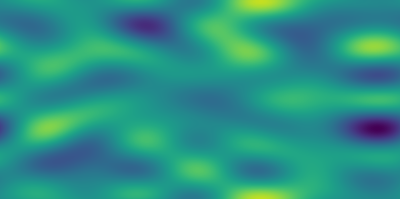
\includegraphics[interpolate=false,width=1.000000in,height=1.000000in]{burgers_rollout_target_0.0-img0.png}}%
\end{pgfscope}%
\begin{pgfscope}%
\pgfsetbuttcap%
\pgfsetroundjoin%
\definecolor{currentfill}{rgb}{0.000000,0.000000,0.000000}%
\pgfsetfillcolor{currentfill}%
\pgfsetlinewidth{0.803000pt}%
\definecolor{currentstroke}{rgb}{0.000000,0.000000,0.000000}%
\pgfsetstrokecolor{currentstroke}%
\pgfsetdash{}{0pt}%
\pgfsys@defobject{currentmarker}{\pgfqpoint{0.000000in}{-0.048611in}}{\pgfqpoint{0.000000in}{0.000000in}}{%
\pgfpathmoveto{\pgfqpoint{0.000000in}{0.000000in}}%
\pgfpathlineto{\pgfqpoint{0.000000in}{-0.048611in}}%
\pgfusepath{stroke,fill}%
}%
\begin{pgfscope}%
\pgfsys@transformshift{0.726837in}{0.517039in}%
\pgfsys@useobject{currentmarker}{}%
\end{pgfscope}%
\end{pgfscope}%
\begin{pgfscope}%
\definecolor{textcolor}{rgb}{0.000000,0.000000,0.000000}%
\pgfsetstrokecolor{textcolor}%
\pgfsetfillcolor{textcolor}%
\pgftext[x=0.726837in,y=0.419816in,,top]{\color{textcolor}{\rmfamily\fontsize{12.000000}{14.400000}\selectfont\catcode`\^=\active\def^{\ifmmode\sp\else\^{}\fi}\catcode`\%=\active\def%{\%}0}}%
\end{pgfscope}%
\begin{pgfscope}%
\pgfsetbuttcap%
\pgfsetroundjoin%
\definecolor{currentfill}{rgb}{0.000000,0.000000,0.000000}%
\pgfsetfillcolor{currentfill}%
\pgfsetlinewidth{0.803000pt}%
\definecolor{currentstroke}{rgb}{0.000000,0.000000,0.000000}%
\pgfsetstrokecolor{currentstroke}%
\pgfsetdash{}{0pt}%
\pgfsys@defobject{currentmarker}{\pgfqpoint{0.000000in}{-0.048611in}}{\pgfqpoint{0.000000in}{0.000000in}}{%
\pgfpathmoveto{\pgfqpoint{0.000000in}{0.000000in}}%
\pgfpathlineto{\pgfqpoint{0.000000in}{-0.048611in}}%
\pgfusepath{stroke,fill}%
}%
\begin{pgfscope}%
\pgfsys@transformshift{1.570762in}{0.517039in}%
\pgfsys@useobject{currentmarker}{}%
\end{pgfscope}%
\end{pgfscope}%
\begin{pgfscope}%
\definecolor{textcolor}{rgb}{0.000000,0.000000,0.000000}%
\pgfsetstrokecolor{textcolor}%
\pgfsetfillcolor{textcolor}%
\pgftext[x=1.570762in,y=0.419816in,,top]{\color{textcolor}{\rmfamily\fontsize{12.000000}{14.400000}\selectfont\catcode`\^=\active\def^{\ifmmode\sp\else\^{}\fi}\catcode`\%=\active\def%{\%}1}}%
\end{pgfscope}%
\begin{pgfscope}%
\pgfsetbuttcap%
\pgfsetroundjoin%
\definecolor{currentfill}{rgb}{0.000000,0.000000,0.000000}%
\pgfsetfillcolor{currentfill}%
\pgfsetlinewidth{0.803000pt}%
\definecolor{currentstroke}{rgb}{0.000000,0.000000,0.000000}%
\pgfsetstrokecolor{currentstroke}%
\pgfsetdash{}{0pt}%
\pgfsys@defobject{currentmarker}{\pgfqpoint{0.000000in}{-0.048611in}}{\pgfqpoint{0.000000in}{0.000000in}}{%
\pgfpathmoveto{\pgfqpoint{0.000000in}{0.000000in}}%
\pgfpathlineto{\pgfqpoint{0.000000in}{-0.048611in}}%
\pgfusepath{stroke,fill}%
}%
\begin{pgfscope}%
\pgfsys@transformshift{2.414687in}{0.517039in}%
\pgfsys@useobject{currentmarker}{}%
\end{pgfscope}%
\end{pgfscope}%
\begin{pgfscope}%
\definecolor{textcolor}{rgb}{0.000000,0.000000,0.000000}%
\pgfsetstrokecolor{textcolor}%
\pgfsetfillcolor{textcolor}%
\pgftext[x=2.414687in,y=0.419816in,,top]{\color{textcolor}{\rmfamily\fontsize{12.000000}{14.400000}\selectfont\catcode`\^=\active\def^{\ifmmode\sp\else\^{}\fi}\catcode`\%=\active\def%{\%}2}}%
\end{pgfscope}%
\begin{pgfscope}%
\definecolor{textcolor}{rgb}{0.000000,0.000000,0.000000}%
\pgfsetstrokecolor{textcolor}%
\pgfsetfillcolor{textcolor}%
\pgftext[x=1.570762in,y=0.202965in,,top]{\color{textcolor}{\rmfamily\fontsize{12.000000}{14.400000}\selectfont\catcode`\^=\active\def^{\ifmmode\sp\else\^{}\fi}\catcode`\%=\active\def%{\%}Space}}%
\end{pgfscope}%
\begin{pgfscope}%
\pgfsetbuttcap%
\pgfsetroundjoin%
\definecolor{currentfill}{rgb}{0.000000,0.000000,0.000000}%
\pgfsetfillcolor{currentfill}%
\pgfsetlinewidth{0.803000pt}%
\definecolor{currentstroke}{rgb}{0.000000,0.000000,0.000000}%
\pgfsetstrokecolor{currentstroke}%
\pgfsetdash{}{0pt}%
\pgfsys@defobject{currentmarker}{\pgfqpoint{-0.048611in}{0.000000in}}{\pgfqpoint{-0.000000in}{0.000000in}}{%
\pgfpathmoveto{\pgfqpoint{-0.000000in}{0.000000in}}%
\pgfpathlineto{\pgfqpoint{-0.048611in}{0.000000in}}%
\pgfusepath{stroke,fill}%
}%
\begin{pgfscope}%
\pgfsys@transformshift{0.726837in}{0.517039in}%
\pgfsys@useobject{currentmarker}{}%
\end{pgfscope}%
\end{pgfscope}%
\begin{pgfscope}%
\definecolor{textcolor}{rgb}{0.000000,0.000000,0.000000}%
\pgfsetstrokecolor{textcolor}%
\pgfsetfillcolor{textcolor}%
\pgftext[x=0.364559in, y=0.453725in, left, base]{\color{textcolor}{\rmfamily\fontsize{12.000000}{14.400000}\selectfont\catcode`\^=\active\def^{\ifmmode\sp\else\^{}\fi}\catcode`\%=\active\def%{\%}0.0}}%
\end{pgfscope}%
\begin{pgfscope}%
\pgfsetbuttcap%
\pgfsetroundjoin%
\definecolor{currentfill}{rgb}{0.000000,0.000000,0.000000}%
\pgfsetfillcolor{currentfill}%
\pgfsetlinewidth{0.803000pt}%
\definecolor{currentstroke}{rgb}{0.000000,0.000000,0.000000}%
\pgfsetstrokecolor{currentstroke}%
\pgfsetdash{}{0pt}%
\pgfsys@defobject{currentmarker}{\pgfqpoint{-0.048611in}{0.000000in}}{\pgfqpoint{-0.000000in}{0.000000in}}{%
\pgfpathmoveto{\pgfqpoint{-0.000000in}{0.000000in}}%
\pgfpathlineto{\pgfqpoint{-0.048611in}{0.000000in}}%
\pgfusepath{stroke,fill}%
}%
\begin{pgfscope}%
\pgfsys@transformshift{0.726837in}{0.861533in}%
\pgfsys@useobject{currentmarker}{}%
\end{pgfscope}%
\end{pgfscope}%
\begin{pgfscope}%
\definecolor{textcolor}{rgb}{0.000000,0.000000,0.000000}%
\pgfsetstrokecolor{textcolor}%
\pgfsetfillcolor{textcolor}%
\pgftext[x=0.364559in, y=0.798219in, left, base]{\color{textcolor}{\rmfamily\fontsize{12.000000}{14.400000}\selectfont\catcode`\^=\active\def^{\ifmmode\sp\else\^{}\fi}\catcode`\%=\active\def%{\%}2.5}}%
\end{pgfscope}%
\begin{pgfscope}%
\pgfsetbuttcap%
\pgfsetroundjoin%
\definecolor{currentfill}{rgb}{0.000000,0.000000,0.000000}%
\pgfsetfillcolor{currentfill}%
\pgfsetlinewidth{0.803000pt}%
\definecolor{currentstroke}{rgb}{0.000000,0.000000,0.000000}%
\pgfsetstrokecolor{currentstroke}%
\pgfsetdash{}{0pt}%
\pgfsys@defobject{currentmarker}{\pgfqpoint{-0.048611in}{0.000000in}}{\pgfqpoint{-0.000000in}{0.000000in}}{%
\pgfpathmoveto{\pgfqpoint{-0.000000in}{0.000000in}}%
\pgfpathlineto{\pgfqpoint{-0.048611in}{0.000000in}}%
\pgfusepath{stroke,fill}%
}%
\begin{pgfscope}%
\pgfsys@transformshift{0.726837in}{1.206027in}%
\pgfsys@useobject{currentmarker}{}%
\end{pgfscope}%
\end{pgfscope}%
\begin{pgfscope}%
\definecolor{textcolor}{rgb}{0.000000,0.000000,0.000000}%
\pgfsetstrokecolor{textcolor}%
\pgfsetfillcolor{textcolor}%
\pgftext[x=0.364559in, y=1.142714in, left, base]{\color{textcolor}{\rmfamily\fontsize{12.000000}{14.400000}\selectfont\catcode`\^=\active\def^{\ifmmode\sp\else\^{}\fi}\catcode`\%=\active\def%{\%}5.0}}%
\end{pgfscope}%
\begin{pgfscope}%
\pgfsetbuttcap%
\pgfsetroundjoin%
\definecolor{currentfill}{rgb}{0.000000,0.000000,0.000000}%
\pgfsetfillcolor{currentfill}%
\pgfsetlinewidth{0.803000pt}%
\definecolor{currentstroke}{rgb}{0.000000,0.000000,0.000000}%
\pgfsetstrokecolor{currentstroke}%
\pgfsetdash{}{0pt}%
\pgfsys@defobject{currentmarker}{\pgfqpoint{-0.048611in}{0.000000in}}{\pgfqpoint{-0.000000in}{0.000000in}}{%
\pgfpathmoveto{\pgfqpoint{-0.000000in}{0.000000in}}%
\pgfpathlineto{\pgfqpoint{-0.048611in}{0.000000in}}%
\pgfusepath{stroke,fill}%
}%
\begin{pgfscope}%
\pgfsys@transformshift{0.726837in}{1.550522in}%
\pgfsys@useobject{currentmarker}{}%
\end{pgfscope}%
\end{pgfscope}%
\begin{pgfscope}%
\definecolor{textcolor}{rgb}{0.000000,0.000000,0.000000}%
\pgfsetstrokecolor{textcolor}%
\pgfsetfillcolor{textcolor}%
\pgftext[x=0.364559in, y=1.487208in, left, base]{\color{textcolor}{\rmfamily\fontsize{12.000000}{14.400000}\selectfont\catcode`\^=\active\def^{\ifmmode\sp\else\^{}\fi}\catcode`\%=\active\def%{\%}7.5}}%
\end{pgfscope}%
\begin{pgfscope}%
\pgfsetbuttcap%
\pgfsetroundjoin%
\definecolor{currentfill}{rgb}{0.000000,0.000000,0.000000}%
\pgfsetfillcolor{currentfill}%
\pgfsetlinewidth{0.803000pt}%
\definecolor{currentstroke}{rgb}{0.000000,0.000000,0.000000}%
\pgfsetstrokecolor{currentstroke}%
\pgfsetdash{}{0pt}%
\pgfsys@defobject{currentmarker}{\pgfqpoint{-0.048611in}{0.000000in}}{\pgfqpoint{-0.000000in}{0.000000in}}{%
\pgfpathmoveto{\pgfqpoint{-0.000000in}{0.000000in}}%
\pgfpathlineto{\pgfqpoint{-0.048611in}{0.000000in}}%
\pgfusepath{stroke,fill}%
}%
\begin{pgfscope}%
\pgfsys@transformshift{0.726837in}{1.895016in}%
\pgfsys@useobject{currentmarker}{}%
\end{pgfscope}%
\end{pgfscope}%
\begin{pgfscope}%
\definecolor{textcolor}{rgb}{0.000000,0.000000,0.000000}%
\pgfsetstrokecolor{textcolor}%
\pgfsetfillcolor{textcolor}%
\pgftext[x=0.258521in, y=1.831702in, left, base]{\color{textcolor}{\rmfamily\fontsize{12.000000}{14.400000}\selectfont\catcode`\^=\active\def^{\ifmmode\sp\else\^{}\fi}\catcode`\%=\active\def%{\%}10.0}}%
\end{pgfscope}%
\begin{pgfscope}%
\definecolor{textcolor}{rgb}{0.000000,0.000000,0.000000}%
\pgfsetstrokecolor{textcolor}%
\pgfsetfillcolor{textcolor}%
\pgftext[x=0.202965in,y=1.206027in,,bottom,rotate=90.000000]{\color{textcolor}{\rmfamily\fontsize{12.000000}{14.400000}\selectfont\catcode`\^=\active\def^{\ifmmode\sp\else\^{}\fi}\catcode`\%=\active\def%{\%}Time}}%
\end{pgfscope}%
\begin{pgfscope}%
\pgfsetrectcap%
\pgfsetmiterjoin%
\pgfsetlinewidth{0.803000pt}%
\definecolor{currentstroke}{rgb}{0.000000,0.000000,0.000000}%
\pgfsetstrokecolor{currentstroke}%
\pgfsetdash{}{0pt}%
\pgfpathmoveto{\pgfqpoint{0.726837in}{0.517039in}}%
\pgfpathlineto{\pgfqpoint{0.726837in}{1.895016in}}%
\pgfusepath{stroke}%
\end{pgfscope}%
\begin{pgfscope}%
\pgfsetrectcap%
\pgfsetmiterjoin%
\pgfsetlinewidth{0.803000pt}%
\definecolor{currentstroke}{rgb}{0.000000,0.000000,0.000000}%
\pgfsetstrokecolor{currentstroke}%
\pgfsetdash{}{0pt}%
\pgfpathmoveto{\pgfqpoint{2.414687in}{0.517039in}}%
\pgfpathlineto{\pgfqpoint{2.414687in}{1.895016in}}%
\pgfusepath{stroke}%
\end{pgfscope}%
\begin{pgfscope}%
\pgfsetrectcap%
\pgfsetmiterjoin%
\pgfsetlinewidth{0.803000pt}%
\definecolor{currentstroke}{rgb}{0.000000,0.000000,0.000000}%
\pgfsetstrokecolor{currentstroke}%
\pgfsetdash{}{0pt}%
\pgfpathmoveto{\pgfqpoint{0.726837in}{0.517039in}}%
\pgfpathlineto{\pgfqpoint{2.414687in}{0.517039in}}%
\pgfusepath{stroke}%
\end{pgfscope}%
\begin{pgfscope}%
\pgfsetrectcap%
\pgfsetmiterjoin%
\pgfsetlinewidth{0.803000pt}%
\definecolor{currentstroke}{rgb}{0.000000,0.000000,0.000000}%
\pgfsetstrokecolor{currentstroke}%
\pgfsetdash{}{0pt}%
\pgfpathmoveto{\pgfqpoint{0.726837in}{1.895016in}}%
\pgfpathlineto{\pgfqpoint{2.414687in}{1.895016in}}%
\pgfusepath{stroke}%
\end{pgfscope}%
\begin{pgfscope}%
\pgfsetbuttcap%
\pgfsetmiterjoin%
\pgfsetlinewidth{0.000000pt}%
\definecolor{currentstroke}{rgb}{0.000000,0.000000,0.000000}%
\pgfsetstrokecolor{currentstroke}%
\pgfsetstrokeopacity{0.000000}%
\pgfsetdash{}{0pt}%
\pgfpathmoveto{\pgfqpoint{2.552099in}{0.517039in}}%
\pgfpathlineto{\pgfqpoint{2.620998in}{0.517039in}}%
\pgfpathlineto{\pgfqpoint{2.620998in}{1.895016in}}%
\pgfpathlineto{\pgfqpoint{2.552099in}{1.895016in}}%
\pgfpathlineto{\pgfqpoint{2.552099in}{0.517039in}}%
\pgfpathclose%
\pgfusepath{}%
\end{pgfscope}%
\begin{pgfscope}%
\pgfsys@transformshift{2.550000in}{0.520000in}%
\pgftext[left,bottom]{
\includegraphics[interpolate=true,width=0.070000in,height=1.380000in]{burgers_rollout_target_0.0-img1.png}}%
\end{pgfscope}%
\begin{pgfscope}%
\pgfsetbuttcap%
\pgfsetroundjoin%
\definecolor{currentfill}{rgb}{0.000000,0.000000,0.000000}%
\pgfsetfillcolor{currentfill}%
\pgfsetlinewidth{0.803000pt}%
\definecolor{currentstroke}{rgb}{0.000000,0.000000,0.000000}%
\pgfsetstrokecolor{currentstroke}%
\pgfsetdash{}{0pt}%
\pgfsys@defobject{currentmarker}{\pgfqpoint{0.000000in}{0.000000in}}{\pgfqpoint{0.048611in}{0.000000in}}{%
\pgfpathmoveto{\pgfqpoint{0.000000in}{0.000000in}}%
\pgfpathlineto{\pgfqpoint{0.048611in}{0.000000in}}%
\pgfusepath{stroke,fill}%
}%
\begin{pgfscope}%
\pgfsys@transformshift{2.620998in}{0.588723in}%
\pgfsys@useobject{currentmarker}{}%
\end{pgfscope}%
\end{pgfscope}%
\begin{pgfscope}%
\definecolor{textcolor}{rgb}{0.000000,0.000000,0.000000}%
\pgfsetstrokecolor{textcolor}%
\pgfsetfillcolor{textcolor}%
\pgftext[x=2.718220in, y=0.525410in, left, base]{\color{textcolor}{\rmfamily\fontsize{12.000000}{14.400000}\selectfont\catcode`\^=\active\def^{\ifmmode\sp\else\^{}\fi}\catcode`\%=\active\def%{\%}\ensuremath{-}1}}%
\end{pgfscope}%
\begin{pgfscope}%
\pgfsetbuttcap%
\pgfsetroundjoin%
\definecolor{currentfill}{rgb}{0.000000,0.000000,0.000000}%
\pgfsetfillcolor{currentfill}%
\pgfsetlinewidth{0.803000pt}%
\definecolor{currentstroke}{rgb}{0.000000,0.000000,0.000000}%
\pgfsetstrokecolor{currentstroke}%
\pgfsetdash{}{0pt}%
\pgfsys@defobject{currentmarker}{\pgfqpoint{0.000000in}{0.000000in}}{\pgfqpoint{0.048611in}{0.000000in}}{%
\pgfpathmoveto{\pgfqpoint{0.000000in}{0.000000in}}%
\pgfpathlineto{\pgfqpoint{0.048611in}{0.000000in}}%
\pgfusepath{stroke,fill}%
}%
\begin{pgfscope}%
\pgfsys@transformshift{2.620998in}{1.206027in}%
\pgfsys@useobject{currentmarker}{}%
\end{pgfscope}%
\end{pgfscope}%
\begin{pgfscope}%
\definecolor{textcolor}{rgb}{0.000000,0.000000,0.000000}%
\pgfsetstrokecolor{textcolor}%
\pgfsetfillcolor{textcolor}%
\pgftext[x=2.718220in, y=1.142714in, left, base]{\color{textcolor}{\rmfamily\fontsize{12.000000}{14.400000}\selectfont\catcode`\^=\active\def^{\ifmmode\sp\else\^{}\fi}\catcode`\%=\active\def%{\%}0}}%
\end{pgfscope}%
\begin{pgfscope}%
\pgfsetbuttcap%
\pgfsetroundjoin%
\definecolor{currentfill}{rgb}{0.000000,0.000000,0.000000}%
\pgfsetfillcolor{currentfill}%
\pgfsetlinewidth{0.803000pt}%
\definecolor{currentstroke}{rgb}{0.000000,0.000000,0.000000}%
\pgfsetstrokecolor{currentstroke}%
\pgfsetdash{}{0pt}%
\pgfsys@defobject{currentmarker}{\pgfqpoint{0.000000in}{0.000000in}}{\pgfqpoint{0.048611in}{0.000000in}}{%
\pgfpathmoveto{\pgfqpoint{0.000000in}{0.000000in}}%
\pgfpathlineto{\pgfqpoint{0.048611in}{0.000000in}}%
\pgfusepath{stroke,fill}%
}%
\begin{pgfscope}%
\pgfsys@transformshift{2.620998in}{1.823331in}%
\pgfsys@useobject{currentmarker}{}%
\end{pgfscope}%
\end{pgfscope}%
\begin{pgfscope}%
\definecolor{textcolor}{rgb}{0.000000,0.000000,0.000000}%
\pgfsetstrokecolor{textcolor}%
\pgfsetfillcolor{textcolor}%
\pgftext[x=2.718220in, y=1.760018in, left, base]{\color{textcolor}{\rmfamily\fontsize{12.000000}{14.400000}\selectfont\catcode`\^=\active\def^{\ifmmode\sp\else\^{}\fi}\catcode`\%=\active\def%{\%}1}}%
\end{pgfscope}%
\begin{pgfscope}%
\pgfsetrectcap%
\pgfsetmiterjoin%
\pgfsetlinewidth{0.803000pt}%
\definecolor{currentstroke}{rgb}{0.000000,0.000000,0.000000}%
\pgfsetstrokecolor{currentstroke}%
\pgfsetdash{}{0pt}%
\pgfpathmoveto{\pgfqpoint{2.552099in}{0.517039in}}%
\pgfpathlineto{\pgfqpoint{2.586548in}{0.517039in}}%
\pgfpathlineto{\pgfqpoint{2.620998in}{0.517039in}}%
\pgfpathlineto{\pgfqpoint{2.620998in}{1.895016in}}%
\pgfpathlineto{\pgfqpoint{2.586548in}{1.895016in}}%
\pgfpathlineto{\pgfqpoint{2.552099in}{1.895016in}}%
\pgfpathlineto{\pgfqpoint{2.552099in}{0.517039in}}%
\pgfpathclose%
\pgfusepath{stroke}%
\end{pgfscope}%
\end{pgfpicture}%
\makeatother%
\endgroup%

      \end{adjustbox}
      \caption{The target for \(\nu=0.0\)}\label{fig:sc2_rollout_target_0.0}
    \end{subfigure}
    \begin{subfigure}{0.33\linewidth}
      \begin{adjustbox}{width=\linewidth}
        \begingroup%
\makeatletter%
\begin{pgfpicture}%
\pgfpathrectangle{\pgfpointorigin}{\pgfqpoint{3.000000in}{2.000000in}}%
\pgfusepath{use as bounding box, clip}%
\begin{pgfscope}%
\pgfsetbuttcap%
\pgfsetmiterjoin%
\pgfsetlinewidth{0.000000pt}%
\definecolor{currentstroke}{rgb}{0.000000,0.000000,0.000000}%
\pgfsetstrokecolor{currentstroke}%
\pgfsetstrokeopacity{0.000000}%
\pgfsetdash{}{0pt}%
\pgfpathmoveto{\pgfqpoint{0.000000in}{0.000000in}}%
\pgfpathlineto{\pgfqpoint{3.000000in}{0.000000in}}%
\pgfpathlineto{\pgfqpoint{3.000000in}{2.000000in}}%
\pgfpathlineto{\pgfqpoint{0.000000in}{2.000000in}}%
\pgfpathlineto{\pgfqpoint{0.000000in}{0.000000in}}%
\pgfpathclose%
\pgfusepath{}%
\end{pgfscope}%
\begin{pgfscope}%
\pgfsetbuttcap%
\pgfsetmiterjoin%
\pgfsetlinewidth{0.000000pt}%
\definecolor{currentstroke}{rgb}{0.000000,0.000000,0.000000}%
\pgfsetstrokecolor{currentstroke}%
\pgfsetstrokeopacity{0.000000}%
\pgfsetdash{}{0pt}%
\pgfpathmoveto{\pgfqpoint{0.726837in}{0.517039in}}%
\pgfpathlineto{\pgfqpoint{2.414687in}{0.517039in}}%
\pgfpathlineto{\pgfqpoint{2.414687in}{1.895016in}}%
\pgfpathlineto{\pgfqpoint{0.726837in}{1.895016in}}%
\pgfpathlineto{\pgfqpoint{0.726837in}{0.517039in}}%
\pgfpathclose%
\pgfusepath{}%
\end{pgfscope}%
\begin{pgfscope}%
\pgfpathrectangle{\pgfqpoint{0.726837in}{0.517039in}}{\pgfqpoint{1.687850in}{1.377978in}}%
\pgfusepath{clip}%
\pgfsys@transformcm{1.687850}{0.000000}{0.000000}{1.377978}{0.726837in}{0.517039in}%
\pgftext[left,bottom]{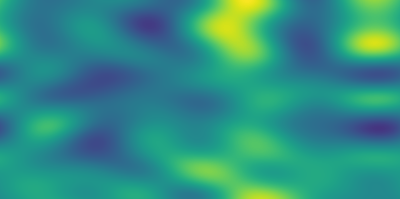
\includegraphics[interpolate=false,width=1.000000in,height=1.000000in]{burgers_rollout_pred_0.0-img0.png}}%
\end{pgfscope}%
\begin{pgfscope}%
\pgfsetbuttcap%
\pgfsetroundjoin%
\definecolor{currentfill}{rgb}{0.000000,0.000000,0.000000}%
\pgfsetfillcolor{currentfill}%
\pgfsetlinewidth{0.803000pt}%
\definecolor{currentstroke}{rgb}{0.000000,0.000000,0.000000}%
\pgfsetstrokecolor{currentstroke}%
\pgfsetdash{}{0pt}%
\pgfsys@defobject{currentmarker}{\pgfqpoint{0.000000in}{-0.048611in}}{\pgfqpoint{0.000000in}{0.000000in}}{%
\pgfpathmoveto{\pgfqpoint{0.000000in}{0.000000in}}%
\pgfpathlineto{\pgfqpoint{0.000000in}{-0.048611in}}%
\pgfusepath{stroke,fill}%
}%
\begin{pgfscope}%
\pgfsys@transformshift{0.726837in}{0.517039in}%
\pgfsys@useobject{currentmarker}{}%
\end{pgfscope}%
\end{pgfscope}%
\begin{pgfscope}%
\definecolor{textcolor}{rgb}{0.000000,0.000000,0.000000}%
\pgfsetstrokecolor{textcolor}%
\pgfsetfillcolor{textcolor}%
\pgftext[x=0.726837in,y=0.419816in,,top]{\color{textcolor}{\rmfamily\fontsize{12.000000}{14.400000}\selectfont\catcode`\^=\active\def^{\ifmmode\sp\else\^{}\fi}\catcode`\%=\active\def%{\%}0}}%
\end{pgfscope}%
\begin{pgfscope}%
\pgfsetbuttcap%
\pgfsetroundjoin%
\definecolor{currentfill}{rgb}{0.000000,0.000000,0.000000}%
\pgfsetfillcolor{currentfill}%
\pgfsetlinewidth{0.803000pt}%
\definecolor{currentstroke}{rgb}{0.000000,0.000000,0.000000}%
\pgfsetstrokecolor{currentstroke}%
\pgfsetdash{}{0pt}%
\pgfsys@defobject{currentmarker}{\pgfqpoint{0.000000in}{-0.048611in}}{\pgfqpoint{0.000000in}{0.000000in}}{%
\pgfpathmoveto{\pgfqpoint{0.000000in}{0.000000in}}%
\pgfpathlineto{\pgfqpoint{0.000000in}{-0.048611in}}%
\pgfusepath{stroke,fill}%
}%
\begin{pgfscope}%
\pgfsys@transformshift{1.570762in}{0.517039in}%
\pgfsys@useobject{currentmarker}{}%
\end{pgfscope}%
\end{pgfscope}%
\begin{pgfscope}%
\definecolor{textcolor}{rgb}{0.000000,0.000000,0.000000}%
\pgfsetstrokecolor{textcolor}%
\pgfsetfillcolor{textcolor}%
\pgftext[x=1.570762in,y=0.419816in,,top]{\color{textcolor}{\rmfamily\fontsize{12.000000}{14.400000}\selectfont\catcode`\^=\active\def^{\ifmmode\sp\else\^{}\fi}\catcode`\%=\active\def%{\%}1}}%
\end{pgfscope}%
\begin{pgfscope}%
\pgfsetbuttcap%
\pgfsetroundjoin%
\definecolor{currentfill}{rgb}{0.000000,0.000000,0.000000}%
\pgfsetfillcolor{currentfill}%
\pgfsetlinewidth{0.803000pt}%
\definecolor{currentstroke}{rgb}{0.000000,0.000000,0.000000}%
\pgfsetstrokecolor{currentstroke}%
\pgfsetdash{}{0pt}%
\pgfsys@defobject{currentmarker}{\pgfqpoint{0.000000in}{-0.048611in}}{\pgfqpoint{0.000000in}{0.000000in}}{%
\pgfpathmoveto{\pgfqpoint{0.000000in}{0.000000in}}%
\pgfpathlineto{\pgfqpoint{0.000000in}{-0.048611in}}%
\pgfusepath{stroke,fill}%
}%
\begin{pgfscope}%
\pgfsys@transformshift{2.414687in}{0.517039in}%
\pgfsys@useobject{currentmarker}{}%
\end{pgfscope}%
\end{pgfscope}%
\begin{pgfscope}%
\definecolor{textcolor}{rgb}{0.000000,0.000000,0.000000}%
\pgfsetstrokecolor{textcolor}%
\pgfsetfillcolor{textcolor}%
\pgftext[x=2.414687in,y=0.419816in,,top]{\color{textcolor}{\rmfamily\fontsize{12.000000}{14.400000}\selectfont\catcode`\^=\active\def^{\ifmmode\sp\else\^{}\fi}\catcode`\%=\active\def%{\%}2}}%
\end{pgfscope}%
\begin{pgfscope}%
\definecolor{textcolor}{rgb}{0.000000,0.000000,0.000000}%
\pgfsetstrokecolor{textcolor}%
\pgfsetfillcolor{textcolor}%
\pgftext[x=1.570762in,y=0.202965in,,top]{\color{textcolor}{\rmfamily\fontsize{12.000000}{14.400000}\selectfont\catcode`\^=\active\def^{\ifmmode\sp\else\^{}\fi}\catcode`\%=\active\def%{\%}Space}}%
\end{pgfscope}%
\begin{pgfscope}%
\pgfsetbuttcap%
\pgfsetroundjoin%
\definecolor{currentfill}{rgb}{0.000000,0.000000,0.000000}%
\pgfsetfillcolor{currentfill}%
\pgfsetlinewidth{0.803000pt}%
\definecolor{currentstroke}{rgb}{0.000000,0.000000,0.000000}%
\pgfsetstrokecolor{currentstroke}%
\pgfsetdash{}{0pt}%
\pgfsys@defobject{currentmarker}{\pgfqpoint{-0.048611in}{0.000000in}}{\pgfqpoint{-0.000000in}{0.000000in}}{%
\pgfpathmoveto{\pgfqpoint{-0.000000in}{0.000000in}}%
\pgfpathlineto{\pgfqpoint{-0.048611in}{0.000000in}}%
\pgfusepath{stroke,fill}%
}%
\begin{pgfscope}%
\pgfsys@transformshift{0.726837in}{0.517039in}%
\pgfsys@useobject{currentmarker}{}%
\end{pgfscope}%
\end{pgfscope}%
\begin{pgfscope}%
\definecolor{textcolor}{rgb}{0.000000,0.000000,0.000000}%
\pgfsetstrokecolor{textcolor}%
\pgfsetfillcolor{textcolor}%
\pgftext[x=0.364559in, y=0.453725in, left, base]{\color{textcolor}{\rmfamily\fontsize{12.000000}{14.400000}\selectfont\catcode`\^=\active\def^{\ifmmode\sp\else\^{}\fi}\catcode`\%=\active\def%{\%}0.0}}%
\end{pgfscope}%
\begin{pgfscope}%
\pgfsetbuttcap%
\pgfsetroundjoin%
\definecolor{currentfill}{rgb}{0.000000,0.000000,0.000000}%
\pgfsetfillcolor{currentfill}%
\pgfsetlinewidth{0.803000pt}%
\definecolor{currentstroke}{rgb}{0.000000,0.000000,0.000000}%
\pgfsetstrokecolor{currentstroke}%
\pgfsetdash{}{0pt}%
\pgfsys@defobject{currentmarker}{\pgfqpoint{-0.048611in}{0.000000in}}{\pgfqpoint{-0.000000in}{0.000000in}}{%
\pgfpathmoveto{\pgfqpoint{-0.000000in}{0.000000in}}%
\pgfpathlineto{\pgfqpoint{-0.048611in}{0.000000in}}%
\pgfusepath{stroke,fill}%
}%
\begin{pgfscope}%
\pgfsys@transformshift{0.726837in}{0.861533in}%
\pgfsys@useobject{currentmarker}{}%
\end{pgfscope}%
\end{pgfscope}%
\begin{pgfscope}%
\definecolor{textcolor}{rgb}{0.000000,0.000000,0.000000}%
\pgfsetstrokecolor{textcolor}%
\pgfsetfillcolor{textcolor}%
\pgftext[x=0.364559in, y=0.798219in, left, base]{\color{textcolor}{\rmfamily\fontsize{12.000000}{14.400000}\selectfont\catcode`\^=\active\def^{\ifmmode\sp\else\^{}\fi}\catcode`\%=\active\def%{\%}2.5}}%
\end{pgfscope}%
\begin{pgfscope}%
\pgfsetbuttcap%
\pgfsetroundjoin%
\definecolor{currentfill}{rgb}{0.000000,0.000000,0.000000}%
\pgfsetfillcolor{currentfill}%
\pgfsetlinewidth{0.803000pt}%
\definecolor{currentstroke}{rgb}{0.000000,0.000000,0.000000}%
\pgfsetstrokecolor{currentstroke}%
\pgfsetdash{}{0pt}%
\pgfsys@defobject{currentmarker}{\pgfqpoint{-0.048611in}{0.000000in}}{\pgfqpoint{-0.000000in}{0.000000in}}{%
\pgfpathmoveto{\pgfqpoint{-0.000000in}{0.000000in}}%
\pgfpathlineto{\pgfqpoint{-0.048611in}{0.000000in}}%
\pgfusepath{stroke,fill}%
}%
\begin{pgfscope}%
\pgfsys@transformshift{0.726837in}{1.206027in}%
\pgfsys@useobject{currentmarker}{}%
\end{pgfscope}%
\end{pgfscope}%
\begin{pgfscope}%
\definecolor{textcolor}{rgb}{0.000000,0.000000,0.000000}%
\pgfsetstrokecolor{textcolor}%
\pgfsetfillcolor{textcolor}%
\pgftext[x=0.364559in, y=1.142714in, left, base]{\color{textcolor}{\rmfamily\fontsize{12.000000}{14.400000}\selectfont\catcode`\^=\active\def^{\ifmmode\sp\else\^{}\fi}\catcode`\%=\active\def%{\%}5.0}}%
\end{pgfscope}%
\begin{pgfscope}%
\pgfsetbuttcap%
\pgfsetroundjoin%
\definecolor{currentfill}{rgb}{0.000000,0.000000,0.000000}%
\pgfsetfillcolor{currentfill}%
\pgfsetlinewidth{0.803000pt}%
\definecolor{currentstroke}{rgb}{0.000000,0.000000,0.000000}%
\pgfsetstrokecolor{currentstroke}%
\pgfsetdash{}{0pt}%
\pgfsys@defobject{currentmarker}{\pgfqpoint{-0.048611in}{0.000000in}}{\pgfqpoint{-0.000000in}{0.000000in}}{%
\pgfpathmoveto{\pgfqpoint{-0.000000in}{0.000000in}}%
\pgfpathlineto{\pgfqpoint{-0.048611in}{0.000000in}}%
\pgfusepath{stroke,fill}%
}%
\begin{pgfscope}%
\pgfsys@transformshift{0.726837in}{1.550522in}%
\pgfsys@useobject{currentmarker}{}%
\end{pgfscope}%
\end{pgfscope}%
\begin{pgfscope}%
\definecolor{textcolor}{rgb}{0.000000,0.000000,0.000000}%
\pgfsetstrokecolor{textcolor}%
\pgfsetfillcolor{textcolor}%
\pgftext[x=0.364559in, y=1.487208in, left, base]{\color{textcolor}{\rmfamily\fontsize{12.000000}{14.400000}\selectfont\catcode`\^=\active\def^{\ifmmode\sp\else\^{}\fi}\catcode`\%=\active\def%{\%}7.5}}%
\end{pgfscope}%
\begin{pgfscope}%
\pgfsetbuttcap%
\pgfsetroundjoin%
\definecolor{currentfill}{rgb}{0.000000,0.000000,0.000000}%
\pgfsetfillcolor{currentfill}%
\pgfsetlinewidth{0.803000pt}%
\definecolor{currentstroke}{rgb}{0.000000,0.000000,0.000000}%
\pgfsetstrokecolor{currentstroke}%
\pgfsetdash{}{0pt}%
\pgfsys@defobject{currentmarker}{\pgfqpoint{-0.048611in}{0.000000in}}{\pgfqpoint{-0.000000in}{0.000000in}}{%
\pgfpathmoveto{\pgfqpoint{-0.000000in}{0.000000in}}%
\pgfpathlineto{\pgfqpoint{-0.048611in}{0.000000in}}%
\pgfusepath{stroke,fill}%
}%
\begin{pgfscope}%
\pgfsys@transformshift{0.726837in}{1.895016in}%
\pgfsys@useobject{currentmarker}{}%
\end{pgfscope}%
\end{pgfscope}%
\begin{pgfscope}%
\definecolor{textcolor}{rgb}{0.000000,0.000000,0.000000}%
\pgfsetstrokecolor{textcolor}%
\pgfsetfillcolor{textcolor}%
\pgftext[x=0.258521in, y=1.831702in, left, base]{\color{textcolor}{\rmfamily\fontsize{12.000000}{14.400000}\selectfont\catcode`\^=\active\def^{\ifmmode\sp\else\^{}\fi}\catcode`\%=\active\def%{\%}10.0}}%
\end{pgfscope}%
\begin{pgfscope}%
\definecolor{textcolor}{rgb}{0.000000,0.000000,0.000000}%
\pgfsetstrokecolor{textcolor}%
\pgfsetfillcolor{textcolor}%
\pgftext[x=0.202965in,y=1.206027in,,bottom,rotate=90.000000]{\color{textcolor}{\rmfamily\fontsize{12.000000}{14.400000}\selectfont\catcode`\^=\active\def^{\ifmmode\sp\else\^{}\fi}\catcode`\%=\active\def%{\%}Time}}%
\end{pgfscope}%
\begin{pgfscope}%
\pgfsetrectcap%
\pgfsetmiterjoin%
\pgfsetlinewidth{0.803000pt}%
\definecolor{currentstroke}{rgb}{0.000000,0.000000,0.000000}%
\pgfsetstrokecolor{currentstroke}%
\pgfsetdash{}{0pt}%
\pgfpathmoveto{\pgfqpoint{0.726837in}{0.517039in}}%
\pgfpathlineto{\pgfqpoint{0.726837in}{1.895016in}}%
\pgfusepath{stroke}%
\end{pgfscope}%
\begin{pgfscope}%
\pgfsetrectcap%
\pgfsetmiterjoin%
\pgfsetlinewidth{0.803000pt}%
\definecolor{currentstroke}{rgb}{0.000000,0.000000,0.000000}%
\pgfsetstrokecolor{currentstroke}%
\pgfsetdash{}{0pt}%
\pgfpathmoveto{\pgfqpoint{2.414687in}{0.517039in}}%
\pgfpathlineto{\pgfqpoint{2.414687in}{1.895016in}}%
\pgfusepath{stroke}%
\end{pgfscope}%
\begin{pgfscope}%
\pgfsetrectcap%
\pgfsetmiterjoin%
\pgfsetlinewidth{0.803000pt}%
\definecolor{currentstroke}{rgb}{0.000000,0.000000,0.000000}%
\pgfsetstrokecolor{currentstroke}%
\pgfsetdash{}{0pt}%
\pgfpathmoveto{\pgfqpoint{0.726837in}{0.517039in}}%
\pgfpathlineto{\pgfqpoint{2.414687in}{0.517039in}}%
\pgfusepath{stroke}%
\end{pgfscope}%
\begin{pgfscope}%
\pgfsetrectcap%
\pgfsetmiterjoin%
\pgfsetlinewidth{0.803000pt}%
\definecolor{currentstroke}{rgb}{0.000000,0.000000,0.000000}%
\pgfsetstrokecolor{currentstroke}%
\pgfsetdash{}{0pt}%
\pgfpathmoveto{\pgfqpoint{0.726837in}{1.895016in}}%
\pgfpathlineto{\pgfqpoint{2.414687in}{1.895016in}}%
\pgfusepath{stroke}%
\end{pgfscope}%
\begin{pgfscope}%
\pgfsetbuttcap%
\pgfsetmiterjoin%
\pgfsetlinewidth{0.000000pt}%
\definecolor{currentstroke}{rgb}{0.000000,0.000000,0.000000}%
\pgfsetstrokecolor{currentstroke}%
\pgfsetstrokeopacity{0.000000}%
\pgfsetdash{}{0pt}%
\pgfpathmoveto{\pgfqpoint{2.552099in}{0.517039in}}%
\pgfpathlineto{\pgfqpoint{2.620998in}{0.517039in}}%
\pgfpathlineto{\pgfqpoint{2.620998in}{1.895016in}}%
\pgfpathlineto{\pgfqpoint{2.552099in}{1.895016in}}%
\pgfpathlineto{\pgfqpoint{2.552099in}{0.517039in}}%
\pgfpathclose%
\pgfusepath{}%
\end{pgfscope}%
\begin{pgfscope}%
\pgfsys@transformshift{2.550000in}{0.520000in}%
\pgftext[left,bottom]{
\includegraphics[interpolate=true,width=0.070000in,height=1.380000in]{burgers_rollout_pred_0.0-img1.png}}%
\end{pgfscope}%
\begin{pgfscope}%
\pgfsetbuttcap%
\pgfsetroundjoin%
\definecolor{currentfill}{rgb}{0.000000,0.000000,0.000000}%
\pgfsetfillcolor{currentfill}%
\pgfsetlinewidth{0.803000pt}%
\definecolor{currentstroke}{rgb}{0.000000,0.000000,0.000000}%
\pgfsetstrokecolor{currentstroke}%
\pgfsetdash{}{0pt}%
\pgfsys@defobject{currentmarker}{\pgfqpoint{0.000000in}{0.000000in}}{\pgfqpoint{0.048611in}{0.000000in}}{%
\pgfpathmoveto{\pgfqpoint{0.000000in}{0.000000in}}%
\pgfpathlineto{\pgfqpoint{0.048611in}{0.000000in}}%
\pgfusepath{stroke,fill}%
}%
\begin{pgfscope}%
\pgfsys@transformshift{2.620998in}{0.588723in}%
\pgfsys@useobject{currentmarker}{}%
\end{pgfscope}%
\end{pgfscope}%
\begin{pgfscope}%
\definecolor{textcolor}{rgb}{0.000000,0.000000,0.000000}%
\pgfsetstrokecolor{textcolor}%
\pgfsetfillcolor{textcolor}%
\pgftext[x=2.718220in, y=0.525410in, left, base]{\color{textcolor}{\rmfamily\fontsize{12.000000}{14.400000}\selectfont\catcode`\^=\active\def^{\ifmmode\sp\else\^{}\fi}\catcode`\%=\active\def%{\%}\ensuremath{-}1}}%
\end{pgfscope}%
\begin{pgfscope}%
\pgfsetbuttcap%
\pgfsetroundjoin%
\definecolor{currentfill}{rgb}{0.000000,0.000000,0.000000}%
\pgfsetfillcolor{currentfill}%
\pgfsetlinewidth{0.803000pt}%
\definecolor{currentstroke}{rgb}{0.000000,0.000000,0.000000}%
\pgfsetstrokecolor{currentstroke}%
\pgfsetdash{}{0pt}%
\pgfsys@defobject{currentmarker}{\pgfqpoint{0.000000in}{0.000000in}}{\pgfqpoint{0.048611in}{0.000000in}}{%
\pgfpathmoveto{\pgfqpoint{0.000000in}{0.000000in}}%
\pgfpathlineto{\pgfqpoint{0.048611in}{0.000000in}}%
\pgfusepath{stroke,fill}%
}%
\begin{pgfscope}%
\pgfsys@transformshift{2.620998in}{1.206027in}%
\pgfsys@useobject{currentmarker}{}%
\end{pgfscope}%
\end{pgfscope}%
\begin{pgfscope}%
\definecolor{textcolor}{rgb}{0.000000,0.000000,0.000000}%
\pgfsetstrokecolor{textcolor}%
\pgfsetfillcolor{textcolor}%
\pgftext[x=2.718220in, y=1.142714in, left, base]{\color{textcolor}{\rmfamily\fontsize{12.000000}{14.400000}\selectfont\catcode`\^=\active\def^{\ifmmode\sp\else\^{}\fi}\catcode`\%=\active\def%{\%}0}}%
\end{pgfscope}%
\begin{pgfscope}%
\pgfsetbuttcap%
\pgfsetroundjoin%
\definecolor{currentfill}{rgb}{0.000000,0.000000,0.000000}%
\pgfsetfillcolor{currentfill}%
\pgfsetlinewidth{0.803000pt}%
\definecolor{currentstroke}{rgb}{0.000000,0.000000,0.000000}%
\pgfsetstrokecolor{currentstroke}%
\pgfsetdash{}{0pt}%
\pgfsys@defobject{currentmarker}{\pgfqpoint{0.000000in}{0.000000in}}{\pgfqpoint{0.048611in}{0.000000in}}{%
\pgfpathmoveto{\pgfqpoint{0.000000in}{0.000000in}}%
\pgfpathlineto{\pgfqpoint{0.048611in}{0.000000in}}%
\pgfusepath{stroke,fill}%
}%
\begin{pgfscope}%
\pgfsys@transformshift{2.620998in}{1.823331in}%
\pgfsys@useobject{currentmarker}{}%
\end{pgfscope}%
\end{pgfscope}%
\begin{pgfscope}%
\definecolor{textcolor}{rgb}{0.000000,0.000000,0.000000}%
\pgfsetstrokecolor{textcolor}%
\pgfsetfillcolor{textcolor}%
\pgftext[x=2.718220in, y=1.760018in, left, base]{\color{textcolor}{\rmfamily\fontsize{12.000000}{14.400000}\selectfont\catcode`\^=\active\def^{\ifmmode\sp\else\^{}\fi}\catcode`\%=\active\def%{\%}1}}%
\end{pgfscope}%
\begin{pgfscope}%
\pgfsetrectcap%
\pgfsetmiterjoin%
\pgfsetlinewidth{0.803000pt}%
\definecolor{currentstroke}{rgb}{0.000000,0.000000,0.000000}%
\pgfsetstrokecolor{currentstroke}%
\pgfsetdash{}{0pt}%
\pgfpathmoveto{\pgfqpoint{2.552099in}{0.517039in}}%
\pgfpathlineto{\pgfqpoint{2.586548in}{0.517039in}}%
\pgfpathlineto{\pgfqpoint{2.620998in}{0.517039in}}%
\pgfpathlineto{\pgfqpoint{2.620998in}{1.895016in}}%
\pgfpathlineto{\pgfqpoint{2.586548in}{1.895016in}}%
\pgfpathlineto{\pgfqpoint{2.552099in}{1.895016in}}%
\pgfpathlineto{\pgfqpoint{2.552099in}{0.517039in}}%
\pgfpathclose%
\pgfusepath{stroke}%
\end{pgfscope}%
\end{pgfpicture}%
\makeatother%
\endgroup%

      \end{adjustbox}
      \caption{The prediction for \(\nu=0.0\)}\label{fig:sc2_rollout_pred_0.0}
    \end{subfigure}
    \begin{subfigure}{0.32\linewidth}
      \begin{adjustbox}{width=\linewidth}
        \begingroup%
\makeatletter%
\begin{pgfpicture}%
\pgfpathrectangle{\pgfpointorigin}{\pgfqpoint{3.000000in}{2.000000in}}%
\pgfusepath{use as bounding box, clip}%
\begin{pgfscope}%
\pgfsetbuttcap%
\pgfsetmiterjoin%
\pgfsetlinewidth{0.000000pt}%
\definecolor{currentstroke}{rgb}{0.000000,0.000000,0.000000}%
\pgfsetstrokecolor{currentstroke}%
\pgfsetstrokeopacity{0.000000}%
\pgfsetdash{}{0pt}%
\pgfpathmoveto{\pgfqpoint{0.000000in}{0.000000in}}%
\pgfpathlineto{\pgfqpoint{3.000000in}{0.000000in}}%
\pgfpathlineto{\pgfqpoint{3.000000in}{2.000000in}}%
\pgfpathlineto{\pgfqpoint{0.000000in}{2.000000in}}%
\pgfpathlineto{\pgfqpoint{0.000000in}{0.000000in}}%
\pgfpathclose%
\pgfusepath{}%
\end{pgfscope}%
\begin{pgfscope}%
\pgfsetbuttcap%
\pgfsetmiterjoin%
\pgfsetlinewidth{0.000000pt}%
\definecolor{currentstroke}{rgb}{0.000000,0.000000,0.000000}%
\pgfsetstrokecolor{currentstroke}%
\pgfsetstrokeopacity{0.000000}%
\pgfsetdash{}{0pt}%
\pgfpathmoveto{\pgfqpoint{0.726837in}{0.517039in}}%
\pgfpathlineto{\pgfqpoint{2.414687in}{0.517039in}}%
\pgfpathlineto{\pgfqpoint{2.414687in}{1.895016in}}%
\pgfpathlineto{\pgfqpoint{0.726837in}{1.895016in}}%
\pgfpathlineto{\pgfqpoint{0.726837in}{0.517039in}}%
\pgfpathclose%
\pgfusepath{}%
\end{pgfscope}%
\begin{pgfscope}%
\pgfpathrectangle{\pgfqpoint{0.726837in}{0.517039in}}{\pgfqpoint{1.687850in}{1.377978in}}%
\pgfusepath{clip}%
\pgfsys@transformcm{1.687850}{0.000000}{0.000000}{1.377978}{0.726837in}{0.517039in}%
\pgftext[left,bottom]{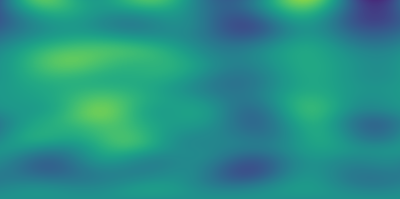
\includegraphics[interpolate=false,width=1.000000in,height=1.000000in]{burgers_rollout_diff_0.0-img0.png}}%
\end{pgfscope}%
\begin{pgfscope}%
\pgfsetbuttcap%
\pgfsetroundjoin%
\definecolor{currentfill}{rgb}{0.000000,0.000000,0.000000}%
\pgfsetfillcolor{currentfill}%
\pgfsetlinewidth{0.803000pt}%
\definecolor{currentstroke}{rgb}{0.000000,0.000000,0.000000}%
\pgfsetstrokecolor{currentstroke}%
\pgfsetdash{}{0pt}%
\pgfsys@defobject{currentmarker}{\pgfqpoint{0.000000in}{-0.048611in}}{\pgfqpoint{0.000000in}{0.000000in}}{%
\pgfpathmoveto{\pgfqpoint{0.000000in}{0.000000in}}%
\pgfpathlineto{\pgfqpoint{0.000000in}{-0.048611in}}%
\pgfusepath{stroke,fill}%
}%
\begin{pgfscope}%
\pgfsys@transformshift{0.726837in}{0.517039in}%
\pgfsys@useobject{currentmarker}{}%
\end{pgfscope}%
\end{pgfscope}%
\begin{pgfscope}%
\definecolor{textcolor}{rgb}{0.000000,0.000000,0.000000}%
\pgfsetstrokecolor{textcolor}%
\pgfsetfillcolor{textcolor}%
\pgftext[x=0.726837in,y=0.419816in,,top]{\color{textcolor}{\rmfamily\fontsize{12.000000}{14.400000}\selectfont\catcode`\^=\active\def^{\ifmmode\sp\else\^{}\fi}\catcode`\%=\active\def%{\%}0}}%
\end{pgfscope}%
\begin{pgfscope}%
\pgfsetbuttcap%
\pgfsetroundjoin%
\definecolor{currentfill}{rgb}{0.000000,0.000000,0.000000}%
\pgfsetfillcolor{currentfill}%
\pgfsetlinewidth{0.803000pt}%
\definecolor{currentstroke}{rgb}{0.000000,0.000000,0.000000}%
\pgfsetstrokecolor{currentstroke}%
\pgfsetdash{}{0pt}%
\pgfsys@defobject{currentmarker}{\pgfqpoint{0.000000in}{-0.048611in}}{\pgfqpoint{0.000000in}{0.000000in}}{%
\pgfpathmoveto{\pgfqpoint{0.000000in}{0.000000in}}%
\pgfpathlineto{\pgfqpoint{0.000000in}{-0.048611in}}%
\pgfusepath{stroke,fill}%
}%
\begin{pgfscope}%
\pgfsys@transformshift{1.570762in}{0.517039in}%
\pgfsys@useobject{currentmarker}{}%
\end{pgfscope}%
\end{pgfscope}%
\begin{pgfscope}%
\definecolor{textcolor}{rgb}{0.000000,0.000000,0.000000}%
\pgfsetstrokecolor{textcolor}%
\pgfsetfillcolor{textcolor}%
\pgftext[x=1.570762in,y=0.419816in,,top]{\color{textcolor}{\rmfamily\fontsize{12.000000}{14.400000}\selectfont\catcode`\^=\active\def^{\ifmmode\sp\else\^{}\fi}\catcode`\%=\active\def%{\%}1}}%
\end{pgfscope}%
\begin{pgfscope}%
\pgfsetbuttcap%
\pgfsetroundjoin%
\definecolor{currentfill}{rgb}{0.000000,0.000000,0.000000}%
\pgfsetfillcolor{currentfill}%
\pgfsetlinewidth{0.803000pt}%
\definecolor{currentstroke}{rgb}{0.000000,0.000000,0.000000}%
\pgfsetstrokecolor{currentstroke}%
\pgfsetdash{}{0pt}%
\pgfsys@defobject{currentmarker}{\pgfqpoint{0.000000in}{-0.048611in}}{\pgfqpoint{0.000000in}{0.000000in}}{%
\pgfpathmoveto{\pgfqpoint{0.000000in}{0.000000in}}%
\pgfpathlineto{\pgfqpoint{0.000000in}{-0.048611in}}%
\pgfusepath{stroke,fill}%
}%
\begin{pgfscope}%
\pgfsys@transformshift{2.414687in}{0.517039in}%
\pgfsys@useobject{currentmarker}{}%
\end{pgfscope}%
\end{pgfscope}%
\begin{pgfscope}%
\definecolor{textcolor}{rgb}{0.000000,0.000000,0.000000}%
\pgfsetstrokecolor{textcolor}%
\pgfsetfillcolor{textcolor}%
\pgftext[x=2.414687in,y=0.419816in,,top]{\color{textcolor}{\rmfamily\fontsize{12.000000}{14.400000}\selectfont\catcode`\^=\active\def^{\ifmmode\sp\else\^{}\fi}\catcode`\%=\active\def%{\%}2}}%
\end{pgfscope}%
\begin{pgfscope}%
\definecolor{textcolor}{rgb}{0.000000,0.000000,0.000000}%
\pgfsetstrokecolor{textcolor}%
\pgfsetfillcolor{textcolor}%
\pgftext[x=1.570762in,y=0.202965in,,top]{\color{textcolor}{\rmfamily\fontsize{12.000000}{14.400000}\selectfont\catcode`\^=\active\def^{\ifmmode\sp\else\^{}\fi}\catcode`\%=\active\def%{\%}Space}}%
\end{pgfscope}%
\begin{pgfscope}%
\pgfsetbuttcap%
\pgfsetroundjoin%
\definecolor{currentfill}{rgb}{0.000000,0.000000,0.000000}%
\pgfsetfillcolor{currentfill}%
\pgfsetlinewidth{0.803000pt}%
\definecolor{currentstroke}{rgb}{0.000000,0.000000,0.000000}%
\pgfsetstrokecolor{currentstroke}%
\pgfsetdash{}{0pt}%
\pgfsys@defobject{currentmarker}{\pgfqpoint{-0.048611in}{0.000000in}}{\pgfqpoint{-0.000000in}{0.000000in}}{%
\pgfpathmoveto{\pgfqpoint{-0.000000in}{0.000000in}}%
\pgfpathlineto{\pgfqpoint{-0.048611in}{0.000000in}}%
\pgfusepath{stroke,fill}%
}%
\begin{pgfscope}%
\pgfsys@transformshift{0.726837in}{0.517039in}%
\pgfsys@useobject{currentmarker}{}%
\end{pgfscope}%
\end{pgfscope}%
\begin{pgfscope}%
\definecolor{textcolor}{rgb}{0.000000,0.000000,0.000000}%
\pgfsetstrokecolor{textcolor}%
\pgfsetfillcolor{textcolor}%
\pgftext[x=0.364559in, y=0.453725in, left, base]{\color{textcolor}{\rmfamily\fontsize{12.000000}{14.400000}\selectfont\catcode`\^=\active\def^{\ifmmode\sp\else\^{}\fi}\catcode`\%=\active\def%{\%}0.0}}%
\end{pgfscope}%
\begin{pgfscope}%
\pgfsetbuttcap%
\pgfsetroundjoin%
\definecolor{currentfill}{rgb}{0.000000,0.000000,0.000000}%
\pgfsetfillcolor{currentfill}%
\pgfsetlinewidth{0.803000pt}%
\definecolor{currentstroke}{rgb}{0.000000,0.000000,0.000000}%
\pgfsetstrokecolor{currentstroke}%
\pgfsetdash{}{0pt}%
\pgfsys@defobject{currentmarker}{\pgfqpoint{-0.048611in}{0.000000in}}{\pgfqpoint{-0.000000in}{0.000000in}}{%
\pgfpathmoveto{\pgfqpoint{-0.000000in}{0.000000in}}%
\pgfpathlineto{\pgfqpoint{-0.048611in}{0.000000in}}%
\pgfusepath{stroke,fill}%
}%
\begin{pgfscope}%
\pgfsys@transformshift{0.726837in}{0.861533in}%
\pgfsys@useobject{currentmarker}{}%
\end{pgfscope}%
\end{pgfscope}%
\begin{pgfscope}%
\definecolor{textcolor}{rgb}{0.000000,0.000000,0.000000}%
\pgfsetstrokecolor{textcolor}%
\pgfsetfillcolor{textcolor}%
\pgftext[x=0.364559in, y=0.798219in, left, base]{\color{textcolor}{\rmfamily\fontsize{12.000000}{14.400000}\selectfont\catcode`\^=\active\def^{\ifmmode\sp\else\^{}\fi}\catcode`\%=\active\def%{\%}2.5}}%
\end{pgfscope}%
\begin{pgfscope}%
\pgfsetbuttcap%
\pgfsetroundjoin%
\definecolor{currentfill}{rgb}{0.000000,0.000000,0.000000}%
\pgfsetfillcolor{currentfill}%
\pgfsetlinewidth{0.803000pt}%
\definecolor{currentstroke}{rgb}{0.000000,0.000000,0.000000}%
\pgfsetstrokecolor{currentstroke}%
\pgfsetdash{}{0pt}%
\pgfsys@defobject{currentmarker}{\pgfqpoint{-0.048611in}{0.000000in}}{\pgfqpoint{-0.000000in}{0.000000in}}{%
\pgfpathmoveto{\pgfqpoint{-0.000000in}{0.000000in}}%
\pgfpathlineto{\pgfqpoint{-0.048611in}{0.000000in}}%
\pgfusepath{stroke,fill}%
}%
\begin{pgfscope}%
\pgfsys@transformshift{0.726837in}{1.206027in}%
\pgfsys@useobject{currentmarker}{}%
\end{pgfscope}%
\end{pgfscope}%
\begin{pgfscope}%
\definecolor{textcolor}{rgb}{0.000000,0.000000,0.000000}%
\pgfsetstrokecolor{textcolor}%
\pgfsetfillcolor{textcolor}%
\pgftext[x=0.364559in, y=1.142714in, left, base]{\color{textcolor}{\rmfamily\fontsize{12.000000}{14.400000}\selectfont\catcode`\^=\active\def^{\ifmmode\sp\else\^{}\fi}\catcode`\%=\active\def%{\%}5.0}}%
\end{pgfscope}%
\begin{pgfscope}%
\pgfsetbuttcap%
\pgfsetroundjoin%
\definecolor{currentfill}{rgb}{0.000000,0.000000,0.000000}%
\pgfsetfillcolor{currentfill}%
\pgfsetlinewidth{0.803000pt}%
\definecolor{currentstroke}{rgb}{0.000000,0.000000,0.000000}%
\pgfsetstrokecolor{currentstroke}%
\pgfsetdash{}{0pt}%
\pgfsys@defobject{currentmarker}{\pgfqpoint{-0.048611in}{0.000000in}}{\pgfqpoint{-0.000000in}{0.000000in}}{%
\pgfpathmoveto{\pgfqpoint{-0.000000in}{0.000000in}}%
\pgfpathlineto{\pgfqpoint{-0.048611in}{0.000000in}}%
\pgfusepath{stroke,fill}%
}%
\begin{pgfscope}%
\pgfsys@transformshift{0.726837in}{1.550522in}%
\pgfsys@useobject{currentmarker}{}%
\end{pgfscope}%
\end{pgfscope}%
\begin{pgfscope}%
\definecolor{textcolor}{rgb}{0.000000,0.000000,0.000000}%
\pgfsetstrokecolor{textcolor}%
\pgfsetfillcolor{textcolor}%
\pgftext[x=0.364559in, y=1.487208in, left, base]{\color{textcolor}{\rmfamily\fontsize{12.000000}{14.400000}\selectfont\catcode`\^=\active\def^{\ifmmode\sp\else\^{}\fi}\catcode`\%=\active\def%{\%}7.5}}%
\end{pgfscope}%
\begin{pgfscope}%
\pgfsetbuttcap%
\pgfsetroundjoin%
\definecolor{currentfill}{rgb}{0.000000,0.000000,0.000000}%
\pgfsetfillcolor{currentfill}%
\pgfsetlinewidth{0.803000pt}%
\definecolor{currentstroke}{rgb}{0.000000,0.000000,0.000000}%
\pgfsetstrokecolor{currentstroke}%
\pgfsetdash{}{0pt}%
\pgfsys@defobject{currentmarker}{\pgfqpoint{-0.048611in}{0.000000in}}{\pgfqpoint{-0.000000in}{0.000000in}}{%
\pgfpathmoveto{\pgfqpoint{-0.000000in}{0.000000in}}%
\pgfpathlineto{\pgfqpoint{-0.048611in}{0.000000in}}%
\pgfusepath{stroke,fill}%
}%
\begin{pgfscope}%
\pgfsys@transformshift{0.726837in}{1.895016in}%
\pgfsys@useobject{currentmarker}{}%
\end{pgfscope}%
\end{pgfscope}%
\begin{pgfscope}%
\definecolor{textcolor}{rgb}{0.000000,0.000000,0.000000}%
\pgfsetstrokecolor{textcolor}%
\pgfsetfillcolor{textcolor}%
\pgftext[x=0.258521in, y=1.831702in, left, base]{\color{textcolor}{\rmfamily\fontsize{12.000000}{14.400000}\selectfont\catcode`\^=\active\def^{\ifmmode\sp\else\^{}\fi}\catcode`\%=\active\def%{\%}10.0}}%
\end{pgfscope}%
\begin{pgfscope}%
\definecolor{textcolor}{rgb}{0.000000,0.000000,0.000000}%
\pgfsetstrokecolor{textcolor}%
\pgfsetfillcolor{textcolor}%
\pgftext[x=0.202965in,y=1.206027in,,bottom,rotate=90.000000]{\color{textcolor}{\rmfamily\fontsize{12.000000}{14.400000}\selectfont\catcode`\^=\active\def^{\ifmmode\sp\else\^{}\fi}\catcode`\%=\active\def%{\%}Time}}%
\end{pgfscope}%
\begin{pgfscope}%
\pgfsetrectcap%
\pgfsetmiterjoin%
\pgfsetlinewidth{0.803000pt}%
\definecolor{currentstroke}{rgb}{0.000000,0.000000,0.000000}%
\pgfsetstrokecolor{currentstroke}%
\pgfsetdash{}{0pt}%
\pgfpathmoveto{\pgfqpoint{0.726837in}{0.517039in}}%
\pgfpathlineto{\pgfqpoint{0.726837in}{1.895016in}}%
\pgfusepath{stroke}%
\end{pgfscope}%
\begin{pgfscope}%
\pgfsetrectcap%
\pgfsetmiterjoin%
\pgfsetlinewidth{0.803000pt}%
\definecolor{currentstroke}{rgb}{0.000000,0.000000,0.000000}%
\pgfsetstrokecolor{currentstroke}%
\pgfsetdash{}{0pt}%
\pgfpathmoveto{\pgfqpoint{2.414687in}{0.517039in}}%
\pgfpathlineto{\pgfqpoint{2.414687in}{1.895016in}}%
\pgfusepath{stroke}%
\end{pgfscope}%
\begin{pgfscope}%
\pgfsetrectcap%
\pgfsetmiterjoin%
\pgfsetlinewidth{0.803000pt}%
\definecolor{currentstroke}{rgb}{0.000000,0.000000,0.000000}%
\pgfsetstrokecolor{currentstroke}%
\pgfsetdash{}{0pt}%
\pgfpathmoveto{\pgfqpoint{0.726837in}{0.517039in}}%
\pgfpathlineto{\pgfqpoint{2.414687in}{0.517039in}}%
\pgfusepath{stroke}%
\end{pgfscope}%
\begin{pgfscope}%
\pgfsetrectcap%
\pgfsetmiterjoin%
\pgfsetlinewidth{0.803000pt}%
\definecolor{currentstroke}{rgb}{0.000000,0.000000,0.000000}%
\pgfsetstrokecolor{currentstroke}%
\pgfsetdash{}{0pt}%
\pgfpathmoveto{\pgfqpoint{0.726837in}{1.895016in}}%
\pgfpathlineto{\pgfqpoint{2.414687in}{1.895016in}}%
\pgfusepath{stroke}%
\end{pgfscope}%
\begin{pgfscope}%
\pgfsetbuttcap%
\pgfsetmiterjoin%
\pgfsetlinewidth{0.000000pt}%
\definecolor{currentstroke}{rgb}{0.000000,0.000000,0.000000}%
\pgfsetstrokecolor{currentstroke}%
\pgfsetstrokeopacity{0.000000}%
\pgfsetdash{}{0pt}%
\pgfpathmoveto{\pgfqpoint{2.552099in}{0.517039in}}%
\pgfpathlineto{\pgfqpoint{2.620998in}{0.517039in}}%
\pgfpathlineto{\pgfqpoint{2.620998in}{1.895016in}}%
\pgfpathlineto{\pgfqpoint{2.552099in}{1.895016in}}%
\pgfpathlineto{\pgfqpoint{2.552099in}{0.517039in}}%
\pgfpathclose%
\pgfusepath{}%
\end{pgfscope}%
\begin{pgfscope}%
\pgfsys@transformshift{2.550000in}{0.520000in}%
\pgftext[left,bottom]{
\includegraphics[interpolate=true,width=0.070000in,height=1.380000in]{burgers_rollout_diff_0.0-img1.png}}%
\end{pgfscope}%
\begin{pgfscope}%
\pgfsetbuttcap%
\pgfsetroundjoin%
\definecolor{currentfill}{rgb}{0.000000,0.000000,0.000000}%
\pgfsetfillcolor{currentfill}%
\pgfsetlinewidth{0.803000pt}%
\definecolor{currentstroke}{rgb}{0.000000,0.000000,0.000000}%
\pgfsetstrokecolor{currentstroke}%
\pgfsetdash{}{0pt}%
\pgfsys@defobject{currentmarker}{\pgfqpoint{0.000000in}{0.000000in}}{\pgfqpoint{0.048611in}{0.000000in}}{%
\pgfpathmoveto{\pgfqpoint{0.000000in}{0.000000in}}%
\pgfpathlineto{\pgfqpoint{0.048611in}{0.000000in}}%
\pgfusepath{stroke,fill}%
}%
\begin{pgfscope}%
\pgfsys@transformshift{2.620998in}{0.588723in}%
\pgfsys@useobject{currentmarker}{}%
\end{pgfscope}%
\end{pgfscope}%
\begin{pgfscope}%
\definecolor{textcolor}{rgb}{0.000000,0.000000,0.000000}%
\pgfsetstrokecolor{textcolor}%
\pgfsetfillcolor{textcolor}%
\pgftext[x=2.718220in, y=0.525410in, left, base]{\color{textcolor}{\rmfamily\fontsize{12.000000}{14.400000}\selectfont\catcode`\^=\active\def^{\ifmmode\sp\else\^{}\fi}\catcode`\%=\active\def%{\%}\ensuremath{-}1}}%
\end{pgfscope}%
\begin{pgfscope}%
\pgfsetbuttcap%
\pgfsetroundjoin%
\definecolor{currentfill}{rgb}{0.000000,0.000000,0.000000}%
\pgfsetfillcolor{currentfill}%
\pgfsetlinewidth{0.803000pt}%
\definecolor{currentstroke}{rgb}{0.000000,0.000000,0.000000}%
\pgfsetstrokecolor{currentstroke}%
\pgfsetdash{}{0pt}%
\pgfsys@defobject{currentmarker}{\pgfqpoint{0.000000in}{0.000000in}}{\pgfqpoint{0.048611in}{0.000000in}}{%
\pgfpathmoveto{\pgfqpoint{0.000000in}{0.000000in}}%
\pgfpathlineto{\pgfqpoint{0.048611in}{0.000000in}}%
\pgfusepath{stroke,fill}%
}%
\begin{pgfscope}%
\pgfsys@transformshift{2.620998in}{1.206027in}%
\pgfsys@useobject{currentmarker}{}%
\end{pgfscope}%
\end{pgfscope}%
\begin{pgfscope}%
\definecolor{textcolor}{rgb}{0.000000,0.000000,0.000000}%
\pgfsetstrokecolor{textcolor}%
\pgfsetfillcolor{textcolor}%
\pgftext[x=2.718220in, y=1.142714in, left, base]{\color{textcolor}{\rmfamily\fontsize{12.000000}{14.400000}\selectfont\catcode`\^=\active\def^{\ifmmode\sp\else\^{}\fi}\catcode`\%=\active\def%{\%}0}}%
\end{pgfscope}%
\begin{pgfscope}%
\pgfsetbuttcap%
\pgfsetroundjoin%
\definecolor{currentfill}{rgb}{0.000000,0.000000,0.000000}%
\pgfsetfillcolor{currentfill}%
\pgfsetlinewidth{0.803000pt}%
\definecolor{currentstroke}{rgb}{0.000000,0.000000,0.000000}%
\pgfsetstrokecolor{currentstroke}%
\pgfsetdash{}{0pt}%
\pgfsys@defobject{currentmarker}{\pgfqpoint{0.000000in}{0.000000in}}{\pgfqpoint{0.048611in}{0.000000in}}{%
\pgfpathmoveto{\pgfqpoint{0.000000in}{0.000000in}}%
\pgfpathlineto{\pgfqpoint{0.048611in}{0.000000in}}%
\pgfusepath{stroke,fill}%
}%
\begin{pgfscope}%
\pgfsys@transformshift{2.620998in}{1.823331in}%
\pgfsys@useobject{currentmarker}{}%
\end{pgfscope}%
\end{pgfscope}%
\begin{pgfscope}%
\definecolor{textcolor}{rgb}{0.000000,0.000000,0.000000}%
\pgfsetstrokecolor{textcolor}%
\pgfsetfillcolor{textcolor}%
\pgftext[x=2.718220in, y=1.760018in, left, base]{\color{textcolor}{\rmfamily\fontsize{12.000000}{14.400000}\selectfont\catcode`\^=\active\def^{\ifmmode\sp\else\^{}\fi}\catcode`\%=\active\def%{\%}1}}%
\end{pgfscope}%
\begin{pgfscope}%
\pgfsetrectcap%
\pgfsetmiterjoin%
\pgfsetlinewidth{0.803000pt}%
\definecolor{currentstroke}{rgb}{0.000000,0.000000,0.000000}%
\pgfsetstrokecolor{currentstroke}%
\pgfsetdash{}{0pt}%
\pgfpathmoveto{\pgfqpoint{2.552099in}{0.517039in}}%
\pgfpathlineto{\pgfqpoint{2.586548in}{0.517039in}}%
\pgfpathlineto{\pgfqpoint{2.620998in}{0.517039in}}%
\pgfpathlineto{\pgfqpoint{2.620998in}{1.895016in}}%
\pgfpathlineto{\pgfqpoint{2.586548in}{1.895016in}}%
\pgfpathlineto{\pgfqpoint{2.552099in}{1.895016in}}%
\pgfpathlineto{\pgfqpoint{2.552099in}{0.517039in}}%
\pgfpathclose%
\pgfusepath{stroke}%
\end{pgfscope}%
\end{pgfpicture}%
\makeatother%
\endgroup%

      \end{adjustbox}
      \caption{The difference for \(\nu=0.0\)}\label{fig:sc2_rollout_diff_0.0}
    \end{subfigure}
    \\[0.7\baselineskip]
    \begin{subfigure}{0.33\linewidth}
      \begin{adjustbox}{width=\linewidth}
        \begingroup%
\makeatletter%
\begin{pgfpicture}%
\pgfpathrectangle{\pgfpointorigin}{\pgfqpoint{3.000000in}{2.000000in}}%
\pgfusepath{use as bounding box, clip}%
\begin{pgfscope}%
\pgfsetbuttcap%
\pgfsetmiterjoin%
\pgfsetlinewidth{0.000000pt}%
\definecolor{currentstroke}{rgb}{0.000000,0.000000,0.000000}%
\pgfsetstrokecolor{currentstroke}%
\pgfsetstrokeopacity{0.000000}%
\pgfsetdash{}{0pt}%
\pgfpathmoveto{\pgfqpoint{0.000000in}{0.000000in}}%
\pgfpathlineto{\pgfqpoint{3.000000in}{0.000000in}}%
\pgfpathlineto{\pgfqpoint{3.000000in}{2.000000in}}%
\pgfpathlineto{\pgfqpoint{0.000000in}{2.000000in}}%
\pgfpathlineto{\pgfqpoint{0.000000in}{0.000000in}}%
\pgfpathclose%
\pgfusepath{}%
\end{pgfscope}%
\begin{pgfscope}%
\pgfsetbuttcap%
\pgfsetmiterjoin%
\pgfsetlinewidth{0.000000pt}%
\definecolor{currentstroke}{rgb}{0.000000,0.000000,0.000000}%
\pgfsetstrokecolor{currentstroke}%
\pgfsetstrokeopacity{0.000000}%
\pgfsetdash{}{0pt}%
\pgfpathmoveto{\pgfqpoint{0.726837in}{0.517039in}}%
\pgfpathlineto{\pgfqpoint{2.414687in}{0.517039in}}%
\pgfpathlineto{\pgfqpoint{2.414687in}{1.895016in}}%
\pgfpathlineto{\pgfqpoint{0.726837in}{1.895016in}}%
\pgfpathlineto{\pgfqpoint{0.726837in}{0.517039in}}%
\pgfpathclose%
\pgfusepath{}%
\end{pgfscope}%
\begin{pgfscope}%
\pgfpathrectangle{\pgfqpoint{0.726837in}{0.517039in}}{\pgfqpoint{1.687850in}{1.377978in}}%
\pgfusepath{clip}%
\pgfsys@transformcm{1.687850}{0.000000}{0.000000}{1.377978}{0.726837in}{0.517039in}%
\pgftext[left,bottom]{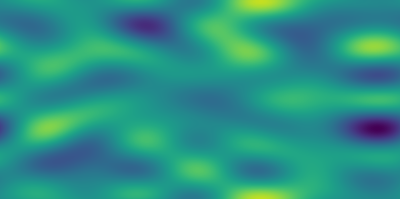
\includegraphics[interpolate=false,width=1.000000in,height=1.000000in]{burgers_rollout_target_0.01-img0.png}}%
\end{pgfscope}%
\begin{pgfscope}%
\pgfsetbuttcap%
\pgfsetroundjoin%
\definecolor{currentfill}{rgb}{0.000000,0.000000,0.000000}%
\pgfsetfillcolor{currentfill}%
\pgfsetlinewidth{0.803000pt}%
\definecolor{currentstroke}{rgb}{0.000000,0.000000,0.000000}%
\pgfsetstrokecolor{currentstroke}%
\pgfsetdash{}{0pt}%
\pgfsys@defobject{currentmarker}{\pgfqpoint{0.000000in}{-0.048611in}}{\pgfqpoint{0.000000in}{0.000000in}}{%
\pgfpathmoveto{\pgfqpoint{0.000000in}{0.000000in}}%
\pgfpathlineto{\pgfqpoint{0.000000in}{-0.048611in}}%
\pgfusepath{stroke,fill}%
}%
\begin{pgfscope}%
\pgfsys@transformshift{0.726837in}{0.517039in}%
\pgfsys@useobject{currentmarker}{}%
\end{pgfscope}%
\end{pgfscope}%
\begin{pgfscope}%
\definecolor{textcolor}{rgb}{0.000000,0.000000,0.000000}%
\pgfsetstrokecolor{textcolor}%
\pgfsetfillcolor{textcolor}%
\pgftext[x=0.726837in,y=0.419816in,,top]{\color{textcolor}\rmfamily\fontsize{12.000000}{14.400000}\selectfont 0}%
\end{pgfscope}%
\begin{pgfscope}%
\pgfsetbuttcap%
\pgfsetroundjoin%
\definecolor{currentfill}{rgb}{0.000000,0.000000,0.000000}%
\pgfsetfillcolor{currentfill}%
\pgfsetlinewidth{0.803000pt}%
\definecolor{currentstroke}{rgb}{0.000000,0.000000,0.000000}%
\pgfsetstrokecolor{currentstroke}%
\pgfsetdash{}{0pt}%
\pgfsys@defobject{currentmarker}{\pgfqpoint{0.000000in}{-0.048611in}}{\pgfqpoint{0.000000in}{0.000000in}}{%
\pgfpathmoveto{\pgfqpoint{0.000000in}{0.000000in}}%
\pgfpathlineto{\pgfqpoint{0.000000in}{-0.048611in}}%
\pgfusepath{stroke,fill}%
}%
\begin{pgfscope}%
\pgfsys@transformshift{1.570762in}{0.517039in}%
\pgfsys@useobject{currentmarker}{}%
\end{pgfscope}%
\end{pgfscope}%
\begin{pgfscope}%
\definecolor{textcolor}{rgb}{0.000000,0.000000,0.000000}%
\pgfsetstrokecolor{textcolor}%
\pgfsetfillcolor{textcolor}%
\pgftext[x=1.570762in,y=0.419816in,,top]{\color{textcolor}\rmfamily\fontsize{12.000000}{14.400000}\selectfont 1}%
\end{pgfscope}%
\begin{pgfscope}%
\pgfsetbuttcap%
\pgfsetroundjoin%
\definecolor{currentfill}{rgb}{0.000000,0.000000,0.000000}%
\pgfsetfillcolor{currentfill}%
\pgfsetlinewidth{0.803000pt}%
\definecolor{currentstroke}{rgb}{0.000000,0.000000,0.000000}%
\pgfsetstrokecolor{currentstroke}%
\pgfsetdash{}{0pt}%
\pgfsys@defobject{currentmarker}{\pgfqpoint{0.000000in}{-0.048611in}}{\pgfqpoint{0.000000in}{0.000000in}}{%
\pgfpathmoveto{\pgfqpoint{0.000000in}{0.000000in}}%
\pgfpathlineto{\pgfqpoint{0.000000in}{-0.048611in}}%
\pgfusepath{stroke,fill}%
}%
\begin{pgfscope}%
\pgfsys@transformshift{2.414687in}{0.517039in}%
\pgfsys@useobject{currentmarker}{}%
\end{pgfscope}%
\end{pgfscope}%
\begin{pgfscope}%
\definecolor{textcolor}{rgb}{0.000000,0.000000,0.000000}%
\pgfsetstrokecolor{textcolor}%
\pgfsetfillcolor{textcolor}%
\pgftext[x=2.414687in,y=0.419816in,,top]{\color{textcolor}\rmfamily\fontsize{12.000000}{14.400000}\selectfont 2}%
\end{pgfscope}%
\begin{pgfscope}%
\definecolor{textcolor}{rgb}{0.000000,0.000000,0.000000}%
\pgfsetstrokecolor{textcolor}%
\pgfsetfillcolor{textcolor}%
\pgftext[x=1.570762in,y=0.202965in,,top]{\color{textcolor}\rmfamily\fontsize{12.000000}{14.400000}\selectfont Space}%
\end{pgfscope}%
\begin{pgfscope}%
\pgfsetbuttcap%
\pgfsetroundjoin%
\definecolor{currentfill}{rgb}{0.000000,0.000000,0.000000}%
\pgfsetfillcolor{currentfill}%
\pgfsetlinewidth{0.803000pt}%
\definecolor{currentstroke}{rgb}{0.000000,0.000000,0.000000}%
\pgfsetstrokecolor{currentstroke}%
\pgfsetdash{}{0pt}%
\pgfsys@defobject{currentmarker}{\pgfqpoint{-0.048611in}{0.000000in}}{\pgfqpoint{-0.000000in}{0.000000in}}{%
\pgfpathmoveto{\pgfqpoint{-0.000000in}{0.000000in}}%
\pgfpathlineto{\pgfqpoint{-0.048611in}{0.000000in}}%
\pgfusepath{stroke,fill}%
}%
\begin{pgfscope}%
\pgfsys@transformshift{0.726837in}{0.517039in}%
\pgfsys@useobject{currentmarker}{}%
\end{pgfscope}%
\end{pgfscope}%
\begin{pgfscope}%
\definecolor{textcolor}{rgb}{0.000000,0.000000,0.000000}%
\pgfsetstrokecolor{textcolor}%
\pgfsetfillcolor{textcolor}%
\pgftext[x=0.364559in, y=0.453725in, left, base]{\color{textcolor}\rmfamily\fontsize{12.000000}{14.400000}\selectfont 0.0}%
\end{pgfscope}%
\begin{pgfscope}%
\pgfsetbuttcap%
\pgfsetroundjoin%
\definecolor{currentfill}{rgb}{0.000000,0.000000,0.000000}%
\pgfsetfillcolor{currentfill}%
\pgfsetlinewidth{0.803000pt}%
\definecolor{currentstroke}{rgb}{0.000000,0.000000,0.000000}%
\pgfsetstrokecolor{currentstroke}%
\pgfsetdash{}{0pt}%
\pgfsys@defobject{currentmarker}{\pgfqpoint{-0.048611in}{0.000000in}}{\pgfqpoint{-0.000000in}{0.000000in}}{%
\pgfpathmoveto{\pgfqpoint{-0.000000in}{0.000000in}}%
\pgfpathlineto{\pgfqpoint{-0.048611in}{0.000000in}}%
\pgfusepath{stroke,fill}%
}%
\begin{pgfscope}%
\pgfsys@transformshift{0.726837in}{0.861533in}%
\pgfsys@useobject{currentmarker}{}%
\end{pgfscope}%
\end{pgfscope}%
\begin{pgfscope}%
\definecolor{textcolor}{rgb}{0.000000,0.000000,0.000000}%
\pgfsetstrokecolor{textcolor}%
\pgfsetfillcolor{textcolor}%
\pgftext[x=0.364559in, y=0.798219in, left, base]{\color{textcolor}\rmfamily\fontsize{12.000000}{14.400000}\selectfont 2.5}%
\end{pgfscope}%
\begin{pgfscope}%
\pgfsetbuttcap%
\pgfsetroundjoin%
\definecolor{currentfill}{rgb}{0.000000,0.000000,0.000000}%
\pgfsetfillcolor{currentfill}%
\pgfsetlinewidth{0.803000pt}%
\definecolor{currentstroke}{rgb}{0.000000,0.000000,0.000000}%
\pgfsetstrokecolor{currentstroke}%
\pgfsetdash{}{0pt}%
\pgfsys@defobject{currentmarker}{\pgfqpoint{-0.048611in}{0.000000in}}{\pgfqpoint{-0.000000in}{0.000000in}}{%
\pgfpathmoveto{\pgfqpoint{-0.000000in}{0.000000in}}%
\pgfpathlineto{\pgfqpoint{-0.048611in}{0.000000in}}%
\pgfusepath{stroke,fill}%
}%
\begin{pgfscope}%
\pgfsys@transformshift{0.726837in}{1.206027in}%
\pgfsys@useobject{currentmarker}{}%
\end{pgfscope}%
\end{pgfscope}%
\begin{pgfscope}%
\definecolor{textcolor}{rgb}{0.000000,0.000000,0.000000}%
\pgfsetstrokecolor{textcolor}%
\pgfsetfillcolor{textcolor}%
\pgftext[x=0.364559in, y=1.142714in, left, base]{\color{textcolor}\rmfamily\fontsize{12.000000}{14.400000}\selectfont 5.0}%
\end{pgfscope}%
\begin{pgfscope}%
\pgfsetbuttcap%
\pgfsetroundjoin%
\definecolor{currentfill}{rgb}{0.000000,0.000000,0.000000}%
\pgfsetfillcolor{currentfill}%
\pgfsetlinewidth{0.803000pt}%
\definecolor{currentstroke}{rgb}{0.000000,0.000000,0.000000}%
\pgfsetstrokecolor{currentstroke}%
\pgfsetdash{}{0pt}%
\pgfsys@defobject{currentmarker}{\pgfqpoint{-0.048611in}{0.000000in}}{\pgfqpoint{-0.000000in}{0.000000in}}{%
\pgfpathmoveto{\pgfqpoint{-0.000000in}{0.000000in}}%
\pgfpathlineto{\pgfqpoint{-0.048611in}{0.000000in}}%
\pgfusepath{stroke,fill}%
}%
\begin{pgfscope}%
\pgfsys@transformshift{0.726837in}{1.550522in}%
\pgfsys@useobject{currentmarker}{}%
\end{pgfscope}%
\end{pgfscope}%
\begin{pgfscope}%
\definecolor{textcolor}{rgb}{0.000000,0.000000,0.000000}%
\pgfsetstrokecolor{textcolor}%
\pgfsetfillcolor{textcolor}%
\pgftext[x=0.364559in, y=1.487208in, left, base]{\color{textcolor}\rmfamily\fontsize{12.000000}{14.400000}\selectfont 7.5}%
\end{pgfscope}%
\begin{pgfscope}%
\pgfsetbuttcap%
\pgfsetroundjoin%
\definecolor{currentfill}{rgb}{0.000000,0.000000,0.000000}%
\pgfsetfillcolor{currentfill}%
\pgfsetlinewidth{0.803000pt}%
\definecolor{currentstroke}{rgb}{0.000000,0.000000,0.000000}%
\pgfsetstrokecolor{currentstroke}%
\pgfsetdash{}{0pt}%
\pgfsys@defobject{currentmarker}{\pgfqpoint{-0.048611in}{0.000000in}}{\pgfqpoint{-0.000000in}{0.000000in}}{%
\pgfpathmoveto{\pgfqpoint{-0.000000in}{0.000000in}}%
\pgfpathlineto{\pgfqpoint{-0.048611in}{0.000000in}}%
\pgfusepath{stroke,fill}%
}%
\begin{pgfscope}%
\pgfsys@transformshift{0.726837in}{1.895016in}%
\pgfsys@useobject{currentmarker}{}%
\end{pgfscope}%
\end{pgfscope}%
\begin{pgfscope}%
\definecolor{textcolor}{rgb}{0.000000,0.000000,0.000000}%
\pgfsetstrokecolor{textcolor}%
\pgfsetfillcolor{textcolor}%
\pgftext[x=0.258521in, y=1.831702in, left, base]{\color{textcolor}\rmfamily\fontsize{12.000000}{14.400000}\selectfont 10.0}%
\end{pgfscope}%
\begin{pgfscope}%
\definecolor{textcolor}{rgb}{0.000000,0.000000,0.000000}%
\pgfsetstrokecolor{textcolor}%
\pgfsetfillcolor{textcolor}%
\pgftext[x=0.202965in,y=1.206027in,,bottom,rotate=90.000000]{\color{textcolor}\rmfamily\fontsize{12.000000}{14.400000}\selectfont Time}%
\end{pgfscope}%
\begin{pgfscope}%
\pgfsetrectcap%
\pgfsetmiterjoin%
\pgfsetlinewidth{0.803000pt}%
\definecolor{currentstroke}{rgb}{0.000000,0.000000,0.000000}%
\pgfsetstrokecolor{currentstroke}%
\pgfsetdash{}{0pt}%
\pgfpathmoveto{\pgfqpoint{0.726837in}{0.517039in}}%
\pgfpathlineto{\pgfqpoint{0.726837in}{1.895016in}}%
\pgfusepath{stroke}%
\end{pgfscope}%
\begin{pgfscope}%
\pgfsetrectcap%
\pgfsetmiterjoin%
\pgfsetlinewidth{0.803000pt}%
\definecolor{currentstroke}{rgb}{0.000000,0.000000,0.000000}%
\pgfsetstrokecolor{currentstroke}%
\pgfsetdash{}{0pt}%
\pgfpathmoveto{\pgfqpoint{2.414687in}{0.517039in}}%
\pgfpathlineto{\pgfqpoint{2.414687in}{1.895016in}}%
\pgfusepath{stroke}%
\end{pgfscope}%
\begin{pgfscope}%
\pgfsetrectcap%
\pgfsetmiterjoin%
\pgfsetlinewidth{0.803000pt}%
\definecolor{currentstroke}{rgb}{0.000000,0.000000,0.000000}%
\pgfsetstrokecolor{currentstroke}%
\pgfsetdash{}{0pt}%
\pgfpathmoveto{\pgfqpoint{0.726837in}{0.517039in}}%
\pgfpathlineto{\pgfqpoint{2.414687in}{0.517039in}}%
\pgfusepath{stroke}%
\end{pgfscope}%
\begin{pgfscope}%
\pgfsetrectcap%
\pgfsetmiterjoin%
\pgfsetlinewidth{0.803000pt}%
\definecolor{currentstroke}{rgb}{0.000000,0.000000,0.000000}%
\pgfsetstrokecolor{currentstroke}%
\pgfsetdash{}{0pt}%
\pgfpathmoveto{\pgfqpoint{0.726837in}{1.895016in}}%
\pgfpathlineto{\pgfqpoint{2.414687in}{1.895016in}}%
\pgfusepath{stroke}%
\end{pgfscope}%
\begin{pgfscope}%
\pgfsetbuttcap%
\pgfsetmiterjoin%
\pgfsetlinewidth{0.000000pt}%
\definecolor{currentstroke}{rgb}{0.000000,0.000000,0.000000}%
\pgfsetstrokecolor{currentstroke}%
\pgfsetstrokeopacity{0.000000}%
\pgfsetdash{}{0pt}%
\pgfpathmoveto{\pgfqpoint{2.552099in}{0.517039in}}%
\pgfpathlineto{\pgfqpoint{2.620998in}{0.517039in}}%
\pgfpathlineto{\pgfqpoint{2.620998in}{1.895016in}}%
\pgfpathlineto{\pgfqpoint{2.552099in}{1.895016in}}%
\pgfpathlineto{\pgfqpoint{2.552099in}{0.517039in}}%
\pgfpathclose%
\pgfusepath{}%
\end{pgfscope}%
\begin{pgfscope}%
\pgfsys@transformshift{2.550000in}{0.520000in}%
\pgftext[left,bottom]{
\includegraphics[interpolate=true,width=0.070000in,height=1.380000in]{burgers_rollout_target_0.01-img1.png}}%
\end{pgfscope}%
\begin{pgfscope}%
\pgfsetbuttcap%
\pgfsetroundjoin%
\definecolor{currentfill}{rgb}{0.000000,0.000000,0.000000}%
\pgfsetfillcolor{currentfill}%
\pgfsetlinewidth{0.803000pt}%
\definecolor{currentstroke}{rgb}{0.000000,0.000000,0.000000}%
\pgfsetstrokecolor{currentstroke}%
\pgfsetdash{}{0pt}%
\pgfsys@defobject{currentmarker}{\pgfqpoint{0.000000in}{0.000000in}}{\pgfqpoint{0.048611in}{0.000000in}}{%
\pgfpathmoveto{\pgfqpoint{0.000000in}{0.000000in}}%
\pgfpathlineto{\pgfqpoint{0.048611in}{0.000000in}}%
\pgfusepath{stroke,fill}%
}%
\begin{pgfscope}%
\pgfsys@transformshift{2.620998in}{0.588723in}%
\pgfsys@useobject{currentmarker}{}%
\end{pgfscope}%
\end{pgfscope}%
\begin{pgfscope}%
\definecolor{textcolor}{rgb}{0.000000,0.000000,0.000000}%
\pgfsetstrokecolor{textcolor}%
\pgfsetfillcolor{textcolor}%
\pgftext[x=2.718220in, y=0.525410in, left, base]{\color{textcolor}\rmfamily\fontsize{12.000000}{14.400000}\selectfont \ensuremath{-}1}%
\end{pgfscope}%
\begin{pgfscope}%
\pgfsetbuttcap%
\pgfsetroundjoin%
\definecolor{currentfill}{rgb}{0.000000,0.000000,0.000000}%
\pgfsetfillcolor{currentfill}%
\pgfsetlinewidth{0.803000pt}%
\definecolor{currentstroke}{rgb}{0.000000,0.000000,0.000000}%
\pgfsetstrokecolor{currentstroke}%
\pgfsetdash{}{0pt}%
\pgfsys@defobject{currentmarker}{\pgfqpoint{0.000000in}{0.000000in}}{\pgfqpoint{0.048611in}{0.000000in}}{%
\pgfpathmoveto{\pgfqpoint{0.000000in}{0.000000in}}%
\pgfpathlineto{\pgfqpoint{0.048611in}{0.000000in}}%
\pgfusepath{stroke,fill}%
}%
\begin{pgfscope}%
\pgfsys@transformshift{2.620998in}{1.206027in}%
\pgfsys@useobject{currentmarker}{}%
\end{pgfscope}%
\end{pgfscope}%
\begin{pgfscope}%
\definecolor{textcolor}{rgb}{0.000000,0.000000,0.000000}%
\pgfsetstrokecolor{textcolor}%
\pgfsetfillcolor{textcolor}%
\pgftext[x=2.718220in, y=1.142714in, left, base]{\color{textcolor}\rmfamily\fontsize{12.000000}{14.400000}\selectfont 0}%
\end{pgfscope}%
\begin{pgfscope}%
\pgfsetbuttcap%
\pgfsetroundjoin%
\definecolor{currentfill}{rgb}{0.000000,0.000000,0.000000}%
\pgfsetfillcolor{currentfill}%
\pgfsetlinewidth{0.803000pt}%
\definecolor{currentstroke}{rgb}{0.000000,0.000000,0.000000}%
\pgfsetstrokecolor{currentstroke}%
\pgfsetdash{}{0pt}%
\pgfsys@defobject{currentmarker}{\pgfqpoint{0.000000in}{0.000000in}}{\pgfqpoint{0.048611in}{0.000000in}}{%
\pgfpathmoveto{\pgfqpoint{0.000000in}{0.000000in}}%
\pgfpathlineto{\pgfqpoint{0.048611in}{0.000000in}}%
\pgfusepath{stroke,fill}%
}%
\begin{pgfscope}%
\pgfsys@transformshift{2.620998in}{1.823331in}%
\pgfsys@useobject{currentmarker}{}%
\end{pgfscope}%
\end{pgfscope}%
\begin{pgfscope}%
\definecolor{textcolor}{rgb}{0.000000,0.000000,0.000000}%
\pgfsetstrokecolor{textcolor}%
\pgfsetfillcolor{textcolor}%
\pgftext[x=2.718220in, y=1.760018in, left, base]{\color{textcolor}\rmfamily\fontsize{12.000000}{14.400000}\selectfont 1}%
\end{pgfscope}%
\begin{pgfscope}%
\pgfsetrectcap%
\pgfsetmiterjoin%
\pgfsetlinewidth{0.803000pt}%
\definecolor{currentstroke}{rgb}{0.000000,0.000000,0.000000}%
\pgfsetstrokecolor{currentstroke}%
\pgfsetdash{}{0pt}%
\pgfpathmoveto{\pgfqpoint{2.552099in}{0.517039in}}%
\pgfpathlineto{\pgfqpoint{2.586548in}{0.517039in}}%
\pgfpathlineto{\pgfqpoint{2.620998in}{0.517039in}}%
\pgfpathlineto{\pgfqpoint{2.620998in}{1.895016in}}%
\pgfpathlineto{\pgfqpoint{2.586548in}{1.895016in}}%
\pgfpathlineto{\pgfqpoint{2.552099in}{1.895016in}}%
\pgfpathlineto{\pgfqpoint{2.552099in}{0.517039in}}%
\pgfpathclose%
\pgfusepath{stroke}%
\end{pgfscope}%
\end{pgfpicture}%
\makeatother%
\endgroup%

      \end{adjustbox}
      \caption{The target for \(\nu=0.01\)}\label{fig:sc2_rollout_target_0.01}
    \end{subfigure}
    \begin{subfigure}{0.33\linewidth}
      \begin{adjustbox}{width=\linewidth}
        \begingroup%
\makeatletter%
\begin{pgfpicture}%
\pgfpathrectangle{\pgfpointorigin}{\pgfqpoint{3.000000in}{2.000000in}}%
\pgfusepath{use as bounding box, clip}%
\begin{pgfscope}%
\pgfsetbuttcap%
\pgfsetmiterjoin%
\pgfsetlinewidth{0.000000pt}%
\definecolor{currentstroke}{rgb}{0.000000,0.000000,0.000000}%
\pgfsetstrokecolor{currentstroke}%
\pgfsetstrokeopacity{0.000000}%
\pgfsetdash{}{0pt}%
\pgfpathmoveto{\pgfqpoint{0.000000in}{0.000000in}}%
\pgfpathlineto{\pgfqpoint{3.000000in}{0.000000in}}%
\pgfpathlineto{\pgfqpoint{3.000000in}{2.000000in}}%
\pgfpathlineto{\pgfqpoint{0.000000in}{2.000000in}}%
\pgfpathlineto{\pgfqpoint{0.000000in}{0.000000in}}%
\pgfpathclose%
\pgfusepath{}%
\end{pgfscope}%
\begin{pgfscope}%
\pgfsetbuttcap%
\pgfsetmiterjoin%
\pgfsetlinewidth{0.000000pt}%
\definecolor{currentstroke}{rgb}{0.000000,0.000000,0.000000}%
\pgfsetstrokecolor{currentstroke}%
\pgfsetstrokeopacity{0.000000}%
\pgfsetdash{}{0pt}%
\pgfpathmoveto{\pgfqpoint{0.726837in}{0.517039in}}%
\pgfpathlineto{\pgfqpoint{2.414687in}{0.517039in}}%
\pgfpathlineto{\pgfqpoint{2.414687in}{1.895016in}}%
\pgfpathlineto{\pgfqpoint{0.726837in}{1.895016in}}%
\pgfpathlineto{\pgfqpoint{0.726837in}{0.517039in}}%
\pgfpathclose%
\pgfusepath{}%
\end{pgfscope}%
\begin{pgfscope}%
\pgfpathrectangle{\pgfqpoint{0.726837in}{0.517039in}}{\pgfqpoint{1.687850in}{1.377978in}}%
\pgfusepath{clip}%
\pgfsys@transformcm{1.687850}{0.000000}{0.000000}{1.377978}{0.726837in}{0.517039in}%
\pgftext[left,bottom]{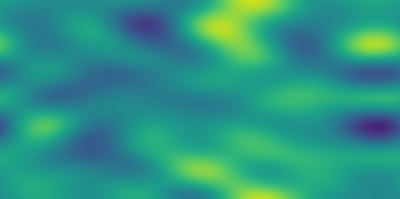
\includegraphics[interpolate=false,width=1.000000in,height=1.000000in]{burgers_rollout_pred_0.01-img0.png}}%
\end{pgfscope}%
\begin{pgfscope}%
\pgfsetbuttcap%
\pgfsetroundjoin%
\definecolor{currentfill}{rgb}{0.000000,0.000000,0.000000}%
\pgfsetfillcolor{currentfill}%
\pgfsetlinewidth{0.803000pt}%
\definecolor{currentstroke}{rgb}{0.000000,0.000000,0.000000}%
\pgfsetstrokecolor{currentstroke}%
\pgfsetdash{}{0pt}%
\pgfsys@defobject{currentmarker}{\pgfqpoint{0.000000in}{-0.048611in}}{\pgfqpoint{0.000000in}{0.000000in}}{%
\pgfpathmoveto{\pgfqpoint{0.000000in}{0.000000in}}%
\pgfpathlineto{\pgfqpoint{0.000000in}{-0.048611in}}%
\pgfusepath{stroke,fill}%
}%
\begin{pgfscope}%
\pgfsys@transformshift{0.726837in}{0.517039in}%
\pgfsys@useobject{currentmarker}{}%
\end{pgfscope}%
\end{pgfscope}%
\begin{pgfscope}%
\definecolor{textcolor}{rgb}{0.000000,0.000000,0.000000}%
\pgfsetstrokecolor{textcolor}%
\pgfsetfillcolor{textcolor}%
\pgftext[x=0.726837in,y=0.419816in,,top]{\color{textcolor}{\rmfamily\fontsize{12.000000}{14.400000}\selectfont\catcode`\^=\active\def^{\ifmmode\sp\else\^{}\fi}\catcode`\%=\active\def%{\%}0}}%
\end{pgfscope}%
\begin{pgfscope}%
\pgfsetbuttcap%
\pgfsetroundjoin%
\definecolor{currentfill}{rgb}{0.000000,0.000000,0.000000}%
\pgfsetfillcolor{currentfill}%
\pgfsetlinewidth{0.803000pt}%
\definecolor{currentstroke}{rgb}{0.000000,0.000000,0.000000}%
\pgfsetstrokecolor{currentstroke}%
\pgfsetdash{}{0pt}%
\pgfsys@defobject{currentmarker}{\pgfqpoint{0.000000in}{-0.048611in}}{\pgfqpoint{0.000000in}{0.000000in}}{%
\pgfpathmoveto{\pgfqpoint{0.000000in}{0.000000in}}%
\pgfpathlineto{\pgfqpoint{0.000000in}{-0.048611in}}%
\pgfusepath{stroke,fill}%
}%
\begin{pgfscope}%
\pgfsys@transformshift{1.570762in}{0.517039in}%
\pgfsys@useobject{currentmarker}{}%
\end{pgfscope}%
\end{pgfscope}%
\begin{pgfscope}%
\definecolor{textcolor}{rgb}{0.000000,0.000000,0.000000}%
\pgfsetstrokecolor{textcolor}%
\pgfsetfillcolor{textcolor}%
\pgftext[x=1.570762in,y=0.419816in,,top]{\color{textcolor}{\rmfamily\fontsize{12.000000}{14.400000}\selectfont\catcode`\^=\active\def^{\ifmmode\sp\else\^{}\fi}\catcode`\%=\active\def%{\%}1}}%
\end{pgfscope}%
\begin{pgfscope}%
\pgfsetbuttcap%
\pgfsetroundjoin%
\definecolor{currentfill}{rgb}{0.000000,0.000000,0.000000}%
\pgfsetfillcolor{currentfill}%
\pgfsetlinewidth{0.803000pt}%
\definecolor{currentstroke}{rgb}{0.000000,0.000000,0.000000}%
\pgfsetstrokecolor{currentstroke}%
\pgfsetdash{}{0pt}%
\pgfsys@defobject{currentmarker}{\pgfqpoint{0.000000in}{-0.048611in}}{\pgfqpoint{0.000000in}{0.000000in}}{%
\pgfpathmoveto{\pgfqpoint{0.000000in}{0.000000in}}%
\pgfpathlineto{\pgfqpoint{0.000000in}{-0.048611in}}%
\pgfusepath{stroke,fill}%
}%
\begin{pgfscope}%
\pgfsys@transformshift{2.414687in}{0.517039in}%
\pgfsys@useobject{currentmarker}{}%
\end{pgfscope}%
\end{pgfscope}%
\begin{pgfscope}%
\definecolor{textcolor}{rgb}{0.000000,0.000000,0.000000}%
\pgfsetstrokecolor{textcolor}%
\pgfsetfillcolor{textcolor}%
\pgftext[x=2.414687in,y=0.419816in,,top]{\color{textcolor}{\rmfamily\fontsize{12.000000}{14.400000}\selectfont\catcode`\^=\active\def^{\ifmmode\sp\else\^{}\fi}\catcode`\%=\active\def%{\%}2}}%
\end{pgfscope}%
\begin{pgfscope}%
\definecolor{textcolor}{rgb}{0.000000,0.000000,0.000000}%
\pgfsetstrokecolor{textcolor}%
\pgfsetfillcolor{textcolor}%
\pgftext[x=1.570762in,y=0.202965in,,top]{\color{textcolor}{\rmfamily\fontsize{12.000000}{14.400000}\selectfont\catcode`\^=\active\def^{\ifmmode\sp\else\^{}\fi}\catcode`\%=\active\def%{\%}Space}}%
\end{pgfscope}%
\begin{pgfscope}%
\pgfsetbuttcap%
\pgfsetroundjoin%
\definecolor{currentfill}{rgb}{0.000000,0.000000,0.000000}%
\pgfsetfillcolor{currentfill}%
\pgfsetlinewidth{0.803000pt}%
\definecolor{currentstroke}{rgb}{0.000000,0.000000,0.000000}%
\pgfsetstrokecolor{currentstroke}%
\pgfsetdash{}{0pt}%
\pgfsys@defobject{currentmarker}{\pgfqpoint{-0.048611in}{0.000000in}}{\pgfqpoint{-0.000000in}{0.000000in}}{%
\pgfpathmoveto{\pgfqpoint{-0.000000in}{0.000000in}}%
\pgfpathlineto{\pgfqpoint{-0.048611in}{0.000000in}}%
\pgfusepath{stroke,fill}%
}%
\begin{pgfscope}%
\pgfsys@transformshift{0.726837in}{0.517039in}%
\pgfsys@useobject{currentmarker}{}%
\end{pgfscope}%
\end{pgfscope}%
\begin{pgfscope}%
\definecolor{textcolor}{rgb}{0.000000,0.000000,0.000000}%
\pgfsetstrokecolor{textcolor}%
\pgfsetfillcolor{textcolor}%
\pgftext[x=0.364559in, y=0.453725in, left, base]{\color{textcolor}{\rmfamily\fontsize{12.000000}{14.400000}\selectfont\catcode`\^=\active\def^{\ifmmode\sp\else\^{}\fi}\catcode`\%=\active\def%{\%}0.0}}%
\end{pgfscope}%
\begin{pgfscope}%
\pgfsetbuttcap%
\pgfsetroundjoin%
\definecolor{currentfill}{rgb}{0.000000,0.000000,0.000000}%
\pgfsetfillcolor{currentfill}%
\pgfsetlinewidth{0.803000pt}%
\definecolor{currentstroke}{rgb}{0.000000,0.000000,0.000000}%
\pgfsetstrokecolor{currentstroke}%
\pgfsetdash{}{0pt}%
\pgfsys@defobject{currentmarker}{\pgfqpoint{-0.048611in}{0.000000in}}{\pgfqpoint{-0.000000in}{0.000000in}}{%
\pgfpathmoveto{\pgfqpoint{-0.000000in}{0.000000in}}%
\pgfpathlineto{\pgfqpoint{-0.048611in}{0.000000in}}%
\pgfusepath{stroke,fill}%
}%
\begin{pgfscope}%
\pgfsys@transformshift{0.726837in}{0.861533in}%
\pgfsys@useobject{currentmarker}{}%
\end{pgfscope}%
\end{pgfscope}%
\begin{pgfscope}%
\definecolor{textcolor}{rgb}{0.000000,0.000000,0.000000}%
\pgfsetstrokecolor{textcolor}%
\pgfsetfillcolor{textcolor}%
\pgftext[x=0.364559in, y=0.798219in, left, base]{\color{textcolor}{\rmfamily\fontsize{12.000000}{14.400000}\selectfont\catcode`\^=\active\def^{\ifmmode\sp\else\^{}\fi}\catcode`\%=\active\def%{\%}2.5}}%
\end{pgfscope}%
\begin{pgfscope}%
\pgfsetbuttcap%
\pgfsetroundjoin%
\definecolor{currentfill}{rgb}{0.000000,0.000000,0.000000}%
\pgfsetfillcolor{currentfill}%
\pgfsetlinewidth{0.803000pt}%
\definecolor{currentstroke}{rgb}{0.000000,0.000000,0.000000}%
\pgfsetstrokecolor{currentstroke}%
\pgfsetdash{}{0pt}%
\pgfsys@defobject{currentmarker}{\pgfqpoint{-0.048611in}{0.000000in}}{\pgfqpoint{-0.000000in}{0.000000in}}{%
\pgfpathmoveto{\pgfqpoint{-0.000000in}{0.000000in}}%
\pgfpathlineto{\pgfqpoint{-0.048611in}{0.000000in}}%
\pgfusepath{stroke,fill}%
}%
\begin{pgfscope}%
\pgfsys@transformshift{0.726837in}{1.206027in}%
\pgfsys@useobject{currentmarker}{}%
\end{pgfscope}%
\end{pgfscope}%
\begin{pgfscope}%
\definecolor{textcolor}{rgb}{0.000000,0.000000,0.000000}%
\pgfsetstrokecolor{textcolor}%
\pgfsetfillcolor{textcolor}%
\pgftext[x=0.364559in, y=1.142714in, left, base]{\color{textcolor}{\rmfamily\fontsize{12.000000}{14.400000}\selectfont\catcode`\^=\active\def^{\ifmmode\sp\else\^{}\fi}\catcode`\%=\active\def%{\%}5.0}}%
\end{pgfscope}%
\begin{pgfscope}%
\pgfsetbuttcap%
\pgfsetroundjoin%
\definecolor{currentfill}{rgb}{0.000000,0.000000,0.000000}%
\pgfsetfillcolor{currentfill}%
\pgfsetlinewidth{0.803000pt}%
\definecolor{currentstroke}{rgb}{0.000000,0.000000,0.000000}%
\pgfsetstrokecolor{currentstroke}%
\pgfsetdash{}{0pt}%
\pgfsys@defobject{currentmarker}{\pgfqpoint{-0.048611in}{0.000000in}}{\pgfqpoint{-0.000000in}{0.000000in}}{%
\pgfpathmoveto{\pgfqpoint{-0.000000in}{0.000000in}}%
\pgfpathlineto{\pgfqpoint{-0.048611in}{0.000000in}}%
\pgfusepath{stroke,fill}%
}%
\begin{pgfscope}%
\pgfsys@transformshift{0.726837in}{1.550522in}%
\pgfsys@useobject{currentmarker}{}%
\end{pgfscope}%
\end{pgfscope}%
\begin{pgfscope}%
\definecolor{textcolor}{rgb}{0.000000,0.000000,0.000000}%
\pgfsetstrokecolor{textcolor}%
\pgfsetfillcolor{textcolor}%
\pgftext[x=0.364559in, y=1.487208in, left, base]{\color{textcolor}{\rmfamily\fontsize{12.000000}{14.400000}\selectfont\catcode`\^=\active\def^{\ifmmode\sp\else\^{}\fi}\catcode`\%=\active\def%{\%}7.5}}%
\end{pgfscope}%
\begin{pgfscope}%
\pgfsetbuttcap%
\pgfsetroundjoin%
\definecolor{currentfill}{rgb}{0.000000,0.000000,0.000000}%
\pgfsetfillcolor{currentfill}%
\pgfsetlinewidth{0.803000pt}%
\definecolor{currentstroke}{rgb}{0.000000,0.000000,0.000000}%
\pgfsetstrokecolor{currentstroke}%
\pgfsetdash{}{0pt}%
\pgfsys@defobject{currentmarker}{\pgfqpoint{-0.048611in}{0.000000in}}{\pgfqpoint{-0.000000in}{0.000000in}}{%
\pgfpathmoveto{\pgfqpoint{-0.000000in}{0.000000in}}%
\pgfpathlineto{\pgfqpoint{-0.048611in}{0.000000in}}%
\pgfusepath{stroke,fill}%
}%
\begin{pgfscope}%
\pgfsys@transformshift{0.726837in}{1.895016in}%
\pgfsys@useobject{currentmarker}{}%
\end{pgfscope}%
\end{pgfscope}%
\begin{pgfscope}%
\definecolor{textcolor}{rgb}{0.000000,0.000000,0.000000}%
\pgfsetstrokecolor{textcolor}%
\pgfsetfillcolor{textcolor}%
\pgftext[x=0.258521in, y=1.831702in, left, base]{\color{textcolor}{\rmfamily\fontsize{12.000000}{14.400000}\selectfont\catcode`\^=\active\def^{\ifmmode\sp\else\^{}\fi}\catcode`\%=\active\def%{\%}10.0}}%
\end{pgfscope}%
\begin{pgfscope}%
\definecolor{textcolor}{rgb}{0.000000,0.000000,0.000000}%
\pgfsetstrokecolor{textcolor}%
\pgfsetfillcolor{textcolor}%
\pgftext[x=0.202965in,y=1.206027in,,bottom,rotate=90.000000]{\color{textcolor}{\rmfamily\fontsize{12.000000}{14.400000}\selectfont\catcode`\^=\active\def^{\ifmmode\sp\else\^{}\fi}\catcode`\%=\active\def%{\%}Time}}%
\end{pgfscope}%
\begin{pgfscope}%
\pgfsetrectcap%
\pgfsetmiterjoin%
\pgfsetlinewidth{0.803000pt}%
\definecolor{currentstroke}{rgb}{0.000000,0.000000,0.000000}%
\pgfsetstrokecolor{currentstroke}%
\pgfsetdash{}{0pt}%
\pgfpathmoveto{\pgfqpoint{0.726837in}{0.517039in}}%
\pgfpathlineto{\pgfqpoint{0.726837in}{1.895016in}}%
\pgfusepath{stroke}%
\end{pgfscope}%
\begin{pgfscope}%
\pgfsetrectcap%
\pgfsetmiterjoin%
\pgfsetlinewidth{0.803000pt}%
\definecolor{currentstroke}{rgb}{0.000000,0.000000,0.000000}%
\pgfsetstrokecolor{currentstroke}%
\pgfsetdash{}{0pt}%
\pgfpathmoveto{\pgfqpoint{2.414687in}{0.517039in}}%
\pgfpathlineto{\pgfqpoint{2.414687in}{1.895016in}}%
\pgfusepath{stroke}%
\end{pgfscope}%
\begin{pgfscope}%
\pgfsetrectcap%
\pgfsetmiterjoin%
\pgfsetlinewidth{0.803000pt}%
\definecolor{currentstroke}{rgb}{0.000000,0.000000,0.000000}%
\pgfsetstrokecolor{currentstroke}%
\pgfsetdash{}{0pt}%
\pgfpathmoveto{\pgfqpoint{0.726837in}{0.517039in}}%
\pgfpathlineto{\pgfqpoint{2.414687in}{0.517039in}}%
\pgfusepath{stroke}%
\end{pgfscope}%
\begin{pgfscope}%
\pgfsetrectcap%
\pgfsetmiterjoin%
\pgfsetlinewidth{0.803000pt}%
\definecolor{currentstroke}{rgb}{0.000000,0.000000,0.000000}%
\pgfsetstrokecolor{currentstroke}%
\pgfsetdash{}{0pt}%
\pgfpathmoveto{\pgfqpoint{0.726837in}{1.895016in}}%
\pgfpathlineto{\pgfqpoint{2.414687in}{1.895016in}}%
\pgfusepath{stroke}%
\end{pgfscope}%
\begin{pgfscope}%
\pgfsetbuttcap%
\pgfsetmiterjoin%
\pgfsetlinewidth{0.000000pt}%
\definecolor{currentstroke}{rgb}{0.000000,0.000000,0.000000}%
\pgfsetstrokecolor{currentstroke}%
\pgfsetstrokeopacity{0.000000}%
\pgfsetdash{}{0pt}%
\pgfpathmoveto{\pgfqpoint{2.552099in}{0.517039in}}%
\pgfpathlineto{\pgfqpoint{2.620998in}{0.517039in}}%
\pgfpathlineto{\pgfqpoint{2.620998in}{1.895016in}}%
\pgfpathlineto{\pgfqpoint{2.552099in}{1.895016in}}%
\pgfpathlineto{\pgfqpoint{2.552099in}{0.517039in}}%
\pgfpathclose%
\pgfusepath{}%
\end{pgfscope}%
\begin{pgfscope}%
\pgfsys@transformshift{2.550000in}{0.520000in}%
\pgftext[left,bottom]{
\includegraphics[interpolate=true,width=0.070000in,height=1.380000in]{burgers_rollout_pred_0.01-img1.png}}%
\end{pgfscope}%
\begin{pgfscope}%
\pgfsetbuttcap%
\pgfsetroundjoin%
\definecolor{currentfill}{rgb}{0.000000,0.000000,0.000000}%
\pgfsetfillcolor{currentfill}%
\pgfsetlinewidth{0.803000pt}%
\definecolor{currentstroke}{rgb}{0.000000,0.000000,0.000000}%
\pgfsetstrokecolor{currentstroke}%
\pgfsetdash{}{0pt}%
\pgfsys@defobject{currentmarker}{\pgfqpoint{0.000000in}{0.000000in}}{\pgfqpoint{0.048611in}{0.000000in}}{%
\pgfpathmoveto{\pgfqpoint{0.000000in}{0.000000in}}%
\pgfpathlineto{\pgfqpoint{0.048611in}{0.000000in}}%
\pgfusepath{stroke,fill}%
}%
\begin{pgfscope}%
\pgfsys@transformshift{2.620998in}{0.588723in}%
\pgfsys@useobject{currentmarker}{}%
\end{pgfscope}%
\end{pgfscope}%
\begin{pgfscope}%
\definecolor{textcolor}{rgb}{0.000000,0.000000,0.000000}%
\pgfsetstrokecolor{textcolor}%
\pgfsetfillcolor{textcolor}%
\pgftext[x=2.718220in, y=0.525410in, left, base]{\color{textcolor}{\rmfamily\fontsize{12.000000}{14.400000}\selectfont\catcode`\^=\active\def^{\ifmmode\sp\else\^{}\fi}\catcode`\%=\active\def%{\%}\ensuremath{-}1}}%
\end{pgfscope}%
\begin{pgfscope}%
\pgfsetbuttcap%
\pgfsetroundjoin%
\definecolor{currentfill}{rgb}{0.000000,0.000000,0.000000}%
\pgfsetfillcolor{currentfill}%
\pgfsetlinewidth{0.803000pt}%
\definecolor{currentstroke}{rgb}{0.000000,0.000000,0.000000}%
\pgfsetstrokecolor{currentstroke}%
\pgfsetdash{}{0pt}%
\pgfsys@defobject{currentmarker}{\pgfqpoint{0.000000in}{0.000000in}}{\pgfqpoint{0.048611in}{0.000000in}}{%
\pgfpathmoveto{\pgfqpoint{0.000000in}{0.000000in}}%
\pgfpathlineto{\pgfqpoint{0.048611in}{0.000000in}}%
\pgfusepath{stroke,fill}%
}%
\begin{pgfscope}%
\pgfsys@transformshift{2.620998in}{1.206027in}%
\pgfsys@useobject{currentmarker}{}%
\end{pgfscope}%
\end{pgfscope}%
\begin{pgfscope}%
\definecolor{textcolor}{rgb}{0.000000,0.000000,0.000000}%
\pgfsetstrokecolor{textcolor}%
\pgfsetfillcolor{textcolor}%
\pgftext[x=2.718220in, y=1.142714in, left, base]{\color{textcolor}{\rmfamily\fontsize{12.000000}{14.400000}\selectfont\catcode`\^=\active\def^{\ifmmode\sp\else\^{}\fi}\catcode`\%=\active\def%{\%}0}}%
\end{pgfscope}%
\begin{pgfscope}%
\pgfsetbuttcap%
\pgfsetroundjoin%
\definecolor{currentfill}{rgb}{0.000000,0.000000,0.000000}%
\pgfsetfillcolor{currentfill}%
\pgfsetlinewidth{0.803000pt}%
\definecolor{currentstroke}{rgb}{0.000000,0.000000,0.000000}%
\pgfsetstrokecolor{currentstroke}%
\pgfsetdash{}{0pt}%
\pgfsys@defobject{currentmarker}{\pgfqpoint{0.000000in}{0.000000in}}{\pgfqpoint{0.048611in}{0.000000in}}{%
\pgfpathmoveto{\pgfqpoint{0.000000in}{0.000000in}}%
\pgfpathlineto{\pgfqpoint{0.048611in}{0.000000in}}%
\pgfusepath{stroke,fill}%
}%
\begin{pgfscope}%
\pgfsys@transformshift{2.620998in}{1.823331in}%
\pgfsys@useobject{currentmarker}{}%
\end{pgfscope}%
\end{pgfscope}%
\begin{pgfscope}%
\definecolor{textcolor}{rgb}{0.000000,0.000000,0.000000}%
\pgfsetstrokecolor{textcolor}%
\pgfsetfillcolor{textcolor}%
\pgftext[x=2.718220in, y=1.760018in, left, base]{\color{textcolor}{\rmfamily\fontsize{12.000000}{14.400000}\selectfont\catcode`\^=\active\def^{\ifmmode\sp\else\^{}\fi}\catcode`\%=\active\def%{\%}1}}%
\end{pgfscope}%
\begin{pgfscope}%
\pgfsetrectcap%
\pgfsetmiterjoin%
\pgfsetlinewidth{0.803000pt}%
\definecolor{currentstroke}{rgb}{0.000000,0.000000,0.000000}%
\pgfsetstrokecolor{currentstroke}%
\pgfsetdash{}{0pt}%
\pgfpathmoveto{\pgfqpoint{2.552099in}{0.517039in}}%
\pgfpathlineto{\pgfqpoint{2.586548in}{0.517039in}}%
\pgfpathlineto{\pgfqpoint{2.620998in}{0.517039in}}%
\pgfpathlineto{\pgfqpoint{2.620998in}{1.895016in}}%
\pgfpathlineto{\pgfqpoint{2.586548in}{1.895016in}}%
\pgfpathlineto{\pgfqpoint{2.552099in}{1.895016in}}%
\pgfpathlineto{\pgfqpoint{2.552099in}{0.517039in}}%
\pgfpathclose%
\pgfusepath{stroke}%
\end{pgfscope}%
\end{pgfpicture}%
\makeatother%
\endgroup%

      \end{adjustbox}
      \caption{The prediction for \(\nu=0.01\)}\label{fig:sc2_rollout_pred_0.01}
    \end{subfigure}
    \begin{subfigure}{0.32\linewidth}
      \begin{adjustbox}{width=\linewidth}
        \begingroup%
\makeatletter%
\begin{pgfpicture}%
\pgfpathrectangle{\pgfpointorigin}{\pgfqpoint{3.000000in}{2.000000in}}%
\pgfusepath{use as bounding box, clip}%
\begin{pgfscope}%
\pgfsetbuttcap%
\pgfsetmiterjoin%
\pgfsetlinewidth{0.000000pt}%
\definecolor{currentstroke}{rgb}{0.000000,0.000000,0.000000}%
\pgfsetstrokecolor{currentstroke}%
\pgfsetstrokeopacity{0.000000}%
\pgfsetdash{}{0pt}%
\pgfpathmoveto{\pgfqpoint{0.000000in}{0.000000in}}%
\pgfpathlineto{\pgfqpoint{3.000000in}{0.000000in}}%
\pgfpathlineto{\pgfqpoint{3.000000in}{2.000000in}}%
\pgfpathlineto{\pgfqpoint{0.000000in}{2.000000in}}%
\pgfpathlineto{\pgfqpoint{0.000000in}{0.000000in}}%
\pgfpathclose%
\pgfusepath{}%
\end{pgfscope}%
\begin{pgfscope}%
\pgfsetbuttcap%
\pgfsetmiterjoin%
\pgfsetlinewidth{0.000000pt}%
\definecolor{currentstroke}{rgb}{0.000000,0.000000,0.000000}%
\pgfsetstrokecolor{currentstroke}%
\pgfsetstrokeopacity{0.000000}%
\pgfsetdash{}{0pt}%
\pgfpathmoveto{\pgfqpoint{0.726837in}{0.517039in}}%
\pgfpathlineto{\pgfqpoint{2.414687in}{0.517039in}}%
\pgfpathlineto{\pgfqpoint{2.414687in}{1.895016in}}%
\pgfpathlineto{\pgfqpoint{0.726837in}{1.895016in}}%
\pgfpathlineto{\pgfqpoint{0.726837in}{0.517039in}}%
\pgfpathclose%
\pgfusepath{}%
\end{pgfscope}%
\begin{pgfscope}%
\pgfpathrectangle{\pgfqpoint{0.726837in}{0.517039in}}{\pgfqpoint{1.687850in}{1.377978in}}%
\pgfusepath{clip}%
\pgfsys@transformcm{1.687850}{0.000000}{0.000000}{1.377978}{0.726837in}{0.517039in}%
\pgftext[left,bottom]{
\includegraphics[interpolate=false,width=1.000000in,height=1.000000in]{burgers_rollout_diff_0.01-img0.png}}%
\end{pgfscope}%
\begin{pgfscope}%
\pgfsetbuttcap%
\pgfsetroundjoin%
\definecolor{currentfill}{rgb}{0.000000,0.000000,0.000000}%
\pgfsetfillcolor{currentfill}%
\pgfsetlinewidth{0.803000pt}%
\definecolor{currentstroke}{rgb}{0.000000,0.000000,0.000000}%
\pgfsetstrokecolor{currentstroke}%
\pgfsetdash{}{0pt}%
\pgfsys@defobject{currentmarker}{\pgfqpoint{0.000000in}{-0.048611in}}{\pgfqpoint{0.000000in}{0.000000in}}{%
\pgfpathmoveto{\pgfqpoint{0.000000in}{0.000000in}}%
\pgfpathlineto{\pgfqpoint{0.000000in}{-0.048611in}}%
\pgfusepath{stroke,fill}%
}%
\begin{pgfscope}%
\pgfsys@transformshift{0.726837in}{0.517039in}%
\pgfsys@useobject{currentmarker}{}%
\end{pgfscope}%
\end{pgfscope}%
\begin{pgfscope}%
\definecolor{textcolor}{rgb}{0.000000,0.000000,0.000000}%
\pgfsetstrokecolor{textcolor}%
\pgfsetfillcolor{textcolor}%
\pgftext[x=0.726837in,y=0.419816in,,top]{\color{textcolor}{\rmfamily\fontsize{12.000000}{14.400000}\selectfont\catcode`\^=\active\def^{\ifmmode\sp\else\^{}\fi}\catcode`\%=\active\def%{\%}0}}%
\end{pgfscope}%
\begin{pgfscope}%
\pgfsetbuttcap%
\pgfsetroundjoin%
\definecolor{currentfill}{rgb}{0.000000,0.000000,0.000000}%
\pgfsetfillcolor{currentfill}%
\pgfsetlinewidth{0.803000pt}%
\definecolor{currentstroke}{rgb}{0.000000,0.000000,0.000000}%
\pgfsetstrokecolor{currentstroke}%
\pgfsetdash{}{0pt}%
\pgfsys@defobject{currentmarker}{\pgfqpoint{0.000000in}{-0.048611in}}{\pgfqpoint{0.000000in}{0.000000in}}{%
\pgfpathmoveto{\pgfqpoint{0.000000in}{0.000000in}}%
\pgfpathlineto{\pgfqpoint{0.000000in}{-0.048611in}}%
\pgfusepath{stroke,fill}%
}%
\begin{pgfscope}%
\pgfsys@transformshift{1.570762in}{0.517039in}%
\pgfsys@useobject{currentmarker}{}%
\end{pgfscope}%
\end{pgfscope}%
\begin{pgfscope}%
\definecolor{textcolor}{rgb}{0.000000,0.000000,0.000000}%
\pgfsetstrokecolor{textcolor}%
\pgfsetfillcolor{textcolor}%
\pgftext[x=1.570762in,y=0.419816in,,top]{\color{textcolor}{\rmfamily\fontsize{12.000000}{14.400000}\selectfont\catcode`\^=\active\def^{\ifmmode\sp\else\^{}\fi}\catcode`\%=\active\def%{\%}1}}%
\end{pgfscope}%
\begin{pgfscope}%
\pgfsetbuttcap%
\pgfsetroundjoin%
\definecolor{currentfill}{rgb}{0.000000,0.000000,0.000000}%
\pgfsetfillcolor{currentfill}%
\pgfsetlinewidth{0.803000pt}%
\definecolor{currentstroke}{rgb}{0.000000,0.000000,0.000000}%
\pgfsetstrokecolor{currentstroke}%
\pgfsetdash{}{0pt}%
\pgfsys@defobject{currentmarker}{\pgfqpoint{0.000000in}{-0.048611in}}{\pgfqpoint{0.000000in}{0.000000in}}{%
\pgfpathmoveto{\pgfqpoint{0.000000in}{0.000000in}}%
\pgfpathlineto{\pgfqpoint{0.000000in}{-0.048611in}}%
\pgfusepath{stroke,fill}%
}%
\begin{pgfscope}%
\pgfsys@transformshift{2.414687in}{0.517039in}%
\pgfsys@useobject{currentmarker}{}%
\end{pgfscope}%
\end{pgfscope}%
\begin{pgfscope}%
\definecolor{textcolor}{rgb}{0.000000,0.000000,0.000000}%
\pgfsetstrokecolor{textcolor}%
\pgfsetfillcolor{textcolor}%
\pgftext[x=2.414687in,y=0.419816in,,top]{\color{textcolor}{\rmfamily\fontsize{12.000000}{14.400000}\selectfont\catcode`\^=\active\def^{\ifmmode\sp\else\^{}\fi}\catcode`\%=\active\def%{\%}2}}%
\end{pgfscope}%
\begin{pgfscope}%
\definecolor{textcolor}{rgb}{0.000000,0.000000,0.000000}%
\pgfsetstrokecolor{textcolor}%
\pgfsetfillcolor{textcolor}%
\pgftext[x=1.570762in,y=0.202965in,,top]{\color{textcolor}{\rmfamily\fontsize{12.000000}{14.400000}\selectfont\catcode`\^=\active\def^{\ifmmode\sp\else\^{}\fi}\catcode`\%=\active\def%{\%}Space}}%
\end{pgfscope}%
\begin{pgfscope}%
\pgfsetbuttcap%
\pgfsetroundjoin%
\definecolor{currentfill}{rgb}{0.000000,0.000000,0.000000}%
\pgfsetfillcolor{currentfill}%
\pgfsetlinewidth{0.803000pt}%
\definecolor{currentstroke}{rgb}{0.000000,0.000000,0.000000}%
\pgfsetstrokecolor{currentstroke}%
\pgfsetdash{}{0pt}%
\pgfsys@defobject{currentmarker}{\pgfqpoint{-0.048611in}{0.000000in}}{\pgfqpoint{-0.000000in}{0.000000in}}{%
\pgfpathmoveto{\pgfqpoint{-0.000000in}{0.000000in}}%
\pgfpathlineto{\pgfqpoint{-0.048611in}{0.000000in}}%
\pgfusepath{stroke,fill}%
}%
\begin{pgfscope}%
\pgfsys@transformshift{0.726837in}{0.517039in}%
\pgfsys@useobject{currentmarker}{}%
\end{pgfscope}%
\end{pgfscope}%
\begin{pgfscope}%
\definecolor{textcolor}{rgb}{0.000000,0.000000,0.000000}%
\pgfsetstrokecolor{textcolor}%
\pgfsetfillcolor{textcolor}%
\pgftext[x=0.364559in, y=0.453725in, left, base]{\color{textcolor}{\rmfamily\fontsize{12.000000}{14.400000}\selectfont\catcode`\^=\active\def^{\ifmmode\sp\else\^{}\fi}\catcode`\%=\active\def%{\%}0.0}}%
\end{pgfscope}%
\begin{pgfscope}%
\pgfsetbuttcap%
\pgfsetroundjoin%
\definecolor{currentfill}{rgb}{0.000000,0.000000,0.000000}%
\pgfsetfillcolor{currentfill}%
\pgfsetlinewidth{0.803000pt}%
\definecolor{currentstroke}{rgb}{0.000000,0.000000,0.000000}%
\pgfsetstrokecolor{currentstroke}%
\pgfsetdash{}{0pt}%
\pgfsys@defobject{currentmarker}{\pgfqpoint{-0.048611in}{0.000000in}}{\pgfqpoint{-0.000000in}{0.000000in}}{%
\pgfpathmoveto{\pgfqpoint{-0.000000in}{0.000000in}}%
\pgfpathlineto{\pgfqpoint{-0.048611in}{0.000000in}}%
\pgfusepath{stroke,fill}%
}%
\begin{pgfscope}%
\pgfsys@transformshift{0.726837in}{0.861533in}%
\pgfsys@useobject{currentmarker}{}%
\end{pgfscope}%
\end{pgfscope}%
\begin{pgfscope}%
\definecolor{textcolor}{rgb}{0.000000,0.000000,0.000000}%
\pgfsetstrokecolor{textcolor}%
\pgfsetfillcolor{textcolor}%
\pgftext[x=0.364559in, y=0.798219in, left, base]{\color{textcolor}{\rmfamily\fontsize{12.000000}{14.400000}\selectfont\catcode`\^=\active\def^{\ifmmode\sp\else\^{}\fi}\catcode`\%=\active\def%{\%}2.5}}%
\end{pgfscope}%
\begin{pgfscope}%
\pgfsetbuttcap%
\pgfsetroundjoin%
\definecolor{currentfill}{rgb}{0.000000,0.000000,0.000000}%
\pgfsetfillcolor{currentfill}%
\pgfsetlinewidth{0.803000pt}%
\definecolor{currentstroke}{rgb}{0.000000,0.000000,0.000000}%
\pgfsetstrokecolor{currentstroke}%
\pgfsetdash{}{0pt}%
\pgfsys@defobject{currentmarker}{\pgfqpoint{-0.048611in}{0.000000in}}{\pgfqpoint{-0.000000in}{0.000000in}}{%
\pgfpathmoveto{\pgfqpoint{-0.000000in}{0.000000in}}%
\pgfpathlineto{\pgfqpoint{-0.048611in}{0.000000in}}%
\pgfusepath{stroke,fill}%
}%
\begin{pgfscope}%
\pgfsys@transformshift{0.726837in}{1.206027in}%
\pgfsys@useobject{currentmarker}{}%
\end{pgfscope}%
\end{pgfscope}%
\begin{pgfscope}%
\definecolor{textcolor}{rgb}{0.000000,0.000000,0.000000}%
\pgfsetstrokecolor{textcolor}%
\pgfsetfillcolor{textcolor}%
\pgftext[x=0.364559in, y=1.142714in, left, base]{\color{textcolor}{\rmfamily\fontsize{12.000000}{14.400000}\selectfont\catcode`\^=\active\def^{\ifmmode\sp\else\^{}\fi}\catcode`\%=\active\def%{\%}5.0}}%
\end{pgfscope}%
\begin{pgfscope}%
\pgfsetbuttcap%
\pgfsetroundjoin%
\definecolor{currentfill}{rgb}{0.000000,0.000000,0.000000}%
\pgfsetfillcolor{currentfill}%
\pgfsetlinewidth{0.803000pt}%
\definecolor{currentstroke}{rgb}{0.000000,0.000000,0.000000}%
\pgfsetstrokecolor{currentstroke}%
\pgfsetdash{}{0pt}%
\pgfsys@defobject{currentmarker}{\pgfqpoint{-0.048611in}{0.000000in}}{\pgfqpoint{-0.000000in}{0.000000in}}{%
\pgfpathmoveto{\pgfqpoint{-0.000000in}{0.000000in}}%
\pgfpathlineto{\pgfqpoint{-0.048611in}{0.000000in}}%
\pgfusepath{stroke,fill}%
}%
\begin{pgfscope}%
\pgfsys@transformshift{0.726837in}{1.550522in}%
\pgfsys@useobject{currentmarker}{}%
\end{pgfscope}%
\end{pgfscope}%
\begin{pgfscope}%
\definecolor{textcolor}{rgb}{0.000000,0.000000,0.000000}%
\pgfsetstrokecolor{textcolor}%
\pgfsetfillcolor{textcolor}%
\pgftext[x=0.364559in, y=1.487208in, left, base]{\color{textcolor}{\rmfamily\fontsize{12.000000}{14.400000}\selectfont\catcode`\^=\active\def^{\ifmmode\sp\else\^{}\fi}\catcode`\%=\active\def%{\%}7.5}}%
\end{pgfscope}%
\begin{pgfscope}%
\pgfsetbuttcap%
\pgfsetroundjoin%
\definecolor{currentfill}{rgb}{0.000000,0.000000,0.000000}%
\pgfsetfillcolor{currentfill}%
\pgfsetlinewidth{0.803000pt}%
\definecolor{currentstroke}{rgb}{0.000000,0.000000,0.000000}%
\pgfsetstrokecolor{currentstroke}%
\pgfsetdash{}{0pt}%
\pgfsys@defobject{currentmarker}{\pgfqpoint{-0.048611in}{0.000000in}}{\pgfqpoint{-0.000000in}{0.000000in}}{%
\pgfpathmoveto{\pgfqpoint{-0.000000in}{0.000000in}}%
\pgfpathlineto{\pgfqpoint{-0.048611in}{0.000000in}}%
\pgfusepath{stroke,fill}%
}%
\begin{pgfscope}%
\pgfsys@transformshift{0.726837in}{1.895016in}%
\pgfsys@useobject{currentmarker}{}%
\end{pgfscope}%
\end{pgfscope}%
\begin{pgfscope}%
\definecolor{textcolor}{rgb}{0.000000,0.000000,0.000000}%
\pgfsetstrokecolor{textcolor}%
\pgfsetfillcolor{textcolor}%
\pgftext[x=0.258521in, y=1.831702in, left, base]{\color{textcolor}{\rmfamily\fontsize{12.000000}{14.400000}\selectfont\catcode`\^=\active\def^{\ifmmode\sp\else\^{}\fi}\catcode`\%=\active\def%{\%}10.0}}%
\end{pgfscope}%
\begin{pgfscope}%
\definecolor{textcolor}{rgb}{0.000000,0.000000,0.000000}%
\pgfsetstrokecolor{textcolor}%
\pgfsetfillcolor{textcolor}%
\pgftext[x=0.202965in,y=1.206027in,,bottom,rotate=90.000000]{\color{textcolor}{\rmfamily\fontsize{12.000000}{14.400000}\selectfont\catcode`\^=\active\def^{\ifmmode\sp\else\^{}\fi}\catcode`\%=\active\def%{\%}Time}}%
\end{pgfscope}%
\begin{pgfscope}%
\pgfsetrectcap%
\pgfsetmiterjoin%
\pgfsetlinewidth{0.803000pt}%
\definecolor{currentstroke}{rgb}{0.000000,0.000000,0.000000}%
\pgfsetstrokecolor{currentstroke}%
\pgfsetdash{}{0pt}%
\pgfpathmoveto{\pgfqpoint{0.726837in}{0.517039in}}%
\pgfpathlineto{\pgfqpoint{0.726837in}{1.895016in}}%
\pgfusepath{stroke}%
\end{pgfscope}%
\begin{pgfscope}%
\pgfsetrectcap%
\pgfsetmiterjoin%
\pgfsetlinewidth{0.803000pt}%
\definecolor{currentstroke}{rgb}{0.000000,0.000000,0.000000}%
\pgfsetstrokecolor{currentstroke}%
\pgfsetdash{}{0pt}%
\pgfpathmoveto{\pgfqpoint{2.414687in}{0.517039in}}%
\pgfpathlineto{\pgfqpoint{2.414687in}{1.895016in}}%
\pgfusepath{stroke}%
\end{pgfscope}%
\begin{pgfscope}%
\pgfsetrectcap%
\pgfsetmiterjoin%
\pgfsetlinewidth{0.803000pt}%
\definecolor{currentstroke}{rgb}{0.000000,0.000000,0.000000}%
\pgfsetstrokecolor{currentstroke}%
\pgfsetdash{}{0pt}%
\pgfpathmoveto{\pgfqpoint{0.726837in}{0.517039in}}%
\pgfpathlineto{\pgfqpoint{2.414687in}{0.517039in}}%
\pgfusepath{stroke}%
\end{pgfscope}%
\begin{pgfscope}%
\pgfsetrectcap%
\pgfsetmiterjoin%
\pgfsetlinewidth{0.803000pt}%
\definecolor{currentstroke}{rgb}{0.000000,0.000000,0.000000}%
\pgfsetstrokecolor{currentstroke}%
\pgfsetdash{}{0pt}%
\pgfpathmoveto{\pgfqpoint{0.726837in}{1.895016in}}%
\pgfpathlineto{\pgfqpoint{2.414687in}{1.895016in}}%
\pgfusepath{stroke}%
\end{pgfscope}%
\begin{pgfscope}%
\pgfsetbuttcap%
\pgfsetmiterjoin%
\pgfsetlinewidth{0.000000pt}%
\definecolor{currentstroke}{rgb}{0.000000,0.000000,0.000000}%
\pgfsetstrokecolor{currentstroke}%
\pgfsetstrokeopacity{0.000000}%
\pgfsetdash{}{0pt}%
\pgfpathmoveto{\pgfqpoint{2.552099in}{0.517039in}}%
\pgfpathlineto{\pgfqpoint{2.620998in}{0.517039in}}%
\pgfpathlineto{\pgfqpoint{2.620998in}{1.895016in}}%
\pgfpathlineto{\pgfqpoint{2.552099in}{1.895016in}}%
\pgfpathlineto{\pgfqpoint{2.552099in}{0.517039in}}%
\pgfpathclose%
\pgfusepath{}%
\end{pgfscope}%
\begin{pgfscope}%
\pgfsys@transformshift{2.550000in}{0.520000in}%
\pgftext[left,bottom]{
\includegraphics[interpolate=true,width=0.070000in,height=1.380000in]{burgers_rollout_diff_0.01-img1.png}}%
\end{pgfscope}%
\begin{pgfscope}%
\pgfsetbuttcap%
\pgfsetroundjoin%
\definecolor{currentfill}{rgb}{0.000000,0.000000,0.000000}%
\pgfsetfillcolor{currentfill}%
\pgfsetlinewidth{0.803000pt}%
\definecolor{currentstroke}{rgb}{0.000000,0.000000,0.000000}%
\pgfsetstrokecolor{currentstroke}%
\pgfsetdash{}{0pt}%
\pgfsys@defobject{currentmarker}{\pgfqpoint{0.000000in}{0.000000in}}{\pgfqpoint{0.048611in}{0.000000in}}{%
\pgfpathmoveto{\pgfqpoint{0.000000in}{0.000000in}}%
\pgfpathlineto{\pgfqpoint{0.048611in}{0.000000in}}%
\pgfusepath{stroke,fill}%
}%
\begin{pgfscope}%
\pgfsys@transformshift{2.620998in}{0.588723in}%
\pgfsys@useobject{currentmarker}{}%
\end{pgfscope}%
\end{pgfscope}%
\begin{pgfscope}%
\definecolor{textcolor}{rgb}{0.000000,0.000000,0.000000}%
\pgfsetstrokecolor{textcolor}%
\pgfsetfillcolor{textcolor}%
\pgftext[x=2.718220in, y=0.525410in, left, base]{\color{textcolor}{\rmfamily\fontsize{12.000000}{14.400000}\selectfont\catcode`\^=\active\def^{\ifmmode\sp\else\^{}\fi}\catcode`\%=\active\def%{\%}\ensuremath{-}1}}%
\end{pgfscope}%
\begin{pgfscope}%
\pgfsetbuttcap%
\pgfsetroundjoin%
\definecolor{currentfill}{rgb}{0.000000,0.000000,0.000000}%
\pgfsetfillcolor{currentfill}%
\pgfsetlinewidth{0.803000pt}%
\definecolor{currentstroke}{rgb}{0.000000,0.000000,0.000000}%
\pgfsetstrokecolor{currentstroke}%
\pgfsetdash{}{0pt}%
\pgfsys@defobject{currentmarker}{\pgfqpoint{0.000000in}{0.000000in}}{\pgfqpoint{0.048611in}{0.000000in}}{%
\pgfpathmoveto{\pgfqpoint{0.000000in}{0.000000in}}%
\pgfpathlineto{\pgfqpoint{0.048611in}{0.000000in}}%
\pgfusepath{stroke,fill}%
}%
\begin{pgfscope}%
\pgfsys@transformshift{2.620998in}{1.206027in}%
\pgfsys@useobject{currentmarker}{}%
\end{pgfscope}%
\end{pgfscope}%
\begin{pgfscope}%
\definecolor{textcolor}{rgb}{0.000000,0.000000,0.000000}%
\pgfsetstrokecolor{textcolor}%
\pgfsetfillcolor{textcolor}%
\pgftext[x=2.718220in, y=1.142714in, left, base]{\color{textcolor}{\rmfamily\fontsize{12.000000}{14.400000}\selectfont\catcode`\^=\active\def^{\ifmmode\sp\else\^{}\fi}\catcode`\%=\active\def%{\%}0}}%
\end{pgfscope}%
\begin{pgfscope}%
\pgfsetbuttcap%
\pgfsetroundjoin%
\definecolor{currentfill}{rgb}{0.000000,0.000000,0.000000}%
\pgfsetfillcolor{currentfill}%
\pgfsetlinewidth{0.803000pt}%
\definecolor{currentstroke}{rgb}{0.000000,0.000000,0.000000}%
\pgfsetstrokecolor{currentstroke}%
\pgfsetdash{}{0pt}%
\pgfsys@defobject{currentmarker}{\pgfqpoint{0.000000in}{0.000000in}}{\pgfqpoint{0.048611in}{0.000000in}}{%
\pgfpathmoveto{\pgfqpoint{0.000000in}{0.000000in}}%
\pgfpathlineto{\pgfqpoint{0.048611in}{0.000000in}}%
\pgfusepath{stroke,fill}%
}%
\begin{pgfscope}%
\pgfsys@transformshift{2.620998in}{1.823331in}%
\pgfsys@useobject{currentmarker}{}%
\end{pgfscope}%
\end{pgfscope}%
\begin{pgfscope}%
\definecolor{textcolor}{rgb}{0.000000,0.000000,0.000000}%
\pgfsetstrokecolor{textcolor}%
\pgfsetfillcolor{textcolor}%
\pgftext[x=2.718220in, y=1.760018in, left, base]{\color{textcolor}{\rmfamily\fontsize{12.000000}{14.400000}\selectfont\catcode`\^=\active\def^{\ifmmode\sp\else\^{}\fi}\catcode`\%=\active\def%{\%}1}}%
\end{pgfscope}%
\begin{pgfscope}%
\pgfsetrectcap%
\pgfsetmiterjoin%
\pgfsetlinewidth{0.803000pt}%
\definecolor{currentstroke}{rgb}{0.000000,0.000000,0.000000}%
\pgfsetstrokecolor{currentstroke}%
\pgfsetdash{}{0pt}%
\pgfpathmoveto{\pgfqpoint{2.552099in}{0.517039in}}%
\pgfpathlineto{\pgfqpoint{2.586548in}{0.517039in}}%
\pgfpathlineto{\pgfqpoint{2.620998in}{0.517039in}}%
\pgfpathlineto{\pgfqpoint{2.620998in}{1.895016in}}%
\pgfpathlineto{\pgfqpoint{2.586548in}{1.895016in}}%
\pgfpathlineto{\pgfqpoint{2.552099in}{1.895016in}}%
\pgfpathlineto{\pgfqpoint{2.552099in}{0.517039in}}%
\pgfpathclose%
\pgfusepath{stroke}%
\end{pgfscope}%
\end{pgfpicture}%
\makeatother%
\endgroup%

      \end{adjustbox}
      \caption{The difference for \(\nu=0.01\)}\label{fig:sc2_rollout_diff_0.01}
    \end{subfigure}
    \\[0.7\baselineskip]
    \begin{subfigure}{0.33\linewidth}
      \begin{adjustbox}{width=\linewidth}
        \begingroup%
\makeatletter%
\begin{pgfpicture}%
\pgfpathrectangle{\pgfpointorigin}{\pgfqpoint{3.000000in}{2.000000in}}%
\pgfusepath{use as bounding box, clip}%
\begin{pgfscope}%
\pgfsetbuttcap%
\pgfsetmiterjoin%
\pgfsetlinewidth{0.000000pt}%
\definecolor{currentstroke}{rgb}{0.000000,0.000000,0.000000}%
\pgfsetstrokecolor{currentstroke}%
\pgfsetstrokeopacity{0.000000}%
\pgfsetdash{}{0pt}%
\pgfpathmoveto{\pgfqpoint{0.000000in}{0.000000in}}%
\pgfpathlineto{\pgfqpoint{3.000000in}{0.000000in}}%
\pgfpathlineto{\pgfqpoint{3.000000in}{2.000000in}}%
\pgfpathlineto{\pgfqpoint{0.000000in}{2.000000in}}%
\pgfpathlineto{\pgfqpoint{0.000000in}{0.000000in}}%
\pgfpathclose%
\pgfusepath{}%
\end{pgfscope}%
\begin{pgfscope}%
\pgfsetbuttcap%
\pgfsetmiterjoin%
\pgfsetlinewidth{0.000000pt}%
\definecolor{currentstroke}{rgb}{0.000000,0.000000,0.000000}%
\pgfsetstrokecolor{currentstroke}%
\pgfsetstrokeopacity{0.000000}%
\pgfsetdash{}{0pt}%
\pgfpathmoveto{\pgfqpoint{0.726837in}{0.517039in}}%
\pgfpathlineto{\pgfqpoint{2.414687in}{0.517039in}}%
\pgfpathlineto{\pgfqpoint{2.414687in}{1.895016in}}%
\pgfpathlineto{\pgfqpoint{0.726837in}{1.895016in}}%
\pgfpathlineto{\pgfqpoint{0.726837in}{0.517039in}}%
\pgfpathclose%
\pgfusepath{}%
\end{pgfscope}%
\begin{pgfscope}%
\pgfpathrectangle{\pgfqpoint{0.726837in}{0.517039in}}{\pgfqpoint{1.687850in}{1.377978in}}%
\pgfusepath{clip}%
\pgfsys@transformcm{1.687850}{0.000000}{0.000000}{1.377978}{0.726837in}{0.517039in}%
\pgftext[left,bottom]{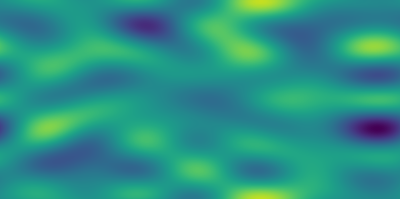
\includegraphics[interpolate=false,width=1.000000in,height=1.000000in]{burgers_rollout_target_0.1-img0.png}}%
\end{pgfscope}%
\begin{pgfscope}%
\pgfsetbuttcap%
\pgfsetroundjoin%
\definecolor{currentfill}{rgb}{0.000000,0.000000,0.000000}%
\pgfsetfillcolor{currentfill}%
\pgfsetlinewidth{0.803000pt}%
\definecolor{currentstroke}{rgb}{0.000000,0.000000,0.000000}%
\pgfsetstrokecolor{currentstroke}%
\pgfsetdash{}{0pt}%
\pgfsys@defobject{currentmarker}{\pgfqpoint{0.000000in}{-0.048611in}}{\pgfqpoint{0.000000in}{0.000000in}}{%
\pgfpathmoveto{\pgfqpoint{0.000000in}{0.000000in}}%
\pgfpathlineto{\pgfqpoint{0.000000in}{-0.048611in}}%
\pgfusepath{stroke,fill}%
}%
\begin{pgfscope}%
\pgfsys@transformshift{0.726837in}{0.517039in}%
\pgfsys@useobject{currentmarker}{}%
\end{pgfscope}%
\end{pgfscope}%
\begin{pgfscope}%
\definecolor{textcolor}{rgb}{0.000000,0.000000,0.000000}%
\pgfsetstrokecolor{textcolor}%
\pgfsetfillcolor{textcolor}%
\pgftext[x=0.726837in,y=0.419816in,,top]{\color{textcolor}\rmfamily\fontsize{12.000000}{14.400000}\selectfont 0}%
\end{pgfscope}%
\begin{pgfscope}%
\pgfsetbuttcap%
\pgfsetroundjoin%
\definecolor{currentfill}{rgb}{0.000000,0.000000,0.000000}%
\pgfsetfillcolor{currentfill}%
\pgfsetlinewidth{0.803000pt}%
\definecolor{currentstroke}{rgb}{0.000000,0.000000,0.000000}%
\pgfsetstrokecolor{currentstroke}%
\pgfsetdash{}{0pt}%
\pgfsys@defobject{currentmarker}{\pgfqpoint{0.000000in}{-0.048611in}}{\pgfqpoint{0.000000in}{0.000000in}}{%
\pgfpathmoveto{\pgfqpoint{0.000000in}{0.000000in}}%
\pgfpathlineto{\pgfqpoint{0.000000in}{-0.048611in}}%
\pgfusepath{stroke,fill}%
}%
\begin{pgfscope}%
\pgfsys@transformshift{1.570762in}{0.517039in}%
\pgfsys@useobject{currentmarker}{}%
\end{pgfscope}%
\end{pgfscope}%
\begin{pgfscope}%
\definecolor{textcolor}{rgb}{0.000000,0.000000,0.000000}%
\pgfsetstrokecolor{textcolor}%
\pgfsetfillcolor{textcolor}%
\pgftext[x=1.570762in,y=0.419816in,,top]{\color{textcolor}\rmfamily\fontsize{12.000000}{14.400000}\selectfont 1}%
\end{pgfscope}%
\begin{pgfscope}%
\pgfsetbuttcap%
\pgfsetroundjoin%
\definecolor{currentfill}{rgb}{0.000000,0.000000,0.000000}%
\pgfsetfillcolor{currentfill}%
\pgfsetlinewidth{0.803000pt}%
\definecolor{currentstroke}{rgb}{0.000000,0.000000,0.000000}%
\pgfsetstrokecolor{currentstroke}%
\pgfsetdash{}{0pt}%
\pgfsys@defobject{currentmarker}{\pgfqpoint{0.000000in}{-0.048611in}}{\pgfqpoint{0.000000in}{0.000000in}}{%
\pgfpathmoveto{\pgfqpoint{0.000000in}{0.000000in}}%
\pgfpathlineto{\pgfqpoint{0.000000in}{-0.048611in}}%
\pgfusepath{stroke,fill}%
}%
\begin{pgfscope}%
\pgfsys@transformshift{2.414687in}{0.517039in}%
\pgfsys@useobject{currentmarker}{}%
\end{pgfscope}%
\end{pgfscope}%
\begin{pgfscope}%
\definecolor{textcolor}{rgb}{0.000000,0.000000,0.000000}%
\pgfsetstrokecolor{textcolor}%
\pgfsetfillcolor{textcolor}%
\pgftext[x=2.414687in,y=0.419816in,,top]{\color{textcolor}\rmfamily\fontsize{12.000000}{14.400000}\selectfont 2}%
\end{pgfscope}%
\begin{pgfscope}%
\definecolor{textcolor}{rgb}{0.000000,0.000000,0.000000}%
\pgfsetstrokecolor{textcolor}%
\pgfsetfillcolor{textcolor}%
\pgftext[x=1.570762in,y=0.202965in,,top]{\color{textcolor}\rmfamily\fontsize{12.000000}{14.400000}\selectfont Space}%
\end{pgfscope}%
\begin{pgfscope}%
\pgfsetbuttcap%
\pgfsetroundjoin%
\definecolor{currentfill}{rgb}{0.000000,0.000000,0.000000}%
\pgfsetfillcolor{currentfill}%
\pgfsetlinewidth{0.803000pt}%
\definecolor{currentstroke}{rgb}{0.000000,0.000000,0.000000}%
\pgfsetstrokecolor{currentstroke}%
\pgfsetdash{}{0pt}%
\pgfsys@defobject{currentmarker}{\pgfqpoint{-0.048611in}{0.000000in}}{\pgfqpoint{-0.000000in}{0.000000in}}{%
\pgfpathmoveto{\pgfqpoint{-0.000000in}{0.000000in}}%
\pgfpathlineto{\pgfqpoint{-0.048611in}{0.000000in}}%
\pgfusepath{stroke,fill}%
}%
\begin{pgfscope}%
\pgfsys@transformshift{0.726837in}{0.517039in}%
\pgfsys@useobject{currentmarker}{}%
\end{pgfscope}%
\end{pgfscope}%
\begin{pgfscope}%
\definecolor{textcolor}{rgb}{0.000000,0.000000,0.000000}%
\pgfsetstrokecolor{textcolor}%
\pgfsetfillcolor{textcolor}%
\pgftext[x=0.364559in, y=0.453725in, left, base]{\color{textcolor}\rmfamily\fontsize{12.000000}{14.400000}\selectfont 0.0}%
\end{pgfscope}%
\begin{pgfscope}%
\pgfsetbuttcap%
\pgfsetroundjoin%
\definecolor{currentfill}{rgb}{0.000000,0.000000,0.000000}%
\pgfsetfillcolor{currentfill}%
\pgfsetlinewidth{0.803000pt}%
\definecolor{currentstroke}{rgb}{0.000000,0.000000,0.000000}%
\pgfsetstrokecolor{currentstroke}%
\pgfsetdash{}{0pt}%
\pgfsys@defobject{currentmarker}{\pgfqpoint{-0.048611in}{0.000000in}}{\pgfqpoint{-0.000000in}{0.000000in}}{%
\pgfpathmoveto{\pgfqpoint{-0.000000in}{0.000000in}}%
\pgfpathlineto{\pgfqpoint{-0.048611in}{0.000000in}}%
\pgfusepath{stroke,fill}%
}%
\begin{pgfscope}%
\pgfsys@transformshift{0.726837in}{0.861533in}%
\pgfsys@useobject{currentmarker}{}%
\end{pgfscope}%
\end{pgfscope}%
\begin{pgfscope}%
\definecolor{textcolor}{rgb}{0.000000,0.000000,0.000000}%
\pgfsetstrokecolor{textcolor}%
\pgfsetfillcolor{textcolor}%
\pgftext[x=0.364559in, y=0.798219in, left, base]{\color{textcolor}\rmfamily\fontsize{12.000000}{14.400000}\selectfont 2.5}%
\end{pgfscope}%
\begin{pgfscope}%
\pgfsetbuttcap%
\pgfsetroundjoin%
\definecolor{currentfill}{rgb}{0.000000,0.000000,0.000000}%
\pgfsetfillcolor{currentfill}%
\pgfsetlinewidth{0.803000pt}%
\definecolor{currentstroke}{rgb}{0.000000,0.000000,0.000000}%
\pgfsetstrokecolor{currentstroke}%
\pgfsetdash{}{0pt}%
\pgfsys@defobject{currentmarker}{\pgfqpoint{-0.048611in}{0.000000in}}{\pgfqpoint{-0.000000in}{0.000000in}}{%
\pgfpathmoveto{\pgfqpoint{-0.000000in}{0.000000in}}%
\pgfpathlineto{\pgfqpoint{-0.048611in}{0.000000in}}%
\pgfusepath{stroke,fill}%
}%
\begin{pgfscope}%
\pgfsys@transformshift{0.726837in}{1.206027in}%
\pgfsys@useobject{currentmarker}{}%
\end{pgfscope}%
\end{pgfscope}%
\begin{pgfscope}%
\definecolor{textcolor}{rgb}{0.000000,0.000000,0.000000}%
\pgfsetstrokecolor{textcolor}%
\pgfsetfillcolor{textcolor}%
\pgftext[x=0.364559in, y=1.142714in, left, base]{\color{textcolor}\rmfamily\fontsize{12.000000}{14.400000}\selectfont 5.0}%
\end{pgfscope}%
\begin{pgfscope}%
\pgfsetbuttcap%
\pgfsetroundjoin%
\definecolor{currentfill}{rgb}{0.000000,0.000000,0.000000}%
\pgfsetfillcolor{currentfill}%
\pgfsetlinewidth{0.803000pt}%
\definecolor{currentstroke}{rgb}{0.000000,0.000000,0.000000}%
\pgfsetstrokecolor{currentstroke}%
\pgfsetdash{}{0pt}%
\pgfsys@defobject{currentmarker}{\pgfqpoint{-0.048611in}{0.000000in}}{\pgfqpoint{-0.000000in}{0.000000in}}{%
\pgfpathmoveto{\pgfqpoint{-0.000000in}{0.000000in}}%
\pgfpathlineto{\pgfqpoint{-0.048611in}{0.000000in}}%
\pgfusepath{stroke,fill}%
}%
\begin{pgfscope}%
\pgfsys@transformshift{0.726837in}{1.550522in}%
\pgfsys@useobject{currentmarker}{}%
\end{pgfscope}%
\end{pgfscope}%
\begin{pgfscope}%
\definecolor{textcolor}{rgb}{0.000000,0.000000,0.000000}%
\pgfsetstrokecolor{textcolor}%
\pgfsetfillcolor{textcolor}%
\pgftext[x=0.364559in, y=1.487208in, left, base]{\color{textcolor}\rmfamily\fontsize{12.000000}{14.400000}\selectfont 7.5}%
\end{pgfscope}%
\begin{pgfscope}%
\pgfsetbuttcap%
\pgfsetroundjoin%
\definecolor{currentfill}{rgb}{0.000000,0.000000,0.000000}%
\pgfsetfillcolor{currentfill}%
\pgfsetlinewidth{0.803000pt}%
\definecolor{currentstroke}{rgb}{0.000000,0.000000,0.000000}%
\pgfsetstrokecolor{currentstroke}%
\pgfsetdash{}{0pt}%
\pgfsys@defobject{currentmarker}{\pgfqpoint{-0.048611in}{0.000000in}}{\pgfqpoint{-0.000000in}{0.000000in}}{%
\pgfpathmoveto{\pgfqpoint{-0.000000in}{0.000000in}}%
\pgfpathlineto{\pgfqpoint{-0.048611in}{0.000000in}}%
\pgfusepath{stroke,fill}%
}%
\begin{pgfscope}%
\pgfsys@transformshift{0.726837in}{1.895016in}%
\pgfsys@useobject{currentmarker}{}%
\end{pgfscope}%
\end{pgfscope}%
\begin{pgfscope}%
\definecolor{textcolor}{rgb}{0.000000,0.000000,0.000000}%
\pgfsetstrokecolor{textcolor}%
\pgfsetfillcolor{textcolor}%
\pgftext[x=0.258521in, y=1.831702in, left, base]{\color{textcolor}\rmfamily\fontsize{12.000000}{14.400000}\selectfont 10.0}%
\end{pgfscope}%
\begin{pgfscope}%
\definecolor{textcolor}{rgb}{0.000000,0.000000,0.000000}%
\pgfsetstrokecolor{textcolor}%
\pgfsetfillcolor{textcolor}%
\pgftext[x=0.202965in,y=1.206027in,,bottom,rotate=90.000000]{\color{textcolor}\rmfamily\fontsize{12.000000}{14.400000}\selectfont Time}%
\end{pgfscope}%
\begin{pgfscope}%
\pgfsetrectcap%
\pgfsetmiterjoin%
\pgfsetlinewidth{0.803000pt}%
\definecolor{currentstroke}{rgb}{0.000000,0.000000,0.000000}%
\pgfsetstrokecolor{currentstroke}%
\pgfsetdash{}{0pt}%
\pgfpathmoveto{\pgfqpoint{0.726837in}{0.517039in}}%
\pgfpathlineto{\pgfqpoint{0.726837in}{1.895016in}}%
\pgfusepath{stroke}%
\end{pgfscope}%
\begin{pgfscope}%
\pgfsetrectcap%
\pgfsetmiterjoin%
\pgfsetlinewidth{0.803000pt}%
\definecolor{currentstroke}{rgb}{0.000000,0.000000,0.000000}%
\pgfsetstrokecolor{currentstroke}%
\pgfsetdash{}{0pt}%
\pgfpathmoveto{\pgfqpoint{2.414687in}{0.517039in}}%
\pgfpathlineto{\pgfqpoint{2.414687in}{1.895016in}}%
\pgfusepath{stroke}%
\end{pgfscope}%
\begin{pgfscope}%
\pgfsetrectcap%
\pgfsetmiterjoin%
\pgfsetlinewidth{0.803000pt}%
\definecolor{currentstroke}{rgb}{0.000000,0.000000,0.000000}%
\pgfsetstrokecolor{currentstroke}%
\pgfsetdash{}{0pt}%
\pgfpathmoveto{\pgfqpoint{0.726837in}{0.517039in}}%
\pgfpathlineto{\pgfqpoint{2.414687in}{0.517039in}}%
\pgfusepath{stroke}%
\end{pgfscope}%
\begin{pgfscope}%
\pgfsetrectcap%
\pgfsetmiterjoin%
\pgfsetlinewidth{0.803000pt}%
\definecolor{currentstroke}{rgb}{0.000000,0.000000,0.000000}%
\pgfsetstrokecolor{currentstroke}%
\pgfsetdash{}{0pt}%
\pgfpathmoveto{\pgfqpoint{0.726837in}{1.895016in}}%
\pgfpathlineto{\pgfqpoint{2.414687in}{1.895016in}}%
\pgfusepath{stroke}%
\end{pgfscope}%
\begin{pgfscope}%
\pgfsetbuttcap%
\pgfsetmiterjoin%
\pgfsetlinewidth{0.000000pt}%
\definecolor{currentstroke}{rgb}{0.000000,0.000000,0.000000}%
\pgfsetstrokecolor{currentstroke}%
\pgfsetstrokeopacity{0.000000}%
\pgfsetdash{}{0pt}%
\pgfpathmoveto{\pgfqpoint{2.552099in}{0.517039in}}%
\pgfpathlineto{\pgfqpoint{2.620998in}{0.517039in}}%
\pgfpathlineto{\pgfqpoint{2.620998in}{1.895016in}}%
\pgfpathlineto{\pgfqpoint{2.552099in}{1.895016in}}%
\pgfpathlineto{\pgfqpoint{2.552099in}{0.517039in}}%
\pgfpathclose%
\pgfusepath{}%
\end{pgfscope}%
\begin{pgfscope}%
\pgfsys@transformshift{2.550000in}{0.520000in}%
\pgftext[left,bottom]{
\includegraphics[interpolate=true,width=0.070000in,height=1.380000in]{burgers_rollout_target_0.1-img1.png}}%
\end{pgfscope}%
\begin{pgfscope}%
\pgfsetbuttcap%
\pgfsetroundjoin%
\definecolor{currentfill}{rgb}{0.000000,0.000000,0.000000}%
\pgfsetfillcolor{currentfill}%
\pgfsetlinewidth{0.803000pt}%
\definecolor{currentstroke}{rgb}{0.000000,0.000000,0.000000}%
\pgfsetstrokecolor{currentstroke}%
\pgfsetdash{}{0pt}%
\pgfsys@defobject{currentmarker}{\pgfqpoint{0.000000in}{0.000000in}}{\pgfqpoint{0.048611in}{0.000000in}}{%
\pgfpathmoveto{\pgfqpoint{0.000000in}{0.000000in}}%
\pgfpathlineto{\pgfqpoint{0.048611in}{0.000000in}}%
\pgfusepath{stroke,fill}%
}%
\begin{pgfscope}%
\pgfsys@transformshift{2.620998in}{0.588723in}%
\pgfsys@useobject{currentmarker}{}%
\end{pgfscope}%
\end{pgfscope}%
\begin{pgfscope}%
\definecolor{textcolor}{rgb}{0.000000,0.000000,0.000000}%
\pgfsetstrokecolor{textcolor}%
\pgfsetfillcolor{textcolor}%
\pgftext[x=2.718220in, y=0.525410in, left, base]{\color{textcolor}\rmfamily\fontsize{12.000000}{14.400000}\selectfont \ensuremath{-}1}%
\end{pgfscope}%
\begin{pgfscope}%
\pgfsetbuttcap%
\pgfsetroundjoin%
\definecolor{currentfill}{rgb}{0.000000,0.000000,0.000000}%
\pgfsetfillcolor{currentfill}%
\pgfsetlinewidth{0.803000pt}%
\definecolor{currentstroke}{rgb}{0.000000,0.000000,0.000000}%
\pgfsetstrokecolor{currentstroke}%
\pgfsetdash{}{0pt}%
\pgfsys@defobject{currentmarker}{\pgfqpoint{0.000000in}{0.000000in}}{\pgfqpoint{0.048611in}{0.000000in}}{%
\pgfpathmoveto{\pgfqpoint{0.000000in}{0.000000in}}%
\pgfpathlineto{\pgfqpoint{0.048611in}{0.000000in}}%
\pgfusepath{stroke,fill}%
}%
\begin{pgfscope}%
\pgfsys@transformshift{2.620998in}{1.206027in}%
\pgfsys@useobject{currentmarker}{}%
\end{pgfscope}%
\end{pgfscope}%
\begin{pgfscope}%
\definecolor{textcolor}{rgb}{0.000000,0.000000,0.000000}%
\pgfsetstrokecolor{textcolor}%
\pgfsetfillcolor{textcolor}%
\pgftext[x=2.718220in, y=1.142714in, left, base]{\color{textcolor}\rmfamily\fontsize{12.000000}{14.400000}\selectfont 0}%
\end{pgfscope}%
\begin{pgfscope}%
\pgfsetbuttcap%
\pgfsetroundjoin%
\definecolor{currentfill}{rgb}{0.000000,0.000000,0.000000}%
\pgfsetfillcolor{currentfill}%
\pgfsetlinewidth{0.803000pt}%
\definecolor{currentstroke}{rgb}{0.000000,0.000000,0.000000}%
\pgfsetstrokecolor{currentstroke}%
\pgfsetdash{}{0pt}%
\pgfsys@defobject{currentmarker}{\pgfqpoint{0.000000in}{0.000000in}}{\pgfqpoint{0.048611in}{0.000000in}}{%
\pgfpathmoveto{\pgfqpoint{0.000000in}{0.000000in}}%
\pgfpathlineto{\pgfqpoint{0.048611in}{0.000000in}}%
\pgfusepath{stroke,fill}%
}%
\begin{pgfscope}%
\pgfsys@transformshift{2.620998in}{1.823331in}%
\pgfsys@useobject{currentmarker}{}%
\end{pgfscope}%
\end{pgfscope}%
\begin{pgfscope}%
\definecolor{textcolor}{rgb}{0.000000,0.000000,0.000000}%
\pgfsetstrokecolor{textcolor}%
\pgfsetfillcolor{textcolor}%
\pgftext[x=2.718220in, y=1.760018in, left, base]{\color{textcolor}\rmfamily\fontsize{12.000000}{14.400000}\selectfont 1}%
\end{pgfscope}%
\begin{pgfscope}%
\pgfsetrectcap%
\pgfsetmiterjoin%
\pgfsetlinewidth{0.803000pt}%
\definecolor{currentstroke}{rgb}{0.000000,0.000000,0.000000}%
\pgfsetstrokecolor{currentstroke}%
\pgfsetdash{}{0pt}%
\pgfpathmoveto{\pgfqpoint{2.552099in}{0.517039in}}%
\pgfpathlineto{\pgfqpoint{2.586548in}{0.517039in}}%
\pgfpathlineto{\pgfqpoint{2.620998in}{0.517039in}}%
\pgfpathlineto{\pgfqpoint{2.620998in}{1.895016in}}%
\pgfpathlineto{\pgfqpoint{2.586548in}{1.895016in}}%
\pgfpathlineto{\pgfqpoint{2.552099in}{1.895016in}}%
\pgfpathlineto{\pgfqpoint{2.552099in}{0.517039in}}%
\pgfpathclose%
\pgfusepath{stroke}%
\end{pgfscope}%
\end{pgfpicture}%
\makeatother%
\endgroup%

      \end{adjustbox}
      \caption{The target for \(\nu=0.1\)}\label{fig:sc2_rollout_target_0.1}
    \end{subfigure}
    \begin{subfigure}{0.33\linewidth}
      \begin{adjustbox}{width=\linewidth}
        \begingroup%
\makeatletter%
\begin{pgfpicture}%
\pgfpathrectangle{\pgfpointorigin}{\pgfqpoint{3.000000in}{2.000000in}}%
\pgfusepath{use as bounding box, clip}%
\begin{pgfscope}%
\pgfsetbuttcap%
\pgfsetmiterjoin%
\pgfsetlinewidth{0.000000pt}%
\definecolor{currentstroke}{rgb}{0.000000,0.000000,0.000000}%
\pgfsetstrokecolor{currentstroke}%
\pgfsetstrokeopacity{0.000000}%
\pgfsetdash{}{0pt}%
\pgfpathmoveto{\pgfqpoint{0.000000in}{0.000000in}}%
\pgfpathlineto{\pgfqpoint{3.000000in}{0.000000in}}%
\pgfpathlineto{\pgfqpoint{3.000000in}{2.000000in}}%
\pgfpathlineto{\pgfqpoint{0.000000in}{2.000000in}}%
\pgfpathlineto{\pgfqpoint{0.000000in}{0.000000in}}%
\pgfpathclose%
\pgfusepath{}%
\end{pgfscope}%
\begin{pgfscope}%
\pgfsetbuttcap%
\pgfsetmiterjoin%
\pgfsetlinewidth{0.000000pt}%
\definecolor{currentstroke}{rgb}{0.000000,0.000000,0.000000}%
\pgfsetstrokecolor{currentstroke}%
\pgfsetstrokeopacity{0.000000}%
\pgfsetdash{}{0pt}%
\pgfpathmoveto{\pgfqpoint{0.726837in}{0.517039in}}%
\pgfpathlineto{\pgfqpoint{2.414687in}{0.517039in}}%
\pgfpathlineto{\pgfqpoint{2.414687in}{1.895016in}}%
\pgfpathlineto{\pgfqpoint{0.726837in}{1.895016in}}%
\pgfpathlineto{\pgfqpoint{0.726837in}{0.517039in}}%
\pgfpathclose%
\pgfusepath{}%
\end{pgfscope}%
\begin{pgfscope}%
\pgfpathrectangle{\pgfqpoint{0.726837in}{0.517039in}}{\pgfqpoint{1.687850in}{1.377978in}}%
\pgfusepath{clip}%
\pgfsys@transformcm{1.687850}{0.000000}{0.000000}{1.377978}{0.726837in}{0.517039in}%
\pgftext[left,bottom]{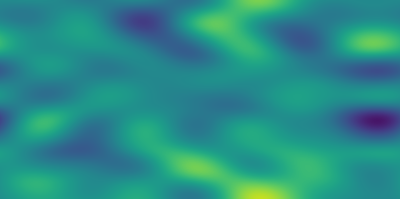
\includegraphics[interpolate=false,width=1.000000in,height=1.000000in]{burgers_rollout_pred_0.1-img0.png}}%
\end{pgfscope}%
\begin{pgfscope}%
\pgfsetbuttcap%
\pgfsetroundjoin%
\definecolor{currentfill}{rgb}{0.000000,0.000000,0.000000}%
\pgfsetfillcolor{currentfill}%
\pgfsetlinewidth{0.803000pt}%
\definecolor{currentstroke}{rgb}{0.000000,0.000000,0.000000}%
\pgfsetstrokecolor{currentstroke}%
\pgfsetdash{}{0pt}%
\pgfsys@defobject{currentmarker}{\pgfqpoint{0.000000in}{-0.048611in}}{\pgfqpoint{0.000000in}{0.000000in}}{%
\pgfpathmoveto{\pgfqpoint{0.000000in}{0.000000in}}%
\pgfpathlineto{\pgfqpoint{0.000000in}{-0.048611in}}%
\pgfusepath{stroke,fill}%
}%
\begin{pgfscope}%
\pgfsys@transformshift{0.726837in}{0.517039in}%
\pgfsys@useobject{currentmarker}{}%
\end{pgfscope}%
\end{pgfscope}%
\begin{pgfscope}%
\definecolor{textcolor}{rgb}{0.000000,0.000000,0.000000}%
\pgfsetstrokecolor{textcolor}%
\pgfsetfillcolor{textcolor}%
\pgftext[x=0.726837in,y=0.419816in,,top]{\color{textcolor}\rmfamily\fontsize{12.000000}{14.400000}\selectfont 0}%
\end{pgfscope}%
\begin{pgfscope}%
\pgfsetbuttcap%
\pgfsetroundjoin%
\definecolor{currentfill}{rgb}{0.000000,0.000000,0.000000}%
\pgfsetfillcolor{currentfill}%
\pgfsetlinewidth{0.803000pt}%
\definecolor{currentstroke}{rgb}{0.000000,0.000000,0.000000}%
\pgfsetstrokecolor{currentstroke}%
\pgfsetdash{}{0pt}%
\pgfsys@defobject{currentmarker}{\pgfqpoint{0.000000in}{-0.048611in}}{\pgfqpoint{0.000000in}{0.000000in}}{%
\pgfpathmoveto{\pgfqpoint{0.000000in}{0.000000in}}%
\pgfpathlineto{\pgfqpoint{0.000000in}{-0.048611in}}%
\pgfusepath{stroke,fill}%
}%
\begin{pgfscope}%
\pgfsys@transformshift{1.570762in}{0.517039in}%
\pgfsys@useobject{currentmarker}{}%
\end{pgfscope}%
\end{pgfscope}%
\begin{pgfscope}%
\definecolor{textcolor}{rgb}{0.000000,0.000000,0.000000}%
\pgfsetstrokecolor{textcolor}%
\pgfsetfillcolor{textcolor}%
\pgftext[x=1.570762in,y=0.419816in,,top]{\color{textcolor}\rmfamily\fontsize{12.000000}{14.400000}\selectfont 1}%
\end{pgfscope}%
\begin{pgfscope}%
\pgfsetbuttcap%
\pgfsetroundjoin%
\definecolor{currentfill}{rgb}{0.000000,0.000000,0.000000}%
\pgfsetfillcolor{currentfill}%
\pgfsetlinewidth{0.803000pt}%
\definecolor{currentstroke}{rgb}{0.000000,0.000000,0.000000}%
\pgfsetstrokecolor{currentstroke}%
\pgfsetdash{}{0pt}%
\pgfsys@defobject{currentmarker}{\pgfqpoint{0.000000in}{-0.048611in}}{\pgfqpoint{0.000000in}{0.000000in}}{%
\pgfpathmoveto{\pgfqpoint{0.000000in}{0.000000in}}%
\pgfpathlineto{\pgfqpoint{0.000000in}{-0.048611in}}%
\pgfusepath{stroke,fill}%
}%
\begin{pgfscope}%
\pgfsys@transformshift{2.414687in}{0.517039in}%
\pgfsys@useobject{currentmarker}{}%
\end{pgfscope}%
\end{pgfscope}%
\begin{pgfscope}%
\definecolor{textcolor}{rgb}{0.000000,0.000000,0.000000}%
\pgfsetstrokecolor{textcolor}%
\pgfsetfillcolor{textcolor}%
\pgftext[x=2.414687in,y=0.419816in,,top]{\color{textcolor}\rmfamily\fontsize{12.000000}{14.400000}\selectfont 2}%
\end{pgfscope}%
\begin{pgfscope}%
\definecolor{textcolor}{rgb}{0.000000,0.000000,0.000000}%
\pgfsetstrokecolor{textcolor}%
\pgfsetfillcolor{textcolor}%
\pgftext[x=1.570762in,y=0.202965in,,top]{\color{textcolor}\rmfamily\fontsize{12.000000}{14.400000}\selectfont Space}%
\end{pgfscope}%
\begin{pgfscope}%
\pgfsetbuttcap%
\pgfsetroundjoin%
\definecolor{currentfill}{rgb}{0.000000,0.000000,0.000000}%
\pgfsetfillcolor{currentfill}%
\pgfsetlinewidth{0.803000pt}%
\definecolor{currentstroke}{rgb}{0.000000,0.000000,0.000000}%
\pgfsetstrokecolor{currentstroke}%
\pgfsetdash{}{0pt}%
\pgfsys@defobject{currentmarker}{\pgfqpoint{-0.048611in}{0.000000in}}{\pgfqpoint{-0.000000in}{0.000000in}}{%
\pgfpathmoveto{\pgfqpoint{-0.000000in}{0.000000in}}%
\pgfpathlineto{\pgfqpoint{-0.048611in}{0.000000in}}%
\pgfusepath{stroke,fill}%
}%
\begin{pgfscope}%
\pgfsys@transformshift{0.726837in}{0.517039in}%
\pgfsys@useobject{currentmarker}{}%
\end{pgfscope}%
\end{pgfscope}%
\begin{pgfscope}%
\definecolor{textcolor}{rgb}{0.000000,0.000000,0.000000}%
\pgfsetstrokecolor{textcolor}%
\pgfsetfillcolor{textcolor}%
\pgftext[x=0.364559in, y=0.453725in, left, base]{\color{textcolor}\rmfamily\fontsize{12.000000}{14.400000}\selectfont 0.0}%
\end{pgfscope}%
\begin{pgfscope}%
\pgfsetbuttcap%
\pgfsetroundjoin%
\definecolor{currentfill}{rgb}{0.000000,0.000000,0.000000}%
\pgfsetfillcolor{currentfill}%
\pgfsetlinewidth{0.803000pt}%
\definecolor{currentstroke}{rgb}{0.000000,0.000000,0.000000}%
\pgfsetstrokecolor{currentstroke}%
\pgfsetdash{}{0pt}%
\pgfsys@defobject{currentmarker}{\pgfqpoint{-0.048611in}{0.000000in}}{\pgfqpoint{-0.000000in}{0.000000in}}{%
\pgfpathmoveto{\pgfqpoint{-0.000000in}{0.000000in}}%
\pgfpathlineto{\pgfqpoint{-0.048611in}{0.000000in}}%
\pgfusepath{stroke,fill}%
}%
\begin{pgfscope}%
\pgfsys@transformshift{0.726837in}{0.861533in}%
\pgfsys@useobject{currentmarker}{}%
\end{pgfscope}%
\end{pgfscope}%
\begin{pgfscope}%
\definecolor{textcolor}{rgb}{0.000000,0.000000,0.000000}%
\pgfsetstrokecolor{textcolor}%
\pgfsetfillcolor{textcolor}%
\pgftext[x=0.364559in, y=0.798219in, left, base]{\color{textcolor}\rmfamily\fontsize{12.000000}{14.400000}\selectfont 2.5}%
\end{pgfscope}%
\begin{pgfscope}%
\pgfsetbuttcap%
\pgfsetroundjoin%
\definecolor{currentfill}{rgb}{0.000000,0.000000,0.000000}%
\pgfsetfillcolor{currentfill}%
\pgfsetlinewidth{0.803000pt}%
\definecolor{currentstroke}{rgb}{0.000000,0.000000,0.000000}%
\pgfsetstrokecolor{currentstroke}%
\pgfsetdash{}{0pt}%
\pgfsys@defobject{currentmarker}{\pgfqpoint{-0.048611in}{0.000000in}}{\pgfqpoint{-0.000000in}{0.000000in}}{%
\pgfpathmoveto{\pgfqpoint{-0.000000in}{0.000000in}}%
\pgfpathlineto{\pgfqpoint{-0.048611in}{0.000000in}}%
\pgfusepath{stroke,fill}%
}%
\begin{pgfscope}%
\pgfsys@transformshift{0.726837in}{1.206027in}%
\pgfsys@useobject{currentmarker}{}%
\end{pgfscope}%
\end{pgfscope}%
\begin{pgfscope}%
\definecolor{textcolor}{rgb}{0.000000,0.000000,0.000000}%
\pgfsetstrokecolor{textcolor}%
\pgfsetfillcolor{textcolor}%
\pgftext[x=0.364559in, y=1.142714in, left, base]{\color{textcolor}\rmfamily\fontsize{12.000000}{14.400000}\selectfont 5.0}%
\end{pgfscope}%
\begin{pgfscope}%
\pgfsetbuttcap%
\pgfsetroundjoin%
\definecolor{currentfill}{rgb}{0.000000,0.000000,0.000000}%
\pgfsetfillcolor{currentfill}%
\pgfsetlinewidth{0.803000pt}%
\definecolor{currentstroke}{rgb}{0.000000,0.000000,0.000000}%
\pgfsetstrokecolor{currentstroke}%
\pgfsetdash{}{0pt}%
\pgfsys@defobject{currentmarker}{\pgfqpoint{-0.048611in}{0.000000in}}{\pgfqpoint{-0.000000in}{0.000000in}}{%
\pgfpathmoveto{\pgfqpoint{-0.000000in}{0.000000in}}%
\pgfpathlineto{\pgfqpoint{-0.048611in}{0.000000in}}%
\pgfusepath{stroke,fill}%
}%
\begin{pgfscope}%
\pgfsys@transformshift{0.726837in}{1.550522in}%
\pgfsys@useobject{currentmarker}{}%
\end{pgfscope}%
\end{pgfscope}%
\begin{pgfscope}%
\definecolor{textcolor}{rgb}{0.000000,0.000000,0.000000}%
\pgfsetstrokecolor{textcolor}%
\pgfsetfillcolor{textcolor}%
\pgftext[x=0.364559in, y=1.487208in, left, base]{\color{textcolor}\rmfamily\fontsize{12.000000}{14.400000}\selectfont 7.5}%
\end{pgfscope}%
\begin{pgfscope}%
\pgfsetbuttcap%
\pgfsetroundjoin%
\definecolor{currentfill}{rgb}{0.000000,0.000000,0.000000}%
\pgfsetfillcolor{currentfill}%
\pgfsetlinewidth{0.803000pt}%
\definecolor{currentstroke}{rgb}{0.000000,0.000000,0.000000}%
\pgfsetstrokecolor{currentstroke}%
\pgfsetdash{}{0pt}%
\pgfsys@defobject{currentmarker}{\pgfqpoint{-0.048611in}{0.000000in}}{\pgfqpoint{-0.000000in}{0.000000in}}{%
\pgfpathmoveto{\pgfqpoint{-0.000000in}{0.000000in}}%
\pgfpathlineto{\pgfqpoint{-0.048611in}{0.000000in}}%
\pgfusepath{stroke,fill}%
}%
\begin{pgfscope}%
\pgfsys@transformshift{0.726837in}{1.895016in}%
\pgfsys@useobject{currentmarker}{}%
\end{pgfscope}%
\end{pgfscope}%
\begin{pgfscope}%
\definecolor{textcolor}{rgb}{0.000000,0.000000,0.000000}%
\pgfsetstrokecolor{textcolor}%
\pgfsetfillcolor{textcolor}%
\pgftext[x=0.258521in, y=1.831702in, left, base]{\color{textcolor}\rmfamily\fontsize{12.000000}{14.400000}\selectfont 10.0}%
\end{pgfscope}%
\begin{pgfscope}%
\definecolor{textcolor}{rgb}{0.000000,0.000000,0.000000}%
\pgfsetstrokecolor{textcolor}%
\pgfsetfillcolor{textcolor}%
\pgftext[x=0.202965in,y=1.206027in,,bottom,rotate=90.000000]{\color{textcolor}\rmfamily\fontsize{12.000000}{14.400000}\selectfont Time}%
\end{pgfscope}%
\begin{pgfscope}%
\pgfsetrectcap%
\pgfsetmiterjoin%
\pgfsetlinewidth{0.803000pt}%
\definecolor{currentstroke}{rgb}{0.000000,0.000000,0.000000}%
\pgfsetstrokecolor{currentstroke}%
\pgfsetdash{}{0pt}%
\pgfpathmoveto{\pgfqpoint{0.726837in}{0.517039in}}%
\pgfpathlineto{\pgfqpoint{0.726837in}{1.895016in}}%
\pgfusepath{stroke}%
\end{pgfscope}%
\begin{pgfscope}%
\pgfsetrectcap%
\pgfsetmiterjoin%
\pgfsetlinewidth{0.803000pt}%
\definecolor{currentstroke}{rgb}{0.000000,0.000000,0.000000}%
\pgfsetstrokecolor{currentstroke}%
\pgfsetdash{}{0pt}%
\pgfpathmoveto{\pgfqpoint{2.414687in}{0.517039in}}%
\pgfpathlineto{\pgfqpoint{2.414687in}{1.895016in}}%
\pgfusepath{stroke}%
\end{pgfscope}%
\begin{pgfscope}%
\pgfsetrectcap%
\pgfsetmiterjoin%
\pgfsetlinewidth{0.803000pt}%
\definecolor{currentstroke}{rgb}{0.000000,0.000000,0.000000}%
\pgfsetstrokecolor{currentstroke}%
\pgfsetdash{}{0pt}%
\pgfpathmoveto{\pgfqpoint{0.726837in}{0.517039in}}%
\pgfpathlineto{\pgfqpoint{2.414687in}{0.517039in}}%
\pgfusepath{stroke}%
\end{pgfscope}%
\begin{pgfscope}%
\pgfsetrectcap%
\pgfsetmiterjoin%
\pgfsetlinewidth{0.803000pt}%
\definecolor{currentstroke}{rgb}{0.000000,0.000000,0.000000}%
\pgfsetstrokecolor{currentstroke}%
\pgfsetdash{}{0pt}%
\pgfpathmoveto{\pgfqpoint{0.726837in}{1.895016in}}%
\pgfpathlineto{\pgfqpoint{2.414687in}{1.895016in}}%
\pgfusepath{stroke}%
\end{pgfscope}%
\begin{pgfscope}%
\pgfsetbuttcap%
\pgfsetmiterjoin%
\pgfsetlinewidth{0.000000pt}%
\definecolor{currentstroke}{rgb}{0.000000,0.000000,0.000000}%
\pgfsetstrokecolor{currentstroke}%
\pgfsetstrokeopacity{0.000000}%
\pgfsetdash{}{0pt}%
\pgfpathmoveto{\pgfqpoint{2.552099in}{0.517039in}}%
\pgfpathlineto{\pgfqpoint{2.620998in}{0.517039in}}%
\pgfpathlineto{\pgfqpoint{2.620998in}{1.895016in}}%
\pgfpathlineto{\pgfqpoint{2.552099in}{1.895016in}}%
\pgfpathlineto{\pgfqpoint{2.552099in}{0.517039in}}%
\pgfpathclose%
\pgfusepath{}%
\end{pgfscope}%
\begin{pgfscope}%
\pgfsys@transformshift{2.550000in}{0.520000in}%
\pgftext[left,bottom]{
\includegraphics[interpolate=true,width=0.070000in,height=1.380000in]{burgers_rollout_pred_0.1-img1.png}}%
\end{pgfscope}%
\begin{pgfscope}%
\pgfsetbuttcap%
\pgfsetroundjoin%
\definecolor{currentfill}{rgb}{0.000000,0.000000,0.000000}%
\pgfsetfillcolor{currentfill}%
\pgfsetlinewidth{0.803000pt}%
\definecolor{currentstroke}{rgb}{0.000000,0.000000,0.000000}%
\pgfsetstrokecolor{currentstroke}%
\pgfsetdash{}{0pt}%
\pgfsys@defobject{currentmarker}{\pgfqpoint{0.000000in}{0.000000in}}{\pgfqpoint{0.048611in}{0.000000in}}{%
\pgfpathmoveto{\pgfqpoint{0.000000in}{0.000000in}}%
\pgfpathlineto{\pgfqpoint{0.048611in}{0.000000in}}%
\pgfusepath{stroke,fill}%
}%
\begin{pgfscope}%
\pgfsys@transformshift{2.620998in}{0.588723in}%
\pgfsys@useobject{currentmarker}{}%
\end{pgfscope}%
\end{pgfscope}%
\begin{pgfscope}%
\definecolor{textcolor}{rgb}{0.000000,0.000000,0.000000}%
\pgfsetstrokecolor{textcolor}%
\pgfsetfillcolor{textcolor}%
\pgftext[x=2.718220in, y=0.525410in, left, base]{\color{textcolor}\rmfamily\fontsize{12.000000}{14.400000}\selectfont \ensuremath{-}1}%
\end{pgfscope}%
\begin{pgfscope}%
\pgfsetbuttcap%
\pgfsetroundjoin%
\definecolor{currentfill}{rgb}{0.000000,0.000000,0.000000}%
\pgfsetfillcolor{currentfill}%
\pgfsetlinewidth{0.803000pt}%
\definecolor{currentstroke}{rgb}{0.000000,0.000000,0.000000}%
\pgfsetstrokecolor{currentstroke}%
\pgfsetdash{}{0pt}%
\pgfsys@defobject{currentmarker}{\pgfqpoint{0.000000in}{0.000000in}}{\pgfqpoint{0.048611in}{0.000000in}}{%
\pgfpathmoveto{\pgfqpoint{0.000000in}{0.000000in}}%
\pgfpathlineto{\pgfqpoint{0.048611in}{0.000000in}}%
\pgfusepath{stroke,fill}%
}%
\begin{pgfscope}%
\pgfsys@transformshift{2.620998in}{1.206027in}%
\pgfsys@useobject{currentmarker}{}%
\end{pgfscope}%
\end{pgfscope}%
\begin{pgfscope}%
\definecolor{textcolor}{rgb}{0.000000,0.000000,0.000000}%
\pgfsetstrokecolor{textcolor}%
\pgfsetfillcolor{textcolor}%
\pgftext[x=2.718220in, y=1.142714in, left, base]{\color{textcolor}\rmfamily\fontsize{12.000000}{14.400000}\selectfont 0}%
\end{pgfscope}%
\begin{pgfscope}%
\pgfsetbuttcap%
\pgfsetroundjoin%
\definecolor{currentfill}{rgb}{0.000000,0.000000,0.000000}%
\pgfsetfillcolor{currentfill}%
\pgfsetlinewidth{0.803000pt}%
\definecolor{currentstroke}{rgb}{0.000000,0.000000,0.000000}%
\pgfsetstrokecolor{currentstroke}%
\pgfsetdash{}{0pt}%
\pgfsys@defobject{currentmarker}{\pgfqpoint{0.000000in}{0.000000in}}{\pgfqpoint{0.048611in}{0.000000in}}{%
\pgfpathmoveto{\pgfqpoint{0.000000in}{0.000000in}}%
\pgfpathlineto{\pgfqpoint{0.048611in}{0.000000in}}%
\pgfusepath{stroke,fill}%
}%
\begin{pgfscope}%
\pgfsys@transformshift{2.620998in}{1.823331in}%
\pgfsys@useobject{currentmarker}{}%
\end{pgfscope}%
\end{pgfscope}%
\begin{pgfscope}%
\definecolor{textcolor}{rgb}{0.000000,0.000000,0.000000}%
\pgfsetstrokecolor{textcolor}%
\pgfsetfillcolor{textcolor}%
\pgftext[x=2.718220in, y=1.760018in, left, base]{\color{textcolor}\rmfamily\fontsize{12.000000}{14.400000}\selectfont 1}%
\end{pgfscope}%
\begin{pgfscope}%
\pgfsetrectcap%
\pgfsetmiterjoin%
\pgfsetlinewidth{0.803000pt}%
\definecolor{currentstroke}{rgb}{0.000000,0.000000,0.000000}%
\pgfsetstrokecolor{currentstroke}%
\pgfsetdash{}{0pt}%
\pgfpathmoveto{\pgfqpoint{2.552099in}{0.517039in}}%
\pgfpathlineto{\pgfqpoint{2.586548in}{0.517039in}}%
\pgfpathlineto{\pgfqpoint{2.620998in}{0.517039in}}%
\pgfpathlineto{\pgfqpoint{2.620998in}{1.895016in}}%
\pgfpathlineto{\pgfqpoint{2.586548in}{1.895016in}}%
\pgfpathlineto{\pgfqpoint{2.552099in}{1.895016in}}%
\pgfpathlineto{\pgfqpoint{2.552099in}{0.517039in}}%
\pgfpathclose%
\pgfusepath{stroke}%
\end{pgfscope}%
\end{pgfpicture}%
\makeatother%
\endgroup%

      \end{adjustbox}
      \caption{The prediction for \(\nu=0.1\)}\label{fig:sc2_rollout_pred_0.1}
    \end{subfigure}
    \begin{subfigure}{0.32\linewidth}
      \begin{adjustbox}{width=\linewidth}
        \begingroup%
\makeatletter%
\begin{pgfpicture}%
\pgfpathrectangle{\pgfpointorigin}{\pgfqpoint{3.000000in}{2.000000in}}%
\pgfusepath{use as bounding box, clip}%
\begin{pgfscope}%
\pgfsetbuttcap%
\pgfsetmiterjoin%
\pgfsetlinewidth{0.000000pt}%
\definecolor{currentstroke}{rgb}{0.000000,0.000000,0.000000}%
\pgfsetstrokecolor{currentstroke}%
\pgfsetstrokeopacity{0.000000}%
\pgfsetdash{}{0pt}%
\pgfpathmoveto{\pgfqpoint{0.000000in}{0.000000in}}%
\pgfpathlineto{\pgfqpoint{3.000000in}{0.000000in}}%
\pgfpathlineto{\pgfqpoint{3.000000in}{2.000000in}}%
\pgfpathlineto{\pgfqpoint{0.000000in}{2.000000in}}%
\pgfpathlineto{\pgfqpoint{0.000000in}{0.000000in}}%
\pgfpathclose%
\pgfusepath{}%
\end{pgfscope}%
\begin{pgfscope}%
\pgfsetbuttcap%
\pgfsetmiterjoin%
\pgfsetlinewidth{0.000000pt}%
\definecolor{currentstroke}{rgb}{0.000000,0.000000,0.000000}%
\pgfsetstrokecolor{currentstroke}%
\pgfsetstrokeopacity{0.000000}%
\pgfsetdash{}{0pt}%
\pgfpathmoveto{\pgfqpoint{0.726837in}{0.517039in}}%
\pgfpathlineto{\pgfqpoint{2.414687in}{0.517039in}}%
\pgfpathlineto{\pgfqpoint{2.414687in}{1.895016in}}%
\pgfpathlineto{\pgfqpoint{0.726837in}{1.895016in}}%
\pgfpathlineto{\pgfqpoint{0.726837in}{0.517039in}}%
\pgfpathclose%
\pgfusepath{}%
\end{pgfscope}%
\begin{pgfscope}%
\pgfpathrectangle{\pgfqpoint{0.726837in}{0.517039in}}{\pgfqpoint{1.687850in}{1.377978in}}%
\pgfusepath{clip}%
\pgfsys@transformcm{1.687850}{0.000000}{0.000000}{1.377978}{0.726837in}{0.517039in}%
\pgftext[left,bottom]{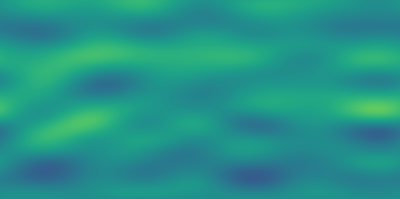
\includegraphics[interpolate=false,width=1.000000in,height=1.000000in]{burgers_rollout_diff_0.1-img0.png}}%
\end{pgfscope}%
\begin{pgfscope}%
\pgfsetbuttcap%
\pgfsetroundjoin%
\definecolor{currentfill}{rgb}{0.000000,0.000000,0.000000}%
\pgfsetfillcolor{currentfill}%
\pgfsetlinewidth{0.803000pt}%
\definecolor{currentstroke}{rgb}{0.000000,0.000000,0.000000}%
\pgfsetstrokecolor{currentstroke}%
\pgfsetdash{}{0pt}%
\pgfsys@defobject{currentmarker}{\pgfqpoint{0.000000in}{-0.048611in}}{\pgfqpoint{0.000000in}{0.000000in}}{%
\pgfpathmoveto{\pgfqpoint{0.000000in}{0.000000in}}%
\pgfpathlineto{\pgfqpoint{0.000000in}{-0.048611in}}%
\pgfusepath{stroke,fill}%
}%
\begin{pgfscope}%
\pgfsys@transformshift{0.726837in}{0.517039in}%
\pgfsys@useobject{currentmarker}{}%
\end{pgfscope}%
\end{pgfscope}%
\begin{pgfscope}%
\definecolor{textcolor}{rgb}{0.000000,0.000000,0.000000}%
\pgfsetstrokecolor{textcolor}%
\pgfsetfillcolor{textcolor}%
\pgftext[x=0.726837in,y=0.419816in,,top]{\color{textcolor}\rmfamily\fontsize{12.000000}{14.400000}\selectfont 0}%
\end{pgfscope}%
\begin{pgfscope}%
\pgfsetbuttcap%
\pgfsetroundjoin%
\definecolor{currentfill}{rgb}{0.000000,0.000000,0.000000}%
\pgfsetfillcolor{currentfill}%
\pgfsetlinewidth{0.803000pt}%
\definecolor{currentstroke}{rgb}{0.000000,0.000000,0.000000}%
\pgfsetstrokecolor{currentstroke}%
\pgfsetdash{}{0pt}%
\pgfsys@defobject{currentmarker}{\pgfqpoint{0.000000in}{-0.048611in}}{\pgfqpoint{0.000000in}{0.000000in}}{%
\pgfpathmoveto{\pgfqpoint{0.000000in}{0.000000in}}%
\pgfpathlineto{\pgfqpoint{0.000000in}{-0.048611in}}%
\pgfusepath{stroke,fill}%
}%
\begin{pgfscope}%
\pgfsys@transformshift{1.570762in}{0.517039in}%
\pgfsys@useobject{currentmarker}{}%
\end{pgfscope}%
\end{pgfscope}%
\begin{pgfscope}%
\definecolor{textcolor}{rgb}{0.000000,0.000000,0.000000}%
\pgfsetstrokecolor{textcolor}%
\pgfsetfillcolor{textcolor}%
\pgftext[x=1.570762in,y=0.419816in,,top]{\color{textcolor}\rmfamily\fontsize{12.000000}{14.400000}\selectfont 1}%
\end{pgfscope}%
\begin{pgfscope}%
\pgfsetbuttcap%
\pgfsetroundjoin%
\definecolor{currentfill}{rgb}{0.000000,0.000000,0.000000}%
\pgfsetfillcolor{currentfill}%
\pgfsetlinewidth{0.803000pt}%
\definecolor{currentstroke}{rgb}{0.000000,0.000000,0.000000}%
\pgfsetstrokecolor{currentstroke}%
\pgfsetdash{}{0pt}%
\pgfsys@defobject{currentmarker}{\pgfqpoint{0.000000in}{-0.048611in}}{\pgfqpoint{0.000000in}{0.000000in}}{%
\pgfpathmoveto{\pgfqpoint{0.000000in}{0.000000in}}%
\pgfpathlineto{\pgfqpoint{0.000000in}{-0.048611in}}%
\pgfusepath{stroke,fill}%
}%
\begin{pgfscope}%
\pgfsys@transformshift{2.414687in}{0.517039in}%
\pgfsys@useobject{currentmarker}{}%
\end{pgfscope}%
\end{pgfscope}%
\begin{pgfscope}%
\definecolor{textcolor}{rgb}{0.000000,0.000000,0.000000}%
\pgfsetstrokecolor{textcolor}%
\pgfsetfillcolor{textcolor}%
\pgftext[x=2.414687in,y=0.419816in,,top]{\color{textcolor}\rmfamily\fontsize{12.000000}{14.400000}\selectfont 2}%
\end{pgfscope}%
\begin{pgfscope}%
\definecolor{textcolor}{rgb}{0.000000,0.000000,0.000000}%
\pgfsetstrokecolor{textcolor}%
\pgfsetfillcolor{textcolor}%
\pgftext[x=1.570762in,y=0.202965in,,top]{\color{textcolor}\rmfamily\fontsize{12.000000}{14.400000}\selectfont Space}%
\end{pgfscope}%
\begin{pgfscope}%
\pgfsetbuttcap%
\pgfsetroundjoin%
\definecolor{currentfill}{rgb}{0.000000,0.000000,0.000000}%
\pgfsetfillcolor{currentfill}%
\pgfsetlinewidth{0.803000pt}%
\definecolor{currentstroke}{rgb}{0.000000,0.000000,0.000000}%
\pgfsetstrokecolor{currentstroke}%
\pgfsetdash{}{0pt}%
\pgfsys@defobject{currentmarker}{\pgfqpoint{-0.048611in}{0.000000in}}{\pgfqpoint{-0.000000in}{0.000000in}}{%
\pgfpathmoveto{\pgfqpoint{-0.000000in}{0.000000in}}%
\pgfpathlineto{\pgfqpoint{-0.048611in}{0.000000in}}%
\pgfusepath{stroke,fill}%
}%
\begin{pgfscope}%
\pgfsys@transformshift{0.726837in}{0.517039in}%
\pgfsys@useobject{currentmarker}{}%
\end{pgfscope}%
\end{pgfscope}%
\begin{pgfscope}%
\definecolor{textcolor}{rgb}{0.000000,0.000000,0.000000}%
\pgfsetstrokecolor{textcolor}%
\pgfsetfillcolor{textcolor}%
\pgftext[x=0.364559in, y=0.453725in, left, base]{\color{textcolor}\rmfamily\fontsize{12.000000}{14.400000}\selectfont 0.0}%
\end{pgfscope}%
\begin{pgfscope}%
\pgfsetbuttcap%
\pgfsetroundjoin%
\definecolor{currentfill}{rgb}{0.000000,0.000000,0.000000}%
\pgfsetfillcolor{currentfill}%
\pgfsetlinewidth{0.803000pt}%
\definecolor{currentstroke}{rgb}{0.000000,0.000000,0.000000}%
\pgfsetstrokecolor{currentstroke}%
\pgfsetdash{}{0pt}%
\pgfsys@defobject{currentmarker}{\pgfqpoint{-0.048611in}{0.000000in}}{\pgfqpoint{-0.000000in}{0.000000in}}{%
\pgfpathmoveto{\pgfqpoint{-0.000000in}{0.000000in}}%
\pgfpathlineto{\pgfqpoint{-0.048611in}{0.000000in}}%
\pgfusepath{stroke,fill}%
}%
\begin{pgfscope}%
\pgfsys@transformshift{0.726837in}{0.861533in}%
\pgfsys@useobject{currentmarker}{}%
\end{pgfscope}%
\end{pgfscope}%
\begin{pgfscope}%
\definecolor{textcolor}{rgb}{0.000000,0.000000,0.000000}%
\pgfsetstrokecolor{textcolor}%
\pgfsetfillcolor{textcolor}%
\pgftext[x=0.364559in, y=0.798219in, left, base]{\color{textcolor}\rmfamily\fontsize{12.000000}{14.400000}\selectfont 2.5}%
\end{pgfscope}%
\begin{pgfscope}%
\pgfsetbuttcap%
\pgfsetroundjoin%
\definecolor{currentfill}{rgb}{0.000000,0.000000,0.000000}%
\pgfsetfillcolor{currentfill}%
\pgfsetlinewidth{0.803000pt}%
\definecolor{currentstroke}{rgb}{0.000000,0.000000,0.000000}%
\pgfsetstrokecolor{currentstroke}%
\pgfsetdash{}{0pt}%
\pgfsys@defobject{currentmarker}{\pgfqpoint{-0.048611in}{0.000000in}}{\pgfqpoint{-0.000000in}{0.000000in}}{%
\pgfpathmoveto{\pgfqpoint{-0.000000in}{0.000000in}}%
\pgfpathlineto{\pgfqpoint{-0.048611in}{0.000000in}}%
\pgfusepath{stroke,fill}%
}%
\begin{pgfscope}%
\pgfsys@transformshift{0.726837in}{1.206027in}%
\pgfsys@useobject{currentmarker}{}%
\end{pgfscope}%
\end{pgfscope}%
\begin{pgfscope}%
\definecolor{textcolor}{rgb}{0.000000,0.000000,0.000000}%
\pgfsetstrokecolor{textcolor}%
\pgfsetfillcolor{textcolor}%
\pgftext[x=0.364559in, y=1.142714in, left, base]{\color{textcolor}\rmfamily\fontsize{12.000000}{14.400000}\selectfont 5.0}%
\end{pgfscope}%
\begin{pgfscope}%
\pgfsetbuttcap%
\pgfsetroundjoin%
\definecolor{currentfill}{rgb}{0.000000,0.000000,0.000000}%
\pgfsetfillcolor{currentfill}%
\pgfsetlinewidth{0.803000pt}%
\definecolor{currentstroke}{rgb}{0.000000,0.000000,0.000000}%
\pgfsetstrokecolor{currentstroke}%
\pgfsetdash{}{0pt}%
\pgfsys@defobject{currentmarker}{\pgfqpoint{-0.048611in}{0.000000in}}{\pgfqpoint{-0.000000in}{0.000000in}}{%
\pgfpathmoveto{\pgfqpoint{-0.000000in}{0.000000in}}%
\pgfpathlineto{\pgfqpoint{-0.048611in}{0.000000in}}%
\pgfusepath{stroke,fill}%
}%
\begin{pgfscope}%
\pgfsys@transformshift{0.726837in}{1.550522in}%
\pgfsys@useobject{currentmarker}{}%
\end{pgfscope}%
\end{pgfscope}%
\begin{pgfscope}%
\definecolor{textcolor}{rgb}{0.000000,0.000000,0.000000}%
\pgfsetstrokecolor{textcolor}%
\pgfsetfillcolor{textcolor}%
\pgftext[x=0.364559in, y=1.487208in, left, base]{\color{textcolor}\rmfamily\fontsize{12.000000}{14.400000}\selectfont 7.5}%
\end{pgfscope}%
\begin{pgfscope}%
\pgfsetbuttcap%
\pgfsetroundjoin%
\definecolor{currentfill}{rgb}{0.000000,0.000000,0.000000}%
\pgfsetfillcolor{currentfill}%
\pgfsetlinewidth{0.803000pt}%
\definecolor{currentstroke}{rgb}{0.000000,0.000000,0.000000}%
\pgfsetstrokecolor{currentstroke}%
\pgfsetdash{}{0pt}%
\pgfsys@defobject{currentmarker}{\pgfqpoint{-0.048611in}{0.000000in}}{\pgfqpoint{-0.000000in}{0.000000in}}{%
\pgfpathmoveto{\pgfqpoint{-0.000000in}{0.000000in}}%
\pgfpathlineto{\pgfqpoint{-0.048611in}{0.000000in}}%
\pgfusepath{stroke,fill}%
}%
\begin{pgfscope}%
\pgfsys@transformshift{0.726837in}{1.895016in}%
\pgfsys@useobject{currentmarker}{}%
\end{pgfscope}%
\end{pgfscope}%
\begin{pgfscope}%
\definecolor{textcolor}{rgb}{0.000000,0.000000,0.000000}%
\pgfsetstrokecolor{textcolor}%
\pgfsetfillcolor{textcolor}%
\pgftext[x=0.258521in, y=1.831702in, left, base]{\color{textcolor}\rmfamily\fontsize{12.000000}{14.400000}\selectfont 10.0}%
\end{pgfscope}%
\begin{pgfscope}%
\definecolor{textcolor}{rgb}{0.000000,0.000000,0.000000}%
\pgfsetstrokecolor{textcolor}%
\pgfsetfillcolor{textcolor}%
\pgftext[x=0.202965in,y=1.206027in,,bottom,rotate=90.000000]{\color{textcolor}\rmfamily\fontsize{12.000000}{14.400000}\selectfont Time}%
\end{pgfscope}%
\begin{pgfscope}%
\pgfsetrectcap%
\pgfsetmiterjoin%
\pgfsetlinewidth{0.803000pt}%
\definecolor{currentstroke}{rgb}{0.000000,0.000000,0.000000}%
\pgfsetstrokecolor{currentstroke}%
\pgfsetdash{}{0pt}%
\pgfpathmoveto{\pgfqpoint{0.726837in}{0.517039in}}%
\pgfpathlineto{\pgfqpoint{0.726837in}{1.895016in}}%
\pgfusepath{stroke}%
\end{pgfscope}%
\begin{pgfscope}%
\pgfsetrectcap%
\pgfsetmiterjoin%
\pgfsetlinewidth{0.803000pt}%
\definecolor{currentstroke}{rgb}{0.000000,0.000000,0.000000}%
\pgfsetstrokecolor{currentstroke}%
\pgfsetdash{}{0pt}%
\pgfpathmoveto{\pgfqpoint{2.414687in}{0.517039in}}%
\pgfpathlineto{\pgfqpoint{2.414687in}{1.895016in}}%
\pgfusepath{stroke}%
\end{pgfscope}%
\begin{pgfscope}%
\pgfsetrectcap%
\pgfsetmiterjoin%
\pgfsetlinewidth{0.803000pt}%
\definecolor{currentstroke}{rgb}{0.000000,0.000000,0.000000}%
\pgfsetstrokecolor{currentstroke}%
\pgfsetdash{}{0pt}%
\pgfpathmoveto{\pgfqpoint{0.726837in}{0.517039in}}%
\pgfpathlineto{\pgfqpoint{2.414687in}{0.517039in}}%
\pgfusepath{stroke}%
\end{pgfscope}%
\begin{pgfscope}%
\pgfsetrectcap%
\pgfsetmiterjoin%
\pgfsetlinewidth{0.803000pt}%
\definecolor{currentstroke}{rgb}{0.000000,0.000000,0.000000}%
\pgfsetstrokecolor{currentstroke}%
\pgfsetdash{}{0pt}%
\pgfpathmoveto{\pgfqpoint{0.726837in}{1.895016in}}%
\pgfpathlineto{\pgfqpoint{2.414687in}{1.895016in}}%
\pgfusepath{stroke}%
\end{pgfscope}%
\begin{pgfscope}%
\pgfsetbuttcap%
\pgfsetmiterjoin%
\pgfsetlinewidth{0.000000pt}%
\definecolor{currentstroke}{rgb}{0.000000,0.000000,0.000000}%
\pgfsetstrokecolor{currentstroke}%
\pgfsetstrokeopacity{0.000000}%
\pgfsetdash{}{0pt}%
\pgfpathmoveto{\pgfqpoint{2.552099in}{0.517039in}}%
\pgfpathlineto{\pgfqpoint{2.620998in}{0.517039in}}%
\pgfpathlineto{\pgfqpoint{2.620998in}{1.895016in}}%
\pgfpathlineto{\pgfqpoint{2.552099in}{1.895016in}}%
\pgfpathlineto{\pgfqpoint{2.552099in}{0.517039in}}%
\pgfpathclose%
\pgfusepath{}%
\end{pgfscope}%
\begin{pgfscope}%
\pgfsys@transformshift{2.550000in}{0.520000in}%
\pgftext[left,bottom]{
\includegraphics[interpolate=true,width=0.070000in,height=1.380000in]{burgers_rollout_diff_0.1-img1.png}}%
\end{pgfscope}%
\begin{pgfscope}%
\pgfsetbuttcap%
\pgfsetroundjoin%
\definecolor{currentfill}{rgb}{0.000000,0.000000,0.000000}%
\pgfsetfillcolor{currentfill}%
\pgfsetlinewidth{0.803000pt}%
\definecolor{currentstroke}{rgb}{0.000000,0.000000,0.000000}%
\pgfsetstrokecolor{currentstroke}%
\pgfsetdash{}{0pt}%
\pgfsys@defobject{currentmarker}{\pgfqpoint{0.000000in}{0.000000in}}{\pgfqpoint{0.048611in}{0.000000in}}{%
\pgfpathmoveto{\pgfqpoint{0.000000in}{0.000000in}}%
\pgfpathlineto{\pgfqpoint{0.048611in}{0.000000in}}%
\pgfusepath{stroke,fill}%
}%
\begin{pgfscope}%
\pgfsys@transformshift{2.620998in}{0.588723in}%
\pgfsys@useobject{currentmarker}{}%
\end{pgfscope}%
\end{pgfscope}%
\begin{pgfscope}%
\definecolor{textcolor}{rgb}{0.000000,0.000000,0.000000}%
\pgfsetstrokecolor{textcolor}%
\pgfsetfillcolor{textcolor}%
\pgftext[x=2.718220in, y=0.525410in, left, base]{\color{textcolor}\rmfamily\fontsize{12.000000}{14.400000}\selectfont \ensuremath{-}1}%
\end{pgfscope}%
\begin{pgfscope}%
\pgfsetbuttcap%
\pgfsetroundjoin%
\definecolor{currentfill}{rgb}{0.000000,0.000000,0.000000}%
\pgfsetfillcolor{currentfill}%
\pgfsetlinewidth{0.803000pt}%
\definecolor{currentstroke}{rgb}{0.000000,0.000000,0.000000}%
\pgfsetstrokecolor{currentstroke}%
\pgfsetdash{}{0pt}%
\pgfsys@defobject{currentmarker}{\pgfqpoint{0.000000in}{0.000000in}}{\pgfqpoint{0.048611in}{0.000000in}}{%
\pgfpathmoveto{\pgfqpoint{0.000000in}{0.000000in}}%
\pgfpathlineto{\pgfqpoint{0.048611in}{0.000000in}}%
\pgfusepath{stroke,fill}%
}%
\begin{pgfscope}%
\pgfsys@transformshift{2.620998in}{1.206027in}%
\pgfsys@useobject{currentmarker}{}%
\end{pgfscope}%
\end{pgfscope}%
\begin{pgfscope}%
\definecolor{textcolor}{rgb}{0.000000,0.000000,0.000000}%
\pgfsetstrokecolor{textcolor}%
\pgfsetfillcolor{textcolor}%
\pgftext[x=2.718220in, y=1.142714in, left, base]{\color{textcolor}\rmfamily\fontsize{12.000000}{14.400000}\selectfont 0}%
\end{pgfscope}%
\begin{pgfscope}%
\pgfsetbuttcap%
\pgfsetroundjoin%
\definecolor{currentfill}{rgb}{0.000000,0.000000,0.000000}%
\pgfsetfillcolor{currentfill}%
\pgfsetlinewidth{0.803000pt}%
\definecolor{currentstroke}{rgb}{0.000000,0.000000,0.000000}%
\pgfsetstrokecolor{currentstroke}%
\pgfsetdash{}{0pt}%
\pgfsys@defobject{currentmarker}{\pgfqpoint{0.000000in}{0.000000in}}{\pgfqpoint{0.048611in}{0.000000in}}{%
\pgfpathmoveto{\pgfqpoint{0.000000in}{0.000000in}}%
\pgfpathlineto{\pgfqpoint{0.048611in}{0.000000in}}%
\pgfusepath{stroke,fill}%
}%
\begin{pgfscope}%
\pgfsys@transformshift{2.620998in}{1.823331in}%
\pgfsys@useobject{currentmarker}{}%
\end{pgfscope}%
\end{pgfscope}%
\begin{pgfscope}%
\definecolor{textcolor}{rgb}{0.000000,0.000000,0.000000}%
\pgfsetstrokecolor{textcolor}%
\pgfsetfillcolor{textcolor}%
\pgftext[x=2.718220in, y=1.760018in, left, base]{\color{textcolor}\rmfamily\fontsize{12.000000}{14.400000}\selectfont 1}%
\end{pgfscope}%
\begin{pgfscope}%
\pgfsetrectcap%
\pgfsetmiterjoin%
\pgfsetlinewidth{0.803000pt}%
\definecolor{currentstroke}{rgb}{0.000000,0.000000,0.000000}%
\pgfsetstrokecolor{currentstroke}%
\pgfsetdash{}{0pt}%
\pgfpathmoveto{\pgfqpoint{2.552099in}{0.517039in}}%
\pgfpathlineto{\pgfqpoint{2.586548in}{0.517039in}}%
\pgfpathlineto{\pgfqpoint{2.620998in}{0.517039in}}%
\pgfpathlineto{\pgfqpoint{2.620998in}{1.895016in}}%
\pgfpathlineto{\pgfqpoint{2.586548in}{1.895016in}}%
\pgfpathlineto{\pgfqpoint{2.552099in}{1.895016in}}%
\pgfpathlineto{\pgfqpoint{2.552099in}{0.517039in}}%
\pgfpathclose%
\pgfusepath{stroke}%
\end{pgfscope}%
\end{pgfpicture}%
\makeatother%
\endgroup%

      \end{adjustbox}
      \caption{The difference for \(\nu=0.1\)}\label{fig:sc2_rollout_diff_0.1}
    \end{subfigure}
    % \\[0.7\baselineskip]
  \end{adjustwidth}
  \caption{The rollout predictions for one of the test function. The difference is calculated as the targets subtracted by the predictions.}\label{fig:scenario_2_rollout}
\end{figure}

Another observation we can see is that the difference between the target and rollout predictions is much more pronounced for lower viscosity values. This result is aligned with metrics shown in \lccrefs{table:scenario_2_rollout_spectral_metrics,table:scenario_2_rollout_function_metrics}. The absolute metrics show that the models are performing several times worse in rollout compared to the single time step tests shown in \lccrefs{table:scenario_2_spectral_metrics,table:scenario_2_function_metrics}. This seems to be the same challenge that traditional solvers also face with the shocks that may be present with lower viscosity values. This means that for rollout scenarios, the model has a much harder time with lower viscosity values.
\begin{table}[H]
  \caption{Performance metrics of coefficient rollout in scenario 2 by viscosity.}\label{table:scenario_2_rollout_spectral_metrics}
  \centering
  \begin{tabular}{lrrrr}
    \toprule
    \(\nu \) & MSE      & RMSE     & MAE      & sMAPE \\
    \midrule
    0.0      & 2.91e-01 & 5.40e-01 & 4.07e-01 & 0.90  \\
    0.01     & 1.61e-01 & 4.01e-01 & 2.86e-01 & 0.75  \\
    0.1      & 1.70e-01 & 4.12e-01 & 3.02e-01 & 0.81  \\
    \bottomrule
  \end{tabular}
\end{table}
\begin{table}[H]
  \caption{Performance metrics of function values evaluated from coefficient rollout in scenario 2 by viscosity.}\label{table:scenario_2_rollout_function_metrics}
  \centering
  \begin{tabular}{lrrrr}
    \toprule
    \(\nu \) & MSE      & RMSE     & MAE      & sMAPE \\
    \midrule
    0.0      & 5.81e-02 & 2.41e-01 & 1.89e-01 & 1.04  \\
    0.01     & 3.17e-02 & 1.78e-01 & 1.40e-01 & 0.94  \\
    0.1      & 2.91e-02 & 1.71e-01 & 1.33e-01 & 0.92  \\
    \bottomrule
  \end{tabular}
\end{table}

The exact function \cref{eq:burgers_exact_solution} is computed for each viscosity value. The discrete Fourier transform of the values are then used for doing rollout with the model. For the forcing term, we just use a constant function with a value of zero. The rollout predictions are shown in \lccref{fig:scenario_2_interpretation}. The model is not successful in the rollout for the inviscid equation and for the viscosity of \(\nu=0.01\). Both of these cases, the model produces too much error that the original function is no longer recognizable in the predictions. For the higher viscosity value of \(\nu=0.1\) the rollout produces a recognizable prediction. The error stays to about half the maximum function value. We do see some more noticeable error in the flatter parts of the function. The error also take a very similar shape across the different viscosity values. Since we essentially used the same solutions for training the model for each viscosity, the similarity in error means that it can be alleviated with more diverse training samples. The error for the flatter functions may also be alleviated by including similar flatter functions during training.
\begin{figure}[H]
  \centering
  \begin{adjustwidth}{-0.1\linewidth}{-0.1\linewidth}
    \begin{subfigure}{0.33\linewidth}
      \begin{adjustbox}{width=\linewidth}
        \begingroup%
\makeatletter%
\begin{pgfpicture}%
\pgfpathrectangle{\pgfpointorigin}{\pgfqpoint{3.000000in}{2.000000in}}%
\pgfusepath{use as bounding box, clip}%
\begin{pgfscope}%
\pgfsetbuttcap%
\pgfsetmiterjoin%
\pgfsetlinewidth{0.000000pt}%
\definecolor{currentstroke}{rgb}{0.000000,0.000000,0.000000}%
\pgfsetstrokecolor{currentstroke}%
\pgfsetstrokeopacity{0.000000}%
\pgfsetdash{}{0pt}%
\pgfpathmoveto{\pgfqpoint{0.000000in}{0.000000in}}%
\pgfpathlineto{\pgfqpoint{3.000000in}{0.000000in}}%
\pgfpathlineto{\pgfqpoint{3.000000in}{2.000000in}}%
\pgfpathlineto{\pgfqpoint{0.000000in}{2.000000in}}%
\pgfpathlineto{\pgfqpoint{0.000000in}{0.000000in}}%
\pgfpathclose%
\pgfusepath{}%
\end{pgfscope}%
\begin{pgfscope}%
\pgfsetbuttcap%
\pgfsetmiterjoin%
\pgfsetlinewidth{0.000000pt}%
\definecolor{currentstroke}{rgb}{0.000000,0.000000,0.000000}%
\pgfsetstrokecolor{currentstroke}%
\pgfsetstrokeopacity{0.000000}%
\pgfsetdash{}{0pt}%
\pgfpathmoveto{\pgfqpoint{0.726837in}{0.517039in}}%
\pgfpathlineto{\pgfqpoint{2.263621in}{0.517039in}}%
\pgfpathlineto{\pgfqpoint{2.263621in}{1.895016in}}%
\pgfpathlineto{\pgfqpoint{0.726837in}{1.895016in}}%
\pgfpathlineto{\pgfqpoint{0.726837in}{0.517039in}}%
\pgfpathclose%
\pgfusepath{}%
\end{pgfscope}%
\begin{pgfscope}%
\pgfpathrectangle{\pgfqpoint{0.726837in}{0.517039in}}{\pgfqpoint{1.536784in}{1.377978in}}%
\pgfusepath{clip}%
\pgfsys@transformcm{1.536784}{0.000000}{0.000000}{1.377978}{0.726837in}{0.517039in}%
\pgftext[left,bottom]{
\includegraphics[interpolate=false,width=1.000000in,height=1.000000in]{burgers_exact_target_0.0-img0.png}}%
\end{pgfscope}%
\begin{pgfscope}%
\pgfsetbuttcap%
\pgfsetroundjoin%
\definecolor{currentfill}{rgb}{0.000000,0.000000,0.000000}%
\pgfsetfillcolor{currentfill}%
\pgfsetlinewidth{0.803000pt}%
\definecolor{currentstroke}{rgb}{0.000000,0.000000,0.000000}%
\pgfsetstrokecolor{currentstroke}%
\pgfsetdash{}{0pt}%
\pgfsys@defobject{currentmarker}{\pgfqpoint{0.000000in}{-0.048611in}}{\pgfqpoint{0.000000in}{0.000000in}}{%
\pgfpathmoveto{\pgfqpoint{0.000000in}{0.000000in}}%
\pgfpathlineto{\pgfqpoint{0.000000in}{-0.048611in}}%
\pgfusepath{stroke,fill}%
}%
\begin{pgfscope}%
\pgfsys@transformshift{0.726837in}{0.517039in}%
\pgfsys@useobject{currentmarker}{}%
\end{pgfscope}%
\end{pgfscope}%
\begin{pgfscope}%
\definecolor{textcolor}{rgb}{0.000000,0.000000,0.000000}%
\pgfsetstrokecolor{textcolor}%
\pgfsetfillcolor{textcolor}%
\pgftext[x=0.726837in,y=0.419816in,,top]{\color{textcolor}\rmfamily\fontsize{12.000000}{14.400000}\selectfont 0}%
\end{pgfscope}%
\begin{pgfscope}%
\pgfsetbuttcap%
\pgfsetroundjoin%
\definecolor{currentfill}{rgb}{0.000000,0.000000,0.000000}%
\pgfsetfillcolor{currentfill}%
\pgfsetlinewidth{0.803000pt}%
\definecolor{currentstroke}{rgb}{0.000000,0.000000,0.000000}%
\pgfsetstrokecolor{currentstroke}%
\pgfsetdash{}{0pt}%
\pgfsys@defobject{currentmarker}{\pgfqpoint{0.000000in}{-0.048611in}}{\pgfqpoint{0.000000in}{0.000000in}}{%
\pgfpathmoveto{\pgfqpoint{0.000000in}{0.000000in}}%
\pgfpathlineto{\pgfqpoint{0.000000in}{-0.048611in}}%
\pgfusepath{stroke,fill}%
}%
\begin{pgfscope}%
\pgfsys@transformshift{1.495229in}{0.517039in}%
\pgfsys@useobject{currentmarker}{}%
\end{pgfscope}%
\end{pgfscope}%
\begin{pgfscope}%
\definecolor{textcolor}{rgb}{0.000000,0.000000,0.000000}%
\pgfsetstrokecolor{textcolor}%
\pgfsetfillcolor{textcolor}%
\pgftext[x=1.495229in,y=0.419816in,,top]{\color{textcolor}\rmfamily\fontsize{12.000000}{14.400000}\selectfont 1}%
\end{pgfscope}%
\begin{pgfscope}%
\pgfsetbuttcap%
\pgfsetroundjoin%
\definecolor{currentfill}{rgb}{0.000000,0.000000,0.000000}%
\pgfsetfillcolor{currentfill}%
\pgfsetlinewidth{0.803000pt}%
\definecolor{currentstroke}{rgb}{0.000000,0.000000,0.000000}%
\pgfsetstrokecolor{currentstroke}%
\pgfsetdash{}{0pt}%
\pgfsys@defobject{currentmarker}{\pgfqpoint{0.000000in}{-0.048611in}}{\pgfqpoint{0.000000in}{0.000000in}}{%
\pgfpathmoveto{\pgfqpoint{0.000000in}{0.000000in}}%
\pgfpathlineto{\pgfqpoint{0.000000in}{-0.048611in}}%
\pgfusepath{stroke,fill}%
}%
\begin{pgfscope}%
\pgfsys@transformshift{2.263621in}{0.517039in}%
\pgfsys@useobject{currentmarker}{}%
\end{pgfscope}%
\end{pgfscope}%
\begin{pgfscope}%
\definecolor{textcolor}{rgb}{0.000000,0.000000,0.000000}%
\pgfsetstrokecolor{textcolor}%
\pgfsetfillcolor{textcolor}%
\pgftext[x=2.263621in,y=0.419816in,,top]{\color{textcolor}\rmfamily\fontsize{12.000000}{14.400000}\selectfont 2}%
\end{pgfscope}%
\begin{pgfscope}%
\definecolor{textcolor}{rgb}{0.000000,0.000000,0.000000}%
\pgfsetstrokecolor{textcolor}%
\pgfsetfillcolor{textcolor}%
\pgftext[x=1.495229in,y=0.202965in,,top]{\color{textcolor}\rmfamily\fontsize{12.000000}{14.400000}\selectfont Space}%
\end{pgfscope}%
\begin{pgfscope}%
\pgfsetbuttcap%
\pgfsetroundjoin%
\definecolor{currentfill}{rgb}{0.000000,0.000000,0.000000}%
\pgfsetfillcolor{currentfill}%
\pgfsetlinewidth{0.803000pt}%
\definecolor{currentstroke}{rgb}{0.000000,0.000000,0.000000}%
\pgfsetstrokecolor{currentstroke}%
\pgfsetdash{}{0pt}%
\pgfsys@defobject{currentmarker}{\pgfqpoint{-0.048611in}{0.000000in}}{\pgfqpoint{-0.000000in}{0.000000in}}{%
\pgfpathmoveto{\pgfqpoint{-0.000000in}{0.000000in}}%
\pgfpathlineto{\pgfqpoint{-0.048611in}{0.000000in}}%
\pgfusepath{stroke,fill}%
}%
\begin{pgfscope}%
\pgfsys@transformshift{0.726837in}{0.517039in}%
\pgfsys@useobject{currentmarker}{}%
\end{pgfscope}%
\end{pgfscope}%
\begin{pgfscope}%
\definecolor{textcolor}{rgb}{0.000000,0.000000,0.000000}%
\pgfsetstrokecolor{textcolor}%
\pgfsetfillcolor{textcolor}%
\pgftext[x=0.364559in, y=0.453725in, left, base]{\color{textcolor}\rmfamily\fontsize{12.000000}{14.400000}\selectfont 0.0}%
\end{pgfscope}%
\begin{pgfscope}%
\pgfsetbuttcap%
\pgfsetroundjoin%
\definecolor{currentfill}{rgb}{0.000000,0.000000,0.000000}%
\pgfsetfillcolor{currentfill}%
\pgfsetlinewidth{0.803000pt}%
\definecolor{currentstroke}{rgb}{0.000000,0.000000,0.000000}%
\pgfsetstrokecolor{currentstroke}%
\pgfsetdash{}{0pt}%
\pgfsys@defobject{currentmarker}{\pgfqpoint{-0.048611in}{0.000000in}}{\pgfqpoint{-0.000000in}{0.000000in}}{%
\pgfpathmoveto{\pgfqpoint{-0.000000in}{0.000000in}}%
\pgfpathlineto{\pgfqpoint{-0.048611in}{0.000000in}}%
\pgfusepath{stroke,fill}%
}%
\begin{pgfscope}%
\pgfsys@transformshift{0.726837in}{0.861533in}%
\pgfsys@useobject{currentmarker}{}%
\end{pgfscope}%
\end{pgfscope}%
\begin{pgfscope}%
\definecolor{textcolor}{rgb}{0.000000,0.000000,0.000000}%
\pgfsetstrokecolor{textcolor}%
\pgfsetfillcolor{textcolor}%
\pgftext[x=0.364559in, y=0.798219in, left, base]{\color{textcolor}\rmfamily\fontsize{12.000000}{14.400000}\selectfont 2.5}%
\end{pgfscope}%
\begin{pgfscope}%
\pgfsetbuttcap%
\pgfsetroundjoin%
\definecolor{currentfill}{rgb}{0.000000,0.000000,0.000000}%
\pgfsetfillcolor{currentfill}%
\pgfsetlinewidth{0.803000pt}%
\definecolor{currentstroke}{rgb}{0.000000,0.000000,0.000000}%
\pgfsetstrokecolor{currentstroke}%
\pgfsetdash{}{0pt}%
\pgfsys@defobject{currentmarker}{\pgfqpoint{-0.048611in}{0.000000in}}{\pgfqpoint{-0.000000in}{0.000000in}}{%
\pgfpathmoveto{\pgfqpoint{-0.000000in}{0.000000in}}%
\pgfpathlineto{\pgfqpoint{-0.048611in}{0.000000in}}%
\pgfusepath{stroke,fill}%
}%
\begin{pgfscope}%
\pgfsys@transformshift{0.726837in}{1.206027in}%
\pgfsys@useobject{currentmarker}{}%
\end{pgfscope}%
\end{pgfscope}%
\begin{pgfscope}%
\definecolor{textcolor}{rgb}{0.000000,0.000000,0.000000}%
\pgfsetstrokecolor{textcolor}%
\pgfsetfillcolor{textcolor}%
\pgftext[x=0.364559in, y=1.142714in, left, base]{\color{textcolor}\rmfamily\fontsize{12.000000}{14.400000}\selectfont 5.0}%
\end{pgfscope}%
\begin{pgfscope}%
\pgfsetbuttcap%
\pgfsetroundjoin%
\definecolor{currentfill}{rgb}{0.000000,0.000000,0.000000}%
\pgfsetfillcolor{currentfill}%
\pgfsetlinewidth{0.803000pt}%
\definecolor{currentstroke}{rgb}{0.000000,0.000000,0.000000}%
\pgfsetstrokecolor{currentstroke}%
\pgfsetdash{}{0pt}%
\pgfsys@defobject{currentmarker}{\pgfqpoint{-0.048611in}{0.000000in}}{\pgfqpoint{-0.000000in}{0.000000in}}{%
\pgfpathmoveto{\pgfqpoint{-0.000000in}{0.000000in}}%
\pgfpathlineto{\pgfqpoint{-0.048611in}{0.000000in}}%
\pgfusepath{stroke,fill}%
}%
\begin{pgfscope}%
\pgfsys@transformshift{0.726837in}{1.550522in}%
\pgfsys@useobject{currentmarker}{}%
\end{pgfscope}%
\end{pgfscope}%
\begin{pgfscope}%
\definecolor{textcolor}{rgb}{0.000000,0.000000,0.000000}%
\pgfsetstrokecolor{textcolor}%
\pgfsetfillcolor{textcolor}%
\pgftext[x=0.364559in, y=1.487208in, left, base]{\color{textcolor}\rmfamily\fontsize{12.000000}{14.400000}\selectfont 7.5}%
\end{pgfscope}%
\begin{pgfscope}%
\pgfsetbuttcap%
\pgfsetroundjoin%
\definecolor{currentfill}{rgb}{0.000000,0.000000,0.000000}%
\pgfsetfillcolor{currentfill}%
\pgfsetlinewidth{0.803000pt}%
\definecolor{currentstroke}{rgb}{0.000000,0.000000,0.000000}%
\pgfsetstrokecolor{currentstroke}%
\pgfsetdash{}{0pt}%
\pgfsys@defobject{currentmarker}{\pgfqpoint{-0.048611in}{0.000000in}}{\pgfqpoint{-0.000000in}{0.000000in}}{%
\pgfpathmoveto{\pgfqpoint{-0.000000in}{0.000000in}}%
\pgfpathlineto{\pgfqpoint{-0.048611in}{0.000000in}}%
\pgfusepath{stroke,fill}%
}%
\begin{pgfscope}%
\pgfsys@transformshift{0.726837in}{1.895016in}%
\pgfsys@useobject{currentmarker}{}%
\end{pgfscope}%
\end{pgfscope}%
\begin{pgfscope}%
\definecolor{textcolor}{rgb}{0.000000,0.000000,0.000000}%
\pgfsetstrokecolor{textcolor}%
\pgfsetfillcolor{textcolor}%
\pgftext[x=0.258521in, y=1.831702in, left, base]{\color{textcolor}\rmfamily\fontsize{12.000000}{14.400000}\selectfont 10.0}%
\end{pgfscope}%
\begin{pgfscope}%
\definecolor{textcolor}{rgb}{0.000000,0.000000,0.000000}%
\pgfsetstrokecolor{textcolor}%
\pgfsetfillcolor{textcolor}%
\pgftext[x=0.202965in,y=1.206027in,,bottom,rotate=90.000000]{\color{textcolor}\rmfamily\fontsize{12.000000}{14.400000}\selectfont Time}%
\end{pgfscope}%
\begin{pgfscope}%
\pgfsetrectcap%
\pgfsetmiterjoin%
\pgfsetlinewidth{0.803000pt}%
\definecolor{currentstroke}{rgb}{0.000000,0.000000,0.000000}%
\pgfsetstrokecolor{currentstroke}%
\pgfsetdash{}{0pt}%
\pgfpathmoveto{\pgfqpoint{0.726837in}{0.517039in}}%
\pgfpathlineto{\pgfqpoint{0.726837in}{1.895016in}}%
\pgfusepath{stroke}%
\end{pgfscope}%
\begin{pgfscope}%
\pgfsetrectcap%
\pgfsetmiterjoin%
\pgfsetlinewidth{0.803000pt}%
\definecolor{currentstroke}{rgb}{0.000000,0.000000,0.000000}%
\pgfsetstrokecolor{currentstroke}%
\pgfsetdash{}{0pt}%
\pgfpathmoveto{\pgfqpoint{2.263621in}{0.517039in}}%
\pgfpathlineto{\pgfqpoint{2.263621in}{1.895016in}}%
\pgfusepath{stroke}%
\end{pgfscope}%
\begin{pgfscope}%
\pgfsetrectcap%
\pgfsetmiterjoin%
\pgfsetlinewidth{0.803000pt}%
\definecolor{currentstroke}{rgb}{0.000000,0.000000,0.000000}%
\pgfsetstrokecolor{currentstroke}%
\pgfsetdash{}{0pt}%
\pgfpathmoveto{\pgfqpoint{0.726837in}{0.517039in}}%
\pgfpathlineto{\pgfqpoint{2.263621in}{0.517039in}}%
\pgfusepath{stroke}%
\end{pgfscope}%
\begin{pgfscope}%
\pgfsetrectcap%
\pgfsetmiterjoin%
\pgfsetlinewidth{0.803000pt}%
\definecolor{currentstroke}{rgb}{0.000000,0.000000,0.000000}%
\pgfsetstrokecolor{currentstroke}%
\pgfsetdash{}{0pt}%
\pgfpathmoveto{\pgfqpoint{0.726837in}{1.895016in}}%
\pgfpathlineto{\pgfqpoint{2.263621in}{1.895016in}}%
\pgfusepath{stroke}%
\end{pgfscope}%
\begin{pgfscope}%
\pgfsetbuttcap%
\pgfsetmiterjoin%
\pgfsetlinewidth{0.000000pt}%
\definecolor{currentstroke}{rgb}{0.000000,0.000000,0.000000}%
\pgfsetstrokecolor{currentstroke}%
\pgfsetstrokeopacity{0.000000}%
\pgfsetdash{}{0pt}%
\pgfpathmoveto{\pgfqpoint{2.393479in}{0.517039in}}%
\pgfpathlineto{\pgfqpoint{2.462378in}{0.517039in}}%
\pgfpathlineto{\pgfqpoint{2.462378in}{1.895016in}}%
\pgfpathlineto{\pgfqpoint{2.393479in}{1.895016in}}%
\pgfpathlineto{\pgfqpoint{2.393479in}{0.517039in}}%
\pgfpathclose%
\pgfusepath{}%
\end{pgfscope}%
\begin{pgfscope}%
\pgfsys@transformshift{2.390000in}{0.520000in}%
\pgftext[left,bottom]{
\includegraphics[interpolate=true,width=0.070000in,height=1.380000in]{burgers_exact_target_0.0-img1.png}}%
\end{pgfscope}%
\begin{pgfscope}%
\pgfsetbuttcap%
\pgfsetroundjoin%
\definecolor{currentfill}{rgb}{0.000000,0.000000,0.000000}%
\pgfsetfillcolor{currentfill}%
\pgfsetlinewidth{0.803000pt}%
\definecolor{currentstroke}{rgb}{0.000000,0.000000,0.000000}%
\pgfsetstrokecolor{currentstroke}%
\pgfsetdash{}{0pt}%
\pgfsys@defobject{currentmarker}{\pgfqpoint{0.000000in}{0.000000in}}{\pgfqpoint{0.048611in}{0.000000in}}{%
\pgfpathmoveto{\pgfqpoint{0.000000in}{0.000000in}}%
\pgfpathlineto{\pgfqpoint{0.048611in}{0.000000in}}%
\pgfusepath{stroke,fill}%
}%
\begin{pgfscope}%
\pgfsys@transformshift{2.462378in}{0.565953in}%
\pgfsys@useobject{currentmarker}{}%
\end{pgfscope}%
\end{pgfscope}%
\begin{pgfscope}%
\definecolor{textcolor}{rgb}{0.000000,0.000000,0.000000}%
\pgfsetstrokecolor{textcolor}%
\pgfsetfillcolor{textcolor}%
\pgftext[x=2.559601in, y=0.502639in, left, base]{\color{textcolor}\rmfamily\fontsize{12.000000}{14.400000}\selectfont \ensuremath{-}0.2}%
\end{pgfscope}%
\begin{pgfscope}%
\pgfsetbuttcap%
\pgfsetroundjoin%
\definecolor{currentfill}{rgb}{0.000000,0.000000,0.000000}%
\pgfsetfillcolor{currentfill}%
\pgfsetlinewidth{0.803000pt}%
\definecolor{currentstroke}{rgb}{0.000000,0.000000,0.000000}%
\pgfsetstrokecolor{currentstroke}%
\pgfsetdash{}{0pt}%
\pgfsys@defobject{currentmarker}{\pgfqpoint{0.000000in}{0.000000in}}{\pgfqpoint{0.048611in}{0.000000in}}{%
\pgfpathmoveto{\pgfqpoint{0.000000in}{0.000000in}}%
\pgfpathlineto{\pgfqpoint{0.048611in}{0.000000in}}%
\pgfusepath{stroke,fill}%
}%
\begin{pgfscope}%
\pgfsys@transformshift{2.462378in}{1.206027in}%
\pgfsys@useobject{currentmarker}{}%
\end{pgfscope}%
\end{pgfscope}%
\begin{pgfscope}%
\definecolor{textcolor}{rgb}{0.000000,0.000000,0.000000}%
\pgfsetstrokecolor{textcolor}%
\pgfsetfillcolor{textcolor}%
\pgftext[x=2.559601in, y=1.142714in, left, base]{\color{textcolor}\rmfamily\fontsize{12.000000}{14.400000}\selectfont 0.0}%
\end{pgfscope}%
\begin{pgfscope}%
\pgfsetbuttcap%
\pgfsetroundjoin%
\definecolor{currentfill}{rgb}{0.000000,0.000000,0.000000}%
\pgfsetfillcolor{currentfill}%
\pgfsetlinewidth{0.803000pt}%
\definecolor{currentstroke}{rgb}{0.000000,0.000000,0.000000}%
\pgfsetstrokecolor{currentstroke}%
\pgfsetdash{}{0pt}%
\pgfsys@defobject{currentmarker}{\pgfqpoint{0.000000in}{0.000000in}}{\pgfqpoint{0.048611in}{0.000000in}}{%
\pgfpathmoveto{\pgfqpoint{0.000000in}{0.000000in}}%
\pgfpathlineto{\pgfqpoint{0.048611in}{0.000000in}}%
\pgfusepath{stroke,fill}%
}%
\begin{pgfscope}%
\pgfsys@transformshift{2.462378in}{1.846102in}%
\pgfsys@useobject{currentmarker}{}%
\end{pgfscope}%
\end{pgfscope}%
\begin{pgfscope}%
\definecolor{textcolor}{rgb}{0.000000,0.000000,0.000000}%
\pgfsetstrokecolor{textcolor}%
\pgfsetfillcolor{textcolor}%
\pgftext[x=2.559601in, y=1.782788in, left, base]{\color{textcolor}\rmfamily\fontsize{12.000000}{14.400000}\selectfont 0.2}%
\end{pgfscope}%
\begin{pgfscope}%
\pgfsetrectcap%
\pgfsetmiterjoin%
\pgfsetlinewidth{0.803000pt}%
\definecolor{currentstroke}{rgb}{0.000000,0.000000,0.000000}%
\pgfsetstrokecolor{currentstroke}%
\pgfsetdash{}{0pt}%
\pgfpathmoveto{\pgfqpoint{2.393479in}{0.517039in}}%
\pgfpathlineto{\pgfqpoint{2.427929in}{0.517039in}}%
\pgfpathlineto{\pgfqpoint{2.462378in}{0.517039in}}%
\pgfpathlineto{\pgfqpoint{2.462378in}{1.895016in}}%
\pgfpathlineto{\pgfqpoint{2.427929in}{1.895016in}}%
\pgfpathlineto{\pgfqpoint{2.393479in}{1.895016in}}%
\pgfpathlineto{\pgfqpoint{2.393479in}{0.517039in}}%
\pgfpathclose%
\pgfusepath{stroke}%
\end{pgfscope}%
\end{pgfpicture}%
\makeatother%
\endgroup%

      \end{adjustbox}
      \caption{The target for \(\nu=0.0\)}\label{fig:sc2_exact_target_0.0}
    \end{subfigure}
    \begin{subfigure}{0.33\linewidth}
      \begin{adjustbox}{width=\linewidth}
        \begingroup%
\makeatletter%
\begin{pgfpicture}%
\pgfpathrectangle{\pgfpointorigin}{\pgfqpoint{3.000000in}{2.000000in}}%
\pgfusepath{use as bounding box, clip}%
\begin{pgfscope}%
\pgfsetbuttcap%
\pgfsetmiterjoin%
\pgfsetlinewidth{0.000000pt}%
\definecolor{currentstroke}{rgb}{0.000000,0.000000,0.000000}%
\pgfsetstrokecolor{currentstroke}%
\pgfsetstrokeopacity{0.000000}%
\pgfsetdash{}{0pt}%
\pgfpathmoveto{\pgfqpoint{0.000000in}{0.000000in}}%
\pgfpathlineto{\pgfqpoint{3.000000in}{0.000000in}}%
\pgfpathlineto{\pgfqpoint{3.000000in}{2.000000in}}%
\pgfpathlineto{\pgfqpoint{0.000000in}{2.000000in}}%
\pgfpathlineto{\pgfqpoint{0.000000in}{0.000000in}}%
\pgfpathclose%
\pgfusepath{}%
\end{pgfscope}%
\begin{pgfscope}%
\pgfsetbuttcap%
\pgfsetmiterjoin%
\pgfsetlinewidth{0.000000pt}%
\definecolor{currentstroke}{rgb}{0.000000,0.000000,0.000000}%
\pgfsetstrokecolor{currentstroke}%
\pgfsetstrokeopacity{0.000000}%
\pgfsetdash{}{0pt}%
\pgfpathmoveto{\pgfqpoint{0.726837in}{0.517039in}}%
\pgfpathlineto{\pgfqpoint{2.263621in}{0.517039in}}%
\pgfpathlineto{\pgfqpoint{2.263621in}{1.895016in}}%
\pgfpathlineto{\pgfqpoint{0.726837in}{1.895016in}}%
\pgfpathlineto{\pgfqpoint{0.726837in}{0.517039in}}%
\pgfpathclose%
\pgfusepath{}%
\end{pgfscope}%
\begin{pgfscope}%
\pgfpathrectangle{\pgfqpoint{0.726837in}{0.517039in}}{\pgfqpoint{1.536784in}{1.377978in}}%
\pgfusepath{clip}%
\pgfsys@transformcm{1.536784}{0.000000}{0.000000}{1.377978}{0.726837in}{0.517039in}%
\pgftext[left,bottom]{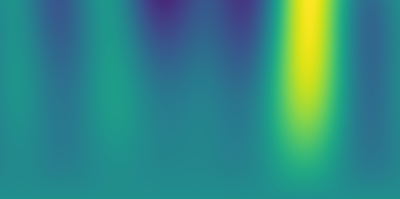
\includegraphics[interpolate=false,width=1.000000in,height=1.000000in]{burgers_exact_pred_0.0-img0.png}}%
\end{pgfscope}%
\begin{pgfscope}%
\pgfsetbuttcap%
\pgfsetroundjoin%
\definecolor{currentfill}{rgb}{0.000000,0.000000,0.000000}%
\pgfsetfillcolor{currentfill}%
\pgfsetlinewidth{0.803000pt}%
\definecolor{currentstroke}{rgb}{0.000000,0.000000,0.000000}%
\pgfsetstrokecolor{currentstroke}%
\pgfsetdash{}{0pt}%
\pgfsys@defobject{currentmarker}{\pgfqpoint{0.000000in}{-0.048611in}}{\pgfqpoint{0.000000in}{0.000000in}}{%
\pgfpathmoveto{\pgfqpoint{0.000000in}{0.000000in}}%
\pgfpathlineto{\pgfqpoint{0.000000in}{-0.048611in}}%
\pgfusepath{stroke,fill}%
}%
\begin{pgfscope}%
\pgfsys@transformshift{0.726837in}{0.517039in}%
\pgfsys@useobject{currentmarker}{}%
\end{pgfscope}%
\end{pgfscope}%
\begin{pgfscope}%
\definecolor{textcolor}{rgb}{0.000000,0.000000,0.000000}%
\pgfsetstrokecolor{textcolor}%
\pgfsetfillcolor{textcolor}%
\pgftext[x=0.726837in,y=0.419816in,,top]{\color{textcolor}{\rmfamily\fontsize{12.000000}{14.400000}\selectfont\catcode`\^=\active\def^{\ifmmode\sp\else\^{}\fi}\catcode`\%=\active\def%{\%}0}}%
\end{pgfscope}%
\begin{pgfscope}%
\pgfsetbuttcap%
\pgfsetroundjoin%
\definecolor{currentfill}{rgb}{0.000000,0.000000,0.000000}%
\pgfsetfillcolor{currentfill}%
\pgfsetlinewidth{0.803000pt}%
\definecolor{currentstroke}{rgb}{0.000000,0.000000,0.000000}%
\pgfsetstrokecolor{currentstroke}%
\pgfsetdash{}{0pt}%
\pgfsys@defobject{currentmarker}{\pgfqpoint{0.000000in}{-0.048611in}}{\pgfqpoint{0.000000in}{0.000000in}}{%
\pgfpathmoveto{\pgfqpoint{0.000000in}{0.000000in}}%
\pgfpathlineto{\pgfqpoint{0.000000in}{-0.048611in}}%
\pgfusepath{stroke,fill}%
}%
\begin{pgfscope}%
\pgfsys@transformshift{1.495229in}{0.517039in}%
\pgfsys@useobject{currentmarker}{}%
\end{pgfscope}%
\end{pgfscope}%
\begin{pgfscope}%
\definecolor{textcolor}{rgb}{0.000000,0.000000,0.000000}%
\pgfsetstrokecolor{textcolor}%
\pgfsetfillcolor{textcolor}%
\pgftext[x=1.495229in,y=0.419816in,,top]{\color{textcolor}{\rmfamily\fontsize{12.000000}{14.400000}\selectfont\catcode`\^=\active\def^{\ifmmode\sp\else\^{}\fi}\catcode`\%=\active\def%{\%}1}}%
\end{pgfscope}%
\begin{pgfscope}%
\pgfsetbuttcap%
\pgfsetroundjoin%
\definecolor{currentfill}{rgb}{0.000000,0.000000,0.000000}%
\pgfsetfillcolor{currentfill}%
\pgfsetlinewidth{0.803000pt}%
\definecolor{currentstroke}{rgb}{0.000000,0.000000,0.000000}%
\pgfsetstrokecolor{currentstroke}%
\pgfsetdash{}{0pt}%
\pgfsys@defobject{currentmarker}{\pgfqpoint{0.000000in}{-0.048611in}}{\pgfqpoint{0.000000in}{0.000000in}}{%
\pgfpathmoveto{\pgfqpoint{0.000000in}{0.000000in}}%
\pgfpathlineto{\pgfqpoint{0.000000in}{-0.048611in}}%
\pgfusepath{stroke,fill}%
}%
\begin{pgfscope}%
\pgfsys@transformshift{2.263621in}{0.517039in}%
\pgfsys@useobject{currentmarker}{}%
\end{pgfscope}%
\end{pgfscope}%
\begin{pgfscope}%
\definecolor{textcolor}{rgb}{0.000000,0.000000,0.000000}%
\pgfsetstrokecolor{textcolor}%
\pgfsetfillcolor{textcolor}%
\pgftext[x=2.263621in,y=0.419816in,,top]{\color{textcolor}{\rmfamily\fontsize{12.000000}{14.400000}\selectfont\catcode`\^=\active\def^{\ifmmode\sp\else\^{}\fi}\catcode`\%=\active\def%{\%}2}}%
\end{pgfscope}%
\begin{pgfscope}%
\definecolor{textcolor}{rgb}{0.000000,0.000000,0.000000}%
\pgfsetstrokecolor{textcolor}%
\pgfsetfillcolor{textcolor}%
\pgftext[x=1.495229in,y=0.202965in,,top]{\color{textcolor}{\rmfamily\fontsize{12.000000}{14.400000}\selectfont\catcode`\^=\active\def^{\ifmmode\sp\else\^{}\fi}\catcode`\%=\active\def%{\%}Space}}%
\end{pgfscope}%
\begin{pgfscope}%
\pgfsetbuttcap%
\pgfsetroundjoin%
\definecolor{currentfill}{rgb}{0.000000,0.000000,0.000000}%
\pgfsetfillcolor{currentfill}%
\pgfsetlinewidth{0.803000pt}%
\definecolor{currentstroke}{rgb}{0.000000,0.000000,0.000000}%
\pgfsetstrokecolor{currentstroke}%
\pgfsetdash{}{0pt}%
\pgfsys@defobject{currentmarker}{\pgfqpoint{-0.048611in}{0.000000in}}{\pgfqpoint{-0.000000in}{0.000000in}}{%
\pgfpathmoveto{\pgfqpoint{-0.000000in}{0.000000in}}%
\pgfpathlineto{\pgfqpoint{-0.048611in}{0.000000in}}%
\pgfusepath{stroke,fill}%
}%
\begin{pgfscope}%
\pgfsys@transformshift{0.726837in}{0.517039in}%
\pgfsys@useobject{currentmarker}{}%
\end{pgfscope}%
\end{pgfscope}%
\begin{pgfscope}%
\definecolor{textcolor}{rgb}{0.000000,0.000000,0.000000}%
\pgfsetstrokecolor{textcolor}%
\pgfsetfillcolor{textcolor}%
\pgftext[x=0.364559in, y=0.453725in, left, base]{\color{textcolor}{\rmfamily\fontsize{12.000000}{14.400000}\selectfont\catcode`\^=\active\def^{\ifmmode\sp\else\^{}\fi}\catcode`\%=\active\def%{\%}0.0}}%
\end{pgfscope}%
\begin{pgfscope}%
\pgfsetbuttcap%
\pgfsetroundjoin%
\definecolor{currentfill}{rgb}{0.000000,0.000000,0.000000}%
\pgfsetfillcolor{currentfill}%
\pgfsetlinewidth{0.803000pt}%
\definecolor{currentstroke}{rgb}{0.000000,0.000000,0.000000}%
\pgfsetstrokecolor{currentstroke}%
\pgfsetdash{}{0pt}%
\pgfsys@defobject{currentmarker}{\pgfqpoint{-0.048611in}{0.000000in}}{\pgfqpoint{-0.000000in}{0.000000in}}{%
\pgfpathmoveto{\pgfqpoint{-0.000000in}{0.000000in}}%
\pgfpathlineto{\pgfqpoint{-0.048611in}{0.000000in}}%
\pgfusepath{stroke,fill}%
}%
\begin{pgfscope}%
\pgfsys@transformshift{0.726837in}{0.861533in}%
\pgfsys@useobject{currentmarker}{}%
\end{pgfscope}%
\end{pgfscope}%
\begin{pgfscope}%
\definecolor{textcolor}{rgb}{0.000000,0.000000,0.000000}%
\pgfsetstrokecolor{textcolor}%
\pgfsetfillcolor{textcolor}%
\pgftext[x=0.364559in, y=0.798219in, left, base]{\color{textcolor}{\rmfamily\fontsize{12.000000}{14.400000}\selectfont\catcode`\^=\active\def^{\ifmmode\sp\else\^{}\fi}\catcode`\%=\active\def%{\%}2.5}}%
\end{pgfscope}%
\begin{pgfscope}%
\pgfsetbuttcap%
\pgfsetroundjoin%
\definecolor{currentfill}{rgb}{0.000000,0.000000,0.000000}%
\pgfsetfillcolor{currentfill}%
\pgfsetlinewidth{0.803000pt}%
\definecolor{currentstroke}{rgb}{0.000000,0.000000,0.000000}%
\pgfsetstrokecolor{currentstroke}%
\pgfsetdash{}{0pt}%
\pgfsys@defobject{currentmarker}{\pgfqpoint{-0.048611in}{0.000000in}}{\pgfqpoint{-0.000000in}{0.000000in}}{%
\pgfpathmoveto{\pgfqpoint{-0.000000in}{0.000000in}}%
\pgfpathlineto{\pgfqpoint{-0.048611in}{0.000000in}}%
\pgfusepath{stroke,fill}%
}%
\begin{pgfscope}%
\pgfsys@transformshift{0.726837in}{1.206027in}%
\pgfsys@useobject{currentmarker}{}%
\end{pgfscope}%
\end{pgfscope}%
\begin{pgfscope}%
\definecolor{textcolor}{rgb}{0.000000,0.000000,0.000000}%
\pgfsetstrokecolor{textcolor}%
\pgfsetfillcolor{textcolor}%
\pgftext[x=0.364559in, y=1.142714in, left, base]{\color{textcolor}{\rmfamily\fontsize{12.000000}{14.400000}\selectfont\catcode`\^=\active\def^{\ifmmode\sp\else\^{}\fi}\catcode`\%=\active\def%{\%}5.0}}%
\end{pgfscope}%
\begin{pgfscope}%
\pgfsetbuttcap%
\pgfsetroundjoin%
\definecolor{currentfill}{rgb}{0.000000,0.000000,0.000000}%
\pgfsetfillcolor{currentfill}%
\pgfsetlinewidth{0.803000pt}%
\definecolor{currentstroke}{rgb}{0.000000,0.000000,0.000000}%
\pgfsetstrokecolor{currentstroke}%
\pgfsetdash{}{0pt}%
\pgfsys@defobject{currentmarker}{\pgfqpoint{-0.048611in}{0.000000in}}{\pgfqpoint{-0.000000in}{0.000000in}}{%
\pgfpathmoveto{\pgfqpoint{-0.000000in}{0.000000in}}%
\pgfpathlineto{\pgfqpoint{-0.048611in}{0.000000in}}%
\pgfusepath{stroke,fill}%
}%
\begin{pgfscope}%
\pgfsys@transformshift{0.726837in}{1.550522in}%
\pgfsys@useobject{currentmarker}{}%
\end{pgfscope}%
\end{pgfscope}%
\begin{pgfscope}%
\definecolor{textcolor}{rgb}{0.000000,0.000000,0.000000}%
\pgfsetstrokecolor{textcolor}%
\pgfsetfillcolor{textcolor}%
\pgftext[x=0.364559in, y=1.487208in, left, base]{\color{textcolor}{\rmfamily\fontsize{12.000000}{14.400000}\selectfont\catcode`\^=\active\def^{\ifmmode\sp\else\^{}\fi}\catcode`\%=\active\def%{\%}7.5}}%
\end{pgfscope}%
\begin{pgfscope}%
\pgfsetbuttcap%
\pgfsetroundjoin%
\definecolor{currentfill}{rgb}{0.000000,0.000000,0.000000}%
\pgfsetfillcolor{currentfill}%
\pgfsetlinewidth{0.803000pt}%
\definecolor{currentstroke}{rgb}{0.000000,0.000000,0.000000}%
\pgfsetstrokecolor{currentstroke}%
\pgfsetdash{}{0pt}%
\pgfsys@defobject{currentmarker}{\pgfqpoint{-0.048611in}{0.000000in}}{\pgfqpoint{-0.000000in}{0.000000in}}{%
\pgfpathmoveto{\pgfqpoint{-0.000000in}{0.000000in}}%
\pgfpathlineto{\pgfqpoint{-0.048611in}{0.000000in}}%
\pgfusepath{stroke,fill}%
}%
\begin{pgfscope}%
\pgfsys@transformshift{0.726837in}{1.895016in}%
\pgfsys@useobject{currentmarker}{}%
\end{pgfscope}%
\end{pgfscope}%
\begin{pgfscope}%
\definecolor{textcolor}{rgb}{0.000000,0.000000,0.000000}%
\pgfsetstrokecolor{textcolor}%
\pgfsetfillcolor{textcolor}%
\pgftext[x=0.258521in, y=1.831702in, left, base]{\color{textcolor}{\rmfamily\fontsize{12.000000}{14.400000}\selectfont\catcode`\^=\active\def^{\ifmmode\sp\else\^{}\fi}\catcode`\%=\active\def%{\%}10.0}}%
\end{pgfscope}%
\begin{pgfscope}%
\definecolor{textcolor}{rgb}{0.000000,0.000000,0.000000}%
\pgfsetstrokecolor{textcolor}%
\pgfsetfillcolor{textcolor}%
\pgftext[x=0.202965in,y=1.206027in,,bottom,rotate=90.000000]{\color{textcolor}{\rmfamily\fontsize{12.000000}{14.400000}\selectfont\catcode`\^=\active\def^{\ifmmode\sp\else\^{}\fi}\catcode`\%=\active\def%{\%}Time}}%
\end{pgfscope}%
\begin{pgfscope}%
\pgfsetrectcap%
\pgfsetmiterjoin%
\pgfsetlinewidth{0.803000pt}%
\definecolor{currentstroke}{rgb}{0.000000,0.000000,0.000000}%
\pgfsetstrokecolor{currentstroke}%
\pgfsetdash{}{0pt}%
\pgfpathmoveto{\pgfqpoint{0.726837in}{0.517039in}}%
\pgfpathlineto{\pgfqpoint{0.726837in}{1.895016in}}%
\pgfusepath{stroke}%
\end{pgfscope}%
\begin{pgfscope}%
\pgfsetrectcap%
\pgfsetmiterjoin%
\pgfsetlinewidth{0.803000pt}%
\definecolor{currentstroke}{rgb}{0.000000,0.000000,0.000000}%
\pgfsetstrokecolor{currentstroke}%
\pgfsetdash{}{0pt}%
\pgfpathmoveto{\pgfqpoint{2.263621in}{0.517039in}}%
\pgfpathlineto{\pgfqpoint{2.263621in}{1.895016in}}%
\pgfusepath{stroke}%
\end{pgfscope}%
\begin{pgfscope}%
\pgfsetrectcap%
\pgfsetmiterjoin%
\pgfsetlinewidth{0.803000pt}%
\definecolor{currentstroke}{rgb}{0.000000,0.000000,0.000000}%
\pgfsetstrokecolor{currentstroke}%
\pgfsetdash{}{0pt}%
\pgfpathmoveto{\pgfqpoint{0.726837in}{0.517039in}}%
\pgfpathlineto{\pgfqpoint{2.263621in}{0.517039in}}%
\pgfusepath{stroke}%
\end{pgfscope}%
\begin{pgfscope}%
\pgfsetrectcap%
\pgfsetmiterjoin%
\pgfsetlinewidth{0.803000pt}%
\definecolor{currentstroke}{rgb}{0.000000,0.000000,0.000000}%
\pgfsetstrokecolor{currentstroke}%
\pgfsetdash{}{0pt}%
\pgfpathmoveto{\pgfqpoint{0.726837in}{1.895016in}}%
\pgfpathlineto{\pgfqpoint{2.263621in}{1.895016in}}%
\pgfusepath{stroke}%
\end{pgfscope}%
\begin{pgfscope}%
\pgfsetbuttcap%
\pgfsetmiterjoin%
\pgfsetlinewidth{0.000000pt}%
\definecolor{currentstroke}{rgb}{0.000000,0.000000,0.000000}%
\pgfsetstrokecolor{currentstroke}%
\pgfsetstrokeopacity{0.000000}%
\pgfsetdash{}{0pt}%
\pgfpathmoveto{\pgfqpoint{2.393479in}{0.517039in}}%
\pgfpathlineto{\pgfqpoint{2.462378in}{0.517039in}}%
\pgfpathlineto{\pgfqpoint{2.462378in}{1.895016in}}%
\pgfpathlineto{\pgfqpoint{2.393479in}{1.895016in}}%
\pgfpathlineto{\pgfqpoint{2.393479in}{0.517039in}}%
\pgfpathclose%
\pgfusepath{}%
\end{pgfscope}%
\begin{pgfscope}%
\pgfsys@transformshift{2.390000in}{0.520000in}%
\pgftext[left,bottom]{
\includegraphics[interpolate=true,width=0.070000in,height=1.380000in]{burgers_exact_pred_0.0-img1.png}}%
\end{pgfscope}%
\begin{pgfscope}%
\pgfsetbuttcap%
\pgfsetroundjoin%
\definecolor{currentfill}{rgb}{0.000000,0.000000,0.000000}%
\pgfsetfillcolor{currentfill}%
\pgfsetlinewidth{0.803000pt}%
\definecolor{currentstroke}{rgb}{0.000000,0.000000,0.000000}%
\pgfsetstrokecolor{currentstroke}%
\pgfsetdash{}{0pt}%
\pgfsys@defobject{currentmarker}{\pgfqpoint{0.000000in}{0.000000in}}{\pgfqpoint{0.048611in}{0.000000in}}{%
\pgfpathmoveto{\pgfqpoint{0.000000in}{0.000000in}}%
\pgfpathlineto{\pgfqpoint{0.048611in}{0.000000in}}%
\pgfusepath{stroke,fill}%
}%
\begin{pgfscope}%
\pgfsys@transformshift{2.462378in}{0.566624in}%
\pgfsys@useobject{currentmarker}{}%
\end{pgfscope}%
\end{pgfscope}%
\begin{pgfscope}%
\definecolor{textcolor}{rgb}{0.000000,0.000000,0.000000}%
\pgfsetstrokecolor{textcolor}%
\pgfsetfillcolor{textcolor}%
\pgftext[x=2.559601in, y=0.503310in, left, base]{\color{textcolor}{\rmfamily\fontsize{12.000000}{14.400000}\selectfont\catcode`\^=\active\def^{\ifmmode\sp\else\^{}\fi}\catcode`\%=\active\def%{\%}\ensuremath{-}0.2}}%
\end{pgfscope}%
\begin{pgfscope}%
\pgfsetbuttcap%
\pgfsetroundjoin%
\definecolor{currentfill}{rgb}{0.000000,0.000000,0.000000}%
\pgfsetfillcolor{currentfill}%
\pgfsetlinewidth{0.803000pt}%
\definecolor{currentstroke}{rgb}{0.000000,0.000000,0.000000}%
\pgfsetstrokecolor{currentstroke}%
\pgfsetdash{}{0pt}%
\pgfsys@defobject{currentmarker}{\pgfqpoint{0.000000in}{0.000000in}}{\pgfqpoint{0.048611in}{0.000000in}}{%
\pgfpathmoveto{\pgfqpoint{0.000000in}{0.000000in}}%
\pgfpathlineto{\pgfqpoint{0.048611in}{0.000000in}}%
\pgfusepath{stroke,fill}%
}%
\begin{pgfscope}%
\pgfsys@transformshift{2.462378in}{1.206027in}%
\pgfsys@useobject{currentmarker}{}%
\end{pgfscope}%
\end{pgfscope}%
\begin{pgfscope}%
\definecolor{textcolor}{rgb}{0.000000,0.000000,0.000000}%
\pgfsetstrokecolor{textcolor}%
\pgfsetfillcolor{textcolor}%
\pgftext[x=2.559601in, y=1.142714in, left, base]{\color{textcolor}{\rmfamily\fontsize{12.000000}{14.400000}\selectfont\catcode`\^=\active\def^{\ifmmode\sp\else\^{}\fi}\catcode`\%=\active\def%{\%}0.0}}%
\end{pgfscope}%
\begin{pgfscope}%
\pgfsetbuttcap%
\pgfsetroundjoin%
\definecolor{currentfill}{rgb}{0.000000,0.000000,0.000000}%
\pgfsetfillcolor{currentfill}%
\pgfsetlinewidth{0.803000pt}%
\definecolor{currentstroke}{rgb}{0.000000,0.000000,0.000000}%
\pgfsetstrokecolor{currentstroke}%
\pgfsetdash{}{0pt}%
\pgfsys@defobject{currentmarker}{\pgfqpoint{0.000000in}{0.000000in}}{\pgfqpoint{0.048611in}{0.000000in}}{%
\pgfpathmoveto{\pgfqpoint{0.000000in}{0.000000in}}%
\pgfpathlineto{\pgfqpoint{0.048611in}{0.000000in}}%
\pgfusepath{stroke,fill}%
}%
\begin{pgfscope}%
\pgfsys@transformshift{2.462378in}{1.845431in}%
\pgfsys@useobject{currentmarker}{}%
\end{pgfscope}%
\end{pgfscope}%
\begin{pgfscope}%
\definecolor{textcolor}{rgb}{0.000000,0.000000,0.000000}%
\pgfsetstrokecolor{textcolor}%
\pgfsetfillcolor{textcolor}%
\pgftext[x=2.559601in, y=1.782117in, left, base]{\color{textcolor}{\rmfamily\fontsize{12.000000}{14.400000}\selectfont\catcode`\^=\active\def^{\ifmmode\sp\else\^{}\fi}\catcode`\%=\active\def%{\%}0.2}}%
\end{pgfscope}%
\begin{pgfscope}%
\pgfsetrectcap%
\pgfsetmiterjoin%
\pgfsetlinewidth{0.803000pt}%
\definecolor{currentstroke}{rgb}{0.000000,0.000000,0.000000}%
\pgfsetstrokecolor{currentstroke}%
\pgfsetdash{}{0pt}%
\pgfpathmoveto{\pgfqpoint{2.393479in}{0.517039in}}%
\pgfpathlineto{\pgfqpoint{2.427929in}{0.517039in}}%
\pgfpathlineto{\pgfqpoint{2.462378in}{0.517039in}}%
\pgfpathlineto{\pgfqpoint{2.462378in}{1.895016in}}%
\pgfpathlineto{\pgfqpoint{2.427929in}{1.895016in}}%
\pgfpathlineto{\pgfqpoint{2.393479in}{1.895016in}}%
\pgfpathlineto{\pgfqpoint{2.393479in}{0.517039in}}%
\pgfpathclose%
\pgfusepath{stroke}%
\end{pgfscope}%
\end{pgfpicture}%
\makeatother%
\endgroup%

      \end{adjustbox}
      \caption{The prediction for \(\nu=0.0\)}\label{fig:sc2_exact_pred_0.0}
    \end{subfigure}
    \begin{subfigure}{0.32\linewidth}
      \begin{adjustbox}{width=\linewidth}
        \begingroup%
\makeatletter%
\begin{pgfpicture}%
\pgfpathrectangle{\pgfpointorigin}{\pgfqpoint{3.000000in}{2.000000in}}%
\pgfusepath{use as bounding box, clip}%
\begin{pgfscope}%
\pgfsetbuttcap%
\pgfsetmiterjoin%
\pgfsetlinewidth{0.000000pt}%
\definecolor{currentstroke}{rgb}{0.000000,0.000000,0.000000}%
\pgfsetstrokecolor{currentstroke}%
\pgfsetstrokeopacity{0.000000}%
\pgfsetdash{}{0pt}%
\pgfpathmoveto{\pgfqpoint{0.000000in}{0.000000in}}%
\pgfpathlineto{\pgfqpoint{3.000000in}{0.000000in}}%
\pgfpathlineto{\pgfqpoint{3.000000in}{2.000000in}}%
\pgfpathlineto{\pgfqpoint{0.000000in}{2.000000in}}%
\pgfpathlineto{\pgfqpoint{0.000000in}{0.000000in}}%
\pgfpathclose%
\pgfusepath{}%
\end{pgfscope}%
\begin{pgfscope}%
\pgfsetbuttcap%
\pgfsetmiterjoin%
\pgfsetlinewidth{0.000000pt}%
\definecolor{currentstroke}{rgb}{0.000000,0.000000,0.000000}%
\pgfsetstrokecolor{currentstroke}%
\pgfsetstrokeopacity{0.000000}%
\pgfsetdash{}{0pt}%
\pgfpathmoveto{\pgfqpoint{0.726837in}{0.517039in}}%
\pgfpathlineto{\pgfqpoint{2.263621in}{0.517039in}}%
\pgfpathlineto{\pgfqpoint{2.263621in}{1.895016in}}%
\pgfpathlineto{\pgfqpoint{0.726837in}{1.895016in}}%
\pgfpathlineto{\pgfqpoint{0.726837in}{0.517039in}}%
\pgfpathclose%
\pgfusepath{}%
\end{pgfscope}%
\begin{pgfscope}%
\pgfpathrectangle{\pgfqpoint{0.726837in}{0.517039in}}{\pgfqpoint{1.536784in}{1.377978in}}%
\pgfusepath{clip}%
\pgfsys@transformcm{1.536784}{0.000000}{0.000000}{1.377978}{0.726837in}{0.517039in}%
\pgftext[left,bottom]{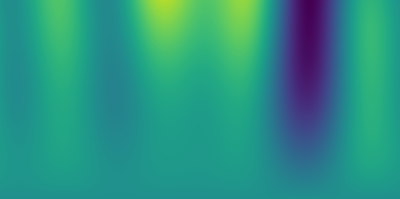
\includegraphics[interpolate=false,width=1.000000in,height=1.000000in]{burgers_exact_diff_0.0-img0.png}}%
\end{pgfscope}%
\begin{pgfscope}%
\pgfsetbuttcap%
\pgfsetroundjoin%
\definecolor{currentfill}{rgb}{0.000000,0.000000,0.000000}%
\pgfsetfillcolor{currentfill}%
\pgfsetlinewidth{0.803000pt}%
\definecolor{currentstroke}{rgb}{0.000000,0.000000,0.000000}%
\pgfsetstrokecolor{currentstroke}%
\pgfsetdash{}{0pt}%
\pgfsys@defobject{currentmarker}{\pgfqpoint{0.000000in}{-0.048611in}}{\pgfqpoint{0.000000in}{0.000000in}}{%
\pgfpathmoveto{\pgfqpoint{0.000000in}{0.000000in}}%
\pgfpathlineto{\pgfqpoint{0.000000in}{-0.048611in}}%
\pgfusepath{stroke,fill}%
}%
\begin{pgfscope}%
\pgfsys@transformshift{0.726837in}{0.517039in}%
\pgfsys@useobject{currentmarker}{}%
\end{pgfscope}%
\end{pgfscope}%
\begin{pgfscope}%
\definecolor{textcolor}{rgb}{0.000000,0.000000,0.000000}%
\pgfsetstrokecolor{textcolor}%
\pgfsetfillcolor{textcolor}%
\pgftext[x=0.726837in,y=0.419816in,,top]{\color{textcolor}\rmfamily\fontsize{12.000000}{14.400000}\selectfont 0}%
\end{pgfscope}%
\begin{pgfscope}%
\pgfsetbuttcap%
\pgfsetroundjoin%
\definecolor{currentfill}{rgb}{0.000000,0.000000,0.000000}%
\pgfsetfillcolor{currentfill}%
\pgfsetlinewidth{0.803000pt}%
\definecolor{currentstroke}{rgb}{0.000000,0.000000,0.000000}%
\pgfsetstrokecolor{currentstroke}%
\pgfsetdash{}{0pt}%
\pgfsys@defobject{currentmarker}{\pgfqpoint{0.000000in}{-0.048611in}}{\pgfqpoint{0.000000in}{0.000000in}}{%
\pgfpathmoveto{\pgfqpoint{0.000000in}{0.000000in}}%
\pgfpathlineto{\pgfqpoint{0.000000in}{-0.048611in}}%
\pgfusepath{stroke,fill}%
}%
\begin{pgfscope}%
\pgfsys@transformshift{1.495229in}{0.517039in}%
\pgfsys@useobject{currentmarker}{}%
\end{pgfscope}%
\end{pgfscope}%
\begin{pgfscope}%
\definecolor{textcolor}{rgb}{0.000000,0.000000,0.000000}%
\pgfsetstrokecolor{textcolor}%
\pgfsetfillcolor{textcolor}%
\pgftext[x=1.495229in,y=0.419816in,,top]{\color{textcolor}\rmfamily\fontsize{12.000000}{14.400000}\selectfont 1}%
\end{pgfscope}%
\begin{pgfscope}%
\pgfsetbuttcap%
\pgfsetroundjoin%
\definecolor{currentfill}{rgb}{0.000000,0.000000,0.000000}%
\pgfsetfillcolor{currentfill}%
\pgfsetlinewidth{0.803000pt}%
\definecolor{currentstroke}{rgb}{0.000000,0.000000,0.000000}%
\pgfsetstrokecolor{currentstroke}%
\pgfsetdash{}{0pt}%
\pgfsys@defobject{currentmarker}{\pgfqpoint{0.000000in}{-0.048611in}}{\pgfqpoint{0.000000in}{0.000000in}}{%
\pgfpathmoveto{\pgfqpoint{0.000000in}{0.000000in}}%
\pgfpathlineto{\pgfqpoint{0.000000in}{-0.048611in}}%
\pgfusepath{stroke,fill}%
}%
\begin{pgfscope}%
\pgfsys@transformshift{2.263621in}{0.517039in}%
\pgfsys@useobject{currentmarker}{}%
\end{pgfscope}%
\end{pgfscope}%
\begin{pgfscope}%
\definecolor{textcolor}{rgb}{0.000000,0.000000,0.000000}%
\pgfsetstrokecolor{textcolor}%
\pgfsetfillcolor{textcolor}%
\pgftext[x=2.263621in,y=0.419816in,,top]{\color{textcolor}\rmfamily\fontsize{12.000000}{14.400000}\selectfont 2}%
\end{pgfscope}%
\begin{pgfscope}%
\definecolor{textcolor}{rgb}{0.000000,0.000000,0.000000}%
\pgfsetstrokecolor{textcolor}%
\pgfsetfillcolor{textcolor}%
\pgftext[x=1.495229in,y=0.202965in,,top]{\color{textcolor}\rmfamily\fontsize{12.000000}{14.400000}\selectfont Space}%
\end{pgfscope}%
\begin{pgfscope}%
\pgfsetbuttcap%
\pgfsetroundjoin%
\definecolor{currentfill}{rgb}{0.000000,0.000000,0.000000}%
\pgfsetfillcolor{currentfill}%
\pgfsetlinewidth{0.803000pt}%
\definecolor{currentstroke}{rgb}{0.000000,0.000000,0.000000}%
\pgfsetstrokecolor{currentstroke}%
\pgfsetdash{}{0pt}%
\pgfsys@defobject{currentmarker}{\pgfqpoint{-0.048611in}{0.000000in}}{\pgfqpoint{-0.000000in}{0.000000in}}{%
\pgfpathmoveto{\pgfqpoint{-0.000000in}{0.000000in}}%
\pgfpathlineto{\pgfqpoint{-0.048611in}{0.000000in}}%
\pgfusepath{stroke,fill}%
}%
\begin{pgfscope}%
\pgfsys@transformshift{0.726837in}{0.517039in}%
\pgfsys@useobject{currentmarker}{}%
\end{pgfscope}%
\end{pgfscope}%
\begin{pgfscope}%
\definecolor{textcolor}{rgb}{0.000000,0.000000,0.000000}%
\pgfsetstrokecolor{textcolor}%
\pgfsetfillcolor{textcolor}%
\pgftext[x=0.364559in, y=0.453725in, left, base]{\color{textcolor}\rmfamily\fontsize{12.000000}{14.400000}\selectfont 0.0}%
\end{pgfscope}%
\begin{pgfscope}%
\pgfsetbuttcap%
\pgfsetroundjoin%
\definecolor{currentfill}{rgb}{0.000000,0.000000,0.000000}%
\pgfsetfillcolor{currentfill}%
\pgfsetlinewidth{0.803000pt}%
\definecolor{currentstroke}{rgb}{0.000000,0.000000,0.000000}%
\pgfsetstrokecolor{currentstroke}%
\pgfsetdash{}{0pt}%
\pgfsys@defobject{currentmarker}{\pgfqpoint{-0.048611in}{0.000000in}}{\pgfqpoint{-0.000000in}{0.000000in}}{%
\pgfpathmoveto{\pgfqpoint{-0.000000in}{0.000000in}}%
\pgfpathlineto{\pgfqpoint{-0.048611in}{0.000000in}}%
\pgfusepath{stroke,fill}%
}%
\begin{pgfscope}%
\pgfsys@transformshift{0.726837in}{0.861533in}%
\pgfsys@useobject{currentmarker}{}%
\end{pgfscope}%
\end{pgfscope}%
\begin{pgfscope}%
\definecolor{textcolor}{rgb}{0.000000,0.000000,0.000000}%
\pgfsetstrokecolor{textcolor}%
\pgfsetfillcolor{textcolor}%
\pgftext[x=0.364559in, y=0.798219in, left, base]{\color{textcolor}\rmfamily\fontsize{12.000000}{14.400000}\selectfont 2.5}%
\end{pgfscope}%
\begin{pgfscope}%
\pgfsetbuttcap%
\pgfsetroundjoin%
\definecolor{currentfill}{rgb}{0.000000,0.000000,0.000000}%
\pgfsetfillcolor{currentfill}%
\pgfsetlinewidth{0.803000pt}%
\definecolor{currentstroke}{rgb}{0.000000,0.000000,0.000000}%
\pgfsetstrokecolor{currentstroke}%
\pgfsetdash{}{0pt}%
\pgfsys@defobject{currentmarker}{\pgfqpoint{-0.048611in}{0.000000in}}{\pgfqpoint{-0.000000in}{0.000000in}}{%
\pgfpathmoveto{\pgfqpoint{-0.000000in}{0.000000in}}%
\pgfpathlineto{\pgfqpoint{-0.048611in}{0.000000in}}%
\pgfusepath{stroke,fill}%
}%
\begin{pgfscope}%
\pgfsys@transformshift{0.726837in}{1.206027in}%
\pgfsys@useobject{currentmarker}{}%
\end{pgfscope}%
\end{pgfscope}%
\begin{pgfscope}%
\definecolor{textcolor}{rgb}{0.000000,0.000000,0.000000}%
\pgfsetstrokecolor{textcolor}%
\pgfsetfillcolor{textcolor}%
\pgftext[x=0.364559in, y=1.142714in, left, base]{\color{textcolor}\rmfamily\fontsize{12.000000}{14.400000}\selectfont 5.0}%
\end{pgfscope}%
\begin{pgfscope}%
\pgfsetbuttcap%
\pgfsetroundjoin%
\definecolor{currentfill}{rgb}{0.000000,0.000000,0.000000}%
\pgfsetfillcolor{currentfill}%
\pgfsetlinewidth{0.803000pt}%
\definecolor{currentstroke}{rgb}{0.000000,0.000000,0.000000}%
\pgfsetstrokecolor{currentstroke}%
\pgfsetdash{}{0pt}%
\pgfsys@defobject{currentmarker}{\pgfqpoint{-0.048611in}{0.000000in}}{\pgfqpoint{-0.000000in}{0.000000in}}{%
\pgfpathmoveto{\pgfqpoint{-0.000000in}{0.000000in}}%
\pgfpathlineto{\pgfqpoint{-0.048611in}{0.000000in}}%
\pgfusepath{stroke,fill}%
}%
\begin{pgfscope}%
\pgfsys@transformshift{0.726837in}{1.550522in}%
\pgfsys@useobject{currentmarker}{}%
\end{pgfscope}%
\end{pgfscope}%
\begin{pgfscope}%
\definecolor{textcolor}{rgb}{0.000000,0.000000,0.000000}%
\pgfsetstrokecolor{textcolor}%
\pgfsetfillcolor{textcolor}%
\pgftext[x=0.364559in, y=1.487208in, left, base]{\color{textcolor}\rmfamily\fontsize{12.000000}{14.400000}\selectfont 7.5}%
\end{pgfscope}%
\begin{pgfscope}%
\pgfsetbuttcap%
\pgfsetroundjoin%
\definecolor{currentfill}{rgb}{0.000000,0.000000,0.000000}%
\pgfsetfillcolor{currentfill}%
\pgfsetlinewidth{0.803000pt}%
\definecolor{currentstroke}{rgb}{0.000000,0.000000,0.000000}%
\pgfsetstrokecolor{currentstroke}%
\pgfsetdash{}{0pt}%
\pgfsys@defobject{currentmarker}{\pgfqpoint{-0.048611in}{0.000000in}}{\pgfqpoint{-0.000000in}{0.000000in}}{%
\pgfpathmoveto{\pgfqpoint{-0.000000in}{0.000000in}}%
\pgfpathlineto{\pgfqpoint{-0.048611in}{0.000000in}}%
\pgfusepath{stroke,fill}%
}%
\begin{pgfscope}%
\pgfsys@transformshift{0.726837in}{1.895016in}%
\pgfsys@useobject{currentmarker}{}%
\end{pgfscope}%
\end{pgfscope}%
\begin{pgfscope}%
\definecolor{textcolor}{rgb}{0.000000,0.000000,0.000000}%
\pgfsetstrokecolor{textcolor}%
\pgfsetfillcolor{textcolor}%
\pgftext[x=0.258521in, y=1.831702in, left, base]{\color{textcolor}\rmfamily\fontsize{12.000000}{14.400000}\selectfont 10.0}%
\end{pgfscope}%
\begin{pgfscope}%
\definecolor{textcolor}{rgb}{0.000000,0.000000,0.000000}%
\pgfsetstrokecolor{textcolor}%
\pgfsetfillcolor{textcolor}%
\pgftext[x=0.202965in,y=1.206027in,,bottom,rotate=90.000000]{\color{textcolor}\rmfamily\fontsize{12.000000}{14.400000}\selectfont Time}%
\end{pgfscope}%
\begin{pgfscope}%
\pgfsetrectcap%
\pgfsetmiterjoin%
\pgfsetlinewidth{0.803000pt}%
\definecolor{currentstroke}{rgb}{0.000000,0.000000,0.000000}%
\pgfsetstrokecolor{currentstroke}%
\pgfsetdash{}{0pt}%
\pgfpathmoveto{\pgfqpoint{0.726837in}{0.517039in}}%
\pgfpathlineto{\pgfqpoint{0.726837in}{1.895016in}}%
\pgfusepath{stroke}%
\end{pgfscope}%
\begin{pgfscope}%
\pgfsetrectcap%
\pgfsetmiterjoin%
\pgfsetlinewidth{0.803000pt}%
\definecolor{currentstroke}{rgb}{0.000000,0.000000,0.000000}%
\pgfsetstrokecolor{currentstroke}%
\pgfsetdash{}{0pt}%
\pgfpathmoveto{\pgfqpoint{2.263621in}{0.517039in}}%
\pgfpathlineto{\pgfqpoint{2.263621in}{1.895016in}}%
\pgfusepath{stroke}%
\end{pgfscope}%
\begin{pgfscope}%
\pgfsetrectcap%
\pgfsetmiterjoin%
\pgfsetlinewidth{0.803000pt}%
\definecolor{currentstroke}{rgb}{0.000000,0.000000,0.000000}%
\pgfsetstrokecolor{currentstroke}%
\pgfsetdash{}{0pt}%
\pgfpathmoveto{\pgfqpoint{0.726837in}{0.517039in}}%
\pgfpathlineto{\pgfqpoint{2.263621in}{0.517039in}}%
\pgfusepath{stroke}%
\end{pgfscope}%
\begin{pgfscope}%
\pgfsetrectcap%
\pgfsetmiterjoin%
\pgfsetlinewidth{0.803000pt}%
\definecolor{currentstroke}{rgb}{0.000000,0.000000,0.000000}%
\pgfsetstrokecolor{currentstroke}%
\pgfsetdash{}{0pt}%
\pgfpathmoveto{\pgfqpoint{0.726837in}{1.895016in}}%
\pgfpathlineto{\pgfqpoint{2.263621in}{1.895016in}}%
\pgfusepath{stroke}%
\end{pgfscope}%
\begin{pgfscope}%
\pgfsetbuttcap%
\pgfsetmiterjoin%
\pgfsetlinewidth{0.000000pt}%
\definecolor{currentstroke}{rgb}{0.000000,0.000000,0.000000}%
\pgfsetstrokecolor{currentstroke}%
\pgfsetstrokeopacity{0.000000}%
\pgfsetdash{}{0pt}%
\pgfpathmoveto{\pgfqpoint{2.393479in}{0.517039in}}%
\pgfpathlineto{\pgfqpoint{2.462378in}{0.517039in}}%
\pgfpathlineto{\pgfqpoint{2.462378in}{1.895016in}}%
\pgfpathlineto{\pgfqpoint{2.393479in}{1.895016in}}%
\pgfpathlineto{\pgfqpoint{2.393479in}{0.517039in}}%
\pgfpathclose%
\pgfusepath{}%
\end{pgfscope}%
\begin{pgfscope}%
\pgfsys@transformshift{2.390000in}{0.520000in}%
\pgftext[left,bottom]{
\includegraphics[interpolate=true,width=0.070000in,height=1.380000in]{burgers_exact_diff_0.0-img1.png}}%
\end{pgfscope}%
\begin{pgfscope}%
\pgfsetbuttcap%
\pgfsetroundjoin%
\definecolor{currentfill}{rgb}{0.000000,0.000000,0.000000}%
\pgfsetfillcolor{currentfill}%
\pgfsetlinewidth{0.803000pt}%
\definecolor{currentstroke}{rgb}{0.000000,0.000000,0.000000}%
\pgfsetstrokecolor{currentstroke}%
\pgfsetdash{}{0pt}%
\pgfsys@defobject{currentmarker}{\pgfqpoint{0.000000in}{0.000000in}}{\pgfqpoint{0.048611in}{0.000000in}}{%
\pgfpathmoveto{\pgfqpoint{0.000000in}{0.000000in}}%
\pgfpathlineto{\pgfqpoint{0.048611in}{0.000000in}}%
\pgfusepath{stroke,fill}%
}%
\begin{pgfscope}%
\pgfsys@transformshift{2.462378in}{0.565953in}%
\pgfsys@useobject{currentmarker}{}%
\end{pgfscope}%
\end{pgfscope}%
\begin{pgfscope}%
\definecolor{textcolor}{rgb}{0.000000,0.000000,0.000000}%
\pgfsetstrokecolor{textcolor}%
\pgfsetfillcolor{textcolor}%
\pgftext[x=2.559601in, y=0.502639in, left, base]{\color{textcolor}\rmfamily\fontsize{12.000000}{14.400000}\selectfont \ensuremath{-}0.2}%
\end{pgfscope}%
\begin{pgfscope}%
\pgfsetbuttcap%
\pgfsetroundjoin%
\definecolor{currentfill}{rgb}{0.000000,0.000000,0.000000}%
\pgfsetfillcolor{currentfill}%
\pgfsetlinewidth{0.803000pt}%
\definecolor{currentstroke}{rgb}{0.000000,0.000000,0.000000}%
\pgfsetstrokecolor{currentstroke}%
\pgfsetdash{}{0pt}%
\pgfsys@defobject{currentmarker}{\pgfqpoint{0.000000in}{0.000000in}}{\pgfqpoint{0.048611in}{0.000000in}}{%
\pgfpathmoveto{\pgfqpoint{0.000000in}{0.000000in}}%
\pgfpathlineto{\pgfqpoint{0.048611in}{0.000000in}}%
\pgfusepath{stroke,fill}%
}%
\begin{pgfscope}%
\pgfsys@transformshift{2.462378in}{1.206027in}%
\pgfsys@useobject{currentmarker}{}%
\end{pgfscope}%
\end{pgfscope}%
\begin{pgfscope}%
\definecolor{textcolor}{rgb}{0.000000,0.000000,0.000000}%
\pgfsetstrokecolor{textcolor}%
\pgfsetfillcolor{textcolor}%
\pgftext[x=2.559601in, y=1.142714in, left, base]{\color{textcolor}\rmfamily\fontsize{12.000000}{14.400000}\selectfont 0.0}%
\end{pgfscope}%
\begin{pgfscope}%
\pgfsetbuttcap%
\pgfsetroundjoin%
\definecolor{currentfill}{rgb}{0.000000,0.000000,0.000000}%
\pgfsetfillcolor{currentfill}%
\pgfsetlinewidth{0.803000pt}%
\definecolor{currentstroke}{rgb}{0.000000,0.000000,0.000000}%
\pgfsetstrokecolor{currentstroke}%
\pgfsetdash{}{0pt}%
\pgfsys@defobject{currentmarker}{\pgfqpoint{0.000000in}{0.000000in}}{\pgfqpoint{0.048611in}{0.000000in}}{%
\pgfpathmoveto{\pgfqpoint{0.000000in}{0.000000in}}%
\pgfpathlineto{\pgfqpoint{0.048611in}{0.000000in}}%
\pgfusepath{stroke,fill}%
}%
\begin{pgfscope}%
\pgfsys@transformshift{2.462378in}{1.846102in}%
\pgfsys@useobject{currentmarker}{}%
\end{pgfscope}%
\end{pgfscope}%
\begin{pgfscope}%
\definecolor{textcolor}{rgb}{0.000000,0.000000,0.000000}%
\pgfsetstrokecolor{textcolor}%
\pgfsetfillcolor{textcolor}%
\pgftext[x=2.559601in, y=1.782788in, left, base]{\color{textcolor}\rmfamily\fontsize{12.000000}{14.400000}\selectfont 0.2}%
\end{pgfscope}%
\begin{pgfscope}%
\pgfsetrectcap%
\pgfsetmiterjoin%
\pgfsetlinewidth{0.803000pt}%
\definecolor{currentstroke}{rgb}{0.000000,0.000000,0.000000}%
\pgfsetstrokecolor{currentstroke}%
\pgfsetdash{}{0pt}%
\pgfpathmoveto{\pgfqpoint{2.393479in}{0.517039in}}%
\pgfpathlineto{\pgfqpoint{2.427929in}{0.517039in}}%
\pgfpathlineto{\pgfqpoint{2.462378in}{0.517039in}}%
\pgfpathlineto{\pgfqpoint{2.462378in}{1.895016in}}%
\pgfpathlineto{\pgfqpoint{2.427929in}{1.895016in}}%
\pgfpathlineto{\pgfqpoint{2.393479in}{1.895016in}}%
\pgfpathlineto{\pgfqpoint{2.393479in}{0.517039in}}%
\pgfpathclose%
\pgfusepath{stroke}%
\end{pgfscope}%
\end{pgfpicture}%
\makeatother%
\endgroup%

      \end{adjustbox}
      \caption{The difference for \(\nu=0.0\)}\label{fig:sc2_exact_diff_0.0}
    \end{subfigure}
    \\[0.7\baselineskip]
    \begin{subfigure}{0.33\linewidth}
      \begin{adjustbox}{width=\linewidth}
        \begingroup%
\makeatletter%
\begin{pgfpicture}%
\pgfpathrectangle{\pgfpointorigin}{\pgfqpoint{3.000000in}{2.000000in}}%
\pgfusepath{use as bounding box, clip}%
\begin{pgfscope}%
\pgfsetbuttcap%
\pgfsetmiterjoin%
\pgfsetlinewidth{0.000000pt}%
\definecolor{currentstroke}{rgb}{0.000000,0.000000,0.000000}%
\pgfsetstrokecolor{currentstroke}%
\pgfsetstrokeopacity{0.000000}%
\pgfsetdash{}{0pt}%
\pgfpathmoveto{\pgfqpoint{0.000000in}{0.000000in}}%
\pgfpathlineto{\pgfqpoint{3.000000in}{0.000000in}}%
\pgfpathlineto{\pgfqpoint{3.000000in}{2.000000in}}%
\pgfpathlineto{\pgfqpoint{0.000000in}{2.000000in}}%
\pgfpathlineto{\pgfqpoint{0.000000in}{0.000000in}}%
\pgfpathclose%
\pgfusepath{}%
\end{pgfscope}%
\begin{pgfscope}%
\pgfsetbuttcap%
\pgfsetmiterjoin%
\pgfsetlinewidth{0.000000pt}%
\definecolor{currentstroke}{rgb}{0.000000,0.000000,0.000000}%
\pgfsetstrokecolor{currentstroke}%
\pgfsetstrokeopacity{0.000000}%
\pgfsetdash{}{0pt}%
\pgfpathmoveto{\pgfqpoint{0.726837in}{0.517039in}}%
\pgfpathlineto{\pgfqpoint{2.263621in}{0.517039in}}%
\pgfpathlineto{\pgfqpoint{2.263621in}{1.895016in}}%
\pgfpathlineto{\pgfqpoint{0.726837in}{1.895016in}}%
\pgfpathlineto{\pgfqpoint{0.726837in}{0.517039in}}%
\pgfpathclose%
\pgfusepath{}%
\end{pgfscope}%
\begin{pgfscope}%
\pgfpathrectangle{\pgfqpoint{0.726837in}{0.517039in}}{\pgfqpoint{1.536784in}{1.377978in}}%
\pgfusepath{clip}%
\pgfsys@transformcm{1.536784}{0.000000}{0.000000}{1.377978}{0.726837in}{0.517039in}%
\pgftext[left,bottom]{
\includegraphics[interpolate=false,width=1.000000in,height=1.000000in]{burgers_exact_target_0.01-img0.png}}%
\end{pgfscope}%
\begin{pgfscope}%
\pgfsetbuttcap%
\pgfsetroundjoin%
\definecolor{currentfill}{rgb}{0.000000,0.000000,0.000000}%
\pgfsetfillcolor{currentfill}%
\pgfsetlinewidth{0.803000pt}%
\definecolor{currentstroke}{rgb}{0.000000,0.000000,0.000000}%
\pgfsetstrokecolor{currentstroke}%
\pgfsetdash{}{0pt}%
\pgfsys@defobject{currentmarker}{\pgfqpoint{0.000000in}{-0.048611in}}{\pgfqpoint{0.000000in}{0.000000in}}{%
\pgfpathmoveto{\pgfqpoint{0.000000in}{0.000000in}}%
\pgfpathlineto{\pgfqpoint{0.000000in}{-0.048611in}}%
\pgfusepath{stroke,fill}%
}%
\begin{pgfscope}%
\pgfsys@transformshift{0.726837in}{0.517039in}%
\pgfsys@useobject{currentmarker}{}%
\end{pgfscope}%
\end{pgfscope}%
\begin{pgfscope}%
\definecolor{textcolor}{rgb}{0.000000,0.000000,0.000000}%
\pgfsetstrokecolor{textcolor}%
\pgfsetfillcolor{textcolor}%
\pgftext[x=0.726837in,y=0.419816in,,top]{\color{textcolor}\rmfamily\fontsize{12.000000}{14.400000}\selectfont 0}%
\end{pgfscope}%
\begin{pgfscope}%
\pgfsetbuttcap%
\pgfsetroundjoin%
\definecolor{currentfill}{rgb}{0.000000,0.000000,0.000000}%
\pgfsetfillcolor{currentfill}%
\pgfsetlinewidth{0.803000pt}%
\definecolor{currentstroke}{rgb}{0.000000,0.000000,0.000000}%
\pgfsetstrokecolor{currentstroke}%
\pgfsetdash{}{0pt}%
\pgfsys@defobject{currentmarker}{\pgfqpoint{0.000000in}{-0.048611in}}{\pgfqpoint{0.000000in}{0.000000in}}{%
\pgfpathmoveto{\pgfqpoint{0.000000in}{0.000000in}}%
\pgfpathlineto{\pgfqpoint{0.000000in}{-0.048611in}}%
\pgfusepath{stroke,fill}%
}%
\begin{pgfscope}%
\pgfsys@transformshift{1.495229in}{0.517039in}%
\pgfsys@useobject{currentmarker}{}%
\end{pgfscope}%
\end{pgfscope}%
\begin{pgfscope}%
\definecolor{textcolor}{rgb}{0.000000,0.000000,0.000000}%
\pgfsetstrokecolor{textcolor}%
\pgfsetfillcolor{textcolor}%
\pgftext[x=1.495229in,y=0.419816in,,top]{\color{textcolor}\rmfamily\fontsize{12.000000}{14.400000}\selectfont 1}%
\end{pgfscope}%
\begin{pgfscope}%
\pgfsetbuttcap%
\pgfsetroundjoin%
\definecolor{currentfill}{rgb}{0.000000,0.000000,0.000000}%
\pgfsetfillcolor{currentfill}%
\pgfsetlinewidth{0.803000pt}%
\definecolor{currentstroke}{rgb}{0.000000,0.000000,0.000000}%
\pgfsetstrokecolor{currentstroke}%
\pgfsetdash{}{0pt}%
\pgfsys@defobject{currentmarker}{\pgfqpoint{0.000000in}{-0.048611in}}{\pgfqpoint{0.000000in}{0.000000in}}{%
\pgfpathmoveto{\pgfqpoint{0.000000in}{0.000000in}}%
\pgfpathlineto{\pgfqpoint{0.000000in}{-0.048611in}}%
\pgfusepath{stroke,fill}%
}%
\begin{pgfscope}%
\pgfsys@transformshift{2.263621in}{0.517039in}%
\pgfsys@useobject{currentmarker}{}%
\end{pgfscope}%
\end{pgfscope}%
\begin{pgfscope}%
\definecolor{textcolor}{rgb}{0.000000,0.000000,0.000000}%
\pgfsetstrokecolor{textcolor}%
\pgfsetfillcolor{textcolor}%
\pgftext[x=2.263621in,y=0.419816in,,top]{\color{textcolor}\rmfamily\fontsize{12.000000}{14.400000}\selectfont 2}%
\end{pgfscope}%
\begin{pgfscope}%
\definecolor{textcolor}{rgb}{0.000000,0.000000,0.000000}%
\pgfsetstrokecolor{textcolor}%
\pgfsetfillcolor{textcolor}%
\pgftext[x=1.495229in,y=0.202965in,,top]{\color{textcolor}\rmfamily\fontsize{12.000000}{14.400000}\selectfont Space}%
\end{pgfscope}%
\begin{pgfscope}%
\pgfsetbuttcap%
\pgfsetroundjoin%
\definecolor{currentfill}{rgb}{0.000000,0.000000,0.000000}%
\pgfsetfillcolor{currentfill}%
\pgfsetlinewidth{0.803000pt}%
\definecolor{currentstroke}{rgb}{0.000000,0.000000,0.000000}%
\pgfsetstrokecolor{currentstroke}%
\pgfsetdash{}{0pt}%
\pgfsys@defobject{currentmarker}{\pgfqpoint{-0.048611in}{0.000000in}}{\pgfqpoint{-0.000000in}{0.000000in}}{%
\pgfpathmoveto{\pgfqpoint{-0.000000in}{0.000000in}}%
\pgfpathlineto{\pgfqpoint{-0.048611in}{0.000000in}}%
\pgfusepath{stroke,fill}%
}%
\begin{pgfscope}%
\pgfsys@transformshift{0.726837in}{0.517039in}%
\pgfsys@useobject{currentmarker}{}%
\end{pgfscope}%
\end{pgfscope}%
\begin{pgfscope}%
\definecolor{textcolor}{rgb}{0.000000,0.000000,0.000000}%
\pgfsetstrokecolor{textcolor}%
\pgfsetfillcolor{textcolor}%
\pgftext[x=0.364559in, y=0.453725in, left, base]{\color{textcolor}\rmfamily\fontsize{12.000000}{14.400000}\selectfont 0.0}%
\end{pgfscope}%
\begin{pgfscope}%
\pgfsetbuttcap%
\pgfsetroundjoin%
\definecolor{currentfill}{rgb}{0.000000,0.000000,0.000000}%
\pgfsetfillcolor{currentfill}%
\pgfsetlinewidth{0.803000pt}%
\definecolor{currentstroke}{rgb}{0.000000,0.000000,0.000000}%
\pgfsetstrokecolor{currentstroke}%
\pgfsetdash{}{0pt}%
\pgfsys@defobject{currentmarker}{\pgfqpoint{-0.048611in}{0.000000in}}{\pgfqpoint{-0.000000in}{0.000000in}}{%
\pgfpathmoveto{\pgfqpoint{-0.000000in}{0.000000in}}%
\pgfpathlineto{\pgfqpoint{-0.048611in}{0.000000in}}%
\pgfusepath{stroke,fill}%
}%
\begin{pgfscope}%
\pgfsys@transformshift{0.726837in}{0.861533in}%
\pgfsys@useobject{currentmarker}{}%
\end{pgfscope}%
\end{pgfscope}%
\begin{pgfscope}%
\definecolor{textcolor}{rgb}{0.000000,0.000000,0.000000}%
\pgfsetstrokecolor{textcolor}%
\pgfsetfillcolor{textcolor}%
\pgftext[x=0.364559in, y=0.798219in, left, base]{\color{textcolor}\rmfamily\fontsize{12.000000}{14.400000}\selectfont 2.5}%
\end{pgfscope}%
\begin{pgfscope}%
\pgfsetbuttcap%
\pgfsetroundjoin%
\definecolor{currentfill}{rgb}{0.000000,0.000000,0.000000}%
\pgfsetfillcolor{currentfill}%
\pgfsetlinewidth{0.803000pt}%
\definecolor{currentstroke}{rgb}{0.000000,0.000000,0.000000}%
\pgfsetstrokecolor{currentstroke}%
\pgfsetdash{}{0pt}%
\pgfsys@defobject{currentmarker}{\pgfqpoint{-0.048611in}{0.000000in}}{\pgfqpoint{-0.000000in}{0.000000in}}{%
\pgfpathmoveto{\pgfqpoint{-0.000000in}{0.000000in}}%
\pgfpathlineto{\pgfqpoint{-0.048611in}{0.000000in}}%
\pgfusepath{stroke,fill}%
}%
\begin{pgfscope}%
\pgfsys@transformshift{0.726837in}{1.206027in}%
\pgfsys@useobject{currentmarker}{}%
\end{pgfscope}%
\end{pgfscope}%
\begin{pgfscope}%
\definecolor{textcolor}{rgb}{0.000000,0.000000,0.000000}%
\pgfsetstrokecolor{textcolor}%
\pgfsetfillcolor{textcolor}%
\pgftext[x=0.364559in, y=1.142714in, left, base]{\color{textcolor}\rmfamily\fontsize{12.000000}{14.400000}\selectfont 5.0}%
\end{pgfscope}%
\begin{pgfscope}%
\pgfsetbuttcap%
\pgfsetroundjoin%
\definecolor{currentfill}{rgb}{0.000000,0.000000,0.000000}%
\pgfsetfillcolor{currentfill}%
\pgfsetlinewidth{0.803000pt}%
\definecolor{currentstroke}{rgb}{0.000000,0.000000,0.000000}%
\pgfsetstrokecolor{currentstroke}%
\pgfsetdash{}{0pt}%
\pgfsys@defobject{currentmarker}{\pgfqpoint{-0.048611in}{0.000000in}}{\pgfqpoint{-0.000000in}{0.000000in}}{%
\pgfpathmoveto{\pgfqpoint{-0.000000in}{0.000000in}}%
\pgfpathlineto{\pgfqpoint{-0.048611in}{0.000000in}}%
\pgfusepath{stroke,fill}%
}%
\begin{pgfscope}%
\pgfsys@transformshift{0.726837in}{1.550522in}%
\pgfsys@useobject{currentmarker}{}%
\end{pgfscope}%
\end{pgfscope}%
\begin{pgfscope}%
\definecolor{textcolor}{rgb}{0.000000,0.000000,0.000000}%
\pgfsetstrokecolor{textcolor}%
\pgfsetfillcolor{textcolor}%
\pgftext[x=0.364559in, y=1.487208in, left, base]{\color{textcolor}\rmfamily\fontsize{12.000000}{14.400000}\selectfont 7.5}%
\end{pgfscope}%
\begin{pgfscope}%
\pgfsetbuttcap%
\pgfsetroundjoin%
\definecolor{currentfill}{rgb}{0.000000,0.000000,0.000000}%
\pgfsetfillcolor{currentfill}%
\pgfsetlinewidth{0.803000pt}%
\definecolor{currentstroke}{rgb}{0.000000,0.000000,0.000000}%
\pgfsetstrokecolor{currentstroke}%
\pgfsetdash{}{0pt}%
\pgfsys@defobject{currentmarker}{\pgfqpoint{-0.048611in}{0.000000in}}{\pgfqpoint{-0.000000in}{0.000000in}}{%
\pgfpathmoveto{\pgfqpoint{-0.000000in}{0.000000in}}%
\pgfpathlineto{\pgfqpoint{-0.048611in}{0.000000in}}%
\pgfusepath{stroke,fill}%
}%
\begin{pgfscope}%
\pgfsys@transformshift{0.726837in}{1.895016in}%
\pgfsys@useobject{currentmarker}{}%
\end{pgfscope}%
\end{pgfscope}%
\begin{pgfscope}%
\definecolor{textcolor}{rgb}{0.000000,0.000000,0.000000}%
\pgfsetstrokecolor{textcolor}%
\pgfsetfillcolor{textcolor}%
\pgftext[x=0.258521in, y=1.831702in, left, base]{\color{textcolor}\rmfamily\fontsize{12.000000}{14.400000}\selectfont 10.0}%
\end{pgfscope}%
\begin{pgfscope}%
\definecolor{textcolor}{rgb}{0.000000,0.000000,0.000000}%
\pgfsetstrokecolor{textcolor}%
\pgfsetfillcolor{textcolor}%
\pgftext[x=0.202965in,y=1.206027in,,bottom,rotate=90.000000]{\color{textcolor}\rmfamily\fontsize{12.000000}{14.400000}\selectfont Time}%
\end{pgfscope}%
\begin{pgfscope}%
\pgfsetrectcap%
\pgfsetmiterjoin%
\pgfsetlinewidth{0.803000pt}%
\definecolor{currentstroke}{rgb}{0.000000,0.000000,0.000000}%
\pgfsetstrokecolor{currentstroke}%
\pgfsetdash{}{0pt}%
\pgfpathmoveto{\pgfqpoint{0.726837in}{0.517039in}}%
\pgfpathlineto{\pgfqpoint{0.726837in}{1.895016in}}%
\pgfusepath{stroke}%
\end{pgfscope}%
\begin{pgfscope}%
\pgfsetrectcap%
\pgfsetmiterjoin%
\pgfsetlinewidth{0.803000pt}%
\definecolor{currentstroke}{rgb}{0.000000,0.000000,0.000000}%
\pgfsetstrokecolor{currentstroke}%
\pgfsetdash{}{0pt}%
\pgfpathmoveto{\pgfqpoint{2.263621in}{0.517039in}}%
\pgfpathlineto{\pgfqpoint{2.263621in}{1.895016in}}%
\pgfusepath{stroke}%
\end{pgfscope}%
\begin{pgfscope}%
\pgfsetrectcap%
\pgfsetmiterjoin%
\pgfsetlinewidth{0.803000pt}%
\definecolor{currentstroke}{rgb}{0.000000,0.000000,0.000000}%
\pgfsetstrokecolor{currentstroke}%
\pgfsetdash{}{0pt}%
\pgfpathmoveto{\pgfqpoint{0.726837in}{0.517039in}}%
\pgfpathlineto{\pgfqpoint{2.263621in}{0.517039in}}%
\pgfusepath{stroke}%
\end{pgfscope}%
\begin{pgfscope}%
\pgfsetrectcap%
\pgfsetmiterjoin%
\pgfsetlinewidth{0.803000pt}%
\definecolor{currentstroke}{rgb}{0.000000,0.000000,0.000000}%
\pgfsetstrokecolor{currentstroke}%
\pgfsetdash{}{0pt}%
\pgfpathmoveto{\pgfqpoint{0.726837in}{1.895016in}}%
\pgfpathlineto{\pgfqpoint{2.263621in}{1.895016in}}%
\pgfusepath{stroke}%
\end{pgfscope}%
\begin{pgfscope}%
\pgfsetbuttcap%
\pgfsetmiterjoin%
\pgfsetlinewidth{0.000000pt}%
\definecolor{currentstroke}{rgb}{0.000000,0.000000,0.000000}%
\pgfsetstrokecolor{currentstroke}%
\pgfsetstrokeopacity{0.000000}%
\pgfsetdash{}{0pt}%
\pgfpathmoveto{\pgfqpoint{2.393479in}{0.517039in}}%
\pgfpathlineto{\pgfqpoint{2.462378in}{0.517039in}}%
\pgfpathlineto{\pgfqpoint{2.462378in}{1.895016in}}%
\pgfpathlineto{\pgfqpoint{2.393479in}{1.895016in}}%
\pgfpathlineto{\pgfqpoint{2.393479in}{0.517039in}}%
\pgfpathclose%
\pgfusepath{}%
\end{pgfscope}%
\begin{pgfscope}%
\pgfsys@transformshift{2.390000in}{0.520000in}%
\pgftext[left,bottom]{
\includegraphics[interpolate=true,width=0.070000in,height=1.380000in]{burgers_exact_target_0.01-img1.png}}%
\end{pgfscope}%
\begin{pgfscope}%
\pgfsetbuttcap%
\pgfsetroundjoin%
\definecolor{currentfill}{rgb}{0.000000,0.000000,0.000000}%
\pgfsetfillcolor{currentfill}%
\pgfsetlinewidth{0.803000pt}%
\definecolor{currentstroke}{rgb}{0.000000,0.000000,0.000000}%
\pgfsetstrokecolor{currentstroke}%
\pgfsetdash{}{0pt}%
\pgfsys@defobject{currentmarker}{\pgfqpoint{0.000000in}{0.000000in}}{\pgfqpoint{0.048611in}{0.000000in}}{%
\pgfpathmoveto{\pgfqpoint{0.000000in}{0.000000in}}%
\pgfpathlineto{\pgfqpoint{0.048611in}{0.000000in}}%
\pgfusepath{stroke,fill}%
}%
\begin{pgfscope}%
\pgfsys@transformshift{2.462378in}{0.649681in}%
\pgfsys@useobject{currentmarker}{}%
\end{pgfscope}%
\end{pgfscope}%
\begin{pgfscope}%
\definecolor{textcolor}{rgb}{0.000000,0.000000,0.000000}%
\pgfsetstrokecolor{textcolor}%
\pgfsetfillcolor{textcolor}%
\pgftext[x=2.559601in, y=0.586367in, left, base]{\color{textcolor}\rmfamily\fontsize{12.000000}{14.400000}\selectfont \ensuremath{-}0.1}%
\end{pgfscope}%
\begin{pgfscope}%
\pgfsetbuttcap%
\pgfsetroundjoin%
\definecolor{currentfill}{rgb}{0.000000,0.000000,0.000000}%
\pgfsetfillcolor{currentfill}%
\pgfsetlinewidth{0.803000pt}%
\definecolor{currentstroke}{rgb}{0.000000,0.000000,0.000000}%
\pgfsetstrokecolor{currentstroke}%
\pgfsetdash{}{0pt}%
\pgfsys@defobject{currentmarker}{\pgfqpoint{0.000000in}{0.000000in}}{\pgfqpoint{0.048611in}{0.000000in}}{%
\pgfpathmoveto{\pgfqpoint{0.000000in}{0.000000in}}%
\pgfpathlineto{\pgfqpoint{0.048611in}{0.000000in}}%
\pgfusepath{stroke,fill}%
}%
\begin{pgfscope}%
\pgfsys@transformshift{2.462378in}{1.206027in}%
\pgfsys@useobject{currentmarker}{}%
\end{pgfscope}%
\end{pgfscope}%
\begin{pgfscope}%
\definecolor{textcolor}{rgb}{0.000000,0.000000,0.000000}%
\pgfsetstrokecolor{textcolor}%
\pgfsetfillcolor{textcolor}%
\pgftext[x=2.559601in, y=1.142714in, left, base]{\color{textcolor}\rmfamily\fontsize{12.000000}{14.400000}\selectfont 0.0}%
\end{pgfscope}%
\begin{pgfscope}%
\pgfsetbuttcap%
\pgfsetroundjoin%
\definecolor{currentfill}{rgb}{0.000000,0.000000,0.000000}%
\pgfsetfillcolor{currentfill}%
\pgfsetlinewidth{0.803000pt}%
\definecolor{currentstroke}{rgb}{0.000000,0.000000,0.000000}%
\pgfsetstrokecolor{currentstroke}%
\pgfsetdash{}{0pt}%
\pgfsys@defobject{currentmarker}{\pgfqpoint{0.000000in}{0.000000in}}{\pgfqpoint{0.048611in}{0.000000in}}{%
\pgfpathmoveto{\pgfqpoint{0.000000in}{0.000000in}}%
\pgfpathlineto{\pgfqpoint{0.048611in}{0.000000in}}%
\pgfusepath{stroke,fill}%
}%
\begin{pgfscope}%
\pgfsys@transformshift{2.462378in}{1.762374in}%
\pgfsys@useobject{currentmarker}{}%
\end{pgfscope}%
\end{pgfscope}%
\begin{pgfscope}%
\definecolor{textcolor}{rgb}{0.000000,0.000000,0.000000}%
\pgfsetstrokecolor{textcolor}%
\pgfsetfillcolor{textcolor}%
\pgftext[x=2.559601in, y=1.699060in, left, base]{\color{textcolor}\rmfamily\fontsize{12.000000}{14.400000}\selectfont 0.1}%
\end{pgfscope}%
\begin{pgfscope}%
\pgfsetrectcap%
\pgfsetmiterjoin%
\pgfsetlinewidth{0.803000pt}%
\definecolor{currentstroke}{rgb}{0.000000,0.000000,0.000000}%
\pgfsetstrokecolor{currentstroke}%
\pgfsetdash{}{0pt}%
\pgfpathmoveto{\pgfqpoint{2.393479in}{0.517039in}}%
\pgfpathlineto{\pgfqpoint{2.427929in}{0.517039in}}%
\pgfpathlineto{\pgfqpoint{2.462378in}{0.517039in}}%
\pgfpathlineto{\pgfqpoint{2.462378in}{1.895016in}}%
\pgfpathlineto{\pgfqpoint{2.427929in}{1.895016in}}%
\pgfpathlineto{\pgfqpoint{2.393479in}{1.895016in}}%
\pgfpathlineto{\pgfqpoint{2.393479in}{0.517039in}}%
\pgfpathclose%
\pgfusepath{stroke}%
\end{pgfscope}%
\end{pgfpicture}%
\makeatother%
\endgroup%

      \end{adjustbox}
      \caption{The target for \(\nu=0.01\)}\label{fig:sc2_exact_target_0.01}
    \end{subfigure}
    \begin{subfigure}{0.33\linewidth}
      \begin{adjustbox}{width=\linewidth}
        \begingroup%
\makeatletter%
\begin{pgfpicture}%
\pgfpathrectangle{\pgfpointorigin}{\pgfqpoint{3.000000in}{2.000000in}}%
\pgfusepath{use as bounding box, clip}%
\begin{pgfscope}%
\pgfsetbuttcap%
\pgfsetmiterjoin%
\pgfsetlinewidth{0.000000pt}%
\definecolor{currentstroke}{rgb}{0.000000,0.000000,0.000000}%
\pgfsetstrokecolor{currentstroke}%
\pgfsetstrokeopacity{0.000000}%
\pgfsetdash{}{0pt}%
\pgfpathmoveto{\pgfqpoint{0.000000in}{0.000000in}}%
\pgfpathlineto{\pgfqpoint{3.000000in}{0.000000in}}%
\pgfpathlineto{\pgfqpoint{3.000000in}{2.000000in}}%
\pgfpathlineto{\pgfqpoint{0.000000in}{2.000000in}}%
\pgfpathlineto{\pgfqpoint{0.000000in}{0.000000in}}%
\pgfpathclose%
\pgfusepath{}%
\end{pgfscope}%
\begin{pgfscope}%
\pgfsetbuttcap%
\pgfsetmiterjoin%
\pgfsetlinewidth{0.000000pt}%
\definecolor{currentstroke}{rgb}{0.000000,0.000000,0.000000}%
\pgfsetstrokecolor{currentstroke}%
\pgfsetstrokeopacity{0.000000}%
\pgfsetdash{}{0pt}%
\pgfpathmoveto{\pgfqpoint{0.726837in}{0.517039in}}%
\pgfpathlineto{\pgfqpoint{2.263621in}{0.517039in}}%
\pgfpathlineto{\pgfqpoint{2.263621in}{1.895016in}}%
\pgfpathlineto{\pgfqpoint{0.726837in}{1.895016in}}%
\pgfpathlineto{\pgfqpoint{0.726837in}{0.517039in}}%
\pgfpathclose%
\pgfusepath{}%
\end{pgfscope}%
\begin{pgfscope}%
\pgfpathrectangle{\pgfqpoint{0.726837in}{0.517039in}}{\pgfqpoint{1.536784in}{1.377978in}}%
\pgfusepath{clip}%
\pgfsys@transformcm{1.536784}{0.000000}{0.000000}{1.377978}{0.726837in}{0.517039in}%
\pgftext[left,bottom]{\includegraphics[interpolate=false,width=1.000000in,height=1.000000in]{burgers_exact_pred_0.01-img0.png}}%
\end{pgfscope}%
\begin{pgfscope}%
\pgfsetbuttcap%
\pgfsetroundjoin%
\definecolor{currentfill}{rgb}{0.000000,0.000000,0.000000}%
\pgfsetfillcolor{currentfill}%
\pgfsetlinewidth{0.803000pt}%
\definecolor{currentstroke}{rgb}{0.000000,0.000000,0.000000}%
\pgfsetstrokecolor{currentstroke}%
\pgfsetdash{}{0pt}%
\pgfsys@defobject{currentmarker}{\pgfqpoint{0.000000in}{-0.048611in}}{\pgfqpoint{0.000000in}{0.000000in}}{%
\pgfpathmoveto{\pgfqpoint{0.000000in}{0.000000in}}%
\pgfpathlineto{\pgfqpoint{0.000000in}{-0.048611in}}%
\pgfusepath{stroke,fill}%
}%
\begin{pgfscope}%
\pgfsys@transformshift{0.726837in}{0.517039in}%
\pgfsys@useobject{currentmarker}{}%
\end{pgfscope}%
\end{pgfscope}%
\begin{pgfscope}%
\definecolor{textcolor}{rgb}{0.000000,0.000000,0.000000}%
\pgfsetstrokecolor{textcolor}%
\pgfsetfillcolor{textcolor}%
\pgftext[x=0.726837in,y=0.419816in,,top]{\color{textcolor}{\rmfamily\fontsize{12.000000}{14.400000}\selectfont\catcode`\^=\active\def^{\ifmmode\sp\else\^{}\fi}\catcode`\%=\active\def%{\%}0}}%
\end{pgfscope}%
\begin{pgfscope}%
\pgfsetbuttcap%
\pgfsetroundjoin%
\definecolor{currentfill}{rgb}{0.000000,0.000000,0.000000}%
\pgfsetfillcolor{currentfill}%
\pgfsetlinewidth{0.803000pt}%
\definecolor{currentstroke}{rgb}{0.000000,0.000000,0.000000}%
\pgfsetstrokecolor{currentstroke}%
\pgfsetdash{}{0pt}%
\pgfsys@defobject{currentmarker}{\pgfqpoint{0.000000in}{-0.048611in}}{\pgfqpoint{0.000000in}{0.000000in}}{%
\pgfpathmoveto{\pgfqpoint{0.000000in}{0.000000in}}%
\pgfpathlineto{\pgfqpoint{0.000000in}{-0.048611in}}%
\pgfusepath{stroke,fill}%
}%
\begin{pgfscope}%
\pgfsys@transformshift{1.495229in}{0.517039in}%
\pgfsys@useobject{currentmarker}{}%
\end{pgfscope}%
\end{pgfscope}%
\begin{pgfscope}%
\definecolor{textcolor}{rgb}{0.000000,0.000000,0.000000}%
\pgfsetstrokecolor{textcolor}%
\pgfsetfillcolor{textcolor}%
\pgftext[x=1.495229in,y=0.419816in,,top]{\color{textcolor}{\rmfamily\fontsize{12.000000}{14.400000}\selectfont\catcode`\^=\active\def^{\ifmmode\sp\else\^{}\fi}\catcode`\%=\active\def%{\%}1}}%
\end{pgfscope}%
\begin{pgfscope}%
\pgfsetbuttcap%
\pgfsetroundjoin%
\definecolor{currentfill}{rgb}{0.000000,0.000000,0.000000}%
\pgfsetfillcolor{currentfill}%
\pgfsetlinewidth{0.803000pt}%
\definecolor{currentstroke}{rgb}{0.000000,0.000000,0.000000}%
\pgfsetstrokecolor{currentstroke}%
\pgfsetdash{}{0pt}%
\pgfsys@defobject{currentmarker}{\pgfqpoint{0.000000in}{-0.048611in}}{\pgfqpoint{0.000000in}{0.000000in}}{%
\pgfpathmoveto{\pgfqpoint{0.000000in}{0.000000in}}%
\pgfpathlineto{\pgfqpoint{0.000000in}{-0.048611in}}%
\pgfusepath{stroke,fill}%
}%
\begin{pgfscope}%
\pgfsys@transformshift{2.263621in}{0.517039in}%
\pgfsys@useobject{currentmarker}{}%
\end{pgfscope}%
\end{pgfscope}%
\begin{pgfscope}%
\definecolor{textcolor}{rgb}{0.000000,0.000000,0.000000}%
\pgfsetstrokecolor{textcolor}%
\pgfsetfillcolor{textcolor}%
\pgftext[x=2.263621in,y=0.419816in,,top]{\color{textcolor}{\rmfamily\fontsize{12.000000}{14.400000}\selectfont\catcode`\^=\active\def^{\ifmmode\sp\else\^{}\fi}\catcode`\%=\active\def%{\%}2}}%
\end{pgfscope}%
\begin{pgfscope}%
\definecolor{textcolor}{rgb}{0.000000,0.000000,0.000000}%
\pgfsetstrokecolor{textcolor}%
\pgfsetfillcolor{textcolor}%
\pgftext[x=1.495229in,y=0.202965in,,top]{\color{textcolor}{\rmfamily\fontsize{12.000000}{14.400000}\selectfont\catcode`\^=\active\def^{\ifmmode\sp\else\^{}\fi}\catcode`\%=\active\def%{\%}Space}}%
\end{pgfscope}%
\begin{pgfscope}%
\pgfsetbuttcap%
\pgfsetroundjoin%
\definecolor{currentfill}{rgb}{0.000000,0.000000,0.000000}%
\pgfsetfillcolor{currentfill}%
\pgfsetlinewidth{0.803000pt}%
\definecolor{currentstroke}{rgb}{0.000000,0.000000,0.000000}%
\pgfsetstrokecolor{currentstroke}%
\pgfsetdash{}{0pt}%
\pgfsys@defobject{currentmarker}{\pgfqpoint{-0.048611in}{0.000000in}}{\pgfqpoint{-0.000000in}{0.000000in}}{%
\pgfpathmoveto{\pgfqpoint{-0.000000in}{0.000000in}}%
\pgfpathlineto{\pgfqpoint{-0.048611in}{0.000000in}}%
\pgfusepath{stroke,fill}%
}%
\begin{pgfscope}%
\pgfsys@transformshift{0.726837in}{0.517039in}%
\pgfsys@useobject{currentmarker}{}%
\end{pgfscope}%
\end{pgfscope}%
\begin{pgfscope}%
\definecolor{textcolor}{rgb}{0.000000,0.000000,0.000000}%
\pgfsetstrokecolor{textcolor}%
\pgfsetfillcolor{textcolor}%
\pgftext[x=0.364559in, y=0.453725in, left, base]{\color{textcolor}{\rmfamily\fontsize{12.000000}{14.400000}\selectfont\catcode`\^=\active\def^{\ifmmode\sp\else\^{}\fi}\catcode`\%=\active\def%{\%}0.0}}%
\end{pgfscope}%
\begin{pgfscope}%
\pgfsetbuttcap%
\pgfsetroundjoin%
\definecolor{currentfill}{rgb}{0.000000,0.000000,0.000000}%
\pgfsetfillcolor{currentfill}%
\pgfsetlinewidth{0.803000pt}%
\definecolor{currentstroke}{rgb}{0.000000,0.000000,0.000000}%
\pgfsetstrokecolor{currentstroke}%
\pgfsetdash{}{0pt}%
\pgfsys@defobject{currentmarker}{\pgfqpoint{-0.048611in}{0.000000in}}{\pgfqpoint{-0.000000in}{0.000000in}}{%
\pgfpathmoveto{\pgfqpoint{-0.000000in}{0.000000in}}%
\pgfpathlineto{\pgfqpoint{-0.048611in}{0.000000in}}%
\pgfusepath{stroke,fill}%
}%
\begin{pgfscope}%
\pgfsys@transformshift{0.726837in}{0.861533in}%
\pgfsys@useobject{currentmarker}{}%
\end{pgfscope}%
\end{pgfscope}%
\begin{pgfscope}%
\definecolor{textcolor}{rgb}{0.000000,0.000000,0.000000}%
\pgfsetstrokecolor{textcolor}%
\pgfsetfillcolor{textcolor}%
\pgftext[x=0.364559in, y=0.798219in, left, base]{\color{textcolor}{\rmfamily\fontsize{12.000000}{14.400000}\selectfont\catcode`\^=\active\def^{\ifmmode\sp\else\^{}\fi}\catcode`\%=\active\def%{\%}2.5}}%
\end{pgfscope}%
\begin{pgfscope}%
\pgfsetbuttcap%
\pgfsetroundjoin%
\definecolor{currentfill}{rgb}{0.000000,0.000000,0.000000}%
\pgfsetfillcolor{currentfill}%
\pgfsetlinewidth{0.803000pt}%
\definecolor{currentstroke}{rgb}{0.000000,0.000000,0.000000}%
\pgfsetstrokecolor{currentstroke}%
\pgfsetdash{}{0pt}%
\pgfsys@defobject{currentmarker}{\pgfqpoint{-0.048611in}{0.000000in}}{\pgfqpoint{-0.000000in}{0.000000in}}{%
\pgfpathmoveto{\pgfqpoint{-0.000000in}{0.000000in}}%
\pgfpathlineto{\pgfqpoint{-0.048611in}{0.000000in}}%
\pgfusepath{stroke,fill}%
}%
\begin{pgfscope}%
\pgfsys@transformshift{0.726837in}{1.206027in}%
\pgfsys@useobject{currentmarker}{}%
\end{pgfscope}%
\end{pgfscope}%
\begin{pgfscope}%
\definecolor{textcolor}{rgb}{0.000000,0.000000,0.000000}%
\pgfsetstrokecolor{textcolor}%
\pgfsetfillcolor{textcolor}%
\pgftext[x=0.364559in, y=1.142714in, left, base]{\color{textcolor}{\rmfamily\fontsize{12.000000}{14.400000}\selectfont\catcode`\^=\active\def^{\ifmmode\sp\else\^{}\fi}\catcode`\%=\active\def%{\%}5.0}}%
\end{pgfscope}%
\begin{pgfscope}%
\pgfsetbuttcap%
\pgfsetroundjoin%
\definecolor{currentfill}{rgb}{0.000000,0.000000,0.000000}%
\pgfsetfillcolor{currentfill}%
\pgfsetlinewidth{0.803000pt}%
\definecolor{currentstroke}{rgb}{0.000000,0.000000,0.000000}%
\pgfsetstrokecolor{currentstroke}%
\pgfsetdash{}{0pt}%
\pgfsys@defobject{currentmarker}{\pgfqpoint{-0.048611in}{0.000000in}}{\pgfqpoint{-0.000000in}{0.000000in}}{%
\pgfpathmoveto{\pgfqpoint{-0.000000in}{0.000000in}}%
\pgfpathlineto{\pgfqpoint{-0.048611in}{0.000000in}}%
\pgfusepath{stroke,fill}%
}%
\begin{pgfscope}%
\pgfsys@transformshift{0.726837in}{1.550522in}%
\pgfsys@useobject{currentmarker}{}%
\end{pgfscope}%
\end{pgfscope}%
\begin{pgfscope}%
\definecolor{textcolor}{rgb}{0.000000,0.000000,0.000000}%
\pgfsetstrokecolor{textcolor}%
\pgfsetfillcolor{textcolor}%
\pgftext[x=0.364559in, y=1.487208in, left, base]{\color{textcolor}{\rmfamily\fontsize{12.000000}{14.400000}\selectfont\catcode`\^=\active\def^{\ifmmode\sp\else\^{}\fi}\catcode`\%=\active\def%{\%}7.5}}%
\end{pgfscope}%
\begin{pgfscope}%
\pgfsetbuttcap%
\pgfsetroundjoin%
\definecolor{currentfill}{rgb}{0.000000,0.000000,0.000000}%
\pgfsetfillcolor{currentfill}%
\pgfsetlinewidth{0.803000pt}%
\definecolor{currentstroke}{rgb}{0.000000,0.000000,0.000000}%
\pgfsetstrokecolor{currentstroke}%
\pgfsetdash{}{0pt}%
\pgfsys@defobject{currentmarker}{\pgfqpoint{-0.048611in}{0.000000in}}{\pgfqpoint{-0.000000in}{0.000000in}}{%
\pgfpathmoveto{\pgfqpoint{-0.000000in}{0.000000in}}%
\pgfpathlineto{\pgfqpoint{-0.048611in}{0.000000in}}%
\pgfusepath{stroke,fill}%
}%
\begin{pgfscope}%
\pgfsys@transformshift{0.726837in}{1.895016in}%
\pgfsys@useobject{currentmarker}{}%
\end{pgfscope}%
\end{pgfscope}%
\begin{pgfscope}%
\definecolor{textcolor}{rgb}{0.000000,0.000000,0.000000}%
\pgfsetstrokecolor{textcolor}%
\pgfsetfillcolor{textcolor}%
\pgftext[x=0.258521in, y=1.831702in, left, base]{\color{textcolor}{\rmfamily\fontsize{12.000000}{14.400000}\selectfont\catcode`\^=\active\def^{\ifmmode\sp\else\^{}\fi}\catcode`\%=\active\def%{\%}10.0}}%
\end{pgfscope}%
\begin{pgfscope}%
\definecolor{textcolor}{rgb}{0.000000,0.000000,0.000000}%
\pgfsetstrokecolor{textcolor}%
\pgfsetfillcolor{textcolor}%
\pgftext[x=0.202965in,y=1.206027in,,bottom,rotate=90.000000]{\color{textcolor}{\rmfamily\fontsize{12.000000}{14.400000}\selectfont\catcode`\^=\active\def^{\ifmmode\sp\else\^{}\fi}\catcode`\%=\active\def%{\%}Time}}%
\end{pgfscope}%
\begin{pgfscope}%
\pgfsetrectcap%
\pgfsetmiterjoin%
\pgfsetlinewidth{0.803000pt}%
\definecolor{currentstroke}{rgb}{0.000000,0.000000,0.000000}%
\pgfsetstrokecolor{currentstroke}%
\pgfsetdash{}{0pt}%
\pgfpathmoveto{\pgfqpoint{0.726837in}{0.517039in}}%
\pgfpathlineto{\pgfqpoint{0.726837in}{1.895016in}}%
\pgfusepath{stroke}%
\end{pgfscope}%
\begin{pgfscope}%
\pgfsetrectcap%
\pgfsetmiterjoin%
\pgfsetlinewidth{0.803000pt}%
\definecolor{currentstroke}{rgb}{0.000000,0.000000,0.000000}%
\pgfsetstrokecolor{currentstroke}%
\pgfsetdash{}{0pt}%
\pgfpathmoveto{\pgfqpoint{2.263621in}{0.517039in}}%
\pgfpathlineto{\pgfqpoint{2.263621in}{1.895016in}}%
\pgfusepath{stroke}%
\end{pgfscope}%
\begin{pgfscope}%
\pgfsetrectcap%
\pgfsetmiterjoin%
\pgfsetlinewidth{0.803000pt}%
\definecolor{currentstroke}{rgb}{0.000000,0.000000,0.000000}%
\pgfsetstrokecolor{currentstroke}%
\pgfsetdash{}{0pt}%
\pgfpathmoveto{\pgfqpoint{0.726837in}{0.517039in}}%
\pgfpathlineto{\pgfqpoint{2.263621in}{0.517039in}}%
\pgfusepath{stroke}%
\end{pgfscope}%
\begin{pgfscope}%
\pgfsetrectcap%
\pgfsetmiterjoin%
\pgfsetlinewidth{0.803000pt}%
\definecolor{currentstroke}{rgb}{0.000000,0.000000,0.000000}%
\pgfsetstrokecolor{currentstroke}%
\pgfsetdash{}{0pt}%
\pgfpathmoveto{\pgfqpoint{0.726837in}{1.895016in}}%
\pgfpathlineto{\pgfqpoint{2.263621in}{1.895016in}}%
\pgfusepath{stroke}%
\end{pgfscope}%
\begin{pgfscope}%
\pgfsetbuttcap%
\pgfsetmiterjoin%
\pgfsetlinewidth{0.000000pt}%
\definecolor{currentstroke}{rgb}{0.000000,0.000000,0.000000}%
\pgfsetstrokecolor{currentstroke}%
\pgfsetstrokeopacity{0.000000}%
\pgfsetdash{}{0pt}%
\pgfpathmoveto{\pgfqpoint{2.393479in}{0.517039in}}%
\pgfpathlineto{\pgfqpoint{2.462378in}{0.517039in}}%
\pgfpathlineto{\pgfqpoint{2.462378in}{1.895016in}}%
\pgfpathlineto{\pgfqpoint{2.393479in}{1.895016in}}%
\pgfpathlineto{\pgfqpoint{2.393479in}{0.517039in}}%
\pgfpathclose%
\pgfusepath{}%
\end{pgfscope}%
\begin{pgfscope}%
\pgfsys@transformshift{2.390000in}{0.520000in}%
\pgftext[left,bottom]{\includegraphics[interpolate=true,width=0.070000in,height=1.380000in]{burgers_exact_pred_0.01-img1.png}}%
\end{pgfscope}%
\begin{pgfscope}%
\pgfsetbuttcap%
\pgfsetroundjoin%
\definecolor{currentfill}{rgb}{0.000000,0.000000,0.000000}%
\pgfsetfillcolor{currentfill}%
\pgfsetlinewidth{0.803000pt}%
\definecolor{currentstroke}{rgb}{0.000000,0.000000,0.000000}%
\pgfsetstrokecolor{currentstroke}%
\pgfsetdash{}{0pt}%
\pgfsys@defobject{currentmarker}{\pgfqpoint{0.000000in}{0.000000in}}{\pgfqpoint{0.048611in}{0.000000in}}{%
\pgfpathmoveto{\pgfqpoint{0.000000in}{0.000000in}}%
\pgfpathlineto{\pgfqpoint{0.048611in}{0.000000in}}%
\pgfusepath{stroke,fill}%
}%
\begin{pgfscope}%
\pgfsys@transformshift{2.462378in}{0.649694in}%
\pgfsys@useobject{currentmarker}{}%
\end{pgfscope}%
\end{pgfscope}%
\begin{pgfscope}%
\definecolor{textcolor}{rgb}{0.000000,0.000000,0.000000}%
\pgfsetstrokecolor{textcolor}%
\pgfsetfillcolor{textcolor}%
\pgftext[x=2.559601in, y=0.586380in, left, base]{\color{textcolor}{\rmfamily\fontsize{12.000000}{14.400000}\selectfont\catcode`\^=\active\def^{\ifmmode\sp\else\^{}\fi}\catcode`\%=\active\def%{\%}\ensuremath{-}0.1}}%
\end{pgfscope}%
\begin{pgfscope}%
\pgfsetbuttcap%
\pgfsetroundjoin%
\definecolor{currentfill}{rgb}{0.000000,0.000000,0.000000}%
\pgfsetfillcolor{currentfill}%
\pgfsetlinewidth{0.803000pt}%
\definecolor{currentstroke}{rgb}{0.000000,0.000000,0.000000}%
\pgfsetstrokecolor{currentstroke}%
\pgfsetdash{}{0pt}%
\pgfsys@defobject{currentmarker}{\pgfqpoint{0.000000in}{0.000000in}}{\pgfqpoint{0.048611in}{0.000000in}}{%
\pgfpathmoveto{\pgfqpoint{0.000000in}{0.000000in}}%
\pgfpathlineto{\pgfqpoint{0.048611in}{0.000000in}}%
\pgfusepath{stroke,fill}%
}%
\begin{pgfscope}%
\pgfsys@transformshift{2.462378in}{1.206027in}%
\pgfsys@useobject{currentmarker}{}%
\end{pgfscope}%
\end{pgfscope}%
\begin{pgfscope}%
\definecolor{textcolor}{rgb}{0.000000,0.000000,0.000000}%
\pgfsetstrokecolor{textcolor}%
\pgfsetfillcolor{textcolor}%
\pgftext[x=2.559601in, y=1.142714in, left, base]{\color{textcolor}{\rmfamily\fontsize{12.000000}{14.400000}\selectfont\catcode`\^=\active\def^{\ifmmode\sp\else\^{}\fi}\catcode`\%=\active\def%{\%}0.0}}%
\end{pgfscope}%
\begin{pgfscope}%
\pgfsetbuttcap%
\pgfsetroundjoin%
\definecolor{currentfill}{rgb}{0.000000,0.000000,0.000000}%
\pgfsetfillcolor{currentfill}%
\pgfsetlinewidth{0.803000pt}%
\definecolor{currentstroke}{rgb}{0.000000,0.000000,0.000000}%
\pgfsetstrokecolor{currentstroke}%
\pgfsetdash{}{0pt}%
\pgfsys@defobject{currentmarker}{\pgfqpoint{0.000000in}{0.000000in}}{\pgfqpoint{0.048611in}{0.000000in}}{%
\pgfpathmoveto{\pgfqpoint{0.000000in}{0.000000in}}%
\pgfpathlineto{\pgfqpoint{0.048611in}{0.000000in}}%
\pgfusepath{stroke,fill}%
}%
\begin{pgfscope}%
\pgfsys@transformshift{2.462378in}{1.762361in}%
\pgfsys@useobject{currentmarker}{}%
\end{pgfscope}%
\end{pgfscope}%
\begin{pgfscope}%
\definecolor{textcolor}{rgb}{0.000000,0.000000,0.000000}%
\pgfsetstrokecolor{textcolor}%
\pgfsetfillcolor{textcolor}%
\pgftext[x=2.559601in, y=1.699047in, left, base]{\color{textcolor}{\rmfamily\fontsize{12.000000}{14.400000}\selectfont\catcode`\^=\active\def^{\ifmmode\sp\else\^{}\fi}\catcode`\%=\active\def%{\%}0.1}}%
\end{pgfscope}%
\begin{pgfscope}%
\pgfsetrectcap%
\pgfsetmiterjoin%
\pgfsetlinewidth{0.803000pt}%
\definecolor{currentstroke}{rgb}{0.000000,0.000000,0.000000}%
\pgfsetstrokecolor{currentstroke}%
\pgfsetdash{}{0pt}%
\pgfpathmoveto{\pgfqpoint{2.393479in}{0.517039in}}%
\pgfpathlineto{\pgfqpoint{2.427929in}{0.517039in}}%
\pgfpathlineto{\pgfqpoint{2.462378in}{0.517039in}}%
\pgfpathlineto{\pgfqpoint{2.462378in}{1.895016in}}%
\pgfpathlineto{\pgfqpoint{2.427929in}{1.895016in}}%
\pgfpathlineto{\pgfqpoint{2.393479in}{1.895016in}}%
\pgfpathlineto{\pgfqpoint{2.393479in}{0.517039in}}%
\pgfpathclose%
\pgfusepath{stroke}%
\end{pgfscope}%
\end{pgfpicture}%
\makeatother%
\endgroup%

      \end{adjustbox}
      \caption{The prediction for \(\nu=0.01\)}\label{fig:sc2_exact_pred_0.01}
    \end{subfigure}
    \begin{subfigure}{0.32\linewidth}
      \begin{adjustbox}{width=\linewidth}
        \begingroup%
\makeatletter%
\begin{pgfpicture}%
\pgfpathrectangle{\pgfpointorigin}{\pgfqpoint{3.000000in}{2.000000in}}%
\pgfusepath{use as bounding box, clip}%
\begin{pgfscope}%
\pgfsetbuttcap%
\pgfsetmiterjoin%
\pgfsetlinewidth{0.000000pt}%
\definecolor{currentstroke}{rgb}{0.000000,0.000000,0.000000}%
\pgfsetstrokecolor{currentstroke}%
\pgfsetstrokeopacity{0.000000}%
\pgfsetdash{}{0pt}%
\pgfpathmoveto{\pgfqpoint{0.000000in}{0.000000in}}%
\pgfpathlineto{\pgfqpoint{3.000000in}{0.000000in}}%
\pgfpathlineto{\pgfqpoint{3.000000in}{2.000000in}}%
\pgfpathlineto{\pgfqpoint{0.000000in}{2.000000in}}%
\pgfpathlineto{\pgfqpoint{0.000000in}{0.000000in}}%
\pgfpathclose%
\pgfusepath{}%
\end{pgfscope}%
\begin{pgfscope}%
\pgfsetbuttcap%
\pgfsetmiterjoin%
\pgfsetlinewidth{0.000000pt}%
\definecolor{currentstroke}{rgb}{0.000000,0.000000,0.000000}%
\pgfsetstrokecolor{currentstroke}%
\pgfsetstrokeopacity{0.000000}%
\pgfsetdash{}{0pt}%
\pgfpathmoveto{\pgfqpoint{0.726837in}{0.517039in}}%
\pgfpathlineto{\pgfqpoint{2.263621in}{0.517039in}}%
\pgfpathlineto{\pgfqpoint{2.263621in}{1.895016in}}%
\pgfpathlineto{\pgfqpoint{0.726837in}{1.895016in}}%
\pgfpathlineto{\pgfqpoint{0.726837in}{0.517039in}}%
\pgfpathclose%
\pgfusepath{}%
\end{pgfscope}%
\begin{pgfscope}%
\pgfpathrectangle{\pgfqpoint{0.726837in}{0.517039in}}{\pgfqpoint{1.536784in}{1.377978in}}%
\pgfusepath{clip}%
\pgfsys@transformcm{1.536784}{0.000000}{0.000000}{1.377978}{0.726837in}{0.517039in}%
\pgftext[left,bottom]{\includegraphics[interpolate=false,width=1.000000in,height=1.000000in]{burgers_exact_diff_0.01-img0.png}}%
\end{pgfscope}%
\begin{pgfscope}%
\pgfsetbuttcap%
\pgfsetroundjoin%
\definecolor{currentfill}{rgb}{0.000000,0.000000,0.000000}%
\pgfsetfillcolor{currentfill}%
\pgfsetlinewidth{0.803000pt}%
\definecolor{currentstroke}{rgb}{0.000000,0.000000,0.000000}%
\pgfsetstrokecolor{currentstroke}%
\pgfsetdash{}{0pt}%
\pgfsys@defobject{currentmarker}{\pgfqpoint{0.000000in}{-0.048611in}}{\pgfqpoint{0.000000in}{0.000000in}}{%
\pgfpathmoveto{\pgfqpoint{0.000000in}{0.000000in}}%
\pgfpathlineto{\pgfqpoint{0.000000in}{-0.048611in}}%
\pgfusepath{stroke,fill}%
}%
\begin{pgfscope}%
\pgfsys@transformshift{0.726837in}{0.517039in}%
\pgfsys@useobject{currentmarker}{}%
\end{pgfscope}%
\end{pgfscope}%
\begin{pgfscope}%
\definecolor{textcolor}{rgb}{0.000000,0.000000,0.000000}%
\pgfsetstrokecolor{textcolor}%
\pgfsetfillcolor{textcolor}%
\pgftext[x=0.726837in,y=0.419816in,,top]{\color{textcolor}\rmfamily\fontsize{12.000000}{14.400000}\selectfont 0}%
\end{pgfscope}%
\begin{pgfscope}%
\pgfsetbuttcap%
\pgfsetroundjoin%
\definecolor{currentfill}{rgb}{0.000000,0.000000,0.000000}%
\pgfsetfillcolor{currentfill}%
\pgfsetlinewidth{0.803000pt}%
\definecolor{currentstroke}{rgb}{0.000000,0.000000,0.000000}%
\pgfsetstrokecolor{currentstroke}%
\pgfsetdash{}{0pt}%
\pgfsys@defobject{currentmarker}{\pgfqpoint{0.000000in}{-0.048611in}}{\pgfqpoint{0.000000in}{0.000000in}}{%
\pgfpathmoveto{\pgfqpoint{0.000000in}{0.000000in}}%
\pgfpathlineto{\pgfqpoint{0.000000in}{-0.048611in}}%
\pgfusepath{stroke,fill}%
}%
\begin{pgfscope}%
\pgfsys@transformshift{1.495229in}{0.517039in}%
\pgfsys@useobject{currentmarker}{}%
\end{pgfscope}%
\end{pgfscope}%
\begin{pgfscope}%
\definecolor{textcolor}{rgb}{0.000000,0.000000,0.000000}%
\pgfsetstrokecolor{textcolor}%
\pgfsetfillcolor{textcolor}%
\pgftext[x=1.495229in,y=0.419816in,,top]{\color{textcolor}\rmfamily\fontsize{12.000000}{14.400000}\selectfont 1}%
\end{pgfscope}%
\begin{pgfscope}%
\pgfsetbuttcap%
\pgfsetroundjoin%
\definecolor{currentfill}{rgb}{0.000000,0.000000,0.000000}%
\pgfsetfillcolor{currentfill}%
\pgfsetlinewidth{0.803000pt}%
\definecolor{currentstroke}{rgb}{0.000000,0.000000,0.000000}%
\pgfsetstrokecolor{currentstroke}%
\pgfsetdash{}{0pt}%
\pgfsys@defobject{currentmarker}{\pgfqpoint{0.000000in}{-0.048611in}}{\pgfqpoint{0.000000in}{0.000000in}}{%
\pgfpathmoveto{\pgfqpoint{0.000000in}{0.000000in}}%
\pgfpathlineto{\pgfqpoint{0.000000in}{-0.048611in}}%
\pgfusepath{stroke,fill}%
}%
\begin{pgfscope}%
\pgfsys@transformshift{2.263621in}{0.517039in}%
\pgfsys@useobject{currentmarker}{}%
\end{pgfscope}%
\end{pgfscope}%
\begin{pgfscope}%
\definecolor{textcolor}{rgb}{0.000000,0.000000,0.000000}%
\pgfsetstrokecolor{textcolor}%
\pgfsetfillcolor{textcolor}%
\pgftext[x=2.263621in,y=0.419816in,,top]{\color{textcolor}\rmfamily\fontsize{12.000000}{14.400000}\selectfont 2}%
\end{pgfscope}%
\begin{pgfscope}%
\definecolor{textcolor}{rgb}{0.000000,0.000000,0.000000}%
\pgfsetstrokecolor{textcolor}%
\pgfsetfillcolor{textcolor}%
\pgftext[x=1.495229in,y=0.202965in,,top]{\color{textcolor}\rmfamily\fontsize{12.000000}{14.400000}\selectfont Space}%
\end{pgfscope}%
\begin{pgfscope}%
\pgfsetbuttcap%
\pgfsetroundjoin%
\definecolor{currentfill}{rgb}{0.000000,0.000000,0.000000}%
\pgfsetfillcolor{currentfill}%
\pgfsetlinewidth{0.803000pt}%
\definecolor{currentstroke}{rgb}{0.000000,0.000000,0.000000}%
\pgfsetstrokecolor{currentstroke}%
\pgfsetdash{}{0pt}%
\pgfsys@defobject{currentmarker}{\pgfqpoint{-0.048611in}{0.000000in}}{\pgfqpoint{-0.000000in}{0.000000in}}{%
\pgfpathmoveto{\pgfqpoint{-0.000000in}{0.000000in}}%
\pgfpathlineto{\pgfqpoint{-0.048611in}{0.000000in}}%
\pgfusepath{stroke,fill}%
}%
\begin{pgfscope}%
\pgfsys@transformshift{0.726837in}{0.517039in}%
\pgfsys@useobject{currentmarker}{}%
\end{pgfscope}%
\end{pgfscope}%
\begin{pgfscope}%
\definecolor{textcolor}{rgb}{0.000000,0.000000,0.000000}%
\pgfsetstrokecolor{textcolor}%
\pgfsetfillcolor{textcolor}%
\pgftext[x=0.364559in, y=0.453725in, left, base]{\color{textcolor}\rmfamily\fontsize{12.000000}{14.400000}\selectfont 0.0}%
\end{pgfscope}%
\begin{pgfscope}%
\pgfsetbuttcap%
\pgfsetroundjoin%
\definecolor{currentfill}{rgb}{0.000000,0.000000,0.000000}%
\pgfsetfillcolor{currentfill}%
\pgfsetlinewidth{0.803000pt}%
\definecolor{currentstroke}{rgb}{0.000000,0.000000,0.000000}%
\pgfsetstrokecolor{currentstroke}%
\pgfsetdash{}{0pt}%
\pgfsys@defobject{currentmarker}{\pgfqpoint{-0.048611in}{0.000000in}}{\pgfqpoint{-0.000000in}{0.000000in}}{%
\pgfpathmoveto{\pgfqpoint{-0.000000in}{0.000000in}}%
\pgfpathlineto{\pgfqpoint{-0.048611in}{0.000000in}}%
\pgfusepath{stroke,fill}%
}%
\begin{pgfscope}%
\pgfsys@transformshift{0.726837in}{0.861533in}%
\pgfsys@useobject{currentmarker}{}%
\end{pgfscope}%
\end{pgfscope}%
\begin{pgfscope}%
\definecolor{textcolor}{rgb}{0.000000,0.000000,0.000000}%
\pgfsetstrokecolor{textcolor}%
\pgfsetfillcolor{textcolor}%
\pgftext[x=0.364559in, y=0.798219in, left, base]{\color{textcolor}\rmfamily\fontsize{12.000000}{14.400000}\selectfont 2.5}%
\end{pgfscope}%
\begin{pgfscope}%
\pgfsetbuttcap%
\pgfsetroundjoin%
\definecolor{currentfill}{rgb}{0.000000,0.000000,0.000000}%
\pgfsetfillcolor{currentfill}%
\pgfsetlinewidth{0.803000pt}%
\definecolor{currentstroke}{rgb}{0.000000,0.000000,0.000000}%
\pgfsetstrokecolor{currentstroke}%
\pgfsetdash{}{0pt}%
\pgfsys@defobject{currentmarker}{\pgfqpoint{-0.048611in}{0.000000in}}{\pgfqpoint{-0.000000in}{0.000000in}}{%
\pgfpathmoveto{\pgfqpoint{-0.000000in}{0.000000in}}%
\pgfpathlineto{\pgfqpoint{-0.048611in}{0.000000in}}%
\pgfusepath{stroke,fill}%
}%
\begin{pgfscope}%
\pgfsys@transformshift{0.726837in}{1.206027in}%
\pgfsys@useobject{currentmarker}{}%
\end{pgfscope}%
\end{pgfscope}%
\begin{pgfscope}%
\definecolor{textcolor}{rgb}{0.000000,0.000000,0.000000}%
\pgfsetstrokecolor{textcolor}%
\pgfsetfillcolor{textcolor}%
\pgftext[x=0.364559in, y=1.142714in, left, base]{\color{textcolor}\rmfamily\fontsize{12.000000}{14.400000}\selectfont 5.0}%
\end{pgfscope}%
\begin{pgfscope}%
\pgfsetbuttcap%
\pgfsetroundjoin%
\definecolor{currentfill}{rgb}{0.000000,0.000000,0.000000}%
\pgfsetfillcolor{currentfill}%
\pgfsetlinewidth{0.803000pt}%
\definecolor{currentstroke}{rgb}{0.000000,0.000000,0.000000}%
\pgfsetstrokecolor{currentstroke}%
\pgfsetdash{}{0pt}%
\pgfsys@defobject{currentmarker}{\pgfqpoint{-0.048611in}{0.000000in}}{\pgfqpoint{-0.000000in}{0.000000in}}{%
\pgfpathmoveto{\pgfqpoint{-0.000000in}{0.000000in}}%
\pgfpathlineto{\pgfqpoint{-0.048611in}{0.000000in}}%
\pgfusepath{stroke,fill}%
}%
\begin{pgfscope}%
\pgfsys@transformshift{0.726837in}{1.550522in}%
\pgfsys@useobject{currentmarker}{}%
\end{pgfscope}%
\end{pgfscope}%
\begin{pgfscope}%
\definecolor{textcolor}{rgb}{0.000000,0.000000,0.000000}%
\pgfsetstrokecolor{textcolor}%
\pgfsetfillcolor{textcolor}%
\pgftext[x=0.364559in, y=1.487208in, left, base]{\color{textcolor}\rmfamily\fontsize{12.000000}{14.400000}\selectfont 7.5}%
\end{pgfscope}%
\begin{pgfscope}%
\pgfsetbuttcap%
\pgfsetroundjoin%
\definecolor{currentfill}{rgb}{0.000000,0.000000,0.000000}%
\pgfsetfillcolor{currentfill}%
\pgfsetlinewidth{0.803000pt}%
\definecolor{currentstroke}{rgb}{0.000000,0.000000,0.000000}%
\pgfsetstrokecolor{currentstroke}%
\pgfsetdash{}{0pt}%
\pgfsys@defobject{currentmarker}{\pgfqpoint{-0.048611in}{0.000000in}}{\pgfqpoint{-0.000000in}{0.000000in}}{%
\pgfpathmoveto{\pgfqpoint{-0.000000in}{0.000000in}}%
\pgfpathlineto{\pgfqpoint{-0.048611in}{0.000000in}}%
\pgfusepath{stroke,fill}%
}%
\begin{pgfscope}%
\pgfsys@transformshift{0.726837in}{1.895016in}%
\pgfsys@useobject{currentmarker}{}%
\end{pgfscope}%
\end{pgfscope}%
\begin{pgfscope}%
\definecolor{textcolor}{rgb}{0.000000,0.000000,0.000000}%
\pgfsetstrokecolor{textcolor}%
\pgfsetfillcolor{textcolor}%
\pgftext[x=0.258521in, y=1.831702in, left, base]{\color{textcolor}\rmfamily\fontsize{12.000000}{14.400000}\selectfont 10.0}%
\end{pgfscope}%
\begin{pgfscope}%
\definecolor{textcolor}{rgb}{0.000000,0.000000,0.000000}%
\pgfsetstrokecolor{textcolor}%
\pgfsetfillcolor{textcolor}%
\pgftext[x=0.202965in,y=1.206027in,,bottom,rotate=90.000000]{\color{textcolor}\rmfamily\fontsize{12.000000}{14.400000}\selectfont Time}%
\end{pgfscope}%
\begin{pgfscope}%
\pgfsetrectcap%
\pgfsetmiterjoin%
\pgfsetlinewidth{0.803000pt}%
\definecolor{currentstroke}{rgb}{0.000000,0.000000,0.000000}%
\pgfsetstrokecolor{currentstroke}%
\pgfsetdash{}{0pt}%
\pgfpathmoveto{\pgfqpoint{0.726837in}{0.517039in}}%
\pgfpathlineto{\pgfqpoint{0.726837in}{1.895016in}}%
\pgfusepath{stroke}%
\end{pgfscope}%
\begin{pgfscope}%
\pgfsetrectcap%
\pgfsetmiterjoin%
\pgfsetlinewidth{0.803000pt}%
\definecolor{currentstroke}{rgb}{0.000000,0.000000,0.000000}%
\pgfsetstrokecolor{currentstroke}%
\pgfsetdash{}{0pt}%
\pgfpathmoveto{\pgfqpoint{2.263621in}{0.517039in}}%
\pgfpathlineto{\pgfqpoint{2.263621in}{1.895016in}}%
\pgfusepath{stroke}%
\end{pgfscope}%
\begin{pgfscope}%
\pgfsetrectcap%
\pgfsetmiterjoin%
\pgfsetlinewidth{0.803000pt}%
\definecolor{currentstroke}{rgb}{0.000000,0.000000,0.000000}%
\pgfsetstrokecolor{currentstroke}%
\pgfsetdash{}{0pt}%
\pgfpathmoveto{\pgfqpoint{0.726837in}{0.517039in}}%
\pgfpathlineto{\pgfqpoint{2.263621in}{0.517039in}}%
\pgfusepath{stroke}%
\end{pgfscope}%
\begin{pgfscope}%
\pgfsetrectcap%
\pgfsetmiterjoin%
\pgfsetlinewidth{0.803000pt}%
\definecolor{currentstroke}{rgb}{0.000000,0.000000,0.000000}%
\pgfsetstrokecolor{currentstroke}%
\pgfsetdash{}{0pt}%
\pgfpathmoveto{\pgfqpoint{0.726837in}{1.895016in}}%
\pgfpathlineto{\pgfqpoint{2.263621in}{1.895016in}}%
\pgfusepath{stroke}%
\end{pgfscope}%
\begin{pgfscope}%
\pgfsetbuttcap%
\pgfsetmiterjoin%
\pgfsetlinewidth{0.000000pt}%
\definecolor{currentstroke}{rgb}{0.000000,0.000000,0.000000}%
\pgfsetstrokecolor{currentstroke}%
\pgfsetstrokeopacity{0.000000}%
\pgfsetdash{}{0pt}%
\pgfpathmoveto{\pgfqpoint{2.393479in}{0.517039in}}%
\pgfpathlineto{\pgfqpoint{2.462378in}{0.517039in}}%
\pgfpathlineto{\pgfqpoint{2.462378in}{1.895016in}}%
\pgfpathlineto{\pgfqpoint{2.393479in}{1.895016in}}%
\pgfpathlineto{\pgfqpoint{2.393479in}{0.517039in}}%
\pgfpathclose%
\pgfusepath{}%
\end{pgfscope}%
\begin{pgfscope}%
\pgfsys@transformshift{2.390000in}{0.520000in}%
\pgftext[left,bottom]{\includegraphics[interpolate=true,width=0.070000in,height=1.380000in]{burgers_exact_diff_0.01-img1.png}}%
\end{pgfscope}%
\begin{pgfscope}%
\pgfsetbuttcap%
\pgfsetroundjoin%
\definecolor{currentfill}{rgb}{0.000000,0.000000,0.000000}%
\pgfsetfillcolor{currentfill}%
\pgfsetlinewidth{0.803000pt}%
\definecolor{currentstroke}{rgb}{0.000000,0.000000,0.000000}%
\pgfsetstrokecolor{currentstroke}%
\pgfsetdash{}{0pt}%
\pgfsys@defobject{currentmarker}{\pgfqpoint{0.000000in}{0.000000in}}{\pgfqpoint{0.048611in}{0.000000in}}{%
\pgfpathmoveto{\pgfqpoint{0.000000in}{0.000000in}}%
\pgfpathlineto{\pgfqpoint{0.048611in}{0.000000in}}%
\pgfusepath{stroke,fill}%
}%
\begin{pgfscope}%
\pgfsys@transformshift{2.462378in}{0.649681in}%
\pgfsys@useobject{currentmarker}{}%
\end{pgfscope}%
\end{pgfscope}%
\begin{pgfscope}%
\definecolor{textcolor}{rgb}{0.000000,0.000000,0.000000}%
\pgfsetstrokecolor{textcolor}%
\pgfsetfillcolor{textcolor}%
\pgftext[x=2.559601in, y=0.586367in, left, base]{\color{textcolor}\rmfamily\fontsize{12.000000}{14.400000}\selectfont \ensuremath{-}0.1}%
\end{pgfscope}%
\begin{pgfscope}%
\pgfsetbuttcap%
\pgfsetroundjoin%
\definecolor{currentfill}{rgb}{0.000000,0.000000,0.000000}%
\pgfsetfillcolor{currentfill}%
\pgfsetlinewidth{0.803000pt}%
\definecolor{currentstroke}{rgb}{0.000000,0.000000,0.000000}%
\pgfsetstrokecolor{currentstroke}%
\pgfsetdash{}{0pt}%
\pgfsys@defobject{currentmarker}{\pgfqpoint{0.000000in}{0.000000in}}{\pgfqpoint{0.048611in}{0.000000in}}{%
\pgfpathmoveto{\pgfqpoint{0.000000in}{0.000000in}}%
\pgfpathlineto{\pgfqpoint{0.048611in}{0.000000in}}%
\pgfusepath{stroke,fill}%
}%
\begin{pgfscope}%
\pgfsys@transformshift{2.462378in}{1.206027in}%
\pgfsys@useobject{currentmarker}{}%
\end{pgfscope}%
\end{pgfscope}%
\begin{pgfscope}%
\definecolor{textcolor}{rgb}{0.000000,0.000000,0.000000}%
\pgfsetstrokecolor{textcolor}%
\pgfsetfillcolor{textcolor}%
\pgftext[x=2.559601in, y=1.142714in, left, base]{\color{textcolor}\rmfamily\fontsize{12.000000}{14.400000}\selectfont 0.0}%
\end{pgfscope}%
\begin{pgfscope}%
\pgfsetbuttcap%
\pgfsetroundjoin%
\definecolor{currentfill}{rgb}{0.000000,0.000000,0.000000}%
\pgfsetfillcolor{currentfill}%
\pgfsetlinewidth{0.803000pt}%
\definecolor{currentstroke}{rgb}{0.000000,0.000000,0.000000}%
\pgfsetstrokecolor{currentstroke}%
\pgfsetdash{}{0pt}%
\pgfsys@defobject{currentmarker}{\pgfqpoint{0.000000in}{0.000000in}}{\pgfqpoint{0.048611in}{0.000000in}}{%
\pgfpathmoveto{\pgfqpoint{0.000000in}{0.000000in}}%
\pgfpathlineto{\pgfqpoint{0.048611in}{0.000000in}}%
\pgfusepath{stroke,fill}%
}%
\begin{pgfscope}%
\pgfsys@transformshift{2.462378in}{1.762374in}%
\pgfsys@useobject{currentmarker}{}%
\end{pgfscope}%
\end{pgfscope}%
\begin{pgfscope}%
\definecolor{textcolor}{rgb}{0.000000,0.000000,0.000000}%
\pgfsetstrokecolor{textcolor}%
\pgfsetfillcolor{textcolor}%
\pgftext[x=2.559601in, y=1.699060in, left, base]{\color{textcolor}\rmfamily\fontsize{12.000000}{14.400000}\selectfont 0.1}%
\end{pgfscope}%
\begin{pgfscope}%
\pgfsetrectcap%
\pgfsetmiterjoin%
\pgfsetlinewidth{0.803000pt}%
\definecolor{currentstroke}{rgb}{0.000000,0.000000,0.000000}%
\pgfsetstrokecolor{currentstroke}%
\pgfsetdash{}{0pt}%
\pgfpathmoveto{\pgfqpoint{2.393479in}{0.517039in}}%
\pgfpathlineto{\pgfqpoint{2.427929in}{0.517039in}}%
\pgfpathlineto{\pgfqpoint{2.462378in}{0.517039in}}%
\pgfpathlineto{\pgfqpoint{2.462378in}{1.895016in}}%
\pgfpathlineto{\pgfqpoint{2.427929in}{1.895016in}}%
\pgfpathlineto{\pgfqpoint{2.393479in}{1.895016in}}%
\pgfpathlineto{\pgfqpoint{2.393479in}{0.517039in}}%
\pgfpathclose%
\pgfusepath{stroke}%
\end{pgfscope}%
\end{pgfpicture}%
\makeatother%
\endgroup%

      \end{adjustbox}
      \caption{The difference for \(\nu=0.01\)}\label{fig:sc2_exact_diff_0.01}
    \end{subfigure}
    \\[0.7\baselineskip]
    \begin{subfigure}{0.33\linewidth}
      \begin{adjustbox}{width=\linewidth}
        \begingroup%
\makeatletter%
\begin{pgfpicture}%
\pgfpathrectangle{\pgfpointorigin}{\pgfqpoint{3.000000in}{2.000000in}}%
\pgfusepath{use as bounding box, clip}%
\begin{pgfscope}%
\pgfsetbuttcap%
\pgfsetmiterjoin%
\pgfsetlinewidth{0.000000pt}%
\definecolor{currentstroke}{rgb}{0.000000,0.000000,0.000000}%
\pgfsetstrokecolor{currentstroke}%
\pgfsetstrokeopacity{0.000000}%
\pgfsetdash{}{0pt}%
\pgfpathmoveto{\pgfqpoint{0.000000in}{0.000000in}}%
\pgfpathlineto{\pgfqpoint{3.000000in}{0.000000in}}%
\pgfpathlineto{\pgfqpoint{3.000000in}{2.000000in}}%
\pgfpathlineto{\pgfqpoint{0.000000in}{2.000000in}}%
\pgfpathlineto{\pgfqpoint{0.000000in}{0.000000in}}%
\pgfpathclose%
\pgfusepath{}%
\end{pgfscope}%
\begin{pgfscope}%
\pgfsetbuttcap%
\pgfsetmiterjoin%
\pgfsetlinewidth{0.000000pt}%
\definecolor{currentstroke}{rgb}{0.000000,0.000000,0.000000}%
\pgfsetstrokecolor{currentstroke}%
\pgfsetstrokeopacity{0.000000}%
\pgfsetdash{}{0pt}%
\pgfpathmoveto{\pgfqpoint{0.726837in}{0.517039in}}%
\pgfpathlineto{\pgfqpoint{2.263621in}{0.517039in}}%
\pgfpathlineto{\pgfqpoint{2.263621in}{1.895016in}}%
\pgfpathlineto{\pgfqpoint{0.726837in}{1.895016in}}%
\pgfpathlineto{\pgfqpoint{0.726837in}{0.517039in}}%
\pgfpathclose%
\pgfusepath{}%
\end{pgfscope}%
\begin{pgfscope}%
\pgfpathrectangle{\pgfqpoint{0.726837in}{0.517039in}}{\pgfqpoint{1.536784in}{1.377978in}}%
\pgfusepath{clip}%
\pgfsys@transformcm{1.536784}{0.000000}{0.000000}{1.377978}{0.726837in}{0.517039in}%
\pgftext[left,bottom]{\includegraphics[interpolate=false,width=1.000000in,height=1.000000in]{burgers_exact_target_0.1-img0.png}}%
\end{pgfscope}%
\begin{pgfscope}%
\pgfsetbuttcap%
\pgfsetroundjoin%
\definecolor{currentfill}{rgb}{0.000000,0.000000,0.000000}%
\pgfsetfillcolor{currentfill}%
\pgfsetlinewidth{0.803000pt}%
\definecolor{currentstroke}{rgb}{0.000000,0.000000,0.000000}%
\pgfsetstrokecolor{currentstroke}%
\pgfsetdash{}{0pt}%
\pgfsys@defobject{currentmarker}{\pgfqpoint{0.000000in}{-0.048611in}}{\pgfqpoint{0.000000in}{0.000000in}}{%
\pgfpathmoveto{\pgfqpoint{0.000000in}{0.000000in}}%
\pgfpathlineto{\pgfqpoint{0.000000in}{-0.048611in}}%
\pgfusepath{stroke,fill}%
}%
\begin{pgfscope}%
\pgfsys@transformshift{0.726837in}{0.517039in}%
\pgfsys@useobject{currentmarker}{}%
\end{pgfscope}%
\end{pgfscope}%
\begin{pgfscope}%
\definecolor{textcolor}{rgb}{0.000000,0.000000,0.000000}%
\pgfsetstrokecolor{textcolor}%
\pgfsetfillcolor{textcolor}%
\pgftext[x=0.726837in,y=0.419816in,,top]{\color{textcolor}{\rmfamily\fontsize{12.000000}{14.400000}\selectfont\catcode`\^=\active\def^{\ifmmode\sp\else\^{}\fi}\catcode`\%=\active\def%{\%}0}}%
\end{pgfscope}%
\begin{pgfscope}%
\pgfsetbuttcap%
\pgfsetroundjoin%
\definecolor{currentfill}{rgb}{0.000000,0.000000,0.000000}%
\pgfsetfillcolor{currentfill}%
\pgfsetlinewidth{0.803000pt}%
\definecolor{currentstroke}{rgb}{0.000000,0.000000,0.000000}%
\pgfsetstrokecolor{currentstroke}%
\pgfsetdash{}{0pt}%
\pgfsys@defobject{currentmarker}{\pgfqpoint{0.000000in}{-0.048611in}}{\pgfqpoint{0.000000in}{0.000000in}}{%
\pgfpathmoveto{\pgfqpoint{0.000000in}{0.000000in}}%
\pgfpathlineto{\pgfqpoint{0.000000in}{-0.048611in}}%
\pgfusepath{stroke,fill}%
}%
\begin{pgfscope}%
\pgfsys@transformshift{1.495229in}{0.517039in}%
\pgfsys@useobject{currentmarker}{}%
\end{pgfscope}%
\end{pgfscope}%
\begin{pgfscope}%
\definecolor{textcolor}{rgb}{0.000000,0.000000,0.000000}%
\pgfsetstrokecolor{textcolor}%
\pgfsetfillcolor{textcolor}%
\pgftext[x=1.495229in,y=0.419816in,,top]{\color{textcolor}{\rmfamily\fontsize{12.000000}{14.400000}\selectfont\catcode`\^=\active\def^{\ifmmode\sp\else\^{}\fi}\catcode`\%=\active\def%{\%}1}}%
\end{pgfscope}%
\begin{pgfscope}%
\pgfsetbuttcap%
\pgfsetroundjoin%
\definecolor{currentfill}{rgb}{0.000000,0.000000,0.000000}%
\pgfsetfillcolor{currentfill}%
\pgfsetlinewidth{0.803000pt}%
\definecolor{currentstroke}{rgb}{0.000000,0.000000,0.000000}%
\pgfsetstrokecolor{currentstroke}%
\pgfsetdash{}{0pt}%
\pgfsys@defobject{currentmarker}{\pgfqpoint{0.000000in}{-0.048611in}}{\pgfqpoint{0.000000in}{0.000000in}}{%
\pgfpathmoveto{\pgfqpoint{0.000000in}{0.000000in}}%
\pgfpathlineto{\pgfqpoint{0.000000in}{-0.048611in}}%
\pgfusepath{stroke,fill}%
}%
\begin{pgfscope}%
\pgfsys@transformshift{2.263621in}{0.517039in}%
\pgfsys@useobject{currentmarker}{}%
\end{pgfscope}%
\end{pgfscope}%
\begin{pgfscope}%
\definecolor{textcolor}{rgb}{0.000000,0.000000,0.000000}%
\pgfsetstrokecolor{textcolor}%
\pgfsetfillcolor{textcolor}%
\pgftext[x=2.263621in,y=0.419816in,,top]{\color{textcolor}{\rmfamily\fontsize{12.000000}{14.400000}\selectfont\catcode`\^=\active\def^{\ifmmode\sp\else\^{}\fi}\catcode`\%=\active\def%{\%}2}}%
\end{pgfscope}%
\begin{pgfscope}%
\definecolor{textcolor}{rgb}{0.000000,0.000000,0.000000}%
\pgfsetstrokecolor{textcolor}%
\pgfsetfillcolor{textcolor}%
\pgftext[x=1.495229in,y=0.202965in,,top]{\color{textcolor}{\rmfamily\fontsize{12.000000}{14.400000}\selectfont\catcode`\^=\active\def^{\ifmmode\sp\else\^{}\fi}\catcode`\%=\active\def%{\%}Space}}%
\end{pgfscope}%
\begin{pgfscope}%
\pgfsetbuttcap%
\pgfsetroundjoin%
\definecolor{currentfill}{rgb}{0.000000,0.000000,0.000000}%
\pgfsetfillcolor{currentfill}%
\pgfsetlinewidth{0.803000pt}%
\definecolor{currentstroke}{rgb}{0.000000,0.000000,0.000000}%
\pgfsetstrokecolor{currentstroke}%
\pgfsetdash{}{0pt}%
\pgfsys@defobject{currentmarker}{\pgfqpoint{-0.048611in}{0.000000in}}{\pgfqpoint{-0.000000in}{0.000000in}}{%
\pgfpathmoveto{\pgfqpoint{-0.000000in}{0.000000in}}%
\pgfpathlineto{\pgfqpoint{-0.048611in}{0.000000in}}%
\pgfusepath{stroke,fill}%
}%
\begin{pgfscope}%
\pgfsys@transformshift{0.726837in}{0.517039in}%
\pgfsys@useobject{currentmarker}{}%
\end{pgfscope}%
\end{pgfscope}%
\begin{pgfscope}%
\definecolor{textcolor}{rgb}{0.000000,0.000000,0.000000}%
\pgfsetstrokecolor{textcolor}%
\pgfsetfillcolor{textcolor}%
\pgftext[x=0.364559in, y=0.453725in, left, base]{\color{textcolor}{\rmfamily\fontsize{12.000000}{14.400000}\selectfont\catcode`\^=\active\def^{\ifmmode\sp\else\^{}\fi}\catcode`\%=\active\def%{\%}0.0}}%
\end{pgfscope}%
\begin{pgfscope}%
\pgfsetbuttcap%
\pgfsetroundjoin%
\definecolor{currentfill}{rgb}{0.000000,0.000000,0.000000}%
\pgfsetfillcolor{currentfill}%
\pgfsetlinewidth{0.803000pt}%
\definecolor{currentstroke}{rgb}{0.000000,0.000000,0.000000}%
\pgfsetstrokecolor{currentstroke}%
\pgfsetdash{}{0pt}%
\pgfsys@defobject{currentmarker}{\pgfqpoint{-0.048611in}{0.000000in}}{\pgfqpoint{-0.000000in}{0.000000in}}{%
\pgfpathmoveto{\pgfqpoint{-0.000000in}{0.000000in}}%
\pgfpathlineto{\pgfqpoint{-0.048611in}{0.000000in}}%
\pgfusepath{stroke,fill}%
}%
\begin{pgfscope}%
\pgfsys@transformshift{0.726837in}{0.861533in}%
\pgfsys@useobject{currentmarker}{}%
\end{pgfscope}%
\end{pgfscope}%
\begin{pgfscope}%
\definecolor{textcolor}{rgb}{0.000000,0.000000,0.000000}%
\pgfsetstrokecolor{textcolor}%
\pgfsetfillcolor{textcolor}%
\pgftext[x=0.364559in, y=0.798219in, left, base]{\color{textcolor}{\rmfamily\fontsize{12.000000}{14.400000}\selectfont\catcode`\^=\active\def^{\ifmmode\sp\else\^{}\fi}\catcode`\%=\active\def%{\%}2.5}}%
\end{pgfscope}%
\begin{pgfscope}%
\pgfsetbuttcap%
\pgfsetroundjoin%
\definecolor{currentfill}{rgb}{0.000000,0.000000,0.000000}%
\pgfsetfillcolor{currentfill}%
\pgfsetlinewidth{0.803000pt}%
\definecolor{currentstroke}{rgb}{0.000000,0.000000,0.000000}%
\pgfsetstrokecolor{currentstroke}%
\pgfsetdash{}{0pt}%
\pgfsys@defobject{currentmarker}{\pgfqpoint{-0.048611in}{0.000000in}}{\pgfqpoint{-0.000000in}{0.000000in}}{%
\pgfpathmoveto{\pgfqpoint{-0.000000in}{0.000000in}}%
\pgfpathlineto{\pgfqpoint{-0.048611in}{0.000000in}}%
\pgfusepath{stroke,fill}%
}%
\begin{pgfscope}%
\pgfsys@transformshift{0.726837in}{1.206027in}%
\pgfsys@useobject{currentmarker}{}%
\end{pgfscope}%
\end{pgfscope}%
\begin{pgfscope}%
\definecolor{textcolor}{rgb}{0.000000,0.000000,0.000000}%
\pgfsetstrokecolor{textcolor}%
\pgfsetfillcolor{textcolor}%
\pgftext[x=0.364559in, y=1.142714in, left, base]{\color{textcolor}{\rmfamily\fontsize{12.000000}{14.400000}\selectfont\catcode`\^=\active\def^{\ifmmode\sp\else\^{}\fi}\catcode`\%=\active\def%{\%}5.0}}%
\end{pgfscope}%
\begin{pgfscope}%
\pgfsetbuttcap%
\pgfsetroundjoin%
\definecolor{currentfill}{rgb}{0.000000,0.000000,0.000000}%
\pgfsetfillcolor{currentfill}%
\pgfsetlinewidth{0.803000pt}%
\definecolor{currentstroke}{rgb}{0.000000,0.000000,0.000000}%
\pgfsetstrokecolor{currentstroke}%
\pgfsetdash{}{0pt}%
\pgfsys@defobject{currentmarker}{\pgfqpoint{-0.048611in}{0.000000in}}{\pgfqpoint{-0.000000in}{0.000000in}}{%
\pgfpathmoveto{\pgfqpoint{-0.000000in}{0.000000in}}%
\pgfpathlineto{\pgfqpoint{-0.048611in}{0.000000in}}%
\pgfusepath{stroke,fill}%
}%
\begin{pgfscope}%
\pgfsys@transformshift{0.726837in}{1.550522in}%
\pgfsys@useobject{currentmarker}{}%
\end{pgfscope}%
\end{pgfscope}%
\begin{pgfscope}%
\definecolor{textcolor}{rgb}{0.000000,0.000000,0.000000}%
\pgfsetstrokecolor{textcolor}%
\pgfsetfillcolor{textcolor}%
\pgftext[x=0.364559in, y=1.487208in, left, base]{\color{textcolor}{\rmfamily\fontsize{12.000000}{14.400000}\selectfont\catcode`\^=\active\def^{\ifmmode\sp\else\^{}\fi}\catcode`\%=\active\def%{\%}7.5}}%
\end{pgfscope}%
\begin{pgfscope}%
\pgfsetbuttcap%
\pgfsetroundjoin%
\definecolor{currentfill}{rgb}{0.000000,0.000000,0.000000}%
\pgfsetfillcolor{currentfill}%
\pgfsetlinewidth{0.803000pt}%
\definecolor{currentstroke}{rgb}{0.000000,0.000000,0.000000}%
\pgfsetstrokecolor{currentstroke}%
\pgfsetdash{}{0pt}%
\pgfsys@defobject{currentmarker}{\pgfqpoint{-0.048611in}{0.000000in}}{\pgfqpoint{-0.000000in}{0.000000in}}{%
\pgfpathmoveto{\pgfqpoint{-0.000000in}{0.000000in}}%
\pgfpathlineto{\pgfqpoint{-0.048611in}{0.000000in}}%
\pgfusepath{stroke,fill}%
}%
\begin{pgfscope}%
\pgfsys@transformshift{0.726837in}{1.895016in}%
\pgfsys@useobject{currentmarker}{}%
\end{pgfscope}%
\end{pgfscope}%
\begin{pgfscope}%
\definecolor{textcolor}{rgb}{0.000000,0.000000,0.000000}%
\pgfsetstrokecolor{textcolor}%
\pgfsetfillcolor{textcolor}%
\pgftext[x=0.258521in, y=1.831702in, left, base]{\color{textcolor}{\rmfamily\fontsize{12.000000}{14.400000}\selectfont\catcode`\^=\active\def^{\ifmmode\sp\else\^{}\fi}\catcode`\%=\active\def%{\%}10.0}}%
\end{pgfscope}%
\begin{pgfscope}%
\definecolor{textcolor}{rgb}{0.000000,0.000000,0.000000}%
\pgfsetstrokecolor{textcolor}%
\pgfsetfillcolor{textcolor}%
\pgftext[x=0.202965in,y=1.206027in,,bottom,rotate=90.000000]{\color{textcolor}{\rmfamily\fontsize{12.000000}{14.400000}\selectfont\catcode`\^=\active\def^{\ifmmode\sp\else\^{}\fi}\catcode`\%=\active\def%{\%}Time}}%
\end{pgfscope}%
\begin{pgfscope}%
\pgfsetrectcap%
\pgfsetmiterjoin%
\pgfsetlinewidth{0.803000pt}%
\definecolor{currentstroke}{rgb}{0.000000,0.000000,0.000000}%
\pgfsetstrokecolor{currentstroke}%
\pgfsetdash{}{0pt}%
\pgfpathmoveto{\pgfqpoint{0.726837in}{0.517039in}}%
\pgfpathlineto{\pgfqpoint{0.726837in}{1.895016in}}%
\pgfusepath{stroke}%
\end{pgfscope}%
\begin{pgfscope}%
\pgfsetrectcap%
\pgfsetmiterjoin%
\pgfsetlinewidth{0.803000pt}%
\definecolor{currentstroke}{rgb}{0.000000,0.000000,0.000000}%
\pgfsetstrokecolor{currentstroke}%
\pgfsetdash{}{0pt}%
\pgfpathmoveto{\pgfqpoint{2.263621in}{0.517039in}}%
\pgfpathlineto{\pgfqpoint{2.263621in}{1.895016in}}%
\pgfusepath{stroke}%
\end{pgfscope}%
\begin{pgfscope}%
\pgfsetrectcap%
\pgfsetmiterjoin%
\pgfsetlinewidth{0.803000pt}%
\definecolor{currentstroke}{rgb}{0.000000,0.000000,0.000000}%
\pgfsetstrokecolor{currentstroke}%
\pgfsetdash{}{0pt}%
\pgfpathmoveto{\pgfqpoint{0.726837in}{0.517039in}}%
\pgfpathlineto{\pgfqpoint{2.263621in}{0.517039in}}%
\pgfusepath{stroke}%
\end{pgfscope}%
\begin{pgfscope}%
\pgfsetrectcap%
\pgfsetmiterjoin%
\pgfsetlinewidth{0.803000pt}%
\definecolor{currentstroke}{rgb}{0.000000,0.000000,0.000000}%
\pgfsetstrokecolor{currentstroke}%
\pgfsetdash{}{0pt}%
\pgfpathmoveto{\pgfqpoint{0.726837in}{1.895016in}}%
\pgfpathlineto{\pgfqpoint{2.263621in}{1.895016in}}%
\pgfusepath{stroke}%
\end{pgfscope}%
\begin{pgfscope}%
\pgfsetbuttcap%
\pgfsetmiterjoin%
\pgfsetlinewidth{0.000000pt}%
\definecolor{currentstroke}{rgb}{0.000000,0.000000,0.000000}%
\pgfsetstrokecolor{currentstroke}%
\pgfsetstrokeopacity{0.000000}%
\pgfsetdash{}{0pt}%
\pgfpathmoveto{\pgfqpoint{2.393479in}{0.517039in}}%
\pgfpathlineto{\pgfqpoint{2.462378in}{0.517039in}}%
\pgfpathlineto{\pgfqpoint{2.462378in}{1.895016in}}%
\pgfpathlineto{\pgfqpoint{2.393479in}{1.895016in}}%
\pgfpathlineto{\pgfqpoint{2.393479in}{0.517039in}}%
\pgfpathclose%
\pgfusepath{}%
\end{pgfscope}%
\begin{pgfscope}%
\pgfsys@transformshift{2.390000in}{0.520000in}%
\pgftext[left,bottom]{\includegraphics[interpolate=true,width=0.070000in,height=1.380000in]{burgers_exact_target_0.1-img1.png}}%
\end{pgfscope}%
\begin{pgfscope}%
\pgfsetbuttcap%
\pgfsetroundjoin%
\definecolor{currentfill}{rgb}{0.000000,0.000000,0.000000}%
\pgfsetfillcolor{currentfill}%
\pgfsetlinewidth{0.803000pt}%
\definecolor{currentstroke}{rgb}{0.000000,0.000000,0.000000}%
\pgfsetstrokecolor{currentstroke}%
\pgfsetdash{}{0pt}%
\pgfsys@defobject{currentmarker}{\pgfqpoint{0.000000in}{0.000000in}}{\pgfqpoint{0.048611in}{0.000000in}}{%
\pgfpathmoveto{\pgfqpoint{0.000000in}{0.000000in}}%
\pgfpathlineto{\pgfqpoint{0.048611in}{0.000000in}}%
\pgfusepath{stroke,fill}%
}%
\begin{pgfscope}%
\pgfsys@transformshift{2.462378in}{0.572980in}%
\pgfsys@useobject{currentmarker}{}%
\end{pgfscope}%
\end{pgfscope}%
\begin{pgfscope}%
\definecolor{textcolor}{rgb}{0.000000,0.000000,0.000000}%
\pgfsetstrokecolor{textcolor}%
\pgfsetfillcolor{textcolor}%
\pgftext[x=2.559601in, y=0.509667in, left, base]{\color{textcolor}{\rmfamily\fontsize{12.000000}{14.400000}\selectfont\catcode`\^=\active\def^{\ifmmode\sp\else\^{}\fi}\catcode`\%=\active\def%{\%}\ensuremath{-}0.2}}%
\end{pgfscope}%
\begin{pgfscope}%
\pgfsetbuttcap%
\pgfsetroundjoin%
\definecolor{currentfill}{rgb}{0.000000,0.000000,0.000000}%
\pgfsetfillcolor{currentfill}%
\pgfsetlinewidth{0.803000pt}%
\definecolor{currentstroke}{rgb}{0.000000,0.000000,0.000000}%
\pgfsetstrokecolor{currentstroke}%
\pgfsetdash{}{0pt}%
\pgfsys@defobject{currentmarker}{\pgfqpoint{0.000000in}{0.000000in}}{\pgfqpoint{0.048611in}{0.000000in}}{%
\pgfpathmoveto{\pgfqpoint{0.000000in}{0.000000in}}%
\pgfpathlineto{\pgfqpoint{0.048611in}{0.000000in}}%
\pgfusepath{stroke,fill}%
}%
\begin{pgfscope}%
\pgfsys@transformshift{2.462378in}{1.206027in}%
\pgfsys@useobject{currentmarker}{}%
\end{pgfscope}%
\end{pgfscope}%
\begin{pgfscope}%
\definecolor{textcolor}{rgb}{0.000000,0.000000,0.000000}%
\pgfsetstrokecolor{textcolor}%
\pgfsetfillcolor{textcolor}%
\pgftext[x=2.559601in, y=1.142714in, left, base]{\color{textcolor}{\rmfamily\fontsize{12.000000}{14.400000}\selectfont\catcode`\^=\active\def^{\ifmmode\sp\else\^{}\fi}\catcode`\%=\active\def%{\%}0.0}}%
\end{pgfscope}%
\begin{pgfscope}%
\pgfsetbuttcap%
\pgfsetroundjoin%
\definecolor{currentfill}{rgb}{0.000000,0.000000,0.000000}%
\pgfsetfillcolor{currentfill}%
\pgfsetlinewidth{0.803000pt}%
\definecolor{currentstroke}{rgb}{0.000000,0.000000,0.000000}%
\pgfsetstrokecolor{currentstroke}%
\pgfsetdash{}{0pt}%
\pgfsys@defobject{currentmarker}{\pgfqpoint{0.000000in}{0.000000in}}{\pgfqpoint{0.048611in}{0.000000in}}{%
\pgfpathmoveto{\pgfqpoint{0.000000in}{0.000000in}}%
\pgfpathlineto{\pgfqpoint{0.048611in}{0.000000in}}%
\pgfusepath{stroke,fill}%
}%
\begin{pgfscope}%
\pgfsys@transformshift{2.462378in}{1.839074in}%
\pgfsys@useobject{currentmarker}{}%
\end{pgfscope}%
\end{pgfscope}%
\begin{pgfscope}%
\definecolor{textcolor}{rgb}{0.000000,0.000000,0.000000}%
\pgfsetstrokecolor{textcolor}%
\pgfsetfillcolor{textcolor}%
\pgftext[x=2.559601in, y=1.775761in, left, base]{\color{textcolor}{\rmfamily\fontsize{12.000000}{14.400000}\selectfont\catcode`\^=\active\def^{\ifmmode\sp\else\^{}\fi}\catcode`\%=\active\def%{\%}0.2}}%
\end{pgfscope}%
\begin{pgfscope}%
\pgfsetrectcap%
\pgfsetmiterjoin%
\pgfsetlinewidth{0.803000pt}%
\definecolor{currentstroke}{rgb}{0.000000,0.000000,0.000000}%
\pgfsetstrokecolor{currentstroke}%
\pgfsetdash{}{0pt}%
\pgfpathmoveto{\pgfqpoint{2.393479in}{0.517039in}}%
\pgfpathlineto{\pgfqpoint{2.427929in}{0.517039in}}%
\pgfpathlineto{\pgfqpoint{2.462378in}{0.517039in}}%
\pgfpathlineto{\pgfqpoint{2.462378in}{1.895016in}}%
\pgfpathlineto{\pgfqpoint{2.427929in}{1.895016in}}%
\pgfpathlineto{\pgfqpoint{2.393479in}{1.895016in}}%
\pgfpathlineto{\pgfqpoint{2.393479in}{0.517039in}}%
\pgfpathclose%
\pgfusepath{stroke}%
\end{pgfscope}%
\end{pgfpicture}%
\makeatother%
\endgroup%

      \end{adjustbox}
      \caption{The target for \(\nu=0.1\)}\label{fig:sc2_exact_target_0.1}
    \end{subfigure}
    \begin{subfigure}{0.33\linewidth}
      \begin{adjustbox}{width=\linewidth}
        \begingroup%
\makeatletter%
\begin{pgfpicture}%
\pgfpathrectangle{\pgfpointorigin}{\pgfqpoint{3.000000in}{2.000000in}}%
\pgfusepath{use as bounding box, clip}%
\begin{pgfscope}%
\pgfsetbuttcap%
\pgfsetmiterjoin%
\pgfsetlinewidth{0.000000pt}%
\definecolor{currentstroke}{rgb}{0.000000,0.000000,0.000000}%
\pgfsetstrokecolor{currentstroke}%
\pgfsetstrokeopacity{0.000000}%
\pgfsetdash{}{0pt}%
\pgfpathmoveto{\pgfqpoint{0.000000in}{0.000000in}}%
\pgfpathlineto{\pgfqpoint{3.000000in}{0.000000in}}%
\pgfpathlineto{\pgfqpoint{3.000000in}{2.000000in}}%
\pgfpathlineto{\pgfqpoint{0.000000in}{2.000000in}}%
\pgfpathlineto{\pgfqpoint{0.000000in}{0.000000in}}%
\pgfpathclose%
\pgfusepath{}%
\end{pgfscope}%
\begin{pgfscope}%
\pgfsetbuttcap%
\pgfsetmiterjoin%
\pgfsetlinewidth{0.000000pt}%
\definecolor{currentstroke}{rgb}{0.000000,0.000000,0.000000}%
\pgfsetstrokecolor{currentstroke}%
\pgfsetstrokeopacity{0.000000}%
\pgfsetdash{}{0pt}%
\pgfpathmoveto{\pgfqpoint{0.726837in}{0.517039in}}%
\pgfpathlineto{\pgfqpoint{2.263621in}{0.517039in}}%
\pgfpathlineto{\pgfqpoint{2.263621in}{1.895016in}}%
\pgfpathlineto{\pgfqpoint{0.726837in}{1.895016in}}%
\pgfpathlineto{\pgfqpoint{0.726837in}{0.517039in}}%
\pgfpathclose%
\pgfusepath{}%
\end{pgfscope}%
\begin{pgfscope}%
\pgfpathrectangle{\pgfqpoint{0.726837in}{0.517039in}}{\pgfqpoint{1.536784in}{1.377978in}}%
\pgfusepath{clip}%
\pgfsys@transformcm{1.536784}{0.000000}{0.000000}{1.377978}{0.726837in}{0.517039in}%
\pgftext[left,bottom]{\includegraphics[interpolate=false,width=1.000000in,height=1.000000in]{burgers_exact_pred_0.1-img0.png}}%
\end{pgfscope}%
\begin{pgfscope}%
\pgfsetbuttcap%
\pgfsetroundjoin%
\definecolor{currentfill}{rgb}{0.000000,0.000000,0.000000}%
\pgfsetfillcolor{currentfill}%
\pgfsetlinewidth{0.803000pt}%
\definecolor{currentstroke}{rgb}{0.000000,0.000000,0.000000}%
\pgfsetstrokecolor{currentstroke}%
\pgfsetdash{}{0pt}%
\pgfsys@defobject{currentmarker}{\pgfqpoint{0.000000in}{-0.048611in}}{\pgfqpoint{0.000000in}{0.000000in}}{%
\pgfpathmoveto{\pgfqpoint{0.000000in}{0.000000in}}%
\pgfpathlineto{\pgfqpoint{0.000000in}{-0.048611in}}%
\pgfusepath{stroke,fill}%
}%
\begin{pgfscope}%
\pgfsys@transformshift{0.726837in}{0.517039in}%
\pgfsys@useobject{currentmarker}{}%
\end{pgfscope}%
\end{pgfscope}%
\begin{pgfscope}%
\definecolor{textcolor}{rgb}{0.000000,0.000000,0.000000}%
\pgfsetstrokecolor{textcolor}%
\pgfsetfillcolor{textcolor}%
\pgftext[x=0.726837in,y=0.419816in,,top]{\color{textcolor}\rmfamily\fontsize{12.000000}{14.400000}\selectfont 0}%
\end{pgfscope}%
\begin{pgfscope}%
\pgfsetbuttcap%
\pgfsetroundjoin%
\definecolor{currentfill}{rgb}{0.000000,0.000000,0.000000}%
\pgfsetfillcolor{currentfill}%
\pgfsetlinewidth{0.803000pt}%
\definecolor{currentstroke}{rgb}{0.000000,0.000000,0.000000}%
\pgfsetstrokecolor{currentstroke}%
\pgfsetdash{}{0pt}%
\pgfsys@defobject{currentmarker}{\pgfqpoint{0.000000in}{-0.048611in}}{\pgfqpoint{0.000000in}{0.000000in}}{%
\pgfpathmoveto{\pgfqpoint{0.000000in}{0.000000in}}%
\pgfpathlineto{\pgfqpoint{0.000000in}{-0.048611in}}%
\pgfusepath{stroke,fill}%
}%
\begin{pgfscope}%
\pgfsys@transformshift{1.495229in}{0.517039in}%
\pgfsys@useobject{currentmarker}{}%
\end{pgfscope}%
\end{pgfscope}%
\begin{pgfscope}%
\definecolor{textcolor}{rgb}{0.000000,0.000000,0.000000}%
\pgfsetstrokecolor{textcolor}%
\pgfsetfillcolor{textcolor}%
\pgftext[x=1.495229in,y=0.419816in,,top]{\color{textcolor}\rmfamily\fontsize{12.000000}{14.400000}\selectfont 1}%
\end{pgfscope}%
\begin{pgfscope}%
\pgfsetbuttcap%
\pgfsetroundjoin%
\definecolor{currentfill}{rgb}{0.000000,0.000000,0.000000}%
\pgfsetfillcolor{currentfill}%
\pgfsetlinewidth{0.803000pt}%
\definecolor{currentstroke}{rgb}{0.000000,0.000000,0.000000}%
\pgfsetstrokecolor{currentstroke}%
\pgfsetdash{}{0pt}%
\pgfsys@defobject{currentmarker}{\pgfqpoint{0.000000in}{-0.048611in}}{\pgfqpoint{0.000000in}{0.000000in}}{%
\pgfpathmoveto{\pgfqpoint{0.000000in}{0.000000in}}%
\pgfpathlineto{\pgfqpoint{0.000000in}{-0.048611in}}%
\pgfusepath{stroke,fill}%
}%
\begin{pgfscope}%
\pgfsys@transformshift{2.263621in}{0.517039in}%
\pgfsys@useobject{currentmarker}{}%
\end{pgfscope}%
\end{pgfscope}%
\begin{pgfscope}%
\definecolor{textcolor}{rgb}{0.000000,0.000000,0.000000}%
\pgfsetstrokecolor{textcolor}%
\pgfsetfillcolor{textcolor}%
\pgftext[x=2.263621in,y=0.419816in,,top]{\color{textcolor}\rmfamily\fontsize{12.000000}{14.400000}\selectfont 2}%
\end{pgfscope}%
\begin{pgfscope}%
\definecolor{textcolor}{rgb}{0.000000,0.000000,0.000000}%
\pgfsetstrokecolor{textcolor}%
\pgfsetfillcolor{textcolor}%
\pgftext[x=1.495229in,y=0.202965in,,top]{\color{textcolor}\rmfamily\fontsize{12.000000}{14.400000}\selectfont Space}%
\end{pgfscope}%
\begin{pgfscope}%
\pgfsetbuttcap%
\pgfsetroundjoin%
\definecolor{currentfill}{rgb}{0.000000,0.000000,0.000000}%
\pgfsetfillcolor{currentfill}%
\pgfsetlinewidth{0.803000pt}%
\definecolor{currentstroke}{rgb}{0.000000,0.000000,0.000000}%
\pgfsetstrokecolor{currentstroke}%
\pgfsetdash{}{0pt}%
\pgfsys@defobject{currentmarker}{\pgfqpoint{-0.048611in}{0.000000in}}{\pgfqpoint{-0.000000in}{0.000000in}}{%
\pgfpathmoveto{\pgfqpoint{-0.000000in}{0.000000in}}%
\pgfpathlineto{\pgfqpoint{-0.048611in}{0.000000in}}%
\pgfusepath{stroke,fill}%
}%
\begin{pgfscope}%
\pgfsys@transformshift{0.726837in}{0.517039in}%
\pgfsys@useobject{currentmarker}{}%
\end{pgfscope}%
\end{pgfscope}%
\begin{pgfscope}%
\definecolor{textcolor}{rgb}{0.000000,0.000000,0.000000}%
\pgfsetstrokecolor{textcolor}%
\pgfsetfillcolor{textcolor}%
\pgftext[x=0.364559in, y=0.453725in, left, base]{\color{textcolor}\rmfamily\fontsize{12.000000}{14.400000}\selectfont 0.0}%
\end{pgfscope}%
\begin{pgfscope}%
\pgfsetbuttcap%
\pgfsetroundjoin%
\definecolor{currentfill}{rgb}{0.000000,0.000000,0.000000}%
\pgfsetfillcolor{currentfill}%
\pgfsetlinewidth{0.803000pt}%
\definecolor{currentstroke}{rgb}{0.000000,0.000000,0.000000}%
\pgfsetstrokecolor{currentstroke}%
\pgfsetdash{}{0pt}%
\pgfsys@defobject{currentmarker}{\pgfqpoint{-0.048611in}{0.000000in}}{\pgfqpoint{-0.000000in}{0.000000in}}{%
\pgfpathmoveto{\pgfqpoint{-0.000000in}{0.000000in}}%
\pgfpathlineto{\pgfqpoint{-0.048611in}{0.000000in}}%
\pgfusepath{stroke,fill}%
}%
\begin{pgfscope}%
\pgfsys@transformshift{0.726837in}{0.861533in}%
\pgfsys@useobject{currentmarker}{}%
\end{pgfscope}%
\end{pgfscope}%
\begin{pgfscope}%
\definecolor{textcolor}{rgb}{0.000000,0.000000,0.000000}%
\pgfsetstrokecolor{textcolor}%
\pgfsetfillcolor{textcolor}%
\pgftext[x=0.364559in, y=0.798219in, left, base]{\color{textcolor}\rmfamily\fontsize{12.000000}{14.400000}\selectfont 2.5}%
\end{pgfscope}%
\begin{pgfscope}%
\pgfsetbuttcap%
\pgfsetroundjoin%
\definecolor{currentfill}{rgb}{0.000000,0.000000,0.000000}%
\pgfsetfillcolor{currentfill}%
\pgfsetlinewidth{0.803000pt}%
\definecolor{currentstroke}{rgb}{0.000000,0.000000,0.000000}%
\pgfsetstrokecolor{currentstroke}%
\pgfsetdash{}{0pt}%
\pgfsys@defobject{currentmarker}{\pgfqpoint{-0.048611in}{0.000000in}}{\pgfqpoint{-0.000000in}{0.000000in}}{%
\pgfpathmoveto{\pgfqpoint{-0.000000in}{0.000000in}}%
\pgfpathlineto{\pgfqpoint{-0.048611in}{0.000000in}}%
\pgfusepath{stroke,fill}%
}%
\begin{pgfscope}%
\pgfsys@transformshift{0.726837in}{1.206027in}%
\pgfsys@useobject{currentmarker}{}%
\end{pgfscope}%
\end{pgfscope}%
\begin{pgfscope}%
\definecolor{textcolor}{rgb}{0.000000,0.000000,0.000000}%
\pgfsetstrokecolor{textcolor}%
\pgfsetfillcolor{textcolor}%
\pgftext[x=0.364559in, y=1.142714in, left, base]{\color{textcolor}\rmfamily\fontsize{12.000000}{14.400000}\selectfont 5.0}%
\end{pgfscope}%
\begin{pgfscope}%
\pgfsetbuttcap%
\pgfsetroundjoin%
\definecolor{currentfill}{rgb}{0.000000,0.000000,0.000000}%
\pgfsetfillcolor{currentfill}%
\pgfsetlinewidth{0.803000pt}%
\definecolor{currentstroke}{rgb}{0.000000,0.000000,0.000000}%
\pgfsetstrokecolor{currentstroke}%
\pgfsetdash{}{0pt}%
\pgfsys@defobject{currentmarker}{\pgfqpoint{-0.048611in}{0.000000in}}{\pgfqpoint{-0.000000in}{0.000000in}}{%
\pgfpathmoveto{\pgfqpoint{-0.000000in}{0.000000in}}%
\pgfpathlineto{\pgfqpoint{-0.048611in}{0.000000in}}%
\pgfusepath{stroke,fill}%
}%
\begin{pgfscope}%
\pgfsys@transformshift{0.726837in}{1.550522in}%
\pgfsys@useobject{currentmarker}{}%
\end{pgfscope}%
\end{pgfscope}%
\begin{pgfscope}%
\definecolor{textcolor}{rgb}{0.000000,0.000000,0.000000}%
\pgfsetstrokecolor{textcolor}%
\pgfsetfillcolor{textcolor}%
\pgftext[x=0.364559in, y=1.487208in, left, base]{\color{textcolor}\rmfamily\fontsize{12.000000}{14.400000}\selectfont 7.5}%
\end{pgfscope}%
\begin{pgfscope}%
\pgfsetbuttcap%
\pgfsetroundjoin%
\definecolor{currentfill}{rgb}{0.000000,0.000000,0.000000}%
\pgfsetfillcolor{currentfill}%
\pgfsetlinewidth{0.803000pt}%
\definecolor{currentstroke}{rgb}{0.000000,0.000000,0.000000}%
\pgfsetstrokecolor{currentstroke}%
\pgfsetdash{}{0pt}%
\pgfsys@defobject{currentmarker}{\pgfqpoint{-0.048611in}{0.000000in}}{\pgfqpoint{-0.000000in}{0.000000in}}{%
\pgfpathmoveto{\pgfqpoint{-0.000000in}{0.000000in}}%
\pgfpathlineto{\pgfqpoint{-0.048611in}{0.000000in}}%
\pgfusepath{stroke,fill}%
}%
\begin{pgfscope}%
\pgfsys@transformshift{0.726837in}{1.895016in}%
\pgfsys@useobject{currentmarker}{}%
\end{pgfscope}%
\end{pgfscope}%
\begin{pgfscope}%
\definecolor{textcolor}{rgb}{0.000000,0.000000,0.000000}%
\pgfsetstrokecolor{textcolor}%
\pgfsetfillcolor{textcolor}%
\pgftext[x=0.258521in, y=1.831702in, left, base]{\color{textcolor}\rmfamily\fontsize{12.000000}{14.400000}\selectfont 10.0}%
\end{pgfscope}%
\begin{pgfscope}%
\definecolor{textcolor}{rgb}{0.000000,0.000000,0.000000}%
\pgfsetstrokecolor{textcolor}%
\pgfsetfillcolor{textcolor}%
\pgftext[x=0.202965in,y=1.206027in,,bottom,rotate=90.000000]{\color{textcolor}\rmfamily\fontsize{12.000000}{14.400000}\selectfont Time}%
\end{pgfscope}%
\begin{pgfscope}%
\pgfsetrectcap%
\pgfsetmiterjoin%
\pgfsetlinewidth{0.803000pt}%
\definecolor{currentstroke}{rgb}{0.000000,0.000000,0.000000}%
\pgfsetstrokecolor{currentstroke}%
\pgfsetdash{}{0pt}%
\pgfpathmoveto{\pgfqpoint{0.726837in}{0.517039in}}%
\pgfpathlineto{\pgfqpoint{0.726837in}{1.895016in}}%
\pgfusepath{stroke}%
\end{pgfscope}%
\begin{pgfscope}%
\pgfsetrectcap%
\pgfsetmiterjoin%
\pgfsetlinewidth{0.803000pt}%
\definecolor{currentstroke}{rgb}{0.000000,0.000000,0.000000}%
\pgfsetstrokecolor{currentstroke}%
\pgfsetdash{}{0pt}%
\pgfpathmoveto{\pgfqpoint{2.263621in}{0.517039in}}%
\pgfpathlineto{\pgfqpoint{2.263621in}{1.895016in}}%
\pgfusepath{stroke}%
\end{pgfscope}%
\begin{pgfscope}%
\pgfsetrectcap%
\pgfsetmiterjoin%
\pgfsetlinewidth{0.803000pt}%
\definecolor{currentstroke}{rgb}{0.000000,0.000000,0.000000}%
\pgfsetstrokecolor{currentstroke}%
\pgfsetdash{}{0pt}%
\pgfpathmoveto{\pgfqpoint{0.726837in}{0.517039in}}%
\pgfpathlineto{\pgfqpoint{2.263621in}{0.517039in}}%
\pgfusepath{stroke}%
\end{pgfscope}%
\begin{pgfscope}%
\pgfsetrectcap%
\pgfsetmiterjoin%
\pgfsetlinewidth{0.803000pt}%
\definecolor{currentstroke}{rgb}{0.000000,0.000000,0.000000}%
\pgfsetstrokecolor{currentstroke}%
\pgfsetdash{}{0pt}%
\pgfpathmoveto{\pgfqpoint{0.726837in}{1.895016in}}%
\pgfpathlineto{\pgfqpoint{2.263621in}{1.895016in}}%
\pgfusepath{stroke}%
\end{pgfscope}%
\begin{pgfscope}%
\pgfsetbuttcap%
\pgfsetmiterjoin%
\pgfsetlinewidth{0.000000pt}%
\definecolor{currentstroke}{rgb}{0.000000,0.000000,0.000000}%
\pgfsetstrokecolor{currentstroke}%
\pgfsetstrokeopacity{0.000000}%
\pgfsetdash{}{0pt}%
\pgfpathmoveto{\pgfqpoint{2.393479in}{0.517039in}}%
\pgfpathlineto{\pgfqpoint{2.462378in}{0.517039in}}%
\pgfpathlineto{\pgfqpoint{2.462378in}{1.895016in}}%
\pgfpathlineto{\pgfqpoint{2.393479in}{1.895016in}}%
\pgfpathlineto{\pgfqpoint{2.393479in}{0.517039in}}%
\pgfpathclose%
\pgfusepath{}%
\end{pgfscope}%
\begin{pgfscope}%
\pgfsys@transformshift{2.390000in}{0.520000in}%
\pgftext[left,bottom]{\includegraphics[interpolate=true,width=0.070000in,height=1.380000in]{burgers_exact_pred_0.1-img1.png}}%
\end{pgfscope}%
\begin{pgfscope}%
\pgfsetbuttcap%
\pgfsetroundjoin%
\definecolor{currentfill}{rgb}{0.000000,0.000000,0.000000}%
\pgfsetfillcolor{currentfill}%
\pgfsetlinewidth{0.803000pt}%
\definecolor{currentstroke}{rgb}{0.000000,0.000000,0.000000}%
\pgfsetstrokecolor{currentstroke}%
\pgfsetdash{}{0pt}%
\pgfsys@defobject{currentmarker}{\pgfqpoint{0.000000in}{0.000000in}}{\pgfqpoint{0.048611in}{0.000000in}}{%
\pgfpathmoveto{\pgfqpoint{0.000000in}{0.000000in}}%
\pgfpathlineto{\pgfqpoint{0.048611in}{0.000000in}}%
\pgfusepath{stroke,fill}%
}%
\begin{pgfscope}%
\pgfsys@transformshift{2.462378in}{0.613156in}%
\pgfsys@useobject{currentmarker}{}%
\end{pgfscope}%
\end{pgfscope}%
\begin{pgfscope}%
\definecolor{textcolor}{rgb}{0.000000,0.000000,0.000000}%
\pgfsetstrokecolor{textcolor}%
\pgfsetfillcolor{textcolor}%
\pgftext[x=2.559601in, y=0.549842in, left, base]{\color{textcolor}\rmfamily\fontsize{12.000000}{14.400000}\selectfont \ensuremath{-}0.2}%
\end{pgfscope}%
\begin{pgfscope}%
\pgfsetbuttcap%
\pgfsetroundjoin%
\definecolor{currentfill}{rgb}{0.000000,0.000000,0.000000}%
\pgfsetfillcolor{currentfill}%
\pgfsetlinewidth{0.803000pt}%
\definecolor{currentstroke}{rgb}{0.000000,0.000000,0.000000}%
\pgfsetstrokecolor{currentstroke}%
\pgfsetdash{}{0pt}%
\pgfsys@defobject{currentmarker}{\pgfqpoint{0.000000in}{0.000000in}}{\pgfqpoint{0.048611in}{0.000000in}}{%
\pgfpathmoveto{\pgfqpoint{0.000000in}{0.000000in}}%
\pgfpathlineto{\pgfqpoint{0.048611in}{0.000000in}}%
\pgfusepath{stroke,fill}%
}%
\begin{pgfscope}%
\pgfsys@transformshift{2.462378in}{1.206027in}%
\pgfsys@useobject{currentmarker}{}%
\end{pgfscope}%
\end{pgfscope}%
\begin{pgfscope}%
\definecolor{textcolor}{rgb}{0.000000,0.000000,0.000000}%
\pgfsetstrokecolor{textcolor}%
\pgfsetfillcolor{textcolor}%
\pgftext[x=2.559601in, y=1.142714in, left, base]{\color{textcolor}\rmfamily\fontsize{12.000000}{14.400000}\selectfont 0.0}%
\end{pgfscope}%
\begin{pgfscope}%
\pgfsetbuttcap%
\pgfsetroundjoin%
\definecolor{currentfill}{rgb}{0.000000,0.000000,0.000000}%
\pgfsetfillcolor{currentfill}%
\pgfsetlinewidth{0.803000pt}%
\definecolor{currentstroke}{rgb}{0.000000,0.000000,0.000000}%
\pgfsetstrokecolor{currentstroke}%
\pgfsetdash{}{0pt}%
\pgfsys@defobject{currentmarker}{\pgfqpoint{0.000000in}{0.000000in}}{\pgfqpoint{0.048611in}{0.000000in}}{%
\pgfpathmoveto{\pgfqpoint{0.000000in}{0.000000in}}%
\pgfpathlineto{\pgfqpoint{0.048611in}{0.000000in}}%
\pgfusepath{stroke,fill}%
}%
\begin{pgfscope}%
\pgfsys@transformshift{2.462378in}{1.798899in}%
\pgfsys@useobject{currentmarker}{}%
\end{pgfscope}%
\end{pgfscope}%
\begin{pgfscope}%
\definecolor{textcolor}{rgb}{0.000000,0.000000,0.000000}%
\pgfsetstrokecolor{textcolor}%
\pgfsetfillcolor{textcolor}%
\pgftext[x=2.559601in, y=1.735585in, left, base]{\color{textcolor}\rmfamily\fontsize{12.000000}{14.400000}\selectfont 0.2}%
\end{pgfscope}%
\begin{pgfscope}%
\pgfsetrectcap%
\pgfsetmiterjoin%
\pgfsetlinewidth{0.803000pt}%
\definecolor{currentstroke}{rgb}{0.000000,0.000000,0.000000}%
\pgfsetstrokecolor{currentstroke}%
\pgfsetdash{}{0pt}%
\pgfpathmoveto{\pgfqpoint{2.393479in}{0.517039in}}%
\pgfpathlineto{\pgfqpoint{2.427929in}{0.517039in}}%
\pgfpathlineto{\pgfqpoint{2.462378in}{0.517039in}}%
\pgfpathlineto{\pgfqpoint{2.462378in}{1.895016in}}%
\pgfpathlineto{\pgfqpoint{2.427929in}{1.895016in}}%
\pgfpathlineto{\pgfqpoint{2.393479in}{1.895016in}}%
\pgfpathlineto{\pgfqpoint{2.393479in}{0.517039in}}%
\pgfpathclose%
\pgfusepath{stroke}%
\end{pgfscope}%
\end{pgfpicture}%
\makeatother%
\endgroup%

      \end{adjustbox}
      \caption{The prediction for \(\nu=0.1\)}\label{fig:sc2_exact_pred_0.1}
    \end{subfigure}
    \begin{subfigure}{0.32\linewidth}
      \begin{adjustbox}{width=\linewidth}
        \begingroup%
\makeatletter%
\begin{pgfpicture}%
\pgfpathrectangle{\pgfpointorigin}{\pgfqpoint{3.000000in}{2.000000in}}%
\pgfusepath{use as bounding box, clip}%
\begin{pgfscope}%
\pgfsetbuttcap%
\pgfsetmiterjoin%
\pgfsetlinewidth{0.000000pt}%
\definecolor{currentstroke}{rgb}{0.000000,0.000000,0.000000}%
\pgfsetstrokecolor{currentstroke}%
\pgfsetstrokeopacity{0.000000}%
\pgfsetdash{}{0pt}%
\pgfpathmoveto{\pgfqpoint{0.000000in}{0.000000in}}%
\pgfpathlineto{\pgfqpoint{3.000000in}{0.000000in}}%
\pgfpathlineto{\pgfqpoint{3.000000in}{2.000000in}}%
\pgfpathlineto{\pgfqpoint{0.000000in}{2.000000in}}%
\pgfpathlineto{\pgfqpoint{0.000000in}{0.000000in}}%
\pgfpathclose%
\pgfusepath{}%
\end{pgfscope}%
\begin{pgfscope}%
\pgfsetbuttcap%
\pgfsetmiterjoin%
\pgfsetlinewidth{0.000000pt}%
\definecolor{currentstroke}{rgb}{0.000000,0.000000,0.000000}%
\pgfsetstrokecolor{currentstroke}%
\pgfsetstrokeopacity{0.000000}%
\pgfsetdash{}{0pt}%
\pgfpathmoveto{\pgfqpoint{0.726837in}{0.517039in}}%
\pgfpathlineto{\pgfqpoint{2.263621in}{0.517039in}}%
\pgfpathlineto{\pgfqpoint{2.263621in}{1.895016in}}%
\pgfpathlineto{\pgfqpoint{0.726837in}{1.895016in}}%
\pgfpathlineto{\pgfqpoint{0.726837in}{0.517039in}}%
\pgfpathclose%
\pgfusepath{}%
\end{pgfscope}%
\begin{pgfscope}%
\pgfpathrectangle{\pgfqpoint{0.726837in}{0.517039in}}{\pgfqpoint{1.536784in}{1.377978in}}%
\pgfusepath{clip}%
\pgfsys@transformcm{1.536784}{0.000000}{0.000000}{1.377978}{0.726837in}{0.517039in}%
\pgftext[left,bottom]{\includegraphics[interpolate=false,width=1.000000in,height=1.000000in]{burgers_exact_diff_0.1-img0.png}}%
\end{pgfscope}%
\begin{pgfscope}%
\pgfsetbuttcap%
\pgfsetroundjoin%
\definecolor{currentfill}{rgb}{0.000000,0.000000,0.000000}%
\pgfsetfillcolor{currentfill}%
\pgfsetlinewidth{0.803000pt}%
\definecolor{currentstroke}{rgb}{0.000000,0.000000,0.000000}%
\pgfsetstrokecolor{currentstroke}%
\pgfsetdash{}{0pt}%
\pgfsys@defobject{currentmarker}{\pgfqpoint{0.000000in}{-0.048611in}}{\pgfqpoint{0.000000in}{0.000000in}}{%
\pgfpathmoveto{\pgfqpoint{0.000000in}{0.000000in}}%
\pgfpathlineto{\pgfqpoint{0.000000in}{-0.048611in}}%
\pgfusepath{stroke,fill}%
}%
\begin{pgfscope}%
\pgfsys@transformshift{0.726837in}{0.517039in}%
\pgfsys@useobject{currentmarker}{}%
\end{pgfscope}%
\end{pgfscope}%
\begin{pgfscope}%
\definecolor{textcolor}{rgb}{0.000000,0.000000,0.000000}%
\pgfsetstrokecolor{textcolor}%
\pgfsetfillcolor{textcolor}%
\pgftext[x=0.726837in,y=0.419816in,,top]{\color{textcolor}{\rmfamily\fontsize{12.000000}{14.400000}\selectfont\catcode`\^=\active\def^{\ifmmode\sp\else\^{}\fi}\catcode`\%=\active\def%{\%}0}}%
\end{pgfscope}%
\begin{pgfscope}%
\pgfsetbuttcap%
\pgfsetroundjoin%
\definecolor{currentfill}{rgb}{0.000000,0.000000,0.000000}%
\pgfsetfillcolor{currentfill}%
\pgfsetlinewidth{0.803000pt}%
\definecolor{currentstroke}{rgb}{0.000000,0.000000,0.000000}%
\pgfsetstrokecolor{currentstroke}%
\pgfsetdash{}{0pt}%
\pgfsys@defobject{currentmarker}{\pgfqpoint{0.000000in}{-0.048611in}}{\pgfqpoint{0.000000in}{0.000000in}}{%
\pgfpathmoveto{\pgfqpoint{0.000000in}{0.000000in}}%
\pgfpathlineto{\pgfqpoint{0.000000in}{-0.048611in}}%
\pgfusepath{stroke,fill}%
}%
\begin{pgfscope}%
\pgfsys@transformshift{1.495229in}{0.517039in}%
\pgfsys@useobject{currentmarker}{}%
\end{pgfscope}%
\end{pgfscope}%
\begin{pgfscope}%
\definecolor{textcolor}{rgb}{0.000000,0.000000,0.000000}%
\pgfsetstrokecolor{textcolor}%
\pgfsetfillcolor{textcolor}%
\pgftext[x=1.495229in,y=0.419816in,,top]{\color{textcolor}{\rmfamily\fontsize{12.000000}{14.400000}\selectfont\catcode`\^=\active\def^{\ifmmode\sp\else\^{}\fi}\catcode`\%=\active\def%{\%}1}}%
\end{pgfscope}%
\begin{pgfscope}%
\pgfsetbuttcap%
\pgfsetroundjoin%
\definecolor{currentfill}{rgb}{0.000000,0.000000,0.000000}%
\pgfsetfillcolor{currentfill}%
\pgfsetlinewidth{0.803000pt}%
\definecolor{currentstroke}{rgb}{0.000000,0.000000,0.000000}%
\pgfsetstrokecolor{currentstroke}%
\pgfsetdash{}{0pt}%
\pgfsys@defobject{currentmarker}{\pgfqpoint{0.000000in}{-0.048611in}}{\pgfqpoint{0.000000in}{0.000000in}}{%
\pgfpathmoveto{\pgfqpoint{0.000000in}{0.000000in}}%
\pgfpathlineto{\pgfqpoint{0.000000in}{-0.048611in}}%
\pgfusepath{stroke,fill}%
}%
\begin{pgfscope}%
\pgfsys@transformshift{2.263621in}{0.517039in}%
\pgfsys@useobject{currentmarker}{}%
\end{pgfscope}%
\end{pgfscope}%
\begin{pgfscope}%
\definecolor{textcolor}{rgb}{0.000000,0.000000,0.000000}%
\pgfsetstrokecolor{textcolor}%
\pgfsetfillcolor{textcolor}%
\pgftext[x=2.263621in,y=0.419816in,,top]{\color{textcolor}{\rmfamily\fontsize{12.000000}{14.400000}\selectfont\catcode`\^=\active\def^{\ifmmode\sp\else\^{}\fi}\catcode`\%=\active\def%{\%}2}}%
\end{pgfscope}%
\begin{pgfscope}%
\definecolor{textcolor}{rgb}{0.000000,0.000000,0.000000}%
\pgfsetstrokecolor{textcolor}%
\pgfsetfillcolor{textcolor}%
\pgftext[x=1.495229in,y=0.202965in,,top]{\color{textcolor}{\rmfamily\fontsize{12.000000}{14.400000}\selectfont\catcode`\^=\active\def^{\ifmmode\sp\else\^{}\fi}\catcode`\%=\active\def%{\%}Space}}%
\end{pgfscope}%
\begin{pgfscope}%
\pgfsetbuttcap%
\pgfsetroundjoin%
\definecolor{currentfill}{rgb}{0.000000,0.000000,0.000000}%
\pgfsetfillcolor{currentfill}%
\pgfsetlinewidth{0.803000pt}%
\definecolor{currentstroke}{rgb}{0.000000,0.000000,0.000000}%
\pgfsetstrokecolor{currentstroke}%
\pgfsetdash{}{0pt}%
\pgfsys@defobject{currentmarker}{\pgfqpoint{-0.048611in}{0.000000in}}{\pgfqpoint{-0.000000in}{0.000000in}}{%
\pgfpathmoveto{\pgfqpoint{-0.000000in}{0.000000in}}%
\pgfpathlineto{\pgfqpoint{-0.048611in}{0.000000in}}%
\pgfusepath{stroke,fill}%
}%
\begin{pgfscope}%
\pgfsys@transformshift{0.726837in}{0.517039in}%
\pgfsys@useobject{currentmarker}{}%
\end{pgfscope}%
\end{pgfscope}%
\begin{pgfscope}%
\definecolor{textcolor}{rgb}{0.000000,0.000000,0.000000}%
\pgfsetstrokecolor{textcolor}%
\pgfsetfillcolor{textcolor}%
\pgftext[x=0.364559in, y=0.453725in, left, base]{\color{textcolor}{\rmfamily\fontsize{12.000000}{14.400000}\selectfont\catcode`\^=\active\def^{\ifmmode\sp\else\^{}\fi}\catcode`\%=\active\def%{\%}0.0}}%
\end{pgfscope}%
\begin{pgfscope}%
\pgfsetbuttcap%
\pgfsetroundjoin%
\definecolor{currentfill}{rgb}{0.000000,0.000000,0.000000}%
\pgfsetfillcolor{currentfill}%
\pgfsetlinewidth{0.803000pt}%
\definecolor{currentstroke}{rgb}{0.000000,0.000000,0.000000}%
\pgfsetstrokecolor{currentstroke}%
\pgfsetdash{}{0pt}%
\pgfsys@defobject{currentmarker}{\pgfqpoint{-0.048611in}{0.000000in}}{\pgfqpoint{-0.000000in}{0.000000in}}{%
\pgfpathmoveto{\pgfqpoint{-0.000000in}{0.000000in}}%
\pgfpathlineto{\pgfqpoint{-0.048611in}{0.000000in}}%
\pgfusepath{stroke,fill}%
}%
\begin{pgfscope}%
\pgfsys@transformshift{0.726837in}{0.861533in}%
\pgfsys@useobject{currentmarker}{}%
\end{pgfscope}%
\end{pgfscope}%
\begin{pgfscope}%
\definecolor{textcolor}{rgb}{0.000000,0.000000,0.000000}%
\pgfsetstrokecolor{textcolor}%
\pgfsetfillcolor{textcolor}%
\pgftext[x=0.364559in, y=0.798219in, left, base]{\color{textcolor}{\rmfamily\fontsize{12.000000}{14.400000}\selectfont\catcode`\^=\active\def^{\ifmmode\sp\else\^{}\fi}\catcode`\%=\active\def%{\%}2.5}}%
\end{pgfscope}%
\begin{pgfscope}%
\pgfsetbuttcap%
\pgfsetroundjoin%
\definecolor{currentfill}{rgb}{0.000000,0.000000,0.000000}%
\pgfsetfillcolor{currentfill}%
\pgfsetlinewidth{0.803000pt}%
\definecolor{currentstroke}{rgb}{0.000000,0.000000,0.000000}%
\pgfsetstrokecolor{currentstroke}%
\pgfsetdash{}{0pt}%
\pgfsys@defobject{currentmarker}{\pgfqpoint{-0.048611in}{0.000000in}}{\pgfqpoint{-0.000000in}{0.000000in}}{%
\pgfpathmoveto{\pgfqpoint{-0.000000in}{0.000000in}}%
\pgfpathlineto{\pgfqpoint{-0.048611in}{0.000000in}}%
\pgfusepath{stroke,fill}%
}%
\begin{pgfscope}%
\pgfsys@transformshift{0.726837in}{1.206027in}%
\pgfsys@useobject{currentmarker}{}%
\end{pgfscope}%
\end{pgfscope}%
\begin{pgfscope}%
\definecolor{textcolor}{rgb}{0.000000,0.000000,0.000000}%
\pgfsetstrokecolor{textcolor}%
\pgfsetfillcolor{textcolor}%
\pgftext[x=0.364559in, y=1.142714in, left, base]{\color{textcolor}{\rmfamily\fontsize{12.000000}{14.400000}\selectfont\catcode`\^=\active\def^{\ifmmode\sp\else\^{}\fi}\catcode`\%=\active\def%{\%}5.0}}%
\end{pgfscope}%
\begin{pgfscope}%
\pgfsetbuttcap%
\pgfsetroundjoin%
\definecolor{currentfill}{rgb}{0.000000,0.000000,0.000000}%
\pgfsetfillcolor{currentfill}%
\pgfsetlinewidth{0.803000pt}%
\definecolor{currentstroke}{rgb}{0.000000,0.000000,0.000000}%
\pgfsetstrokecolor{currentstroke}%
\pgfsetdash{}{0pt}%
\pgfsys@defobject{currentmarker}{\pgfqpoint{-0.048611in}{0.000000in}}{\pgfqpoint{-0.000000in}{0.000000in}}{%
\pgfpathmoveto{\pgfqpoint{-0.000000in}{0.000000in}}%
\pgfpathlineto{\pgfqpoint{-0.048611in}{0.000000in}}%
\pgfusepath{stroke,fill}%
}%
\begin{pgfscope}%
\pgfsys@transformshift{0.726837in}{1.550522in}%
\pgfsys@useobject{currentmarker}{}%
\end{pgfscope}%
\end{pgfscope}%
\begin{pgfscope}%
\definecolor{textcolor}{rgb}{0.000000,0.000000,0.000000}%
\pgfsetstrokecolor{textcolor}%
\pgfsetfillcolor{textcolor}%
\pgftext[x=0.364559in, y=1.487208in, left, base]{\color{textcolor}{\rmfamily\fontsize{12.000000}{14.400000}\selectfont\catcode`\^=\active\def^{\ifmmode\sp\else\^{}\fi}\catcode`\%=\active\def%{\%}7.5}}%
\end{pgfscope}%
\begin{pgfscope}%
\pgfsetbuttcap%
\pgfsetroundjoin%
\definecolor{currentfill}{rgb}{0.000000,0.000000,0.000000}%
\pgfsetfillcolor{currentfill}%
\pgfsetlinewidth{0.803000pt}%
\definecolor{currentstroke}{rgb}{0.000000,0.000000,0.000000}%
\pgfsetstrokecolor{currentstroke}%
\pgfsetdash{}{0pt}%
\pgfsys@defobject{currentmarker}{\pgfqpoint{-0.048611in}{0.000000in}}{\pgfqpoint{-0.000000in}{0.000000in}}{%
\pgfpathmoveto{\pgfqpoint{-0.000000in}{0.000000in}}%
\pgfpathlineto{\pgfqpoint{-0.048611in}{0.000000in}}%
\pgfusepath{stroke,fill}%
}%
\begin{pgfscope}%
\pgfsys@transformshift{0.726837in}{1.895016in}%
\pgfsys@useobject{currentmarker}{}%
\end{pgfscope}%
\end{pgfscope}%
\begin{pgfscope}%
\definecolor{textcolor}{rgb}{0.000000,0.000000,0.000000}%
\pgfsetstrokecolor{textcolor}%
\pgfsetfillcolor{textcolor}%
\pgftext[x=0.258521in, y=1.831702in, left, base]{\color{textcolor}{\rmfamily\fontsize{12.000000}{14.400000}\selectfont\catcode`\^=\active\def^{\ifmmode\sp\else\^{}\fi}\catcode`\%=\active\def%{\%}10.0}}%
\end{pgfscope}%
\begin{pgfscope}%
\definecolor{textcolor}{rgb}{0.000000,0.000000,0.000000}%
\pgfsetstrokecolor{textcolor}%
\pgfsetfillcolor{textcolor}%
\pgftext[x=0.202965in,y=1.206027in,,bottom,rotate=90.000000]{\color{textcolor}{\rmfamily\fontsize{12.000000}{14.400000}\selectfont\catcode`\^=\active\def^{\ifmmode\sp\else\^{}\fi}\catcode`\%=\active\def%{\%}Time}}%
\end{pgfscope}%
\begin{pgfscope}%
\pgfsetrectcap%
\pgfsetmiterjoin%
\pgfsetlinewidth{0.803000pt}%
\definecolor{currentstroke}{rgb}{0.000000,0.000000,0.000000}%
\pgfsetstrokecolor{currentstroke}%
\pgfsetdash{}{0pt}%
\pgfpathmoveto{\pgfqpoint{0.726837in}{0.517039in}}%
\pgfpathlineto{\pgfqpoint{0.726837in}{1.895016in}}%
\pgfusepath{stroke}%
\end{pgfscope}%
\begin{pgfscope}%
\pgfsetrectcap%
\pgfsetmiterjoin%
\pgfsetlinewidth{0.803000pt}%
\definecolor{currentstroke}{rgb}{0.000000,0.000000,0.000000}%
\pgfsetstrokecolor{currentstroke}%
\pgfsetdash{}{0pt}%
\pgfpathmoveto{\pgfqpoint{2.263621in}{0.517039in}}%
\pgfpathlineto{\pgfqpoint{2.263621in}{1.895016in}}%
\pgfusepath{stroke}%
\end{pgfscope}%
\begin{pgfscope}%
\pgfsetrectcap%
\pgfsetmiterjoin%
\pgfsetlinewidth{0.803000pt}%
\definecolor{currentstroke}{rgb}{0.000000,0.000000,0.000000}%
\pgfsetstrokecolor{currentstroke}%
\pgfsetdash{}{0pt}%
\pgfpathmoveto{\pgfqpoint{0.726837in}{0.517039in}}%
\pgfpathlineto{\pgfqpoint{2.263621in}{0.517039in}}%
\pgfusepath{stroke}%
\end{pgfscope}%
\begin{pgfscope}%
\pgfsetrectcap%
\pgfsetmiterjoin%
\pgfsetlinewidth{0.803000pt}%
\definecolor{currentstroke}{rgb}{0.000000,0.000000,0.000000}%
\pgfsetstrokecolor{currentstroke}%
\pgfsetdash{}{0pt}%
\pgfpathmoveto{\pgfqpoint{0.726837in}{1.895016in}}%
\pgfpathlineto{\pgfqpoint{2.263621in}{1.895016in}}%
\pgfusepath{stroke}%
\end{pgfscope}%
\begin{pgfscope}%
\pgfsetbuttcap%
\pgfsetmiterjoin%
\pgfsetlinewidth{0.000000pt}%
\definecolor{currentstroke}{rgb}{0.000000,0.000000,0.000000}%
\pgfsetstrokecolor{currentstroke}%
\pgfsetstrokeopacity{0.000000}%
\pgfsetdash{}{0pt}%
\pgfpathmoveto{\pgfqpoint{2.393479in}{0.517039in}}%
\pgfpathlineto{\pgfqpoint{2.462378in}{0.517039in}}%
\pgfpathlineto{\pgfqpoint{2.462378in}{1.895016in}}%
\pgfpathlineto{\pgfqpoint{2.393479in}{1.895016in}}%
\pgfpathlineto{\pgfqpoint{2.393479in}{0.517039in}}%
\pgfpathclose%
\pgfusepath{}%
\end{pgfscope}%
\begin{pgfscope}%
\pgfsys@transformshift{2.390000in}{0.520000in}%
\pgftext[left,bottom]{\includegraphics[interpolate=true,width=0.070000in,height=1.380000in]{burgers_exact_diff_0.1-img1.png}}%
\end{pgfscope}%
\begin{pgfscope}%
\pgfsetbuttcap%
\pgfsetroundjoin%
\definecolor{currentfill}{rgb}{0.000000,0.000000,0.000000}%
\pgfsetfillcolor{currentfill}%
\pgfsetlinewidth{0.803000pt}%
\definecolor{currentstroke}{rgb}{0.000000,0.000000,0.000000}%
\pgfsetstrokecolor{currentstroke}%
\pgfsetdash{}{0pt}%
\pgfsys@defobject{currentmarker}{\pgfqpoint{0.000000in}{0.000000in}}{\pgfqpoint{0.048611in}{0.000000in}}{%
\pgfpathmoveto{\pgfqpoint{0.000000in}{0.000000in}}%
\pgfpathlineto{\pgfqpoint{0.048611in}{0.000000in}}%
\pgfusepath{stroke,fill}%
}%
\begin{pgfscope}%
\pgfsys@transformshift{2.462378in}{0.572980in}%
\pgfsys@useobject{currentmarker}{}%
\end{pgfscope}%
\end{pgfscope}%
\begin{pgfscope}%
\definecolor{textcolor}{rgb}{0.000000,0.000000,0.000000}%
\pgfsetstrokecolor{textcolor}%
\pgfsetfillcolor{textcolor}%
\pgftext[x=2.559601in, y=0.509667in, left, base]{\color{textcolor}{\rmfamily\fontsize{12.000000}{14.400000}\selectfont\catcode`\^=\active\def^{\ifmmode\sp\else\^{}\fi}\catcode`\%=\active\def%{\%}\ensuremath{-}0.2}}%
\end{pgfscope}%
\begin{pgfscope}%
\pgfsetbuttcap%
\pgfsetroundjoin%
\definecolor{currentfill}{rgb}{0.000000,0.000000,0.000000}%
\pgfsetfillcolor{currentfill}%
\pgfsetlinewidth{0.803000pt}%
\definecolor{currentstroke}{rgb}{0.000000,0.000000,0.000000}%
\pgfsetstrokecolor{currentstroke}%
\pgfsetdash{}{0pt}%
\pgfsys@defobject{currentmarker}{\pgfqpoint{0.000000in}{0.000000in}}{\pgfqpoint{0.048611in}{0.000000in}}{%
\pgfpathmoveto{\pgfqpoint{0.000000in}{0.000000in}}%
\pgfpathlineto{\pgfqpoint{0.048611in}{0.000000in}}%
\pgfusepath{stroke,fill}%
}%
\begin{pgfscope}%
\pgfsys@transformshift{2.462378in}{1.206027in}%
\pgfsys@useobject{currentmarker}{}%
\end{pgfscope}%
\end{pgfscope}%
\begin{pgfscope}%
\definecolor{textcolor}{rgb}{0.000000,0.000000,0.000000}%
\pgfsetstrokecolor{textcolor}%
\pgfsetfillcolor{textcolor}%
\pgftext[x=2.559601in, y=1.142714in, left, base]{\color{textcolor}{\rmfamily\fontsize{12.000000}{14.400000}\selectfont\catcode`\^=\active\def^{\ifmmode\sp\else\^{}\fi}\catcode`\%=\active\def%{\%}0.0}}%
\end{pgfscope}%
\begin{pgfscope}%
\pgfsetbuttcap%
\pgfsetroundjoin%
\definecolor{currentfill}{rgb}{0.000000,0.000000,0.000000}%
\pgfsetfillcolor{currentfill}%
\pgfsetlinewidth{0.803000pt}%
\definecolor{currentstroke}{rgb}{0.000000,0.000000,0.000000}%
\pgfsetstrokecolor{currentstroke}%
\pgfsetdash{}{0pt}%
\pgfsys@defobject{currentmarker}{\pgfqpoint{0.000000in}{0.000000in}}{\pgfqpoint{0.048611in}{0.000000in}}{%
\pgfpathmoveto{\pgfqpoint{0.000000in}{0.000000in}}%
\pgfpathlineto{\pgfqpoint{0.048611in}{0.000000in}}%
\pgfusepath{stroke,fill}%
}%
\begin{pgfscope}%
\pgfsys@transformshift{2.462378in}{1.839074in}%
\pgfsys@useobject{currentmarker}{}%
\end{pgfscope}%
\end{pgfscope}%
\begin{pgfscope}%
\definecolor{textcolor}{rgb}{0.000000,0.000000,0.000000}%
\pgfsetstrokecolor{textcolor}%
\pgfsetfillcolor{textcolor}%
\pgftext[x=2.559601in, y=1.775761in, left, base]{\color{textcolor}{\rmfamily\fontsize{12.000000}{14.400000}\selectfont\catcode`\^=\active\def^{\ifmmode\sp\else\^{}\fi}\catcode`\%=\active\def%{\%}0.2}}%
\end{pgfscope}%
\begin{pgfscope}%
\pgfsetrectcap%
\pgfsetmiterjoin%
\pgfsetlinewidth{0.803000pt}%
\definecolor{currentstroke}{rgb}{0.000000,0.000000,0.000000}%
\pgfsetstrokecolor{currentstroke}%
\pgfsetdash{}{0pt}%
\pgfpathmoveto{\pgfqpoint{2.393479in}{0.517039in}}%
\pgfpathlineto{\pgfqpoint{2.427929in}{0.517039in}}%
\pgfpathlineto{\pgfqpoint{2.462378in}{0.517039in}}%
\pgfpathlineto{\pgfqpoint{2.462378in}{1.895016in}}%
\pgfpathlineto{\pgfqpoint{2.427929in}{1.895016in}}%
\pgfpathlineto{\pgfqpoint{2.393479in}{1.895016in}}%
\pgfpathlineto{\pgfqpoint{2.393479in}{0.517039in}}%
\pgfpathclose%
\pgfusepath{stroke}%
\end{pgfscope}%
\end{pgfpicture}%
\makeatother%
\endgroup%

      \end{adjustbox}
      \caption{The difference for \(\nu=0.1\)}\label{fig:sc2_exact_diff_0.1}
    \end{subfigure}
    % \\[0.7\baselineskip]
  \end{adjustwidth}
  \caption{The rollout predictions for one of the exact function in \lccref{eq:burgers_exact_solution}. The difference is calculated as the targets subtracted by the predictions.}\label{fig:scenario_2_exact}
\end{figure}

The metrics for the exact rollout further solidifies our observations from the plots. The metrics are shown in \lccrefs{table:scenario_2_exact_spectral_metrics,table:scenario_2_exact_function_metrics}. While the absolute metrics are low, this is mostly due to the maximum function values of the exact function also being pretty low. The relative metric sMAPE shows a much clearer picture. As expected, the inviscid prediction is pretty much just error. The next result, for viscosity \(\nu=0.01\), is better. This seems to be from the slight conformance to the target. The plots for this viscosity show that the prediction contains \enquote{shapes} similar to the target despite the scale not being close to the target. Finally, the highest viscosity level results show the best performance. Despite the good performance in the higher detail areas of the function, the error from the flatter areas overwhelm the metrics due to its larger portion of the function.
\begin{table}[H]
  \caption{Performance metrics of coefficient rollout of exact solution in scenario 2 by viscosity.}\label{table:scenario_2_exact_spectral_metrics}
  \centering
  \begin{tabular}{lrrrr}
    \toprule
    \(\nu \) & MSE      & RMSE     & MAE      & sMAPE \\
    \midrule
    0.0      & 2.16e-02 & 1.47e-01 & 1.08e-01 & 2.00  \\
    0.01     & 1.32e-02 & 1.15e-01 & 6.37e-02 & 1.58  \\
    0.1      & 2.83e-03 & 5.32e-02 & 4.00e-02 & 1.50  \\
    \bottomrule
  \end{tabular}
\end{table}
\begin{table}[H]
  \caption{Performance metrics of function values evaluated from coefficient rollout of exact solution in scenario 2 by viscosity.}\label{table:scenario_2_exact_function_metrics}
  \centering
  \begin{tabular}{lrrrr}
    \toprule
    \(\nu \) & MSE      & RMSE     & MAE      & sMAPE \\
    \midrule
    0.0      & 4.16e-03 & 6.45e-02 & 4.56e-02 & 2.00  \\
    0.01     & 3.23e-03 & 5.68e-02 & 4.94e-02 & 1.73  \\
    0.1      & 3.86e-04 & 1.97e-02 & 1.62e-02 & 1.47  \\
    \bottomrule
  \end{tabular}
\end{table}

The correlation image and p-matrix for each viscosity can be seen in \lccref{fig:scenario_2_interpretation}. Analyzing the correlation images first, we see that some columns are sorted in correlation to how the samples are sorted based on the real component of the 4th output wave number. For the inviscid equation, this correlation is the strongest with multiple columns exhibiting the correlation. The highest and visually most sorted values are from the forcing term portion of the inputs. Different wave numbers in the inputs are also sorted differently, this indicates an inverse correlation. For a higher viscosity of \(\nu=0.01\), a weaker correlation is still present.

\begin{figure}[H]
  \centering
  \begin{subfigure}{0.49\linewidth}
    \begin{adjustbox}{width=\linewidth}
      \begingroup%
\makeatletter%
\begin{pgfpicture}%
\pgfpathrectangle{\pgfpointorigin}{\pgfqpoint{4.110195in}{3.116660in}}%
\pgfusepath{use as bounding box, clip}%
\begin{pgfscope}%
\pgfsetbuttcap%
\pgfsetmiterjoin%
\pgfsetlinewidth{0.000000pt}%
\definecolor{currentstroke}{rgb}{0.000000,0.000000,0.000000}%
\pgfsetstrokecolor{currentstroke}%
\pgfsetstrokeopacity{0.000000}%
\pgfsetdash{}{0pt}%
\pgfpathmoveto{\pgfqpoint{0.000000in}{0.000000in}}%
\pgfpathlineto{\pgfqpoint{4.110195in}{0.000000in}}%
\pgfpathlineto{\pgfqpoint{4.110195in}{3.116660in}}%
\pgfpathlineto{\pgfqpoint{0.000000in}{3.116660in}}%
\pgfpathlineto{\pgfqpoint{0.000000in}{0.000000in}}%
\pgfpathclose%
\pgfusepath{}%
\end{pgfscope}%
\begin{pgfscope}%
\pgfsetbuttcap%
\pgfsetmiterjoin%
\pgfsetlinewidth{0.000000pt}%
\definecolor{currentstroke}{rgb}{0.000000,0.000000,0.000000}%
\pgfsetstrokecolor{currentstroke}%
\pgfsetstrokeopacity{0.000000}%
\pgfsetdash{}{0pt}%
\pgfpathmoveto{\pgfqpoint{0.838227in}{0.575369in}}%
\pgfpathlineto{\pgfqpoint{3.226888in}{0.575369in}}%
\pgfpathlineto{\pgfqpoint{3.226888in}{2.953495in}}%
\pgfpathlineto{\pgfqpoint{0.838227in}{2.953495in}}%
\pgfpathlineto{\pgfqpoint{0.838227in}{0.575369in}}%
\pgfpathclose%
\pgfusepath{}%
\end{pgfscope}%
\begin{pgfscope}%
\pgfpathrectangle{\pgfqpoint{0.838227in}{0.575369in}}{\pgfqpoint{2.388661in}{2.378126in}}%
\pgfusepath{clip}%
\pgfsys@transformcm{2.388661}{0.000000}{0.000000}{-2.378126}{0.838227in}{2.953495in}%
\pgftext[left,bottom]{\includegraphics[interpolate=false,width=1.000000in,height=1.000000in]{burgers_ci_0.0-img0.png}}%
\end{pgfscope}%
\begin{pgfscope}%
\pgfsetbuttcap%
\pgfsetroundjoin%
\definecolor{currentfill}{rgb}{0.000000,0.000000,0.000000}%
\pgfsetfillcolor{currentfill}%
\pgfsetlinewidth{0.803000pt}%
\definecolor{currentstroke}{rgb}{0.000000,0.000000,0.000000}%
\pgfsetstrokecolor{currentstroke}%
\pgfsetdash{}{0pt}%
\pgfsys@defobject{currentmarker}{\pgfqpoint{0.000000in}{-0.048611in}}{\pgfqpoint{0.000000in}{0.000000in}}{%
\pgfpathmoveto{\pgfqpoint{0.000000in}{0.000000in}}%
\pgfpathlineto{\pgfqpoint{0.000000in}{-0.048611in}}%
\pgfusepath{stroke,fill}%
}%
\begin{pgfscope}%
\pgfsys@transformshift{0.875550in}{0.575369in}%
\pgfsys@useobject{currentmarker}{}%
\end{pgfscope}%
\end{pgfscope}%
\begin{pgfscope}%
\definecolor{textcolor}{rgb}{0.000000,0.000000,0.000000}%
\pgfsetstrokecolor{textcolor}%
\pgfsetfillcolor{textcolor}%
\pgftext[x=0.875550in,y=0.478146in,,top]{\color{textcolor}\rmfamily\fontsize{12.000000}{14.400000}\selectfont 0}%
\end{pgfscope}%
\begin{pgfscope}%
\pgfsetbuttcap%
\pgfsetroundjoin%
\definecolor{currentfill}{rgb}{0.000000,0.000000,0.000000}%
\pgfsetfillcolor{currentfill}%
\pgfsetlinewidth{0.803000pt}%
\definecolor{currentstroke}{rgb}{0.000000,0.000000,0.000000}%
\pgfsetstrokecolor{currentstroke}%
\pgfsetdash{}{0pt}%
\pgfsys@defobject{currentmarker}{\pgfqpoint{0.000000in}{-0.048611in}}{\pgfqpoint{0.000000in}{0.000000in}}{%
\pgfpathmoveto{\pgfqpoint{0.000000in}{0.000000in}}%
\pgfpathlineto{\pgfqpoint{0.000000in}{-0.048611in}}%
\pgfusepath{stroke,fill}%
}%
\begin{pgfscope}%
\pgfsys@transformshift{1.622006in}{0.575369in}%
\pgfsys@useobject{currentmarker}{}%
\end{pgfscope}%
\end{pgfscope}%
\begin{pgfscope}%
\definecolor{textcolor}{rgb}{0.000000,0.000000,0.000000}%
\pgfsetstrokecolor{textcolor}%
\pgfsetfillcolor{textcolor}%
\pgftext[x=1.622006in,y=0.478146in,,top]{\color{textcolor}\rmfamily\fontsize{12.000000}{14.400000}\selectfont 10}%
\end{pgfscope}%
\begin{pgfscope}%
\pgfsetbuttcap%
\pgfsetroundjoin%
\definecolor{currentfill}{rgb}{0.000000,0.000000,0.000000}%
\pgfsetfillcolor{currentfill}%
\pgfsetlinewidth{0.803000pt}%
\definecolor{currentstroke}{rgb}{0.000000,0.000000,0.000000}%
\pgfsetstrokecolor{currentstroke}%
\pgfsetdash{}{0pt}%
\pgfsys@defobject{currentmarker}{\pgfqpoint{0.000000in}{-0.048611in}}{\pgfqpoint{0.000000in}{0.000000in}}{%
\pgfpathmoveto{\pgfqpoint{0.000000in}{0.000000in}}%
\pgfpathlineto{\pgfqpoint{0.000000in}{-0.048611in}}%
\pgfusepath{stroke,fill}%
}%
\begin{pgfscope}%
\pgfsys@transformshift{2.368463in}{0.575369in}%
\pgfsys@useobject{currentmarker}{}%
\end{pgfscope}%
\end{pgfscope}%
\begin{pgfscope}%
\definecolor{textcolor}{rgb}{0.000000,0.000000,0.000000}%
\pgfsetstrokecolor{textcolor}%
\pgfsetfillcolor{textcolor}%
\pgftext[x=2.368463in,y=0.478146in,,top]{\color{textcolor}\rmfamily\fontsize{12.000000}{14.400000}\selectfont 20}%
\end{pgfscope}%
\begin{pgfscope}%
\pgfsetbuttcap%
\pgfsetroundjoin%
\definecolor{currentfill}{rgb}{0.000000,0.000000,0.000000}%
\pgfsetfillcolor{currentfill}%
\pgfsetlinewidth{0.803000pt}%
\definecolor{currentstroke}{rgb}{0.000000,0.000000,0.000000}%
\pgfsetstrokecolor{currentstroke}%
\pgfsetdash{}{0pt}%
\pgfsys@defobject{currentmarker}{\pgfqpoint{0.000000in}{-0.048611in}}{\pgfqpoint{0.000000in}{0.000000in}}{%
\pgfpathmoveto{\pgfqpoint{0.000000in}{0.000000in}}%
\pgfpathlineto{\pgfqpoint{0.000000in}{-0.048611in}}%
\pgfusepath{stroke,fill}%
}%
\begin{pgfscope}%
\pgfsys@transformshift{3.114920in}{0.575369in}%
\pgfsys@useobject{currentmarker}{}%
\end{pgfscope}%
\end{pgfscope}%
\begin{pgfscope}%
\definecolor{textcolor}{rgb}{0.000000,0.000000,0.000000}%
\pgfsetstrokecolor{textcolor}%
\pgfsetfillcolor{textcolor}%
\pgftext[x=3.114920in,y=0.478146in,,top]{\color{textcolor}\rmfamily\fontsize{12.000000}{14.400000}\selectfont 30}%
\end{pgfscope}%
\begin{pgfscope}%
\definecolor{textcolor}{rgb}{0.000000,0.000000,0.000000}%
\pgfsetstrokecolor{textcolor}%
\pgfsetfillcolor{textcolor}%
\pgftext[x=2.032557in,y=0.261295in,,top]{\color{textcolor}\rmfamily\fontsize{12.000000}{14.400000}\selectfont input coefficients}%
\end{pgfscope}%
\begin{pgfscope}%
\pgfsetbuttcap%
\pgfsetroundjoin%
\definecolor{currentfill}{rgb}{0.000000,0.000000,0.000000}%
\pgfsetfillcolor{currentfill}%
\pgfsetlinewidth{0.803000pt}%
\definecolor{currentstroke}{rgb}{0.000000,0.000000,0.000000}%
\pgfsetstrokecolor{currentstroke}%
\pgfsetdash{}{0pt}%
\pgfsys@defobject{currentmarker}{\pgfqpoint{-0.048611in}{0.000000in}}{\pgfqpoint{-0.000000in}{0.000000in}}{%
\pgfpathmoveto{\pgfqpoint{-0.000000in}{0.000000in}}%
\pgfpathlineto{\pgfqpoint{-0.048611in}{0.000000in}}%
\pgfusepath{stroke,fill}%
}%
\begin{pgfscope}%
\pgfsys@transformshift{0.838227in}{2.953346in}%
\pgfsys@useobject{currentmarker}{}%
\end{pgfscope}%
\end{pgfscope}%
\begin{pgfscope}%
\definecolor{textcolor}{rgb}{0.000000,0.000000,0.000000}%
\pgfsetstrokecolor{textcolor}%
\pgfsetfillcolor{textcolor}%
\pgftext[x=0.634966in, y=2.890032in, left, base]{\color{textcolor}\rmfamily\fontsize{12.000000}{14.400000}\selectfont 0}%
\end{pgfscope}%
\begin{pgfscope}%
\pgfsetbuttcap%
\pgfsetroundjoin%
\definecolor{currentfill}{rgb}{0.000000,0.000000,0.000000}%
\pgfsetfillcolor{currentfill}%
\pgfsetlinewidth{0.803000pt}%
\definecolor{currentstroke}{rgb}{0.000000,0.000000,0.000000}%
\pgfsetstrokecolor{currentstroke}%
\pgfsetdash{}{0pt}%
\pgfsys@defobject{currentmarker}{\pgfqpoint{-0.048611in}{0.000000in}}{\pgfqpoint{-0.000000in}{0.000000in}}{%
\pgfpathmoveto{\pgfqpoint{-0.000000in}{0.000000in}}%
\pgfpathlineto{\pgfqpoint{-0.048611in}{0.000000in}}%
\pgfusepath{stroke,fill}%
}%
\begin{pgfscope}%
\pgfsys@transformshift{0.838227in}{2.358815in}%
\pgfsys@useobject{currentmarker}{}%
\end{pgfscope}%
\end{pgfscope}%
\begin{pgfscope}%
\definecolor{textcolor}{rgb}{0.000000,0.000000,0.000000}%
\pgfsetstrokecolor{textcolor}%
\pgfsetfillcolor{textcolor}%
\pgftext[x=0.316851in, y=2.295501in, left, base]{\color{textcolor}\rmfamily\fontsize{12.000000}{14.400000}\selectfont 2000}%
\end{pgfscope}%
\begin{pgfscope}%
\pgfsetbuttcap%
\pgfsetroundjoin%
\definecolor{currentfill}{rgb}{0.000000,0.000000,0.000000}%
\pgfsetfillcolor{currentfill}%
\pgfsetlinewidth{0.803000pt}%
\definecolor{currentstroke}{rgb}{0.000000,0.000000,0.000000}%
\pgfsetstrokecolor{currentstroke}%
\pgfsetdash{}{0pt}%
\pgfsys@defobject{currentmarker}{\pgfqpoint{-0.048611in}{0.000000in}}{\pgfqpoint{-0.000000in}{0.000000in}}{%
\pgfpathmoveto{\pgfqpoint{-0.000000in}{0.000000in}}%
\pgfpathlineto{\pgfqpoint{-0.048611in}{0.000000in}}%
\pgfusepath{stroke,fill}%
}%
\begin{pgfscope}%
\pgfsys@transformshift{0.838227in}{1.764283in}%
\pgfsys@useobject{currentmarker}{}%
\end{pgfscope}%
\end{pgfscope}%
\begin{pgfscope}%
\definecolor{textcolor}{rgb}{0.000000,0.000000,0.000000}%
\pgfsetstrokecolor{textcolor}%
\pgfsetfillcolor{textcolor}%
\pgftext[x=0.316851in, y=1.700969in, left, base]{\color{textcolor}\rmfamily\fontsize{12.000000}{14.400000}\selectfont 4000}%
\end{pgfscope}%
\begin{pgfscope}%
\pgfsetbuttcap%
\pgfsetroundjoin%
\definecolor{currentfill}{rgb}{0.000000,0.000000,0.000000}%
\pgfsetfillcolor{currentfill}%
\pgfsetlinewidth{0.803000pt}%
\definecolor{currentstroke}{rgb}{0.000000,0.000000,0.000000}%
\pgfsetstrokecolor{currentstroke}%
\pgfsetdash{}{0pt}%
\pgfsys@defobject{currentmarker}{\pgfqpoint{-0.048611in}{0.000000in}}{\pgfqpoint{-0.000000in}{0.000000in}}{%
\pgfpathmoveto{\pgfqpoint{-0.000000in}{0.000000in}}%
\pgfpathlineto{\pgfqpoint{-0.048611in}{0.000000in}}%
\pgfusepath{stroke,fill}%
}%
\begin{pgfscope}%
\pgfsys@transformshift{0.838227in}{1.169752in}%
\pgfsys@useobject{currentmarker}{}%
\end{pgfscope}%
\end{pgfscope}%
\begin{pgfscope}%
\definecolor{textcolor}{rgb}{0.000000,0.000000,0.000000}%
\pgfsetstrokecolor{textcolor}%
\pgfsetfillcolor{textcolor}%
\pgftext[x=0.316851in, y=1.106438in, left, base]{\color{textcolor}\rmfamily\fontsize{12.000000}{14.400000}\selectfont 6000}%
\end{pgfscope}%
\begin{pgfscope}%
\definecolor{textcolor}{rgb}{0.000000,0.000000,0.000000}%
\pgfsetstrokecolor{textcolor}%
\pgfsetfillcolor{textcolor}%
\pgftext[x=0.261295in,y=1.764432in,,bottom,rotate=90.000000]{\color{textcolor}\rmfamily\fontsize{12.000000}{14.400000}\selectfont samples}%
\end{pgfscope}%
\begin{pgfscope}%
\pgfsetrectcap%
\pgfsetmiterjoin%
\pgfsetlinewidth{0.803000pt}%
\definecolor{currentstroke}{rgb}{0.000000,0.000000,0.000000}%
\pgfsetstrokecolor{currentstroke}%
\pgfsetdash{}{0pt}%
\pgfpathmoveto{\pgfqpoint{0.838227in}{0.575369in}}%
\pgfpathlineto{\pgfqpoint{0.838227in}{2.953495in}}%
\pgfusepath{stroke}%
\end{pgfscope}%
\begin{pgfscope}%
\pgfsetrectcap%
\pgfsetmiterjoin%
\pgfsetlinewidth{0.803000pt}%
\definecolor{currentstroke}{rgb}{0.000000,0.000000,0.000000}%
\pgfsetstrokecolor{currentstroke}%
\pgfsetdash{}{0pt}%
\pgfpathmoveto{\pgfqpoint{3.226888in}{0.575369in}}%
\pgfpathlineto{\pgfqpoint{3.226888in}{2.953495in}}%
\pgfusepath{stroke}%
\end{pgfscope}%
\begin{pgfscope}%
\pgfsetrectcap%
\pgfsetmiterjoin%
\pgfsetlinewidth{0.803000pt}%
\definecolor{currentstroke}{rgb}{0.000000,0.000000,0.000000}%
\pgfsetstrokecolor{currentstroke}%
\pgfsetdash{}{0pt}%
\pgfpathmoveto{\pgfqpoint{0.838227in}{0.575369in}}%
\pgfpathlineto{\pgfqpoint{3.226888in}{0.575369in}}%
\pgfusepath{stroke}%
\end{pgfscope}%
\begin{pgfscope}%
\pgfsetrectcap%
\pgfsetmiterjoin%
\pgfsetlinewidth{0.803000pt}%
\definecolor{currentstroke}{rgb}{0.000000,0.000000,0.000000}%
\pgfsetstrokecolor{currentstroke}%
\pgfsetdash{}{0pt}%
\pgfpathmoveto{\pgfqpoint{0.838227in}{2.953495in}}%
\pgfpathlineto{\pgfqpoint{3.226888in}{2.953495in}}%
\pgfusepath{stroke}%
\end{pgfscope}%
\begin{pgfscope}%
\pgfsetbuttcap%
\pgfsetmiterjoin%
\pgfsetlinewidth{0.000000pt}%
\definecolor{currentstroke}{rgb}{0.000000,0.000000,0.000000}%
\pgfsetstrokecolor{currentstroke}%
\pgfsetstrokeopacity{0.000000}%
\pgfsetdash{}{0pt}%
\pgfpathmoveto{\pgfqpoint{3.346321in}{0.575369in}}%
\pgfpathlineto{\pgfqpoint{3.465227in}{0.575369in}}%
\pgfpathlineto{\pgfqpoint{3.465227in}{2.953495in}}%
\pgfpathlineto{\pgfqpoint{3.346321in}{2.953495in}}%
\pgfpathlineto{\pgfqpoint{3.346321in}{0.575369in}}%
\pgfpathclose%
\pgfusepath{}%
\end{pgfscope}%
\begin{pgfscope}%
\pgfsys@transformshift{3.350000in}{0.586660in}%
\pgftext[left,bottom]{\includegraphics[interpolate=true,width=0.120000in,height=2.370000in]{burgers_ci_0.0-img1.png}}%
\end{pgfscope}%
\begin{pgfscope}%
\pgfsetbuttcap%
\pgfsetroundjoin%
\definecolor{currentfill}{rgb}{0.000000,0.000000,0.000000}%
\pgfsetfillcolor{currentfill}%
\pgfsetlinewidth{0.803000pt}%
\definecolor{currentstroke}{rgb}{0.000000,0.000000,0.000000}%
\pgfsetstrokecolor{currentstroke}%
\pgfsetdash{}{0pt}%
\pgfsys@defobject{currentmarker}{\pgfqpoint{0.000000in}{0.000000in}}{\pgfqpoint{0.048611in}{0.000000in}}{%
\pgfpathmoveto{\pgfqpoint{0.000000in}{0.000000in}}%
\pgfpathlineto{\pgfqpoint{0.048611in}{0.000000in}}%
\pgfusepath{stroke,fill}%
}%
\begin{pgfscope}%
\pgfsys@transformshift{3.465227in}{0.926471in}%
\pgfsys@useobject{currentmarker}{}%
\end{pgfscope}%
\end{pgfscope}%
\begin{pgfscope}%
\definecolor{textcolor}{rgb}{0.000000,0.000000,0.000000}%
\pgfsetstrokecolor{textcolor}%
\pgfsetfillcolor{textcolor}%
\pgftext[x=3.562450in, y=0.863157in, left, base]{\color{textcolor}\rmfamily\fontsize{12.000000}{14.400000}\selectfont \ensuremath{-}400}%
\end{pgfscope}%
\begin{pgfscope}%
\pgfsetbuttcap%
\pgfsetroundjoin%
\definecolor{currentfill}{rgb}{0.000000,0.000000,0.000000}%
\pgfsetfillcolor{currentfill}%
\pgfsetlinewidth{0.803000pt}%
\definecolor{currentstroke}{rgb}{0.000000,0.000000,0.000000}%
\pgfsetstrokecolor{currentstroke}%
\pgfsetdash{}{0pt}%
\pgfsys@defobject{currentmarker}{\pgfqpoint{0.000000in}{0.000000in}}{\pgfqpoint{0.048611in}{0.000000in}}{%
\pgfpathmoveto{\pgfqpoint{0.000000in}{0.000000in}}%
\pgfpathlineto{\pgfqpoint{0.048611in}{0.000000in}}%
\pgfusepath{stroke,fill}%
}%
\begin{pgfscope}%
\pgfsys@transformshift{3.465227in}{1.345452in}%
\pgfsys@useobject{currentmarker}{}%
\end{pgfscope}%
\end{pgfscope}%
\begin{pgfscope}%
\definecolor{textcolor}{rgb}{0.000000,0.000000,0.000000}%
\pgfsetstrokecolor{textcolor}%
\pgfsetfillcolor{textcolor}%
\pgftext[x=3.562450in, y=1.282138in, left, base]{\color{textcolor}\rmfamily\fontsize{12.000000}{14.400000}\selectfont \ensuremath{-}200}%
\end{pgfscope}%
\begin{pgfscope}%
\pgfsetbuttcap%
\pgfsetroundjoin%
\definecolor{currentfill}{rgb}{0.000000,0.000000,0.000000}%
\pgfsetfillcolor{currentfill}%
\pgfsetlinewidth{0.803000pt}%
\definecolor{currentstroke}{rgb}{0.000000,0.000000,0.000000}%
\pgfsetstrokecolor{currentstroke}%
\pgfsetdash{}{0pt}%
\pgfsys@defobject{currentmarker}{\pgfqpoint{0.000000in}{0.000000in}}{\pgfqpoint{0.048611in}{0.000000in}}{%
\pgfpathmoveto{\pgfqpoint{0.000000in}{0.000000in}}%
\pgfpathlineto{\pgfqpoint{0.048611in}{0.000000in}}%
\pgfusepath{stroke,fill}%
}%
\begin{pgfscope}%
\pgfsys@transformshift{3.465227in}{1.764432in}%
\pgfsys@useobject{currentmarker}{}%
\end{pgfscope}%
\end{pgfscope}%
\begin{pgfscope}%
\definecolor{textcolor}{rgb}{0.000000,0.000000,0.000000}%
\pgfsetstrokecolor{textcolor}%
\pgfsetfillcolor{textcolor}%
\pgftext[x=3.562450in, y=1.701118in, left, base]{\color{textcolor}\rmfamily\fontsize{12.000000}{14.400000}\selectfont 0}%
\end{pgfscope}%
\begin{pgfscope}%
\pgfsetbuttcap%
\pgfsetroundjoin%
\definecolor{currentfill}{rgb}{0.000000,0.000000,0.000000}%
\pgfsetfillcolor{currentfill}%
\pgfsetlinewidth{0.803000pt}%
\definecolor{currentstroke}{rgb}{0.000000,0.000000,0.000000}%
\pgfsetstrokecolor{currentstroke}%
\pgfsetdash{}{0pt}%
\pgfsys@defobject{currentmarker}{\pgfqpoint{0.000000in}{0.000000in}}{\pgfqpoint{0.048611in}{0.000000in}}{%
\pgfpathmoveto{\pgfqpoint{0.000000in}{0.000000in}}%
\pgfpathlineto{\pgfqpoint{0.048611in}{0.000000in}}%
\pgfusepath{stroke,fill}%
}%
\begin{pgfscope}%
\pgfsys@transformshift{3.465227in}{2.183412in}%
\pgfsys@useobject{currentmarker}{}%
\end{pgfscope}%
\end{pgfscope}%
\begin{pgfscope}%
\definecolor{textcolor}{rgb}{0.000000,0.000000,0.000000}%
\pgfsetstrokecolor{textcolor}%
\pgfsetfillcolor{textcolor}%
\pgftext[x=3.562450in, y=2.120098in, left, base]{\color{textcolor}\rmfamily\fontsize{12.000000}{14.400000}\selectfont 200}%
\end{pgfscope}%
\begin{pgfscope}%
\pgfsetbuttcap%
\pgfsetroundjoin%
\definecolor{currentfill}{rgb}{0.000000,0.000000,0.000000}%
\pgfsetfillcolor{currentfill}%
\pgfsetlinewidth{0.803000pt}%
\definecolor{currentstroke}{rgb}{0.000000,0.000000,0.000000}%
\pgfsetstrokecolor{currentstroke}%
\pgfsetdash{}{0pt}%
\pgfsys@defobject{currentmarker}{\pgfqpoint{0.000000in}{0.000000in}}{\pgfqpoint{0.048611in}{0.000000in}}{%
\pgfpathmoveto{\pgfqpoint{0.000000in}{0.000000in}}%
\pgfpathlineto{\pgfqpoint{0.048611in}{0.000000in}}%
\pgfusepath{stroke,fill}%
}%
\begin{pgfscope}%
\pgfsys@transformshift{3.465227in}{2.602392in}%
\pgfsys@useobject{currentmarker}{}%
\end{pgfscope}%
\end{pgfscope}%
\begin{pgfscope}%
\definecolor{textcolor}{rgb}{0.000000,0.000000,0.000000}%
\pgfsetstrokecolor{textcolor}%
\pgfsetfillcolor{textcolor}%
\pgftext[x=3.562450in, y=2.539078in, left, base]{\color{textcolor}\rmfamily\fontsize{12.000000}{14.400000}\selectfont 400}%
\end{pgfscope}%
\begin{pgfscope}%
\pgfsetrectcap%
\pgfsetmiterjoin%
\pgfsetlinewidth{0.803000pt}%
\definecolor{currentstroke}{rgb}{0.000000,0.000000,0.000000}%
\pgfsetstrokecolor{currentstroke}%
\pgfsetdash{}{0pt}%
\pgfpathmoveto{\pgfqpoint{3.346321in}{0.575369in}}%
\pgfpathlineto{\pgfqpoint{3.405774in}{0.575369in}}%
\pgfpathlineto{\pgfqpoint{3.465227in}{0.575369in}}%
\pgfpathlineto{\pgfqpoint{3.465227in}{2.953495in}}%
\pgfpathlineto{\pgfqpoint{3.405774in}{2.953495in}}%
\pgfpathlineto{\pgfqpoint{3.346321in}{2.953495in}}%
\pgfpathlineto{\pgfqpoint{3.346321in}{0.575369in}}%
\pgfpathclose%
\pgfusepath{stroke}%
\end{pgfscope}%
\end{pgfpicture}%
\makeatother%
\endgroup%

    \end{adjustbox}
    \caption{Correlation image \(\nu=0.0\).}\label{fig:sc2_ci_0.0}
  \end{subfigure}
  \begin{subfigure}{0.49\linewidth}
    \begin{adjustbox}{width=\linewidth}
      \begingroup%
\makeatletter%
\begin{pgfpicture}%
\pgfpathrectangle{\pgfpointorigin}{\pgfqpoint{2.552157in}{3.116635in}}%
\pgfusepath{use as bounding box, clip}%
\begin{pgfscope}%
\pgfsetbuttcap%
\pgfsetmiterjoin%
\pgfsetlinewidth{0.000000pt}%
\definecolor{currentstroke}{rgb}{0.000000,0.000000,0.000000}%
\pgfsetstrokecolor{currentstroke}%
\pgfsetstrokeopacity{0.000000}%
\pgfsetdash{}{0pt}%
\pgfpathmoveto{\pgfqpoint{0.000000in}{0.000000in}}%
\pgfpathlineto{\pgfqpoint{2.552157in}{0.000000in}}%
\pgfpathlineto{\pgfqpoint{2.552157in}{3.116635in}}%
\pgfpathlineto{\pgfqpoint{0.000000in}{3.116635in}}%
\pgfpathlineto{\pgfqpoint{0.000000in}{0.000000in}}%
\pgfpathclose%
\pgfusepath{}%
\end{pgfscope}%
\begin{pgfscope}%
\pgfsetbuttcap%
\pgfsetmiterjoin%
\pgfsetlinewidth{0.000000pt}%
\definecolor{currentstroke}{rgb}{0.000000,0.000000,0.000000}%
\pgfsetstrokecolor{currentstroke}%
\pgfsetstrokeopacity{0.000000}%
\pgfsetdash{}{0pt}%
\pgfpathmoveto{\pgfqpoint{0.626150in}{0.575369in}}%
\pgfpathlineto{\pgfqpoint{1.833999in}{0.575369in}}%
\pgfpathlineto{\pgfqpoint{1.833999in}{2.991066in}}%
\pgfpathlineto{\pgfqpoint{0.626150in}{2.991066in}}%
\pgfpathlineto{\pgfqpoint{0.626150in}{0.575369in}}%
\pgfpathclose%
\pgfusepath{}%
\end{pgfscope}%
\begin{pgfscope}%
\pgfpathrectangle{\pgfqpoint{0.626150in}{0.575369in}}{\pgfqpoint{1.207849in}{2.415697in}}%
\pgfusepath{clip}%
\pgfsys@transformcm{1.207849}{0.000000}{0.000000}{-2.415697}{0.626150in}{2.991066in}%
\pgftext[left,bottom]{\includegraphics[interpolate=false,width=1.000000in,height=1.000000in]{burgers_pm_0.0-img0.png}}%
\end{pgfscope}%
\begin{pgfscope}%
\pgfsetbuttcap%
\pgfsetroundjoin%
\definecolor{currentfill}{rgb}{0.000000,0.000000,0.000000}%
\pgfsetfillcolor{currentfill}%
\pgfsetlinewidth{0.803000pt}%
\definecolor{currentstroke}{rgb}{0.000000,0.000000,0.000000}%
\pgfsetstrokecolor{currentstroke}%
\pgfsetdash{}{0pt}%
\pgfsys@defobject{currentmarker}{\pgfqpoint{0.000000in}{-0.048611in}}{\pgfqpoint{0.000000in}{0.000000in}}{%
\pgfpathmoveto{\pgfqpoint{0.000000in}{0.000000in}}%
\pgfpathlineto{\pgfqpoint{0.000000in}{-0.048611in}}%
\pgfusepath{stroke,fill}%
}%
\begin{pgfscope}%
\pgfsys@transformshift{0.663895in}{0.575369in}%
\pgfsys@useobject{currentmarker}{}%
\end{pgfscope}%
\end{pgfscope}%
\begin{pgfscope}%
\definecolor{textcolor}{rgb}{0.000000,0.000000,0.000000}%
\pgfsetstrokecolor{textcolor}%
\pgfsetfillcolor{textcolor}%
\pgftext[x=0.663895in,y=0.478146in,,top]{\color{textcolor}\rmfamily\fontsize{12.000000}{14.400000}\selectfont 0}%
\end{pgfscope}%
\begin{pgfscope}%
\pgfsetbuttcap%
\pgfsetroundjoin%
\definecolor{currentfill}{rgb}{0.000000,0.000000,0.000000}%
\pgfsetfillcolor{currentfill}%
\pgfsetlinewidth{0.803000pt}%
\definecolor{currentstroke}{rgb}{0.000000,0.000000,0.000000}%
\pgfsetstrokecolor{currentstroke}%
\pgfsetdash{}{0pt}%
\pgfsys@defobject{currentmarker}{\pgfqpoint{0.000000in}{-0.048611in}}{\pgfqpoint{0.000000in}{0.000000in}}{%
\pgfpathmoveto{\pgfqpoint{0.000000in}{0.000000in}}%
\pgfpathlineto{\pgfqpoint{0.000000in}{-0.048611in}}%
\pgfusepath{stroke,fill}%
}%
\begin{pgfscope}%
\pgfsys@transformshift{1.418801in}{0.575369in}%
\pgfsys@useobject{currentmarker}{}%
\end{pgfscope}%
\end{pgfscope}%
\begin{pgfscope}%
\definecolor{textcolor}{rgb}{0.000000,0.000000,0.000000}%
\pgfsetstrokecolor{textcolor}%
\pgfsetfillcolor{textcolor}%
\pgftext[x=1.418801in,y=0.478146in,,top]{\color{textcolor}\rmfamily\fontsize{12.000000}{14.400000}\selectfont 10}%
\end{pgfscope}%
\begin{pgfscope}%
\definecolor{textcolor}{rgb}{0.000000,0.000000,0.000000}%
\pgfsetstrokecolor{textcolor}%
\pgfsetfillcolor{textcolor}%
\pgftext[x=1.230074in,y=0.261295in,,top]{\color{textcolor}\rmfamily\fontsize{12.000000}{14.400000}\selectfont output coefficients}%
\end{pgfscope}%
\begin{pgfscope}%
\pgfsetbuttcap%
\pgfsetroundjoin%
\definecolor{currentfill}{rgb}{0.000000,0.000000,0.000000}%
\pgfsetfillcolor{currentfill}%
\pgfsetlinewidth{0.803000pt}%
\definecolor{currentstroke}{rgb}{0.000000,0.000000,0.000000}%
\pgfsetstrokecolor{currentstroke}%
\pgfsetdash{}{0pt}%
\pgfsys@defobject{currentmarker}{\pgfqpoint{-0.048611in}{0.000000in}}{\pgfqpoint{-0.000000in}{0.000000in}}{%
\pgfpathmoveto{\pgfqpoint{-0.000000in}{0.000000in}}%
\pgfpathlineto{\pgfqpoint{-0.048611in}{0.000000in}}%
\pgfusepath{stroke,fill}%
}%
\begin{pgfscope}%
\pgfsys@transformshift{0.626150in}{2.953321in}%
\pgfsys@useobject{currentmarker}{}%
\end{pgfscope}%
\end{pgfscope}%
\begin{pgfscope}%
\definecolor{textcolor}{rgb}{0.000000,0.000000,0.000000}%
\pgfsetstrokecolor{textcolor}%
\pgfsetfillcolor{textcolor}%
\pgftext[x=0.422889in, y=2.890007in, left, base]{\color{textcolor}\rmfamily\fontsize{12.000000}{14.400000}\selectfont 0}%
\end{pgfscope}%
\begin{pgfscope}%
\pgfsetbuttcap%
\pgfsetroundjoin%
\definecolor{currentfill}{rgb}{0.000000,0.000000,0.000000}%
\pgfsetfillcolor{currentfill}%
\pgfsetlinewidth{0.803000pt}%
\definecolor{currentstroke}{rgb}{0.000000,0.000000,0.000000}%
\pgfsetstrokecolor{currentstroke}%
\pgfsetdash{}{0pt}%
\pgfsys@defobject{currentmarker}{\pgfqpoint{-0.048611in}{0.000000in}}{\pgfqpoint{-0.000000in}{0.000000in}}{%
\pgfpathmoveto{\pgfqpoint{-0.000000in}{0.000000in}}%
\pgfpathlineto{\pgfqpoint{-0.048611in}{0.000000in}}%
\pgfusepath{stroke,fill}%
}%
\begin{pgfscope}%
\pgfsys@transformshift{0.626150in}{2.575868in}%
\pgfsys@useobject{currentmarker}{}%
\end{pgfscope}%
\end{pgfscope}%
\begin{pgfscope}%
\definecolor{textcolor}{rgb}{0.000000,0.000000,0.000000}%
\pgfsetstrokecolor{textcolor}%
\pgfsetfillcolor{textcolor}%
\pgftext[x=0.422889in, y=2.512554in, left, base]{\color{textcolor}\rmfamily\fontsize{12.000000}{14.400000}\selectfont 5}%
\end{pgfscope}%
\begin{pgfscope}%
\pgfsetbuttcap%
\pgfsetroundjoin%
\definecolor{currentfill}{rgb}{0.000000,0.000000,0.000000}%
\pgfsetfillcolor{currentfill}%
\pgfsetlinewidth{0.803000pt}%
\definecolor{currentstroke}{rgb}{0.000000,0.000000,0.000000}%
\pgfsetstrokecolor{currentstroke}%
\pgfsetdash{}{0pt}%
\pgfsys@defobject{currentmarker}{\pgfqpoint{-0.048611in}{0.000000in}}{\pgfqpoint{-0.000000in}{0.000000in}}{%
\pgfpathmoveto{\pgfqpoint{-0.000000in}{0.000000in}}%
\pgfpathlineto{\pgfqpoint{-0.048611in}{0.000000in}}%
\pgfusepath{stroke,fill}%
}%
\begin{pgfscope}%
\pgfsys@transformshift{0.626150in}{2.198415in}%
\pgfsys@useobject{currentmarker}{}%
\end{pgfscope}%
\end{pgfscope}%
\begin{pgfscope}%
\definecolor{textcolor}{rgb}{0.000000,0.000000,0.000000}%
\pgfsetstrokecolor{textcolor}%
\pgfsetfillcolor{textcolor}%
\pgftext[x=0.316851in, y=2.135102in, left, base]{\color{textcolor}\rmfamily\fontsize{12.000000}{14.400000}\selectfont 10}%
\end{pgfscope}%
\begin{pgfscope}%
\pgfsetbuttcap%
\pgfsetroundjoin%
\definecolor{currentfill}{rgb}{0.000000,0.000000,0.000000}%
\pgfsetfillcolor{currentfill}%
\pgfsetlinewidth{0.803000pt}%
\definecolor{currentstroke}{rgb}{0.000000,0.000000,0.000000}%
\pgfsetstrokecolor{currentstroke}%
\pgfsetdash{}{0pt}%
\pgfsys@defobject{currentmarker}{\pgfqpoint{-0.048611in}{0.000000in}}{\pgfqpoint{-0.000000in}{0.000000in}}{%
\pgfpathmoveto{\pgfqpoint{-0.000000in}{0.000000in}}%
\pgfpathlineto{\pgfqpoint{-0.048611in}{0.000000in}}%
\pgfusepath{stroke,fill}%
}%
\begin{pgfscope}%
\pgfsys@transformshift{0.626150in}{1.820963in}%
\pgfsys@useobject{currentmarker}{}%
\end{pgfscope}%
\end{pgfscope}%
\begin{pgfscope}%
\definecolor{textcolor}{rgb}{0.000000,0.000000,0.000000}%
\pgfsetstrokecolor{textcolor}%
\pgfsetfillcolor{textcolor}%
\pgftext[x=0.316851in, y=1.757649in, left, base]{\color{textcolor}\rmfamily\fontsize{12.000000}{14.400000}\selectfont 15}%
\end{pgfscope}%
\begin{pgfscope}%
\pgfsetbuttcap%
\pgfsetroundjoin%
\definecolor{currentfill}{rgb}{0.000000,0.000000,0.000000}%
\pgfsetfillcolor{currentfill}%
\pgfsetlinewidth{0.803000pt}%
\definecolor{currentstroke}{rgb}{0.000000,0.000000,0.000000}%
\pgfsetstrokecolor{currentstroke}%
\pgfsetdash{}{0pt}%
\pgfsys@defobject{currentmarker}{\pgfqpoint{-0.048611in}{0.000000in}}{\pgfqpoint{-0.000000in}{0.000000in}}{%
\pgfpathmoveto{\pgfqpoint{-0.000000in}{0.000000in}}%
\pgfpathlineto{\pgfqpoint{-0.048611in}{0.000000in}}%
\pgfusepath{stroke,fill}%
}%
\begin{pgfscope}%
\pgfsys@transformshift{0.626150in}{1.443510in}%
\pgfsys@useobject{currentmarker}{}%
\end{pgfscope}%
\end{pgfscope}%
\begin{pgfscope}%
\definecolor{textcolor}{rgb}{0.000000,0.000000,0.000000}%
\pgfsetstrokecolor{textcolor}%
\pgfsetfillcolor{textcolor}%
\pgftext[x=0.316851in, y=1.380196in, left, base]{\color{textcolor}\rmfamily\fontsize{12.000000}{14.400000}\selectfont 20}%
\end{pgfscope}%
\begin{pgfscope}%
\pgfsetbuttcap%
\pgfsetroundjoin%
\definecolor{currentfill}{rgb}{0.000000,0.000000,0.000000}%
\pgfsetfillcolor{currentfill}%
\pgfsetlinewidth{0.803000pt}%
\definecolor{currentstroke}{rgb}{0.000000,0.000000,0.000000}%
\pgfsetstrokecolor{currentstroke}%
\pgfsetdash{}{0pt}%
\pgfsys@defobject{currentmarker}{\pgfqpoint{-0.048611in}{0.000000in}}{\pgfqpoint{-0.000000in}{0.000000in}}{%
\pgfpathmoveto{\pgfqpoint{-0.000000in}{0.000000in}}%
\pgfpathlineto{\pgfqpoint{-0.048611in}{0.000000in}}%
\pgfusepath{stroke,fill}%
}%
\begin{pgfscope}%
\pgfsys@transformshift{0.626150in}{1.066057in}%
\pgfsys@useobject{currentmarker}{}%
\end{pgfscope}%
\end{pgfscope}%
\begin{pgfscope}%
\definecolor{textcolor}{rgb}{0.000000,0.000000,0.000000}%
\pgfsetstrokecolor{textcolor}%
\pgfsetfillcolor{textcolor}%
\pgftext[x=0.316851in, y=1.002743in, left, base]{\color{textcolor}\rmfamily\fontsize{12.000000}{14.400000}\selectfont 25}%
\end{pgfscope}%
\begin{pgfscope}%
\pgfsetbuttcap%
\pgfsetroundjoin%
\definecolor{currentfill}{rgb}{0.000000,0.000000,0.000000}%
\pgfsetfillcolor{currentfill}%
\pgfsetlinewidth{0.803000pt}%
\definecolor{currentstroke}{rgb}{0.000000,0.000000,0.000000}%
\pgfsetstrokecolor{currentstroke}%
\pgfsetdash{}{0pt}%
\pgfsys@defobject{currentmarker}{\pgfqpoint{-0.048611in}{0.000000in}}{\pgfqpoint{-0.000000in}{0.000000in}}{%
\pgfpathmoveto{\pgfqpoint{-0.000000in}{0.000000in}}%
\pgfpathlineto{\pgfqpoint{-0.048611in}{0.000000in}}%
\pgfusepath{stroke,fill}%
}%
\begin{pgfscope}%
\pgfsys@transformshift{0.626150in}{0.688604in}%
\pgfsys@useobject{currentmarker}{}%
\end{pgfscope}%
\end{pgfscope}%
\begin{pgfscope}%
\definecolor{textcolor}{rgb}{0.000000,0.000000,0.000000}%
\pgfsetstrokecolor{textcolor}%
\pgfsetfillcolor{textcolor}%
\pgftext[x=0.316851in, y=0.625291in, left, base]{\color{textcolor}\rmfamily\fontsize{12.000000}{14.400000}\selectfont 30}%
\end{pgfscope}%
\begin{pgfscope}%
\definecolor{textcolor}{rgb}{0.000000,0.000000,0.000000}%
\pgfsetstrokecolor{textcolor}%
\pgfsetfillcolor{textcolor}%
\pgftext[x=0.261295in,y=1.783217in,,bottom,rotate=90.000000]{\color{textcolor}\rmfamily\fontsize{12.000000}{14.400000}\selectfont input coefficients}%
\end{pgfscope}%
\begin{pgfscope}%
\pgfsetrectcap%
\pgfsetmiterjoin%
\pgfsetlinewidth{0.803000pt}%
\definecolor{currentstroke}{rgb}{0.000000,0.000000,0.000000}%
\pgfsetstrokecolor{currentstroke}%
\pgfsetdash{}{0pt}%
\pgfpathmoveto{\pgfqpoint{0.626150in}{0.575369in}}%
\pgfpathlineto{\pgfqpoint{0.626150in}{2.991066in}}%
\pgfusepath{stroke}%
\end{pgfscope}%
\begin{pgfscope}%
\pgfsetrectcap%
\pgfsetmiterjoin%
\pgfsetlinewidth{0.803000pt}%
\definecolor{currentstroke}{rgb}{0.000000,0.000000,0.000000}%
\pgfsetstrokecolor{currentstroke}%
\pgfsetdash{}{0pt}%
\pgfpathmoveto{\pgfqpoint{1.833999in}{0.575369in}}%
\pgfpathlineto{\pgfqpoint{1.833999in}{2.991066in}}%
\pgfusepath{stroke}%
\end{pgfscope}%
\begin{pgfscope}%
\pgfsetrectcap%
\pgfsetmiterjoin%
\pgfsetlinewidth{0.803000pt}%
\definecolor{currentstroke}{rgb}{0.000000,0.000000,0.000000}%
\pgfsetstrokecolor{currentstroke}%
\pgfsetdash{}{0pt}%
\pgfpathmoveto{\pgfqpoint{0.626150in}{0.575369in}}%
\pgfpathlineto{\pgfqpoint{1.833999in}{0.575369in}}%
\pgfusepath{stroke}%
\end{pgfscope}%
\begin{pgfscope}%
\pgfsetrectcap%
\pgfsetmiterjoin%
\pgfsetlinewidth{0.803000pt}%
\definecolor{currentstroke}{rgb}{0.000000,0.000000,0.000000}%
\pgfsetstrokecolor{currentstroke}%
\pgfsetdash{}{0pt}%
\pgfpathmoveto{\pgfqpoint{0.626150in}{2.991066in}}%
\pgfpathlineto{\pgfqpoint{1.833999in}{2.991066in}}%
\pgfusepath{stroke}%
\end{pgfscope}%
\begin{pgfscope}%
\pgfsetbuttcap%
\pgfsetmiterjoin%
\pgfsetlinewidth{0.000000pt}%
\definecolor{currentstroke}{rgb}{0.000000,0.000000,0.000000}%
\pgfsetstrokecolor{currentstroke}%
\pgfsetstrokeopacity{0.000000}%
\pgfsetdash{}{0pt}%
\pgfpathmoveto{\pgfqpoint{1.998481in}{0.575369in}}%
\pgfpathlineto{\pgfqpoint{2.119266in}{0.575369in}}%
\pgfpathlineto{\pgfqpoint{2.119266in}{2.991066in}}%
\pgfpathlineto{\pgfqpoint{1.998481in}{2.991066in}}%
\pgfpathlineto{\pgfqpoint{1.998481in}{0.575369in}}%
\pgfpathclose%
\pgfusepath{}%
\end{pgfscope}%
\begin{pgfscope}%
\pgfsys@transformshift{2.000000in}{0.586635in}%
\pgftext[left,bottom]{\includegraphics[interpolate=true,width=0.120000in,height=2.410000in]{burgers_pm_0.0-img1.png}}%
\end{pgfscope}%
\begin{pgfscope}%
\pgfsetbuttcap%
\pgfsetroundjoin%
\definecolor{currentfill}{rgb}{0.000000,0.000000,0.000000}%
\pgfsetfillcolor{currentfill}%
\pgfsetlinewidth{0.803000pt}%
\definecolor{currentstroke}{rgb}{0.000000,0.000000,0.000000}%
\pgfsetstrokecolor{currentstroke}%
\pgfsetdash{}{0pt}%
\pgfsys@defobject{currentmarker}{\pgfqpoint{0.000000in}{0.000000in}}{\pgfqpoint{0.048611in}{0.000000in}}{%
\pgfpathmoveto{\pgfqpoint{0.000000in}{0.000000in}}%
\pgfpathlineto{\pgfqpoint{0.048611in}{0.000000in}}%
\pgfusepath{stroke,fill}%
}%
\begin{pgfscope}%
\pgfsys@transformshift{2.119266in}{0.663775in}%
\pgfsys@useobject{currentmarker}{}%
\end{pgfscope}%
\end{pgfscope}%
\begin{pgfscope}%
\definecolor{textcolor}{rgb}{0.000000,0.000000,0.000000}%
\pgfsetstrokecolor{textcolor}%
\pgfsetfillcolor{textcolor}%
\pgftext[x=2.216488in, y=0.600461in, left, base]{\color{textcolor}\rmfamily\fontsize{12.000000}{14.400000}\selectfont \ensuremath{-}2}%
\end{pgfscope}%
\begin{pgfscope}%
\pgfsetbuttcap%
\pgfsetroundjoin%
\definecolor{currentfill}{rgb}{0.000000,0.000000,0.000000}%
\pgfsetfillcolor{currentfill}%
\pgfsetlinewidth{0.803000pt}%
\definecolor{currentstroke}{rgb}{0.000000,0.000000,0.000000}%
\pgfsetstrokecolor{currentstroke}%
\pgfsetdash{}{0pt}%
\pgfsys@defobject{currentmarker}{\pgfqpoint{0.000000in}{0.000000in}}{\pgfqpoint{0.048611in}{0.000000in}}{%
\pgfpathmoveto{\pgfqpoint{0.000000in}{0.000000in}}%
\pgfpathlineto{\pgfqpoint{0.048611in}{0.000000in}}%
\pgfusepath{stroke,fill}%
}%
\begin{pgfscope}%
\pgfsys@transformshift{2.119266in}{1.161603in}%
\pgfsys@useobject{currentmarker}{}%
\end{pgfscope}%
\end{pgfscope}%
\begin{pgfscope}%
\definecolor{textcolor}{rgb}{0.000000,0.000000,0.000000}%
\pgfsetstrokecolor{textcolor}%
\pgfsetfillcolor{textcolor}%
\pgftext[x=2.216488in, y=1.098290in, left, base]{\color{textcolor}\rmfamily\fontsize{12.000000}{14.400000}\selectfont \ensuremath{-}1}%
\end{pgfscope}%
\begin{pgfscope}%
\pgfsetbuttcap%
\pgfsetroundjoin%
\definecolor{currentfill}{rgb}{0.000000,0.000000,0.000000}%
\pgfsetfillcolor{currentfill}%
\pgfsetlinewidth{0.803000pt}%
\definecolor{currentstroke}{rgb}{0.000000,0.000000,0.000000}%
\pgfsetstrokecolor{currentstroke}%
\pgfsetdash{}{0pt}%
\pgfsys@defobject{currentmarker}{\pgfqpoint{0.000000in}{0.000000in}}{\pgfqpoint{0.048611in}{0.000000in}}{%
\pgfpathmoveto{\pgfqpoint{0.000000in}{0.000000in}}%
\pgfpathlineto{\pgfqpoint{0.048611in}{0.000000in}}%
\pgfusepath{stroke,fill}%
}%
\begin{pgfscope}%
\pgfsys@transformshift{2.119266in}{1.659432in}%
\pgfsys@useobject{currentmarker}{}%
\end{pgfscope}%
\end{pgfscope}%
\begin{pgfscope}%
\definecolor{textcolor}{rgb}{0.000000,0.000000,0.000000}%
\pgfsetstrokecolor{textcolor}%
\pgfsetfillcolor{textcolor}%
\pgftext[x=2.216488in, y=1.596118in, left, base]{\color{textcolor}\rmfamily\fontsize{12.000000}{14.400000}\selectfont 0}%
\end{pgfscope}%
\begin{pgfscope}%
\pgfsetbuttcap%
\pgfsetroundjoin%
\definecolor{currentfill}{rgb}{0.000000,0.000000,0.000000}%
\pgfsetfillcolor{currentfill}%
\pgfsetlinewidth{0.803000pt}%
\definecolor{currentstroke}{rgb}{0.000000,0.000000,0.000000}%
\pgfsetstrokecolor{currentstroke}%
\pgfsetdash{}{0pt}%
\pgfsys@defobject{currentmarker}{\pgfqpoint{0.000000in}{0.000000in}}{\pgfqpoint{0.048611in}{0.000000in}}{%
\pgfpathmoveto{\pgfqpoint{0.000000in}{0.000000in}}%
\pgfpathlineto{\pgfqpoint{0.048611in}{0.000000in}}%
\pgfusepath{stroke,fill}%
}%
\begin{pgfscope}%
\pgfsys@transformshift{2.119266in}{2.157260in}%
\pgfsys@useobject{currentmarker}{}%
\end{pgfscope}%
\end{pgfscope}%
\begin{pgfscope}%
\definecolor{textcolor}{rgb}{0.000000,0.000000,0.000000}%
\pgfsetstrokecolor{textcolor}%
\pgfsetfillcolor{textcolor}%
\pgftext[x=2.216488in, y=2.093946in, left, base]{\color{textcolor}\rmfamily\fontsize{12.000000}{14.400000}\selectfont 1}%
\end{pgfscope}%
\begin{pgfscope}%
\pgfsetbuttcap%
\pgfsetroundjoin%
\definecolor{currentfill}{rgb}{0.000000,0.000000,0.000000}%
\pgfsetfillcolor{currentfill}%
\pgfsetlinewidth{0.803000pt}%
\definecolor{currentstroke}{rgb}{0.000000,0.000000,0.000000}%
\pgfsetstrokecolor{currentstroke}%
\pgfsetdash{}{0pt}%
\pgfsys@defobject{currentmarker}{\pgfqpoint{0.000000in}{0.000000in}}{\pgfqpoint{0.048611in}{0.000000in}}{%
\pgfpathmoveto{\pgfqpoint{0.000000in}{0.000000in}}%
\pgfpathlineto{\pgfqpoint{0.048611in}{0.000000in}}%
\pgfusepath{stroke,fill}%
}%
\begin{pgfscope}%
\pgfsys@transformshift{2.119266in}{2.655089in}%
\pgfsys@useobject{currentmarker}{}%
\end{pgfscope}%
\end{pgfscope}%
\begin{pgfscope}%
\definecolor{textcolor}{rgb}{0.000000,0.000000,0.000000}%
\pgfsetstrokecolor{textcolor}%
\pgfsetfillcolor{textcolor}%
\pgftext[x=2.216488in, y=2.591775in, left, base]{\color{textcolor}\rmfamily\fontsize{12.000000}{14.400000}\selectfont 2}%
\end{pgfscope}%
\begin{pgfscope}%
\pgfsetrectcap%
\pgfsetmiterjoin%
\pgfsetlinewidth{0.803000pt}%
\definecolor{currentstroke}{rgb}{0.000000,0.000000,0.000000}%
\pgfsetstrokecolor{currentstroke}%
\pgfsetdash{}{0pt}%
\pgfpathmoveto{\pgfqpoint{1.998481in}{0.575369in}}%
\pgfpathlineto{\pgfqpoint{2.058874in}{0.575369in}}%
\pgfpathlineto{\pgfqpoint{2.119266in}{0.575369in}}%
\pgfpathlineto{\pgfqpoint{2.119266in}{2.991066in}}%
\pgfpathlineto{\pgfqpoint{2.058874in}{2.991066in}}%
\pgfpathlineto{\pgfqpoint{1.998481in}{2.991066in}}%
\pgfpathlineto{\pgfqpoint{1.998481in}{0.575369in}}%
\pgfpathclose%
\pgfusepath{stroke}%
\end{pgfscope}%
\end{pgfpicture}%
\makeatother%
\endgroup%

    \end{adjustbox}
    \caption{The p-matrix for \(\nu=0.0\).}\label{fig:sc2_pm_0.0}
  \end{subfigure}
  % \\[-0.7\baselineskip]
  \begin{subfigure}{0.49\linewidth}
    \begin{adjustbox}{width=\linewidth}
      \begingroup%
\makeatletter%
\begin{pgfpicture}%
\pgfpathrectangle{\pgfpointorigin}{\pgfqpoint{4.000000in}{3.000000in}}%
\pgfusepath{use as bounding box, clip}%
\begin{pgfscope}%
\pgfsetbuttcap%
\pgfsetmiterjoin%
\pgfsetlinewidth{0.000000pt}%
\definecolor{currentstroke}{rgb}{0.000000,0.000000,0.000000}%
\pgfsetstrokecolor{currentstroke}%
\pgfsetstrokeopacity{0.000000}%
\pgfsetdash{}{0pt}%
\pgfpathmoveto{\pgfqpoint{0.000000in}{0.000000in}}%
\pgfpathlineto{\pgfqpoint{4.000000in}{0.000000in}}%
\pgfpathlineto{\pgfqpoint{4.000000in}{3.000000in}}%
\pgfpathlineto{\pgfqpoint{0.000000in}{3.000000in}}%
\pgfpathlineto{\pgfqpoint{0.000000in}{0.000000in}}%
\pgfpathclose%
\pgfusepath{}%
\end{pgfscope}%
\begin{pgfscope}%
\pgfsetbuttcap%
\pgfsetmiterjoin%
\pgfsetlinewidth{0.000000pt}%
\definecolor{currentstroke}{rgb}{0.000000,0.000000,0.000000}%
\pgfsetstrokecolor{currentstroke}%
\pgfsetstrokeopacity{0.000000}%
\pgfsetdash{}{0pt}%
\pgfpathmoveto{\pgfqpoint{0.779897in}{0.517039in}}%
\pgfpathlineto{\pgfqpoint{3.062697in}{0.517039in}}%
\pgfpathlineto{\pgfqpoint{3.062697in}{2.895016in}}%
\pgfpathlineto{\pgfqpoint{0.779897in}{2.895016in}}%
\pgfpathlineto{\pgfqpoint{0.779897in}{0.517039in}}%
\pgfpathclose%
\pgfusepath{}%
\end{pgfscope}%
\begin{pgfscope}%
\pgfpathrectangle{\pgfqpoint{0.779897in}{0.517039in}}{\pgfqpoint{2.282800in}{2.377978in}}%
\pgfusepath{clip}%
\pgfsys@transformcm{2.282800}{0.000000}{0.000000}{-2.377978}{0.779897in}{2.895016in}%
\pgftext[left,bottom]{\includegraphics[interpolate=false,width=1.000000in,height=1.000000in]{burgers_ci_0.01-img0.png}}%
\end{pgfscope}%
\begin{pgfscope}%
\pgfsetbuttcap%
\pgfsetroundjoin%
\definecolor{currentfill}{rgb}{0.000000,0.000000,0.000000}%
\pgfsetfillcolor{currentfill}%
\pgfsetlinewidth{0.803000pt}%
\definecolor{currentstroke}{rgb}{0.000000,0.000000,0.000000}%
\pgfsetstrokecolor{currentstroke}%
\pgfsetdash{}{0pt}%
\pgfsys@defobject{currentmarker}{\pgfqpoint{0.000000in}{-0.048611in}}{\pgfqpoint{0.000000in}{0.000000in}}{%
\pgfpathmoveto{\pgfqpoint{0.000000in}{0.000000in}}%
\pgfpathlineto{\pgfqpoint{0.000000in}{-0.048611in}}%
\pgfusepath{stroke,fill}%
}%
\begin{pgfscope}%
\pgfsys@transformshift{0.779897in}{0.517039in}%
\pgfsys@useobject{currentmarker}{}%
\end{pgfscope}%
\end{pgfscope}%
\begin{pgfscope}%
\definecolor{textcolor}{rgb}{0.000000,0.000000,0.000000}%
\pgfsetstrokecolor{textcolor}%
\pgfsetfillcolor{textcolor}%
\pgftext[x=0.779897in,y=0.419816in,,top]{\color{textcolor}{\rmfamily\fontsize{12.000000}{14.400000}\selectfont\catcode`\^=\active\def^{\ifmmode\sp\else\^{}\fi}\catcode`\%=\active\def%{\%}0}}%
\end{pgfscope}%
\begin{pgfscope}%
\pgfsetbuttcap%
\pgfsetroundjoin%
\definecolor{currentfill}{rgb}{0.000000,0.000000,0.000000}%
\pgfsetfillcolor{currentfill}%
\pgfsetlinewidth{0.803000pt}%
\definecolor{currentstroke}{rgb}{0.000000,0.000000,0.000000}%
\pgfsetstrokecolor{currentstroke}%
\pgfsetdash{}{0pt}%
\pgfsys@defobject{currentmarker}{\pgfqpoint{0.000000in}{-0.048611in}}{\pgfqpoint{0.000000in}{0.000000in}}{%
\pgfpathmoveto{\pgfqpoint{0.000000in}{0.000000in}}%
\pgfpathlineto{\pgfqpoint{0.000000in}{-0.048611in}}%
\pgfusepath{stroke,fill}%
}%
\begin{pgfscope}%
\pgfsys@transformshift{1.693017in}{0.517039in}%
\pgfsys@useobject{currentmarker}{}%
\end{pgfscope}%
\end{pgfscope}%
\begin{pgfscope}%
\definecolor{textcolor}{rgb}{0.000000,0.000000,0.000000}%
\pgfsetstrokecolor{textcolor}%
\pgfsetfillcolor{textcolor}%
\pgftext[x=1.693017in,y=0.419816in,,top]{\color{textcolor}{\rmfamily\fontsize{12.000000}{14.400000}\selectfont\catcode`\^=\active\def^{\ifmmode\sp\else\^{}\fi}\catcode`\%=\active\def%{\%}10}}%
\end{pgfscope}%
\begin{pgfscope}%
\pgfsetbuttcap%
\pgfsetroundjoin%
\definecolor{currentfill}{rgb}{0.000000,0.000000,0.000000}%
\pgfsetfillcolor{currentfill}%
\pgfsetlinewidth{0.803000pt}%
\definecolor{currentstroke}{rgb}{0.000000,0.000000,0.000000}%
\pgfsetstrokecolor{currentstroke}%
\pgfsetdash{}{0pt}%
\pgfsys@defobject{currentmarker}{\pgfqpoint{0.000000in}{-0.048611in}}{\pgfqpoint{0.000000in}{0.000000in}}{%
\pgfpathmoveto{\pgfqpoint{0.000000in}{0.000000in}}%
\pgfpathlineto{\pgfqpoint{0.000000in}{-0.048611in}}%
\pgfusepath{stroke,fill}%
}%
\begin{pgfscope}%
\pgfsys@transformshift{2.606137in}{0.517039in}%
\pgfsys@useobject{currentmarker}{}%
\end{pgfscope}%
\end{pgfscope}%
\begin{pgfscope}%
\definecolor{textcolor}{rgb}{0.000000,0.000000,0.000000}%
\pgfsetstrokecolor{textcolor}%
\pgfsetfillcolor{textcolor}%
\pgftext[x=2.606137in,y=0.419816in,,top]{\color{textcolor}{\rmfamily\fontsize{12.000000}{14.400000}\selectfont\catcode`\^=\active\def^{\ifmmode\sp\else\^{}\fi}\catcode`\%=\active\def%{\%}20}}%
\end{pgfscope}%
\begin{pgfscope}%
\definecolor{textcolor}{rgb}{0.000000,0.000000,0.000000}%
\pgfsetstrokecolor{textcolor}%
\pgfsetfillcolor{textcolor}%
\pgftext[x=1.921297in,y=0.202965in,,top]{\color{textcolor}{\rmfamily\fontsize{12.000000}{14.400000}\selectfont\catcode`\^=\active\def^{\ifmmode\sp\else\^{}\fi}\catcode`\%=\active\def%{\%}input coefficients}}%
\end{pgfscope}%
\begin{pgfscope}%
\pgfsetbuttcap%
\pgfsetroundjoin%
\definecolor{currentfill}{rgb}{0.000000,0.000000,0.000000}%
\pgfsetfillcolor{currentfill}%
\pgfsetlinewidth{0.803000pt}%
\definecolor{currentstroke}{rgb}{0.000000,0.000000,0.000000}%
\pgfsetstrokecolor{currentstroke}%
\pgfsetdash{}{0pt}%
\pgfsys@defobject{currentmarker}{\pgfqpoint{-0.048611in}{0.000000in}}{\pgfqpoint{-0.000000in}{0.000000in}}{%
\pgfpathmoveto{\pgfqpoint{-0.000000in}{0.000000in}}%
\pgfpathlineto{\pgfqpoint{-0.048611in}{0.000000in}}%
\pgfusepath{stroke,fill}%
}%
\begin{pgfscope}%
\pgfsys@transformshift{0.779897in}{2.895016in}%
\pgfsys@useobject{currentmarker}{}%
\end{pgfscope}%
\end{pgfscope}%
\begin{pgfscope}%
\definecolor{textcolor}{rgb}{0.000000,0.000000,0.000000}%
\pgfsetstrokecolor{textcolor}%
\pgfsetfillcolor{textcolor}%
\pgftext[x=0.576636in, y=2.831702in, left, base]{\color{textcolor}{\rmfamily\fontsize{12.000000}{14.400000}\selectfont\catcode`\^=\active\def^{\ifmmode\sp\else\^{}\fi}\catcode`\%=\active\def%{\%}0}}%
\end{pgfscope}%
\begin{pgfscope}%
\pgfsetbuttcap%
\pgfsetroundjoin%
\definecolor{currentfill}{rgb}{0.000000,0.000000,0.000000}%
\pgfsetfillcolor{currentfill}%
\pgfsetlinewidth{0.803000pt}%
\definecolor{currentstroke}{rgb}{0.000000,0.000000,0.000000}%
\pgfsetstrokecolor{currentstroke}%
\pgfsetdash{}{0pt}%
\pgfsys@defobject{currentmarker}{\pgfqpoint{-0.048611in}{0.000000in}}{\pgfqpoint{-0.000000in}{0.000000in}}{%
\pgfpathmoveto{\pgfqpoint{-0.000000in}{0.000000in}}%
\pgfpathlineto{\pgfqpoint{-0.048611in}{0.000000in}}%
\pgfusepath{stroke,fill}%
}%
\begin{pgfscope}%
\pgfsys@transformshift{0.779897in}{2.521590in}%
\pgfsys@useobject{currentmarker}{}%
\end{pgfscope}%
\end{pgfscope}%
\begin{pgfscope}%
\definecolor{textcolor}{rgb}{0.000000,0.000000,0.000000}%
\pgfsetstrokecolor{textcolor}%
\pgfsetfillcolor{textcolor}%
\pgftext[x=0.258521in, y=2.458276in, left, base]{\color{textcolor}{\rmfamily\fontsize{12.000000}{14.400000}\selectfont\catcode`\^=\active\def^{\ifmmode\sp\else\^{}\fi}\catcode`\%=\active\def%{\%}1000}}%
\end{pgfscope}%
\begin{pgfscope}%
\pgfsetbuttcap%
\pgfsetroundjoin%
\definecolor{currentfill}{rgb}{0.000000,0.000000,0.000000}%
\pgfsetfillcolor{currentfill}%
\pgfsetlinewidth{0.803000pt}%
\definecolor{currentstroke}{rgb}{0.000000,0.000000,0.000000}%
\pgfsetstrokecolor{currentstroke}%
\pgfsetdash{}{0pt}%
\pgfsys@defobject{currentmarker}{\pgfqpoint{-0.048611in}{0.000000in}}{\pgfqpoint{-0.000000in}{0.000000in}}{%
\pgfpathmoveto{\pgfqpoint{-0.000000in}{0.000000in}}%
\pgfpathlineto{\pgfqpoint{-0.048611in}{0.000000in}}%
\pgfusepath{stroke,fill}%
}%
\begin{pgfscope}%
\pgfsys@transformshift{0.779897in}{2.148164in}%
\pgfsys@useobject{currentmarker}{}%
\end{pgfscope}%
\end{pgfscope}%
\begin{pgfscope}%
\definecolor{textcolor}{rgb}{0.000000,0.000000,0.000000}%
\pgfsetstrokecolor{textcolor}%
\pgfsetfillcolor{textcolor}%
\pgftext[x=0.258521in, y=2.084850in, left, base]{\color{textcolor}{\rmfamily\fontsize{12.000000}{14.400000}\selectfont\catcode`\^=\active\def^{\ifmmode\sp\else\^{}\fi}\catcode`\%=\active\def%{\%}2000}}%
\end{pgfscope}%
\begin{pgfscope}%
\pgfsetbuttcap%
\pgfsetroundjoin%
\definecolor{currentfill}{rgb}{0.000000,0.000000,0.000000}%
\pgfsetfillcolor{currentfill}%
\pgfsetlinewidth{0.803000pt}%
\definecolor{currentstroke}{rgb}{0.000000,0.000000,0.000000}%
\pgfsetstrokecolor{currentstroke}%
\pgfsetdash{}{0pt}%
\pgfsys@defobject{currentmarker}{\pgfqpoint{-0.048611in}{0.000000in}}{\pgfqpoint{-0.000000in}{0.000000in}}{%
\pgfpathmoveto{\pgfqpoint{-0.000000in}{0.000000in}}%
\pgfpathlineto{\pgfqpoint{-0.048611in}{0.000000in}}%
\pgfusepath{stroke,fill}%
}%
\begin{pgfscope}%
\pgfsys@transformshift{0.779897in}{1.774738in}%
\pgfsys@useobject{currentmarker}{}%
\end{pgfscope}%
\end{pgfscope}%
\begin{pgfscope}%
\definecolor{textcolor}{rgb}{0.000000,0.000000,0.000000}%
\pgfsetstrokecolor{textcolor}%
\pgfsetfillcolor{textcolor}%
\pgftext[x=0.258521in, y=1.711424in, left, base]{\color{textcolor}{\rmfamily\fontsize{12.000000}{14.400000}\selectfont\catcode`\^=\active\def^{\ifmmode\sp\else\^{}\fi}\catcode`\%=\active\def%{\%}3000}}%
\end{pgfscope}%
\begin{pgfscope}%
\pgfsetbuttcap%
\pgfsetroundjoin%
\definecolor{currentfill}{rgb}{0.000000,0.000000,0.000000}%
\pgfsetfillcolor{currentfill}%
\pgfsetlinewidth{0.803000pt}%
\definecolor{currentstroke}{rgb}{0.000000,0.000000,0.000000}%
\pgfsetstrokecolor{currentstroke}%
\pgfsetdash{}{0pt}%
\pgfsys@defobject{currentmarker}{\pgfqpoint{-0.048611in}{0.000000in}}{\pgfqpoint{-0.000000in}{0.000000in}}{%
\pgfpathmoveto{\pgfqpoint{-0.000000in}{0.000000in}}%
\pgfpathlineto{\pgfqpoint{-0.048611in}{0.000000in}}%
\pgfusepath{stroke,fill}%
}%
\begin{pgfscope}%
\pgfsys@transformshift{0.779897in}{1.401312in}%
\pgfsys@useobject{currentmarker}{}%
\end{pgfscope}%
\end{pgfscope}%
\begin{pgfscope}%
\definecolor{textcolor}{rgb}{0.000000,0.000000,0.000000}%
\pgfsetstrokecolor{textcolor}%
\pgfsetfillcolor{textcolor}%
\pgftext[x=0.258521in, y=1.337998in, left, base]{\color{textcolor}{\rmfamily\fontsize{12.000000}{14.400000}\selectfont\catcode`\^=\active\def^{\ifmmode\sp\else\^{}\fi}\catcode`\%=\active\def%{\%}4000}}%
\end{pgfscope}%
\begin{pgfscope}%
\pgfsetbuttcap%
\pgfsetroundjoin%
\definecolor{currentfill}{rgb}{0.000000,0.000000,0.000000}%
\pgfsetfillcolor{currentfill}%
\pgfsetlinewidth{0.803000pt}%
\definecolor{currentstroke}{rgb}{0.000000,0.000000,0.000000}%
\pgfsetstrokecolor{currentstroke}%
\pgfsetdash{}{0pt}%
\pgfsys@defobject{currentmarker}{\pgfqpoint{-0.048611in}{0.000000in}}{\pgfqpoint{-0.000000in}{0.000000in}}{%
\pgfpathmoveto{\pgfqpoint{-0.000000in}{0.000000in}}%
\pgfpathlineto{\pgfqpoint{-0.048611in}{0.000000in}}%
\pgfusepath{stroke,fill}%
}%
\begin{pgfscope}%
\pgfsys@transformshift{0.779897in}{1.027886in}%
\pgfsys@useobject{currentmarker}{}%
\end{pgfscope}%
\end{pgfscope}%
\begin{pgfscope}%
\definecolor{textcolor}{rgb}{0.000000,0.000000,0.000000}%
\pgfsetstrokecolor{textcolor}%
\pgfsetfillcolor{textcolor}%
\pgftext[x=0.258521in, y=0.964572in, left, base]{\color{textcolor}{\rmfamily\fontsize{12.000000}{14.400000}\selectfont\catcode`\^=\active\def^{\ifmmode\sp\else\^{}\fi}\catcode`\%=\active\def%{\%}5000}}%
\end{pgfscope}%
\begin{pgfscope}%
\pgfsetbuttcap%
\pgfsetroundjoin%
\definecolor{currentfill}{rgb}{0.000000,0.000000,0.000000}%
\pgfsetfillcolor{currentfill}%
\pgfsetlinewidth{0.803000pt}%
\definecolor{currentstroke}{rgb}{0.000000,0.000000,0.000000}%
\pgfsetstrokecolor{currentstroke}%
\pgfsetdash{}{0pt}%
\pgfsys@defobject{currentmarker}{\pgfqpoint{-0.048611in}{0.000000in}}{\pgfqpoint{-0.000000in}{0.000000in}}{%
\pgfpathmoveto{\pgfqpoint{-0.000000in}{0.000000in}}%
\pgfpathlineto{\pgfqpoint{-0.048611in}{0.000000in}}%
\pgfusepath{stroke,fill}%
}%
\begin{pgfscope}%
\pgfsys@transformshift{0.779897in}{0.654459in}%
\pgfsys@useobject{currentmarker}{}%
\end{pgfscope}%
\end{pgfscope}%
\begin{pgfscope}%
\definecolor{textcolor}{rgb}{0.000000,0.000000,0.000000}%
\pgfsetstrokecolor{textcolor}%
\pgfsetfillcolor{textcolor}%
\pgftext[x=0.258521in, y=0.591146in, left, base]{\color{textcolor}{\rmfamily\fontsize{12.000000}{14.400000}\selectfont\catcode`\^=\active\def^{\ifmmode\sp\else\^{}\fi}\catcode`\%=\active\def%{\%}6000}}%
\end{pgfscope}%
\begin{pgfscope}%
\definecolor{textcolor}{rgb}{0.000000,0.000000,0.000000}%
\pgfsetstrokecolor{textcolor}%
\pgfsetfillcolor{textcolor}%
\pgftext[x=0.202965in,y=1.706027in,,bottom,rotate=90.000000]{\color{textcolor}{\rmfamily\fontsize{12.000000}{14.400000}\selectfont\catcode`\^=\active\def^{\ifmmode\sp\else\^{}\fi}\catcode`\%=\active\def%{\%}samples}}%
\end{pgfscope}%
\begin{pgfscope}%
\pgfsetrectcap%
\pgfsetmiterjoin%
\pgfsetlinewidth{0.803000pt}%
\definecolor{currentstroke}{rgb}{0.000000,0.000000,0.000000}%
\pgfsetstrokecolor{currentstroke}%
\pgfsetdash{}{0pt}%
\pgfpathmoveto{\pgfqpoint{0.779897in}{0.517039in}}%
\pgfpathlineto{\pgfqpoint{0.779897in}{2.895016in}}%
\pgfusepath{stroke}%
\end{pgfscope}%
\begin{pgfscope}%
\pgfsetrectcap%
\pgfsetmiterjoin%
\pgfsetlinewidth{0.803000pt}%
\definecolor{currentstroke}{rgb}{0.000000,0.000000,0.000000}%
\pgfsetstrokecolor{currentstroke}%
\pgfsetdash{}{0pt}%
\pgfpathmoveto{\pgfqpoint{3.062697in}{0.517039in}}%
\pgfpathlineto{\pgfqpoint{3.062697in}{2.895016in}}%
\pgfusepath{stroke}%
\end{pgfscope}%
\begin{pgfscope}%
\pgfsetrectcap%
\pgfsetmiterjoin%
\pgfsetlinewidth{0.803000pt}%
\definecolor{currentstroke}{rgb}{0.000000,0.000000,0.000000}%
\pgfsetstrokecolor{currentstroke}%
\pgfsetdash{}{0pt}%
\pgfpathmoveto{\pgfqpoint{0.779897in}{0.517039in}}%
\pgfpathlineto{\pgfqpoint{3.062697in}{0.517039in}}%
\pgfusepath{stroke}%
\end{pgfscope}%
\begin{pgfscope}%
\pgfsetrectcap%
\pgfsetmiterjoin%
\pgfsetlinewidth{0.803000pt}%
\definecolor{currentstroke}{rgb}{0.000000,0.000000,0.000000}%
\pgfsetstrokecolor{currentstroke}%
\pgfsetdash{}{0pt}%
\pgfpathmoveto{\pgfqpoint{0.779897in}{2.895016in}}%
\pgfpathlineto{\pgfqpoint{3.062697in}{2.895016in}}%
\pgfusepath{stroke}%
\end{pgfscope}%
\begin{pgfscope}%
\pgfsetbuttcap%
\pgfsetmiterjoin%
\pgfsetlinewidth{0.000000pt}%
\definecolor{currentstroke}{rgb}{0.000000,0.000000,0.000000}%
\pgfsetstrokecolor{currentstroke}%
\pgfsetstrokeopacity{0.000000}%
\pgfsetdash{}{0pt}%
\pgfpathmoveto{\pgfqpoint{3.282875in}{0.517039in}}%
\pgfpathlineto{\pgfqpoint{3.401774in}{0.517039in}}%
\pgfpathlineto{\pgfqpoint{3.401774in}{2.895016in}}%
\pgfpathlineto{\pgfqpoint{3.282875in}{2.895016in}}%
\pgfpathlineto{\pgfqpoint{3.282875in}{0.517039in}}%
\pgfpathclose%
\pgfusepath{}%
\end{pgfscope}%
\begin{pgfscope}%
\pgfsys@transformshift{3.280000in}{0.520000in}%
\pgftext[left,bottom]{\includegraphics[interpolate=true,width=0.120000in,height=2.380000in]{burgers_ci_0.01-img1.png}}%
\end{pgfscope}%
\begin{pgfscope}%
\pgfsetbuttcap%
\pgfsetroundjoin%
\definecolor{currentfill}{rgb}{0.000000,0.000000,0.000000}%
\pgfsetfillcolor{currentfill}%
\pgfsetlinewidth{0.803000pt}%
\definecolor{currentstroke}{rgb}{0.000000,0.000000,0.000000}%
\pgfsetstrokecolor{currentstroke}%
\pgfsetdash{}{0pt}%
\pgfsys@defobject{currentmarker}{\pgfqpoint{0.000000in}{0.000000in}}{\pgfqpoint{0.048611in}{0.000000in}}{%
\pgfpathmoveto{\pgfqpoint{0.000000in}{0.000000in}}%
\pgfpathlineto{\pgfqpoint{0.048611in}{0.000000in}}%
\pgfusepath{stroke,fill}%
}%
\begin{pgfscope}%
\pgfsys@transformshift{3.401774in}{0.753558in}%
\pgfsys@useobject{currentmarker}{}%
\end{pgfscope}%
\end{pgfscope}%
\begin{pgfscope}%
\definecolor{textcolor}{rgb}{0.000000,0.000000,0.000000}%
\pgfsetstrokecolor{textcolor}%
\pgfsetfillcolor{textcolor}%
\pgftext[x=3.498996in, y=0.690244in, left, base]{\color{textcolor}{\rmfamily\fontsize{12.000000}{14.400000}\selectfont\catcode`\^=\active\def^{\ifmmode\sp\else\^{}\fi}\catcode`\%=\active\def%{\%}\ensuremath{-}400}}%
\end{pgfscope}%
\begin{pgfscope}%
\pgfsetbuttcap%
\pgfsetroundjoin%
\definecolor{currentfill}{rgb}{0.000000,0.000000,0.000000}%
\pgfsetfillcolor{currentfill}%
\pgfsetlinewidth{0.803000pt}%
\definecolor{currentstroke}{rgb}{0.000000,0.000000,0.000000}%
\pgfsetstrokecolor{currentstroke}%
\pgfsetdash{}{0pt}%
\pgfsys@defobject{currentmarker}{\pgfqpoint{0.000000in}{0.000000in}}{\pgfqpoint{0.048611in}{0.000000in}}{%
\pgfpathmoveto{\pgfqpoint{0.000000in}{0.000000in}}%
\pgfpathlineto{\pgfqpoint{0.048611in}{0.000000in}}%
\pgfusepath{stroke,fill}%
}%
\begin{pgfscope}%
\pgfsys@transformshift{3.401774in}{1.247855in}%
\pgfsys@useobject{currentmarker}{}%
\end{pgfscope}%
\end{pgfscope}%
\begin{pgfscope}%
\definecolor{textcolor}{rgb}{0.000000,0.000000,0.000000}%
\pgfsetstrokecolor{textcolor}%
\pgfsetfillcolor{textcolor}%
\pgftext[x=3.498996in, y=1.184541in, left, base]{\color{textcolor}{\rmfamily\fontsize{12.000000}{14.400000}\selectfont\catcode`\^=\active\def^{\ifmmode\sp\else\^{}\fi}\catcode`\%=\active\def%{\%}\ensuremath{-}200}}%
\end{pgfscope}%
\begin{pgfscope}%
\pgfsetbuttcap%
\pgfsetroundjoin%
\definecolor{currentfill}{rgb}{0.000000,0.000000,0.000000}%
\pgfsetfillcolor{currentfill}%
\pgfsetlinewidth{0.803000pt}%
\definecolor{currentstroke}{rgb}{0.000000,0.000000,0.000000}%
\pgfsetstrokecolor{currentstroke}%
\pgfsetdash{}{0pt}%
\pgfsys@defobject{currentmarker}{\pgfqpoint{0.000000in}{0.000000in}}{\pgfqpoint{0.048611in}{0.000000in}}{%
\pgfpathmoveto{\pgfqpoint{0.000000in}{0.000000in}}%
\pgfpathlineto{\pgfqpoint{0.048611in}{0.000000in}}%
\pgfusepath{stroke,fill}%
}%
\begin{pgfscope}%
\pgfsys@transformshift{3.401774in}{1.742152in}%
\pgfsys@useobject{currentmarker}{}%
\end{pgfscope}%
\end{pgfscope}%
\begin{pgfscope}%
\definecolor{textcolor}{rgb}{0.000000,0.000000,0.000000}%
\pgfsetstrokecolor{textcolor}%
\pgfsetfillcolor{textcolor}%
\pgftext[x=3.498996in, y=1.678838in, left, base]{\color{textcolor}{\rmfamily\fontsize{12.000000}{14.400000}\selectfont\catcode`\^=\active\def^{\ifmmode\sp\else\^{}\fi}\catcode`\%=\active\def%{\%}0}}%
\end{pgfscope}%
\begin{pgfscope}%
\pgfsetbuttcap%
\pgfsetroundjoin%
\definecolor{currentfill}{rgb}{0.000000,0.000000,0.000000}%
\pgfsetfillcolor{currentfill}%
\pgfsetlinewidth{0.803000pt}%
\definecolor{currentstroke}{rgb}{0.000000,0.000000,0.000000}%
\pgfsetstrokecolor{currentstroke}%
\pgfsetdash{}{0pt}%
\pgfsys@defobject{currentmarker}{\pgfqpoint{0.000000in}{0.000000in}}{\pgfqpoint{0.048611in}{0.000000in}}{%
\pgfpathmoveto{\pgfqpoint{0.000000in}{0.000000in}}%
\pgfpathlineto{\pgfqpoint{0.048611in}{0.000000in}}%
\pgfusepath{stroke,fill}%
}%
\begin{pgfscope}%
\pgfsys@transformshift{3.401774in}{2.236449in}%
\pgfsys@useobject{currentmarker}{}%
\end{pgfscope}%
\end{pgfscope}%
\begin{pgfscope}%
\definecolor{textcolor}{rgb}{0.000000,0.000000,0.000000}%
\pgfsetstrokecolor{textcolor}%
\pgfsetfillcolor{textcolor}%
\pgftext[x=3.498996in, y=2.173135in, left, base]{\color{textcolor}{\rmfamily\fontsize{12.000000}{14.400000}\selectfont\catcode`\^=\active\def^{\ifmmode\sp\else\^{}\fi}\catcode`\%=\active\def%{\%}200}}%
\end{pgfscope}%
\begin{pgfscope}%
\pgfsetbuttcap%
\pgfsetroundjoin%
\definecolor{currentfill}{rgb}{0.000000,0.000000,0.000000}%
\pgfsetfillcolor{currentfill}%
\pgfsetlinewidth{0.803000pt}%
\definecolor{currentstroke}{rgb}{0.000000,0.000000,0.000000}%
\pgfsetstrokecolor{currentstroke}%
\pgfsetdash{}{0pt}%
\pgfsys@defobject{currentmarker}{\pgfqpoint{0.000000in}{0.000000in}}{\pgfqpoint{0.048611in}{0.000000in}}{%
\pgfpathmoveto{\pgfqpoint{0.000000in}{0.000000in}}%
\pgfpathlineto{\pgfqpoint{0.048611in}{0.000000in}}%
\pgfusepath{stroke,fill}%
}%
\begin{pgfscope}%
\pgfsys@transformshift{3.401774in}{2.730746in}%
\pgfsys@useobject{currentmarker}{}%
\end{pgfscope}%
\end{pgfscope}%
\begin{pgfscope}%
\definecolor{textcolor}{rgb}{0.000000,0.000000,0.000000}%
\pgfsetstrokecolor{textcolor}%
\pgfsetfillcolor{textcolor}%
\pgftext[x=3.498996in, y=2.667432in, left, base]{\color{textcolor}{\rmfamily\fontsize{12.000000}{14.400000}\selectfont\catcode`\^=\active\def^{\ifmmode\sp\else\^{}\fi}\catcode`\%=\active\def%{\%}400}}%
\end{pgfscope}%
\begin{pgfscope}%
\pgfsetrectcap%
\pgfsetmiterjoin%
\pgfsetlinewidth{0.803000pt}%
\definecolor{currentstroke}{rgb}{0.000000,0.000000,0.000000}%
\pgfsetstrokecolor{currentstroke}%
\pgfsetdash{}{0pt}%
\pgfpathmoveto{\pgfqpoint{3.282875in}{0.517039in}}%
\pgfpathlineto{\pgfqpoint{3.342325in}{0.517039in}}%
\pgfpathlineto{\pgfqpoint{3.401774in}{0.517039in}}%
\pgfpathlineto{\pgfqpoint{3.401774in}{2.895016in}}%
\pgfpathlineto{\pgfqpoint{3.342325in}{2.895016in}}%
\pgfpathlineto{\pgfqpoint{3.282875in}{2.895016in}}%
\pgfpathlineto{\pgfqpoint{3.282875in}{0.517039in}}%
\pgfpathclose%
\pgfusepath{stroke}%
\end{pgfscope}%
\end{pgfpicture}%
\makeatother%
\endgroup%

    \end{adjustbox}
    \caption{Correlation image \(\nu=0.01\).}\label{fig:sc2_ci_0.01}
  \end{subfigure}
  \begin{subfigure}{0.49\linewidth}
    \begin{adjustbox}{width=\linewidth}
      \begingroup%
\makeatletter%
\begin{pgfpicture}%
\pgfpathrectangle{\pgfpointorigin}{\pgfqpoint{4.000000in}{3.000000in}}%
\pgfusepath{use as bounding box, clip}%
\begin{pgfscope}%
\pgfsetbuttcap%
\pgfsetmiterjoin%
\pgfsetlinewidth{0.000000pt}%
\definecolor{currentstroke}{rgb}{0.000000,0.000000,0.000000}%
\pgfsetstrokecolor{currentstroke}%
\pgfsetstrokeopacity{0.000000}%
\pgfsetdash{}{0pt}%
\pgfpathmoveto{\pgfqpoint{0.000000in}{0.000000in}}%
\pgfpathlineto{\pgfqpoint{4.000000in}{0.000000in}}%
\pgfpathlineto{\pgfqpoint{4.000000in}{3.000000in}}%
\pgfpathlineto{\pgfqpoint{0.000000in}{3.000000in}}%
\pgfpathlineto{\pgfqpoint{0.000000in}{0.000000in}}%
\pgfpathclose%
\pgfusepath{}%
\end{pgfscope}%
\begin{pgfscope}%
\pgfsetbuttcap%
\pgfsetmiterjoin%
\pgfsetlinewidth{0.000000pt}%
\definecolor{currentstroke}{rgb}{0.000000,0.000000,0.000000}%
\pgfsetstrokecolor{currentstroke}%
\pgfsetstrokeopacity{0.000000}%
\pgfsetdash{}{0pt}%
\pgfpathmoveto{\pgfqpoint{2.123642in}{0.517039in}}%
\pgfpathlineto{\pgfqpoint{3.331504in}{0.517039in}}%
\pgfpathlineto{\pgfqpoint{3.331504in}{2.932762in}}%
\pgfpathlineto{\pgfqpoint{2.123642in}{2.932762in}}%
\pgfpathlineto{\pgfqpoint{2.123642in}{0.517039in}}%
\pgfpathclose%
\pgfusepath{}%
\end{pgfscope}%
\begin{pgfscope}%
\pgfpathrectangle{\pgfqpoint{2.123642in}{0.517039in}}{\pgfqpoint{1.207862in}{2.415723in}}%
\pgfusepath{clip}%
\pgfsys@transformcm{1.207862}{0.000000}{0.000000}{-2.415723}{2.123642in}{2.932762in}%
\pgftext[left,bottom]{\includegraphics[interpolate=false,width=1.000000in,height=1.000000in]{burgers_pm_0.01-img0.png}}%
\end{pgfscope}%
\begin{pgfscope}%
\pgfsetbuttcap%
\pgfsetroundjoin%
\definecolor{currentfill}{rgb}{0.000000,0.000000,0.000000}%
\pgfsetfillcolor{currentfill}%
\pgfsetlinewidth{0.803000pt}%
\definecolor{currentstroke}{rgb}{0.000000,0.000000,0.000000}%
\pgfsetstrokecolor{currentstroke}%
\pgfsetdash{}{0pt}%
\pgfsys@defobject{currentmarker}{\pgfqpoint{0.000000in}{-0.048611in}}{\pgfqpoint{0.000000in}{0.000000in}}{%
\pgfpathmoveto{\pgfqpoint{0.000000in}{0.000000in}}%
\pgfpathlineto{\pgfqpoint{0.000000in}{-0.048611in}}%
\pgfusepath{stroke,fill}%
}%
\begin{pgfscope}%
\pgfsys@transformshift{2.161388in}{0.517039in}%
\pgfsys@useobject{currentmarker}{}%
\end{pgfscope}%
\end{pgfscope}%
\begin{pgfscope}%
\definecolor{textcolor}{rgb}{0.000000,0.000000,0.000000}%
\pgfsetstrokecolor{textcolor}%
\pgfsetfillcolor{textcolor}%
\pgftext[x=2.161388in,y=0.419816in,,top]{\color{textcolor}{\rmfamily\fontsize{12.000000}{14.400000}\selectfont\catcode`\^=\active\def^{\ifmmode\sp\else\^{}\fi}\catcode`\%=\active\def%{\%}0}}%
\end{pgfscope}%
\begin{pgfscope}%
\pgfsetbuttcap%
\pgfsetroundjoin%
\definecolor{currentfill}{rgb}{0.000000,0.000000,0.000000}%
\pgfsetfillcolor{currentfill}%
\pgfsetlinewidth{0.803000pt}%
\definecolor{currentstroke}{rgb}{0.000000,0.000000,0.000000}%
\pgfsetstrokecolor{currentstroke}%
\pgfsetdash{}{0pt}%
\pgfsys@defobject{currentmarker}{\pgfqpoint{0.000000in}{-0.048611in}}{\pgfqpoint{0.000000in}{0.000000in}}{%
\pgfpathmoveto{\pgfqpoint{0.000000in}{0.000000in}}%
\pgfpathlineto{\pgfqpoint{0.000000in}{-0.048611in}}%
\pgfusepath{stroke,fill}%
}%
\begin{pgfscope}%
\pgfsys@transformshift{2.916302in}{0.517039in}%
\pgfsys@useobject{currentmarker}{}%
\end{pgfscope}%
\end{pgfscope}%
\begin{pgfscope}%
\definecolor{textcolor}{rgb}{0.000000,0.000000,0.000000}%
\pgfsetstrokecolor{textcolor}%
\pgfsetfillcolor{textcolor}%
\pgftext[x=2.916302in,y=0.419816in,,top]{\color{textcolor}{\rmfamily\fontsize{12.000000}{14.400000}\selectfont\catcode`\^=\active\def^{\ifmmode\sp\else\^{}\fi}\catcode`\%=\active\def%{\%}10}}%
\end{pgfscope}%
\begin{pgfscope}%
\definecolor{textcolor}{rgb}{0.000000,0.000000,0.000000}%
\pgfsetstrokecolor{textcolor}%
\pgfsetfillcolor{textcolor}%
\pgftext[x=2.727573in,y=0.202965in,,top]{\color{textcolor}{\rmfamily\fontsize{12.000000}{14.400000}\selectfont\catcode`\^=\active\def^{\ifmmode\sp\else\^{}\fi}\catcode`\%=\active\def%{\%}output coefficients}}%
\end{pgfscope}%
\begin{pgfscope}%
\pgfsetbuttcap%
\pgfsetroundjoin%
\definecolor{currentfill}{rgb}{0.000000,0.000000,0.000000}%
\pgfsetfillcolor{currentfill}%
\pgfsetlinewidth{0.803000pt}%
\definecolor{currentstroke}{rgb}{0.000000,0.000000,0.000000}%
\pgfsetstrokecolor{currentstroke}%
\pgfsetdash{}{0pt}%
\pgfsys@defobject{currentmarker}{\pgfqpoint{-0.048611in}{0.000000in}}{\pgfqpoint{-0.000000in}{0.000000in}}{%
\pgfpathmoveto{\pgfqpoint{-0.000000in}{0.000000in}}%
\pgfpathlineto{\pgfqpoint{-0.048611in}{0.000000in}}%
\pgfusepath{stroke,fill}%
}%
\begin{pgfscope}%
\pgfsys@transformshift{2.123642in}{2.895016in}%
\pgfsys@useobject{currentmarker}{}%
\end{pgfscope}%
\end{pgfscope}%
\begin{pgfscope}%
\definecolor{textcolor}{rgb}{0.000000,0.000000,0.000000}%
\pgfsetstrokecolor{textcolor}%
\pgfsetfillcolor{textcolor}%
\pgftext[x=1.920382in, y=2.831702in, left, base]{\color{textcolor}{\rmfamily\fontsize{12.000000}{14.400000}\selectfont\catcode`\^=\active\def^{\ifmmode\sp\else\^{}\fi}\catcode`\%=\active\def%{\%}0}}%
\end{pgfscope}%
\begin{pgfscope}%
\pgfsetbuttcap%
\pgfsetroundjoin%
\definecolor{currentfill}{rgb}{0.000000,0.000000,0.000000}%
\pgfsetfillcolor{currentfill}%
\pgfsetlinewidth{0.803000pt}%
\definecolor{currentstroke}{rgb}{0.000000,0.000000,0.000000}%
\pgfsetstrokecolor{currentstroke}%
\pgfsetdash{}{0pt}%
\pgfsys@defobject{currentmarker}{\pgfqpoint{-0.048611in}{0.000000in}}{\pgfqpoint{-0.000000in}{0.000000in}}{%
\pgfpathmoveto{\pgfqpoint{-0.000000in}{0.000000in}}%
\pgfpathlineto{\pgfqpoint{-0.048611in}{0.000000in}}%
\pgfusepath{stroke,fill}%
}%
\begin{pgfscope}%
\pgfsys@transformshift{2.123642in}{2.517559in}%
\pgfsys@useobject{currentmarker}{}%
\end{pgfscope}%
\end{pgfscope}%
\begin{pgfscope}%
\definecolor{textcolor}{rgb}{0.000000,0.000000,0.000000}%
\pgfsetstrokecolor{textcolor}%
\pgfsetfillcolor{textcolor}%
\pgftext[x=1.920382in, y=2.454246in, left, base]{\color{textcolor}{\rmfamily\fontsize{12.000000}{14.400000}\selectfont\catcode`\^=\active\def^{\ifmmode\sp\else\^{}\fi}\catcode`\%=\active\def%{\%}5}}%
\end{pgfscope}%
\begin{pgfscope}%
\pgfsetbuttcap%
\pgfsetroundjoin%
\definecolor{currentfill}{rgb}{0.000000,0.000000,0.000000}%
\pgfsetfillcolor{currentfill}%
\pgfsetlinewidth{0.803000pt}%
\definecolor{currentstroke}{rgb}{0.000000,0.000000,0.000000}%
\pgfsetstrokecolor{currentstroke}%
\pgfsetdash{}{0pt}%
\pgfsys@defobject{currentmarker}{\pgfqpoint{-0.048611in}{0.000000in}}{\pgfqpoint{-0.000000in}{0.000000in}}{%
\pgfpathmoveto{\pgfqpoint{-0.000000in}{0.000000in}}%
\pgfpathlineto{\pgfqpoint{-0.048611in}{0.000000in}}%
\pgfusepath{stroke,fill}%
}%
\begin{pgfscope}%
\pgfsys@transformshift{2.123642in}{2.140103in}%
\pgfsys@useobject{currentmarker}{}%
\end{pgfscope}%
\end{pgfscope}%
\begin{pgfscope}%
\definecolor{textcolor}{rgb}{0.000000,0.000000,0.000000}%
\pgfsetstrokecolor{textcolor}%
\pgfsetfillcolor{textcolor}%
\pgftext[x=1.814343in, y=2.076789in, left, base]{\color{textcolor}{\rmfamily\fontsize{12.000000}{14.400000}\selectfont\catcode`\^=\active\def^{\ifmmode\sp\else\^{}\fi}\catcode`\%=\active\def%{\%}10}}%
\end{pgfscope}%
\begin{pgfscope}%
\pgfsetbuttcap%
\pgfsetroundjoin%
\definecolor{currentfill}{rgb}{0.000000,0.000000,0.000000}%
\pgfsetfillcolor{currentfill}%
\pgfsetlinewidth{0.803000pt}%
\definecolor{currentstroke}{rgb}{0.000000,0.000000,0.000000}%
\pgfsetstrokecolor{currentstroke}%
\pgfsetdash{}{0pt}%
\pgfsys@defobject{currentmarker}{\pgfqpoint{-0.048611in}{0.000000in}}{\pgfqpoint{-0.000000in}{0.000000in}}{%
\pgfpathmoveto{\pgfqpoint{-0.000000in}{0.000000in}}%
\pgfpathlineto{\pgfqpoint{-0.048611in}{0.000000in}}%
\pgfusepath{stroke,fill}%
}%
\begin{pgfscope}%
\pgfsys@transformshift{2.123642in}{1.762646in}%
\pgfsys@useobject{currentmarker}{}%
\end{pgfscope}%
\end{pgfscope}%
\begin{pgfscope}%
\definecolor{textcolor}{rgb}{0.000000,0.000000,0.000000}%
\pgfsetstrokecolor{textcolor}%
\pgfsetfillcolor{textcolor}%
\pgftext[x=1.814343in, y=1.699332in, left, base]{\color{textcolor}{\rmfamily\fontsize{12.000000}{14.400000}\selectfont\catcode`\^=\active\def^{\ifmmode\sp\else\^{}\fi}\catcode`\%=\active\def%{\%}15}}%
\end{pgfscope}%
\begin{pgfscope}%
\pgfsetbuttcap%
\pgfsetroundjoin%
\definecolor{currentfill}{rgb}{0.000000,0.000000,0.000000}%
\pgfsetfillcolor{currentfill}%
\pgfsetlinewidth{0.803000pt}%
\definecolor{currentstroke}{rgb}{0.000000,0.000000,0.000000}%
\pgfsetstrokecolor{currentstroke}%
\pgfsetdash{}{0pt}%
\pgfsys@defobject{currentmarker}{\pgfqpoint{-0.048611in}{0.000000in}}{\pgfqpoint{-0.000000in}{0.000000in}}{%
\pgfpathmoveto{\pgfqpoint{-0.000000in}{0.000000in}}%
\pgfpathlineto{\pgfqpoint{-0.048611in}{0.000000in}}%
\pgfusepath{stroke,fill}%
}%
\begin{pgfscope}%
\pgfsys@transformshift{2.123642in}{1.385189in}%
\pgfsys@useobject{currentmarker}{}%
\end{pgfscope}%
\end{pgfscope}%
\begin{pgfscope}%
\definecolor{textcolor}{rgb}{0.000000,0.000000,0.000000}%
\pgfsetstrokecolor{textcolor}%
\pgfsetfillcolor{textcolor}%
\pgftext[x=1.814343in, y=1.321875in, left, base]{\color{textcolor}{\rmfamily\fontsize{12.000000}{14.400000}\selectfont\catcode`\^=\active\def^{\ifmmode\sp\else\^{}\fi}\catcode`\%=\active\def%{\%}20}}%
\end{pgfscope}%
\begin{pgfscope}%
\pgfsetbuttcap%
\pgfsetroundjoin%
\definecolor{currentfill}{rgb}{0.000000,0.000000,0.000000}%
\pgfsetfillcolor{currentfill}%
\pgfsetlinewidth{0.803000pt}%
\definecolor{currentstroke}{rgb}{0.000000,0.000000,0.000000}%
\pgfsetstrokecolor{currentstroke}%
\pgfsetdash{}{0pt}%
\pgfsys@defobject{currentmarker}{\pgfqpoint{-0.048611in}{0.000000in}}{\pgfqpoint{-0.000000in}{0.000000in}}{%
\pgfpathmoveto{\pgfqpoint{-0.000000in}{0.000000in}}%
\pgfpathlineto{\pgfqpoint{-0.048611in}{0.000000in}}%
\pgfusepath{stroke,fill}%
}%
\begin{pgfscope}%
\pgfsys@transformshift{2.123642in}{1.007732in}%
\pgfsys@useobject{currentmarker}{}%
\end{pgfscope}%
\end{pgfscope}%
\begin{pgfscope}%
\definecolor{textcolor}{rgb}{0.000000,0.000000,0.000000}%
\pgfsetstrokecolor{textcolor}%
\pgfsetfillcolor{textcolor}%
\pgftext[x=1.814343in, y=0.944419in, left, base]{\color{textcolor}{\rmfamily\fontsize{12.000000}{14.400000}\selectfont\catcode`\^=\active\def^{\ifmmode\sp\else\^{}\fi}\catcode`\%=\active\def%{\%}25}}%
\end{pgfscope}%
\begin{pgfscope}%
\pgfsetbuttcap%
\pgfsetroundjoin%
\definecolor{currentfill}{rgb}{0.000000,0.000000,0.000000}%
\pgfsetfillcolor{currentfill}%
\pgfsetlinewidth{0.803000pt}%
\definecolor{currentstroke}{rgb}{0.000000,0.000000,0.000000}%
\pgfsetstrokecolor{currentstroke}%
\pgfsetdash{}{0pt}%
\pgfsys@defobject{currentmarker}{\pgfqpoint{-0.048611in}{0.000000in}}{\pgfqpoint{-0.000000in}{0.000000in}}{%
\pgfpathmoveto{\pgfqpoint{-0.000000in}{0.000000in}}%
\pgfpathlineto{\pgfqpoint{-0.048611in}{0.000000in}}%
\pgfusepath{stroke,fill}%
}%
\begin{pgfscope}%
\pgfsys@transformshift{2.123642in}{0.630276in}%
\pgfsys@useobject{currentmarker}{}%
\end{pgfscope}%
\end{pgfscope}%
\begin{pgfscope}%
\definecolor{textcolor}{rgb}{0.000000,0.000000,0.000000}%
\pgfsetstrokecolor{textcolor}%
\pgfsetfillcolor{textcolor}%
\pgftext[x=1.814343in, y=0.566962in, left, base]{\color{textcolor}{\rmfamily\fontsize{12.000000}{14.400000}\selectfont\catcode`\^=\active\def^{\ifmmode\sp\else\^{}\fi}\catcode`\%=\active\def%{\%}30}}%
\end{pgfscope}%
\begin{pgfscope}%
\definecolor{textcolor}{rgb}{0.000000,0.000000,0.000000}%
\pgfsetstrokecolor{textcolor}%
\pgfsetfillcolor{textcolor}%
\pgftext[x=1.758788in,y=1.724900in,,bottom,rotate=90.000000]{\color{textcolor}{\rmfamily\fontsize{12.000000}{14.400000}\selectfont\catcode`\^=\active\def^{\ifmmode\sp\else\^{}\fi}\catcode`\%=\active\def%{\%}input coefficients}}%
\end{pgfscope}%
\begin{pgfscope}%
\pgfsetrectcap%
\pgfsetmiterjoin%
\pgfsetlinewidth{0.803000pt}%
\definecolor{currentstroke}{rgb}{0.000000,0.000000,0.000000}%
\pgfsetstrokecolor{currentstroke}%
\pgfsetdash{}{0pt}%
\pgfpathmoveto{\pgfqpoint{2.123642in}{0.517039in}}%
\pgfpathlineto{\pgfqpoint{2.123642in}{2.932762in}}%
\pgfusepath{stroke}%
\end{pgfscope}%
\begin{pgfscope}%
\pgfsetrectcap%
\pgfsetmiterjoin%
\pgfsetlinewidth{0.803000pt}%
\definecolor{currentstroke}{rgb}{0.000000,0.000000,0.000000}%
\pgfsetstrokecolor{currentstroke}%
\pgfsetdash{}{0pt}%
\pgfpathmoveto{\pgfqpoint{3.331504in}{0.517039in}}%
\pgfpathlineto{\pgfqpoint{3.331504in}{2.932762in}}%
\pgfusepath{stroke}%
\end{pgfscope}%
\begin{pgfscope}%
\pgfsetrectcap%
\pgfsetmiterjoin%
\pgfsetlinewidth{0.803000pt}%
\definecolor{currentstroke}{rgb}{0.000000,0.000000,0.000000}%
\pgfsetstrokecolor{currentstroke}%
\pgfsetdash{}{0pt}%
\pgfpathmoveto{\pgfqpoint{2.123642in}{0.517039in}}%
\pgfpathlineto{\pgfqpoint{3.331504in}{0.517039in}}%
\pgfusepath{stroke}%
\end{pgfscope}%
\begin{pgfscope}%
\pgfsetrectcap%
\pgfsetmiterjoin%
\pgfsetlinewidth{0.803000pt}%
\definecolor{currentstroke}{rgb}{0.000000,0.000000,0.000000}%
\pgfsetstrokecolor{currentstroke}%
\pgfsetdash{}{0pt}%
\pgfpathmoveto{\pgfqpoint{2.123642in}{2.932762in}}%
\pgfpathlineto{\pgfqpoint{3.331504in}{2.932762in}}%
\pgfusepath{stroke}%
\end{pgfscope}%
\begin{pgfscope}%
\pgfsetbuttcap%
\pgfsetmiterjoin%
\pgfsetlinewidth{0.000000pt}%
\definecolor{currentstroke}{rgb}{0.000000,0.000000,0.000000}%
\pgfsetstrokecolor{currentstroke}%
\pgfsetstrokeopacity{0.000000}%
\pgfsetdash{}{0pt}%
\pgfpathmoveto{\pgfqpoint{3.495996in}{0.517039in}}%
\pgfpathlineto{\pgfqpoint{3.616782in}{0.517039in}}%
\pgfpathlineto{\pgfqpoint{3.616782in}{2.932762in}}%
\pgfpathlineto{\pgfqpoint{3.495996in}{2.932762in}}%
\pgfpathlineto{\pgfqpoint{3.495996in}{0.517039in}}%
\pgfpathclose%
\pgfusepath{}%
\end{pgfscope}%
\begin{pgfscope}%
\pgfsys@transformshift{3.500000in}{0.520000in}%
\pgftext[left,bottom]{\includegraphics[interpolate=true,width=0.120000in,height=2.410000in]{burgers_pm_0.01-img1.png}}%
\end{pgfscope}%
\begin{pgfscope}%
\pgfsetbuttcap%
\pgfsetroundjoin%
\definecolor{currentfill}{rgb}{0.000000,0.000000,0.000000}%
\pgfsetfillcolor{currentfill}%
\pgfsetlinewidth{0.803000pt}%
\definecolor{currentstroke}{rgb}{0.000000,0.000000,0.000000}%
\pgfsetstrokecolor{currentstroke}%
\pgfsetdash{}{0pt}%
\pgfsys@defobject{currentmarker}{\pgfqpoint{0.000000in}{0.000000in}}{\pgfqpoint{0.048611in}{0.000000in}}{%
\pgfpathmoveto{\pgfqpoint{0.000000in}{0.000000in}}%
\pgfpathlineto{\pgfqpoint{0.048611in}{0.000000in}}%
\pgfusepath{stroke,fill}%
}%
\begin{pgfscope}%
\pgfsys@transformshift{3.616782in}{0.643972in}%
\pgfsys@useobject{currentmarker}{}%
\end{pgfscope}%
\end{pgfscope}%
\begin{pgfscope}%
\definecolor{textcolor}{rgb}{0.000000,0.000000,0.000000}%
\pgfsetstrokecolor{textcolor}%
\pgfsetfillcolor{textcolor}%
\pgftext[x=3.714004in, y=0.580658in, left, base]{\color{textcolor}{\rmfamily\fontsize{12.000000}{14.400000}\selectfont\catcode`\^=\active\def^{\ifmmode\sp\else\^{}\fi}\catcode`\%=\active\def%{\%}\ensuremath{-}2}}%
\end{pgfscope}%
\begin{pgfscope}%
\pgfsetbuttcap%
\pgfsetroundjoin%
\definecolor{currentfill}{rgb}{0.000000,0.000000,0.000000}%
\pgfsetfillcolor{currentfill}%
\pgfsetlinewidth{0.803000pt}%
\definecolor{currentstroke}{rgb}{0.000000,0.000000,0.000000}%
\pgfsetstrokecolor{currentstroke}%
\pgfsetdash{}{0pt}%
\pgfsys@defobject{currentmarker}{\pgfqpoint{0.000000in}{0.000000in}}{\pgfqpoint{0.048611in}{0.000000in}}{%
\pgfpathmoveto{\pgfqpoint{0.000000in}{0.000000in}}%
\pgfpathlineto{\pgfqpoint{0.048611in}{0.000000in}}%
\pgfusepath{stroke,fill}%
}%
\begin{pgfscope}%
\pgfsys@transformshift{3.616782in}{0.991417in}%
\pgfsys@useobject{currentmarker}{}%
\end{pgfscope}%
\end{pgfscope}%
\begin{pgfscope}%
\definecolor{textcolor}{rgb}{0.000000,0.000000,0.000000}%
\pgfsetstrokecolor{textcolor}%
\pgfsetfillcolor{textcolor}%
\pgftext[x=3.714004in, y=0.928103in, left, base]{\color{textcolor}{\rmfamily\fontsize{12.000000}{14.400000}\selectfont\catcode`\^=\active\def^{\ifmmode\sp\else\^{}\fi}\catcode`\%=\active\def%{\%}\ensuremath{-}1}}%
\end{pgfscope}%
\begin{pgfscope}%
\pgfsetbuttcap%
\pgfsetroundjoin%
\definecolor{currentfill}{rgb}{0.000000,0.000000,0.000000}%
\pgfsetfillcolor{currentfill}%
\pgfsetlinewidth{0.803000pt}%
\definecolor{currentstroke}{rgb}{0.000000,0.000000,0.000000}%
\pgfsetstrokecolor{currentstroke}%
\pgfsetdash{}{0pt}%
\pgfsys@defobject{currentmarker}{\pgfqpoint{0.000000in}{0.000000in}}{\pgfqpoint{0.048611in}{0.000000in}}{%
\pgfpathmoveto{\pgfqpoint{0.000000in}{0.000000in}}%
\pgfpathlineto{\pgfqpoint{0.048611in}{0.000000in}}%
\pgfusepath{stroke,fill}%
}%
\begin{pgfscope}%
\pgfsys@transformshift{3.616782in}{1.338862in}%
\pgfsys@useobject{currentmarker}{}%
\end{pgfscope}%
\end{pgfscope}%
\begin{pgfscope}%
\definecolor{textcolor}{rgb}{0.000000,0.000000,0.000000}%
\pgfsetstrokecolor{textcolor}%
\pgfsetfillcolor{textcolor}%
\pgftext[x=3.714004in, y=1.275548in, left, base]{\color{textcolor}{\rmfamily\fontsize{12.000000}{14.400000}\selectfont\catcode`\^=\active\def^{\ifmmode\sp\else\^{}\fi}\catcode`\%=\active\def%{\%}0}}%
\end{pgfscope}%
\begin{pgfscope}%
\pgfsetbuttcap%
\pgfsetroundjoin%
\definecolor{currentfill}{rgb}{0.000000,0.000000,0.000000}%
\pgfsetfillcolor{currentfill}%
\pgfsetlinewidth{0.803000pt}%
\definecolor{currentstroke}{rgb}{0.000000,0.000000,0.000000}%
\pgfsetstrokecolor{currentstroke}%
\pgfsetdash{}{0pt}%
\pgfsys@defobject{currentmarker}{\pgfqpoint{0.000000in}{0.000000in}}{\pgfqpoint{0.048611in}{0.000000in}}{%
\pgfpathmoveto{\pgfqpoint{0.000000in}{0.000000in}}%
\pgfpathlineto{\pgfqpoint{0.048611in}{0.000000in}}%
\pgfusepath{stroke,fill}%
}%
\begin{pgfscope}%
\pgfsys@transformshift{3.616782in}{1.686307in}%
\pgfsys@useobject{currentmarker}{}%
\end{pgfscope}%
\end{pgfscope}%
\begin{pgfscope}%
\definecolor{textcolor}{rgb}{0.000000,0.000000,0.000000}%
\pgfsetstrokecolor{textcolor}%
\pgfsetfillcolor{textcolor}%
\pgftext[x=3.714004in, y=1.622993in, left, base]{\color{textcolor}{\rmfamily\fontsize{12.000000}{14.400000}\selectfont\catcode`\^=\active\def^{\ifmmode\sp\else\^{}\fi}\catcode`\%=\active\def%{\%}1}}%
\end{pgfscope}%
\begin{pgfscope}%
\pgfsetbuttcap%
\pgfsetroundjoin%
\definecolor{currentfill}{rgb}{0.000000,0.000000,0.000000}%
\pgfsetfillcolor{currentfill}%
\pgfsetlinewidth{0.803000pt}%
\definecolor{currentstroke}{rgb}{0.000000,0.000000,0.000000}%
\pgfsetstrokecolor{currentstroke}%
\pgfsetdash{}{0pt}%
\pgfsys@defobject{currentmarker}{\pgfqpoint{0.000000in}{0.000000in}}{\pgfqpoint{0.048611in}{0.000000in}}{%
\pgfpathmoveto{\pgfqpoint{0.000000in}{0.000000in}}%
\pgfpathlineto{\pgfqpoint{0.048611in}{0.000000in}}%
\pgfusepath{stroke,fill}%
}%
\begin{pgfscope}%
\pgfsys@transformshift{3.616782in}{2.033752in}%
\pgfsys@useobject{currentmarker}{}%
\end{pgfscope}%
\end{pgfscope}%
\begin{pgfscope}%
\definecolor{textcolor}{rgb}{0.000000,0.000000,0.000000}%
\pgfsetstrokecolor{textcolor}%
\pgfsetfillcolor{textcolor}%
\pgftext[x=3.714004in, y=1.970438in, left, base]{\color{textcolor}{\rmfamily\fontsize{12.000000}{14.400000}\selectfont\catcode`\^=\active\def^{\ifmmode\sp\else\^{}\fi}\catcode`\%=\active\def%{\%}2}}%
\end{pgfscope}%
\begin{pgfscope}%
\pgfsetbuttcap%
\pgfsetroundjoin%
\definecolor{currentfill}{rgb}{0.000000,0.000000,0.000000}%
\pgfsetfillcolor{currentfill}%
\pgfsetlinewidth{0.803000pt}%
\definecolor{currentstroke}{rgb}{0.000000,0.000000,0.000000}%
\pgfsetstrokecolor{currentstroke}%
\pgfsetdash{}{0pt}%
\pgfsys@defobject{currentmarker}{\pgfqpoint{0.000000in}{0.000000in}}{\pgfqpoint{0.048611in}{0.000000in}}{%
\pgfpathmoveto{\pgfqpoint{0.000000in}{0.000000in}}%
\pgfpathlineto{\pgfqpoint{0.048611in}{0.000000in}}%
\pgfusepath{stroke,fill}%
}%
\begin{pgfscope}%
\pgfsys@transformshift{3.616782in}{2.381197in}%
\pgfsys@useobject{currentmarker}{}%
\end{pgfscope}%
\end{pgfscope}%
\begin{pgfscope}%
\definecolor{textcolor}{rgb}{0.000000,0.000000,0.000000}%
\pgfsetstrokecolor{textcolor}%
\pgfsetfillcolor{textcolor}%
\pgftext[x=3.714004in, y=2.317883in, left, base]{\color{textcolor}{\rmfamily\fontsize{12.000000}{14.400000}\selectfont\catcode`\^=\active\def^{\ifmmode\sp\else\^{}\fi}\catcode`\%=\active\def%{\%}3}}%
\end{pgfscope}%
\begin{pgfscope}%
\pgfsetbuttcap%
\pgfsetroundjoin%
\definecolor{currentfill}{rgb}{0.000000,0.000000,0.000000}%
\pgfsetfillcolor{currentfill}%
\pgfsetlinewidth{0.803000pt}%
\definecolor{currentstroke}{rgb}{0.000000,0.000000,0.000000}%
\pgfsetstrokecolor{currentstroke}%
\pgfsetdash{}{0pt}%
\pgfsys@defobject{currentmarker}{\pgfqpoint{0.000000in}{0.000000in}}{\pgfqpoint{0.048611in}{0.000000in}}{%
\pgfpathmoveto{\pgfqpoint{0.000000in}{0.000000in}}%
\pgfpathlineto{\pgfqpoint{0.048611in}{0.000000in}}%
\pgfusepath{stroke,fill}%
}%
\begin{pgfscope}%
\pgfsys@transformshift{3.616782in}{2.728642in}%
\pgfsys@useobject{currentmarker}{}%
\end{pgfscope}%
\end{pgfscope}%
\begin{pgfscope}%
\definecolor{textcolor}{rgb}{0.000000,0.000000,0.000000}%
\pgfsetstrokecolor{textcolor}%
\pgfsetfillcolor{textcolor}%
\pgftext[x=3.714004in, y=2.665328in, left, base]{\color{textcolor}{\rmfamily\fontsize{12.000000}{14.400000}\selectfont\catcode`\^=\active\def^{\ifmmode\sp\else\^{}\fi}\catcode`\%=\active\def%{\%}4}}%
\end{pgfscope}%
\begin{pgfscope}%
\pgfsetrectcap%
\pgfsetmiterjoin%
\pgfsetlinewidth{0.803000pt}%
\definecolor{currentstroke}{rgb}{0.000000,0.000000,0.000000}%
\pgfsetstrokecolor{currentstroke}%
\pgfsetdash{}{0pt}%
\pgfpathmoveto{\pgfqpoint{3.495996in}{0.517039in}}%
\pgfpathlineto{\pgfqpoint{3.556389in}{0.517039in}}%
\pgfpathlineto{\pgfqpoint{3.616782in}{0.517039in}}%
\pgfpathlineto{\pgfqpoint{3.616782in}{2.932762in}}%
\pgfpathlineto{\pgfqpoint{3.556389in}{2.932762in}}%
\pgfpathlineto{\pgfqpoint{3.495996in}{2.932762in}}%
\pgfpathlineto{\pgfqpoint{3.495996in}{0.517039in}}%
\pgfpathclose%
\pgfusepath{stroke}%
\end{pgfscope}%
\end{pgfpicture}%
\makeatother%
\endgroup%

    \end{adjustbox}
    \caption{The p-matrix for \(\nu=0.01\).}\label{fig:sc2_pm_0.01}
  \end{subfigure}
  % \\[-0.7\baselineskip]
  \begin{subfigure}{0.49\linewidth}
    \begin{adjustbox}{width=\linewidth}
      \begingroup%
\makeatletter%
\begin{pgfpicture}%
\pgfpathrectangle{\pgfpointorigin}{\pgfqpoint{4.000000in}{3.000000in}}%
\pgfusepath{use as bounding box, clip}%
\begin{pgfscope}%
\pgfsetbuttcap%
\pgfsetmiterjoin%
\pgfsetlinewidth{0.000000pt}%
\definecolor{currentstroke}{rgb}{0.000000,0.000000,0.000000}%
\pgfsetstrokecolor{currentstroke}%
\pgfsetstrokeopacity{0.000000}%
\pgfsetdash{}{0pt}%
\pgfpathmoveto{\pgfqpoint{0.000000in}{0.000000in}}%
\pgfpathlineto{\pgfqpoint{4.000000in}{0.000000in}}%
\pgfpathlineto{\pgfqpoint{4.000000in}{3.000000in}}%
\pgfpathlineto{\pgfqpoint{0.000000in}{3.000000in}}%
\pgfpathlineto{\pgfqpoint{0.000000in}{0.000000in}}%
\pgfpathclose%
\pgfusepath{}%
\end{pgfscope}%
\begin{pgfscope}%
\pgfsetbuttcap%
\pgfsetmiterjoin%
\pgfsetlinewidth{0.000000pt}%
\definecolor{currentstroke}{rgb}{0.000000,0.000000,0.000000}%
\pgfsetstrokecolor{currentstroke}%
\pgfsetstrokeopacity{0.000000}%
\pgfsetdash{}{0pt}%
\pgfpathmoveto{\pgfqpoint{0.779897in}{0.517039in}}%
\pgfpathlineto{\pgfqpoint{3.062697in}{0.517039in}}%
\pgfpathlineto{\pgfqpoint{3.062697in}{2.895016in}}%
\pgfpathlineto{\pgfqpoint{0.779897in}{2.895016in}}%
\pgfpathlineto{\pgfqpoint{0.779897in}{0.517039in}}%
\pgfpathclose%
\pgfusepath{}%
\end{pgfscope}%
\begin{pgfscope}%
\pgfpathrectangle{\pgfqpoint{0.779897in}{0.517039in}}{\pgfqpoint{2.282800in}{2.377978in}}%
\pgfusepath{clip}%
\pgfsys@transformcm{2.282800}{0.000000}{0.000000}{-2.377978}{0.779897in}{2.895016in}%
\pgftext[left,bottom]{\includegraphics[interpolate=false,width=1.000000in,height=1.000000in]{burgers_ci_0.1-img0.png}}%
\end{pgfscope}%
\begin{pgfscope}%
\pgfsetbuttcap%
\pgfsetroundjoin%
\definecolor{currentfill}{rgb}{0.000000,0.000000,0.000000}%
\pgfsetfillcolor{currentfill}%
\pgfsetlinewidth{0.803000pt}%
\definecolor{currentstroke}{rgb}{0.000000,0.000000,0.000000}%
\pgfsetstrokecolor{currentstroke}%
\pgfsetdash{}{0pt}%
\pgfsys@defobject{currentmarker}{\pgfqpoint{0.000000in}{-0.048611in}}{\pgfqpoint{0.000000in}{0.000000in}}{%
\pgfpathmoveto{\pgfqpoint{0.000000in}{0.000000in}}%
\pgfpathlineto{\pgfqpoint{0.000000in}{-0.048611in}}%
\pgfusepath{stroke,fill}%
}%
\begin{pgfscope}%
\pgfsys@transformshift{0.779897in}{0.517039in}%
\pgfsys@useobject{currentmarker}{}%
\end{pgfscope}%
\end{pgfscope}%
\begin{pgfscope}%
\definecolor{textcolor}{rgb}{0.000000,0.000000,0.000000}%
\pgfsetstrokecolor{textcolor}%
\pgfsetfillcolor{textcolor}%
\pgftext[x=0.779897in,y=0.419816in,,top]{\color{textcolor}{\rmfamily\fontsize{12.000000}{14.400000}\selectfont\catcode`\^=\active\def^{\ifmmode\sp\else\^{}\fi}\catcode`\%=\active\def%{\%}0}}%
\end{pgfscope}%
\begin{pgfscope}%
\pgfsetbuttcap%
\pgfsetroundjoin%
\definecolor{currentfill}{rgb}{0.000000,0.000000,0.000000}%
\pgfsetfillcolor{currentfill}%
\pgfsetlinewidth{0.803000pt}%
\definecolor{currentstroke}{rgb}{0.000000,0.000000,0.000000}%
\pgfsetstrokecolor{currentstroke}%
\pgfsetdash{}{0pt}%
\pgfsys@defobject{currentmarker}{\pgfqpoint{0.000000in}{-0.048611in}}{\pgfqpoint{0.000000in}{0.000000in}}{%
\pgfpathmoveto{\pgfqpoint{0.000000in}{0.000000in}}%
\pgfpathlineto{\pgfqpoint{0.000000in}{-0.048611in}}%
\pgfusepath{stroke,fill}%
}%
\begin{pgfscope}%
\pgfsys@transformshift{1.693017in}{0.517039in}%
\pgfsys@useobject{currentmarker}{}%
\end{pgfscope}%
\end{pgfscope}%
\begin{pgfscope}%
\definecolor{textcolor}{rgb}{0.000000,0.000000,0.000000}%
\pgfsetstrokecolor{textcolor}%
\pgfsetfillcolor{textcolor}%
\pgftext[x=1.693017in,y=0.419816in,,top]{\color{textcolor}{\rmfamily\fontsize{12.000000}{14.400000}\selectfont\catcode`\^=\active\def^{\ifmmode\sp\else\^{}\fi}\catcode`\%=\active\def%{\%}10}}%
\end{pgfscope}%
\begin{pgfscope}%
\pgfsetbuttcap%
\pgfsetroundjoin%
\definecolor{currentfill}{rgb}{0.000000,0.000000,0.000000}%
\pgfsetfillcolor{currentfill}%
\pgfsetlinewidth{0.803000pt}%
\definecolor{currentstroke}{rgb}{0.000000,0.000000,0.000000}%
\pgfsetstrokecolor{currentstroke}%
\pgfsetdash{}{0pt}%
\pgfsys@defobject{currentmarker}{\pgfqpoint{0.000000in}{-0.048611in}}{\pgfqpoint{0.000000in}{0.000000in}}{%
\pgfpathmoveto{\pgfqpoint{0.000000in}{0.000000in}}%
\pgfpathlineto{\pgfqpoint{0.000000in}{-0.048611in}}%
\pgfusepath{stroke,fill}%
}%
\begin{pgfscope}%
\pgfsys@transformshift{2.606137in}{0.517039in}%
\pgfsys@useobject{currentmarker}{}%
\end{pgfscope}%
\end{pgfscope}%
\begin{pgfscope}%
\definecolor{textcolor}{rgb}{0.000000,0.000000,0.000000}%
\pgfsetstrokecolor{textcolor}%
\pgfsetfillcolor{textcolor}%
\pgftext[x=2.606137in,y=0.419816in,,top]{\color{textcolor}{\rmfamily\fontsize{12.000000}{14.400000}\selectfont\catcode`\^=\active\def^{\ifmmode\sp\else\^{}\fi}\catcode`\%=\active\def%{\%}20}}%
\end{pgfscope}%
\begin{pgfscope}%
\definecolor{textcolor}{rgb}{0.000000,0.000000,0.000000}%
\pgfsetstrokecolor{textcolor}%
\pgfsetfillcolor{textcolor}%
\pgftext[x=1.921297in,y=0.202965in,,top]{\color{textcolor}{\rmfamily\fontsize{12.000000}{14.400000}\selectfont\catcode`\^=\active\def^{\ifmmode\sp\else\^{}\fi}\catcode`\%=\active\def%{\%}input coefficients}}%
\end{pgfscope}%
\begin{pgfscope}%
\pgfsetbuttcap%
\pgfsetroundjoin%
\definecolor{currentfill}{rgb}{0.000000,0.000000,0.000000}%
\pgfsetfillcolor{currentfill}%
\pgfsetlinewidth{0.803000pt}%
\definecolor{currentstroke}{rgb}{0.000000,0.000000,0.000000}%
\pgfsetstrokecolor{currentstroke}%
\pgfsetdash{}{0pt}%
\pgfsys@defobject{currentmarker}{\pgfqpoint{-0.048611in}{0.000000in}}{\pgfqpoint{-0.000000in}{0.000000in}}{%
\pgfpathmoveto{\pgfqpoint{-0.000000in}{0.000000in}}%
\pgfpathlineto{\pgfqpoint{-0.048611in}{0.000000in}}%
\pgfusepath{stroke,fill}%
}%
\begin{pgfscope}%
\pgfsys@transformshift{0.779897in}{2.895016in}%
\pgfsys@useobject{currentmarker}{}%
\end{pgfscope}%
\end{pgfscope}%
\begin{pgfscope}%
\definecolor{textcolor}{rgb}{0.000000,0.000000,0.000000}%
\pgfsetstrokecolor{textcolor}%
\pgfsetfillcolor{textcolor}%
\pgftext[x=0.576636in, y=2.831702in, left, base]{\color{textcolor}{\rmfamily\fontsize{12.000000}{14.400000}\selectfont\catcode`\^=\active\def^{\ifmmode\sp\else\^{}\fi}\catcode`\%=\active\def%{\%}0}}%
\end{pgfscope}%
\begin{pgfscope}%
\pgfsetbuttcap%
\pgfsetroundjoin%
\definecolor{currentfill}{rgb}{0.000000,0.000000,0.000000}%
\pgfsetfillcolor{currentfill}%
\pgfsetlinewidth{0.803000pt}%
\definecolor{currentstroke}{rgb}{0.000000,0.000000,0.000000}%
\pgfsetstrokecolor{currentstroke}%
\pgfsetdash{}{0pt}%
\pgfsys@defobject{currentmarker}{\pgfqpoint{-0.048611in}{0.000000in}}{\pgfqpoint{-0.000000in}{0.000000in}}{%
\pgfpathmoveto{\pgfqpoint{-0.000000in}{0.000000in}}%
\pgfpathlineto{\pgfqpoint{-0.048611in}{0.000000in}}%
\pgfusepath{stroke,fill}%
}%
\begin{pgfscope}%
\pgfsys@transformshift{0.779897in}{2.521590in}%
\pgfsys@useobject{currentmarker}{}%
\end{pgfscope}%
\end{pgfscope}%
\begin{pgfscope}%
\definecolor{textcolor}{rgb}{0.000000,0.000000,0.000000}%
\pgfsetstrokecolor{textcolor}%
\pgfsetfillcolor{textcolor}%
\pgftext[x=0.258521in, y=2.458276in, left, base]{\color{textcolor}{\rmfamily\fontsize{12.000000}{14.400000}\selectfont\catcode`\^=\active\def^{\ifmmode\sp\else\^{}\fi}\catcode`\%=\active\def%{\%}1000}}%
\end{pgfscope}%
\begin{pgfscope}%
\pgfsetbuttcap%
\pgfsetroundjoin%
\definecolor{currentfill}{rgb}{0.000000,0.000000,0.000000}%
\pgfsetfillcolor{currentfill}%
\pgfsetlinewidth{0.803000pt}%
\definecolor{currentstroke}{rgb}{0.000000,0.000000,0.000000}%
\pgfsetstrokecolor{currentstroke}%
\pgfsetdash{}{0pt}%
\pgfsys@defobject{currentmarker}{\pgfqpoint{-0.048611in}{0.000000in}}{\pgfqpoint{-0.000000in}{0.000000in}}{%
\pgfpathmoveto{\pgfqpoint{-0.000000in}{0.000000in}}%
\pgfpathlineto{\pgfqpoint{-0.048611in}{0.000000in}}%
\pgfusepath{stroke,fill}%
}%
\begin{pgfscope}%
\pgfsys@transformshift{0.779897in}{2.148164in}%
\pgfsys@useobject{currentmarker}{}%
\end{pgfscope}%
\end{pgfscope}%
\begin{pgfscope}%
\definecolor{textcolor}{rgb}{0.000000,0.000000,0.000000}%
\pgfsetstrokecolor{textcolor}%
\pgfsetfillcolor{textcolor}%
\pgftext[x=0.258521in, y=2.084850in, left, base]{\color{textcolor}{\rmfamily\fontsize{12.000000}{14.400000}\selectfont\catcode`\^=\active\def^{\ifmmode\sp\else\^{}\fi}\catcode`\%=\active\def%{\%}2000}}%
\end{pgfscope}%
\begin{pgfscope}%
\pgfsetbuttcap%
\pgfsetroundjoin%
\definecolor{currentfill}{rgb}{0.000000,0.000000,0.000000}%
\pgfsetfillcolor{currentfill}%
\pgfsetlinewidth{0.803000pt}%
\definecolor{currentstroke}{rgb}{0.000000,0.000000,0.000000}%
\pgfsetstrokecolor{currentstroke}%
\pgfsetdash{}{0pt}%
\pgfsys@defobject{currentmarker}{\pgfqpoint{-0.048611in}{0.000000in}}{\pgfqpoint{-0.000000in}{0.000000in}}{%
\pgfpathmoveto{\pgfqpoint{-0.000000in}{0.000000in}}%
\pgfpathlineto{\pgfqpoint{-0.048611in}{0.000000in}}%
\pgfusepath{stroke,fill}%
}%
\begin{pgfscope}%
\pgfsys@transformshift{0.779897in}{1.774738in}%
\pgfsys@useobject{currentmarker}{}%
\end{pgfscope}%
\end{pgfscope}%
\begin{pgfscope}%
\definecolor{textcolor}{rgb}{0.000000,0.000000,0.000000}%
\pgfsetstrokecolor{textcolor}%
\pgfsetfillcolor{textcolor}%
\pgftext[x=0.258521in, y=1.711424in, left, base]{\color{textcolor}{\rmfamily\fontsize{12.000000}{14.400000}\selectfont\catcode`\^=\active\def^{\ifmmode\sp\else\^{}\fi}\catcode`\%=\active\def%{\%}3000}}%
\end{pgfscope}%
\begin{pgfscope}%
\pgfsetbuttcap%
\pgfsetroundjoin%
\definecolor{currentfill}{rgb}{0.000000,0.000000,0.000000}%
\pgfsetfillcolor{currentfill}%
\pgfsetlinewidth{0.803000pt}%
\definecolor{currentstroke}{rgb}{0.000000,0.000000,0.000000}%
\pgfsetstrokecolor{currentstroke}%
\pgfsetdash{}{0pt}%
\pgfsys@defobject{currentmarker}{\pgfqpoint{-0.048611in}{0.000000in}}{\pgfqpoint{-0.000000in}{0.000000in}}{%
\pgfpathmoveto{\pgfqpoint{-0.000000in}{0.000000in}}%
\pgfpathlineto{\pgfqpoint{-0.048611in}{0.000000in}}%
\pgfusepath{stroke,fill}%
}%
\begin{pgfscope}%
\pgfsys@transformshift{0.779897in}{1.401312in}%
\pgfsys@useobject{currentmarker}{}%
\end{pgfscope}%
\end{pgfscope}%
\begin{pgfscope}%
\definecolor{textcolor}{rgb}{0.000000,0.000000,0.000000}%
\pgfsetstrokecolor{textcolor}%
\pgfsetfillcolor{textcolor}%
\pgftext[x=0.258521in, y=1.337998in, left, base]{\color{textcolor}{\rmfamily\fontsize{12.000000}{14.400000}\selectfont\catcode`\^=\active\def^{\ifmmode\sp\else\^{}\fi}\catcode`\%=\active\def%{\%}4000}}%
\end{pgfscope}%
\begin{pgfscope}%
\pgfsetbuttcap%
\pgfsetroundjoin%
\definecolor{currentfill}{rgb}{0.000000,0.000000,0.000000}%
\pgfsetfillcolor{currentfill}%
\pgfsetlinewidth{0.803000pt}%
\definecolor{currentstroke}{rgb}{0.000000,0.000000,0.000000}%
\pgfsetstrokecolor{currentstroke}%
\pgfsetdash{}{0pt}%
\pgfsys@defobject{currentmarker}{\pgfqpoint{-0.048611in}{0.000000in}}{\pgfqpoint{-0.000000in}{0.000000in}}{%
\pgfpathmoveto{\pgfqpoint{-0.000000in}{0.000000in}}%
\pgfpathlineto{\pgfqpoint{-0.048611in}{0.000000in}}%
\pgfusepath{stroke,fill}%
}%
\begin{pgfscope}%
\pgfsys@transformshift{0.779897in}{1.027886in}%
\pgfsys@useobject{currentmarker}{}%
\end{pgfscope}%
\end{pgfscope}%
\begin{pgfscope}%
\definecolor{textcolor}{rgb}{0.000000,0.000000,0.000000}%
\pgfsetstrokecolor{textcolor}%
\pgfsetfillcolor{textcolor}%
\pgftext[x=0.258521in, y=0.964572in, left, base]{\color{textcolor}{\rmfamily\fontsize{12.000000}{14.400000}\selectfont\catcode`\^=\active\def^{\ifmmode\sp\else\^{}\fi}\catcode`\%=\active\def%{\%}5000}}%
\end{pgfscope}%
\begin{pgfscope}%
\pgfsetbuttcap%
\pgfsetroundjoin%
\definecolor{currentfill}{rgb}{0.000000,0.000000,0.000000}%
\pgfsetfillcolor{currentfill}%
\pgfsetlinewidth{0.803000pt}%
\definecolor{currentstroke}{rgb}{0.000000,0.000000,0.000000}%
\pgfsetstrokecolor{currentstroke}%
\pgfsetdash{}{0pt}%
\pgfsys@defobject{currentmarker}{\pgfqpoint{-0.048611in}{0.000000in}}{\pgfqpoint{-0.000000in}{0.000000in}}{%
\pgfpathmoveto{\pgfqpoint{-0.000000in}{0.000000in}}%
\pgfpathlineto{\pgfqpoint{-0.048611in}{0.000000in}}%
\pgfusepath{stroke,fill}%
}%
\begin{pgfscope}%
\pgfsys@transformshift{0.779897in}{0.654459in}%
\pgfsys@useobject{currentmarker}{}%
\end{pgfscope}%
\end{pgfscope}%
\begin{pgfscope}%
\definecolor{textcolor}{rgb}{0.000000,0.000000,0.000000}%
\pgfsetstrokecolor{textcolor}%
\pgfsetfillcolor{textcolor}%
\pgftext[x=0.258521in, y=0.591146in, left, base]{\color{textcolor}{\rmfamily\fontsize{12.000000}{14.400000}\selectfont\catcode`\^=\active\def^{\ifmmode\sp\else\^{}\fi}\catcode`\%=\active\def%{\%}6000}}%
\end{pgfscope}%
\begin{pgfscope}%
\definecolor{textcolor}{rgb}{0.000000,0.000000,0.000000}%
\pgfsetstrokecolor{textcolor}%
\pgfsetfillcolor{textcolor}%
\pgftext[x=0.202965in,y=1.706027in,,bottom,rotate=90.000000]{\color{textcolor}{\rmfamily\fontsize{12.000000}{14.400000}\selectfont\catcode`\^=\active\def^{\ifmmode\sp\else\^{}\fi}\catcode`\%=\active\def%{\%}samples}}%
\end{pgfscope}%
\begin{pgfscope}%
\pgfsetrectcap%
\pgfsetmiterjoin%
\pgfsetlinewidth{0.803000pt}%
\definecolor{currentstroke}{rgb}{0.000000,0.000000,0.000000}%
\pgfsetstrokecolor{currentstroke}%
\pgfsetdash{}{0pt}%
\pgfpathmoveto{\pgfqpoint{0.779897in}{0.517039in}}%
\pgfpathlineto{\pgfqpoint{0.779897in}{2.895016in}}%
\pgfusepath{stroke}%
\end{pgfscope}%
\begin{pgfscope}%
\pgfsetrectcap%
\pgfsetmiterjoin%
\pgfsetlinewidth{0.803000pt}%
\definecolor{currentstroke}{rgb}{0.000000,0.000000,0.000000}%
\pgfsetstrokecolor{currentstroke}%
\pgfsetdash{}{0pt}%
\pgfpathmoveto{\pgfqpoint{3.062697in}{0.517039in}}%
\pgfpathlineto{\pgfqpoint{3.062697in}{2.895016in}}%
\pgfusepath{stroke}%
\end{pgfscope}%
\begin{pgfscope}%
\pgfsetrectcap%
\pgfsetmiterjoin%
\pgfsetlinewidth{0.803000pt}%
\definecolor{currentstroke}{rgb}{0.000000,0.000000,0.000000}%
\pgfsetstrokecolor{currentstroke}%
\pgfsetdash{}{0pt}%
\pgfpathmoveto{\pgfqpoint{0.779897in}{0.517039in}}%
\pgfpathlineto{\pgfqpoint{3.062697in}{0.517039in}}%
\pgfusepath{stroke}%
\end{pgfscope}%
\begin{pgfscope}%
\pgfsetrectcap%
\pgfsetmiterjoin%
\pgfsetlinewidth{0.803000pt}%
\definecolor{currentstroke}{rgb}{0.000000,0.000000,0.000000}%
\pgfsetstrokecolor{currentstroke}%
\pgfsetdash{}{0pt}%
\pgfpathmoveto{\pgfqpoint{0.779897in}{2.895016in}}%
\pgfpathlineto{\pgfqpoint{3.062697in}{2.895016in}}%
\pgfusepath{stroke}%
\end{pgfscope}%
\begin{pgfscope}%
\pgfsetbuttcap%
\pgfsetmiterjoin%
\pgfsetlinewidth{0.000000pt}%
\definecolor{currentstroke}{rgb}{0.000000,0.000000,0.000000}%
\pgfsetstrokecolor{currentstroke}%
\pgfsetstrokeopacity{0.000000}%
\pgfsetdash{}{0pt}%
\pgfpathmoveto{\pgfqpoint{3.282875in}{0.517039in}}%
\pgfpathlineto{\pgfqpoint{3.401774in}{0.517039in}}%
\pgfpathlineto{\pgfqpoint{3.401774in}{2.895016in}}%
\pgfpathlineto{\pgfqpoint{3.282875in}{2.895016in}}%
\pgfpathlineto{\pgfqpoint{3.282875in}{0.517039in}}%
\pgfpathclose%
\pgfusepath{}%
\end{pgfscope}%
\begin{pgfscope}%
\pgfsys@transformshift{3.280000in}{0.520000in}%
\pgftext[left,bottom]{\includegraphics[interpolate=true,width=0.120000in,height=2.380000in]{burgers_ci_0.1-img1.png}}%
\end{pgfscope}%
\begin{pgfscope}%
\pgfsetbuttcap%
\pgfsetroundjoin%
\definecolor{currentfill}{rgb}{0.000000,0.000000,0.000000}%
\pgfsetfillcolor{currentfill}%
\pgfsetlinewidth{0.803000pt}%
\definecolor{currentstroke}{rgb}{0.000000,0.000000,0.000000}%
\pgfsetstrokecolor{currentstroke}%
\pgfsetdash{}{0pt}%
\pgfsys@defobject{currentmarker}{\pgfqpoint{0.000000in}{0.000000in}}{\pgfqpoint{0.048611in}{0.000000in}}{%
\pgfpathmoveto{\pgfqpoint{0.000000in}{0.000000in}}%
\pgfpathlineto{\pgfqpoint{0.048611in}{0.000000in}}%
\pgfusepath{stroke,fill}%
}%
\begin{pgfscope}%
\pgfsys@transformshift{3.401774in}{0.561629in}%
\pgfsys@useobject{currentmarker}{}%
\end{pgfscope}%
\end{pgfscope}%
\begin{pgfscope}%
\definecolor{textcolor}{rgb}{0.000000,0.000000,0.000000}%
\pgfsetstrokecolor{textcolor}%
\pgfsetfillcolor{textcolor}%
\pgftext[x=3.498996in, y=0.498315in, left, base]{\color{textcolor}{\rmfamily\fontsize{12.000000}{14.400000}\selectfont\catcode`\^=\active\def^{\ifmmode\sp\else\^{}\fi}\catcode`\%=\active\def%{\%}\ensuremath{-}750}}%
\end{pgfscope}%
\begin{pgfscope}%
\pgfsetbuttcap%
\pgfsetroundjoin%
\definecolor{currentfill}{rgb}{0.000000,0.000000,0.000000}%
\pgfsetfillcolor{currentfill}%
\pgfsetlinewidth{0.803000pt}%
\definecolor{currentstroke}{rgb}{0.000000,0.000000,0.000000}%
\pgfsetstrokecolor{currentstroke}%
\pgfsetdash{}{0pt}%
\pgfsys@defobject{currentmarker}{\pgfqpoint{0.000000in}{0.000000in}}{\pgfqpoint{0.048611in}{0.000000in}}{%
\pgfpathmoveto{\pgfqpoint{0.000000in}{0.000000in}}%
\pgfpathlineto{\pgfqpoint{0.048611in}{0.000000in}}%
\pgfusepath{stroke,fill}%
}%
\begin{pgfscope}%
\pgfsys@transformshift{3.401774in}{0.946916in}%
\pgfsys@useobject{currentmarker}{}%
\end{pgfscope}%
\end{pgfscope}%
\begin{pgfscope}%
\definecolor{textcolor}{rgb}{0.000000,0.000000,0.000000}%
\pgfsetstrokecolor{textcolor}%
\pgfsetfillcolor{textcolor}%
\pgftext[x=3.498996in, y=0.883603in, left, base]{\color{textcolor}{\rmfamily\fontsize{12.000000}{14.400000}\selectfont\catcode`\^=\active\def^{\ifmmode\sp\else\^{}\fi}\catcode`\%=\active\def%{\%}\ensuremath{-}500}}%
\end{pgfscope}%
\begin{pgfscope}%
\pgfsetbuttcap%
\pgfsetroundjoin%
\definecolor{currentfill}{rgb}{0.000000,0.000000,0.000000}%
\pgfsetfillcolor{currentfill}%
\pgfsetlinewidth{0.803000pt}%
\definecolor{currentstroke}{rgb}{0.000000,0.000000,0.000000}%
\pgfsetstrokecolor{currentstroke}%
\pgfsetdash{}{0pt}%
\pgfsys@defobject{currentmarker}{\pgfqpoint{0.000000in}{0.000000in}}{\pgfqpoint{0.048611in}{0.000000in}}{%
\pgfpathmoveto{\pgfqpoint{0.000000in}{0.000000in}}%
\pgfpathlineto{\pgfqpoint{0.048611in}{0.000000in}}%
\pgfusepath{stroke,fill}%
}%
\begin{pgfscope}%
\pgfsys@transformshift{3.401774in}{1.332204in}%
\pgfsys@useobject{currentmarker}{}%
\end{pgfscope}%
\end{pgfscope}%
\begin{pgfscope}%
\definecolor{textcolor}{rgb}{0.000000,0.000000,0.000000}%
\pgfsetstrokecolor{textcolor}%
\pgfsetfillcolor{textcolor}%
\pgftext[x=3.498996in, y=1.268890in, left, base]{\color{textcolor}{\rmfamily\fontsize{12.000000}{14.400000}\selectfont\catcode`\^=\active\def^{\ifmmode\sp\else\^{}\fi}\catcode`\%=\active\def%{\%}\ensuremath{-}250}}%
\end{pgfscope}%
\begin{pgfscope}%
\pgfsetbuttcap%
\pgfsetroundjoin%
\definecolor{currentfill}{rgb}{0.000000,0.000000,0.000000}%
\pgfsetfillcolor{currentfill}%
\pgfsetlinewidth{0.803000pt}%
\definecolor{currentstroke}{rgb}{0.000000,0.000000,0.000000}%
\pgfsetstrokecolor{currentstroke}%
\pgfsetdash{}{0pt}%
\pgfsys@defobject{currentmarker}{\pgfqpoint{0.000000in}{0.000000in}}{\pgfqpoint{0.048611in}{0.000000in}}{%
\pgfpathmoveto{\pgfqpoint{0.000000in}{0.000000in}}%
\pgfpathlineto{\pgfqpoint{0.048611in}{0.000000in}}%
\pgfusepath{stroke,fill}%
}%
\begin{pgfscope}%
\pgfsys@transformshift{3.401774in}{1.717492in}%
\pgfsys@useobject{currentmarker}{}%
\end{pgfscope}%
\end{pgfscope}%
\begin{pgfscope}%
\definecolor{textcolor}{rgb}{0.000000,0.000000,0.000000}%
\pgfsetstrokecolor{textcolor}%
\pgfsetfillcolor{textcolor}%
\pgftext[x=3.498996in, y=1.654178in, left, base]{\color{textcolor}{\rmfamily\fontsize{12.000000}{14.400000}\selectfont\catcode`\^=\active\def^{\ifmmode\sp\else\^{}\fi}\catcode`\%=\active\def%{\%}0}}%
\end{pgfscope}%
\begin{pgfscope}%
\pgfsetbuttcap%
\pgfsetroundjoin%
\definecolor{currentfill}{rgb}{0.000000,0.000000,0.000000}%
\pgfsetfillcolor{currentfill}%
\pgfsetlinewidth{0.803000pt}%
\definecolor{currentstroke}{rgb}{0.000000,0.000000,0.000000}%
\pgfsetstrokecolor{currentstroke}%
\pgfsetdash{}{0pt}%
\pgfsys@defobject{currentmarker}{\pgfqpoint{0.000000in}{0.000000in}}{\pgfqpoint{0.048611in}{0.000000in}}{%
\pgfpathmoveto{\pgfqpoint{0.000000in}{0.000000in}}%
\pgfpathlineto{\pgfqpoint{0.048611in}{0.000000in}}%
\pgfusepath{stroke,fill}%
}%
\begin{pgfscope}%
\pgfsys@transformshift{3.401774in}{2.102780in}%
\pgfsys@useobject{currentmarker}{}%
\end{pgfscope}%
\end{pgfscope}%
\begin{pgfscope}%
\definecolor{textcolor}{rgb}{0.000000,0.000000,0.000000}%
\pgfsetstrokecolor{textcolor}%
\pgfsetfillcolor{textcolor}%
\pgftext[x=3.498996in, y=2.039466in, left, base]{\color{textcolor}{\rmfamily\fontsize{12.000000}{14.400000}\selectfont\catcode`\^=\active\def^{\ifmmode\sp\else\^{}\fi}\catcode`\%=\active\def%{\%}250}}%
\end{pgfscope}%
\begin{pgfscope}%
\pgfsetbuttcap%
\pgfsetroundjoin%
\definecolor{currentfill}{rgb}{0.000000,0.000000,0.000000}%
\pgfsetfillcolor{currentfill}%
\pgfsetlinewidth{0.803000pt}%
\definecolor{currentstroke}{rgb}{0.000000,0.000000,0.000000}%
\pgfsetstrokecolor{currentstroke}%
\pgfsetdash{}{0pt}%
\pgfsys@defobject{currentmarker}{\pgfqpoint{0.000000in}{0.000000in}}{\pgfqpoint{0.048611in}{0.000000in}}{%
\pgfpathmoveto{\pgfqpoint{0.000000in}{0.000000in}}%
\pgfpathlineto{\pgfqpoint{0.048611in}{0.000000in}}%
\pgfusepath{stroke,fill}%
}%
\begin{pgfscope}%
\pgfsys@transformshift{3.401774in}{2.488067in}%
\pgfsys@useobject{currentmarker}{}%
\end{pgfscope}%
\end{pgfscope}%
\begin{pgfscope}%
\definecolor{textcolor}{rgb}{0.000000,0.000000,0.000000}%
\pgfsetstrokecolor{textcolor}%
\pgfsetfillcolor{textcolor}%
\pgftext[x=3.498996in, y=2.424754in, left, base]{\color{textcolor}{\rmfamily\fontsize{12.000000}{14.400000}\selectfont\catcode`\^=\active\def^{\ifmmode\sp\else\^{}\fi}\catcode`\%=\active\def%{\%}500}}%
\end{pgfscope}%
\begin{pgfscope}%
\pgfsetbuttcap%
\pgfsetroundjoin%
\definecolor{currentfill}{rgb}{0.000000,0.000000,0.000000}%
\pgfsetfillcolor{currentfill}%
\pgfsetlinewidth{0.803000pt}%
\definecolor{currentstroke}{rgb}{0.000000,0.000000,0.000000}%
\pgfsetstrokecolor{currentstroke}%
\pgfsetdash{}{0pt}%
\pgfsys@defobject{currentmarker}{\pgfqpoint{0.000000in}{0.000000in}}{\pgfqpoint{0.048611in}{0.000000in}}{%
\pgfpathmoveto{\pgfqpoint{0.000000in}{0.000000in}}%
\pgfpathlineto{\pgfqpoint{0.048611in}{0.000000in}}%
\pgfusepath{stroke,fill}%
}%
\begin{pgfscope}%
\pgfsys@transformshift{3.401774in}{2.873355in}%
\pgfsys@useobject{currentmarker}{}%
\end{pgfscope}%
\end{pgfscope}%
\begin{pgfscope}%
\definecolor{textcolor}{rgb}{0.000000,0.000000,0.000000}%
\pgfsetstrokecolor{textcolor}%
\pgfsetfillcolor{textcolor}%
\pgftext[x=3.498996in, y=2.810041in, left, base]{\color{textcolor}{\rmfamily\fontsize{12.000000}{14.400000}\selectfont\catcode`\^=\active\def^{\ifmmode\sp\else\^{}\fi}\catcode`\%=\active\def%{\%}750}}%
\end{pgfscope}%
\begin{pgfscope}%
\pgfsetrectcap%
\pgfsetmiterjoin%
\pgfsetlinewidth{0.803000pt}%
\definecolor{currentstroke}{rgb}{0.000000,0.000000,0.000000}%
\pgfsetstrokecolor{currentstroke}%
\pgfsetdash{}{0pt}%
\pgfpathmoveto{\pgfqpoint{3.282875in}{0.517039in}}%
\pgfpathlineto{\pgfqpoint{3.342325in}{0.517039in}}%
\pgfpathlineto{\pgfqpoint{3.401774in}{0.517039in}}%
\pgfpathlineto{\pgfqpoint{3.401774in}{2.895016in}}%
\pgfpathlineto{\pgfqpoint{3.342325in}{2.895016in}}%
\pgfpathlineto{\pgfqpoint{3.282875in}{2.895016in}}%
\pgfpathlineto{\pgfqpoint{3.282875in}{0.517039in}}%
\pgfpathclose%
\pgfusepath{stroke}%
\end{pgfscope}%
\end{pgfpicture}%
\makeatother%
\endgroup%

    \end{adjustbox}
    \caption{Correlation image \(\nu=0.1\).}\label{fig:sc2_ci_0.1}
  \end{subfigure}
  \begin{subfigure}{0.49\linewidth}
    \begin{adjustbox}{width=\linewidth}
      \begingroup%
\makeatletter%
\begin{pgfpicture}%
\pgfpathrectangle{\pgfpointorigin}{\pgfqpoint{2.552157in}{3.116635in}}%
\pgfusepath{use as bounding box, clip}%
\begin{pgfscope}%
\pgfsetbuttcap%
\pgfsetmiterjoin%
\pgfsetlinewidth{0.000000pt}%
\definecolor{currentstroke}{rgb}{0.000000,0.000000,0.000000}%
\pgfsetstrokecolor{currentstroke}%
\pgfsetstrokeopacity{0.000000}%
\pgfsetdash{}{0pt}%
\pgfpathmoveto{\pgfqpoint{0.000000in}{0.000000in}}%
\pgfpathlineto{\pgfqpoint{2.552157in}{0.000000in}}%
\pgfpathlineto{\pgfqpoint{2.552157in}{3.116635in}}%
\pgfpathlineto{\pgfqpoint{0.000000in}{3.116635in}}%
\pgfpathlineto{\pgfqpoint{0.000000in}{0.000000in}}%
\pgfpathclose%
\pgfusepath{}%
\end{pgfscope}%
\begin{pgfscope}%
\pgfsetbuttcap%
\pgfsetmiterjoin%
\pgfsetlinewidth{0.000000pt}%
\definecolor{currentstroke}{rgb}{0.000000,0.000000,0.000000}%
\pgfsetstrokecolor{currentstroke}%
\pgfsetstrokeopacity{0.000000}%
\pgfsetdash{}{0pt}%
\pgfpathmoveto{\pgfqpoint{0.626150in}{0.575369in}}%
\pgfpathlineto{\pgfqpoint{1.833999in}{0.575369in}}%
\pgfpathlineto{\pgfqpoint{1.833999in}{2.991066in}}%
\pgfpathlineto{\pgfqpoint{0.626150in}{2.991066in}}%
\pgfpathlineto{\pgfqpoint{0.626150in}{0.575369in}}%
\pgfpathclose%
\pgfusepath{}%
\end{pgfscope}%
\begin{pgfscope}%
\pgfpathrectangle{\pgfqpoint{0.626150in}{0.575369in}}{\pgfqpoint{1.207849in}{2.415697in}}%
\pgfusepath{clip}%
\pgfsys@transformcm{1.207849}{0.000000}{0.000000}{-2.415697}{0.626150in}{2.991066in}%
\pgftext[left,bottom]{\includegraphics[interpolate=false,width=1.000000in,height=1.000000in]{burgers_pm_0.1-img0.png}}%
\end{pgfscope}%
\begin{pgfscope}%
\pgfsetbuttcap%
\pgfsetroundjoin%
\definecolor{currentfill}{rgb}{0.000000,0.000000,0.000000}%
\pgfsetfillcolor{currentfill}%
\pgfsetlinewidth{0.803000pt}%
\definecolor{currentstroke}{rgb}{0.000000,0.000000,0.000000}%
\pgfsetstrokecolor{currentstroke}%
\pgfsetdash{}{0pt}%
\pgfsys@defobject{currentmarker}{\pgfqpoint{0.000000in}{-0.048611in}}{\pgfqpoint{0.000000in}{0.000000in}}{%
\pgfpathmoveto{\pgfqpoint{0.000000in}{0.000000in}}%
\pgfpathlineto{\pgfqpoint{0.000000in}{-0.048611in}}%
\pgfusepath{stroke,fill}%
}%
\begin{pgfscope}%
\pgfsys@transformshift{0.663895in}{0.575369in}%
\pgfsys@useobject{currentmarker}{}%
\end{pgfscope}%
\end{pgfscope}%
\begin{pgfscope}%
\definecolor{textcolor}{rgb}{0.000000,0.000000,0.000000}%
\pgfsetstrokecolor{textcolor}%
\pgfsetfillcolor{textcolor}%
\pgftext[x=0.663895in,y=0.478146in,,top]{\color{textcolor}\rmfamily\fontsize{12.000000}{14.400000}\selectfont 0}%
\end{pgfscope}%
\begin{pgfscope}%
\pgfsetbuttcap%
\pgfsetroundjoin%
\definecolor{currentfill}{rgb}{0.000000,0.000000,0.000000}%
\pgfsetfillcolor{currentfill}%
\pgfsetlinewidth{0.803000pt}%
\definecolor{currentstroke}{rgb}{0.000000,0.000000,0.000000}%
\pgfsetstrokecolor{currentstroke}%
\pgfsetdash{}{0pt}%
\pgfsys@defobject{currentmarker}{\pgfqpoint{0.000000in}{-0.048611in}}{\pgfqpoint{0.000000in}{0.000000in}}{%
\pgfpathmoveto{\pgfqpoint{0.000000in}{0.000000in}}%
\pgfpathlineto{\pgfqpoint{0.000000in}{-0.048611in}}%
\pgfusepath{stroke,fill}%
}%
\begin{pgfscope}%
\pgfsys@transformshift{1.418801in}{0.575369in}%
\pgfsys@useobject{currentmarker}{}%
\end{pgfscope}%
\end{pgfscope}%
\begin{pgfscope}%
\definecolor{textcolor}{rgb}{0.000000,0.000000,0.000000}%
\pgfsetstrokecolor{textcolor}%
\pgfsetfillcolor{textcolor}%
\pgftext[x=1.418801in,y=0.478146in,,top]{\color{textcolor}\rmfamily\fontsize{12.000000}{14.400000}\selectfont 10}%
\end{pgfscope}%
\begin{pgfscope}%
\definecolor{textcolor}{rgb}{0.000000,0.000000,0.000000}%
\pgfsetstrokecolor{textcolor}%
\pgfsetfillcolor{textcolor}%
\pgftext[x=1.230074in,y=0.261295in,,top]{\color{textcolor}\rmfamily\fontsize{12.000000}{14.400000}\selectfont output coefficients}%
\end{pgfscope}%
\begin{pgfscope}%
\pgfsetbuttcap%
\pgfsetroundjoin%
\definecolor{currentfill}{rgb}{0.000000,0.000000,0.000000}%
\pgfsetfillcolor{currentfill}%
\pgfsetlinewidth{0.803000pt}%
\definecolor{currentstroke}{rgb}{0.000000,0.000000,0.000000}%
\pgfsetstrokecolor{currentstroke}%
\pgfsetdash{}{0pt}%
\pgfsys@defobject{currentmarker}{\pgfqpoint{-0.048611in}{0.000000in}}{\pgfqpoint{-0.000000in}{0.000000in}}{%
\pgfpathmoveto{\pgfqpoint{-0.000000in}{0.000000in}}%
\pgfpathlineto{\pgfqpoint{-0.048611in}{0.000000in}}%
\pgfusepath{stroke,fill}%
}%
\begin{pgfscope}%
\pgfsys@transformshift{0.626150in}{2.953321in}%
\pgfsys@useobject{currentmarker}{}%
\end{pgfscope}%
\end{pgfscope}%
\begin{pgfscope}%
\definecolor{textcolor}{rgb}{0.000000,0.000000,0.000000}%
\pgfsetstrokecolor{textcolor}%
\pgfsetfillcolor{textcolor}%
\pgftext[x=0.422889in, y=2.890007in, left, base]{\color{textcolor}\rmfamily\fontsize{12.000000}{14.400000}\selectfont 0}%
\end{pgfscope}%
\begin{pgfscope}%
\pgfsetbuttcap%
\pgfsetroundjoin%
\definecolor{currentfill}{rgb}{0.000000,0.000000,0.000000}%
\pgfsetfillcolor{currentfill}%
\pgfsetlinewidth{0.803000pt}%
\definecolor{currentstroke}{rgb}{0.000000,0.000000,0.000000}%
\pgfsetstrokecolor{currentstroke}%
\pgfsetdash{}{0pt}%
\pgfsys@defobject{currentmarker}{\pgfqpoint{-0.048611in}{0.000000in}}{\pgfqpoint{-0.000000in}{0.000000in}}{%
\pgfpathmoveto{\pgfqpoint{-0.000000in}{0.000000in}}%
\pgfpathlineto{\pgfqpoint{-0.048611in}{0.000000in}}%
\pgfusepath{stroke,fill}%
}%
\begin{pgfscope}%
\pgfsys@transformshift{0.626150in}{2.575868in}%
\pgfsys@useobject{currentmarker}{}%
\end{pgfscope}%
\end{pgfscope}%
\begin{pgfscope}%
\definecolor{textcolor}{rgb}{0.000000,0.000000,0.000000}%
\pgfsetstrokecolor{textcolor}%
\pgfsetfillcolor{textcolor}%
\pgftext[x=0.422889in, y=2.512554in, left, base]{\color{textcolor}\rmfamily\fontsize{12.000000}{14.400000}\selectfont 5}%
\end{pgfscope}%
\begin{pgfscope}%
\pgfsetbuttcap%
\pgfsetroundjoin%
\definecolor{currentfill}{rgb}{0.000000,0.000000,0.000000}%
\pgfsetfillcolor{currentfill}%
\pgfsetlinewidth{0.803000pt}%
\definecolor{currentstroke}{rgb}{0.000000,0.000000,0.000000}%
\pgfsetstrokecolor{currentstroke}%
\pgfsetdash{}{0pt}%
\pgfsys@defobject{currentmarker}{\pgfqpoint{-0.048611in}{0.000000in}}{\pgfqpoint{-0.000000in}{0.000000in}}{%
\pgfpathmoveto{\pgfqpoint{-0.000000in}{0.000000in}}%
\pgfpathlineto{\pgfqpoint{-0.048611in}{0.000000in}}%
\pgfusepath{stroke,fill}%
}%
\begin{pgfscope}%
\pgfsys@transformshift{0.626150in}{2.198415in}%
\pgfsys@useobject{currentmarker}{}%
\end{pgfscope}%
\end{pgfscope}%
\begin{pgfscope}%
\definecolor{textcolor}{rgb}{0.000000,0.000000,0.000000}%
\pgfsetstrokecolor{textcolor}%
\pgfsetfillcolor{textcolor}%
\pgftext[x=0.316851in, y=2.135102in, left, base]{\color{textcolor}\rmfamily\fontsize{12.000000}{14.400000}\selectfont 10}%
\end{pgfscope}%
\begin{pgfscope}%
\pgfsetbuttcap%
\pgfsetroundjoin%
\definecolor{currentfill}{rgb}{0.000000,0.000000,0.000000}%
\pgfsetfillcolor{currentfill}%
\pgfsetlinewidth{0.803000pt}%
\definecolor{currentstroke}{rgb}{0.000000,0.000000,0.000000}%
\pgfsetstrokecolor{currentstroke}%
\pgfsetdash{}{0pt}%
\pgfsys@defobject{currentmarker}{\pgfqpoint{-0.048611in}{0.000000in}}{\pgfqpoint{-0.000000in}{0.000000in}}{%
\pgfpathmoveto{\pgfqpoint{-0.000000in}{0.000000in}}%
\pgfpathlineto{\pgfqpoint{-0.048611in}{0.000000in}}%
\pgfusepath{stroke,fill}%
}%
\begin{pgfscope}%
\pgfsys@transformshift{0.626150in}{1.820963in}%
\pgfsys@useobject{currentmarker}{}%
\end{pgfscope}%
\end{pgfscope}%
\begin{pgfscope}%
\definecolor{textcolor}{rgb}{0.000000,0.000000,0.000000}%
\pgfsetstrokecolor{textcolor}%
\pgfsetfillcolor{textcolor}%
\pgftext[x=0.316851in, y=1.757649in, left, base]{\color{textcolor}\rmfamily\fontsize{12.000000}{14.400000}\selectfont 15}%
\end{pgfscope}%
\begin{pgfscope}%
\pgfsetbuttcap%
\pgfsetroundjoin%
\definecolor{currentfill}{rgb}{0.000000,0.000000,0.000000}%
\pgfsetfillcolor{currentfill}%
\pgfsetlinewidth{0.803000pt}%
\definecolor{currentstroke}{rgb}{0.000000,0.000000,0.000000}%
\pgfsetstrokecolor{currentstroke}%
\pgfsetdash{}{0pt}%
\pgfsys@defobject{currentmarker}{\pgfqpoint{-0.048611in}{0.000000in}}{\pgfqpoint{-0.000000in}{0.000000in}}{%
\pgfpathmoveto{\pgfqpoint{-0.000000in}{0.000000in}}%
\pgfpathlineto{\pgfqpoint{-0.048611in}{0.000000in}}%
\pgfusepath{stroke,fill}%
}%
\begin{pgfscope}%
\pgfsys@transformshift{0.626150in}{1.443510in}%
\pgfsys@useobject{currentmarker}{}%
\end{pgfscope}%
\end{pgfscope}%
\begin{pgfscope}%
\definecolor{textcolor}{rgb}{0.000000,0.000000,0.000000}%
\pgfsetstrokecolor{textcolor}%
\pgfsetfillcolor{textcolor}%
\pgftext[x=0.316851in, y=1.380196in, left, base]{\color{textcolor}\rmfamily\fontsize{12.000000}{14.400000}\selectfont 20}%
\end{pgfscope}%
\begin{pgfscope}%
\pgfsetbuttcap%
\pgfsetroundjoin%
\definecolor{currentfill}{rgb}{0.000000,0.000000,0.000000}%
\pgfsetfillcolor{currentfill}%
\pgfsetlinewidth{0.803000pt}%
\definecolor{currentstroke}{rgb}{0.000000,0.000000,0.000000}%
\pgfsetstrokecolor{currentstroke}%
\pgfsetdash{}{0pt}%
\pgfsys@defobject{currentmarker}{\pgfqpoint{-0.048611in}{0.000000in}}{\pgfqpoint{-0.000000in}{0.000000in}}{%
\pgfpathmoveto{\pgfqpoint{-0.000000in}{0.000000in}}%
\pgfpathlineto{\pgfqpoint{-0.048611in}{0.000000in}}%
\pgfusepath{stroke,fill}%
}%
\begin{pgfscope}%
\pgfsys@transformshift{0.626150in}{1.066057in}%
\pgfsys@useobject{currentmarker}{}%
\end{pgfscope}%
\end{pgfscope}%
\begin{pgfscope}%
\definecolor{textcolor}{rgb}{0.000000,0.000000,0.000000}%
\pgfsetstrokecolor{textcolor}%
\pgfsetfillcolor{textcolor}%
\pgftext[x=0.316851in, y=1.002743in, left, base]{\color{textcolor}\rmfamily\fontsize{12.000000}{14.400000}\selectfont 25}%
\end{pgfscope}%
\begin{pgfscope}%
\pgfsetbuttcap%
\pgfsetroundjoin%
\definecolor{currentfill}{rgb}{0.000000,0.000000,0.000000}%
\pgfsetfillcolor{currentfill}%
\pgfsetlinewidth{0.803000pt}%
\definecolor{currentstroke}{rgb}{0.000000,0.000000,0.000000}%
\pgfsetstrokecolor{currentstroke}%
\pgfsetdash{}{0pt}%
\pgfsys@defobject{currentmarker}{\pgfqpoint{-0.048611in}{0.000000in}}{\pgfqpoint{-0.000000in}{0.000000in}}{%
\pgfpathmoveto{\pgfqpoint{-0.000000in}{0.000000in}}%
\pgfpathlineto{\pgfqpoint{-0.048611in}{0.000000in}}%
\pgfusepath{stroke,fill}%
}%
\begin{pgfscope}%
\pgfsys@transformshift{0.626150in}{0.688604in}%
\pgfsys@useobject{currentmarker}{}%
\end{pgfscope}%
\end{pgfscope}%
\begin{pgfscope}%
\definecolor{textcolor}{rgb}{0.000000,0.000000,0.000000}%
\pgfsetstrokecolor{textcolor}%
\pgfsetfillcolor{textcolor}%
\pgftext[x=0.316851in, y=0.625291in, left, base]{\color{textcolor}\rmfamily\fontsize{12.000000}{14.400000}\selectfont 30}%
\end{pgfscope}%
\begin{pgfscope}%
\definecolor{textcolor}{rgb}{0.000000,0.000000,0.000000}%
\pgfsetstrokecolor{textcolor}%
\pgfsetfillcolor{textcolor}%
\pgftext[x=0.261295in,y=1.783217in,,bottom,rotate=90.000000]{\color{textcolor}\rmfamily\fontsize{12.000000}{14.400000}\selectfont input coefficients}%
\end{pgfscope}%
\begin{pgfscope}%
\pgfsetrectcap%
\pgfsetmiterjoin%
\pgfsetlinewidth{0.803000pt}%
\definecolor{currentstroke}{rgb}{0.000000,0.000000,0.000000}%
\pgfsetstrokecolor{currentstroke}%
\pgfsetdash{}{0pt}%
\pgfpathmoveto{\pgfqpoint{0.626150in}{0.575369in}}%
\pgfpathlineto{\pgfqpoint{0.626150in}{2.991066in}}%
\pgfusepath{stroke}%
\end{pgfscope}%
\begin{pgfscope}%
\pgfsetrectcap%
\pgfsetmiterjoin%
\pgfsetlinewidth{0.803000pt}%
\definecolor{currentstroke}{rgb}{0.000000,0.000000,0.000000}%
\pgfsetstrokecolor{currentstroke}%
\pgfsetdash{}{0pt}%
\pgfpathmoveto{\pgfqpoint{1.833999in}{0.575369in}}%
\pgfpathlineto{\pgfqpoint{1.833999in}{2.991066in}}%
\pgfusepath{stroke}%
\end{pgfscope}%
\begin{pgfscope}%
\pgfsetrectcap%
\pgfsetmiterjoin%
\pgfsetlinewidth{0.803000pt}%
\definecolor{currentstroke}{rgb}{0.000000,0.000000,0.000000}%
\pgfsetstrokecolor{currentstroke}%
\pgfsetdash{}{0pt}%
\pgfpathmoveto{\pgfqpoint{0.626150in}{0.575369in}}%
\pgfpathlineto{\pgfqpoint{1.833999in}{0.575369in}}%
\pgfusepath{stroke}%
\end{pgfscope}%
\begin{pgfscope}%
\pgfsetrectcap%
\pgfsetmiterjoin%
\pgfsetlinewidth{0.803000pt}%
\definecolor{currentstroke}{rgb}{0.000000,0.000000,0.000000}%
\pgfsetstrokecolor{currentstroke}%
\pgfsetdash{}{0pt}%
\pgfpathmoveto{\pgfqpoint{0.626150in}{2.991066in}}%
\pgfpathlineto{\pgfqpoint{1.833999in}{2.991066in}}%
\pgfusepath{stroke}%
\end{pgfscope}%
\begin{pgfscope}%
\pgfsetbuttcap%
\pgfsetmiterjoin%
\pgfsetlinewidth{0.000000pt}%
\definecolor{currentstroke}{rgb}{0.000000,0.000000,0.000000}%
\pgfsetstrokecolor{currentstroke}%
\pgfsetstrokeopacity{0.000000}%
\pgfsetdash{}{0pt}%
\pgfpathmoveto{\pgfqpoint{1.998481in}{0.575369in}}%
\pgfpathlineto{\pgfqpoint{2.119266in}{0.575369in}}%
\pgfpathlineto{\pgfqpoint{2.119266in}{2.991066in}}%
\pgfpathlineto{\pgfqpoint{1.998481in}{2.991066in}}%
\pgfpathlineto{\pgfqpoint{1.998481in}{0.575369in}}%
\pgfpathclose%
\pgfusepath{}%
\end{pgfscope}%
\begin{pgfscope}%
\pgfsys@transformshift{2.000000in}{0.586635in}%
\pgftext[left,bottom]{\includegraphics[interpolate=true,width=0.120000in,height=2.410000in]{burgers_pm_0.1-img1.png}}%
\end{pgfscope}%
\begin{pgfscope}%
\pgfsetbuttcap%
\pgfsetroundjoin%
\definecolor{currentfill}{rgb}{0.000000,0.000000,0.000000}%
\pgfsetfillcolor{currentfill}%
\pgfsetlinewidth{0.803000pt}%
\definecolor{currentstroke}{rgb}{0.000000,0.000000,0.000000}%
\pgfsetstrokecolor{currentstroke}%
\pgfsetdash{}{0pt}%
\pgfsys@defobject{currentmarker}{\pgfqpoint{0.000000in}{0.000000in}}{\pgfqpoint{0.048611in}{0.000000in}}{%
\pgfpathmoveto{\pgfqpoint{0.000000in}{0.000000in}}%
\pgfpathlineto{\pgfqpoint{0.048611in}{0.000000in}}%
\pgfusepath{stroke,fill}%
}%
\begin{pgfscope}%
\pgfsys@transformshift{2.119266in}{0.657532in}%
\pgfsys@useobject{currentmarker}{}%
\end{pgfscope}%
\end{pgfscope}%
\begin{pgfscope}%
\definecolor{textcolor}{rgb}{0.000000,0.000000,0.000000}%
\pgfsetstrokecolor{textcolor}%
\pgfsetfillcolor{textcolor}%
\pgftext[x=2.216488in, y=0.594218in, left, base]{\color{textcolor}\rmfamily\fontsize{12.000000}{14.400000}\selectfont \ensuremath{-}4}%
\end{pgfscope}%
\begin{pgfscope}%
\pgfsetbuttcap%
\pgfsetroundjoin%
\definecolor{currentfill}{rgb}{0.000000,0.000000,0.000000}%
\pgfsetfillcolor{currentfill}%
\pgfsetlinewidth{0.803000pt}%
\definecolor{currentstroke}{rgb}{0.000000,0.000000,0.000000}%
\pgfsetstrokecolor{currentstroke}%
\pgfsetdash{}{0pt}%
\pgfsys@defobject{currentmarker}{\pgfqpoint{0.000000in}{0.000000in}}{\pgfqpoint{0.048611in}{0.000000in}}{%
\pgfpathmoveto{\pgfqpoint{0.000000in}{0.000000in}}%
\pgfpathlineto{\pgfqpoint{0.048611in}{0.000000in}}%
\pgfusepath{stroke,fill}%
}%
\begin{pgfscope}%
\pgfsys@transformshift{2.119266in}{1.220375in}%
\pgfsys@useobject{currentmarker}{}%
\end{pgfscope}%
\end{pgfscope}%
\begin{pgfscope}%
\definecolor{textcolor}{rgb}{0.000000,0.000000,0.000000}%
\pgfsetstrokecolor{textcolor}%
\pgfsetfillcolor{textcolor}%
\pgftext[x=2.216488in, y=1.157061in, left, base]{\color{textcolor}\rmfamily\fontsize{12.000000}{14.400000}\selectfont \ensuremath{-}2}%
\end{pgfscope}%
\begin{pgfscope}%
\pgfsetbuttcap%
\pgfsetroundjoin%
\definecolor{currentfill}{rgb}{0.000000,0.000000,0.000000}%
\pgfsetfillcolor{currentfill}%
\pgfsetlinewidth{0.803000pt}%
\definecolor{currentstroke}{rgb}{0.000000,0.000000,0.000000}%
\pgfsetstrokecolor{currentstroke}%
\pgfsetdash{}{0pt}%
\pgfsys@defobject{currentmarker}{\pgfqpoint{0.000000in}{0.000000in}}{\pgfqpoint{0.048611in}{0.000000in}}{%
\pgfpathmoveto{\pgfqpoint{0.000000in}{0.000000in}}%
\pgfpathlineto{\pgfqpoint{0.048611in}{0.000000in}}%
\pgfusepath{stroke,fill}%
}%
\begin{pgfscope}%
\pgfsys@transformshift{2.119266in}{1.783217in}%
\pgfsys@useobject{currentmarker}{}%
\end{pgfscope}%
\end{pgfscope}%
\begin{pgfscope}%
\definecolor{textcolor}{rgb}{0.000000,0.000000,0.000000}%
\pgfsetstrokecolor{textcolor}%
\pgfsetfillcolor{textcolor}%
\pgftext[x=2.216488in, y=1.719904in, left, base]{\color{textcolor}\rmfamily\fontsize{12.000000}{14.400000}\selectfont 0}%
\end{pgfscope}%
\begin{pgfscope}%
\pgfsetbuttcap%
\pgfsetroundjoin%
\definecolor{currentfill}{rgb}{0.000000,0.000000,0.000000}%
\pgfsetfillcolor{currentfill}%
\pgfsetlinewidth{0.803000pt}%
\definecolor{currentstroke}{rgb}{0.000000,0.000000,0.000000}%
\pgfsetstrokecolor{currentstroke}%
\pgfsetdash{}{0pt}%
\pgfsys@defobject{currentmarker}{\pgfqpoint{0.000000in}{0.000000in}}{\pgfqpoint{0.048611in}{0.000000in}}{%
\pgfpathmoveto{\pgfqpoint{0.000000in}{0.000000in}}%
\pgfpathlineto{\pgfqpoint{0.048611in}{0.000000in}}%
\pgfusepath{stroke,fill}%
}%
\begin{pgfscope}%
\pgfsys@transformshift{2.119266in}{2.346060in}%
\pgfsys@useobject{currentmarker}{}%
\end{pgfscope}%
\end{pgfscope}%
\begin{pgfscope}%
\definecolor{textcolor}{rgb}{0.000000,0.000000,0.000000}%
\pgfsetstrokecolor{textcolor}%
\pgfsetfillcolor{textcolor}%
\pgftext[x=2.216488in, y=2.282746in, left, base]{\color{textcolor}\rmfamily\fontsize{12.000000}{14.400000}\selectfont 2}%
\end{pgfscope}%
\begin{pgfscope}%
\pgfsetbuttcap%
\pgfsetroundjoin%
\definecolor{currentfill}{rgb}{0.000000,0.000000,0.000000}%
\pgfsetfillcolor{currentfill}%
\pgfsetlinewidth{0.803000pt}%
\definecolor{currentstroke}{rgb}{0.000000,0.000000,0.000000}%
\pgfsetstrokecolor{currentstroke}%
\pgfsetdash{}{0pt}%
\pgfsys@defobject{currentmarker}{\pgfqpoint{0.000000in}{0.000000in}}{\pgfqpoint{0.048611in}{0.000000in}}{%
\pgfpathmoveto{\pgfqpoint{0.000000in}{0.000000in}}%
\pgfpathlineto{\pgfqpoint{0.048611in}{0.000000in}}%
\pgfusepath{stroke,fill}%
}%
\begin{pgfscope}%
\pgfsys@transformshift{2.119266in}{2.908903in}%
\pgfsys@useobject{currentmarker}{}%
\end{pgfscope}%
\end{pgfscope}%
\begin{pgfscope}%
\definecolor{textcolor}{rgb}{0.000000,0.000000,0.000000}%
\pgfsetstrokecolor{textcolor}%
\pgfsetfillcolor{textcolor}%
\pgftext[x=2.216488in, y=2.845589in, left, base]{\color{textcolor}\rmfamily\fontsize{12.000000}{14.400000}\selectfont 4}%
\end{pgfscope}%
\begin{pgfscope}%
\pgfsetrectcap%
\pgfsetmiterjoin%
\pgfsetlinewidth{0.803000pt}%
\definecolor{currentstroke}{rgb}{0.000000,0.000000,0.000000}%
\pgfsetstrokecolor{currentstroke}%
\pgfsetdash{}{0pt}%
\pgfpathmoveto{\pgfqpoint{1.998481in}{0.575369in}}%
\pgfpathlineto{\pgfqpoint{2.058874in}{0.575369in}}%
\pgfpathlineto{\pgfqpoint{2.119266in}{0.575369in}}%
\pgfpathlineto{\pgfqpoint{2.119266in}{2.991066in}}%
\pgfpathlineto{\pgfqpoint{2.058874in}{2.991066in}}%
\pgfpathlineto{\pgfqpoint{1.998481in}{2.991066in}}%
\pgfpathlineto{\pgfqpoint{1.998481in}{0.575369in}}%
\pgfpathclose%
\pgfusepath{stroke}%
\end{pgfscope}%
\end{pgfpicture}%
\makeatother%
\endgroup%

    \end{adjustbox}
    \caption{The p-matrix for \(\nu=0.1\).}\label{fig:sc2_pm_0.1}
  \end{subfigure}
  \caption{Correlation image (left column) and p-matrix (right column) for each model trained on a different viscosity (row). The correlation image was sorted same order the values of the real component of wave number \(k=4\) were sorted in descending order.}\label{fig:scenario_2_interpretation}
\end{figure}

Once we get to the highest viscosity, while the order is still present, we see a more random arrangement of the correlation image values. This observation and the lower scores can both be explained by the level of temporal discretization. This is the same issue we encounter when we use some traditional methods for higher viscosity values with the same time step for lower viscosity values \autocite{kassamFourthOrderTimeSteppingStiff2005,seydaogluNumericalSolutionBurgers2016}. The issue arises in stiff differential equations. Stiff differential equations refer to the presence of a rapidly varying component. We can see that the larger amplitudes of high frequency components in the forcing term to represent the rapidly varying components as shown in \lccrefs{fig:burgers_forcing_0.0,fig:burgers_forcing_0.01,fig:burgers_forcing_0.1}. Traditionally, stiff equations would require specific numerical methods purpose built to efficiently solve the problem. Otherwise, the using a solver like FDM would require much finer time steps than the one we are using here.

The p-matrix shows the difference in contributions of both input functions. For the inviscid equation, the contributions mainly come from the forcing term. The current solution contributes a smaller amount in comparison. There is similarity with the antiderivative p-matrices in this case. The contributions to each output wave number mainly come from input coefficients with the same wave number. However, there is a noticeable contribution from other wave numbers too unlike the antiderivative case. The biggest contribution from the current solution is the constant/bias term. For higher viscosity values, notice that the contribution of the previous solution increases. The increase is more pronounced for higher frequencies. This aligns with the quadratic scaling from the wave number on the coefficients \autocite{canutoSpectralMethodsEvolution2007}. The p-matrix for lower viscosity values show more structured contribution of other wave numbers in comparison to the higher wave numbers. This structure comes in the form of a grid pattern. For the real components of the output, the contribution of other wave numbers oscillate between higher and lower values depending on whether the input component is real or not. The imaginary output components on the other hand have a more constant contribution across the input components. The contribution once again become more pronounced the higher the absolute value of the wave number.

To summarize, Low viscosity values are a challenge to the model as with traditional methods. Despite that, this scenario confirms the model's ability to learn the nonlinear relationship defined by the Burgers' equation. The model is also able to stay stable with a relatively large time step. This concludes the synthetic data portion of the study.

\subsection{Scenario 3}
\noindent This final scenario tests the model on a much more complex dataset with much more immediate implications for the real world.
